\documentclass[oneside,openany]{memoir}

\usepackage{layout}

\usepackage{common}
\usepackage{drawing}
\usepackage{tables}
\usepackage{notation}
\usepackage{linear}
\usepackage{probability}
\usepackage{computation}

% Set document meta data
\hypersetup{
    pdftitle = {Mathematics Notes},
    pdfauthor = {Brendan Burkhart}
}

\begin{document}

\begin{titlingpage}
    \centering
    \vspace*{1cm}
	{\scshape\Huge Mathematics Notes \par}
    \vspace{1cm}
    {\LARGE Foundations of mathematics and applications \par}
    \vfill
    \vfill
    \begin{tikzpicture}
        % define Lindenmayer system for tree
\pgfdeclarelindenmayersystem{Fractal tree}{
    \symbol{S}{\pgflsystemstep=0.625\pgflsystemstep} % Reduces size of sub-tree
    \rule{L->SF[++L][--L]} % Leaf becomes branch plus two leaves
}

% draw tree and clip to circle
\begin{scope}
    \clip (0, 1) circle (5);

    \draw[line width=5pt] (0, 0) -- (0, 2.25);

    \draw[rotate=90, line width=3pt] (0, 0) [l-system={Fractal tree, step=2.25cm, angle=15, axiom=F[++++L][L][----L], order=6}] lindenmayer system -- cycle;

    \filldraw[fill=black] (-5,0) rectangle (5,-5);

    \draw[rotate=-90, line width=2pt,draw=white] (0, 0) [l-system={Fractal tree, step=2cm, angle=15, axiom=[++++L][L][----L], order=4}] lindenmayer system -- cycle;
\end{scope}

% draw broder circle
\draw[line width=3pt] (0, 1) circle (5);

    \end{tikzpicture}
    \vfill
    \vfill
    \vfill
    {\scshape\large Brendan Burkhart \par}
    \vspace{0.5cm}
    {\scshape Johns Hopkins University \par}
    \vspace{0.5cm}
    {\scshape \number\year \par}
    \vfill
\end{titlingpage}

\settocdepth{subsection}
\tableofcontents

\parskip=1em
\parindent=0em

\setchaptergraphic{
    % Petersen graph
    \begin{tikzpicture}
        \begin{scope}[every node/.style={circle,thick,draw,fill=cyan}]
            \node (a1) at ({3*cos(90)}, {3*sin(90)}) {};
            \node (a2) at ({1.5*cos(90)}, {1.5*sin(90)}) {};
            \node (b1) at ({3*cos(162)}, {3*sin(162)}) {};
            \node (b2) at ({1.5*cos(162)}, {1.5*sin(162)}) {};
            \node (c1) at ({3*cos(234)}, {3*sin(234)}) {};
            \node (c2) at ({1.5*cos(234)}, {1.5*sin(234)}) {};
            \node (d1) at ({3*cos(306)}, {3*sin(306)}) {};
            \node (d2) at ({1.5*cos(306)}, {1.5*sin(306)}) {};
            \node (e1) at ({3*cos(18)}, {3*sin(18)}) {};
            \node (e2) at ({1.5*cos(18)}, {1.5*sin(18)}) {};
        \end{scope}

        \begin{scope}[>={Stealth[black]},
                    every node/.style={fill=white,circle},
                    every edge/.style={draw=black,very thick}]
            \path [-] (a1) edge (a2);
            \path [-] (b1) edge (b2);
            \path [-] (c1) edge (c2);
            \path [-] (d1) edge (d2);
            \path [-] (e1) edge (e2);

            \path [-] (a1) edge (b1);
            \path [-] (b1) edge (c1);
            \path [-] (c1) edge (d1);
            \path [-] (d1) edge (e1);
            \path [-] (e1) edge (a1);

            \path [-] (a2) edge (c2);
            \path [-] (c2) edge (e2);
            \path [-] (e2) edge (b2);
            \path [-] (b2) edge (d2);
            \path [-] (d2) edge (a2);
        \end{scope}
    \end{tikzpicture}
}

\chapter{Discrete Mathematics}
\label{ch:discrete}

\section{Sequences}

\begin{defn}
    A sequence is an ordered collection of elements.
\end{defn}

\begin{exmp}
    The well-known Fibonacci sequence is the infinite sequence \[0, 1, 1, 2, 3, 5, 8, 13, 21, 34, 55, \ldots\]
\end{exmp}

\begin{defn}
    An arithmetic sequence $a$ is a sequence where $a_n = a_{n-1} + c$ for some constant $c$.
\end{defn}

\begin{exmp}
    If $a_0 = 1$, and $c = 2$, we get the odd natural numbers: \[1, 3, 5, 7, 9, 11, \ldots\]
\end{exmp}

\begin{prop}
    The sum of a finite arithmetic sequence up to $a_n$, start at $a_1$, is \[\frac{n(a_0 + a_n)}{2}.\]
\end{prop}

\begin{defn}
    A geometric sequence $a$ is a sequence where $a_n = ra_{n-1}$ for some constant $r \neq 1$.
\end{defn}

\begin{prop}
    The sum of a finite geometric sequence from $a_0$ to $a_n$ is \[a_0\frac{r^n - 1}{r - 1}.\]
\end{prop}

\begin{proof}
    Let $S = a_0(1 + r + r^2 + \cdots + r^n)$ be the sum of a finite geometric sequence from $a_0$ to $a_n$. Then $rs = a_0(r + r^2 + r^3 \cdots + r^{n+1})$, and so
    \begin{align}
        rs - s &= a_0(r^{n+1} + (r^n - r^n) + \cdots + (r - r) - 1)\\
        s(r - 1) &= a_0(r^{n+1} - 1) \\
    s &= a_0\frac{r^{n+1} - 1}{r - 1}.
    \end{align}
\end{proof}

\section{Binomial Coefficients}

\begin{defn}\label{binomial-coefficient}
Let $n, k \in \N$. The \emph{binomial coefficient} $\binom{n}{k}$ is the number of subsets with cardinality $k$ of a set with cardinality $n$.
\end{defn}

\begin{exmp}\proofbreak
    \begin{multicols}{3}
        \begin{itemize}
            \item $\binom{0}{0} = 1$
            \item $\binom{1}{0} = 1$
            \item $\binom{1}{1} = 1$
            \item $\binom{2}{1} = 2$
        \end{itemize}

        \columnbreak

        \begin{itemize}
            \item $\binom{3}{2} = 3$
            \item $\binom{4}{2} = 6$
            \item $\binom{5}{0} = 1$
            \item $\binom{5}{1} = 5$
        \end{itemize}

        \columnbreak

        \begin{itemize}
            \item $\binom{5}{2} = 10$
            \item $\binom{5}{3} = 10$
            \item $\binom{5}{4} = 5$
            \item $\binom{5}{5} = 1$
        \end{itemize}
    \end{multicols}
\end{exmp}

\begin{prop}\label{binomial-complement}
    Let $n, k \in \N$ with $0 \leq k \leq n$. Then \[\binom{n}{k} = \binom{n}{n-k}.\]
\end{prop}

\begin{proof}
    Any selection of $k$ elements from a set with $n$ elements is equivalent to the selection of the other $n-k$ elements.
\end{proof}

\begin{exmp}
    $\binom{5}{2} = \binom{5}{3}$, and $\binom{3}{1} = \binom{3}{2}$.
\end{exmp}

\begin{defn}\label{pascals-triangle}
    \emph{Pascal's Triangle} is a particular way of writing out what is essentially a table of binomial coefficients that highlights several properties. Rows represent successive values for $n$, and columns represent $k$ --- the first row contains only a single column where $k=0$, in the second row the columns are $k=0$ and $k=1$, and so on.
    \begin{center}
        \begin{tabular}{rccccccccc}
            $n=0$:&    &    &    &    &  1\\\noalign{\smallskip\smallskip}
            $n=1$:&    &    &    &  1 &    &  1\\\noalign{\smallskip\smallskip}
            $n=2$:&    &    &  1 &    &  2 &    &  1\\\noalign{\smallskip\smallskip}
            $n=3$:&    &  1 &    &  3 &    &  3 &    &  1\\\noalign{\smallskip\smallskip}
            $n=4$:&  1 &    &  4 &    &  6 &    &  4 &    &  1\\\noalign{\smallskip\smallskip}
        \end{tabular}
    \end{center}
\end{defn}

\begin{rmk}
    Notice that $\binom{n}{0} = \binom{n}{n} = 1$, since there is only one set with cardinality $0$ (the empty set), and the only subset with cardinality $n$ of a set $X$ itself with cardinality $n$ is $X$. Alternatively, since $\binom{n}{0} = 1$, by Proposition \ref{binomial-complement} it follows that $\binom{n}{0} = \binom{n}{n}$ and so $\binom{n}{n} = 1$.
\end{rmk}

\begin{rmk}
    Note that each entry in Pascal's Triangle is the sum of the two elements immediately above it.
\end{rmk}

\begin{prop}{Pascal's Identity}\label{pascals-identity}
    Let $n \in \N$ with $0 < k < n$. Then $\binom{n}{k} = \binom{n-1}{k-1} + \binom{n-1}{k}$.
\end{prop}

\begin{proof}
    Let $X$ be a set with $|X| = n$. By Definition \ref{binomial-coefficient}, $\binom{n}{k}$ is the number of subsets with $k$ elements of $X$. Fix some $x \in X$. Then there are $\binom{n-1}{k}$ subsets of $X$ that do not include $x$, and $\binom{n-1}{k-1}$ which do, so $\binom{n}{k} = \binom{n-1}{k-1} + \binom{n-1}{k}$.
\end{proof}

\begin{thm}{Binomial theorem}\label{binomial-theorem}\proofbreak
    Let $F$ be a field. Then for any $x, y \in F$ and $n \in \Z_{\geq 1}$, \[\left(x + y\right)^n = \sum_{k=0}^n x^ky^{n-k}\binom{n}{k}.\]
\end{thm}

\begin{proof}
    We will prove this by induction. Our base case is when $n = 1$, so $(x + y)^n = x + y$. Then \[\sum_k=0^1x^ky^{1-k}\binom{1}{k} = x^0y^1\binom{1}{0} + x^1y^0\binom{1}{1} = x + y,\] so the base case is true.
    Now assume that for some $x, y \in F$ and $n \geq 1$ we have \[\left(x + y\right)^n = \sum_{k=0}^n x^ky^{n-k}\binom{n}{k}.\] Then since $(x + y)^{n+1} = (x+y)(x+y)^n$, we have $(x = y)^{n+1} = x(x+y)^n + y(x+y)^n$.
    Therefore, \[\left(x + y\right)^{n+1} = x\left(\sum_{k=0}^n x^ky^{n-k}\binom{n}{k}\right) + y\left(\sum_{k=0}^n x^ky^{n-k}\binom{n}{k}\right),\] so it follows that \[\left(x + y\right)^{n+1} = \left(\sum_{k=0}^n x^{k+1}y^{n-k}\binom{n}{k}\right) + \left(\sum_{k=0}^n x^ky^{n-k+1}\binom{n}{k}\right).\]
    We can now re-index the left sum to make the form of the terms match up better: \[\left(x + y\right)^{n+1} = \left(\sum_{k=1}^{n+1} x^{k}y^{n-k+1}\binom{n}{k-1}\right) + \left(\sum_{k=0}^n x^ky^{n-k+1}\binom{n}{k}\right).\]
    Now we can factor and match up all the terms except for the last term of the left sum, and the first term of the right sum.
    \[\left(x + y\right)^{n+1} = y^{n+1}\binom{n}{0} + \left(\binom{n}{k-1} + \binom{n}{k}\right)\left(\sum_{k=0}^{n} x^{k}y^{n-k+1}\right) + x^{n+1}\binom{n}{n}.\]
    By Pascal's Identity \ref{pascals-identity}, we then have
    \[\left(x + y\right)^{n+1} = y^{n+1}\binom{n}{0} + \binom{n+1}{k}\left(\sum_{k=0}^{n} x^{k}y^{n-k+1}\right) + x^{n+1}\binom{n}{n}.\]
    We can then move the two extra terms into the summation:
    \[\left(x + y\right)^{n+1} = \sum_{k=0}^{n+1}x^{k}y^{n+1-k}\binom{n+1}{k}.\]
    Therefore, the induction step is complete, and so by the induction principle we are done.
\end{proof}

\begin{prop}
    Let $n, k \in \N$ with $0 \leq k \leq n$. Then \[\binom{n}{k} = \frac{n!}{k!(n-k)!}.\]
\end{prop}

\begin{proof}
    When selecting a specific subset with $k$ elements, there are $n$ choices for the first element, $n-1$ for the second, and so on until $n-k+1$ for the last. Therefore, there are $\frac{n!}{(n-k)!}$ different ways to select the subsets. Each subset can have its elements selected in $k!$ different orders, so there are $\frac{n!}{k!(n-k!)}$ such subsets.
\end{proof}

\section{Multinomial Coefficients}

\begin{defn}
    Let $n, x_1, x_2, \ldots, x_k \in \N$ such that $x_1 + x_2 + \cdots + x_k = n$. The \emph{multinomial coefficient} \[\binom{n}{x_1, x_2, \ldots, x_k}\] is the number of distinct ways subsets $X_1, X_2, \ldots, X_k$ with cardinalities $x_1, x_2, \ldots, x_k$ respectively can be selected from a set with $n$ elements such that $X_i \intersection X_j = \emptyset$ for all $i \neq j$. Note that this necessarily implies $\bigdisjointunion_{i}X_i$ is the entire set elements are selected from.
\end{defn}

\begin{prop}
    \begin{align*}
        \binom{n}{x_1, x_2, \ldots, x_k} &= \frac{n!}{x_1!x_2!\cdots x_k!} \\ &= \binom{x_1 + x_2 + \cdots + x_k}{x_1}\binom{x_2 + \cdots + x_k}{x_2}\cdots\binom{x_k}{x_k}.
    \end{align*}
\end{prop}

\begin{prop}
    Let $n, k \in \N$. The number of $k$-tuples of positive integers that sum to $n$ is
    \[\binom{n + k - 1}{k - 1}.\]
\end{prop}

\begin{rmk}
    This also gives the numbers of ways to partition $n$ indistinguishable balls into $k$ distinct boxes.
\end{rmk}

\section{Recurrence Relations}

\begin{defn}
    A \emph{recurrence relation} is an equation that recursively defines a sequence in terms of the preceding terms, and certain initial conditions.
\end{defn}

\begin{defn}
    A recurrence relation of \emph{order k} is an equation that recursively defines each term in terms of the previous $k$ terms. That is, if $u$ is the generated sequence, an order $k$ recurrence relation defines \[u_n = \varphi(n, u_{n-1}, u_{n-2}, \ldots, u_{n-k}) \,\textrm{for}\, n \geq k,\] where $\varphi$ is some function. Since $\varphi$ defines the sequence for $n \geq k$, $k$ initial values for $u_0$ through $u_{k-1}$ are needed.
\end{defn}

\begin{exmp}
    $a_n = 2a_{n-1}$ is a first-order (order 1) recurrence relation. If we define $a_0 = 1$, then it generates the sequence $a = 1, 2, 4, 8, \ldots$.
\end{exmp}

\begin{exmp}
    The Fibonacci sequence, defined by $a_0 = 0$, $a_1 = 1$, and $a_n = a_{n-1} + a_{n-2}$ for $n \geq 2$, is a second-order recurrence relation. This sequence is \[0, 1, 1, 2, 3, 5, 8, 13, 21, 34, 55, \ldots.\]
\end{exmp}

\begin{defn}
    A \emph{linear} recurrence relation is one whose recursive equation is a polynomial of degree $1$ --- that is, each term is a linear combination of the previous $k$ terms, plus a constant: \[u_n = s_1u_{n-1} + s_2u_{n-2} + \cdots + s_ku_{n-k} + b \,\textrm{for}\, n \geq k.\]
\end{defn}

\begin{defn}
    A \emph{homogeneous} linear recurrence relation is one whose constant is $0$: \[u_n = s_1u_{n-1} + s_2u_{n-2} + \cdots + s_ku_{n-k} \,\textrm{for}\, n \geq k.\] Linear recurrences with a non-zero constant are known as \emph{non-homogeneous}.
\end{defn}

\begin{prop}\label{linear-combinations-are-recurrence-solutions}
    A homogeneous linear recurrence is linear in its generated sequences. That is, given a linear recurrence relation $\varphi$, let $a$ and $b$ be sequences generated by $\varphi$ under some initial conditions. Then all linear combinations of $a$ and $b$ are also sequence generated by $\varphi$ for some initial conditions.
\end{prop}

\begin{proof}
    Let $u_n = s_1u_{n-1} + s_2u_{n-2} + \cdots + s_ku_{n-k}$ be a linear recurrence relation of order $k$, and let $a$ and $b$ be sequences generated under some initial conditions. Then since
    \begin{align*}
        s_1(a_{n-1} + b_{n_1}) + s_2(a_{n-1} + b_{n_1}) + \cdots + s_k(a_{n-1} + b_{n_1}) & = \\ (s_1a_{n-1} + s_2a_{n-2} + \cdots + s_ka_{n-k}) + (s_1b_{n-1} + s_2b_{n-2} + \cdots + s_kb_{n-k}) & = \\
        a_n + b_n, &
    \end{align*}
    and
    \begin{align*}
        s_1(ra_{n-1}) + s_2(ra_{n-1}) + \cdots + s_k(ra_{n-k}) & = \\
        r(s_1a_{n-1} + s_2a_{n-1} + \cdots + r(s_ka_{n-k})) & = \\
        ra_n, &
    \end{align*}
    the relation is linear in its generated sequences.
\end{proof}

\begin{defn}
    The \emph{solution} to a recurrence relation of order $k$ is an expression for the $n$th term of the generated sequences as a function of $n$, parameters of the generating equation, and the $k$ initial conditions, but not involving any other terms of the sequence.
\end{defn}

\begin{exmp}
    Let $u_n = 2u_{n-1}$ be a first-order homogeneous linear recurrence relation. Then $u_n = u_02^n$ is a solution to the recurrence relation.
\end{exmp}

\begin{thm}
    Let $u_n = su_{n-1} + t$ be a first-order non-homogeneous linear recurrence relation. If $s = 1$, then a solution is \[u_n = u_0 + nt \,\textrm{for}\, n \geq 1.\] Otherwise, a solution is \[u_n = s^n(u_0 + \frac{t}{s-1}) - \frac{t}{s-1} \,\textrm{for}\, n \geq 1.\]
\end{thm}

\begin{rmk}
    When $s \neq 1$, the solution to a first-order non-homogeneous linear recurrence relation is of the form $u_n = c_1s^n + c_2$, where $c_1$ and $c_2$ are fully determined by $s$, $t$, and $u_0$.
\end{rmk}

\begin{proof}\proofbreak
    If $s = 1$, and $u_{n-1} = u_0 + (n-1)t$, then $u_n = 1(u_0 + (n-1)t) + t = u_0 + nt$.

    If $s \neq 1$ and $u_{n-1} = s^{n-1}(u_0 + \frac{t}{s-1}) - \frac{t}{s-1}$, then
    \begin{align*}
        u_n = s(s^{n-1}(u_0 + \frac{t}{s-1}) - \frac{t}{s-1})) + t & = \\
        s^n(u_0 + \frac{t}{s-1}) - \frac{st}{s-1} + \frac{(s-1)t}{s-1} & = \\
        s^n(u_0 + \frac{t}{s-1}) - \frac{t}{s-1} &.
    \end{align*}
    Therefore, given an initial condition $u_0$, these are valid formulas for $u_n$ for all $n \geq 1$.
\end{proof}

\begin{thm}
    Let $u_n = s_1u_{n-1} + s_2u_{n-2}$ be a second-order homogeneous linear recurrence relation. Let $r_1, r_2$ be the (possible complex) roots of $x^2 - s_1x - s_2$.

    If $r_1 \neq r_2$, then $u_n = r_1^n$ and $u_n = r_2^n$ are linearly independent solutions.

    If $r_1 = r_2$, let $r = r_1 = r_2$. Then $u_n = r^n$ and $u_n = nr^n$ are both solutions, and furthermore are linearly independent if $r \neq 0$.
\end{thm}

\begin{proof}\proofbreak
    If $u_{n-1} = r^{n-1}$ and $u_{n-2} = r^{n-2}$ where $r$ is a root of $x^2 - s_1x - s_2$, then $u_n = s_1r^{n-1} + s_2r^{n-2}$. Since $r^2 - s_1r - s_2 = 0$, it follows that $u_n = r^{n-2}r^2 = r^n$.

    If $r = r_1 = r_2$, $u_{n-1} = nr^{n-1}$, and $u_{n-2} = nr^{n-2}$, then $u_n = s_1nr^{n-1} + s_2nr^{n-2}$. Since $r^2 - s_1r - s_2 = 0$, it follows that $u_n = nr^{n-2}r^2 = nr^n$.
\end{proof}

\begin{thm}
    Let $u_n = s_1u_{n-1} + s_2u_{n-2}$ be a second-order homogeneous linear recurrence relation. Let $r_1, r_2$ be the (possible complex) roots of $x^2 - s_1x - s_2$.

    If $r_1 \neq r_2$, all possible solutions can be expressed as $u_n = c_1r_1^n + c_2r_2^n$  for some $c_1, c_2$, and $c_1$ and $c_2$ are fully determined by $s_1$, $s_2$, $u_0$, and $u_1$.

    If $r = r_1 = r_2$, then all possible solutions can be expressed as $u_n = c_1r^n + c_2nr^n$ for some $c_1, c_2$, and $c_1$ and $c_2$ are fully determined by $s_1$, $s_2$, $u_0$, and $u_1$.
\end{thm}

\begin{proof}
    Since the sequence generated by a specific $s_1, s_2$ is fully determined by $u_0$ and $u_1$, if every possible $u_0$ and $u_1$ can be expressed by a specific form of a solution, than all possible solutions can be expressed in that form.

    If $r_1 \neq r_2$, then by Proposition \ref{linear-combinations-are-recurrence-solutions}, $u_n = c_1r_1^n + c_2r_2^n$ is a solution. Given $s_1, s_2$, and $u_0, u_1$, then $u_0 = c_1r_1^0 + c_2r_2^0 = c_1 + c_2$, and $u_1 = c_1r_1 + c_2r_2$. This can be expressed as
    \[\begin{amatrix}{2}
        1 &1 &u_0 \\
        r_1 &r_2 &u_1 \\
    \end{amatrix}.\] Since $r_1 \neq r_2$ this matrix is full-rank, and so has a single unique solution for $c_1, c_2$. Therefore, all possible solutions can be expressed in this form $r_1 \neq r_2$.

    If $r = r_1 = r_2$ and $r \neq 0$, then by Proposition \ref{linear-combinations-are-recurrence-solutions}, $u_n = c_1r^n + c_2nr^n$ is a solution. Given $s_1, s_2$, and $u_0, u_1$, then $u_0 = c_1r^0 + c_2(0)r^0 = c_1$, and $u_1 = c_1r + c_2(1)r$, so $c_2 = \frac{u_1 - u_0r}{r}$. Therefore, all possible solutions can be expressed in this form when $r_1 = r_2 \neq 0$.

    If $r = 0$, then $u_n = c_1r^n$, so $u_0 = c_1$, and $u_n = 0$ for all $n \geq 1$, so all possible solutions can be expressed in this form when $r = 0$.
\end{proof}

\section{Cantor's Theorem}

\begin{thm}\label{pigeonhole}
    Pigeonhole principle.

    Let $A, B$ be finite sets, and let $f: A \to B$. If $|A| > |B|$, then $f$ cannot be injective, and if $|A| < |B|$ then $f$ cannot be surjective.
\end{thm}

\begin{prop}
    Let $A, B$ be finite sets, and let $f: A \to B$. If $f$ is a bijection, then $|A| = |B|$.
\end{prop}

\begin{proof}
    If $|A| \neq |B|$, then either $|A| > |B|$ or $|A| < B$. Therefore, either $f$ is not injective or $f$ is not surjective by the pigeonhole principle \ref{pigeonhole}.
\end{proof}

\begin{prop}
    Let $A, B$ be finite sets, and let $a = |A|$ and $b = |B|$. Let $F$ be all functions $f: A \to B$, $I \subseteq F$ be all injective functions, and $S \subseteq F$ be all surjective functions. Then
    \begin{itemize}
        \item $|F| = b^a$,
        \item $|I| = (b)_a = \frac{b!}{(b-a)!}$,
        \item $|S| = \sum_{i=0}^b(-1)^i\binom{b}{i}(b-i)^a$.
    \end{itemize}
\end{prop}

\begin{thm}
    Cantor's Theorem

    Let $A$ be a set, and let $f: A \to 2^A$. Then $f$ cannot be onto.
\end{thm}

\begin{proof}
    Let $B = \left\{x \in A \compbar x \notin f(x) \right\} \in 2^A$. For the sake of contradiction, assume that $f$ is onto, and so there must exist some $a \in A$ such that $f(a) = B$. We also know that either $a \in B$ or $a \notin B$.

    If $a \in B$, then by the construction of $B$ we have $a \notin f(a)$. However, $f(a) = B$, so this is a contradiction. Similarly, $a \notin B$ must imply $a \in f(a)$.
\end{proof}

\section{Graph Theory}

\begin{defn}
    A \emph{simple graph} is a $2$-tuple $G = (V, E)$, where $V$ is a non-empty finite set of vertices, and $E$ is a set of unordered pairs (two-sets) of vertices, called edges.
\end{defn}

\begin{rmk}
    We may also write $V$ as $V(G)$, and $E$ as $E(G)$.
\end{rmk}

\begin{exmp} Let $G = \left(\left\{a, b, c, d\right\}, \left\{\{a, b\}, \{a, c\}, \{b, d\}\right\}\right)$. This graph is depicted in Figure \ref{fig:example-simple-graph}.
\end{exmp}

\begin{figure}[ht!]
    \centering
    \begin{tikzpicture}
        \begin{scope}[every node/.style={circle,thick,draw,fill=cyan}]
            \node (a) at (0,0) {a};
            \node (b) at (3,1.5) {b};
            \node (c) at (3,-1.5) {c};
            \node (d) at (6,0) {d};
        \end{scope}

        \begin{scope}[>={Stealth[black]},
                    every node/.style={fill=white,circle},
                    every edge/.style={draw=black,very thick}]
            \path [->] (a) edge (b);
            \path [->] (a) edge (c);
            \path [->] (b) edge (d);
        \end{scope}
    \end{tikzpicture}
\caption{Example simple graph}
\label{fig:example-simple-graph}
\end{figure}

\begin{defn}
    Let $G = (V, E)$ be a graph. If $u, v \in V$, then we say $u$ is \emph{adjacent to} $v$ when $\{u, v\} \in E$. We denote this by $u \sim v$, and say that $u$ and $v$ are the endpoints of the edge $\{u, v\}$. We further say that $u$ or $b$ is \emph{incident on} or \emph{incident with} $\{u, v\}$.
\end{defn}

\begin{defn}
    Let $G = (V, E)$ be a graph. If $u, v \in V$ are adjacent, then we say $u$ and $v$ are \emph{neighbors}. The set of all neighbors of $v$ is the \emph{neighborhood} of $v$:
    \[N(v) = \left\{u \in V \compbar u \sim v \right\}.\]
\end{defn}

\begin{defn}
    The \emph{adjacency matrix} $\bm{A}$ of a graph $G = (V, E)$ is a square $|V| \times |V|$ matrix where $\bm{A}_{i, j}$ is $1$ if there is an edge from $V_i$ to $V_j$, and $0$ otherwise.
\end{defn}

\begin{exmp}
    Let $V = \{1, 2, 3, 4\}$, let $E = \{\{1, 2\}, \{2, 3\}, \{3, 4\}, \{4, 1\}\}$. The adjacency matrix of $G = (V, E)$ is
    \[\bm{A} = \begin{bmatrix}
        0 & 1 & 0 & 1 \\
        1 & 0 & 1 & 0 \\
        0 & 1 & 0 & 1 \\
        1 & 0 & 1 & 0
    \end{bmatrix}.\]
\end{exmp}

\begin{rmk}
    The adjacency matrix of a graph clearly must be symmetric and have only zeroes on the major diagonal.
\end{rmk}

\begin{defn}
    Let $G$ be a graph. The \emph{degree} of a vertex $v \in V$, denoted by $d_G(v)$, is the number of edges with which $v$ is incident. In a simple graph, it is the number of neighbors of $v$. \[d_G(v) = |N(v)|.\]
\end{defn}

\begin{prop}\label{adjacency-sum}
    Let $G = (V, E)$ be a graph, and $\bm{A}$ its adjacency matrix. The sum of all entries of $\bm{A}$ is the sum of the degrees of all vertices in $G$.
\end{prop}

\begin{proof}
    The sum of entries in the $i$th row of $\bm{A}$ is the degree of $V_i$, since there is a single $1$ for every vertex $V_i$ is adjacent to. Therefore, the sum of the sum of each row gives the sum of degrees of vertices in $G$.
\end{proof}

\begin{thm}\label{sum-degrees-is-twice-edges}
    Let $G = (V, E)$ be a graph. The sum of the degrees of all vertices in $G$ is twice the number of edges:
    \[\sum_{v\in V}d_G(v) = 2|E|.\]
\end{thm}

\begin{proof}
    By Proposition \ref{adjacency-sum}, we know that this sum is equal to the sum of the adjacency matrix of $G$. Since the adjacency matrix is symmetric, and has all zero entries on the major diagonal, its sum must be an even number equal to twice the sum of entries above the major diagonal (the upper triangular region).

    We must then show that the sum of entries above the major diagonal is equal to the number of edges in $G$. Every edge can of course be represented uniquely as $(V_i, V_j)$, where $j > i$, which is precisely the sum of entries above the major diagonal in the adjacency matrix.
\end{proof}

\begin{cor}\label{sum-degrees-is-even}
    The sum of degrees is always an even integer.
\end{cor}

\begin{proof}
    Since $|E| \in \N$, and the sum of degrees is equal to $2|E|$, $2|E|$ must be an even integer.
\end{proof}

\begin{cor}\label{n-of-odd-vertices-is-even}
    The number of vertices with odd degree is even.
\end{cor}

\begin{proof}
    For the sake of contradiction, assume that a graph $G$ has an odd number of vertices with odd degree. Then, the sum of degrees of vertices with even degree must itself be even, and the sum of degrees of vertices with odd degree must be odd, so the sum of the degrees of all vertices in $G$ is odd. By Corollary \ref{sum-degrees-is-even}, this is a contradiction.
\end{proof}

\begin{defn}
    An \emph{Eulerian trail} is a trail through a graph that visits every edge exactly once.
\end{defn}

\begin{defn}
    An \emph{Eulerian circuit} is an Eulerian trail that starts and ends on the same vertex.
\end{defn}

\begin{defn}
    Let $G = (V, E)$ be a graph. Then
    \[\Delta G = \max_{v \in V}d_G(v),\]
    \[\delta G = \min_{v \in V}d_G(v)\] are the maximum and minimum of all degrees of the vertices in $G$ respectively.
\end{defn}

\begin{defn}
    Let $G$ be a graph. Then the \emph{order} of $G$ is $|V(G)|$, and the \emph{size} of $G$ is $|E(G)|$.
\end{defn}

\begin{defn}
    A \emph{regular} graph is a simple graph is which every vertex has the same degree, so for every regular graph $G$, we have $\Delta G = \delta G$. If every vertex has degree $n$, it is an $n$-regular graph.
\end{defn}

\begin{defn}
    A \emph{complete} graph is one where every pair of vertices are adjacent. The unique complete graph with order $n$ is denoted by $K_n$.
\end{defn}

\begin{rmk}
    The graph $K_n$ has size $\binom{n}{2}$.
\end{rmk}

\begin{figure}[ht!]
    \centering
    \begin{tikzpicture}
        \begin{scope}[every node/.style={circle,thick,draw,fill=cyan}]
            \node (a) at ({4*cos(0)}, {4*sin(0)}) {};
            \node (b) at ({4*cos(60)}, {4*sin(60)}) {};
            \node (c) at ({4*cos(120)}, {4*sin(120)}) {};
            \node (d) at ({4*cos(180)}, {4*sin(180)}) {};
            \node (e) at ({4*cos(240)}, {4*sin(240)}) {};
            \node (f) at ({4*cos(300)}, {4*sin(300)}) {};
        \end{scope}

        \begin{scope}[>={Stealth[black]},
                    every node/.style={fill=white,circle},
                    every edge/.style={draw=black,very thick}]
            \path [-] (a) edge (b);
            \path [-] (a) edge (c);
            \path [-] (a) edge (d);
            \path [-] (a) edge (e);
            \path [-] (a) edge (f);

            \path [-] (b) edge (c);
            \path [-] (b) edge (d);
            \path [-] (b) edge (e);
            \path [-] (b) edge (f);

            \path [-] (c) edge (d);
            \path [-] (c) edge (e);
            \path [-] (c) edge (f);

            \path [-] (d) edge (e);
            \path [-] (d) edge (f);

            \path [-] (e) edge (f);
        \end{scope}
    \end{tikzpicture}
\caption{Depiction of $K_6$}
\label{fig:k-six}
\end{figure}

\begin{prop}
    Every complete graph is a regular graph.
\end{prop}

\begin{proof}
    Every vertex in $K_n$ is adjacent to exactly $n-1$ other vertices.
\end{proof}

\begin{defn}
    Let $H$ be a graph. We call a graph $G$ a \emph{subgraph} of $H$ provided that
    \begin{itemize}
        \item $V(G) \subseteq V(H)$,
        \item and $E(G) \subseteq E(H)$.
    \end{itemize}
\end{defn}

\begin{rmk}
    Every graph $G$ is a subgraph of itself.
\end{rmk}

\begin{defn}
    Let $H$ be a graph, and let $G$ be a subgraph of $H$. $G$ is a \emph{spanning} subgraph of $H$ provided that
    \begin{itemize}
        \item $V(G) = V(H)$,
        \item and $E(G) \subseteq E(H)$.
    \end{itemize}
\end{defn}

\begin{defn}
    Let $G$ be a graph, and let $e \in E(G)$. Then we denote by $G - e$ the spanning subgraph of $G$ given by \[G - e = (V(G), E(G) - \{e\}).\]
\end{defn}

\begin{defn}
    Let $H$ be a graph, and let $A \subseteq V(H)$. The subgraph of $H$ \emph{induced on} $A$ is the graph $H[A]$ with
    \begin{itemize}
        \item $V(H[A]) = A$,
        \item and $E(H[A]) = \left\{\{a, b\} \in E(H) \compbar a \in A \land b \in A\right\}$.
    \end{itemize}
\end{defn}

\begin{defn}
    Let $G$ be a graph, and let $v \in V(G)$. Then we denote by $G - v$ the subgraph of $G$ induced by $V(G) - v$, given by \[G - v = G[V(G) - \{v\}].\]
\end{defn}

\begin{figure}[ht!]
    \centering
    \begin{tikzpicture}
        \begin{scope}[every node/.style={circle,thick,draw,fill=cyan}]
            \node (1) at ({2*cos(180)}, {2*sin(180)}) {1};
            \node (2) at (0, 0) {2};
            \node (3) at ({3*cos(60)}, {2*sin(60)}) {3};
            \node (4) at ({3*cos(300)}, {2*sin(300)}) {4};
        \end{scope}

        \begin{scope}[>={Stealth[black]},
                    every node/.style={fill=white,circle},
                    every edge/.style={draw=black,very thick}]
            \path [-] (1) edge (2);
            \path [-] (2) edge (3);
            \path [-] (2) edge (4);
            \path [-] (3) edge (4);
        \end{scope}
    \end{tikzpicture}
\caption{Example graph}
\label{fig:clique-examples}
\end{figure}

\begin{defn}
    Let $G$ be a graph, and $S \subseteq V(G)$. If $u \sim v$ for all distinct $u, v \in S$, then we say that $S$ is a \emph{clique} in $G$.
\end{defn}

\begin{exmp}
    The following are all cliques in the graph depicted in Figure \ref{fig:clique-examples}:
    \begin{multicols}{2}
        \begin{itemize}
            \item $\emptyset$,
            \item $\{1\}$,
            \item $\{2\}$,
            \item $\{3\}$,
            \item $\{4\}$,
        \end{itemize}
        \columnbreak
        \begin{itemize}
            \item $\{1, 2\}$,
            \item $\{2, 3\}$,
            \item $\{2, 4\}$,
            \item $\{3, 4\}$,
            \item $\{2, 3, 4\}$.
        \end{itemize}
    \end{multicols}
\end{exmp}

\begin{defn}
    Let $G$ be a graph. The clique number of $G$, denoted by $\omega(G)$, is the maximum cardinality of all cliques in $G$.
\end{defn}

\begin{exmp}
    In the graph depicted in Figure \ref{fig:clique-examples}, the clique with maximum cardinality is $\{2, 3, 4\}$, so $\omega(G) = 3$.
\end{exmp}

\begin{defn}
    Let $G$ be a graph, and let $S$ be a clique in $G$.
    \begin{itemize}
        \item We say $S$ is \emph{maximum} if $|S| = \omega(G)$.
        \item We say $S$ is \emph{maximal} if it cannot be made larger by adding vertices to it.
    \end{itemize}
\end{defn}

\begin{exmp}
    In the graph depicted in Figure \ref{fig:clique-examples}, the only maximum clique is $\{2, 3, 4\}$, but both $\{1, 2\}$ and $\{2, 3, 4\}$ are maximal cliques.
\end{exmp}

\begin{defn}
    Let $G$ be a graph, and $S \subseteq V(G)$. If $u \not\sim v$ for all $u, v \in S$, then we say that $S$ is an \emph{independent set} in $G$.
\end{defn}

\begin{exmp}
    The following are all independent sets in the graph depicted in Figure \ref{fig:clique-examples}: $\emptyset$, $\{1\}$, $\{2\}$, $\{3\}$, $\{4\}$, $\{1, 3\}$, and $\{1, 4\}$.
\end{exmp}

\begin{defn}
    Let $G$ be a graph. The independence number of $G$, denoted by $\alpha(G)$, is the maximum cardinality of all independent sets in $G$.
\end{defn}

\begin{exmp}
    In the graph depicted in Figure \ref{fig:clique-examples}, an independent set with maximum cardinality is $\{1, 3\}$, so $\alpha(G) = 2$.
\end{exmp}

\begin{defn}Complement Graph\proofbreak
    Let $G$ be a graph. The \emph{complement graph} of $G$, denoted by $\bar{G}$, is defined by
    \[V(\bar{G}) = V(G),\] and
    \[E(\bar{G}) = \left\{\{a, b\} \compbar a, b \in V(G), a \neq b, \{a, b\} \notin E(G) \right\}.\]
\end{defn}

\begin{figure}[ht!]
    \centering
    \begin{tikzpicture}
        \begin{scope}[every node/.style={circle,thick,draw,fill=cyan}]
            \node (1) at ({2*cos(180)}, {2*sin(180)}) {1};
            \node (2) at (0, 0) {2};
            \node (3) at ({3*cos(60)}, {2*sin(60)}) {3};
            \node (4) at ({3*cos(300)}, {2*sin(300)}) {4};
        \end{scope}

        \begin{scope}[>={Stealth[black]},
                    every node/.style={fill=white,circle},
                    every edge/.style={draw=black,very thick}]
            \path [-] (1) edge (4);
            \path [-] (1) edge (3);
        \end{scope}
    \end{tikzpicture}
\caption{Complement graph of Figure \ref{fig:clique-examples}}
\label{fig:complement-example}
\end{figure}

\begin{prop}
    Let $G$ be a graph, and $H = \bar{G}$ its complement graph. Then $\bar{H} = G$.
\end{prop}

\begin{proof}
    Since $V(H) = V(G)$, $V(\bar{H}) = V(G)$. Furthermore,
    \[E(H) = \left\{\{a, b\} \compbar a, b \in V(G), a \neq b, \{a, b\} \notin E(G) \right\},\] \[E(\bar{H}) = \left\{\{a, b\} \compbar a, b \in V(G), a \neq b, \{a, b\} \notin E(H) \right\},\] so \[E(\bar{H}) = \left\{\{a, b\} \compbar a, b \in V(G), a \neq b, \{a, b\} \in E(G) \right\}.\] Therefore, $\bar{H} = G$.
\end{proof}

\begin{lemma}\label{clique-independent-complement}
    Let $G$ be a graph. $S \subseteq V(G)$ is a clique in $G$ if and only if $S$ is an independent set in $\bar{G}$.
\end{lemma}

\begin{proof}\proofbreak
    ($\implies$) If $S$ is a clique in $G$, then for every $u, v \in S$ we know $\{u, v\} \in E(G)$. Therefore, $\{u, v\} \notin E(\bar{G})$ and so $S$ is an independent set in $\bar{G}$.

    ($\impliedby$) If $S$ is an independent set in $\bar{G}$, then for every $u, v \in S$ we know $\{u, v\} \notin E(\bar{G})$. Therefore, $\{u, v\} \in E(G)$ and so $S$ is a clique in $G$.
\end{proof}

\begin{thm}
    Let $G$ be a graph, and $\bar{G}$ the complement graph of $G$. Then $\omega(G) = \alpha(\bar{G})$ and $\alpha(G) = \omega(\bar{G})$.
\end{thm}

\begin{proof}
    Let $S$ be a maximum clique in $G$, so $\omega(G) = |S|$. By Lemma \ref{clique-independent-complement}, $S$ is an independent set in $\bar{G}$, and must furthermore be a maximum independent set in $\bar{G}$, so $\alpha(\bar{G}) = |S| = \omega(G)$. Since $G$ is in turn the complement of $\bar{G}$, it also follows that $\alpha(G) = \omega(\bar{G})$.
\end{proof}

\begin{thm}
    Let $G$ be a graph with $|V(G)| \geq 6$. Then either $\omega(G) \geq 3$ or $\alpha(G) \geq 3$.
\end{thm}

\begin{proof}
    Let $v \in V(G)$ be any vertex of $G$. Then either $d_G(v) \geq 3$ or $d_G(v) < 3$.

    In the case that $d_G(v) \geq 3$, there are at least three vertices adjacent to $v$. Choose any three of these vertices to be $x, y, z$. If any of $x \sim y$, $y \sim z$, or $x \sim z$ then together with $v$ they form a clique with cardinality three, so $\omega(G) \geq 3$. If not, then $\{x, y, z\}$ must be an independent set, and so $\alpha(G) \geq 3$.

    In the case that $d_G(v) < 3$, then $d_G(v) \leq 2$ so there are at least $6 - (1 + 2) = 3$ vertices not adjacent to $v$ in $G$ since $|V(G)| \geq 6$. Choose any three of these vertices $x, y, z$. If they are all adjacent to each other, then $\{x, y, z\}$ is a clique and so $\omega(G) \geq 3$. If not, then at least two are not adjacent to each other. Without loss of generality, let these be $x$ and $y$. Therefore, $\{x, y, v\}$ is an independent set, and so $\alpha(G) \geq 3$.
\end{proof}

\section{Graph Walks}

\begin{defn}
    Let $G$ be a graph. A \emph{walk} in $G$ is a list of vertices with each vector in the list adjacent to the next, i.e. \[W = (u_0, u_1, u_2, \ldots, u_l)\] where \[u_0 \sim u_1 \sim u_2 \sim \cdots \sim u_l.\] The \emph{length} of a walk $W$ is denoted by $|W|$, and is the number of edges in the walk, or equivalently the number of vertices in the walk minus one. A walk is said the \emph{traverse} its edges. A walk from vertex $u$ to vertex $w$ is called a $(u, v)$-walk.
\end{defn}

\begin{defn}
    A walk that begin and ends at the same vertex is \emph{closed}.
\end{defn}

\begin{defn}
    A \emph{path} in a graph is a walk without repeated vertices.
\end{defn}

\begin{defn}
    Let $G$ be a graph, and $W = w_0 \sim \cdots \sim w_l$, $V = v_0 \sim \cdots \sim v_k$ be walks in $G$, where $w_l = v_0$. Then their concatenation, denoted by $W + V$, is the walk \[w_0 \sim \cdots \sim (w_l = v_0) \sim \cdots \sim v_k.\]
\end{defn}

\begin{prop}
    Let $P$ be a path in a graph $G$. $P$ does not traverse any edge in $G$ more than once.
\end{prop}

\begin{proof}
    Assume for the sake of contradiction that $P$ traverses some edge $\{u, v\} \in E(G)$ of $G$ at least twice.

    Then without loss of generality, either \[P = \cdots \sim u \sim v \cdots \sim u \sim v \sim \cdots\] or \[P = \cdots \sim u \sim v \cdots \sim v \sim u \sim \cdots.\]

    In the first case, $P$ clearly repeats vertices $u$ and $v$, and so is not a path. In the second case, $P$ must visit $u$ at least twice, and so is not a path.
\end{proof}

\begin{defn}
    Let $G$ be a graph, and let $u, v \in G$. We say $u$ is \emph{connected} to $v$ (or $u$ and $v$ are \emph{connected}) if there exists a path from $u$ to $v$ in $G$.
\end{defn}

\begin{lemma}\label{walk-implies-path}
    Let $G$ be a graph, and let $u, v \in V(G)$. If there is a $(u, v)$-walk in $G$, then there is a $(u, v)$-path in $G$.
\end{lemma}

\begin{proof}
    Consider the set \[L = \left\{|W| \compbar W \textrm{ is a walk in } G\right\} \subseteq \N.\] By the well-ordering principle, there is some smallest length $l \in L$. Let $P$ be any $(u,v)$-walk in $G$ of length $l$. Assume, for the sake of contradiction, that $P$ is \emph{not} a path in $G$. Then there is some repeated vertex $w$ in $P$: \[P = u \sim \cdots \sim w \sim \cdots \sim w \sim \cdots \sim v.\] However, \[P' = u \sim \cdots \sim w \sim \cdots \sim v\] is also a $(u, v)$-walk in $G$, and is shorter than $P$ by at least one edge, which contradicts our assumption. Therefore, $P$ is a path in $G$.
\end{proof}

\begin{prop}
    Let $G$ be a graph. Then \emph{is connected to} is an equivalence relation on $V(G)$.
\end{prop}

\begin{proof}\proofbreak
    \begin{itemize}
        \item $x \in V(G)$ is connected to $x$ since $(x)$ is a path starting and ending at $x$, so this relation is reflexive.
        \item If $x_0 \in V(G)$ to connected to $x_n \in V(G)$ by a path $x_0 \sim x_1 \sim \cdots \sim x_{n-1} \sim x_n$, then $v$ is connected to $u$ by the reverse path $x_n \sim x_{n-1} \sim \cdots x_1 \sim x_0$. Therefore, this relation is reflexive.
        \item Let $x, y, z \in V(G)$ such that $x$ is connected to $y$ by a path $W_1$, and $y$ is connected to $z$ by a path $W_2$, then $x$ is connected to $z$ by the walk $W_1 + W_2$. By Lemma \ref{walk-implies-path} there must then be a $(x, z)$-path in $G$, and so this relation is transitive.
    \end{itemize}
\end{proof}

\begin{rmk}
    This implies that the \emph{is connected to} relation partitions $G$ into equivalence classes.
\end{rmk}

\begin{defn}
    Let $G$ be a graph. A subgraph of $G$ induced by an equivalence class under the \emph{is connected to} relation is called a \emph{connected component} of $G$.
\end{defn}

\begin{defn}
    A graph with only one connected component is \emph{connected}. If a graph is not connected, it is \emph{disconnected}.
\end{defn}

\begin{figure}[ht!]
    \centering
    \begin{tikzpicture}
        \begin{scope}[every node/.style={circle,thick,draw,fill=cyan}]
            \node (1) at (-2, 0.5) {1};
            \node (2) at (1, 0.75) {2};
            \node (3) at (2.5, 1.5) {3};
            \node (4) at (4, 0.75) {4};
            \node (5) at (3.5, -0.5) {5};
            \node (6) at (0, 2) {6};
            \node (7) at (-1, -1) {7};
        \end{scope}

        \begin{scope}[>={Stealth[black]},
                    every node/.style={fill=white,circle},
                    every edge/.style={draw=black,very thick}]
            \path [-] (1) edge (7);
            \path [-] (7) edge (2);
            \path [-] (7) edge (6);
            \path [-] (2) edge (6);

            \path [-] (3) edge (4);
            \path [-] (3) edge (5);
        \end{scope}
    \end{tikzpicture}
\caption{Example graph with two partitions}
\label{fig:partition-graph-example}
\end{figure}

\begin{exmp}
    The graph
    \[G = (\{1, 2, 3, 4, 5, 6, 7\}, \left\{\{1, 7\}, \{7, 2\}, \{7, 6\}, \{2, 6\}, \{3, 4\}, \{3, 5\}\right\})\]
    is partitioned into
    \[[1] = \{1, 2, 6, 7\},\]
    \[[3] = \{3, 4, 5\}\] under the relation \emph{is connected to}, as shown in Figure \ref{fig:partition-graph-example}.
\end{exmp}

\begin{defn}
    Let $G$ be a graph, let $v \in V(G)$ and let $e \in E(G)$.

    If $G - v$ has more connected components than $G$, we say $v$ is a \emph{cut vertex}. If $G - e$ has more connected components than $G$, we say $e$ is a \emph{cut edge}.
\end{defn}

\begin{thm}
    Let $G$ be a connected graph. If $e \in E(G)$ is a cut edge, then $G - e$ has exactly two connected components.
\end{thm}

\section{Trees}

\begin{defn}
    A \emph{cycle} is a walk in a graph of length at least three, where the first and last vertices are the same, but no other vertices are repeated.
\end{defn}

\begin{rmk}
    The subgraph induced by a cycle with length $n$ may also be referred to as a cycle, and is denoted by $C_n$.
\end{rmk}

\begin{defn}
    A graph with no cycles is called \emph{acyclic}, or a \emph{forest}.
\end{defn}

\begin{defn}
    A \emph{tree} is a connected acyclic graph.
\end{defn}

\begin{rmk}
    The following are equivalent ways of defining a tree.
\end{rmk}

\begin{thm}\label{tree-unique-path}
    A connected graph $T$ is a tree if and only if for any two vertices $u, v \in V(T)$, there is a unique $(u, v)$-path in $T$.
\end{thm}

\begin{thm}\label{tree-cute-edges}
    A connected graph $T$ is a tree if and only if every edge $e \in E(T)$ is a cut edge.
\end{thm}

\begin{defn}
    In a graph, a vertex with degree $1$ is a \emph{leaf}.
\end{defn}

\begin{thm}\label{tree-has-leaf}
    Every tree with at least two vertices has a leaf.
\end{thm}

\begin{proof}
    Let $T$ be a tree with at least two vertices, and let $P$ be a longest path in $T$. Since $T$ is connected and has at least two vertices, the longest path has at least two vertices:
    \[P: u_0 \sim u_1 \sim \cdots \sim u_{\ell}\] where $\ell \geq 1$. We can show that $u_0$ is a leaf in $T$. Assume, for the sake of contradiction, that $u_0$ is not a leaf. Then $u_0$ must be adjacent to at least one neighbor $x$ other than $u_1$. If $x \in P$, then
    \[x \sim u_0 \sim u_1 \sim \cdots \sim x\] would be a cycle, and since $T$ is acyclic, it follows that $x \notin P$. Therefore, the path
    \[Q: x \sim u_0 \sim u_1 \sim \cdots \sim u_{\ell}\] is a longer path than $P$, which is a contradiction. It follows that $u_0$ (and $u_{\ell}$ by the same argument) must be a leaf.
\end{proof}

\begin{rmk}
    Since both $u_0$ and $u_{\ell}$ are leaves, every tree with at least two vertices must have at least two leaves.
\end{rmk}

\begin{prop}\label{tree-minus-leaf}
    Let $T$ be a tree, and $u \in V(T)$. If $u$ is a leaf, then $T - u$ is a tree.
\end{prop}

\begin{proof}
    Since $T$ is acyclic, $T - u$ is acyclic. Let $x, y \in V(T - u)$. Take the unique $(x, y)$-path in $T$. This path must not contain $u$, or else
    \[x \sim \cdots \sim u \sim \cdots \sim y\] would require $u$ have degree greater than one, which would be a contradiction. Therefore, this path is also a unique $(x, y)$-path in $T - u$, and so $T - u$ is a tree.
\end{proof}

\begin{prop}\label{tree-edges-n-minus-one}
    Let $T$ be a tree. If $|V(T)| = n$ and $n \geq 1$, then $|E(T)| = n-1$.
\end{prop}

\begin{proof}
    We will prove this by induction on $n$. In the base case $n=1$, it must be that $|E(T)| = 0$, and $n-1 = 0$.

    Assume that for some $n \geq 1$, all trees with $n$ vertices have $n-1$ edges. Let $T$ be a tree with $n+1$ vertices. Then by Theorem \ref{tree-has-leaf}, $T$ must have a leaf $u$. Since $T - u$ is a tree by Proposition \ref{tree-minus-leaf}, and has $n$ vertices, it must have $n-1$ edges. As $u$ is a leaf, it is only adjacent to one neighbor, and so $E(T) = E(T - u) + 1 = n$, which completes the induction.
\end{proof}

\begin{defn}
    Let $G$ be a graph. If a spanning subgraph of $G$ is a tree, it is a \emph{spanning tree}.
\end{defn}

\begin{thm}\label{spanning-trees-in-connected-graphs}
    Let $G$ be a graph. $G$ has a spanning tree if and only if $G$ is connected.
\end{thm}

\begin{proof}\proofbreak
    ($\implies$) Suppose $G$ has a spanning tree $T$. Let $u, v \in V(G)$, so $u, v \in V(T)$. Therefore, by Theorem \ref{tree-unique-path}, there is a $(u,v)$-path in $T$, and since $E(T) \subseteq E(G)$ it must also be a $(u,v)$-path in $G$ and so $G$ is connected.

    ($\impliedby$) Since $G$ is connected, we can form a connected spanning subgraph of $G$ with the fewest possible edges. Every edge in this subgraph is a cut edge, or else it could have been removed to create a subgraph with fewer edges. This subgraph is then a spanning tree by Theorem \ref{tree-cute-edges}.
\end{proof}

\begin{thm}\label{tree-edges-iff}
    Let $G$ be a connected graph on $n \geq 1$ vertices. $G$ is a tree if and only if $|E(G)| = n-1$.
\end{thm}

\begin{proof}\proofbreak
    ($\implies$) If $G$ is a tree, then $|E(G)| = n-1$ by Proposition \ref{tree-edges-n-minus-one}.

    ($\impliedby$) If $|E(G)| = n-1$, then let $T$ be a spanning tree in $G$, which must exist by Theorem \ref{spanning-trees-in-connected-graphs}. Since $V(T) = V(G) = n$, $E(T) \subseteq E(G)$, and furthermore $|E(T)| = n-1$, we have $E(T) = E(G)$. Therefore, $G = T$, and so $G$ is a tree.
\end{proof}

\section{Graph Coloring}

\begin{defn}
    Let $G$ be a graph. For a positive integer $k$, a \emph{k-coloring} of $G$ is a function
    \[f: V(G) \to \{1, \ldots, k\}.\] For $u \in V(G)$, if $f(u) = n$ we say that $f$ \emph{assigns} color $n$ to vertex $u$.
\end{defn}

\begin{defn}
    A $k$-coloring $f$ is \emph{proper} provided
    \[\{x, y\} \in E(G) \implies f(x) \neq f(y).\]
    That is, $f$ assigns different colors to adjacent vertices.
\end{defn}

\begin{defn}
    Let $G$ be a graph. If $G$ has a proper $k$-coloring, it is \emph{k-colorable}.
\end{defn}

\begin{defn}
    The smallest $k$ such that $G$ is $k$-colorable is the \emph{chromatic number} of $G$, and is denoted by $\chi(G)$.
\end{defn}

\begin{prop}
    The chromatic number of $K_n$, the complete graph on $n \in \N$ vertices, is $n$.
\end{prop}

\begin{proof}
    The coloring
    \[f: V(K_n) \to \{1, 2, \ldots, n\}\]
    \[f: v_i \mapsto i\]
    is clearly a proper $n$-coloring of $K_n$. So $K_n$ is $n$-colorable, and $\chi(K_n) \leq n$.

    Since every vertex is adjacent to $n-1$ other vertices, at least $n$ colors are needed for a proper $n$-coloring. Therefore, $\chi(K_n) \geq n$, and so we have $\chi(K_n) = n$.
\end{proof}

\begin{prop}\label{subgraph-chromatic-number}
    Let $G$ be a subgraph of a graph $H$. Then $\chi(G) \leq \chi(H)$.
\end{prop}

\begin{proof}
    Let $f$ be a proper $\chi(H)$-coloring of $H$. Then since $V(G) \subseteq V(H)$, we can restrict $f$ to $V(G)$ to obtain a $\chi(H)$-coloring of $G$, so $\chi(G) \leq \chi(H)$.
\end{proof}

\begin{prop}\label{chromatic-number-graph-degree}
    Let $G$ be a graph with maximum degree $\Delta G$. Then $\chi(G) \leq \Delta G + 1$.
\end{prop}

\begin{proof}
    Let $n = |V(G)|$. Enumerate the vertices of $G$ as $v_1, v_2, \ldots, v_n$. Perform the following greedy coloring on $G$ with $\Delta G + 1$ colors: For $i = 1, \ldots, n$, color vertex $v_i$ with any color in $\{1, \ldots, \Delta G+1\}$ that is not already used on an adjacent vertex. Since the maximum degree any vertex is $\Delta G$, at most $\Delta G$ colors have already been used on adjacent vertices, so this is always possible. When this is done, every vertex is colored, and no vertex has the same color as an adjacent vertex, so this is a proper coloring with $\Delta G + 1$ colors. Therefore, $\chi(G) \leq \Delta G + 1$.
\end{proof}

\begin{prop}\label{cycle-chromatic-parity}
    Let $C_n$ be a cycle on $n$ vertices. Then
    \[\chi(C_n) = \left\{
        \begin{array}{lr}
            2 & : 2 \mid n \\
            3 & : 2 \centernot\mid n
        \end{array}\right.\]
\end{prop}

\begin{proof}
    Regardless of $n$, we know that $\Delta C_n = 2$ since every vertex in a walk is adjacent to at most two neighbors, so by Proposition \ref{chromatic-number-graph-degree} $\chi(C_n) \leq 3$. Number the vertices of $C_n$ such that we have $v_1, \ldots, v_n$. Then the coloring
    \[f(v_i) \mapsto \left\{
        \begin{array}{lr}
            1 & : 2 \mid i \\
            2 & : 2 \centernot\mid i
        \end{array}\right.\] provides a proper $2$-coloring of $C_n$ if $2 \mid n$, and proves that there is no proper $2$-coloring of $C_n$ if $2 \centernot\mid n$.
\end{proof}

\begin{prop}\label{chromatic-cliques-independent-sets}
    Let $G$ be a graph on $n$ vertices, then
    \[\chi(G) \geq \omega(G).\]
\end{prop}

\begin{proof}
    We know that $K_{\omega(G)}$ is a subgraph of $G$. Since $\chi(K_n) = n$, it follows that $\chi(G) \geq \omega(G)$ by Proposition \ref{subgraph-chromatic-number}.
\end{proof}

\begin{lemma}\label{coloring-implies-partition}
    Let $G$ be a graph, and let $f$ be a proper $k$-coloring of $G$, where $f$ is surjective. Let $u, v \in V(G)$ be related when $f(u) = f(v)$. This relation partitions $V(G)$ into independent sets.
\end{lemma}

\begin{proof}\proofbreak
    Let $P_i = \{v \in V(G) \mid f(v) = i\}$, and $P = \{P_1, \ldots, P_k\}$.

    Since $f$ is surjective, for $i \in \{1, \ldots, k\}$ there is some $v \in V(G)$ such that $f(v) = i$, and so $P_i \neq \emptyset$. Therefore, $\emptyset \notin P$.

    For every $v \in V(G)$, since $f(v) = i$ for some $i \in \{1, \ldots, k\}$, we know that $v \in P_i$, and so
    \[V(G) = \bigcup_{P_i\in P}P_i.\]

    Since $f$ is a function, for any $v \in V(G)$, we know that $f(v) = i$ and $f(v) = j$ implies that $i = j$. Therefore, for every $P_i, P_j \in P$, since $v \in (P_i \intersection P_j)$ implies that $f(v) = i$ and $f(v) = j$, we have $i = j$ and so $P_i \intersection P_j = \emptyset$ when $i \neq j$.

    Therefore, $P$ is a partition of $V(G)$. For any $u, v \in P_i$, we know that $f(u) = f(v)$, and so $u$ is not adjacent to $v$ because $f$ is a proper coloring. Therefore, $P$ is a set of independent sets in $G$.
\end{proof}

\begin{prop}
    Let $G$ be a graph on $n$ vertices, then
    \[\chi(G) \geq \frac{n}{\alpha(G)}.\]
\end{prop}

\begin{proof}
    Assume that $\chi(G) < \frac{n}{\alpha(G)}$, so there exists a proper $k$-coloring of $G$ where $k < \frac{n}{\alpha(G)}$. Therefore, by Lemma \ref{coloring-implies-partition}, there is a partition of $G$ into fewer than $\frac{n}{\alpha(G)}$ independent sets. However, this is a contradiction since $\alpha(G)$ is the largest independent set in $G$, and so there must be at least $\frac{n}{\alpha(G)}$ independent sets in any such partition.
\end{proof}

\begin{prop}\label{single-maximum-degree}
    Let $G$ be a graph. If $\Delta G \geq 1$, and $d_G(v) = \Delta G$ for only one $v \in V(G)$, then $\chi(G) \leq \Delta G$.
\end{prop}

\begin{proof}
    Let $v$ be the unique vertex with $d_G(v) = \Delta G$, $f$ be a $\Delta G$-coloring such that $f(v) = 1$, and $U$ be the set of vertices that neighbor $v$. Since $\Delta U < \Delta G$, we know that $G[U] - v$ is a subgraph with degree at most $\Delta U - 1$, and so by Proposition \ref{chromatic-number-graph-degree} can be colored with the $\Delta U = \Delta G - 1$ remaining colors. Since no remaining uncolored vertex is adjacent to $v$, the remainder of $G$ has degree $\Delta G - 1$, and can be colored using the procedure from the proof to Proposition \ref{chromatic-number-graph-degree} using all $\Delta G$ colors.
\end{proof}

\begin{prop}\label{induced-subgraphs-minimum-degree}
    Let $G$ be a graph. If $\delta H \leq d$ for every induced subgraph $H$ of $G$, and some $d \in \N$, then $\chi(G) \leq d+1$.
\end{prop}

\begin{proof}
    We will prove this by induction on $k$, the number of vertices in $G$. In the base case $k=1$, the minimum (and only) degree is zero, and the graph can indeed be colored with a single color.

    Assume that the proposition holds for all graphs on $n$ vertices, where $0 < n \leq k$. Then let $G$ be a graph on $k+1$ vertices. Choose some $v \in V(G)$, and consider $G - v$. If $\delta J \leq c$ for every induced subgraph $J$ of $G - v$, then $\delta H \leq c +1 = d$ for every induced subgraph $H$ of $G$. By the induction hypothesis, we know that $\chi(G - v) \leq d$, and so $\chi(G) \leq d+1$.
\end{proof}

\begin{figure}[ht!]
    \centering
    \begin{tikzpicture}
        \begin{scope}[every node/.style={circle,thick,draw,fill=cyan}]
            \node (1) at ({2*cos(90)}, {2*sin(90)}) {1};
            \node (2) at ({2*cos(162)}, {2*sin(162)}) {2};
            \node (3) at ({2*cos(234)}, {2*sin(234)}) {3};
            \node (4) at ({2*cos(306)}, {2*sin(306)}) {4};
            \node (5) at ({2*cos(18)}, {2*sin(18)}) {5};
            \node (6) at (0, 0) {6};
        \end{scope}

        \begin{scope}[>={Stealth[black]},
                    every node/.style={fill=white,circle},
                    every edge/.style={draw=black,very thick}]
            \path [-] (1) edge (2);
            \path [-] (2) edge (3);
            \path [-] (3) edge (4);
            \path [-] (4) edge (5);
            \path [-] (5) edge (1);

            \path [-] (1) edge (6);
            \path [-] (2) edge (6);
            \path [-] (3) edge (6);
            \path [-] (4) edge (6);
            \path [-] (5) edge (6);
        \end{scope}
    \end{tikzpicture}
\caption{Chromatic number example graph}
\label{fig:chromatic-graph-example}
\end{figure}

\begin{exmp}
    Let $G$ be the graph on $n$ vertices shown in Figure \ref{fig:chromatic-graph-example}. By Proposition \ref{single-maximum-degree}, we know that $\chi(G) < 5$. Since $A = \{1, 2, 3, 4, 5, 1\}$ is $C_5$ and $2 \centernot\mid 5$, we know that $\chi(G[A]) = 3$ by Proposition \ref{cycle-chromatic-parity}. Since $6$ is adjacent to very vertex in $A$, it follows that $\chi(G) \geq \chi(G[A]) + 1$, and so $\chi(G) \geq 4$. Therefore, $\chi(G) = 4$.
\end{exmp}

\begin{prop}
    Let $G$ be a graph. $G$ is $1$-colorable if and only if it is \emph{edgeless}, that is, $E(G) = \emptyset$.
\end{prop}

\begin{defn}
    Graphs that are $2$-colorable are called \emph{bipartite}.
\end{defn}

\begin{prop}
    Trees are bipartite.
\end{prop}

\begin{proof}
    We will prove this by induction on the number of vertices $n$. In the base case $n=1$, a tree on $n$ vertices is bipartite since it is $1$-colorable, and so it is $2$-colorable.

    Now assume that any tree on $n \geq 1$ vertices is bipartite, and let $T$ be a tree on $n+1$ vertices. Since $n \geq 2$, by Theorem \ref{tree-has-leaf}, $T$ must have a leaf $u$. By Proposition \ref{tree-minus-leaf}, $T - u$ is a tree on $n$ vertices, and so it is bipartite by the induction hypothesis. It follows that is has a proper $2$-coloring $f$. Since $u$ is a leaf, it is only adjacent to one vertex, which we will denote $v$. Extend $f$ to $u$ by letting $f(u) = 1$ if $f(v) = 2$, and $f(u) = 2$ if $f(v) = 1$. Then this extension of $f$ must be a proper $2$-coloring of $T$, and so $T$ is bipartite.
\end{proof}

\begin{defn}Complete bipartite graph\proofbreak
    The \emph{complete bipartite} graph $K_{m,n}$ where $m,n \in \N$ and $m,n \geq 1$ is composed of two disjoint set of vertices $X$ and $Y$ (the \emph{bipartitions} of $K_{m,n}$) where \item $|X| = m$, and $|Y| = n$. $K_{m,n} = (V, E)$, where
    \[V = X \union Y,\]
    \[E = \left\{x, y\} \compbar x \in X, y \in Y \right\}.\]
\end{defn}

\begin{thm}
    Let $G$ be a graph. $G$ is bipartite if and only if it contains no odd cycles.
\end{thm}

\begin{proof}\proofbreak
    ($\implies$) Assume, for the sake of contradiction, that $G$ has at least one odd cycle $C$. By Proposition \ref{cycle-chromatic-parity}, $\chi(C) = 3$ and so by Proposition \ref{subgraph-chromatic-number}, $3 = \chi(C) \leq \chi(G)$. However, $G$ is bipartite and so $\chi(G) \leq 2$, so this is a contradiction, and $G$ must contain no odd cycles.

    ($\impliedby$) Let $H$ be a connected component of $G$ that contains no odd cycles. Then choose some $v_0 \in V(H)$, and for every $v \in V(H)$, let $p(v)$ be a shortest $(u,v)$-path in $H$ (which must exist since $H$ is connected), and let $l(v)$ be the length of $p(v)$. If $2 \mid l(v)$, color $v$ with $1$, and color it $2$ otherwise. If $u, v \in V(H)$ are adjacent, and colored with the same color, then $l(u) + l(v)$ is even, and so $p(u) + \{u, v\} + p(v)$ is an odd cycle starting and ending at $v_0$. However, we assumed $H$ contains no odd cycles, and so any adjacent $u,v$ must have different colors. Therefore, $H$ is bipartite, and so if $G$ contains no odd cycles, we can use this procedure to show that every connected component of $G$ is bipartite, and it follows that $G$ must be bipartite.
\end{proof}

\section{Number Theory}

\begin{thm}\label{integer-remainder-thm}
    Let $x, n \in \Z$ with $n \geq 1$. Then there exists unique $q, r \in \Z$ such that
    \[x = qn + r,\] and
    \[0 \leq r < n.\]
\end{thm}

\begin{exmp}
    Let $x = 59$, and $n = 7$. Then since $x = 8(7) + 3$, we have $q = 8$ and $r = 3$.
\end{exmp}

\begin{rmk}
    We may denote the unique remainder $r$ by $x \bmod n$.
\end{rmk}

\begin{defn}
    Let $x, y, n \in \Z$ with $n \geq 1$. We say that $x$ and $y$ are equivalent mod $n$, denoted by \[x \equiv y \pmod n\] when $(x - y) \bmod n = 0$.
\end{defn}

\begin{prop}\label{equiv-modular-remainder}
    Let $x, y, n \in \Z$ with $n \geq 1$. Then
    \[x \equiv y \pmod n \iff x \bmod n = y \bmod n.\]
\end{prop}

\begin{proof}\proofbreak
    ($\implies$) Since $x \equiv y \pmod n$, we know that $(x - y) \bmod n = 0$, so $(x - y) = qn$ for some $q \in \Z$. By Theorem \ref{integer-remainder-thm}, there exists $q_1, q_2, r_1, r_2 \in \Z$ such that $x = q_1n + r_1$, $y = q_2n + r_2$, and $0 \leq x n$, $0 \leq y < n$. It follows that $(q_1n + r_1) - (q_2n + r_2) = qn$, so $r_1 - r_2 = (q - q_1 + q_2)n$. Since $0 \leq r_1 \leq r_2 < n$, it follows that $\abs{r_1 - r_2} < n$, and so $\abs{q - q_1 + q_2} = 0$. Therefore, $r_1 = r_2$ and so $x \bmod n = y \bmod n$ by definition.

    ($\impliedby$) By Theorem \ref{integer-remainder-thm}, there exists $q_1, q_2, r_1, r_2 \in \Z$ such that $x = q_1n + r_1$, $y = q_2n + r_2$. Since $x \bmod n = y \bmod n$ implies $r_1 = r_2$ by definition, we know that $(x - y) = (q_1 - q_2)n$. Therefore, $(x - y) \bmod n = 0$ and so $x \equiv y \pmod n$ by definition.
\end{proof}

\begin{defn}
    Let $a, b \in \Z$. An integer $d$ is called a \emph{common divisor} of $a$ and $b$ provided that $d \mid a$ and $d \mid b$.
\end{defn}

\begin{exmp}
    The common divisors of $18$ and $12$ are: \[1, -1, 2, -2, 3, -3, 6, -6.\]
\end{exmp}

\begin{defn}
    Let $a, b \in \Z$. An integer $d$ is called the \emph{greatest common divisor} of $a$ and $b$ provided that
    \begin{itemize}
        \item $d$ is a common divisor of $a$ and $b$,
        \item if $e$ is a common divisor of $a$ and $b$, then $e \leq d$.
    \end{itemize}
    The greatest common divisor of $a$ and $b$ may be denoted by $\gcdof{a}{b}$.
\end{defn}

\begin{exmp}
    From the previous example, we can see that $\gcdof{a}{b} = 6$.
\end{exmp}

\begin{rmk}\proofbreak
    \begin{itemize}
        \item If $\gcdof{a}{b}$ exists it is unique, otherwise $a = b = 0$.
        \item If $a \neq 0$, then $\gcdof{a}{0} = |a|$.
        \item $\gcdof{a}{b} = \gcdof{-a}{b} = \gcdof{a}{-b} = \gcdof{-a}{-b}$.
        \item $\gcdof{a}{b} = \gcdof{b}{a}$.
    \end{itemize}
\end{rmk}

\begin{prop}\label{euclidean-division-property}
    Let $a, b \in \Z^+$. Then \[\gcdof{a}{b} = \gcdof{b}{a \bmod b}.\]
\end{prop}

\begin{exmp}
    $\gcdof{18}{12} = \gcdof{12}{6} = \gcdof{6}{6} = 6$.
\end{exmp}

\begin{proof}
    Let $d = \gcdof{a}{b}$ and $e = \gcdof{b}{a \bmod b}$. By Theorem \ref{integer-remainder-thm}, we know that \[a \bmod b = a - q_1b\] for some $q \in \Z$. Since $d \mid a$ and $d \mid b$, it follows that $d \mid (a - q_1b)$. Therefore, $d$ is \emph{a} common divisor of $b$ and $a \bmod b$, and so $d \leq e$.

    Similarly, since $e \mid b$ and $e \mid (a \bmod b)$, and $a = (a \bmod b) + q_1b$, we know that $e \mid a$. Therefore, $e$ is \emph{a} common divisor of $a$ and $b$, and so $e \leq d$. Since we also have $d \leq e$, we then know that $d = e$.
\end{proof}

\begin{thm}\label{gcd-characterization}
    Let $a, b \in \Z$, not both zero. Then $\gcdof{a}{b}$ is the smallest positive integer of the form $ax + by$ where $x, y \in \Z$.
\end{thm}

\begin{proof}
    Since $a, b$ are not both zero, when $x = a$ and $y = b$ gives $ax + by = a^2 + b^2 > 0$, so the set \[\mathcal{D} = \left\{ax+by \compbar ax + by > 0, x, y \in \Z \right\}\] is a non-empty subset of the positive integers, and so by the well-ordering principle $\mathcal{D}$ must have a smallest element. Denote this element by $d = ax_0 + by_0$.

    Assume, for the sake of contradiction, that $d \centernot\mid a$. Then $a = qd + r$ with $0 < r < d$, and so $r = a - qd = (1-qx_0)a + (-qy_0)b$. Since $r > 0$, we know that $r \in \mathcal{D}$. However, $r < d$, but $d$ is the smallest element of $\mathcal{D}$, and so our assumption was false and $d \mid a$. Similarly, $d \mid b$.

    Let $e \in \Z$ such that $e \mid a$ and $e \mid b$. For any $x, y \in \Z$, it follows that $e \mid (ax + by)$, and so $e \leq d$. Therefore, $d = \gcdof{a}{b}$.
\end{proof}

\begin{defn}
    Let $a, b \in \Z$. If $\gcdof{a}{b} = 1$, we say that $a$ and $b$ are \emph{relatively prime}.
\end{defn}

\begin{rmk}
    For any $a, b \in \Z$ not both zero, if $ax + by = 1$ for $x, y \in \Z$, then $1 \in \mathcal{D}$, and so $\gcdof{a}{b} \leq 1$. Since $\gcdof{a}{b}$ must be at least $1$, it follows that $\gcdof{a}{b} = 1$.
\end{rmk}

\begin{cor}\label{relatively-prime-linear-combination}
    Let $a, b \in \Z$. Then $a$ and $b$ are relatively prime if and only if there exists $x, y \in \Z$ such that $ax + by = 1$.
\end{cor}

\begin{lemma}\label{modular-product-identification}
    Let $a, b \in \Z$, $n > 1$, and let $c = b \mod n$. Then $ab \equiv ac \pmod n$.
\end{lemma}

\begin{proof}
    By Theorem \ref{integer-remainder-thm}, we know that $ab = q_1n + r_1$ and $b = q_2n + r_2$ for some $q_1, q_2, r_1, r_2 \in \Z$ such that $0 \leq r_1 < n$ and $0 \leq r_2 < n$. Therefore, $ab = a(q_2n + r_2 = q_1n + r_1)$, and so $ar_2 = (aq_2 + q_1)n + r_1$. Since $r_2 = b \bmod n = c$, by Proposition \ref{equiv-modular-remainder} it follows that $ab \equiv ac \pmod n$.
\end{proof}

\begin{thm}{Invertible Elements Theorem}\label{invertible-elements}\proofbreak
    Let $a \in \Z_n$. Then the multiplicative inverse of $a$, $a^{-1}$, exists if and only if $\gcdof{a}{n} = 1$.
\end{thm}

\begin{proof}\proofbreak
    ($\implies$) Let $b \in \Z_n$ such that $a \odot_n b = 1$, so $(ab) \bmod n = 1$. Then by Theorem \ref{integer-remainder-thm}, for some $q \in \Z$ we have $ab = qn + 1$, and so $1 = ab - qn$. By Corollary \ref{relatively-prime-linear-combination}, it follows so $\gcdof{a}{n} = 1$.

    ($\impliedby$) Since $\gcdof{a}{n} = 1$, there exist $x, y \in \Z$ such that $ax + ny = 1$ by Corollary \ref{relatively-prime-linear-combination}, and so $ax = (-y)n + 1$. Since $0 \leq 1 < n$, it follows that $(ax) \bmod n = 1$.
\end{proof}

\begin{cor}
    Let $x, y \in \Z$ such that $ax + ny = 1$, and let $b = x \bmod n$. Then $a^{-1} = b$ in $\Z_n$.
\end{cor}

\begin{proof}
    We know $(ax) \bmod n = 1$ as $ax = -yn + 1$. Since $ax \equiv ab \pmod n$ by Lemma \ref{modular-product-identification}, by Proposition \ref{equiv-modular-remainder} we have $(ab) \bmod n = 1$. Therefore, $a \odot_n b = 1$, and so $b = a^{-1}$.
\end{proof}

\begin{lemma}\label{prime-division-one}
    Let $a, b, p \in \Z$ with $p$ a prime number. If $p \mid ab$, then at least one of $p \mid a$ and $p \mid b$ must be true.
\end{lemma}

\begin{proof}
    Assume, for the sake of contradiction, that $p \centernot\mid a$ and $p \centernot\mid b$. Since $p \centernot\mid a$, it must be that $\gcdof{a}{p} = 1$, and so by Corollary \ref{relatively-prime-linear-combination}, there exists $x_1, y_1 \in \Z$ such that $ax_1 + py_1 = 1$. Similarly, for some $x_2, y_2 \in \Z$, $bx_2 + py_2 = 1$. Therefore, $1 = (ax_1 + py_1)(bx_2 + py_2) = abx_1x_2 + apx_1y_2 + bpx_2y_1 + p^2y_1y_2$. Since $p$ divides all four terms of this expression (the first term by the assumption that $p \mid ab$), it must be that $p \mid 1$, which is a contradiction since $p$ is prime.
\end{proof}

\begin{lemma}\label{prime-division-two}
    Suppose $p, q_1, q_2, \ldots, q_m$ are prime numbers. If $p \mid q_1q_2\cdots q_m$, then $p = q_i$ for some $1 \leq i \leq m$.
\end{lemma}

\begin{proof}
    We will proceed by induction on $m$. In the base case $m = 1$, if $p\mid q_1$ it must be that $q_1 = p$, and so the base case is true.

    Let $q_1q_2\cdots q_m = a$, and let $a_{m+1} = b$. Assume, for some $m \geq 1$, that if $p \mid a$ that $p = q_i$ for some $1 \leq i \leq m$. If $p \mid ab$, then by Lemma \ref{prime-division-one}, either $p \mid a$ in which case $p = q_i$ for some $1 \leq i \leq m$ by assumption, or  $p \mid b$ in which case $p = q_{m+1}$. Therefore, if $p \mid q_1q_2\cdots q_mq_{m+1}$ we have $p = q_i$ for some $1 \leq i \leq m+1$, and the induction is complete.
\end{proof}

\begin{thm}\label{fundmental-theorem-arithmetic}Fundamental Theorem of Arithmetic\proofbreak
    Let $n \in \Z$, where $n > 0$. Then there exists a unique factoring of $n$ into a product of primes, up to the ordering of the primes.
\end{thm}

\begin{proof}\proofbreak
\textbf{Existence} We will proceed by induction on $n$. In the base case $n=1$, the empty product is equal to $1$ and is vacuously a product of primes.

Assume for some $n \geq 1$, all $m \in \Z$ such that $1 \leq m \leq n$ can be factored into a product of primes. There are two possible cases for $n+1$: either it is prime or it is composite. If $n+1$ is prime, then $(n+1)$ is a product of primes, and a factoring of $(n+1)$. If it is composite, there exists some $a, b \in \Z$ such that $n+1 = ab$ and $1 < a < n+1$ and $1 < b < n+1$. Therefore, $a$ and $b$ can be factored into a product of primes by assumption, and so $ab$ can be factored into a product of primes, and the induction is complete.

\textbf{Uniqueness} Assume, for that sake of contradiction that there are some positive integers that can be factored into a product of primes in at least two distinct ways. Let $Y$ be the set of all such positive integers. By the well-ordering principle, there exists some smallest element $y \in Y$.

Let $p_1p_2\cdots p_n$ and $q_1q_2\cdots q_m$ be two distinct products of prime which are factorization of $y$, and are not simply permutations of each other. It follows that these products have no prime factors in common. If they did have at least one factor $r$ in common, then $y/r$ would be a smaller element of $y$, but $y$ is the smallest element of $Y$. Then since $p_1 \mid y = q_1q_2\cdots q_m$, we know that $p_1 = q_i$ for some $1 \leq i \leq m$ by Lemma \ref{prime-division-two}, which is a contradiction, and so $Y = \emptyset$.
\end{proof}

\begin{defn}
    The function $\pi : \R \to \N$ is the \emph{prime-counting theorem}, where $\pi(x)$ is the number of primes less than or equal to $x$.
\end{defn}

\begin{exmp}
    $\pi(10) = 4$, since the only prime numbers less than or equal to $10$ are $2$, $3$, $5$, and $7$.
\end{exmp}

\begin{thm}\label{prime-number-theorem}Prime Number Theorem\proofbreak
    \[\pi(x) \sim \frac{x}{\ln(x)},\] which is to say,
    \[\lim_{x \to \infty}\frac{\pi(x)}{\frac{x}{ln(x)}} = 1.\]
\end{thm}

\begin{defn}
    For $n \in \Z_{\geq 1}$, we define
    \[\Z_n^* = \left\{a \in \Z_n \compbar \gcdof{a}{n} = 1 \right\}.\]
\end{defn}

\begin{exmp}
    $\Z_{3} = \{0, 1, 2\}$, so $\Z_{3}^* = \{1, 2\}$.
\end{exmp}

\begin{exmp}
    $\Z_{10} = \{0, 1, 2, 3, 4, 5, 6, 7, 8, 9\}$, so $\Z_{10}^* = \{1, 3, 7, 9\}$.
\end{exmp}

\begin{defn}
    Let $n \in \Z$ such that $n \geq 1$. Then \emph{Euler's totient} is a function $\phi: \Z^+ \to \Z$ which counts of number of integers $k$ such that $1 \leq k \leq n$ where $\gcdof{k}{n} = 1$.
\end{defn}

\begin{exmp}
    $\phi(1) = 1$, $\phi(2) = 1$, $\phi(3) = 2$, and $\phi(10) = 4$.
\end{exmp}

\begin{prop}
    For $n \geq 2$,
    \[\phi(n) = \abs{\Z_n^*}.\]
\end{prop}

\begin{prop}
    If $p, q$ are distinct primes, then
    \begin{itemize}
        \item $\phi(p) = p - 1$,
        \item $\phi(p^2) = p(p-1)$, and
        \item $\phi(pq) = (p-1)(q-1)$.
    \end{itemize}
\end{prop}

\begin{thm}\label{eulers-theorem}Euler's theorem\proofbreak
    Let $n \in \Z^+$. For every $a \in \Z_n$ such that $\gcdof{a}{n} = 1$, then
    \[a^{\phi(n)} \equiv 1 \pmod n.\]
\end{thm}

\begin{lemma}\label{divisor-bijection}
    Let $n \in \Z^+$, and let $d_1, d_2, \ldots, d_k$ be the positive divisors of $n$ in ascending order. Let
    \begin{align*}
        A_{d_i} &= \left\{a\in \Z\compbar 1 \leq a \leq n, \gcdof{a}{n} = d_i\right\}.
    \end{align*}
    Then $\abs{A_{d_i}} = \varphi(d_{k-(i-1)})$.
\end{lemma}

\begin{proof}
    Recall that if $a|n$, then $n = qa$ and so $q|n$. Therefore, we can uniquely pair-off the divisors of $n$. Furthermore, if $aq = n$ and $br = n$, and $a<b$, then
    \begin{align}
        q = \frac{n}{a} > \frac{n}{b} = r.
    \end{align}
    Since there are exactly $i-1$ divisors of $n$ less than $d_{i}$ and exactly $i-1$ divisors of $n$ greater than $d_{k-(i-1)}$, it follows that $d_{i}$ is paired-off with $d_{k-(i-1)}$.

    Let $B_{d_i} = \left\{b\in \Z\compbar 1 \leq b \leq \frac{n}{d_i}, \gcdof{b}{\frac{n}{d_i}} = 1\right\}$. Note that we just proved that $n/d_i = d_{k-(i-1)}$, so $\abs{B_{d_i}} = \varphi(d_{k-(i-1)})$.
    
    It just remains for us to show that $\abs{B_{d_i}} = \abs{A_{d_i}}$. Consider $f: B_{d_i} \to A_{d_i}$ defined by $b \mapsto d_ib$. I claim this is a bijection between $B_{d_i}$ and $A_{d_i}$. First, we prove that $d_ib$ is actually in $A_{d_i}$. Since $1 \leq b \leq \frac{n}{d_i}$, we have $d_i \leq bd_i \leq n$. We know by Corollary \ref{relatively-prime-linear-combination} that there exists integers $x$ and $y$ such that $bx + \frac{n}{d_i}y = 1$, so $d_{i}bx + ny = d_i$. Since $d_ibx + ny = g$ implies $bx + \frac{n}{d_i}y = \frac{g}{d_i}$, and we know that $1$ is the minimum positive value of $bx + \frac{n}{d_i}y$ by Theorem \ref{gcd-characterization}, it follows that if $g > 1$ then $\frac{g}{d_i} = 1$ and so $g = d_i$. Therefore, by the same theorem we have $\gcdof{d_{i}b}{n} = d_i$, and so $d_{i}b \in A_{d_i}$.

    Now that we have proved $f$ is a function, we must show it is injective and surjective. Consider $a \in A_{d_i}$, so $\gcdof{a}{n} = d_i$ and then by Theorem \ref{gcd-characterization} there exists integers $x$ and $y$ such that $ax + ny = d_i$. Therefore, $\frac{a}{d_i}x + \frac{n}{d_i}y = 1$, and so $\gcdof{\frac{a}{d_i}}{\frac{n}{d_i}} = 1$. Since $1 \leq a \leq n$, and $\frac{a}{d_i}$ must clearly be an integer, it follows that $1 \leq \frac{a}{d_i} \leq \frac{n}{d_i}$, and so we have $\frac{a}{d_i} \in B_{d_i}$. Finally, if $b_1d_i = b_2d_i$, then $b_1 = b_2$. Therefore, $f$ is a bijection and so $\abs{B_{d_i}} = \abs{A_{d_i}}$.
\end{proof}

\begin{lemma}\label{gcd-partition}
    The set $\{1, \ldots, n\}$ is the disjoint union of $A_{d_i}$ for all positive divisors $d_i$ of $n$.
\end{lemma}

\begin{thm}
    Let $n \in \Z^+$, and let $d_1, d_2, \ldots, d_k$ be the positive divisors of $n$. Then
    \begin{align*}
        n = \sum_{i=1}^{k}\varphi(d_i).
    \end{align*}
\end{thm}

\begin{proof}
    Notice that
    \begin{align*}
        n = \abs{\left\{a \in \Z | 1 \leq a \leq n\right\}},
    \end{align*}
    and so by Lemma \ref{gcd-partition} we know that
    \begin{align*}
        n = \sum_{i=1}^{k}\abs{A_{d_i}}.
    \end{align*}
    Therefore by Lemma \ref{divisor-bijection} we have
    \begin{align*}
        n = \sum_{i=1}^{k}\abs{A_{d_i}} = \sum_{i=1}^{k}\varphi(d_{k-(i-1)}) = \sum_{i=1}^{k}\varphi(d_i).
    \end{align*}
\end{proof}

\begin{thm}{Chinese Remainder Theorem}\label{chinese-remainder-theorem}\proofbreak
    Let $n_1, \ldots, n_k \in \Z^+$ such that $\gcdof{n_i}{n_j} = 1$ for all $i \neq j$, and consider $b_1, \ldots, b_k \in \Z$. Let
    \begin{align*}
        n = \prod_{i=1}^{k}n_i.
    \end{align*}
    Then there exists unique $x \in \Z$ such that $0 \leq x < n$ and
    \begin{align*}
        x &\equiv b_1 \bmod n_1 \\
        x &\equiv b_2 \bmod n_2 \\
        &\,\,\vdots \\
        x &\equiv b_k \bmod n_k.
    \end{align*}
\end{thm}

\begin{proof}
    For all $1 \leq i \leq k$, let
    \begin{align*}
        N_{i} = \prod_{j \neq i}n_j.
    \end{align*}
    Note that $N_i$ is invertible mod $n_i$ by the Invertible Elements Theorem \ref{invertible-elements}, so we can let $\overline{N_i} = N_i^{-1} \bmod n_i$. Also note that we can efficiently compute $\overline{N_i}$ using the Euclidean algorithm.

    Take $y = b_1N_1\overline{N_1} + b_2N_2\overline{N_2} + \cdots + b_kN_k\overline{N_k}$. Then $y \bmod n_i = b_i$ since $b_jN_j\overline{N_j} \bmod n_i = 0$ for $i \neq j$ and $b_iN_i\overline{N_i} \bmod n_i = b_i$. Therefore, such a solution exists, and moreover if we take $x = y \bmod n$ then $0 \leq x \leq n$. To verify uniqueness, suppose we have $x$ and $x'$ that both satisfy the conditions. Then clearly $x \equiv x' \bmod n_i$ for all $1 \leq i \leq k$, and so every $n_i$ divides $\abs{x - x'}$. Since the $n_i$'s are relatively prime, $n$ divides $\abs{x - x'}$. Since $0 \leq x, x' < n$, we know that $\abs{x - x'} < n$, and so we must have $\abs{x - x'} = 0$ which implies $x = x'$.
\end{proof}

\begin{exmp}
    Suppose we want to find $x$ such that $x \equiv 4 \bmod 33$, $x \equiv 5 \bmod 35$, and $x \equiv 6 \bmod 31$. Since $33$, $35$, and $31$ are pair-wise relatively prime, the Chinese Remainder Theorem \ref{chinese-remainder-theorem} guarantees us a unique solution $0 \leq x < 31(33)(35)$. We then have
    \begin{align*}
        x = 4(35 \cdot 31)\overline{(35 \cdot 31)} + 5(33 \cdot 31)\overline{(33 \cdot 31)} + 6(35 \cdot 33)\overline{(35 \cdot 33)}.
    \end{align*}
\end{exmp}

\begin{prop}
    Let $p$ be prime, and consider $c \in \Z_{p}$ that has a square root $m$ mod $p$. Then $\pm m$ are the \emph{only} square roots of $c$ mod $p$.
\end{prop}

\begin{proof}
    Consider a square root $a$ of $c$ mod $p$. Then $a^2 = c \bmod p$, and $m^2 = c \bmod p$, therefore $a^2 - m^2 = qp$ for some $q \in \Z$ by definition. Therefore,
    \begin{align*}
        p | (m - a)(m + a).
    \end{align*}
    Since $p$ is prime, by Lemma \ref{prime-division-one} we must have $p | m - a$ or $p | a - (-m)$. Therefore, $a = m \bmod p$ or $a = -m \bmod p$.
\end{proof}

\begin{prop}\label{modular-square-roots}
    Let $p$ be a prime such that $p = 3 \bmod 4$. If there exists $c \in \Z_p$ with square root $m$ mod $p$, then
    \begin{align*}
        \pm m = \pm c^{\frac{p+1}{4}} \bmod p.
    \end{align*}
\end{prop}

\begin{proof} Since $m^2 = c$ mod $p$, we have
    \begin{align*}
        \left(c^{\frac{p+1}{4}}\right)^2 = \left[\left(m^2\right)^{\frac{p+1}{4}}\right]^{2} = m^{p+1} = m^{p-1}m^2 = m^2 = c \bmod p.
    \end{align*}
    Note that we hae $m^{p-1} = 1 \bmod p$ by Fermat's Little theorem \ref{fermat-little-corallary}.
\end{proof}

\begin{prop}
    Let $p, q$ be distinct primes such that $p = q = 3 \bmod 4$. If $c \in \Z_{pq}$ has a square root mod $pq$, then all squares roots of $c$ mod $pq$ are (not necessarily all distinct):
    \begin{align*}
        m_1 &= c^{\frac{p+1}{4}} \bmod p = c^{\frac{q+1}{4}} \bmod q \\
        m_2 &= c^{\frac{p+1}{4}} \bmod p = -c^{\frac{q+1}{4}} \bmod q \\
        m_3 &= -c^{\frac{p+1}{4}} \bmod p = c^{\frac{q+1}{4}} \bmod q \\
        m_4 &= -c^{\frac{p+1}{4}} \bmod p = -c^{\frac{q+1}{4}} \bmod q.
    \end{align*}
\end{prop}

\begin{rmk}
    We can find such $m_1, \ldots, m_2$ efficiently given $c$, $p$, and $q$ via the Chinese Remainder Theorem \ref{chinese-remainder-theorem}.
\end{rmk}

\begin{proof}
    We know that $m \in \Z_{pq}$ is a square root of $c$ mod $\Z_{pq}$ if and only if $pq | m^2 - c$, which occurs if and only if $p | m^2 - c$ \emph{and} $q | m^2 - c$ by Lemma \ref{prime-division-one}. In turn, this occurs if and only if $m = \pm c^{\frac{p+1}{4}} \bmod p$ and $m = \pm c^{\frac{q+1}{4}} \bmod q$ by Proposition \ref{modular-square-roots}.
\end{proof}

\begin{thm}{Rabin Cryptosystem Security}
    Let $p$ and $q$ be unknown distinct primes, and let $n = pq$ be known. Then an \emph{efficient} (polynomial time complexity) method for finding $4$ distinct square roots of $c$ mod $pq$ provides an efficient factorization of $n = pq$.
\end{thm}

\begin{proof}
    Suppose we have a method to efficiently find $m_1, \ldots, m_2$ mod $pq$, where $m_1 \neq \pm m_2$ mod $pq$. Then we know that
    \begin{align*}
        pq | m_{1}^2 - m_{2}^2
    \end{align*}
    so $pq | (m_1 - m_2)(m_1 + m_2)$. However, by assumption $pq \not| m_1 + m_2$, and $pq \not| m_1 - m_2$. It follows that $p$ divides one factor and $q$ divides the other. We can efficiently compute $\gcdof{m_1 - m_2}{n}$ using the Euclidean algorithm. Since $n$ has only $p$ and $q$ as factors, and $m_1 - m_2$ has precisely one of $p$ or $q$ as factors, this greatest common divisor must be one of $p$ or $q$, and then the other can be found by dividing $n$ by the first.
\end{proof}

\documentclass[12pt]{article}

\usepackage{amsmath}
\usepackage{amssymb}
\usepackage{amsthm}
\usepackage{centernot}
\usepackage{fullpage}
\usepackage{makecell}
\usepackage{tabularx}
\usepackage[hypcap=false]{caption}
\usepackage{tikz}
\usepackage{titling}
\usepackage{pdfpages}
\usepackage{enumitem}

\usepackage{common}

\begin{document}

\title{Introduction to Analysis Notes}
\author{Brendan Burkhart}
\maketitle

\tableofcontents
\newpage

\section{Boolean Algebra}

Boolean algebra is the algebra dealing exclusively with the values \textsc{true} and \textsc{false}.

The primary operations of Boolean algebra are \emph{negation} (also called \emph{not}) denoted by $\neg$, \emph{conjunction} (also called \emph{and}) denoted by $\land$, and \emph{disjunction} (also called \emph{or}) denoted by $\lor$.

Since Boolean algebra has only two elements, it is possible to enumerate all variable combinations for a function. This is often done in the form of a truth table --- a table listing the values of variables and the corresponding function value as rows. For example, Table \ref{primary-operations} gives a combined truth table for negation, conjunction, and disjunction. It also serves as the definition of these operations.

\begin{center}
    \captionof{table}{Truth table of primary operations}
    \label{primary-operations}
    \begin{tabularx}{\linewidth}{|X|X|X|X|X|}
        \hline
        \thead{$X$} & \thead{$Y$} & \thead{$\neg X$} & \thead{$X \land Y$} & \thead{$X \lor Y$} \\
        \hline
        \textsc{true}  & \textsc{true} & \textsc{false} & \textsc{true} & \textsc{true} \\
        \hline
        \textsc{true}  & \textsc{false} & \textsc{false} & \textsc{false} & \textsc{true} \\
        \hline
        \textsc{false}  & \textsc{true} & \textsc{true} & \textsc{false} & \textsc{true} \\
        \hline
        \textsc{false}  & \textsc{false} & \textsc{true} & \textsc{false} & \textsc{false} \\
        \hline
    \end{tabularx}
\end{center}

\begin{defn}\label{implies}
    A statement $P$ \emph{implies} (also $\implies$) statement $Q$ if $Q$ is \textsc{true} any time that $P$ is \textsc{true}. When $P$ is \textsc{false}, $Q$ can be \textsc{true} or \textsc{false}. If $P$ is always \textsc{false}, then it implies all statements. $P \implies Q$ is equivalent to $Q \impliedby P$.
\end{defn}

\begin{defn}\label{iff}
    Statement $P$ \emph{if and only if} (also \emph{iff} and $\iff$) statement $Q$ if $P \implies Q$ and $Q \implies P$.
\end{defn}

\begin{thm}{Boolean properties}\label{boolean-algebraic-properties}\proofbreak
    Conjunction and disjunction are commutative:
    \begin{enumerate}
        \item $x \land y = y \land x$
        \item $x \lor y = y \lor x$
    \end{enumerate}

    Conjunction and disjunction are associative:
    \begin{enumerate}
        \item $(x \land y) \land z = x \land (y \land z)$
        \item $(x \lor y) \lor z = x \lor (y \lor z)$
    \end{enumerate}

    Conjunction and disjunction are distributive:
    \begin{enumerate}
        \item $x \land (y \lor z) = (x \land y) \lor (x \land z)$
        \item $x \lor (y \land z) = (x \lor y) \land (x \lor z)$
    \end{enumerate}

    \textup{\textsc{true}} is the identity element (see \ref{identity}) for conjunction and \textup{\textsc{false}} is the identity element for disjunction:
    \begin{enumerate}
        \item $x \land \textup{\textsc{true}} = x$
        \item $x \lor \textup{\textsc{false}} = x$
    \end{enumerate}
\end{thm}

\begin{thm}{Additional properties}\label{additional-boolean-properties}\proofbreak
    \begin{enumerate}
        \item $\neg(\neg x) = x$
        \item $x \land x = x$
        \item $x \lor x = x$
        \item $x \land \neg x = \textup{\textsc{false}}$
        \item $x \lor \neg x = \textup{\textsc{true}}$
    \end{enumerate}
\end{thm}

\begin{thm}{DeMorgan's Laws}\label{demorgan}\proofbreak
    \begin{enumerate}
        \item $\neg(x \land y) = (\neg x) \lor (\neg y)$
        \item $\neg(x \lor y) = (\neg x) \land (\neg y)$
    \end{enumerate}
\end{thm}

\begin{rmk}
    All properties in Theorem \ref{boolean-algebraic-properties}, Theorem \ref{additional-boolean-properties}, and Theorem \ref{demorgan} can be proved by simply writing out the corresponding truth tables.
\end{rmk}

\section{Sets}

\begin{defn}\label{set}
    A set is an unordered group of distinct elements.
\end{defn}

\begin{exmp}
    $\{1, 2, 3\}$ is a set containing three elements: $1$, $2$, and $3$.
\end{exmp}

\begin{rmk}
    $\{1, 2, 3, 3\}$ is also set containing three elements, since the elements of a set are distinct.
\end{rmk}

\begin{defn}\label{empty-set}
    The empty set (denoted $\emptyset$) is the unique set having no elements.
\end{defn}

One of the most fundamental operations of sets is the ``element of'' operation, denoted by $\in$. $x \in X$ is \textsc{true} precisely when $x$ is an element of the set $X$. Note that sets can be elements of other sets. $x \notin X$ is used to denote ``not an element of''.

\begin{exmp}
    $\left\{\{1, 2\}, \{\}\right\}$ is a set containing two elements: the set $\{1, 2\}$, and the empty set.
\end{exmp}

Set comprehensions, or set builder notation, is a method of precisely defining a set. It can take various forms, such as enumerating all (or implying such) the elements of a set (e.g. $\{1, 2\}$ or $\{1, 2, \ldots, 5\}$). Or it can be used to build a set from another, such as $\left\{2n \compbar n \in \N\right\}$, which says make a set by taking every natural number and doubling it --- these are, of course, the even natural numbers. Set comprehensions can be made more complicated by including a predicate, for example $\left\{n \in \N \compbar n \neq n^2 \right\}$ --- all natural numbers which are not their own square.

Two sets are equal when they contain precisely the same elements. For example, if we let $A = \{1, 1, 5, 2\}$ and $B = \{2, 2, 2, 1, 5\}$, then $A = B$ since for every element $x$ in $A$, $x$ is also in $B$ and vice versa.

\begin{defn}\label{subset}
    A set $T$ is a \emph{subset} of a set $S$ when every element of $T$ is also an element of $S$. This relationship is denoted $T \subseteq S$. $S$ is also referred to as a \emph{super set} of $T$.
\end{defn}

\begin{exmp}
    $\{1, 2, 3\}$ is a subset of $\{1, 2, 3\}$.
\end{exmp}

\begin{rmk}
    If a set $A$ is a subset of set $B$, and $B$ is a subset of $A$, then the sets must be equal. Showing that $A \subseteq B$ and $B \subseteq A$ is a common way to prove that two sets are equal.
\end{rmk}

\begin{defn}\label{proper-subset}
    A set $T$ is a \emph{proper subset} of a set $S$ when every element of $T$ is also an element of $S$, but not vice versa --- that is, the sets are not equal. This relationship is denoted $T \subset S$.
\end{defn}

\begin{exmp}
    $\{1\}$ is a proper subset of $\{1, 2, 3\}$.
\end{exmp}

\begin{defn}\label{intersection}
    The intersection of sets $A$ and $B$ is the set $\left\{x \compbar x \in A \land x \in B \right\}$. It is denoted by $A \intersection B$.
\end{defn}

\begin{exmp}
    $\{1, 2, 3, 4\} \intersection \{3, 4, 5\} = \{3, 4\}$.
\end{exmp}

\begin{defn}
    The union of sets $A$ and $B$ is the set $\left\{x \compbar x \in A \lor x \in B\right\}$. It is denoted by $A \union B$.
\end{defn}

\begin{exmp}
    $\{1, 2, 3, 4\} \union \{3, 4, 5\} = \{1, 2, 3, 4, 5\}$.
\end{exmp}

\begin{rmk}
    If $A$ and $B$ are sets, then $(A \intersection B) \subseteq (A \union B)$. $A = B$ if and only if $(A \intersection B) = (A \union B)$.
\end{rmk}

\begin{defn}
    The complement of set $A$ with respect to some super set $U$ is the set $\left\{x \in U \compbar x \notin A\right\}$. The complement is sometimes denoted $A'$.
\end{defn}

\begin{exmp}
    Let $U = \{1, 2, 3, 4, 5\}$, and $A = \{1, 2\}$. Then $A' = \{3, 4, 5\}$.
\end{exmp}

\begin{exmp}
    Let $U = \Z$, and $A$ the even numbers. Then $A'$ is the set of the odd numbers.
\end{exmp}

\begin{rmk}
    $A' \union A = U$. $A' \intersection A = \emptyset$.
\end{rmk}

\begin{defn}\label{set-difference}
    The set difference of sets $A$ and  $B$, denoted $A \setminus B$ or $A - B$, is the set containing all elements of $A$ which are not elements of $B$. $A \setminus B = \left\{x \in A \compbar x \notin B\right\}$.
\end{defn}

\begin{defn}\label{symmetric-difference}
    The symmetric difference of sets $A$ and $B$, denoted $A \triangle B$, is defined to be the set $(A \setminus B) \union (B \setminus A)$.
\end{defn}

\begin{rmk}
    $(A \triangle B)' = (A \intersection B)$ when $U = A \union B$.
\end{rmk}

\section{Constructions}

The \emph{von Neumann} construction is one of several ways to construct the natural numbers. It defines $0 = \emptyset$, and defines a function (called the \emph{successor} function) $S(a) = a \union \{a\}$ for every set $a$. Along with the axiom of infinity from Zermelo-Fraenkel set theory, this defines the set of natural numbers.

Using this construction, each natural number is the set of all preceding natural numbers:
\begin{itemize}
    \item $0 = \{\}$
    \item $1 = 0 \union \{0\} = \{\{\}\}$
    \item $2 = 1 \union \{1\} = \{\{\}, \{\{\}\}\}$
    \item $3 = 2 \union \{2\} = \{\{\}, \{\{\}\}, \{\{\}, \{\{\}\}\}\}$
\end{itemize}

Notice that for natural numbers $n, m$, the number of elements of $n$ is $n$, and that $n \leq m \iff n \subseteq m$.

While sets are unordered groups of distinct elements, lists (also called $n$-tuples) are ordered groups of elements which are not necessarily distinct. An ordered pair $(a, b)$ is a list of a length two (a tuple), where $a$, and $b$ are elements of some set.

\begin{defn}\label{tuple}
    An ordered pair $(a, b)$ is a tuple of elements of some set.
\end{defn}

Ordered pairs (and $n$-tuples more generally) can be represented as sets themselves --- the pair $(a, b)$ can be represented as the set $\left\{a, \{a, b\}\right\}$.

\begin{defn}\label{cartesian-product}
    The Cartesian product of two sets $A$ and $B$ is denoted $A \times B$. It is equal to $\left\{\left(a, b\right) \compbar a \in A, b \in B \right\}$.
\end{defn}

\section{Binary Operations}

\begin{defn}
    A \emph{binary operation} is a mathematical operation of arity two, where both domains and the codomain are the same set.
\end{defn}

\begin{exmp}
    Addition on $\R$ is a binary operation, as are multiplication and subtraction.
\end{exmp}

\begin{exmp}
    Let $S$ be the set of all functions $f : \R \to \R$. For any $f, g \in S$, let $f \circ g$ be the function in $S$ defined by $(f \circ g)(x) = f(g(x))$. This is a binary operation on $S$, called function composition.
\end{exmp}

\begin{defn}
    A binary operation $\circ$ on a set $S$ is commutative if $x \circ y = y \circ x$ for all $x, y \in S$.
\end{defn}

\begin{defn}
    A binary operation $\circ$ on a set $S$ is associative if $x \circ (y \circ z) = (x \circ y) \circ z$ for all $x, y, z \in S$.
\end{defn}

\begin{defn}\label{identity}
    Let $\circ$ be a binary operation on a set $S$. Then an element $e$ of $S$ is called a left identity if $e \circ a = a$ for all $a$ in $S$, and a right identity if $a \circ e = a$ for all $a$ in $S$. If $e$ is both a left and a right identity, then it is simply an identity.
\end{defn}

\begin{thm}
    Let $\circ$ be a binary operation on a set $S$. If $\circ$ has both a left identity and a right identity, then those identities are the same.
\end{thm}

\begin{proof}
    Let $e_1$ be a left identity for $\circ$ and $e_2$ be a right identity. Then $e_1 = e_1 \circ e_2 = e_2$, so $e_1 = e_2$.
\end{proof}

\begin{cor}
    If a binary operation has both a left identity and a right identity, it has only a single unique identity.
\end{cor}

\begin{defn}
    Let $\circ$ be a binary operation on a set $S$, and $e$ be an identity element. An element $x$ of a set $S$ is \emph{invertible} if there exists some $x' \in S$ such that $x \circ x' = e$. $x'$ is the \emph{inverse} of $x$.
\end{defn}

\begin{thm}
    Let $\circ$ be a binary associative operation on a set $S$, and $u \in S$ be an invertible element. Then for all $x, y \in S$, $(x \circ u = y \circ u) \implies (x = y)$.
\end{thm}

\begin{proof}
    Let $u'$ be the inverse of the invertible element $u$. Then $(x \circ u) = (y \circ u) \implies (x \circ u) \circ u' = (y \circ u) \circ u'$. Since $\circ$ is associative, this implies that $x \circ (u \circ u') = y \circ (u \circ u')$. Since $u \circ u' = e$, we have $x \circ e = y \circ e$, and so $x = y$.
\end{proof}

\begin{cor}
    Let $\circ$ be a binary associative operation on a set $S$, and $u \in S$ be an invertible element. Then for all $x, y \in S$, $(u \circ x = u \circ y) \implies (x = y)$.
\end{cor}

\section{Relations}

\begin{defn}
    A \emph{relation} $R$ on sets $A$ and $B$ is a set of ordered pairs such that $R \subset A \times B$. For $a \in A, b \in B$, we say that $a$ is related to $b$, denoted by $a R b$, if $(a, b) \in R$.
\end{defn}

\begin{exmp}
    Let $A = \{1, 2, 3, 4\}$, and let $R = \{(1, 1), (2, 2), (3, 3), (4, 4)\}$. $R$ is a relation from $A$ to $A$ that states $a \,R\, a$ if and only if $a = a$. That is, $R$ is an example of a typical equality relation.
\end{exmp}

\begin{exmp}
    $<$, $\leq$, $=$, $>$, $\geq$ are all examples of relations.
\end{exmp}

\begin{defn}
    A relation $R$ on a set $X$ is, for all $x, y, z \in X$:
    \begin{itemize}
        \item \emph{Reflexive} if $x R x$.
        \item \emph{Irreflexive} if $\neg(x R x)$.
        \item \emph{Symmetric} if $x R y \iff y R x$.
        \item \emph{Antisymmetric} if $x R y$ and $y R x$ implies $x = y$.
        \item \emph{Transitive} if $x R y$ and $y R z$ implies $x R z$.
    \end{itemize}
\end{defn}

\begin{exmp}\proofbreak
    \begin{itemize}
        \item $\geq$ is a reflexive relation on $\R$.
        \item $<$ is an irreflexive relation on $\R$.
        \item $a \mid b$ is a symmetric relation on $\R$.
        \item $a \mid b$ is an antisymmetric relation on $\N$.
        \item $\leq$ is a transitive relation on $\R$.
    \end{itemize}
\end{exmp}

\begin{defn}\label{equivalence-relation}
    An \emph{equivalence relation} is a \emph{reflexive}, \emph{symmetric}, and \emph{transitive} relation.
\end{defn}

\begin{defn}
    Let $A, B$ be two sets, and let $R$ be a relation from $A$ to $B$. Then the \emph{inverse} of $R$, denoted by $R^{-1}$, is a relation from $B$ to $A$ given by \[R^{-1} \,= \left\{(b, a) \compbar (a, b) \in R \right\}.\]
\end{defn}

\begin{prop}
    Let $A, B$ be sets, and let $R$ be a relation from $A$ to $B$. Then $\left(R^{-1}\right)^{-1} = R$.
\end{prop}

\begin{proof}
    If $R = \emptyset$, then $R^{-1} = \emptyset$, so $\left(R^{-1}\right)^{-1} = R$.

    Let $(a, b) \in R$. Then by definition, we know $(b, a) \in R^{-1}$, so $(a, b) \in \left(R^{-1}\right)^{-1}$. Therefore, $R \subseteq \left(R^{-1}\right)^{-1}$. Now let $(a, b) \in \left(R^{-1}\right)^{-1}$, so it must be that $(b, a) \in R^{-1}$, so $(a, b) \in R$. Therefore, $\left(R^{-1}\right)^{-1} \subseteq R$, so it follows that $R = \left(R^{-1}\right)^{-1}$.
\end{proof}

\begin{defn}\label{partition}
    A \emph{partition} $P$ of a set $X$ is a set of subsets of $X$ such that:
    \begin{itemize}
        \item $\emptyset \notin P$ --- that is, none of those subsets are empty.
        \item $X = \bigcup_{A\in P}A$ --- that is, every element of $X$ is in a subset.
        \item $(\forall A, B \in P) A \neq B \implies A \intersection B = \emptyset$ --- that is, no element of $X$ is in more than one subset.
    \end{itemize}
    Every $p \in P$ is called a \emph{part} of $P$.
\end{defn}

\begin{exmp}
    Let $X = \{1, 2, 3, 4, 5\}$. Then $P = \left\{\{1, 2, 3\}, \{4, 5\}\right\}$ is a partition of $X$ as every element of $X$ is an element of an element of $P$, no element of $X$ is an element of more than one element of $P$, and no element of $P$ is empty.
\end{exmp}

\begin{exmp}
    The empty set has a unique partition --- the empty set.
\end{exmp}

\begin{defn}
    For a non-empty $X$, $P = \{X\}$ is the \emph{trivial} partition of $X$.
\end{defn}

\begin{defn}\label{equivalence-class}
    Let $S$ be a set and $R$ an equivalence relation on $S$. Then the \emph{equivalence class} of an element $a$ in $S$, denoted by $\left[a\right]$, is the set $\left\{x \in S \compbar x R a\right\}$.
\end{defn}

\begin{lemma}\label{equiv-class-non-empty}
    Let $S$ be a set, $R$ be an equivalence relation on $S$, and $a \in S$. Then $a \in [a]$, and so $[a] \neq \emptyset$.
\end{lemma}

\begin{proof}
    By reflexivity, $a R a$, so it follows that $a \in [a]$.
\end{proof}

\begin{lemma}\label{equiv-class-equal}
    Let $S$ be a set, $R$ be an equivalence relation on $S$, and $a, b \in S$. Then $a R b$ if and only if $[a] = [b]$.
\end{lemma}

\begin{proof}\proofbreak
    ($\implies$) Suppose $a R b$, and let $x \in [a]$. Then $x R a$, and so by transitivity $x R b$, so $x \in [b]$. Therefore, $[a] \subseteq [b]$. If $x \in [b]$, then $x R b$. By symmetry, $b R a$, and so by transitivity, $x R a$, implying that $x \in [a]$. Therefore, $[b] \subseteq [a]$, and so $[a] = [b]$.

    ($\impliedby$) Assume that $[a] = [b]$. Let $x \in [a]$. Then $x \in [b]$, $x R a$, and $x R b$. It follows that by symmetry $a R x$, and by transitivity $a R b$.
\end{proof}

\begin{thm}{Equivalence classes form a partition}\proofbreak
    Let $S$ be a set, and $R$ an equivalence relation on $S$. If $X$ is the set of all equivalence classes of elements in $S$, then $X$ is a partition of $S$.
\end{thm}

\begin{proof}\proofbreak
    \begin{itemize}
        \item By \ref{equiv-class-non-empty}, there is no $p \in X$ such that $p = \emptyset$, so $\emptyset \notin X$.
        \item Since $a \in S \implies a \in \left[a\right]$, we know that $S \subseteq \bigcup_{A\in X}A$. Since $a \in \bigcup_{A\in X}A$ implies that $a \in A$ for some $A \in X$. Therefore, $a \in S$, so we know that $\bigcup_{A\in X}A \subseteq S$. Therefore, $S = \bigcup_{A\in X}A$.
        \item Let $a, b \in S$ such that $\left[a\right] \intersection \left[b\right] \neq \emptyset$. Then there exists some $x \in (\left[a\right] \intersection \left[b\right])$, so $x R a$ and $x R b$. By symmetry $a R x$, and then by transitivity $a R b$. Then by \ref{equiv-class-equal} we have $\left[a\right] = \left[b\right]$. Therefore, $(\forall A, B \in P) A \neq B \implies A \intersection B = \emptyset$.
    \end{itemize}
    By Definition \ref{partition}, $X$ is a partition of $S$.
\end{proof}

\section{Modular Arithmetic}

\begin{defn}\label{divisible}
    Let $a, b$ be integers. Then we say $b$ is \emph{divisible} by $a$ (written $a \mid b$) when $b = an$ for some integer $n$.
\end{defn}

\begin{exmp}\proofbreak
    \begin{itemize}
        \item $2 \mid 6$ since $6 = 2(3)$
        \item $-3 \mid 21$ since $21 = -3(-7)$
        \item $7 \mid {-7}$ since $-7 = 7(-1)$
        \item $4 \mid 0$ since $0 = 4(0)$
        \item $0 \mid 0$ since $0 = 0(0)$
    \end{itemize}
\end{exmp}

\begin{exmp}\proofbreak
    \begin{itemize}
        \item $4 \centernot\mid 6$ (since there is no $n \in Z$ such that $6 = 4n$)
        \item $6 \centernot\mid 3$ (since there is no $n \in Z$ such that $3 = 6n$)
        \item $2 \centernot\mid 3$ (since there is no $n \in Z$ such that $3 = 2n$)
    \end{itemize}
\end{exmp}

\begin{defn}
    An integer $p$ is \emph{prime} when $1 < p$, and for every $x > 0$, $x \mid p$ implies that $x = 1$ or $x = p$.
\end{defn}

\begin{defn}\label{modular-congruence}
    Let $a, b$ be integers, and $m > 1$ be an integer called the \emph{modulus}. Then $a$ and $b$ are said to be \emph{congruent} modulo $m$, written $a \equiv b \pmod m$, when $m\mid(a - b)$.
\end{defn}

\begin{thm}\label{modular-congruence-equivalence}
    Congruence modulo $m$ is an equivalence relation on the integers.
\end{thm}

\begin{proof} Let $a, b, c$ be integers, and $m > 1$ be an integer.

    Since $(a-a) = 0$ and $0 = 0m$, we have $m|(a-a)$, so $a \equiv a \pmod m$.

    As $a \equiv b \pmod m$ implies that $m\mid(a - b)$, there exists some integer $n$ such that $(a - b) = nm$. Since $(b - a) = -nm$, we know $m\mid(b-a)$. This implies that $a \equiv b \pmod m \iff b \equiv a \pmod m$.

    If $a \equiv b \pmod m$, and $b \equiv c \pmod m$, we know that there exists integers $n_1, n_2$ such that $(a-b) = n_1m$ and $(b-c) = n_2m$. Since $(a-c) = (a-b) + (b-c)$, we know $(a-c) = (n_1 + n_2)m$, and so $a \equiv c \pmod m$.

    Since congruence modulo $m$ is reflexive, symmetric, and transitive, it is an equivalence relation on the integers.
\end{proof}

\begin{defn}\label{mod-n}
    Given an integer $n > 1$, the set $\Z/n\Z = \{0, 1, \ldots, n-1\}$ is the \emph{integers modulo $n$}.
\end{defn}

\begin{defn}\label{modulo}
    Let $a$ be an integer. Then $a$ modulo $n$, written $a \bmod n$, is the unique element $b$ of $\Z/n\Z$ such that $a \equiv b \pmod n$.
\end{defn}

\begin{defn}
    $\oplus_n$ is a binary operation on $\Z_n$ defined by $(a \oplus_n b) = (a + b)\bmod n$.
\end{defn}

\begin{defn}
    $\odot_n$ is a binary operation on $\Z_n$ defined by $(a \odot_n b) = (ab)\bmod n$.
\end{defn}

\begin{defn}
    For $x \in \Z/n\Z$, the multiplicative inverse of $x$ (if it exists), denoted by $x^{-1}$, is a number such that $x \odot_n x^{-1} = 1$.
\end{defn}

\begin{prop}
    Let $x \in \Z/n\Z$. Then $x^{-1}$ exists if and only if $\gcdof{x}{n} = 1$.
\end{prop}

\begin{thm}\label{znz-prime-field}
    If $n$ is a prime integer, then every $x \in \Z/n\Z$, where $x \neq 0$, has a multiplicative inverse $x^{-1}$ in $\Z/n\Z$.
\end{thm}

\begin{proof}
    By Corollary \ref{fermat-little-corallary} to Fermat's little theorem, since $n$ is prime and $n$ does not divide $x$ (since $x < n$), we have $x^{n-1} \equiv 1 \pmod n$. Therefore, $x \odot_n x^{n-2} \equiv 1 \pmod n$, so $x^{-1} = x^{n-2} \bmod n$.
\end{proof}

\section{Fermat's little theorem}

\begin{defn}
    For $n, k \in \N$ where $n \geq k \geq 0$, the binomial coefficient is a positive integer denoted by $n \choose k$. \[{n \choose k} = \frac{n!}{k!(n-k)!}.\]
\end{defn}

\begin{thm}{Binomial theorem}\label{binomial-theorem}\proofbreak
    Let $(F, +, \cdot)$ be a field. Then for any $x, y \in F$ and $n \in \Z_{\geq 1}$, \[\left(x + y\right)^n = \sum_{k=0}^n x^ky^{n-k}{n \choose k}.\]
\end{thm}

\begin{lemma}\label{prime-divisible-combination}
    Let $p$ be a prime number. Then $p$ divides ${p \choose k}$ for $0 < k < p$.
\end{lemma}

\begin{proof}
    Since $p$ is prime, it has no positive divisors other than $1$ and $p$. Since $0 < k < p$, neither $k!$ nor $(p-k)!$ has $p$ as a factor. Therefore, ${p \choose k} = p\frac{(p-1)!}{k!(p-k)!}$, so $p \choose k$ must be divisible by $p$.
\end{proof}

\begin{thm}{Fermat's little theorem}\label{fermat-little-theorem}\proofbreak
    Let $p$ be a prime number. Then for all $n \in \N$, $n^p \equiv n \pmod p$.
\end{thm}

\begin{proof}
    If $n = 1$, then $n^p = 1^p = 1$, so $1^p \equiv 1 \pmod p$.

    Assume $n^p \equiv n \pmod p$ for some $n > 0$. By the binomial theorem \ref{binomial-theorem}, $(n+1)^p = \sum_{k=0}^pn^k{p \choose k}$. By Lemma \ref{prime-divisible-combination}, we then know that $(n+1)^p = pw + n^p{p \choose p} + n^0{p \choose 0} = pw + n^p + 1$ for some $w \in \Z$. Since $(pw + n^p + 1) - (n + 1) = pw + (n^p - n)$ and by Definition \ref{modular-congruence} $n^p \equiv n \pmod p$ implies that $p \mid (n^p - n)$, it follows that $p \mid \left[(pw + n^p + 1) - (n + 1)\right]$. Therefore, $(n+1)^p \equiv (n+1) \pmod p$.

    By induction, it follows that $n^p \equiv n \pmod p$ for all $n \in \N$.
\end{proof}

\begin{cor}\label{fermat-little-corallary}
    Since $n^p \equiv n \pmod p$, it follows that $n^{p-1} \equiv 1 \pmod p$.
\end{cor}

\section{Fields}

\begin{defn}
    A \emph{field} $(F, +, \cdot)$ is a set $F$ equipped with two binary operations called addition ($+$) and multiplication ($\cdot$), which do not necessarily correspond to addition and multiplication on the real numbers.

    Field axioms:
    \begin{itemize}
        \item Addition and multiplication are commutative.
        \item Addition and multiplication are associative.
        \item Additive and multiplicative identities, denoted $0$ and $1$ respectively.
        \item Every element $x \in F$ has an additive inverse denoted $-x$.
        \item Every element $x \in F$ where $x \neq 0$ has a multiplicative inverse denoted $x^{-1}$ or $1/x$.
        \item Multiplication is distributive over addition.
    \end{itemize}
\end{defn}

\begin{thm}{Field properties}\label{field-properties}\proofbreak
    For every $x, y, z \in F$:
    \begin{enumerate}
        \item $0 \cdot x = 0$
        \item $(-1) \cdot x = -x$
        \item $-(-x) = x$
        \item If $x \neq 0$, $\left(x^{-1}\right)^{-1} = x$
        \item $x \cdot (-y) = -(x\cdot y)$
        \item $(xy)^{-1} = x^{-1}y^{-1}$
        \item $x\cdot(y-z) = x\cdot y - x \cdot z$
        \item $-(x - y) = y - x$
    \end{enumerate}
\end{thm}

\begin{proof}\proofbreak
    \begin{enumerate}
        \item $0 \cdot x + 0 \cdot x = (0 + 0) \cdot x = 0 \cdot x$. Since the additive identity is unique, this implies that $0 \cdot x = 0$.
        \item $(-1) \cdot x + x = (-1) \cdot x + 1 \cdot x = (-1 + 1) \cdot x = 0 \cdot x = 0$. Therefore, $(-1) \cdot x = -x$.
        \item Let $w = -x$, then $x + w = 0$. Therefore, $x = -w$, and so $x = -(-x)$.
        \item Let $w = x^{-1}$, then $wx = 1 = xw$, so $x = w^{-1}$. Therefore, $x = w^{-1}$, and so $(x^{-1})^{-1} = w^{-1} = w$.
        \item $x \cdot (-y) + xy = x\cdot(-y + y) = x\cdot 0 = 0$.
        \item Let $(xy)(x^{-1}y^{-1}) = (yx)(x^{-1}y^{-1}) = y(xx^{-1})y^{-1} = yy^{-1} = 1$. Since the multiplicative identity is unique, $(xy)^{-1} = x^{-1}y^{-1}$.
        \item $x \cdot (y-z) = x \cdot (y + (-1)z) = x\cdot y + x \cdot (-1)z = xy - xz$.
        \item Since $(x - y) + (y-x) = x + (-y + y) - x = x - x = 0$, we know $-(x - y) = (y - x)$.
    \end{enumerate}
\end{proof}

\section{Ordered Fields}

\begin{defn}
    An \emph{ordered field} is a field $(F, +, \cdot)$ together with a subset $F^+ \subset F$ such that\begin{itemize}
        \item For all $x, y \in F^+$, both $x + y$ and $x \cdot y$ are in $F^+$.
        \item (Trichotomy) For all $x \in F$, exactly one of $x \in F^+$, $-x \in F^+$, and $x = 0$ is true.
    \end{itemize}
\end{defn}

If $(F, F^+)$ is an ordered field and $x \in F$, we say $x$ is positive (or $x > 0$) if $x \in F+$.

\begin{defn}
    For elements $x, y$ in an ordered field, we say $x > y$ (or $y < x$) if $x - y > 0$, and $x \geq y$ (or $y \leq x$) if $x = y \lor x > y$.
\end{defn}

\begin{thm} For all $x, y, z, w \in F$, where $F$ is an ordered field:
    \begin{enumerate}
        \item $(x < y) \land (y < z) \implies (x < z)$.
        \item $(x < y) \land (z < w) \implies x + z < y + w$.
        \item $(x > 0) \land (y < 0) \implies xy < 0$.
        \item $(x < 0) \land (y < 0) \implies xy > 0$.
        \item $x \neq 0 \implies x^2 > 0$.
    \end{enumerate}
\end{thm}

\begin{proof}\proofbreak
    \begin{enumerate}
        \item $x < y \land y < z$ implies that $y - x > 0$ and $z - y > 0$. Therefore, $(y - x) + (z - y) = z - x > 0$, so $x < z$.
        \item $x < y \land z < w$ implies that $y - x > 0$ and $w - z > 0$. Therefore, $(y - x) + (w - z) = (y + w) - (x + z) > 0$, so $x + z < y + w$.
        \item $(x > 0) \land (y < 0)$ implies that $-y > 0$. Since $x(-y) > 0$ and $x(-y) = -(xy)$, it follows that $xy < 0$.
        \item $(x < 0) \land (y < 0)$ implies that $(-x)(-y) > 0$. Since $(-x)(-y) = -(-xy) = -(-xy) + (xy  + (-xy)) = (-xy) - (-xy) + xy = 0 + xy = xy$, it follows that $xy > 0$.
        \item If $x > 0$, then $x^2 > 0$. If $x < 0$, then $-x > 0$, so $(-x)^2 > 0$. Since $(-x)(-x) = x^2$, it follows that $x^2 > 0$.
    \end{enumerate}
\end{proof}

\begin{prop}\label{trichotomy-exclusion}
    Let $(F, F^+)$ be an ordered field, and $x, y \in F$. Then at most one of the following is true: $x < y$, $x > y$.
\end{prop}

\begin{proof}
    For the sake of contradiction, assume that $x < y$ and $y > x$. Since $x < y$, we know $y - x > 0$, so $(y - x) \in F^+$. Since $x > y$, we know that $y - x < 0$, so $(y - x) \in F^-$. This contradicts trichotomy, $x < y \land y > x$ cannot be true.
\end{proof}

\begin{prop}\label{greater-than-ratio}
    Let $(F, F^+)$ be an ordered field, and let $x, y \in F^{+}$. Then $x > y$ if and only if $\frac{x}{y} > 1$.
\end{prop}

\begin{proof}\proofbreak
    ($\implies$) If $x > y$, by definition $x - y > 0$. Therefore, $\frac{x}{y} - \frac{y}{y} > 0$, so $\frac{x}{y} - 1 > 0$. This implies that $\frac{x}{y} > 1$.

    ($\impliedby$) If $\frac{x}{y} > 1$, we know that $\frac{x}{y} - 1 > 0$, so it follows that $x - y > 0$. Therefore, we have $x > y$.
\end{proof}

\begin{prop}\label{average-in-between}
    Let $F$ be an ordered field, and $x, y \in F$ with $x < y$. Then $x < \frac{x+y}{2} < y$.
\end{prop}

\begin{proof}
    Since $x < y$, we know that $x + x < x + y$, so $(x + y) - 2x > 0$. Then $\frac{x+y}{2} - x > 0$, so $x < \frac{x+y}{2}$. Similarly, since $x < y$ we know that $x + y < y + y$, so $2y - (x + y) > 0$. Then we have $y - \frac{x + y}{2} > 0$, so $\frac{x + y}{2} < y$. Therefore, $x < \frac{x+y}{2} < y$.
\end{proof}

\section{Real Numbers}

\begin{defn}
    A \emph{sequence} in a set $X$ is a function $f: \Z_{\geq k} \to X$.
\end{defn}

\begin{exmp}
    Let $f: \Z_{\geq 3} \to Q$ be the function given by $f(n) = \frac{(-1)^n}{n}$.
\end{exmp}

\begin{defn}
    Let $F$ be an ordered field, and $f$ a sequence in $F$. Then we say that $f$ \emph{converges} to some \emph{limit} $x \in F$ if, for every open interval $(a, b) \in F$ containing $x$, there exists $N \in Z_{\geq k}$ such that $f(n) \in (a, b)$ for every $n \geq N$.
\end{defn}

\begin{thm}
    If a sequence $f$ in an ordered field $F$ is convergent, it has a unique limit.
\end{thm}

\begin{proof}
    Assume that a convergent sequence $f$ converges to two distinct limits, $L_1, L_2 \in F$. Since $L_1 \neq L_2$, one must be greater than the other, so without loss of generality we will assume that $L_1 < L_2$. By Proposition \ref{average-in-between}, we know that $L_1 < \frac{L_1+L_2}{2} < L_2$. Construct the open intervals $I_1 = (L_1 - 1, \frac{L_1+L_2}{2})$ and $I_1 = (\frac{L_1+L_2}{2}, I_2 + 1)$. Since $f$ converges to both $L_1$ and $L_2$, there must exist some $N_1, N_2 \in \Z$ such that for all $n \geq N_1$ we have $f(n) \in I_1$, and for all $n \geq N_2$ we have $f(n) \in I_2$. Now let $N$ be the largest of $N_1$ and $N_2$. For any $n \geq N$, we have $f(n) \in I_1$ so $f(n) < \frac{L_1+L_2}{2}$, and for any $n \geq N$, we have $f(n) \in I_2$ so $f(n) > \frac{L_1+L_2}{2}$. By Proposition \ref{trichotomy-exclusion}, this is a contradiction, so it must be that $f$ has a distinct limit.
\end{proof}

\begin{defn}
    A \emph{binary search sequence} in an ordered field $F$ is $\left\{[a_n, b_n]\right\}_{n \geq k}$ with $a_n, b_ \in F$ satisfying $[a_{n+1}, b_{n+1}] \subseteq [a_n, b_n]$ and $b_{n+1}-a_{n+1} = \frac{1}{2}(b_n - a_n)$.
\end{defn}

\begin{defn}
    A binary search sequence \emph{converges} to some $x \in F$ if for all $n \geq k$, $\left\{[a_n, b_n]\right\}$ contains $x$.
\end{defn}

\begin{defn}
    An ordered field $F$ is \emph{complete} if every binary search sequence converges to a unique element of $F$.
\end{defn}

\begin{defn}
    Any complete ordered field is a model for the real numbers.
\end{defn}

\begin{rmk}
    Any two complete ordered fields are isomorphic.
\end{rmk}

\begin{thm}\label{archimedean-property}
    The Archimedean property states that for any $x, y \in \R^{+}$, there exists $n \in \Z_{\geq 1}$ such that $nx > y$.
\end{thm}

\begin{proof}
    For the sake of contradiction, assume there exists some $x, y \in \R^{+}$ such that there is no $n \in \Z$ such that $nx > y$. Therefore, there is some $z \in \R$ where $z = y/x$ such that $z \geq n$ for all $n \in \Z$. Since $2^k \in \Z$ for all $k \in \Z$, it follows that $\frac{z}{2^k} \geq 1$ by Proposition \ref{greater-than-ratio}.

    Now consider the binary search sequence $f(k) = \left\{[0, \frac{z}{2^k}]\right\}_{k \geq 0}$. It is clear that $0 \in f(k)$ for all $k \in \Z_{\geq 0}$, however since $\frac{z}{2^k} \geq 1$, we also have that the $1 \in f(k)$ for all $k \in \Z_{\geq 0}$. This would imply that the binary search sequence converges to both $0$ and $1$, which contradicts the definition of the real numbers, so it follows that there is no such $z \in \R$.
\end{proof}

\begin{cor}
    Suppose $x \in \R$ satisfies $0 \leq x \leq \frac{1}{n}$ for every $n \in \Z_{\geq 1}$. Then $x$ must be zero.
\end{cor}

\begin{proof}
    Assume, for the sake of contradiction, that $x \neq 0$. Then by the Archimedean property \ref{archimedean-property}, there exists $n \in \Z_{\geq 1}$ such that $nx > 1$, and so $x > \frac{1}{n}$. This is a contradiction, and so $x = 0$.
\end{proof}

\begin{lemma}\label{geometric-progression}
    For $r \neq 1$ and $n \in \Z_{\geq 1}$, \[1 + r + r^2 + \cdots + r^{n-1} = \frac{1-r^n}{1-r}.\]
\end{lemma}

\begin{proof}
    We will prove this by induction. For the base case, let $n = 1$. Since $r^0 = 1$, and $\frac{1-r^1}{1-r} = 1$, the base case is true.

    Assume that $1 + r + r^n + \cdots + r^{n-1} = \frac{1-r^n}{1-r}$ for some $n \geq 1$. Then $1 + r + r^n + \cdots + r^{n-1} + r^n = \frac{1-r^n}{1-r} + r^n = \frac{1-r^n}{1-r} + \frac{r^n - r^{n+1}}{1-r}$, so it follows that $1 + r + r^n + \cdots + r^{n-1} + r^n = \frac   {1-r^{n+1}}{1-r}$.

    By the induction principle, it follows that the lemma is true for all $n \geq 1$.
\end{proof}

\begin{lemma}\label{freshmans-reality}
    Let $a, b \in \R$ and $n \in \Z_{\geq 1}$. Then \[b^n - a^n = (b - a)\sum_{k=0}^{n-1} b^ka^{n-1-k}.\]
\end{lemma}

\begin{proof}
    If $b = a$, then $b - a = b^n - a^n = 0$, so the lemma is true in this case.
    If $a = 0$, then $b^n - a^n = b^n$, and $(b - a)\sum_{k=0}^{n-1} b^ka^{n-1-k} = b\sum_{k=0}^{n-1}b^k = b^n$. Now assume $b \neq a$ and $a \neq 0$, and let $r = \frac{b}{a}$. Then $r \neq 1$, so $1 + r + r^2 + \cdots + r^{n-1} = \frac{1-r^n}{1-r}$ by Lemma \ref{geometric-progression}. It then follows that $r^n-1 = (r-1)\sum_{k=0}^{n-1}r^k$. Notice that $r^n - 1 = \frac{b^n}{a^n} - 1 = b^n - a^n$. Therefore, $b^n - a^n = (b-a)\sum_{k=0}^{n-1}b^ka^{n-1-k}$.
\end{proof}

\end{document}

\chapter{Linear Algebra}
\label{ch:linear}

\section{Row Operations and Echelon Form}

\begin{defn}\label{linear-eq}
    A \emph{linear equation} is an equation of the form $a_1x_1 + a_2x_2 + \cdots + a_nx_n = b$
\end{defn}

\begin{defn}\label{linear-sys}
    A \emph{system of linear equations} (or \emph{linear system}) is a set of linear equations of the same variables (e.g. $x_1, x_2, \ldots, x_n$).
\end{defn}

\begin{defn}\label{linear-sys-solutions}
    The \emph{solution set} of a system of linear equations is the intersection of the solution set of each individual linear equation.
\end{defn}

Systems of linear equations can be represented via matrices, where each column is a specific variable, each row is a linear equation, and the entries are the coefficients. Augmentations represent the constant term (denoted $b$ in definition \ref{linear-eq}).

\begin{exmp}
    The linear system \[\begin{linsys}{3}
            x &+ &2y &- &z &= &-1 \\
            2x &+ &2y &+ &z &= &1 \\
            3x &+ &5y &- &2z &= &-1
        \end{linsys}\] can be represented by the augmented matrix below.
    \[\begin{amatrix}{3}
            1 &2 &-1 &-1 \\
            2 &2 &1 &1 \\
            3 &5 &-2 &-1
        \end{amatrix}\]
\end{exmp}

Row operations are certain operations on matrices or systems of linear equations which can be used to simply or otherwise transform the system, while leaving the solution set unchanged.

\begin{defn}\label{row-op}
    Row operations: \begin{enumerate}
        \item Swap two rows/equations
        \item Multiply a single row by a non-zero scalar
        \item Add a scalar multiple of one row to another
    \end{enumerate}
\end{defn}

\begin{thm}\label{solutions-unchanged-by-row-ops}
    If a linear system is obtained from another by one of the row operations, then the two systems have the same set of solutions.
\end{thm}

\begin{proof}\proofbreak
    \begin{enumerate}
        \item As the intersection of sets is commutative, by Definition \ref{linear-sys-solutions}, the solution set of a linear system is unaffected by the order of the individual linear systems, therefore swapping rows/equations does not change the solution set.
        \item Since multiplying a single row by a non-zero scalar is equivalent to multiplying both sides of the represented equation by that scalar, the solution set is clearly left unchanged.
        \item Since adding a multiple of one row to another row is equivalent to adding equal quantities to both sides of the equation, no solutions are removed from the solution set. If the row $(sb_1 + a_1)x_1 + (sb_2 + a_2) + \cdots + (sb_n + a_n)x_n = sk_b + k_a$ is the result of adding $s$ times row $b_1x_1 + \cdots + b_nx_n = k_b$ to row $a_1x_1 + \cdots + a_nx_n = k_a$, then $(sb_1 + a_1)x_1 + (sb_2 + a_2) + \cdots + (sb_n + a_n)x_n = s(b_1x_1 + \cdots + b_nx_n) + k_a$  which implies that $a_1x_1 + \cdots + a_nx_n = k_a$, so no information was lost, and the solution set remains the same.
    \end{enumerate}
\end{proof}

\begin{defn}
    A matrix in (row) \emph{echelon form} has all rows of zeroes at the bottom, and the leading term of each row is to the right of the row leading term above it.
\end{defn}

\begin{defn}
    In \emph{reduced row echelon form}, a matrix in row echelon form additionally has leading terms which are all $1$, and the entries above and below each leading term are zero.
\end{defn}

\begin{rmk}
    The reduced row echelon form of a particular matrix is always unique, however the row echelon form is not. Additionally, it is always possible to transform a given matrix into either echelon form via the row operations.
\end{rmk}

\begin{exmp}
    \begin{align*}
        \begin{amatrix}{3}
            1 &0 &1 &4 \\
            1 &-1 &2 &5 \\
            4 &-1 &5 &17
        \end{amatrix}
         & \begin{aligned}
             & \ro{r_2 \rightarrow r_2 - r_1}  \\
             & \ro{r_3 \rightarrow r_3 - 4r_1} \\
        \end{aligned}
         & \begin{amatrix}{3}
            1 &0 &1 &4 \\
            0 &-1 &1 &1 \\
            0 &-1 &1 &1
        \end{amatrix}
         & \begin{aligned}
             & \ro{r_2 \rightarrow -r_2} \\
        \end{aligned}
         & \begin{amatrix}{3}
            1 &0 &1 &4 \\
            0 &1 &-1 &-1 \\
            0 &-1 &1 &1
        \end{amatrix} \\
         & \begin{aligned}
             & \ro{r_3 \rightarrow r_3 + r_2} \\
        \end{aligned}
         & \begin{amatrix}{3}
            1 &0 &1 &4 \\
            0 &1 &-1 &-1 \\
            0 &0 &0 &0
        \end{amatrix}
    \end{align*}

    Since there is no leading term corresponding to $z$, $z$ is a free variable. If we let $z$ be zero, then the augmentation yields a particular solution to this linear system.

    Solution set in vector form:
    \[\begin{pmatrix}
            x \\ y \\ z
        \end{pmatrix} = \begin{pmatrix}
            4 \\ -1 \\ 0
        \end{pmatrix} + z\begin{pmatrix}
            -1 \\ 1 \\ 1
        \end{pmatrix}\]

    Solution set in parametric form:
    \[\left\{\left(4 - z, -1 + z, z\right) \compbar z \in \R \right\}\]

\end{exmp}

\section{Vector Spaces}

\begin{defn}
    Let $F$ be a field. A \emph{vector space} over $F$ consists of a set $V$ together with two operations:

    \begin{itemize}
        \item[] $+: V \times V \to V$ (vector addition)
        \item[] $\cdot: F \times V \to V$ (scalar multiplication)
    \end{itemize}
    which satisfy the following axioms for all $v, w, e \in V$ and $r, s \in F$:
    \begin{enumerate}
        \item $v + w = w + v$ (additive commutativity)
        \item $(v + w) + u = v + (w + u)$ (additive associativity)
        \item $\exists \vec{0} \in V \textrm{ s.t. } v + \vec{0} = v$ (additive identity)
        \item $\exists z \in V \textrm{ s.t. } v + z = \vec{0}$ (additive inverse)
        \item $(r + s) \cdot v = r \cdot v + s \cdot v$ (distributivity over scalar addition)
        \item $r \cdot (v + w) = r \cdot v + r \cdot w$ (distributivity over vector addition)
        \item $(rs)\cdot v = r \cdot (s \cdot v)$ (multiplicative associativity)
        \item $1 \cdot v = v$ (multiplicative identity)
    \end{enumerate}
\end{defn}

\begin{rmk}
    You can prove the following for all $v \in V$ and $r \in F$ from those axioms (see Lemma \ref{vector-space-properties}):
    \begin{itemize}
        \item The additive identity ($\vec{0}$) is unique.
        \item Additive inverses are unique.
        \item $0 \cdot v = \vec{0}$.
        \item $-1 \cdot v = -v$.
        \item $r \cdot \vec{0} = \vec{0}$.
    \end{itemize}
\end{rmk}

\begin{exmp}
    $\R^n$ is a vector space over $\R$ with $+$ and $\cdot$ defined as usual.
\end{exmp}

\begin{exmp}
    Let $F$ be any field. Then \[F^n = \left\{\begin{pmatrix}
            x_1 \\ \vdots \\ x_n
        \end{pmatrix} \compbar x_i \in F \textrm{ for } i = 1, \ldots, n \right\}\] is a vector space over $F$ with $x + y$ defined as \[\begin{pmatrix}
            x_1 \\ \vdots \\ x_n
        \end{pmatrix} + \begin{pmatrix}
            y_1 \\ \vdots \\ y_n
        \end{pmatrix} = \begin{pmatrix}
            x_1 + y_1 \\ \vdots \\ x_n + y_n
        \end{pmatrix}\] and $r \cdot x$ defined as \[r\begin{pmatrix}
            x_1 \\ \vdots \\ x_n
        \end{pmatrix} = \begin{pmatrix}
            rx_1 \\ \vdots \\ rx_n
        \end{pmatrix}.\]
\end{exmp}

Consider the field $\mathbb{F}_2 = \{0, 1\}$, and the vector space $\mathbb{F}_2^2$. This vector space has four elements: $\left\{\begin{pmatrix}
        0 \\ 0
    \end{pmatrix}, \begin{pmatrix}
        0 \\ 1
    \end{pmatrix}, \begin{pmatrix}
        1 \\ 0
    \end{pmatrix}, \begin{pmatrix}
        1 \\ 1
    \end{pmatrix}\right\}$. In general, $\mathbb{F}_2^n$ has $2^n$ elements. Note that since $0 + 0 = 0$ and $1 + 1 = 0$, every element of $\mathbb{F}_2^n$ is its own inverse. Furthermore, every element of \textit{any} vector space $V$ over $\mathbb{F}_2$ is its own inverse. This is because $v + v = 1 \cdot v + 1 \cdot v = (1 + 1) \cdot v = 0 \cdot v = \vec{0}$.

Consider the empty set. It cannot be a vector space, since a vector space requires the existence of an additive identity. However, the set $V = \left\{\star\right\}$ with $\star \cdot \star = \star$ and $r \cdot \star = \star$ is a vector space, called the \textbf{trivial} vector space. Note that $\star = \vec{0}$.

\begin{exmp}
    $\C$ forms a vector space over $\R$, with element-wise addition and $r \cdot (a + bi) = (ra) + (rb)i$.
\end{exmp}

\begin{rmk}
    $\C =\C^1$ forms a vector space over $\C$, as does $\R = \R^1$ over $\R$.
\end{rmk}

\begin{exmp}
    Let $V$ be the set of $2 \times 2$ matrices over $\R$, denoted $M_{2 \times 2}(R)$:
    \[\left\{\begin{pmatrix}
            a & b \\ c & d
        \end{pmatrix} \compbar a,b,c,d \in \R \right\}.\] Define vector addition and scalar multiplication as follows. \[\begin{pmatrix}
            a & b \\ c &d
        \end{pmatrix} + \begin{pmatrix}
            a' & b' \\ c' &d'
        \end{pmatrix} = \begin{pmatrix}
            a + a' & b + b' \\ c + c' &d + d'
        \end{pmatrix}\] \[r \cdot \begin{pmatrix}
            a & b \\ c &d
        \end{pmatrix} = \begin{pmatrix}
            ra & rb \\ rc &rd
        \end{pmatrix}\] Note that $V$ is essentially equivalent to $\R^4$. $V$ is a vector space over $\R$, and in general $M_{m\times n}(F)$ with entry-wise vector addition and scalar multiplication forms a vector space over $F$.
\end{exmp}

\begin{exmp}
    Let $F$ be any field, and $n \in \N$. Then define the set $P_n(F)$, the set of all polynomials with coefficients in $F$ of degree at most $n$, as follows: \[P_n(F) = \left\{a_0 + a_1x_1 + \cdots + a_nx^n \compbar a_i \in F \textrm{ for }i=0,\ldots,n\right\},\] \[(a_0 + \cdots + a_nx^n) + (b_0 + \cdots + b_nx^n) = (a_0 + b_0) + \cdots + (a_n + b_n)x^n,\] \[r(a_0 + \cdots + a_nx^n) = ra_0 + \cdots + ra_nx^n.\]

    $P_n(F)$ is a vector space over $F$. Similarly, $P(F)$ (the set of polynomials with coefficients in $F$ of \textit{any} degree) forms a vector space over $F$.
\end{exmp}

\begin{exmp}
    Let $S$ be any set, $F$ any field, and $V = \{f: S \to F\}$. $V$ forms a vector space over $F$ with $(f + g)(s) = f(s) + g(s)$ and $(rf)(s) = r(f(s))$ for all $r \in F, s \in S$.

    Notice that if $S = \{1, \ldots, n\}$, we get $F^n$, since $f \in V$ is a function from a coordinate index $i$ to the value of that coordinate $x_i$. If $S = \N$ and $V = \left\{(a_1, a_2, \ldots) \compbar a_i \in F \textrm{ for } i = 1, 2, \ldots\right\}$, we similarly get the set of all sequences in $F$.
\end{exmp}

\begin{lemma}\label{vector-space-properties}
    Let $V$ be a vector space over a field $F$. Then for all $v \in V$ and $r \in F$: \begin{enumerate}
        \item The additive identity is unique.
        \item The additive inverse of $v$ is unique.
        \item $0 \cdot v = \vec{0}$.
        \item $(-1) \cdot v + v = \vec{0}$.
        \item $r \cdot \vec{0} = \vec{0}$.
    \end{enumerate}
\end{lemma}

\begin{proof}\proofbreak
    \begin{enumerate}
        \item Let $i_1$ and $i_2$ be additive identities of $V$. Then $i_1 = i_1 + i_2 = i_2$, and by transitivity $i_1 = i_2$. The additive identity is therefore unique.
        \item Let $w_1$ and $w_2$ be additive inverses of $v$. Then $v + w_1 = \vec{0}$ and $v + w_2 = \vec{0}$, so $v + w_1 = v + w_2$. Then $w_1 + (v + w_1) = w_1 + (v + w_2)$, which implies that $(w_1 + v) + w_1 = (w_1 + v) + w_2$. Therefore, $w_1 = w_2$, so the additive inverse of $v$ is unique and so can be denoted $-v$.
        \item $0 \cdot v + 0 \cdot v = (0 + 0) \cdot v = 0 \cdot v$. Since the additive identity is unique, this implies that $0 \cdot v = \vec{0}$.
        \item $(-1) \cdot v + v = (-1) \cdot v + 1 \cdot v = (-1 + 1) \cdot v = 0 \cdot v = \vec{0}$.
        \item $r \cdot \vec{0} = r \cdot (v + -v) = r \cdot (1 + -1) \cdot v = (r \cdot 0)\cdot v = 0 \cdot v = \vec{0}$.
    \end{enumerate}
\end{proof}

\begin{defn}\label{subspace-defn}
    Let $V$ be a vector space over $F$, and $W \subseteq V$. We say $W$ is a \emph{subspace} of $V$ if it is itself a vector space over $F$ with the operations defined as for $V$.
\end{defn}

\begin{exmp}
    Let $W = \left\{\begin{pmatrix}
            x \\ y \\ z
        \end{pmatrix} \in \R^3 \compbar x + y + z = 0\right\}$. $W$ is a vector subspace over $\R$ with the operations inherited from $\R^3$. $W$ is a plane within $\R^3$, with normal $(1, 1, 1)$.
\end{exmp}

\begin{prop}\label{subspace-proof}
    A subset $W$ of $V$ is a subspace if and only if
    \begin{enumerate}
        \item $W$ is non-empty.
        \item $W$ is closed under vector addition.
        \item $W$ is closed under scalar multiplication.
    \end{enumerate}
\end{prop}

\begin{proof}\proofbreak
    ($\Longrightarrow$) If $W$ is a subspace, then by definition it is itself a vector space, so it must contain $\vec{0}$ and so it is non-empty. Additionally, (2) and (3) follow from the definition of binary operations.

    ($\Longleftarrow$) Since $W$ is a subset of $V$ with the same operations, all axioms of vector spaces follow except for the existence of the additive identity and additive inverses, and $W$ being closed under vector addition and scalar multiplication (as these are defined as binary operations for $V$ rather than $W$).

    (2) and (3) then guarantee that $W$ is closed under vector addition and scalar multiplication. Since $W$ is closed under scalar multiplication, we know that $(0 \cdot w) \in W$ for any $w \in W$. Since $0 \cdot w = \vec{0}$, we know that $\vec{0} \in W$ so $W$ has an additive identity. Similarly, since $(-1 \cdot w) \in W$ and $-1 \cdot w = -w$, every element in $W$ must have an additive inverse.
\end{proof}

\begin{exmp}
    Let $V = \R^3$, $W = \left\{\begin{pmatrix}
            x \\ y \\ z
        \end{pmatrix} \in \R^3 \compbar x + y + z = 1\right\}$. Then $W$ cannot be a subspace of $V$, as $\vec{0} \notin W$.
\end{exmp}

\begin{exmp}
    Let $S \subseteq F^n$ be the solution set to a homogeneous system of linear equations over a field $F$. Then clearly $\vec{0} \in S$, and since every solution is equal to zero, $S$ is closed under addition and multiplication. Therefore, by Proposition \ref{subspace-proof}, $S$ is a vector subspace of $F^n$.
\end{exmp}

\begin{exmp}
    If $V$ is any vector space over $F$, then both $\{\vec{0}\}$ and $V$ are subspaces of $V$.
\end{exmp}

\begin{defn}
    $\left\{\vec{0}\right\}$ is the \emph{trivial} subspace.
\end{defn}

\section{Linear Combinations and Spans}

\begin{defn}
    Let $V$ be a vector space over $F$, and $S \subseteq V$ with $S \neq \emptyset$. We say $v \in V$ is a \emph{linear combination} of vectors in $S$ if \[v = c_1s_1 + \cdots + c_nc_n \textrm{ for some } c_i \in F, s_i \in S.\]
\end{defn}

\begin{exmp}
    In $\R^3$, $\begin{pmatrix}
            2 \\ 3 \\ 0
        \end{pmatrix} = 2\begin{pmatrix}
            1 \\ 0 \\ 0
        \end{pmatrix} + 3\begin{pmatrix}
            0 \\ 1 \\ 0
        \end{pmatrix}$, so $\begin{pmatrix}
            2 \\ 3 \\ 0
        \end{pmatrix}$ is a linear combination of vectors in $\left\{\begin{pmatrix}
            1 \\ 0 \\ 0
        \end{pmatrix},\begin{pmatrix}
            0 \\ 1 \\ 0
        \end{pmatrix},\begin{pmatrix}
            0 \\ 0 \\ 1
        \end{pmatrix}\right\}$.
\end{exmp}

\begin{defn}
    Let $S \subseteq V$. The \emph{span} (also \emph{linear span} or \emph{linear hull}) of $S$ is the set of all linear combinations of vectors in $S$. \[\spanset{S} = \left\{c_1s_1 + \cdots + c_ns_n \compbar n \in \N, c_i \in F, s_i \in S\right\}\]

    By convention, if $S = \emptyset$, we define $\spanset{S} = \left\{\vec{0}\right\}$.
\end{defn}

\begin{rmk}
    If $V = \spanset{S}$, we may say that $S$ spans $V$ or that $S$ generates $V$, as well as variations such as that $V$ is spanned/generated by $V$, or that $S$ is a spanning/generating set of $V$.
\end{rmk}

\begin{rmk}
    If $S \subseteq T$, then $\spanset{S} \subseteq \spanset{T}$.
\end{rmk}

\begin{lemma}
    Let $V$ be a vector space over $F$, and $S \subseteq V$. Then $\spanset{S}$ is a subspace of $V$.
\end{lemma}

\begin{proof}
    If $S = \emptyset$, then $\spanset{S} = \left\{\vec{0}\right\}$, so $\spanset{S}$ is the trivial subspace.

    If $S \neq \emptyset$, then there exists some $s \in S$. Since $(1 \cdot s) \in \spanset{S}$, we know that $\spanset{S} \neq \emptyset$. Let $v, w \in \spanset{S}$, $r \in F$. We need to prove that $v + r \cdot w \in \spanset{S}$. Since $v \in \spanset{S}$, we know that $v = c_1s_1 + \cdots + c_ns_n$ for some $n \geq 1$, $c_i \in F$, and $s_i \in S$. Similarly, $w = d_1t_1 + \cdots + d_mt_m$ for some $m \geq 1$, $d_i \in F$, and $t_i \in S$. Then $v + rw = c_1s_1 + \cdots + c_ns_n + rd_1t_1 + \cdots + rd_mt_m$, so $v + r \cdot w \in \spanset{S}$. Therefore, by Lemma \ref{subspace-proof}, $\spanset{S}$ is a subspace of $V$.
\end{proof}

\begin{rmk}
    We also proved that $S \subseteq \spanset{S}$, and that $\spanset{S}$ is the smallest subspace of $V$ that contains $S$, in the sense that if $W$ is a subspace of $V$ such that $S \subseteq W$, then $\spanset{S} \subseteq W$.
\end{rmk}

\begin{exmp}
    Let $V$ be a vector space over $F$. Given $S \subseteq V$, and $v \in V$, how do we know if $v \in \spanset S$?

    Let $V = P_2(\R)$, $S = \left\{x^2 + 3x - 2, 2x^2 + 5x -3\right\}$, and $v = -x^2 - 4x + 4$. We are trying to determine $a, b \in F$ such that $-x^2 - 4x + 4 = a(x^2 + 3x - 2) + b(2x^2 + 5x - 3)$. This would imply that $a + 2b = -1$, $3a + 5b = -4$, and $-2a - 3b = 4$. This system of equations can be represented as a matrix, and solved for $a$ and $b$.
    \begin{align*}
        \begin{amatrix}{2}
            1 &2 &-1 \\
            3 &5 &-4 \\
            -2 &-3 &4
        \end{amatrix}
        &\begin{aligned}
             & \ro{r_2 \rightarrow r_2 - 3r_1}  \\
             & \ro{r_3 \rightarrow r_3 + 2r_1} \\
        \end{aligned}
        &\begin{amatrix}{2}
            1 &2 &-1 \\
            0 &-1 &-1 \\
            0 &1 &2
        \end{amatrix}
        &\begin{aligned}
            & \ro{r_2 \rightarrow r_2 + r_3}  \\
       \end{aligned}
       &\begin{amatrix}{2}
           1 &2 &-1 \\
           0 &0 &1 \\
           0 &1 &2
       \end{amatrix}
    \end{align*}
    This would imply that $0 = 1$, which is a contradiction, so no such $a, b$ exist.
\end{exmp}

\begin{lemma}\label{equal-spans-condition}
    Let $V$ be a vector space over $F$, $S \subseteq V$, and $v \in V$. Then $\spanset{S \cup \left\{v\right\}} = \spanset{S}$ if and only if $v \in \spanset{S}$.
\end{lemma}

\begin{proof}\proofbreak
    ($\implies$) Since $v \in \spanset{S \cup \left\{v\right\}}$, if $\spanset{S} = \spanset{S \cup \left\{v\right\}}$ then $v \in \spanset{S}$.

    ($\impliedby$) Assume $v \in \spanset{S}$. Then $v = c_1v_1 + \cdots + c_ns_n$ for $c_i \in F$ and $s_i \in S$. Since $S \subseteq S \cup \left\{v\right\}$, we have $\spanset{S} \subseteq \spanset{S \cup \left\{v\right\}}$. Let $w \in \spanset{S \cup \left\{v\right\}}$, so $w = d_1t_1 + \cdots + d_mt_n + d_{m+1}v$. Thus, $w = d_1t_1 + \cdots + d_mt_m + d_{m+1}(c_1 + \cdots + c_n)$, so $w \in \spanset{S}$ and $\spanset{S \cup \left\{v\right\}} \subseteq \spanset{S}$. Therefore, $\spanset{S} = \spanset{S \cup \left\{v\right\}}$.
\end{proof}

\section{Linear Independence}

\begin{defn}
    Let $V$ be a vector space over a field $F$, and $S \subseteq V$. We say that $S$ is \emph{linearly dependent} if there exists distinct $s_1, s_2, \ldots, s_n \in S$, and $c_1, c_2, \ldots, c_n \in F$ not all zero such that $c_1s_1 + c_2s_2 + \cdots + c_ns_n \neq \vec{0}$.
\end{defn}

\begin{rmk}
    If $S$ is not linearly dependent, then we say that it is \emph{linearly independent}.
\end{rmk}

\begin{exmp}
    Let \[S = \left\{\begin{pmatrix}1 \\ 0 \\ 0\end{pmatrix}, \begin{pmatrix}0 \\ 1 \\ 0\end{pmatrix}, \begin{pmatrix}1 \\ 1 \\ 0\end{pmatrix} \right\} \subseteq \R^3.\] Since \[1\begin{pmatrix}1 \\ 0 \\ 0\end{pmatrix} + 1\begin{pmatrix}0 \\ 1 \\ 0\end{pmatrix} - 1\begin{pmatrix}1 \\ 1 \\ 0\end{pmatrix} = \vec{0},\] $S$ is linearly dependent.
\end{exmp}

\begin{exmp}
    Let $S = \{1 + x, 1 + x + x^2\} \subseteq P_2(\R)$. Assume there exists $c_1, c_2 \in \R$ such that $c_1(1 + x) + c_2(1 + x + x^2) = 0$. Then $0 = (c_1 + c_2) + (c_1 + c_2)x + c_2x^2$. Therefore, $c_1 + c_2 = 0$ and $c_2 = 0$, which implies that $c_1 = c_2 = 0$, so $S$ is linearly independent.
\end{exmp}

\begin{exmp}\proofbreak
    \begin{itemize}
        \item $S = \emptyset$ is linearly independent.
        \item $S = \{\vec{0}\}$ is linearly dependent.
        \item $S = \{v\}$ for any $v \in V, v \neq \vec{0}$ is linearly independent.
    \end{itemize}
\end{exmp}

\begin{prop}\label{linear-dependence-implies-extra-vector}
    Let $S$ be a subset of a vector space $V$ over a field $F$. Then $S$ is linearly dependent if and only if there exists some $v \in S$ such that $v \in \spanset{S - \{v\}}$.
\end{prop}

\begin{proof}\proofbreak
    ($\implies$) Assume $S$ is linearly dependent, then there exists some distinct $s_1, s_2, \cdots, s_n \in S$ and $c_1, c_1, \cdots, c_n \in F$ such that $c_1s_1 + c_2s_2 + \cdots + c_ns_n = \vec{0}$. Therefore, $s_1 = -\frac{c_2}{c_1}s_2 + \cdots + -\frac{c_n}{c_1}s_n$, so $s_1 \in \spanset{S - \{s_1\}}$.

    ($\impliedby$) Assume $v \in \spanset{S - \{v\}}$. Then $v = c_1s_1 + \cdots + c_ns_n$ for some distinct $s_i \in S - \{v\}$. This implies that $c_1s_1 + \cdots + c_ns_n + (-1)v = \vec{0}$, so $S$ is linearly dependent.
\end{proof}

\begin{prop}\label{linear-independence-with-extra-vector}
    Let $S$ be a linearly independent subset of a vector space $V$ over a field $F$, and $v \notin S$. Then $S \union \{v\}$ is linearly independent if and only if $v \notin \spanset{S}$.
\end{prop}

\begin{proof}\proofbreak
    ($\implies$) If $v \in \spanset{S}$, then $v = c_1s_1 + \ldots + c_ns_n$ for some distinct $s_1, \ldots, s_n \in S$ and $c_1, \ldots, c_n \in F$, $v = c_1s_1 + \ldots + c_ns_n$, so $c_1s_1 + \ldots + c_ns_n + (-1)v = \vec{0}$. Therefore, $S \union \{v\}$ is not linearly independent.

    ($\impliedby$) Let $s_1, \ldots, s_n \in S$, and $c_1, \ldots, c_n, c_{n+1} \in F$ such that $c_1s_1 + \ldots + c_ns_n + c_{n+1}v = \vec{0}$. Then since $v \notin S$ it follows that $c_1, \ldots, c_n, c_{n+1}$ must equal zero, or else $v = -\frac{c_1}{c_{n+1}}s_1 + \cdots + -\frac{c_n}{c_{n+1}}s_n$. Therefore, $S \union \{v\}$ must be linearly independent.
\end{proof}

\begin{prop}\label{linearly-independent-subset-existence}
    Any finite subset $S$ of $V$ has a linearly independent subset with the same span.
\end{prop}

\begin{proof}
    If $S$ is linearly independent, then $S$ itself is just such a subset.

    If not, then there must exist $v \in S$ such that $v \in \spanset{S - \{v\}}$ by Proposition \ref{linear-dependence-implies-extra-vector}. Then by Lemma \ref{equal-spans-condition}, $\spanset{S} = \spanset{S - \{v\}}$. Then either $S - \{v\}$ is a linearly independent subset of $S$ with the same span, or this process can be repeated. Since $S$ is finite, and $\emptyset$ is linearly independent, eventually a linearly independent subset with the same span will be reached.
\end{proof}

\begin{exmp}
    Let \[S = \left\{\begin{pmatrix}2 \\ 0 \\ 0\end{pmatrix}, \begin{pmatrix}0 \\ 1 \\ 0\end{pmatrix}, \begin{pmatrix}2 \\ 2 \\ 0\end{pmatrix}, \begin{pmatrix}0 \\ 3 \\ 1\end{pmatrix}, \begin{pmatrix}3 \\ 0 \\ 1\end{pmatrix} \right\} \subseteq \R^3.\] Notice that $\spanset{S} = \R^3$. \begin{align*}
        \begin{amatrix}{5}
            2 &0 &2 &0 &0 &0 \\
            0 &1 &2 &3 &0 &0\\
            0 &0 &0 &1 &1 &0
        \end{amatrix}
         & \begin{aligned}
             & \ro{r_1 \rightarrow \frac{1}{2}r_1}  \\
             & \ro{r_2 \rightarrow r_2 - 3r_3} \\
            \end{aligned}
        \begin{amatrix}{5}
            1 &0 &1 &0 &0 &0 \\
            0 &1 &2 &0 &-3 &0\\
            0 &0 &0 &1 &1 &0
        \end{amatrix}
    \end{align*} Let the linear coefficients be $c_1, \ldots, c_5 \in \R$, and the vectors be $s_1, \ldots, s_5 \in S$. Then we can see that both $s_3$ and $s_5$ are linear combinations of $s_1, s_2$ and $s_4$. Therefore, \[\left\{\begin{pmatrix}2 \\ 0 \\ 0\end{pmatrix}, \begin{pmatrix}0 \\ 1 \\ 0\end{pmatrix}, \begin{pmatrix}0 \\ 3 \\ 1\end{pmatrix} \right\}\] is a linearly independent subset of $S$, whose span is still $\R^3$.
\end{exmp}

\section{Basis}

\begin{defn}
    Let $V$ be a vector space over a field $F$, and $B \subseteq V$. We say that $B$ is a \emph{basis} for $V$ if $B$ is linearly independent, and $B$ generates $V$.
\end{defn}

\begin{defn}
    An ordered basis is a basis $B$, where its elements are ordered in a specific sequence $B = \langle v_1, v_2, \ldots, v_n \rangle$
\end{defn}

\begin{prop}\label{unique-basis-expression}
    Let $B$ be a basis for a vector space $V$. Then every $v \in V$ can be expressed uniquely, up to the order of vectors, as a linear combination of elements in $B$.
\end{prop}

\begin{proof}
    Take $v \in V$, and let $v_i \in B$ be some sequence of all the elements of $B$. Then since $B$ generates $V$, there exists $c_i, d_i \in F$ such that $c_1v_1 + \ldots + c_nv_n = v$, and $d_1v_1 + \ldots + d_nv_n = v$. Then $\vec{0} = v - v = c_1v_1 + \ldots + c_nv_n - d_1v_1 + \ldots + d_nv_n = (c_1 - d_1)v_1 + \ldots + (c_n - d_n)v_n$. Since $B$ is linearly independent, is follows that $(c_1 - d_1), \ldots, (c_n - d_n)$ must all be zero, so $c_i = d_i$, and therefore all expressions for $v \in V$ as combinations of elements of $B$ must be identical.
\end{proof}

\begin{exmp}\proofbreak
    \begin{itemize}
        \item If $V = \{\vec{0}\}$, then necessarily $B = \emptyset$.
        \item In $F_n$, the \emph{standard ordered basis} is $\left\langle \begin{pmatrix}1 \\ 0 \\ \vdots \\ 0\end{pmatrix}, \begin{pmatrix}0 \\ 1 \\ \vdots \\ 0\end{pmatrix}, \ldots, \begin{pmatrix}0 \\ 0 \\ \vdots \\ 1\end{pmatrix}\right\rangle$.
        \item If $V = F^3$, then one possible basis is $B = \left\langle \begin{pmatrix}1 \\ 0 \\ 0\end{pmatrix}, \begin{pmatrix}1 \\ 1 \\ 0\end{pmatrix}, \begin{pmatrix}1 \\ 1 \\ 1\end{pmatrix}\right\rangle$.
        \item The standard ordered basis for $V = P_3(F)$ is $B = \left\langle 1, x, x^2, x^3 \right\rangle$.
        \item If $V = P(F)$, the standard ordered basis is $B = \left\langle 1, x, x^2, \ldots \right\rangle$.
        \item If $V = M_{2\times 2}(F)$, then a basis is $B = \left\langle
        \begin{pmatrix}1 & 0 \\ 0 & 0\end{pmatrix},
        \begin{pmatrix}0 & 1 \\ 0 & 0\end{pmatrix},
        \begin{pmatrix}0 & 0 \\ 1 & 0\end{pmatrix},
        \begin{pmatrix}0 & 0 \\ 0 & 1\end{pmatrix}\right\rangle$.
    \end{itemize}
\end{exmp}

\begin{defn}
    Let $B = \langle v_1, \ldots, v_n\rangle$ be a finite, ordered basis for a vector space $V$ over a field $F$. Given $v \in V$, by Proposition \ref{unique-basis-expression} there exists unique $c_1, \ldots, c_n \in F$ such that $v = c_1v_1 + \ldots + c_nv_n$. The vector $[v]_B \in F^n$ is called the \emph{coordinates} of $v$ with respect to $B$, where
    \[[v]_B = \begin{pmatrix}c_1 \\ c_2 \\ \vdots \\ c_n\end{pmatrix}.\]
\end{defn}

\begin{exmp}
    Let $B = \langle (5, 3), (1, 4)\rangle$. The coordinates of $v = (7, -6)$ with respect to $B$ are then $(c_1, c_2)$ such that $5c_1 + 1c_2 = 7$, and $3c_1 + 4c_2 = -6$. Therefore, $[v]_B = (2, -3)$.
\end{exmp}

\begin{rmk}
    The coordinates with respect to $B$ define a function $f: V \to F^n$ where $f: v \mapsto [v]_B$. This function is a bijection that preserves the linear structure of the vector spaces $V$ and $F^n$. Let $v = c_1v_1 + \cdots + c_nv_n, w = d_1v_1 + \cdots + d_nv_n \in V$. Then $v + w = (c_1 + d_1)v_1 + (c_n + d_n)v_n$, so $[v+w]_B = [v]_B + [w]_B$. Similarly, $[rv]_B = r[v]_B$ for $r \in F$.
\end{rmk}

\begin{lemma}{Exchange lemma}\label{exchange-lemma}\proofbreak
    Let $B = \langle v_1, \ldots, v_n \rangle$ be a basis for a vector space $V$ over a field $F$, and let $a_1, \ldots, a_n \in F$ such that $a_l \neq 0$ for some $l$. Then let $w = a_1v_1 + \ldots + a_nv_n$, and let $B'$ be the set obtained from $B$ by exchanging $v_l$ with $w$. Then $B'$ is a basis for $V$.
\end{lemma}

\begin{proof}
    To prove that $B'$ is a basis, we need to prove that $B'$ is linearly independent, and that $B'$ spans $V$. Without loss of generality, we can assume that $l = 1$.

    To prove that $B'$ is linearly independent, assume $b_1, \ldots, b_n \in F$ such that $b_1w + b_2v_2 + \ldots + b_nv_n = \vec{0}$. Then $\vec{0} = b(a_1v_1 + \ldots a_nv_n) + b_2v_2 + \ldots + b_nv_n = (b_1a_1)v_1 + (b_1a_2 + b_2)v_2 + \ldots + (b_1a_n + b_n)v_n$. Since $B$ is linearly independent, $b_1a_1, b_1a_2 + b_2, \ldots, b_1a_n + b_n$ must all equal zero. By previous assumption, $a_1$ is not equal to zero, which implies that $b_1$ must be zero since $b_1a_1 = 0$, and so $b_2, \ldots, b_n$ must all be zero. Therefore, $B'$ is linearly independent.

    To prove that $B'$ spans $V$, let $v$ be any vector in $V$. Since $B$ spans $V$, there exists some $c_1, \ldots, c_n \in F$ such that $v = c_1v_1 + \cdots + c_nv_n$. Now note that $v_1 = \frac{1}{a_1}w - \frac{a_2}{a_1}v_2 - \cdots - \frac{a_n}{a_1}v_n$. So $v = c_1\left(\frac{1}{a_1}w - \frac{a_2}{a_1}v_2 - \cdots - \frac{a_n}{a_1}v_n\right) + c_2v_2 \cdots + c_nv_n$, so $v \in \spanset{B'}$. Therefore, $B'$ spans $V$, and so $B'$ is a basis for $V$.
\end{proof}

\section{Dimension}

\begin{defn}\label{finite-dimensional-defn}
    A vector space over $F$ is \emph{finite dimensional} if it has a finite basis.
\end{defn}

\begin{lemma}\label{basis-maximal-independent-subset}
    Let $V$ be a vector space over a field $F$, $B$ be a basis for $V$, and $S \subseteq V$ such that $B \subsetneq S$. Then $S$ is linearly dependent.
\end{lemma}

\begin{proof}
    Since $B \subsetneq S$, there exists $v \in S$ such that $v \notin B$. Since $B$ is a basis for $V$, it follows that $v \in \spanset{B}$, and so $v \in \spanset{S - \{v\}}$. By Proposition \ref{linear-dependence-implies-extra-vector}, it follows that $S$ is linearly dependent.
\end{proof}

\begin{thm}{Dimension theorem}\label{dimension-theorem}\proofbreak
    Any two bases of a finite dimensional vector space have the same cardinality.
\end{thm}

\begin{proof}
    Let $V$ be a vector space over a field $F$. Then let $B = \langle v_1, \ldots, v_n \rangle$ be a finite basis of \emph{minimal size} for $V$, and let $C$ be \emph{any other} basis for $V$. Since $B$ is of minimal size, $|C|$ is at least $n$. Let $B_0 = B$, and then take $w_1 \in C$. By the Exchange lemma \ref{exchange-lemma}, there exists $l \in \{1, \ldots, n\}$ such that $v_l$ can be swapped for $w_1$ to form a new basis. Without loss of generality, assume that $l = 1$. Then $B_1 = \langle w_1, v_2, \ldots, v_n \rangle$ is a new basis for $V$. Now take $w_2 \in C$. Since $B_1$ is a basis, we have $a_1, \ldots, a_n \in F$ such that $w_2 = a_1w_1 + a_2v_2 + \cdots + a_nv_n$. Since $C$ is linearly independent, at least one of $a_2, \ldots, a_n$  must be non-zero. Without loss of generality, assume that $a_2 \neq 0$. By the Exchange lemma \ref{exchange-lemma}, we get the basis $B_2 = \langle w_1, w_2, v_3, \ldots, v_n\rangle$. Continue to get $B_n = \langle w_1, \ldots, w_n \rangle$ such that $B_n \subseteq C$. Since $C$ is a basis and therefore linearly independent, by Lemma \ref{basis-maximal-independent-subset} it follows that $B_n = C$, and so $|C| = |B|$.
\end{proof}

\begin{defn}
    The cardinality of a basis for a finite dimensional vector space $V$ is the \emph{dimension} of $V$, denoted by $\dim(V)$.
\end{defn}

\begin{rmk}
    We can think of the dimension as the number of degrees of freedom in $V$.
\end{rmk}

\begin{exmp}\proofbreak
    \begin{itemize}
        \item $F^n$ has dimension $n$.
        \item $P_n(F)$ has dimension $n+1$.
        \item $\left\{(-1, 1, 0), (-1, 0, 1)\right\}$ is a basis for $\left\{\left(x, y, z\right) \in \R^3 \compbar x + y + z = 0 \right\}$, so it has dimension $2$.
        \item $\{\vec{0}\}$ has dimension zero, since $\emptyset$ is a basis.
    \end{itemize}
\end{exmp}

\begin{cor}\label{basis-span-independence}
    Let $V$ be a vector space of dimension $n$, and let $S \subseteq V$. Then:
    \begin{enumerate}
        \item If $S$ is linearly independent, then $S$ has at most $n$ elements.
        \item If $S$ is linearly independent, it can be completed to a basis for $V$ (i.e. there exists a basis $B$ for $V$ such that $S \subseteq B$).
        \item If $S$ has exactly $n$ elements, then $S$ is linearly independent if and only if $\spanset{S} = V$.
    \end{enumerate}
\end{cor}

\begin{rmk}
    The third statement implies that if $|S| = n$, to prove that $S$ is a basis, it only needs to be proved that $S$ is linearly independent, or that $S$ spans $V$, not both.
\end{rmk}

\begin{exmp}
    Since $\R^2$ has dimension $2$, to prove that $S = \left\{(5, 3), (1, 4)\right\}$ is a basis for $\R^2$, we only need to prove $S$ is linearly independent. Since they are not scalar multiples of each other, $S$ is linearly independent and so it is a basis for $\R^2$.
\end{exmp}

\begin{proof}\proofbreak
    \begin{enumerate}
        \item Assume that $|S| > n$. Using the Exchange lemma \ref{exchange-lemma}, and the fact that $S$ is linearly independent, we can construct a basis $B_n$ for $V$ such that $B_n \subseteq S$. By Lemma \ref{basis-maximal-independent-subset}, it follows that $B_n = S$, which would imply $|S| = n$. This is a contradiction, and so $|S| \leq n$.
        \item If $V = \spanset{S}$, we are done. If not, there must exist some $v \notin \spanset{S}$. By Proposition \ref{linear-independence-with-extra-vector}, $S \union v$ is linearly independent. Continue until the set has $n$ elements, then since by (1) $n+1$ elements would be linearly dependent, it follows that every $v \in \spanset{\{S \union v_1 \union v_2 \union \ldots\}}$. Then $\{S \union v_1 \union v_2 \union \ldots\}$ must be a basis for $V$.
        \item ($\implies$) If $S$ is linearly independent, then by (2) we can complete $S$ to a basis $B$ such that $S \subseteq B$. Since $|S| = n = |B|$, we have $S = B$, and so $\spanset{S} = V$. \\ ($\impliedby$) Instead, if $\spanset{S} = V$, then by Proposition \ref{linearly-independent-subset-existence} there exists $T \subseteq S$ such that $\spanset{T} = \spanset{S} = V$ and $T$ is linearly independent. Since $|S| = n = |T|$, it follows that $S = T$ and so $S$ must be linearly independent.
    \end{enumerate}
\end{proof}

\begin{rmk}\proofbreak
    \begin{itemize}
        \item If $S$ spans $V$, then $|S|$ is at least $n$.
        \item A basis is a minimal spanning set, and vice versa.
        \item A basis is a maximal linearly independent set, and vice versa.
    \end{itemize}
\end{rmk}

\begin{thm}\label{subspace-is-finite}
    Let $V$ be a finite dimensional vector space with dimension $n$, and $W \subseteq V$ a subspace. Then:
    \begin{enumerate}
        \item $W$ has dimension less than or equal to that of $V$.
        \item $W$ is finite dimensional.
        \item $W = V$ if and only if the dimension of $W$ is equal to that of $V$.
    \end{enumerate}
\end{thm}

\begin{proof}\proofbreak
    \begin{enumerate}
        \item By Corollary \ref{basis-span-independence} (2), we can complete $\emptyset$ to a basis $B$ for $W$. Since $B$ is linearly independent and $B \subseteq V$, by Corollary \ref{basis-span-independence} (1), $|B| \leq n$, so $W$ has dimension less than or equal to that of $V$.
        \item Since $V$ is finite dimensional, and $W$ has dimension less than or equal to that of $V$, it follows that $W$ must also be finite dimensional.
        \item ($\implies$) If the dimensions of $V$ and $W$ are equal, and $B$ is a basis for $W$, we know that $\spanset{B} = W$. Since $B$ is a linearly independent subset of $V$ with $n$ elements, it follows by Corollary \ref{basis-span-independence} (3) that $\spanset{B} = V$, and so $W = V$. \\ ($\impliedby$) If $W = V$, then any basis $B$ for $W$ is also a basis for $V$, and so they have the same dimension.
    \end{enumerate}
\end{proof}

\section{Row and Column Spaces}

\begin{defn}
    Let $\boldsymbol{A}$ be an $m \times n$ matrix over a field $F$. Then the:
    \begin{itemize}
        \item \emph{row space} of $\boldsymbol{A}$ is the subspace of $F^n$ spanned by the rows of $A$,
        \item \emph{column space} of $\boldsymbol{A}$ is the subspace of $F^m$ spanned by the columns of $A$,
        \item \emph{row rank} of $\boldsymbol{A}$ is the dimension of the row space of $\boldsymbol{A}$,
        \item \emph{column rank} of $\boldsymbol{A}$ is the dimension of the column space of $\boldsymbol{A}$.
    \end{itemize}
\end{defn}

\begin{lemma}\label{row-ops-row-space}
    Row operations on a matrix do not change its row space.
\end{lemma}

\begin{proof}
    Let $\boldsymbol{A}$ be a matrix over a field $F$, and let $\boldsymbol{B}$ be the matrix resulting from a single row operation on $\boldsymbol{A}$.
    \begin{itemize}
        \item Swapping rows simply changes the order of rows, and since sets are unordered, the span of the rows cannot be affected.
        \item For any row $r_i$ of $\boldsymbol{A}$ and non-zero $k \in F$, since $kr_i$ is an element of the row space of $\boldsymbol{A}$, all rows of $\boldsymbol{B}$ are elements of the row space of $\boldsymbol{A}$. Therefore, the row space of $\boldsymbol{B}$ is a subset of the row space of $\boldsymbol{A}$. Since $\frac{1}{k}(kr_i)$ is an element of the row space of $\boldsymbol{B}$, it similarly follows that the row space of $\boldsymbol{A}$ is a subset of the row space of $\boldsymbol{B}$. Therefore, the row space of $\boldsymbol{A}$ equals the row space of $\boldsymbol{B}$.
        \item For any rows $r_i, r_j$ of $\boldsymbol{A}$ and non-zero $k \in F$, $r_i + kr_j$ is an element of the row space of $\boldsymbol{A}$, and $(r_i + kr_j) - kr_j$ is an element of the row space of $\boldsymbol{B}$, it similarly follows that the row space of $\boldsymbol{A}$ equals the row space of $\boldsymbol{B}$.
    \end{itemize}
\end{proof}

\begin{cor}
    Let $\boldsymbol{A}$ be an $m \times n$ matrix, and $\boldsymbol{E}$ its reduced row echelon form. Then the row space of $\boldsymbol{A}$ is equal to the row space of $\boldsymbol{E}$, since $\boldsymbol{E}$ can be obtained from $\boldsymbol{A}$ by row operations.
\end{cor}

\begin{exmp}
    \begin{align*}
        A = \begin{amatrix}{3}
            1 &2 &0 &4 \\
            3 &3 &1 &0 \\
            7 &8 &2 &4
        \end{amatrix}
         \begin{aligned}
             & \ro{r_2 \rightarrow r_2 - 3r_1}  \\
             & \ro{r_3 \rightarrow r_3 - 7r_1} \\
        \end{aligned}
         & \begin{amatrix}{3}
            1 &2 &0 &4 \\
            0 &-3 &1 &-12 \\
            0 &-6 &2 &-24
        \end{amatrix}
         \begin{aligned}
             & \ro{r_2 \rightarrow -1/3r_2} \\
        \end{aligned} \\
         & \begin{amatrix}{3}
            1 &2 &0 &4 \\
            0 &1 &-1/3 &4 \\
            0 &-6 &2 &-24
        \end{amatrix}
         \begin{aligned}
             & \ro{r_1 \rightarrow r_1 - 2r_2} \\
             & \ro{r_3 \rightarrow r_3 + 6r_2} \\
        \end{aligned}
         & \begin{amatrix}{3}
            1 &0 &2/3 &-4 \\
            0 &1 &-1/3 &4 \\
            0 &0 &0 &0
        \end{amatrix} = E
    \end{align*}

    Since $\boldsymbol{E}$ was obtained from $\boldsymbol{A}$ by row operations, the row space of $\boldsymbol{A}$ is equal to the row space of $\boldsymbol{E}$, which is $\spanset{\{(1, 0, 2/3, -4), (0, 1, -1/3, 4)\}}$. Since $\boldsymbol{E}$ has two linearly independent rows, the row rank of $\boldsymbol{A}$ is $2$.
\end{exmp}

\begin{lemma}
    Non-zero rows of a matrix in row echelon form are linearly independent.
\end{lemma}

\begin{cor}
    Let $\boldsymbol{A}$ be an $m \times n$ matrix, and $\boldsymbol{E}$ the row echelon form. Then the non-zero rows of $\boldsymbol{E}$ form a basis for the row space of $\boldsymbol{A}$, and the row rank of $\boldsymbol{A}$ is equal to the number of non-zero rows in $\boldsymbol{E}$.
\end{cor}

\begin{lemma}\label{row-ops-column-rank}
    Row operations on a matrix do not change its column rank.
\end{lemma}

\begin{proof}
    Let $\boldsymbol{A}$ be an $m \times n$ matrix, and let $C \subseteq F^n$ such that for every $c \in C$:
    \begin{equation}\label{matrix-solution-star}\tag{$\star$}
        \boldsymbol{A}c = c_1\begin{pmatrix} \boldsymbol{A}_{11} \\ \vdots \\ \boldsymbol{A}_{m1} \end{pmatrix} + \cdots + c_n\begin{pmatrix} \boldsymbol{A}_{1n} \\ \vdots \\ \boldsymbol{A}_{mn} \end{pmatrix} = \begin{pmatrix} 0 \\ \vdots \\ 0 \end{pmatrix}.
    \end{equation}
    This is equivalent to $c \in C$ being a solution to the homogeneous system of linear equations represented by $\boldsymbol{A}$. If $\boldsymbol{A}$ and $\boldsymbol{B}$ are related by row operations, then by Theorem \ref{solutions-unchanged-by-row-ops} their solutions sets are the same. Therefore, $c$ satisfies \ref{matrix-solution-star} for $\boldsymbol{A}$ if and only if it does so for $\boldsymbol{B}$.

    Any particular set of columns in $\boldsymbol{A}$ are linearly dependent if and only if there exists $c \in C$ such that the coefficients in $c$ corresponding to each column are non-zero. Therefore, the same columns are linearly independent in $\boldsymbol{A}$ and $\boldsymbol{B}$, implying that the cardinalities of bases for $\boldsymbol{A}$ and $\boldsymbol{B}$ are the same (since this is equal to the maximum number of linearly independent columns), and so $\boldsymbol{A}$ and $\boldsymbol{B}$ must have the same column rank.
\end{proof}

\begin{cor}\label{row-ops-column-independence}
    A set of columns of $\boldsymbol{A}$ are linearly independent if and only if the corresponding columns are also linearly independent in $\boldsymbol{B}$.
\end{cor}

\begin{defn}
    The \emph{pivot columns} of a matrix $\boldsymbol{A}$ are those corresponding to the leading terms in the reduced row echelon form of $\boldsymbol{A}$.
\end{defn}

\begin{lemma}\label{pivot-columns-form-basis}
    The pivot columns of a matrix $\boldsymbol{A}$ over a field $F$ form a basis for the column space of $\boldsymbol{A}$.
\end{lemma}

\begin{proof}
    Let $\boldsymbol{E}$ be the reduced row echelon form of $\boldsymbol{A}$. Since the pivot columns of $\boldsymbol{E}$ are a subset of the standard basis for $F^n$, they must be linearly independent. By the shape of $\boldsymbol{E}$, the remaining columns must be linear combinations of the pivot columns, so the set of the pivot columns spans the column space of $\boldsymbol{E}$. By Corollary \ref{row-ops-column-independence}, the same follows for $\boldsymbol{A}$, and so the pivot columns form a basis for the column space of $\boldsymbol{A}$.
\end{proof}

\begin{thm}\label{row-column-rank-equivalence}
    Let $\boldsymbol{A}$ be a matrix. Then the row rank of $\boldsymbol{A}$ is equal to its column rank.
\end{thm}

\begin{proof}
    Let $\boldsymbol{E}$ be the reduced row echelon form of $\boldsymbol{A}$. By Lemma \ref{row-ops-row-space}, it follows that the row rank of $\boldsymbol{A}$ is equal to the row rank of $\boldsymbol{E}$. This is of course equal to the number of non-zero rows of $\boldsymbol{E}$, or the number of leading terms. By definition, this is equal to the number of pivot columns of $\boldsymbol{A}$, and by Lemma \ref{pivot-columns-form-basis} this is equal to the column rank of $\boldsymbol{A}$.
\end{proof}

\begin{defn}
    Let $\boldsymbol{A}$ be a matrix. Then the \emph{rank} of $\boldsymbol{A}$ is equal to the row/column rank of $\boldsymbol{A}$.
\end{defn}

\begin{rmk}
    A system of homogeneous linear equations represented by an $m \times n$ matrix $\boldsymbol{A}$ has a unique solution if and only if the rank of $\boldsymbol{A}$ is $n$.

    The set of solutions to the system is a vector subspace of $F^n$ whose dimension is equal to $n$ minus the rank of $\boldsymbol{A}$, which is also equal to the number of free variables in the system.

    A non-homogeneous system represented by $\boldsymbol{A}$ has solutions if and only if the augmentation vector is in the column space of $\boldsymbol{A}$.

    If $m$ is equal to the rank of $\boldsymbol{A}$, then the column space of $\boldsymbol{A} = F^m$, so every possible augmentation vector has a solution.
\end{rmk}

\section{Linear Transformations}

\begin{defn}\label{linear-transformation}
    Let $V$ and $W$ be a vector space over some field $F$. A \emph{linear transformation} $f: v \to w$ is a function satisfying for all $v, v' \in W$ and $r \in F$ the following:
    \begin{itemize}
        \item $f(v + v') = f(v) + f(v')$ --- the function preserves vector addition.
        \item $f(rv) = rf(v)$ --- the function preserves scalar multiplication.
    \end{itemize}
    Taking these properties together, we say that a linear transformation preserves the linear structure of the underlying vector space.

    A linear transformation is also known as a \emph{linear map}, \emph{linear homomorphism}, or simply a \emph{homomorphism}.
\end{defn}

\begin{exmp}\proofbreak
    If $f: \{\vec{0}\} \to V$, with $f: \vec{0} \mapsto \vec{0}$, then $f$ is trivially a linear transformation.

    If $g: V \to \{\vec{0}\}$, with $g: v \mapsto \vec{0}$, then $g$ is also trivially a linear transformation.
\end{exmp}

\begin{rmk}
    A function $f$ is a linear transformation if and only if $f(v + rv') = f(v) + rf(v')$ for all $v, v' \in V$ and $r \in F$.
\end{rmk}

\begin{exmp}
    Let $f: \R^3 \to \R^2$ be the function given by $f\left(
    \begin{pmatrix}
        x \\ y \\ z
    \end{pmatrix} =
    \begin{pmatrix}
        2x + 3y \\ x + y - 3z
    \end{pmatrix}\right)$. Let $\begin{pmatrix}
        x \\ y \\ z
    \end{pmatrix}, \begin{pmatrix}
        x' \\ y' \\ z'
    \end{pmatrix} \in \R^3$, and $r \in \R$. Then \[f\left(\begin{pmatrix}
        x \\ y \\ z
    \end{pmatrix} + r\begin{pmatrix}
        x'\\ y' \\ z'
    \end{pmatrix}\right) = \begin{pmatrix}
        2(x + rx') + 3(y + ry') \\
        (x + rx') + (y + ry') - 3(z + z')
    \end{pmatrix} = \]
    \[\begin{pmatrix}
        2x + 3y \\
        x + y - 3z
    \end{pmatrix} + r\begin{pmatrix}
        2x' + 3y' \\
        x' + y' - 3z'
    \end{pmatrix} = f\left(\begin{pmatrix}
        x \\ y \\ z
    \end{pmatrix}\right) + rf\left(\begin{pmatrix}
        x'\\ y' \\ z'
    \end{pmatrix}\right).\]
    Therefore, $f$ is a linear transformation.
\end{exmp}

\begin{exmp}
    Let $f: \R^2 \to \R^2$ give a rotation of $\frac{\pi}{2}$ anti-clockwise around the origin.
\end{exmp}

\begin{exmp}\proofbreak
    \begin{itemize}
        \item $f: \R \to \R$ where $f(x) = x^2$ is \emph{not} a linear transformation.
        \item $f: \R \to \R$ with $f(x) = x + 1$ is \emph{not} a linear transformation.
    \end{itemize}
\end{exmp}

\begin{prop}\label{zero-maps-to-zero}
    Let $f: V \to W$ be a linear transformation. Then $f(\vec{0}_V) = \vec{0}_W$.
\end{prop}

\begin{proof}
    Since $f$ preserves scalar multiplication, we have $f(\vec{0}_V) = f(0 \cdot \vec{0}_V) = 0f(\vec{0}_V) = 0$.
\end{proof}

\begin{prop}\label{action-on-basis}
    A linear transformation is uniquely determined by its action on a basis.

    Let $V$ and $W$ be vector spaces over a field $F$, and $B$ be a basis for $V$. For each $b \in B$, let $w_b \in W$. Then there exists a unique linear transformation $f: V \to W$ such that $f(b) = w_b$ for all $b \in B$.
\end{prop}

\begin{exmp}
    Let $f: \R^3 \to \R^2$ be a linear transformation such that $f\left(\begin{pmatrix}
        1 \\ 0 \\ 0
    \end{pmatrix}\right) = \begin{pmatrix}
        2 \\ 1
    \end{pmatrix}$, $f\left(\begin{pmatrix}
        0 \\ 1 \\ 0
    \end{pmatrix}\right) = \begin{pmatrix}
        3 \\ 1
    \end{pmatrix}$, and $f\left(\begin{pmatrix}
        0 \\ 0 \\ 1
    \end{pmatrix}\right) = \begin{pmatrix}
        0 \\ -3
    \end{pmatrix}$. Since $f$ is a linear transformation, it follows that \[f\left(\begin{pmatrix}
        x \\ y \\ z
    \end{pmatrix}\right) = xf\left(\begin{pmatrix}
        1 \\ 0 \\ 0
    \end{pmatrix}\right) + yf\left(\begin{pmatrix}
        0 \\ 1 \\ 0
    \end{pmatrix}\right) + zf\left(\begin{pmatrix}
        0 \\ 0 \\ 1
    \end{pmatrix}\right) = \begin{pmatrix}
        2x \\ 1x
    \end{pmatrix} + \begin{pmatrix}
        3y \\ 1y
    \end{pmatrix} + \begin{pmatrix}
        0 \\ -3z
    \end{pmatrix},\] so we have \[f\left(\begin{pmatrix}
        x \\ y \\ z
    \end{pmatrix}\right) = \begin{pmatrix}
        2x + 3y \\ x + y - 3z
    \end{pmatrix}.\]
\end{exmp}

\begin{proof}\proofbreak

To prove the uniqueness of $f$ (without proving existence), let $v \in V$. By Proposition \ref{unique-basis-expression}, there exists unique $a_i \in F$ such that $v = a_1b_1 + \cdots + a_nb_n$. By the definition of a linear transformation (\ref{linear-transformation}), it follows that if $f$ exists then $f(v) = a_1f(b_1) + \cdots + a_nf(b_n) = a_1w_{b_1} + \cdots + a_nw_{b_n}$, so $f$ is completely determined.

To prove the existence of $f$, we need to show that the function defined by $f(v) = a_1w_{b_1} + \cdots + a_nw_{b_n}$ is a linear transformation and satisfies $f(b) = w_b$ for all $b \in B$. That latter is simply true by construction. For the former, given $v, v' \in V$ and $r \in F$, we have $v = a_1b_1 + \cdots a_nb_n$ and $v' = a'_1b_1 + \cdots + a'_nb_n$ for $a_i, a'_i \in F$. Then $v + rv' = (a_1 + ra'_1)b_1 + \cdots + (a_n + ra'_n)b_n$. It follows that $f(v + rv') = (a_1 + ra'_1)f(b_1) + \cdots + (a_n + ra'_n)f(b_n) = (a_1w_{b_1} + \cdots + a_nw_{b_n}) + r(a'_1w_{b_1} + \cdots + a'_nw_{b_n}) = f(v) + rf(v')$. Therefore, $f$ is a linear transformation.
\end{proof}

\begin{exmp}
    Let $f: \R^2 \to \R^2$ be anti-clockwise rotation about the origin by $\frac{\pi}{2}$. Then, $f(1, 0) = f(0, 1)$ and $f(0, 1)$ must equal $f(-1, 0)$. Then it follows that \[f(x, y) = xf(1, 0) = yf(0, 1) = x(0, 1) + y(-1, 0) = (-y, x).\]
\end{exmp}

\begin{exmp}
    For general anti-clockwise rotation about the origin by $\theta$, it follows that $f(1, 0) = (\cos(\theta), \sin(\theta))$ and $f(0, 1) = (-\sin(\theta), \cos(\theta))$. Therefore, \[f(x, y) = x(\cos(\theta), \sin(\theta)) + y(-\sin(\theta), \cos(\theta)) = (x\cos(\theta) - y\sin(\theta), x\sin(\theta) + y\cos(\theta)).\]
\end{exmp}

\begin{prop}
    Let $f: V \to W$ be a linear transformation over a field $F$, and $U \subseteq V$ a subspace. Then the image of $U$ under $f$ (which is given by $f(U) = \left\{f(u) \compbar u \in U\right\}$) is a subspace (see Definition \ref{subspace-defn}) of $W$.
\end{prop}

\begin{proof}
    Since $U$ must be non-empty, it follows that $f(U)$ is as well. Then since $f$ is a linear transformation, it follows that $f(u) + rf(u') = f(u + ru')$ for every $u, u' \in U$ and $r \in F$, and since $u + ru' \in U$ it follows that $f(U)$ is closed under vector addition and scalar multiplication. Therefore, by Proposition \ref{subspace-proof}, we know that $f(U)$ is a subspace of $W$.
\end{proof}

\begin{defn}
    Let $V, W$ be vector spaces and $f: V \to W$ a linear transformation. The \emph{rank} of $f$ is the dimension of $f(V)$ (the image of $V$ under $f$).
\end{defn}

\begin{exmp}
    Let $f: \R^2 \to \R^3$ be the linear transformation determined by $f(1, 0) = (2, 1, 0)$ and $f(0, 1) = (0, -1, 1)$. Then $f(\R^2) = \spanset{\{(2, 1, 0), (0, -1, 1)\}}$. Since these vectors are linearly independent, they form a basis for $f(\R^2)$, and so the rank of $f$ is 2.
\end{exmp}

\begin{prop}\label{inverse-image-subspace}
    Let $V, W$ be vector spaces over a field $F$, $f: V \to W$, and $U \subseteq W$ a subspace. Then the \emph{preimage} or \emph{inverse image} of $U$ under $f$ (which is given by $f^{-1}(U) = \left\{v \in V \compbar f(v) \in U\right\}$) is a subspace of $V$.
\end{prop}

\begin{proof}
    Since by Definition \ref{subspace-defn} we know that $\vec{0}_W \in U$, and by Proposition \ref{zero-maps-to-zero} we know that $f(\vec{0}_V) = \vec{0}_W$, it follows that $\vec{0}_V \in f^{-1}(U)$, and so $f^{-1}(U)$ is non-empty. Let $v, v' \in f^{-1}(U)$ and $r \in F$. Then $f(v), f(v') \in U$, and since $U$ is a subspace $f(v) + rf(v') \in U$. Since $f$ is a linear transformation, it follows that $f(v + rv') \in U$, and so $v + rv' \in f^{-1}(U)$. Therefore, $f^{-1}(U)$ is non-empty and closed under vector addition and scalar multiplication, so $f^{-1}(U)$ is a subspace of $V$ by Proposition \ref{subspace-proof}.
\end{proof}

\begin{defn}
    Let $f: V \to W$ be a linear transformation. Then the \emph{kernel} or \emph{null space} of $f$, commonly denoted by $\ker f$, is the inverse image of $\{\vec{0}_W\}$: \[\ker f = f^{-1}(\{\vec{0}_W\}) = \left\{v \in V \compbar f(v) = \vec{0}_W\right\}.\] The kernel of $f$ is a subspace of $V$, the dimension of which is the \emph{nullity} of $f$.
\end{defn}

\begin{rmk}
    It follows from Proposition \ref{inverse-image-subspace} that the null space of $f: V \to W$ is a subspace of $V$.
\end{rmk}

\begin{exmp}
    Let $f: \R^2 \to \R^3$ be the linear transformation $f(x, y) = (2x, x-y, y)$. Then $f(x, y) = (0, 0, 0)$ if and only if $2x = 0$, $x - y = 0$, and $y = 0$, which implies $x = y = 0$. Therefore, $\ker f = \{(0, 0)\}$, and the nullity is zero.
\end{exmp}

\begin{exmp}
    Let $f: P_2(\R) \to \R^2$ be the linear transformation $f(ax^2 + bx + c) = (a + b, a + c)$. Then $f(ax^2 + bx + c) = (0, 0)$ if and only if $a + b = 0$ and $a + c = 0$, so $b = c$, and $a = -c$. Therefore, $\ker f = \left\{-cx^2 + cx + c \compbar c \in \R \right\} = \spanset{\{-x^2 + x + 1\}}$, so the nullity of $f$ is one.

    Since the image of $f$ is \[\spanset{\{f(x^2), f(x), f(1)\}} = \spanset{\{(1, 1), (1, 0), (0, 1)\}} = \spanset{\{(1, 0), (0, 1)\}},\] the rank of $f$ is two.
\end{exmp}

\begin{rmk}
    If $f: V \to W$ is a linear transformation, and $B$ is a basis of $V$, then the image of $f$ equals the span of $f(B)$. However, $f(B)$ is not necessarily linearly independent.
\end{rmk}

\begin{prop}\label{kernel-image-are-finite}
    Let $f: V \to W$ be a linear transformation, where $V$ is a finite dimensional vector space with basis $B$. Then both the kernel and image of $f$ are finite dimensional.
\end{prop}

\begin{proof}
    Since the kernel of $f$ is a subspace of $V$, the kernel of $f$ is finite dimensional by Theorem \ref{subspace-is-finite}.

    Since $V$ is finite dimensional, by Definition \ref{finite-dimensional-defn} $B$ is finite, and so $f(B)$ is as well. By Proposition \ref{linearly-independent-subset-existence} it follows that there is a linearly independent subset of $f(B)$ which spans the image of $f$, which is then a basis for the image of $f$ by Corollary \ref{basis-span-independence}. Since $f(B)$ is finite, any subset must be as well, and so the image of $f$ is finite dimensional.
\end{proof}

\begin{thm}\label{rank-nullity}
    Rank-nullity theorem. Let $V, W$ be vector spaces over a field $F$, $V$ be finite dimensional, and $f: V \to W$ a linear transformation. Then the sum of the nullity and rank of $f$ is equal to the dimension of $V$.
\end{thm}

\begin{proof}
    Let $\{v_1, \ldots, v_k\}$ be a basis for $\ker f$, which by Corollary \ref{basis-span-independence} can be completed to a basis $\{v_1, \ldots, v_k, v_{k+1}, \ldots, v_n\}$ for $V$.

    Let $v \in V$, so there exists $a_i \in F$ (for $i = 1, \ldots, n$) such that $a1v_1 + \cdots + a_nv_n = v$. Then $f(v) = a_1f(v_1) + \cdots + a_nf(v_n)$. However, $f(v_1), \ldots, f(v_n)$ are all zero, so $f(v) = a_{k+1}f(v_{k+1}) + a_nf(v_n)$. It follows that $f(V) = \spanset{\{f(v_{k+1}), \ldots, f(v_n)\}}$.

    Now assume there exists $a_{k+1}, \ldots, a_n \in F$ not all zero such that $a_{k+1}f(v_{k+1}) + \cdots + a_nf(v_n) = \vec{0}_W$. This would then imply $f(a_{k+1}v_{k+1} + \cdots + a_nv_n) = \vec{0}_W$, so $a_{k+1}v_{k+1} + \cdots + a_nv_n \in \ker f$. Since $\ker f = \spanset{v_1, \ldots, v_k}$, there must then exist $a_1, \ldots, a_n \in F$ such that $a_1v_1 + \cdots + a_kv_k = a_{k+1}v_{k+1} + \cdots + a_nv_n$, so $a_1v_1 + \cdots + a_kv_k + (-a_{k+1})v_{k+1} + \cdots + (-a_n)v_n = \vec{0}_V$. Then $\{v_1, \ldots, v_k, v_{k+1}, \ldots, v_n\}$ must be linearly dependent, which contradicts the assumption that it is a basis. Therefore, no such $a_{k+1}, \ldots, a_n \in F$ exist, and so $\{f(v_{k+1}), \ldots, f(v_n)\}$ must be linearly independent.

    Since $\{f(v_{k+1}), \ldots, f(v_n)\}$ is both linearly independent and spans $f(V)$, by definition it is a basis for the image of $f$. Therefore, it follows that the dimension of $V$ is equal to the sum of the nullity and rank of $f$.
\end{proof}

\section{Isomorphisms}

\begin{defn}
    Let $A$ and $B$ be sets, and $f: A \to B$. We say that $f$ is \begin{itemize}
        \item \emph{injective} if $f(a) = f(a') \implies a = a'$ for all $a, a' \in A$,
        \item \emph{surjective} if for all $b \in B$ there exists $a \in A$ such that $f(a) = b$,
        \item and \emph{bijective} if $f$ is both injective and surjective.
    \end{itemize}
\end{defn}

\begin{thm}
    Let $f: A \to B$ be a function, then $f$ is bijective if and only if there exists a function $g: B \to A$ such that $g \circ f = \identity_A$ and $f \circ g = \identity_B$.
\end{thm}

\begin{lemma}
    Let $f: V \to W$ be a linear transformation. Then $f$ is injective if and only if the null space of $f$ is $\{\vec{0}_V\}$.
\end{lemma}

\begin{proof}\proofbreak
    ($\implies$) Suppose $f$ is injective, and let $v \in \ker f$, so $f(v) = \vec{0}_W$. Since $f$ is a linear transformation, we know that $f(\vec{0}_V) = \vec{0}_W$, and since $f$ is injective it follows that $\ker f = \{\vec{0}_V\}$.

    ($\impliedby$) Suppose $\ker f = \{\vec{0}_V\}$, and let $v, v' \in V$ such that $f(v) = f(v')$. Then $f(v) - f(v') = \vec{0}_W$, so $f(v - v') = \vec{0}_W$. It follows that $v - v' = \vec{0}_V$, so $v = v'$. Therefore, $f$ is injective.
\end{proof}

\begin{cor}\label{injective-nullity-rank}
    Let $V, W$ be vector spaces, where $V$ is finite dimensional, and $f: V \to W$ a linear transformation. Then the following are all equivalent:
    \begin{itemize}
        \item $f$ is injective.
        \item The nullity of $f$ is zero.
        \item The rank of $f$ is the dimension of $V$.
        \item If $\{v_1, \ldots, v_n\}$ is a basis for $V$, then $\{f(v_1), \ldots, f(v_n)\}$ is a basis for $f(V)$.
    \end{itemize}
\end{cor}

\begin{defn}
    Let $V, W$ be vector spaces. Then an \emph{isomorphism} $f: V \to W$ is a bijective linear transformation. If an isomorphism exists for $V$ and $W$, then we say that $V$ and $W$ are \emph{isomorphic}.
\end{defn}

\begin{rmk}
    Being isomorphic is an equivalence relation on the collection of all vector spaces over a field $F$.
\end{rmk}

\begin{exmp}
    $f: P_n(F) \to F^{n+1}$ where $f(a_0 + a_1x + \cdots + a_nx^n) = \begin{pmatrix}
        a_0 \\ a_1 \\ \vdots \\ a_n
    \end{pmatrix}$.
\end{exmp}

\begin{exmp}
    $g: M_{2\times2}(F) \to F^4$ where $\begin{bmatrix}
        a & b \\ c & d
    \end{bmatrix} \mapsto \begin{pmatrix}
        a \\ b \\ c \\ d
    \end{pmatrix}$.
\end{exmp}

\begin{prop}
    If $f$ is an isomorphism, it is bijective by definition, so there exists an inverse function $f^{-1}: W \to V$. $f^{-1}$ is also a linear transformation.
\end{prop}

\begin{proof}
    Let $f: V \to W$ be an isomorphism between vector spaces $V$ and $W$ over a field $F$, and let $g: W \to V = f^{-1}$. Consider $w, w' \in W$ and $r \in F$. Let $v, v' \in V$ such that $v = g(w)$ and $v' = g(w')$. Since $f$ is bijective, $v, v'$ must be unique. Then $f(v + rv') = f(v) + rf(v') = w + rw'$. Therefore, $g(w + rw') = v + rv' = g(w) + rg(w')$, so $g$ must be a linear transformation.
\end{proof}

\begin{thm}
    Suppose $V$ and $W$ are finite dimensional vector spaces over a field $F$. Then $V$ and $W$ are isomorphic if and only if $V$ and $W$ have the same dimension.
\end{thm}

\begin{proof}\proofbreak
    ($\implies$) Let $f: V \to W$ be an isomorphism. Then by Corollary \ref{injective-nullity-rank}, since $f$ is injective it follows that the nullity of $f$ is zero and the rank of $f$ is the dimension of $W$. By the Rank-nullity theorem \ref{rank-nullity}, it follows that the rank of $f$ is equal to the dimension of $V$, so $V$ and $W$ have the same dimension.

    ($\impliedby$) Let $n$ be the dimension of $V$ and $W$. Then take $\langle v_1, \ldots, v_n \rangle$ and $\langle w_1, \ldots, w_n \rangle$ ordered bases for $V$ and $W$ respectively. Define $f: V \to W$ by $f(v_i) = w_i$ for $i = 1, \ldots, n$, and extend linearly, which gives a unique linear transformation by Proposition \ref{action-on-basis}. Since the image of $f$ is $\spanset{\{f(v_1), \ldots, f(v_n)\}}$, which by construction is equal to $\spanset{\{w_1, \ldots, w_n\}}$, so $f$ is surjective. By Corollary \ref{injective-nullity-rank}, since $\langle w_1, \ldots, w_n \rangle$ is linearly independent (as it is a basis for $W$), the rank of $f$ is $n$, so we have that $f$ is injective. Therefore, $f$ is bijective and so $V$ and $W$ are isomorphic.
\end{proof}

\begin{cor}
    If the dimension of $V$ is $n$, then $V$ is isomorphic to $F^n$.
\end{cor}

\begin{prop}\label{coordinates-are-isomorphism}
    Let $V$ be a finite dimensional vector space over a field $F$, with dimension $n$ and let $B$ be a basis for $V$. The coordinates with respect to $B$ define a function $f: V \to F^n$ where $f: v \mapsto [v]_B$, which is an isomorphism between $V$ and $F^n$.
\end{prop}

\begin{proof}
    Let $B = \langle v_1, \ldots, v_n\rangle$, and let $v = c_1v_1 + \cdots + c_nv_n, w = d_1v_1 + \cdots + d_nv_n \in V$. Then $v + w = (c_1 + d_1)v_1 + (c_n + d_n)v_n$, so $[v+w]_B = [v]_B + [w]_B$. Let $r \in F$, then $rv = rc_1v_1 + \cdots + rc_nv_n$, so $[rv]_B = r[v]_B$. It follows that this function is a linear transformation.

    Since $B$ is linearly independent and spans $V$, by Proposition \ref{unique-basis-expression} the coordinates of every $v \in V$ are unique and since every set of coordinates $x \in F^m$ defines a unique $v \in V$, so $f$ is bijective. It follows that $f$ is an isomorphism.
\end{proof}

\begin{defn}
    Let $V$ and $W$ be finite dimensional vector spaces over a field $F$, $B = \langle v_1, \ldots, v_n\rangle$, and $D = \langle w_1, \ldots, w_n\rangle$ be ordered bases for $V$ and $W$ respectively. Let $f: V \to W$ be a linear transformation. Consider the following $m \times n$ matrix over $F$:
    \[[f]_B^D = \left([f(v_1)]_D \; [f(v_2)]_D \;\cdots\; [f(v_n)]_D \right).\]
    This is the \emph{matrix representation} of $f$ with respect to $B$ and $D$.
\end{defn}

\begin{exmp}
    Let $f: \R^2 \to \R^3$ be the linear transformation given by $f(1, 1) = (0, 2, -1)$ and $f(2, 0) = f(1, 1, 3)$. Let $B = \langle (1, 1), (2, 0) \rangle$ and $D = \langle (0, 2, -1), (1, 1, 3), (0, 0, 1)\rangle$. Then
    \[[f]_B^D = \begin{pmatrix}
        1 & 0 \\ 0 & 1 \\ 0 & 0
    \end{pmatrix}.\] Let $D' = \langle (1, 0, 0), (0, 1, 0), (0, 0, 1)\rangle$ be the standard basis for $\R^3$. Then
    \[[f]_B^{D'} = \begin{pmatrix}
        0 & 1 \\ 2 & 1 \\ -1 & 3
    \end{pmatrix}.\]
\end{exmp}

\begin{defn}
    Let $F$ be a field, and $x, y \in \F^n$. The \emph{dot product} of $x$ and $y$, denoted by $x \cdot y$, is given by
    \[x \cdot y = x_1y_1 + x_2y_2 + \cdots + x_ny_n \in F.\]
\end{defn}

For an $m \times n$ matrix $A$, and a vector $x \in F^n$, we define the product $Ax \in F^m$ to be
\[\begin{pmatrix}
    A_{1,1} & \cdots & A_{1, n} \\
    \vdots & \ddots & \vdots \\
    A_{m,1} & \cdots & A_{m, n} \\
\end{pmatrix}\begin{pmatrix}
    x_1 \\ \vdots \\ x_n
\end{pmatrix} = \begin{pmatrix}
    A_{1,1}x_1 + \cdots + A_{1, n}x_n \\
    \vdots \\
    A_{m,1}x_1 + \cdots + A_{m, n}x_n \\
\end{pmatrix}.\]

\begin{rmk}
    $(Ax)_i$ is the dot product of the $i$-th row of $A$ with $x$.
\end{rmk}

\begin{defn}
    Let $V$ and $W$ be vector fields with ordered bases $B = \langle v_1, \ldots, v_n \rangle$ and $D = \langle w_1, \ldots, w_m \rangle$, and let $A$ be an $m \times n$ matrix (where $m = \dim W$ and $n = \dim V$). Let $L_A$ be a linear transformation $L_A: V \to W$ such that $L_A(v_i) = A_{1,i}w_1 + \cdots + A_{m,i}w_m$.
\end{defn}

\begin{rmk}
    By Theorem \ref{action-on-basis}, $L_A$ is unique.
\end{rmk}

\begin{prop}\label{matrix-transformation-duality}
    Let $A$ be an $m \times n$ matrix over a field $F$. For $x \in F^n$, $Ax = L_A(x)$.
\end{prop}

\begin{proof}
    Since $x = x_1e_1 + x_2e_2 + \cdots + x_ne_n$, where $e_i$ is the $i$th element of the standard basis for $F^n$, it follows by linearity that
    \begin{align*}
        L_A(x) = \,&x_1(A_{1, 1}h_1 + \cdots + A_{m, 1}h_m) +\\
        &x_2(A_{1, 2}h_1 + \cdots + A_{m, 2}h_m) + \\
        &\phantom{x_1(A_{1, 1}h_1 +\;\;\;} \vdots \\
        &x_n(A_{1, n}h_1 + \cdots + A_{m, n}h_m),
    \end{align*}
    where $h_i$ is the $i$th element of the standard basis for $F^m$. Therefore, the $i$th component of $L_A(x)$ is $A_{1, 1}x_1 + A_{1, 2}x_2 + \cdots + A_{1, n}x_n$, which is the dot product of the $i$-th row of $A$ with $x$. It follows by the definition of $Ax$ that $L_A(x) = Ax$.
\end{proof}

\begin{thm}
    Let $V,W$ be vector spaces over a field $F$, and let $f: V \to W$ be a linear transformation. Let $B$ and $D$ be ordered bases for $V$, $W$ respectively. Then for all $v \in V$,
    \[[f(v)]_D = [f]_B^D[v]_B.\]
\end{thm}

\begin{proof}
    Let $n$ and $m$ be the dimensions of $V$ and $W$ respectively, let $A = [f]_B^D$, and let $x = [v]_B$. By definition \[Ax = x_1[f(v_1)]_D + x_2[f(v_2)]_D + \cdots + x_n[f(v_n)]_D.\] Since $f$ is a linear transformation, it follows that $Ax = [f(v)]_D$, and since $Ax = [f]_B^D[v]_D$ by definition, it follows that \[[f(v)]_D = [f]_B^D[v]_B.\]
\end{proof}

\begin{rmk}
    Given $V, W, B, D$, we have a bijection $\{f: V \to W\} \to M_{m \times n}(F)$, where $f \mapsto [f]_B^D$.
\end{rmk}

\begin{cor}
    Left multiplication by a matrix is a linear transformation.
\end{cor}

\begin{exmp}
    Let $f: P_2(\R) \to P_3(\R)$ be the linear transformation given by $p(x) \mapsto 2p'(x) + xp(x)$, and let $B = \langle 1, x, x^2\rangle$ and $D = \langle 1, x, x^2, x^3\rangle$. We then have $f(1) = 1x$, $f(x) = 2 + x^2$, and $f(x^2) = 4x + x^3$, so
    \[[f]_B^D = \begin{pmatrix}
        0 & 2 & 0 \\ 1 & 0 & 4 \\ 0 & 1 & 0 \\ 0 & 0 & 1
    \end{pmatrix}.\]
    \[f(3 + 2x + x^2) = \begin{pmatrix}
        0 & 2 & 0\\
        1 & 0 & 4\\
        0 & 1 & 0\\
        0 & 0 & 1\\
    \end{pmatrix}\begin{pmatrix}
        3 \\ 2 \\ 1
    \end{pmatrix} = \begin{pmatrix}
        4 \\ 7 \\ 2 \\ 1
    \end{pmatrix} = 4 + 7x + 2x^2 + x^3.\]
\end{exmp}

\section{Operations on Linear Transformations}

\begin{thm}\label{transformation-matrix-rank-equality}
    Let $f: V \to W$ be a linear transformation, where $V$ and $W$ are finite dimensional vector spaces with dimension $n$ and $m$ respectively. Let $B$ and $D$ be ordered bases for $V$ and $W$ respectively. Then the rank of $f$ is equal to the rank of $[f]_B^D$.
\end{thm}

\begin{proof}
    Let $l$ be the rank of $f$. Recall that the rank of $f$ is the dimension of $f(V) \subseteq W$, and the rank of $[f]_B^D$ is equal to the dimension of the column space of $[f]_B^D$, which is a subset of $F^m$. Let $C \subseteq f(D)$ be an ordered basis for $f(V)$, and let $l = |C|$. By Proposition \ref{coordinates-are-isomorphism}, coordinates define an isomorphism between $V$ and $F^m$, and so by Corollary \ref{injective-nullity-rank}, it follows that $\langle [c_1]_D, [c_2]_D, \ldots, [c_l]_D\rangle$ is linearly independent Since this is a maximal linearly independent subset of the column space of $[f]_B^D$, by Lemma \ref{basis-maximal-independent-subset} it is a basis for the column space of $[f]_B^D$, and so the rank of $f$ is equal to the rank of $[f]_B^D$.
\end{proof}

\begin{defn}
    Let $V$ and $W$ be vector spaces over a field $F$. Define $L(V, W)$ to be the set of all linear transformations from $V$ to $W$.
\end{defn}

\begin{defn}
    Define the following operations for all $f, g \in L(V, W)$, $v \in V$, and $r \in F$:
    \[(f + g)(v) = f(v) + g(v),\]
    \[(rf)(v) = r(f(v)).\]
\end{defn}

\begin{lemma}
    Let $V$ and $W$ be vector spaces over a field $F$. Let $f, g \in L(V, W)$, and $r \in F$. Then $f + g$ and $rf$ are linear transformations.
\end{lemma}

\begin{proof}
    Let $v, v' \in V$, and $s \in F$. Then
    \begin{align*}
        (f + g)(v + sv') &= f(v + sv') + g(v + sv') \\
        &= f(v) + sf(v') + g(v) + g(sv') \\
        &= (f + g)(v) + s(f + g)(v').
    \end{align*}
\end{proof}

\begin{thm}
    Let $V$ and $W$ be vector spaces over a field $F$. $L(V, W)$ forms a vector space over $F$ with the operations defined above.
\end{thm}

\begin{thm}
    Let $V, W, U$ be vector spaces over a field $F$, and let $f: V \to W$ and $g: W \to U$ be linear transformations. Then $g \circ f: V \to U$ is a linear transformation.
\end{thm}

\begin{proof}
    Let $v, v' \in V$ and $r \in F$. Then $(g \circ f)(v + rv') = g(f(v) + rf(v')) = (g \circ f)(v) + r(g \circ f)(v')$.
\end{proof}

\begin{defn}
    Let $P$ be an $l \times m$ matrix over a field $F$ and $Q$ be an $m \times n$ matrix over $F$. Then their product $PQ$ is the $l \times n$ matrix over $F$ given by
    \[(PQ)_{i,j} = \sum_k=1^m P_{i, k}Q_{k, j},\] for $i = 1, \ldots, l$ and $j = 1, \ldots, n$.
\end{defn}

\begin{rmk}
    The product of a matrix and an $n$ dimensional vector defined previously is a special case of this general matrix multiplication, where the vector is treated as an $n \times 1$ matrix.
\end{rmk}

\begin{thm}
    Let $V, W, U$ be vector spaces over a field $F$, and let $f: V \to W$ and $g: W \to U$ be linear transformations. Let $B, C, D$ be ordered bases for $V$, $W$, and $U$ respectively. Then
    \[[g \circ f]_B^D = [g]_C^D[f]_B^C.\]
\end{thm}

\begin{cor}
    Let $A$ be an $l \times m$ matrix over $F$ and $B$ be an $m \times n$ matrix over $F$. Then $L_{AB}: F^n \to F^l$ is given by $L_A \circ L_B$.
\end{cor}

\begin{cor}
    Matrix multiplication is associative, so for matrices $A, B, C$ we have
    \[A(BC) = (AB)C.\]
\end{cor}

\begin{rmk}
    If $A, M \in M_{m\times n}(F)$ and $r \in F$, we define $A + B$ and $rA$ as the $m \times n$ obtained through element-wise addition and multiplication respectively.
\end{rmk}

\begin{thm}
    Consider vector spaces $V, W$ over a field $F$. Let $f, g \in L(V, W)$ and $r \in F$. Let $B, D$ be ordered bases for $V$ and $W$ respectively. Then
    \begin{align*}
        [f + g]_B^D &= [f]_B^D + [g]_B^D, \\
        [rf]_B^D &= r[f]_B^D.
    \end{align*}
\end{thm}

\begin{proof}
    Let $P = [f]_B^D$ and $Q = [g]_B^D$. Then
    \begin{align}
        (f + g)(v_j) = f(v_j) + g(v_j) &= \sum_{i=1}^{m}P_{ij}w_i + \sum_{i = 1}^{m}Q_{ij}w_i \\
        &= \sum_{i=1}^{m}\left(P_{ij} + Q_{ij}\right)w_i.
    \end{align}
    Therefore, $[f + g]_B^D = P + Q = [f]_B^D + [g]_B^D$.

    Similarly,
    \begin{align*}
        (rf)(v_j) = rf(v_j) = r\sum_{i=1}^{m}P_{ij}w_i,
    \end{align*}
    so $[rf]_B^D = rP = r[f]_B^D$.
\end{proof}

\begin{rmk}
    Given $B, D$, the natural map from $L(V, W)$ to $M_{m\times n}(F)$ is an isomorphism.
\end{rmk}

\begin{rmk}
    Note that matrix multiplication is not commutative. For example, if $A \in M_{3 \times 2}(F)$ and $B \in M_{2 \times 5}$, then $AB$ is defined but $BA$ does not exist.

    If $A \in M_{3 \times 2}(F)$ and $B \in M_{2 \times 3}(F)$, then $AB \in M_{3 \times 3}(F)$ but $BA \in M_{2 \times 2}(F)$.

    Even if $A, B \in M_{n \times n}(F)$, $AB$ is not necessarily (or even often) equal to $BA$.
\end{rmk}

\begin{defn}
    Let $F$ be any field. Then the \emph{$n \times n$ identity matrix}, denoted by $I$ or $I_n$ is the matrix with ones on the major diagonal and zeroes elsewhere.
\end{defn}

\begin{exmp}
    \[I_3 = \begin{pmatrix}
        1 & 0 & 0 \\ 0 & 1 & 0 \\ 0 & 0 & 1
    \end{pmatrix}\]
\end{exmp}

\begin{prop}
    For $A \in M_{m \times n}$, $AI_n = A = I_mA$.
\end{prop}

\begin{rmk}
    Consider $id: V \to V$. Let $B$ be the ordered basis for $V$. Then $[id]_B^B = I$.
\end{rmk}

\begin{defn}
    Let $A \in M_{m \times n}(F)$ and $B \in M_{n \times m}(F)$ such that $AB = I_m$. Then we say $A$ is a \emph{left inverse} of $B$ and $B$ is a \emph{right inverse} of $A$. If we also have $BA = I_n$, then we say $A$ and $B$ are \emph{inverses}, and that $A$ and $B$ are \emph{invertible}, or \emph{non-singular}.
\end{defn}

\begin{exmp}
    \[\begin{pmatrix}
        3 & 1 & 0
    \end{pmatrix}\begin{pmatrix}
        0 \\ 1 \\ 2
    \end{pmatrix} = I_1,\]
    but
    \[\begin{pmatrix}
        0 \\ 1 \\ 2
    \end{pmatrix}\begin{pmatrix}
        3 & 1 & 0
    \end{pmatrix} \neq I_3.\]
\end{exmp}

\begin{lemma}\label{matrix-inverse-unique}
    If a matrix has both a left and right inverse, then the two must coincide, and hence $A$ is invertible. Moreover, if $A$ is invertible, the inverse is unique.
\end{lemma}

\begin{defn}
    We denote the inverse of an invertible matrix $A$ by $A^{-1}$.
\end{defn}

\begin{proof}
    Assume $CA = I_n$ and $AB = I_m$. Then
    \[C = CI_m = C(AB) = (CA)B = I_nB = B.\]
\end{proof}

\begin{rmk}
    If $A$ is invertible, it is enough to check that $AB = I_m$ or $BA = I_n$ to show that $B = A^{-1}$.
\end{rmk}

\begin{thm}\label{matrix-invertible-rank}
    A matrix is invertible if and only if it is an $n \times n$ matrix of rank $n$ for some $n \in N$.
\end{thm}

\begin{proof}
    Suppose $A$ is an invertible $m \times n$ matrix, so $AA^{-1} = I_m$ and $A^{-1}A = I_n$. Consider $L_A: F^n \to F^m$ and $L_{A^{-1}}: F^m \to F^n$. Then $L_{A} \odot L_{A^{-1}} = L_{AA^{-1}} = L_{I_m} = id$. Similarly, $L_{A^{-1}} \odot L_A = id$. Therefore, $L_{A}$ is an isomorphism and so the dimension of $F^m$ and $F^n$ is the same, giving $m = n$.

    Conversely, suppose $A$ is an $n \times n$ matrix of rank $n$. Then $L_A: F^n \to F^n$, and so by Theorem \ref{transformation-matrix-rank-equality} $L_A$ is a bijection and therefore an isomorphism. It follows that
    \[\left[\left(L_A\right)^{-1}\right]_{sdt_n}^{std_n} = A^{-1}.\]
\end{proof}

\begin{exmp}
    \[A = \begin{pmatrix}
        -1 & 1 \\ 2 & -3
    \end{pmatrix}.\]
    Then
    \begin{align*}
        \begin{amatrix}{2}
            -1 &1 &1 &0 \\
            2 &-3 &0 &1
        \end{amatrix}
        & \begin{aligned}
            & \ro{r_2 \rightarrow r_2 + 2r_1}  \\
        \end{aligned}
        \begin{amatrix}{2}
            -1 &1 &1 &0 \\
            0 &-1 &2 &1
        \end{amatrix}
        & \begin{aligned}
            & \ro{r_1 \rightarrow -r_1 - r_2}  \\
            & \ro{r_2 \rightarrow -r_2}  \\
        \end{aligned}
        \begin{amatrix}{2}
            1 &0 &-3 &-1 \\
            0 &1 &-2 &-1
        \end{amatrix}.
    \end{align*}
    It follows that $A$ is invertible, since $I_2$ clearly has rank two, and
    \[A^{-1} = \begin{pmatrix}
        -3 & -1 \\ -2 & -1
    \end{pmatrix}.\]
\end{exmp}

\begin{prop}\label{matrix-inverse-reduction}
    Given a square matrix $A$, perform the row reduction $(A|I_n) \mapsto (E|B)$, where $E$ is the (unique) reduced row echelon form of $A$. Then $A$ is invertible with inverse $B$ if and only if $E = I_n$.
\end{prop}

We will explore two reasons to explain this.

\textbf{Reason 1:} Since
\[\begin{amatrix}{2}
    -1 & 1 & 1 \\ 2 & -3 & 0
\end{amatrix} \mapsto \begin{amatrix}{2}
    1 & 0 & -3 \\ 0 & 1 & -2
\end{amatrix},\]
$(-3, -2)$ is the unique solution to the system
\[\begin{amatrix}{2}
    -1 & 1 & x \\ 2 & -3 & y
\end{amatrix} = \begin{bmatrix}
    1 \\ 0
\end{bmatrix}.\] Similarly, $A(x, y) = (0, 1)$ has only the solution $(-1, 1)$. Therefore,
\[\begin{bmatrix}
    -1 & 1 \\ 2 & -3
\end{bmatrix}\begin{bmatrix}
    -3 & -1 \\ -2 & 1
\end{bmatrix} = I_2.\]

By Theorem \ref{solutions-unchanged-by-row-ops}, if $(A|I_n) \mapsto (I_n|B)$ then the $i$th column of $B$ must be solution to $A\vec{v} = \vec{i}$, where $\vec{i}$ is the $i$th column of $I_n$. Therefore, $AB = I_n$.

\begin{defn}\label{elementary-matrix-defn}
    An $n \times n$ \emph{elementary} matrix is a matrix that can be obtained from $I_n$ by a single row operation.
\end{defn}

\begin{lemma}
    Suppose $A \mapsto B$ via a single row operation, and $E$ is the corresponding elementary matrix obtained by performing the same row operation on $I_n$. Then $B = EA$.
\end{lemma}

\begin{exmp}
    \[\begin{pmatrix}
        1 & 2 & 0 \\ 0 & 1 & 0 \\ 0 & 0 & 1
    \end{pmatrix}\begin{pmatrix}
        3 & 2 \\ -1 & 4 \\ 0 & -1
    \end{pmatrix} = \begin{pmatrix}
        1 & 10 \\ -1 & 4 \\ 0 & -1
    \end{pmatrix}.\]

    Here, $E$ can be obtained from $I_3$ by $r_1 \to r_1 + 2r_2$, and $B$ can be obtained from $A$ by $r_1 \to r_1 + 2r_2$ as well.
\end{exmp}

\textbf{Reason 2.}

If $(A|A') \mapsto (B|B')$ via elementary row operations, then there must exist elementary matrices $E_1, E_2, \ldots, E_k$ such that
\begin{align*}
    B &= E_kE_{k-1}\cdots E_2E_1A \\
    B' &= E_kE_{k-1}\cdots E_2E_1A'
\end{align*}

In particular, if $(A|I_n) \mapsto (I_n|B')$, then
\begin{align*}
    I_n &= E_kE_{k-1}\cdots E_2E_1A \\
    B' &= E_kE_{k-1}\cdots E_2E_1I_n,
\end{align*}
and so $I_n = B'A$.

\section{Change of Basis}

\begin{exmp}\label{projection-basis-change-exmp}
    Consider the projection of $\R^3 \to \R^3$ onto the plane
    \[H = \left\{\left(x, y, z\right) \in \R^3 \compbar x + y + z = 0\right\}.\] Let $f$ represent this linear transformation. Note that $(1, -1, 0)$ and $(1, 0, -1) \in H$, so $f(1, -1, 0) = (1, -1, 0)$ and $f(1, 0, -1) = (1, 0, -1)$. We can also see that $(x, y, z) \cdot (1, 1, 1) = 0$ for any $(x, y, z) \in H$, so $f(1, 1, 1) = (0, 0, 0)$.
    Consider the ordered basis composed of these three vectors:
    \[B = \langle (1, 1, 1), (1, -1, 0), (1, 0, -1) \rangle.\] Then we can write
    \[[f]_B^B = \begin{bmatrix}
        0 & 0 & 0 \\
        0 & 1 & 0 \\
        0 & 0 & 1
    \end{bmatrix}.\] In order to find $[f]_{std_3}^{std_3}$, we can perform a \emph{change of basis}.
\end{exmp}

\begin{lemma}\label{inverse-transformation-matrix}
    Let $V, W$ be a finite $n$ dimensional vector spaces over a field $F$, and $B, D$ be ordered bases for $V$ and $W$ respectively. If $f$ is a linear transformation which is an isomorphism from $V$ to $W$ and $B, D$ are ordered bases for $V$ and $W$ respectively, then
    $[f]_B^D$ is invertible with
    \[[f^{-1}]_D^B = \left([f]_B^D\right)^{-1}.\]
\end{lemma}

Let $B$ and $C$ be ordered basis for a vector space $V$, and consider $v \in V$ and the invertible $n \times n$ matrix $[id_V]_B^C$. Then we can see that
\[[v]_C = [id_V]_B^C[v]_B.\]

\begin{defn}
    We call $[id_V]_B^C$ the \emph{change of basis matrix} from $B$ to $C$.
\end{defn}

\begin{exmp}
    Consider the bases
    \begin{align*}
        B &= \langle (1, 1, 1), (1, -1, 0), (1, 0, -1) \rangle \\
        C &= \langle (1, 0, 0), (0, 1, 0), (0, 0, 1) \rangle
    \end{align*}
    for $\R^3$ (note that $C = std_3$). Then
    \begin{align*}
        [id_V]_C^B = \begin{bmatrix}
            1 & 1 & 1 \\
            1 & -1 & 0 \\
            1 & 0 & -1
        \end{bmatrix}.
    \end{align*}

    We can use Gaussian elimination to invert this matrix to find $\left([id_V]_C^B\right)^{-1}$, which by Lemma \ref{inverse-transformation-matrix} is $[id_V]_B^C$.
    \[[id_V]_B^C = \begin{bmatrix}
        1/3 & 1/3 & 1/3 \\
        1/3 & -2/3 & 1/3 \\
        1/3 & 1/3 & -2/3.
    \end{bmatrix}\]

    Consider the transformation from Example \ref{projection-basis-change-exmp}, where we found $[f]_B^B$. We know that
    \[[f]_{std_3}^{std_3} = [f]_C^C = [id_V]_B^C[f]_B^B[id_V]_C^B.\]
    \begin{align*}
        [f]_{std_3}^{std_3} &= \begin{bmatrix}
            1/3 & 1/3 & 1/3 \\
            1/3 & -2/3 & 1/3 \\
            1/3 & 1/3 & -2/3.
        \end{bmatrix}\begin{bmatrix}
            0 & 0 & 0 \\
            0 & 1 & 0 \\
            0 & 0 & 1
        \end{bmatrix}\begin{bmatrix}
            1 & 1 & 1 \\
            1 & -1 & 0 \\
            1 & 0 & -1
        \end{bmatrix} \\
        &= \begin{bmatrix}
            2/3 & -1/3 & -1/3 \\
            -1/3 & 2/3 & -1/3 \\
            -1/3 & -1/3 & 2/3
        \end{bmatrix}.
    \end{align*}
\end{exmp}

\begin{lemma}
    If $B$ and $C$ are ordered bases for a vector space $V$ and $P$ is the change of basis matrix from $B$ to $C$, then $P^{-1}$ is the change of basis matrix from $C$ to $B$.
\end{lemma}

\begin{thm}
    Let $V$ and $W$ be finite dimensional vector spaces over a field $F$, and $B, B'$ and $D, D'$ be ordered bases for $V$ and $W$ respectively. Let $P$ be the change of basis matrix from $B$ to $B'$, and $Q$ be the change of basis matrix from $D$ to $D'$. Then for a linear transformation $f$,
    \[[f]_{B'}^{D'} = Q[f]_{B}^{D}P^{-1}.\]
\end{thm}

\section{Determinants}

When is an $n \times n$ matrix invertible? When $n = 1$, $[a]$ is invertible when $a \neq 0$, in which case $[a]^{-1} = [1/a]$. If $n = 2$, we can show that
\[\begin{bmatrix}
    a & b \\
    c & d
\end{bmatrix}\] is invertible when $ad - bc \neq 0$, in which case
\[\begin{bmatrix}
    a & b \\
    c & d
\end{bmatrix}^{-1} = \frac{1}{ad - bc}\begin{bmatrix}
    d & -b \\
    c & a
\end{bmatrix}.\]

\begin{rmk}
    Let $A \in M_{n \times n}(F)$, and let $r_1, \ldots, r_n$ be the rows of $A$. We will denote $A$ by $(r_1, \ldots, r_n)$.
\end{rmk}

\begin{defn}\label{det-properties}
    A \emph{determinant} is a function $\det M_{n \times n}(F) \to F$ that is:
    \begin{itemize}
        \item Multilinear: it is linear on each row. If $r_1, \ldots, r_n \in F^n$, $r_i' \in F^n$, and $s \in F$, then
        \begin{align*}
            \det\left(r_1, \ldots, sr_i' + r_i, \ldots, r_n\right) = \det\left(r_1, \ldots, r_i, \ldots, r_n\right) + s\det\left(r_1, \ldots, r_i', \ldots, r_n\right).
        \end{align*}
        \item Alternating: $\det(r_1, \ldots, r_n) = 0$ if $r_i = r_j$ for some $i \neq j$.
        \item Normalized: $\det(I_n) = 1$.
    \end{itemize}
\end{defn}

Throughout this section, we will show that a function satisfying all of these properties does in fact exist, and furthermore that it must be unique.

\begin{exmp}
    Consider $\det: M_{2 \times 2}(F) \to F$ given by
    \[\begin{bmatrix}
        a & b \\ c & d
    \end{bmatrix} \mapsto ad - bc.\]
    We can show that this is a determinant. Firstly, it is multilinear:
    \[\begin{bmatrix}
        a + sa' & b + sb' \\ c & d
    \end{bmatrix} \mapsto (a + sa')d - (b + sb')c = \left(ad - bc\right) + s\left(a'd - b'c\right).\]
    Secondly, it is alternating: if $(a, b) = (c, d)$, then $ad - bc = ab - ba = 0$. Finally, it is normalized:
    \[\begin{bmatrix}
        1 & 0 \\ 0 & 1
    \end{bmatrix} \mapsto 1(1) - 0(0) = 1.\]
\end{exmp}

\begin{prop}\label{det-row-ops}
    Let $\det$ be a determinant function, and $A, B \in M_{n \times n}(F)$ where
    \begin{align*}
        A &= (r_1, \ldots, r_n). \\
    \end{align*}
    Choose two rows $r_i, r_j$ from $A$, $i \neq j$.
    If $B$ can be obtained from $A$ by swapping two rows, then
    \begin{equation}\label{det-row-swap}\tag{$1$}
        \det B = -\det A.
    \end{equation}
    If instead $B$ can be obtained from $A$ by adding $kr_j$ to $r_i$, then
    \begin{equation}\label{det-add-multiple}\tag{$2$}
        \det B = \det A.
    \end{equation}
\end{prop}

\begin{proof}
    In the first case, by the alternating property of $\det$, we know that
    \[\det (r_1, \ldots, r_i + r_j, r_i + r_j, \ldots, r_n) = 0,\]
    and by the multilinearity property we have
    \begin{align*}
        \det (r_1, \ldots, r_i + r_j, r_i + r_j, \ldots, r_n) &= \det (r_1, \ldots, r_i, r_i + r_j, \ldots, r_n) + \det (r_1, \ldots, r_j, r_i + r_j, \ldots, r_n) \\
        &= \det (r_1, \ldots, r_i, r_i, \ldots, r_n) + \det (r_1, \ldots, r_j, r_j, \ldots, r_n)\\
        &\quad\quad + \det (r_1, \ldots, r_i, r_j, \ldots, r_n) + \det (r_1, \ldots, r_j, r_i, \ldots, r_n).
    \end{align*}
    Since the first two terms of the last expression have a repeated row, by the alternating property they must be zero, and so
    \begin{align*}
        0 &= \det (r_1, \ldots, r_i, r_j, \ldots, r_n) + \det (r_1, \ldots, r_j, r_i, \ldots, r_n) \\
        &= \det A + \det B.
    \end{align*}

    In the second case,
    \begin{align*}
        \det B &= \det\left(r_1, \ldots, kr_j + r_i, \ldots, r_j, \ldots, r_n\right) \\
        &= \det\left(r_1, \ldots, r_i, \ldots, r_j, \ldots, r_n\right) + k\det\left(r_1, \ldots, r_j, \ldots, r_j, \ldots, r_n\right) \\
        &= \det A + 0.
    \end{align*}
\end{proof}

\begin{exmp}
    \begin{align*}
        \det \begin{bmatrix}
            -3 & 1 & 2 \\ 0 & 4 & 5 \\ 0 & 0 & 6
        \end{bmatrix} &= (-3)\det\begin{bmatrix}
            1 & -1/3 & -2/3 \\ 0 & 4 & 5 \\ 0 & 0 & 6
        \end{bmatrix} = (-3)(4)\begin{bmatrix}
            1 & -1/3 & -2/3 \\ 0 & 1 & 5/4 \\ 0 & 0 & 6
        \end{bmatrix} \\
        &= (-3)(4)(6)\begin{bmatrix}
            1 & -1/3 & -2/3 \\ 0 & 1 & 5/4 \\ 0 & 0 & 1
        \end{bmatrix} = (-3)(4)(6)\begin{bmatrix}
            1 & 0 & 0 \\ 0 & 1 & 0 \\ 0 & 0 & 1
        \end{bmatrix} \\
        &= (-3)(4)(6)\det I = -72.
    \end{align*}
\end{exmp}

\begin{rmk}
    Consider a matrix $A$, and perform Gauss-Jordan elimination to get the reduced row echelon form $E$.
\end{rmk}

\begin{prop}\label{det-zero}
    Let $\det$ be a determinant function. Then
    \begin{enumerate}[label=(\arabic*)]
        \item If $A$ has a row of all zeroes, then $\det A = 0$.
        \item $A$ is invertible if and only if $\det A \neq 0$.
        \item The determinant of an upper triangular matrix is the product of the major diagonal entries.
    \end{enumerate}
\end{prop}

\begin{proof}\proofbreak
    \begin{enumerate}[label=(\arabic*)]
        \item Let $A$ be a matrix with $r_i = \vec{0}$. Then consider $B$ obtained from $A$ by adding $r_j$ to $r_i$, so $B$ contains $r_j$ twice. By the alternating property, $\det B = 0$, and by Proposition \ref{det-row-ops} (\ref{det-add-multiple}) we know $\det A = \det B$, so we have $\det A = 0$.
        \item We know that $\det A = k\det E$, where $E$ is the reduced row echelon form of $A$. If $A$ is invertible, then $\det A = k\det E = k\det I = k$, where $k \neq 0$. If $A$ is not invertible then $A$ must have rank $m < n$ by Theorem \ref{matrix-invertible-rank}. It follows by Lemma \ref{row-ops-row-space} that $E$ must contain a row of zeroes. Therefore, $\det E = 0$, and since $\det A = k\det E$ we have $\det A = 0$.
        \item \begin{align*}
            \det\begin{bmatrix}
                a_{11} & a_{12} & \cdots & a_{1n} \\
                0 & a_{22} & \cdots & a_{2n} \\
                \vdots & \vdots & \ddots & \vdots \\
                0 & 0 & \cdots & a_{nn}
            \end{bmatrix} &= a_{11}a_{22}\cdots a_{nn}\det\begin{bmatrix}
                1 & a_{12}/a_{11} & \cdots & a_{1n}/a_{11} \\
                0 & 1 & \cdots & a_{2n}/{a_22} \\
                \vdots & \vdots & \ddots & \vdots \\
                0 & 0 & \cdots & 1
            \end{bmatrix} \\
            &= a_{11}a_{22}\cdots a_{nn}\det I = a_{11}a_{22}\cdots a_{nn}.
        \end{align*}
    \end{enumerate}
\end{proof}

\begin{thm}Uniqueness of the determinant\label{determinant-uniqueness}\proofbreak
    If a function exists that is multilinear, alternating, and normalized, it is unique.
\end{thm}

\begin{proof}
    Let $\delta$ and $\delta'$ be two functions that are multilinear, alternating, and normalized. Consider an $n \times n$ matrix $A$, and perform Gauss-Jordan elimination to obtain the reduced row echelon form $E$. Let $\ell$ be the number of times the row swap operation was used, and let $k_1, \ldots, k_s$ be all coefficients a row was multiplied by the second type of row operation. By multilinearity, multiplying a row by $k \neq 0$ multiplies the determinant by $k$, and by Proposition \ref{det-row-ops} the first and third types of row operations negate the determinant and leave it unchanged respectively. Therefore,
    \[\delta(A) = \delta'(A) = (-1)^{\ell}\frac{1}{k_1\cdots k_s}\det E = \begin{dcases}
        (-1)^{\ell}\frac{1}{k_1\cdots k_s}, & \textrm{if $A$ is invertible} \\
        0, & \textrm{if $A$ is not invertible}
    \end{dcases}.\]
\end{proof}

\begin{rmk}
    This shows that the existence of such a function would imply it is unique, but does not guarantee that it exists. Without a proof that it exists, this doesn't constitute a formula for the determinant since earlier steps were predicated on the existence.

    Furthermore, note that we did not show that $\ell$ and $k_i$ were unique --- perhaps different choices of row operations would result in different values. This does not mean that the uniqueness proof is wrong, only that if obtaining different values was possible then the determinant function would not be well-defined and so would not exist. That is, we showed that the existence of the determinant implies its uniqueness, and so lack of uniqueness of $\ell$ and $k_i$ would refute its existence.
\end{rmk}

\begin{defn}
    Let $A$ be an $m \times n$ matrix. The \emph{transpose} of $A$, denoted by $\transposeof{A}$ is the $n \times m$ matrix given by
    \[\left(\transposeof{A}\right)_{ij} = A_{ji}.\]
\end{defn}

\begin{exmp}
    \[\transposeof{\begin{pmatrix}
        a & b \\ c & d
    \end{pmatrix}} = \begin{pmatrix}
        a & c \\ b & d
    \end{pmatrix}.\]

    Note that $\det A = ad - bc$, and $\det\transposeof{A} = ad - cb$, so $\det A = \det\transposeof{A}$.
\end{exmp}

\begin{thm}\label{transpose-properties}
    Let $A$ and $B$ be $n \times n$ matrices. Then
    \begin{enumerate}[label=(\arabic*)]
        \item $\transposeof{\left(AB\right)} = \transposeof{B}\transposeof{A}$.
        \item If $A$ is invertible, so is $\transposeof{A}$ and $\left(\transposeof{A}\right)^{-1} = \transposeof{\left(A^{-1}\right)}$.
    \end{enumerate}
\end{thm}

\begin{proof}\proofbreak
    \begin{enumerate}[label=(\arabic*)]
        \item Since $A$ and $B$ are both $n \times n$, $\transposeof{(AB)}$ and $\transposeof{B}\transposeof{A}$ are both $n \times n$ as well. Then \[\left(\transposeof{\left(AB\right)}\right)_{ij} = (AB)_{ji} = \sum_{k=1}^{n}A_{jk}B_{ki} = \sum_{k=1}^{n}\transposeof{B}_{ik}\transposeof{A}_{kj} = \left(\transposeof{B}\transposeof{A}\right)_{ij}.\]
        \item If $A$ is invertible, then $I = AA^{-1}$. By (1), $\transposeof{\left(AA^{-1}\right)} = \transposeof{\left(A^{-1}\right)}\transposeof{A}$. Since $I = \transposeof{I}$, we then have $\transposeof{\left(A^{-1}\right)}\transposeof{A} = I$, so $\left(\transposeof{A}\right)^{-1} = \transposeof{\left(A^{-1}\right)}$.
    \end{enumerate}
\end{proof}

\begin{cor}\label{transpose-of-product}
    $\transposeof{\left(A_1A_2\cdots A_{k_1}A_k\right)} = \transposeof{A_k}\transposeof{A_{k-1}}\cdots \transposeof{A_2}\transposeof{A_1}$
\end{cor}

\begin{thm}
    Let $A$ be an $m \times n$ matrix. If $A$ is full column rank, then $\transposeof{A}A$ is invertible. If $A$ is full row rank, then $A\transposeof{A}$ is invertible.
\end{thm}

\begin{proof}
    Consider the case where $A$ is full column rank. Then for any $x \in \R^n$, we know that $Ax = \vec{0}$ if and only if $x = \vec{0}$. Then,
    \begin{align*}
        \transposeof{A}Ax = \vec{0} \iff \vec{0} = \transposeof{x}\transposeof{A}Ax = \transposeof{\left(Ax\right)}\left(Ax\right) \iff Ax = \vec{0}.
    \end{align*}
\end{proof}

\begin{lemma}\label{elementary-transpose-determinant}
    Let $E$ be an elementary matrix. Then $\det E = \det\transposeof{E} \neq 0$.
\end{lemma}

\begin{proof}
    We will divide our proof into three cases, by which of the three row operators $E$ was obtained by.

    \begin{itemize}
        \item Since swapping rows and swapping columns in $I_n$ is the same thing, if $E$ is obtained from $I_n$ by swapping two rows, then $E = \transposeof{E}$. Then $\det E = \det\transposeof{E} = (-1)\det I_n = -1$ by Proposition \ref{det-row-ops} (\ref{det-row-swap}).
        \item If $E$ is obtained from $I_n$ by multiplying row $i$ by $k \neq 0$, then $E$ only has non-zero entries on the major diagonal and so $E = \transposeof{E}$. Therefore, $\det E = \det\transposeof{E} = k \det I_n = k$ by multilinearity.
        \item If $E$ is obtained from $I_n$ by adding $kr_j$ to $r_i$, then $\transposeof{E}$ is obtained from $I_n$ by adding $kr_i$ to $r_j$. Therefore, $\det E = \det I_n = \det\transposeof{E} = 1$ by Proposition \ref{det-row-ops} (\ref{det-add-multiple}).
    \end{itemize}
\end{proof}

\begin{lemma}\label{determinant-respects-elementary-product}
    Let $E$ be an elementary $n \times n$ matrix, and $A$ an arbitrary $n \times n$ matrix. Then $\det EA = \det E \det A$.
\end{lemma}

\begin{proof}
    This follow immediately from Proposition \ref{det-row-ops} and multilinearity of the determinant.
\end{proof}

\begin{lemma}\label{invertible-matrix-solutions}
    Let $M$ be an $n \times n$ matrix, then $M$ is invertible if and only if no non-trivial solutions exist to $Mx = 0$.
\end{lemma}

\begin{proof}
    If the only solution to $Mx = \vec{0}$ is $x = \vec{0}$, then the nullity of $M = $ and so by the Rank-nullity theorem \ref{rank-nullity} $M$ must be full rank and so is invertible.

    If $Mx = \vec{0}$ has a solution $x \neq \vec{0}$, then the nullity of $M > 0$. Therefore, by the Rank-nullity theorem \ref{rank-nullity}, the rank of $M$ is less than $n$ and so $M$ is not invertible.
\end{proof}

\begin{thm}\label{determinant-respects-product}
    Let $A$ and $B$ be $n \times n$ matrices. Then $\det AB = \det A \det B$.
\end{thm}

\begin{proof}
    If $\det B = 0$, then by Lemma \ref{invertible-matrix-solutions} we know that $Bx = \vec{0}$ has a non-trivial solution $x$. Then $(AB)x = A(Bx) = A\vec{0} = \vec{0}$, and so $\det AB = 0 = \det A\det B$.

    If $\det B \neq 0$ and $\det A = 0$, then there exists $y \neq \vec{0}$ such that $Ay = \vec{0}$. Let $x = B^{-1}y$, and since $B^{-1}$ is invertible we have $x \neq 0$, and so $ABx = Ay = \vec{0}$, and so $\det AB = 0 = \det A\det B$.

    Finally, if $\det A \neq 0$ and $\det B \neq 0$, then by Proposition \ref{matrix-inverse-reduction} there exists elementary matrices $E_1, \ldots, E_{k}$ such that $A = E_{k}\cdots E_1I_n$. Then $\det A = \det E_{k}\cdots \det E_1\det I_n$ by Lemma \ref{determinant-respects-elementary-product}, and by the same lemma $\det AB = \det E_{k}\cdots \det E_1\det I_n\det B = \det A\det B$.
\end{proof}

\begin{cor}
    If $A$ is invertible, then $\det A^{-1} = \frac{1}{\det A}$.
\end{cor}

\begin{proof}
    $1 = \det I_n = \det AA^{-1} = \det A\det A^{-1}$.
\end{proof}

\begin{thm}
    If $A$ is an $n \times n$ matrix, then $\det A = \det\transposeof{A}$.
\end{thm}

\begin{proof}
    If $A$ is not invertible, then by Theorem \ref{matrix-invertible-rank} the rank of $A$ is less than $n$. Since the rank of $A$ is the rank of $\transposeof{A}$ by Theorem \ref{row-column-rank-equivalence}, by Proposition \ref{det-zero} (2) $\det A = 0 = \det\transposeof{A}$.

    If $A$ is invertible, then by Proposition \ref{matrix-inverse-reduction} there exists elementary matrices $E_1, \ldots, E_{k}$ such that $I_n = E_{k}\cdots E_1A$. Then $\det I_n = \det E_{k}\cdots \det E_1 \det A$. By Corollary \ref{transpose-of-product}, we know that
    \[\transposeof{I_n} = \transposeof{A}\transposeof{E_1}\cdots \transposeof{E_k}.\]
    Therefore, by Lemma \ref{determinant-respects-product}
    \[\det A = \frac{1}{\det E_k\cdots \det E_1},\]
    \[\det\transposeof{A} = \frac{1}{\det\transposeof{E_1}\cdots \det\transposeof{E_k}}.\]
    Then by Lemma \ref{elementary-transpose-determinant}, we have $\det A = \det\transposeof{A}$.
\end{proof}

\begin{rmk}
    Up until this point, we have proceeded by assuming that some function $\det$ exists that is multilinear, alternating, and normalized, and then showing it must have certain properties. We will now explicitly show that a function exists with these properties.
\end{rmk}

\begin{defn}
    Let $A$ be an $n \times n$ matrix. For $i, j \in \left\{1, 2, \ldots, n\right\}$, let the $i,j$-minor (or cofactor), denoted by $A^{ij}$, be the $(n-1) \times (n-1)$ matrix obtained from $A$ by removing the $i$th row and $j$th column.
\end{defn}

\begin{thm}Laplace expansion of the determinant\proofbreak
    Let $A$ be an $n \times n$ matrix, and fix some $k \in \left\{1, 2, \ldots, n\right\}$. Then
    \[\det A = \sum_{j=1}^{n}(-1)^{k+j}A_{jk}\det(A^{jk}).\]
\end{thm}

\begin{rmk}
    Laplace expansion is also known as cofactor expansion. Since we expanded along the $k$th column of $A$, this is called the column expansion. Since $\det A = \det\transposeof{A}$, we could also do a row expansion along the $k$th row once we've proven this theorem.
\end{rmk}

\begin{exmp}
    We will do a Laplace expansion along the first column ($k=1$):
    \begin{align*}
        \det \begin{pmatrix}
            1 &2 &3 \\
            4 &5 &6 \\
            7 &8 &9
        \end{pmatrix}
        &= (-1)^{1+1}A_{11}\det \begin{pmatrix}
            5 & 6 \\ 8 & 9
        \end{pmatrix} + (-1)^{1+2}A_{21}\det \begin{pmatrix}
            2 & 3 \\ 8 & 9
        \end{pmatrix} + (-1)^{1+3}A_{31}\det \begin{pmatrix}
            2 & 3 \\ 5 & 6
        \end{pmatrix} \\
        &= 1\cdot(45 - 48) - 4\cdot(18 - 24) + 7\cdot(12 - 15) = 0.
    \end{align*}
\end{exmp}

\begin{rmk}
    Columns or rows containing many zeros are computationally efficient to expand along, since those terms must disappear and so don't need to be calculated.
\end{rmk}

\begin{proof}
    We will proceed by induction on $n$. In the case $n = 1$, clearly $[a] \mapsto a$ is multilinear and normalized, and is vacuously alternating. Now assume that $\det$ exists for $(n-1) \times (n-1)$ matrices, and we will show that the Laplace expansion on the $k$th column (which we will denote by $\delta$) is normalized, multilinear, and alternating on $n \times n$ matrices.

    Normalized:
    \[\delta(I_n) = \sum_{j=1}^{n}(-1)^{k+j}(I_n)_{jk}\det((I_n)^{jk}) = (-1)^{k+k}\cdot 1 \cdot \det I_{n-1} = 1.\]

    Multilinear:
    Consider matrices $A, B, C$ given by $B = (r_1, \ldots, r_{\ell}, \ldots, r_n)$, $C = (r_1, \ldots, r'_{\ell}, \ldots, r_n)$, and $A = (r_1, \ldots, r'_{\ell}s + r_{\ell}, \ldots, r_n)$. We have
    \[\delta(A) = \sum_{j=1}^{n}(-1)^{k+j}A_{jk}\det(A^{jk}).\] When $j \neq \ell$, linearity of that term follows from multilinearity of $\det(A^{jk})$, and when $j = \ell$ linearity of the term follows from $A_{jk} = s(r'_{\ell})_{k}+(r_{\ell})_{k}$.
    \begin{align*}
        \delta(A) &= (-1)^{k+\ell}\left(s(r'_{\ell})_{k}+(r_{\ell})_{k}\right)\det(A^{\ell k}) + \sum_{j=1,j\neq \ell}^{n}(-1)^{k+j}A_{jk}\left(s\det(C^{jk})+\det(B^{jk})\right) \\
        &= s\delta(C) + \delta(B).
    \end{align*}

    Alternating:
    Assume that $r_i = r_{\ell}$ for some $i \neq \ell$. All cofactors will then be zero, except when $j = i$ or $j = \ell$, so the Laplace expansion gives
    \[\delta(A) = (-1)^{k+i}A_{ik}\det A^{ik} + (-1)^{k+\ell}A_{\ell k}\det A^{\ell k}.\]
    Since the $i$th and $\ell$th rows are equal, $A_{ik} = A_{\ell k}$, and $\det A^{\ell k} = (-1)^{i - \ell-1}\det A^{ik}$ since swapping rows negates the determinant. Therefore,
    \begin{align*}
        \delta(A) &= (-1)^{k+i}A_{ik}\det A^{ik} + (-1)^{k+\ell}A_{\ell k}\det A^{\ell k} \\
        &= (-1)^{k+i}A_{ik}\det A^{ik} + (-1)^{k+\ell}(-1)^{i - \ell-1}A_{ik}\det A^{ik} \\
        &= (-1)^{k+i}A_{ik}\det A^{ik} + (-1)^{k+i-1}A_{ik}\det A^{ik} = 0.
    \end{align*}
\end{proof}

\begin{thm}
    Let $SA(v, w)$ define the signed area of the parallelogram determined by $v, w \in \R^2$. Then $SA(v, w) = \det(v, w)$.
\end{thm}

\begin{proof}
    We will prove that $SA$ is normalized, alternating, and multilinear, and therefore must be the $2 \times 2$ determinant function by the uniqueness of the determinant \ref{determinant-uniqueness}.

    Let $e_1 = (0, 1)$ and $e_2 = (1, 0)$. Then $SA(e_1, e_2) = 1 \cdot 1 = 1$, so $SA$ is normalized. For any $v \in \R^2$, we know that $SA(v, v) = 0$, so $SA$ is alternating.

    Clearly, for $c \in \R$, $SA(cv, w) = A(v, cw) = cA(v, w)$. Showing that $SA(u + v, w) = A(u, w) + A(v, w)$ is more difficult. We will use a graphical proof: in Figure \ref{fig:parallelogram-addition}, the sum of the areas of the blue and red parallelograms is clearly the same as the area of the purple parallelogram, by similarity of triangles. All different possible orientations of parallelograms can be verified to show that $SA$ is indeed multilinear.

    \begin{figure}[ht!]
        \centering
        \begin{minipage}[b]{0.3\linewidth}
            \begin{tikzpicture}[scale=0.82,rotate=270]
                \coordinate (O) at (0, 0);
                \coordinate (A) at (2, 1);
                \coordinate (B) at (1, 2);
                \coordinate (C) at (0, 3);

                \coordinate (B2) at ($(A)+(B)$);
                \coordinate (C2) at ($(A)+(C)$);

                \coordinate (D) at ($(B)+(C)$);
                \coordinate (D2) at ($(A)+(D)$);

                \tkzFillPolygon[draw,fill=red!65](O,A,B2,B);
                \tkzFillPolygon[draw,fill=blue!65](B,B2,D2,D);
            \end{tikzpicture}
        \end{minipage}
        \begin{minipage}[b]{0.3\linewidth}
            \begin{tikzpicture}[scale=0.82,rotate=270]
                \coordinate (O) at (0, 0);
                \coordinate (A) at (2, 1);
                \coordinate (B) at (1, 2);
                \coordinate (C) at (0, 3);

                \coordinate (B2) at ($(A)+(B)$);
                \coordinate (C2) at ($(A)+(C)$);

                \coordinate (D) at ($(B)+(C)$);
                \coordinate (D2) at ($(A)+(D)$);

                \tkzFillPolygon[draw,fill=purple!65](O,A,D2,D);
            \end{tikzpicture}
        \end{minipage}
        \begin{minipage}[b]{0.3\linewidth}
            \begin{tikzpicture}[scale=0.82,rotate=270]
                \coordinate (O) at (0, 0);
                \coordinate (A) at (2, 1);
                \coordinate (B) at (1, 2);
                \coordinate (C) at (0, 3);

                \coordinate (B2) at ($(A)+(B)$);
                \coordinate (C2) at ($(A)+(C)$);

                \coordinate (D) at ($(B)+(C)$);
                \coordinate (D2) at ($(A)+(D)$);

                \tkzFillPolygon[draw,fill=red!65](O,A,B2,B);
                \tkzFillPolygon[draw,fill=blue!65](B,B2,D2,D);
                \tkzFillPolygon[draw,opacity=0.50,fill=purple!65](O,A,D2,D);
            \end{tikzpicture}
        \end{minipage}
    \caption{Addition of parallelograms}
    \label{fig:parallelogram-addition}
\end{figure}
\end{proof}

\begin{defn}
    Given $v_1, \ldots, v_n \in \R^n$, we define the \emph{parallelepiped} given by them to be
    \[P = \left\{t_1v_1 + \cdots + t_nv_n \compbar t_1, \ldots, t_n \in [0, 1] \right\},\]
    and $\vol(P) = \abs{\det(v_1, \ldots, v_n)}$.
\end{defn}

\begin{thm}
    Let $v_1, \ldots, v_n \in \R^n$, and $P$ be the corresponding parallelepiped. Let $A \in M_{n\times n}(\R)$. Then $L_A(P)$ is a parallelepiped defined by $Av_1, \ldots, Av_n$. Moreover,
    \[\vol(L_A(P)) = \abs{\det(A)}\vol(P).\]
\end{thm}

\begin{proof}
    $x \in L_A(P)$ if and only if $x = A(t_1v_1 + \cdots + t_nv_n) = t_1Av_1 + \cdots + t_nAv_n$ for some $t_1, \ldots, t_n \in [0_, 1]$, so
    \[L_A(P) = \left\{t_1Av_1 + \cdots + t_nAv_n \compbar t_1, \ldots, t_n \in [0, 1] \right\}.\]
    Let $B = (v_1, \ldots, v_n)$, so $\vol(P) = \abs{\det(B)}$. Then $\vol(L_A(P)) = \abs{\det(AB)} = \abs{\det(A)}\abs{\det(B)} = \abs{\det(A)}\vol(P)$.
\end{proof}

\section{Eigenvalues and Eigenvectors}

\begin{exmp}
    Consider $f: \R^2 \to \R^2$ given by multiplication by $A = \begin{pmatrix}
        -2 & 1 \\ 0 & 1
    \end{pmatrix}$.

    \begin{figure}
        \centering
        \begin{minipage}[b]{0.45\linewidth}
            \begin{tikzpicture}[scale=1.0]
                \begin{axis}[
                    axis equal image,
                    axis on top,
                    axis x line=middle,
                    axis y line=middle,
                    ymin=-2,ymax=2,ylabel=$y$,
                    xmin=-2,xmax=2,xlabel=$x$
                    ]

                    \coordinate (A) at (0, 0);
                    \coordinate (B) at (1, 0);
                    \coordinate (C) at (1, 1);
                    \coordinate (D) at (0, 1);

                    \tkzFillPolygon[draw,fill=red!65](A,B,C,D);
                \end{axis}
            \end{tikzpicture}
        \end{minipage}
        \begin{minipage}[b]{0.45\linewidth}
            \begin{tikzpicture}[scale=1.0]
                \begin{axis}[
                    axis equal image,
                    axis on top,
                    axis x line=middle,
                    axis y line=middle,
                    ymin=-2,ymax=2,ylabel=$y$,
                    xmin=-2,xmax=2,xlabel=$x$
                    ]

                    \coordinate (A) at (0, 0);
                    \coordinate (B) at (-2, 0);
                    \coordinate (C) at (-1, 1);
                    \coordinate (D) at (1, 1);

                    \tkzFillPolygon[draw,fill=blue!65](A,B,C,D);
                \end{axis}
            \end{tikzpicture}
        \end{minipage}
    \caption{Linear transformation of unit square}
    \label{fig:linear-transformation-unit-square}
    \end{figure}

    Consider $(1, 0)$ and $(1, 3)$. Notice that $f(1, 0) = -2(1, 0)$ and $f(1, 3) = (1, 3)$. Note also that $\det(A) = -2$.

    Recall that if $B = \langle (1, 0), (1, 3)\rangle$, then $[f]_{B}^{B} = \begin{pmatrix}
        -2 & 0 \\ 0 & 1
    \end{pmatrix}$, a diagonal matrix. Using a change of basis we have $A = [f]_{st_2}^{st_2} = P[f]_{B}^{B}P^{-1}$, where $P = [id]_{B}^{st_2} = \begin{pmatrix}
        -2 & 1 \\ 0 & 1
    \end{pmatrix}$.
\end{exmp}

\begin{defn}
    Let $A, B$ be $n \times n$ matrices over a field $F$. $A$ and $B$ are said to be \emph{similar} if there exists an invertible matrix $P$ such that $A = PBP^{-1}$.
\end{defn}

\begin{lemma}
    Matrix similarity is an equivalence relation on $M_{n \times n}(F)$.
\end{lemma}

\begin{proof}\proofbreak
    \begin{itemize}
        \item Reflexivity: $A = I_nAI_n^{-1}$.
        \item Symmetric: If $A$ is similar to $B$, then $A = PBP^{-1}$. We then have $B = P^{-1}AP$, so $B$ is similar to $A$.
        \item Transitivity: If $A$ is similar to $B$, and $B$ is similar to $C$, then $A = PBP^{-1}$ and $B = QCQ^{-1}$. Therefore, $A = P(QCQ^{-1})P^{-1} = (PQ)C(PQ)^{-1}$, and so $A$ is similar to $C$.
    \end{itemize}
\end{proof}

\begin{defn}
    Let $V$ be a vector space with finite dimension $n$ over a field $F$, and let $f: V \to V$ be a linear transformation. We say that $f$ is \emph{diagonalizable} if there exists an ordered basis $B$ for $V$ such that $[f]_{B}^{B}$ is a diagonal matrix.

    Let $A \in M_{n\times n}(F)$. Then $A$ is \emph{diagonalizable} if $A$ is similar to a diagonal matrix.
\end{defn}

\begin{rmk}
    A linear transformation $f: V \to V$ is diagonalizable if and only if $[f]_C^C$ is diagonalizable for an ordered basis $C$. A matrix $A \in M_{n \times n}(F)$ is diagonalizable if and only if $L_A: F^n \to F^n$ is diagonalizable.
\end{rmk}

\begin{lemma}\label{diagonalizable-eigenvectors}
    A linear transformation $f: V \to V$ is diagonalizable if and only if there exists an ordered basis $B = \langle v_1, \ldots, v_n\rangle$ and $\lambda_1, \ldots, \lambda_n \in F$ such that $f(v_i) = \lambda_iv_i$ for $i = 1, \ldots, n$.
\end{lemma}

\begin{proof}
    Recall that $[f(v_i)]_{B}$ is the $i$th column of $[f]_{B}^{B}$, and so
    \[[f]_{B}^{B} = \left(\begin{array}{cccc}
        \lambda_1 & & \largeblock{2}{-0.7}{0} \\
        & \lambda_2 & &  \\
        & & & \ddots \\
        \largeblock{2}{0.7}{0} & & \lambda_n \\
    \end{array}
    \right)\] if and only if $f(v_i) = \lambda_iv_i$.
\end{proof}

\begin{defn}
    Let $f: V \to V$ be a linear transform, and $v \in V$ with $v \neq \vec{0}$. We say that $v$ is an \emph{eigenvector} of $f$ with eigenvalue $\lambda$ if $f(v) = \lambda v$.

    For $A \in M_{n \times n}(F)$, we define the eigenvectors and eigenvalues of $A$ to be those of $L_A$, i.e. $v \in F^n$ is an eigenvector for $A$ if $Av = \lambda v$ for some $\lambda \in F$.
\end{defn}

\begin{exmp}\proofbreak
    \begin{itemize}
        \item $A = \begin{pmatrix}8 & -18 \\ 3 & -7\end{pmatrix}$ has eigenvectors $(2, 1)$ and $(3, 1)$, with eigenvalues $-1$ and $-2$ respectively.
        \item All vectors in $V$ are eigenvectors of $\id: V \to V$ with eigenvalue $\lambda = 1$.
        \item Let $f: \R^2 \to \R^2$ be a rotation in the plane by $\frac{\pi}{2}$. Then $f$ has no eigenvectors.
        \item Let $f: \R^2 \to \R^2$ be a rotation in the plane by $\pi$. Then all vectors in $\R^2$ are eigenvectors of $f$, with eigenvalue $\lambda = 1$.
    \end{itemize}
\end{exmp}

\begin{rmk}
    If $v$ is an eigenvector of $f$, there is a unique eigenvalue. That is, if $f(v) = \lambda v$ and $f(v) = \mu v$, then $\lambda v = \mu v$, so $\lambda = \mu$ since $v \neq \vec{0}$.
\end{rmk}

\begin{rmk}
    Are there eigenvectors of a linear transformation $f$ whose eigenvalue is $0$? That is, $f(v) = 0v = \vec{0}$. Yes, any non-zero vector in the null space of $f$ is an eigenvector with eigenvalue $0$.
\end{rmk}

How can we go about finding the eigenvectors and eigenvalues of a particular matrix or linear transformation? We are looking for $v \in F^n$ such that $Av = \lambda v$, so $Av - \lambda v = \vec{0}$. Therefore, $Av - \lambda I_n v = \vec{0}$, and so $(A - \lambda I_n)v = \vec{0}$. This implies that $A - \lambda I_n$ is not full-rank, so we want to find $\lambda$ such that
\[\det(A - \lambda I_n) = 0.\]

\begin{exmp}
    To find the eigenvectors and eigenvalues of $A = \begin{pmatrix}
        1 & 5 \\ 0 & -1
    \end{pmatrix}$, we want $\lambda$ such that
    \[\det \begin{pmatrix}
        1-\lambda & 5 \\ 3 & -1-\lambda
    \end{pmatrix} = 0.\]
    Therefore, $(1-\lambda)(-1-\lambda) - 15 = 0$, and so solving the roots of the polynomial we obtain $\lambda = \pm 4$. To identify the corresponding eigenvectors, we want to find non-zero vectors in the null space of $A - \lambda I$.

    For $\lambda = 4$, we have
    \[\begin{pmatrix}
        1-4 & 5 \\ 3 & -1 - 4
    \end{pmatrix}\begin{pmatrix}
        x \\ y
    \end{pmatrix} = \begin{pmatrix}
        -3 & 5 \\ 3 & -5
    \end{pmatrix}\begin{pmatrix}
        x \\ y
    \end{pmatrix} = \begin{pmatrix}
        0 \\ 0
    \end{pmatrix},\] so $v = (5, 3)$ is one possible solution, as well as all non-zero scalar multiples. Similarly, for $\lambda = -4$ we find that the eigenvectors are $(1, -1)$ and all non-zero scalar multiples thereof.
\end{exmp}

\begin{defn}
    The \emph{characteristic polynomial} of $A \in M_{n \times n}(F)$ is
    \[p(t) = \det(A - tI_n).\]
    Let $V$ be a finite dimensional vector space over a field $F$, and let $f: V \to V$. Then the characteristic polynomial of $f$ is the characteristic polynomial of $[f]_B^B$ for some ordered basis $B$ of $V$.
\end{defn}

\begin{prop}
    Above definition is independent of the choice of basis $B$, since similar matrices have the same characteristic polynomial.
\end{prop}

\begin{proof}
    \begin{align*}
        \det(PAP^{-1}-tI_n) &= \det(P(A-tI_n)P^{-1}) = \det(P)\det(A-tI_n)\det(P^{-1}) \\
        &= \det(P)\det(P^{-1})\det(A-tI_n) = \det(I_n)\det(A-tI_n) = \det(A-tI_n).
    \end{align*}
\end{proof}

\begin{prop}
    Let $A \in M_{n \times n}(F)$ and $f: V \to V$ where $A = [f]_B^B$ for some ordered basis $B$. Then $\lambda \in F$ is an eigenvalue of $A$ (respectively $f$) if and only if $\lambda$ is a root of the characteristic polynomial of $A$ (respectively $f$). A vector $v \in F^n$ (respectively $v \in V$) with $v \neq \vec{0}$ is an eigenvector corresponding to $\lambda$ if and only if $v$ is in the null space of $A - \lambda I_n$ (respectively $f - \lambda \id$).
\end{prop}

\begin{proof}
    Note that $Av = \lambda v$ is equivalent to $(A - \lambda I_n)v = \vec{0}$, and there exists non-zero such $v$ if and only if $A - \lambda I$ is non-invertible, i.e. if and only if $\det(A - \lambda I_n) = 0$.
\end{proof}

\begin{exmp}
    Let $f: \R^2 \to \R^2$ denote an anti-clockwise rotation by $\frac{\pi}{2}$. Then $f(1, 0) = (0, 1)$ and $f(0, 1) = (-1, 0)$, so $A = \begin{pmatrix}0 & -1 \\ 1 & 0\end{pmatrix}$. Then
    \[\det\begin{pmatrix}A - tI_2\end{pmatrix} = \det\begin{pmatrix}-t & -1 & 1 & -t\end{pmatrix} = t^2 + 1.\] Since $t^2 = -1$ has no solutions in $\R$, $f$ has no eigenvalues and therefore no eigenvectors. If instead we have $f: \C^2 \to \C^2$ and $A \in M_{2 \times 2}(\C)$, then $\lambda = \pm i$ and eigenvectors $(-i, 1)$ and $(i, 1)$ corresponding to $\lambda = i$ and $\lambda = -i$ respectively.
\end{exmp}

\begin{rmk}
    The characteristic polynomial of an $n \times n$ matrix is a polynomial of degree $n$, which we can see by recursively expanding the first term of the Laplace expansion of $\det(A - \lambda I_n)$ along the first row/column.
\end{rmk}

\begin{thm}{Fundamental theorem of algebra}\label{algebra-fundamental-theorem}\proofbreak
    Let $f(t) = t^n + a_{n_1}t^{n-1} + \cdots + a_0$ be a polynomial where $a_i \in \C$. Then there exists $r_1, \ldots, r_n \in \C$ (not necessarily distinct) such that $f(t) = (t -r_1)(t-r_2)\cdots(t-r_n)$. By grouping repeated terms, we then have
    $f(t) = (t-\lambda_1)^{m_1}\cdots (t-\lambda_k)^{m_k}$, with $\lambda_i \neq \lambda_j$ when $i \neq j$. We call $m_i$ the \emph{algebraic multiplicity} of $\lambda_i$.
\end{thm}

\begin{defn}
    Let $V$ be a vector space over a field $F$, let $f: V \to V$ be a linear transformation and let $\lambda \in F$ be an eigenvalue of $f$. The \emph{eigenspace} of $f$ associated with $\lambda$ is
    \[V_{\lambda} = \left\{v \in V \compbar f(v) = \lambda v\right\}.\]
\end{defn}

\begin{rmk}
    The eigenspace $V_{\lambda}$ consists of all eigenvectors with eigenvalue $\lambda$, as well as $\vec{0}$.
\end{rmk}

\begin{exmp}
    Consider $V = \R^2$, $f(v) = \begin{pmatrix}1 & 1 \\ 0 & 1\end{pmatrix}$. Then $V_1 = \spanset{\{\begin{pmatrix}1 \\ 0\end{pmatrix}\}}$.
\end{exmp}

\begin{lemma}\label{eigen-subspace}
    $V_{\lambda}$ is a vector subspace of $V$.
\end{lemma}

\begin{proof}
    $V_{\lambda}$ is the null space of $f - \lambda \circ \id$, and so by Proposition \ref{inverse-image-subspace} $V_{\lambda}$ is a subspace.
\end{proof}

\begin{exmp}
    Consider $A = \begin{pmatrix}3 & 0 & 0 \\ 0 & 2 & 1 \\ 0 & 0 & 2\end{pmatrix}$. We have $p(t) = \det(A - tI_3) = (3-t)(2-t)^2$. Therefore, the eigenvalues are $3$ with algebraic multiplicity 1, and $2$ with algebraic multiplicity $2$.
\end{exmp}

\begin{rmk}
    Consider an upper triangular matrix $A$ with diagonal entries $a_i$. Recursively performing a Laplace expansion of $\det(A-tI)$ along the first columns, we can see that \[\det(A-tI) = (a_1 - t)(a_2 - t)\cdots(a_n-t),\] and so the eigenvalues of $A$ are the diagonal entries.
\end{rmk}

\begin{defn}
    Let $\lambda$ be an eigenvalue of $f$. The \emph{geometric multiplicity} of $\lambda$ is the dimension of $V_{\lambda}$.
\end{defn}

\begin{thm}\label{distinct-eigenvalues-linear-independence}
    If $\{v_1, \ldots, v_k\}$ are eigenvectors of $f: V \to V$ corresponding to distinct eigenvalues $\lambda_1, \ldots, \lambda_k$, then $\{v_1, \ldots, v_k\}$ is linearly independent.
\end{thm}

\begin{proof}
    We will proceed by induction on $k$. For $k = 1$, $\{v_1\}$ must be linearly independent since $v_1 \neq \vec{0}$. Next, assume that $\{v_1, \ldots, v_{k-1}\}$ is linearly independent for some $k > 1$, and let $v_k$ be an eigenvector of $f$ corresponding to an eigenvalue distinct from those of $v_1, \ldots, v_{k-1}$. Now consider $c_1, \ldots, c_k \in F$ such that
    \begin{equation*}\tag{$\star$}c_1v_1 + \cdots + c_kv_k = \vec{0}.\end{equation*}
    Then we can apply $f - \lambda_k\circ\id$ to obtain
    \[c_1(\lambda_1 - \lambda_k)v_1 + \cdots + c_{k-1}(\lambda_{k-1} - \lambda_k)v_{k-1} + c_k(\lambda_k - \lambda_k)v_k = \vec{0},\] and so
    \[c_1(\lambda_1 - \lambda_k)v_1 + \cdots + c_{k-1}(\lambda_{k-1} - \lambda_k)v_{k-1} = \vec{0}.\] By assumption, $\lambda_k$ is distinct from $\lambda_1, \ldots, \lambda_{k-1}$ and $\{v_1, \ldots, v_{k-1}\}$ are linearly independent, and so it follows that $c_1 = c_2 = \cdots = c_{k-1} = 0$. Therefore, by $\star$ we have $c_kv_k = \vec{0}$, and since $v_k$ is an eigenvector we have $v_k \neq \vec{0}$, and so $c_k = 0$. Finally, $\{v_1, \ldots, v_k\}$ must be linearly independent.
\end{proof}

\begin{cor}
    Consider $f: V \to V$ where $V$ has dimension $n$. If $f$ has $n$ distinct eigenvalues, then $f$ is diagonalizable.
\end{cor}

\begin{proof}
    Follows from Lemma \ref{diagonalizable-eigenvectors}.
\end{proof}

\begin{thm}\label{eigenvalue-multiplicity-inequality}
    Let $\lambda$ be an eigenvalue for $f: V \to V$, where $V$ has finite dimension. Let $G[\lambda], A[\lambda]$ denote the geometric and algebraic multiplicities of $\lambda$ respectively. Then
    \[1 \leq G[\lambda] \leq A[\lambda].\]
\end{thm}

\begin{proof}
    Let $\langle v_1, \ldots, v_p\rangle$ be an ordered basis for $V_{\lambda}$ (so $p$ is the geometric multiplicity of $\lambda$). Extend to an ordered basis $B = \langle v_1, \ldots, v_p, v_{p+1}, \ldots, v_n\rangle$ for $V$. Then
    \[[f]_B^B = \left(\begin{array}{c|c}
        \raisebox{-10pt}[0pt][25pt]{$\begin{smallmatrix}
            \lambda & & \smallblock{1.2}{-0.8}{0}\\
            & \ddots & \\
            \smallblock{1.2}{-0.3}{0} & & \lambda
        \end{smallmatrix}$} & \raisebox{-14pt}[0pt]{\scalebox{1.5}{C}} \\
        \hline
        \raisebox{-5pt}[0pt][8pt]{\scalebox{1.5}{0}} & \raisebox{-5pt}[0pt][8pt]{\scalebox{1.5}{D}}
    \end{array}\right).\]
    Then the characteristic polynomial of $f$ is
    \[\det([f]_B^B - tI_n) = \det\left(\begin{array}{c|c}
        \lambda - tI_p & C \\
        \hline
        \raisebox{-1pt}[0pt][5pt]{0} & \raisebox{-1pt}[0pt][5pt]{$D - tI_{n-p}$}
    \end{array}\right) = \det((\lambda - t)I_p)\det(D - tI_{n-p}) = (\lambda - t)^{p} \cdot g(t).\]
\end{proof}

\begin{thm}
    A linear transformation $f: V \to V$ is diagonalizable if and only if
    \begin{itemize}
        \item the characteristic polynomial of $f$ splits over $F$,
        \item for all eigenvalues $\lambda$, the geometric and algebraic multiplicities of $\lambda$ are equal.
    \end{itemize}
\end{thm}

\begin{proof}
    Suppose that $f$ is diagonalizable, so there exists an ordered basis of eigenvectors $B = \langle v_1, \ldots, v_n \rangle$, grouped by corresponding eigenvalues $\lambda_i$.
    \[[f]_B^B = \left(\begin{array}{cccc}
        \raisebox{-10pt}[0pt][25pt]{$\begin{smallmatrix}
            \lambda_1 & & \smallblock{1.2}{-0.8}{0}\\
            & \ddots & \\
            \smallblock{1.2}{-0.3}{0} & & \lambda_1
        \end{smallmatrix}$} & & \largeblock{2}{-2}{0} \\
        & \raisebox{-10pt}[0pt][25pt]{$\begin{smallmatrix}
            \lambda_2 & & \smallblock{1.2}{-0.8}{0}\\
            & \ddots & \\
            \smallblock{1.2}{-0.3}{0} & & \lambda_2
        \end{smallmatrix}$} & & \\
        & & \scalebox{1.2}{$\ddots$} & \\
        \largeblock{2}{0}{0} & & \raisebox{-10pt}[0pt][25pt]{$\begin{smallmatrix}
            \lambda_k & & \smallblock{1.2}{-0.8}{0}\\
            & \ddots & \\
            \smallblock{1.2}{-0.3}{0} & & \lambda_k
        \end{smallmatrix}$}
    \end{array}\right).\]
    Then the characteristic polynomial must be $(-1)^n(t - \lambda_1)^{p_1}(t - \lambda_2)^{p_2}\cdots(t - \lambda_k)^{p_k}$, and so the characteristic polynomial splits. Moreover, $p_i$ is the algebraic multiplicity of $\lambda_i$. Note that the geometric multiplicity of $\lambda_i$ is the dimension of $V_{\lambda_i}$, which must be at least $p_i$. By Theorem \ref{eigenvalue-multiplicity-inequality} the geometric multiplicity of $\lambda_i \leq p_i$, and so they must be equal.

    Conversely, suppose that the characteristic polynomial splits and that the geometric and algebraic multiplicities are equal. Then the characteristic polynomial is necessarily
    \[(-1)^n(t-\lambda_1)^{p_1}(t-\lambda_2)^{p_2}\cdots(t-\lambda_k)^{p_k}.\]
    Note that $p_i$ is the algebraic multiplicity of $\lambda_i$, and that $n = p_1 + \cdots + p_k$. Assembling bases for $V_{\lambda_1}, \ldots, V_{\lambda_k}$, we then have $n$ eigenvectors $v_1, \ldots, v_n$. It only remains to show that these eigenvectors are linearly independent. Consider some $c_1, \ldots, c_n \in F$ such that $c_1v_1 + \cdots + c_nv_n = \vec{0}$. Group $v_i$ by corresponding eigenvalue, and take the resulting linear combinations to be $w_1, \ldots, w_k$. Therefore, $w_1 + \cdots + w_k = \vec{0}$. By Lemma \ref{eigen-subspace}, $w_i \in V_{\lambda_i}$, and so by Theorem \ref{distinct-eigenvalues-linear-independence} it must be that each $w_i = \vec{0}$. Since $w_i$ is a linear combination of a basis for $V_{\lambda_i}$, we necessarily have $c_1 = c_2 = \cdots = c_n = 0$. Therefore, $v_1, \ldots, v_n$ are linearly independent and so $f$ must be diagonalizable.
\end{proof}

\begin{thm}
    Let $A$ be an invertible matrix with eigenvectors $v_1, \ldots, v_n$ with corresponding eigenvalues $\lambda_1, \ldots, \lambda_n$. Then $A^{-1}$ has the same eigenvectors, with $v_i$ have corresponding eigenvalue $1/\lambda_i$.
\end{thm}

\begin{proof}
    If $Av = \lambda v$, then $A^{-1}Av = A^{-1}\lambda v$, so $v/\lambda = A^{-1}v$.
\end{proof}

\section{Powers of a Matrix}

Let $f: V \to V$ be a linear transformation. Define $f^m = f \circ f^{m-1}$ for $m > 1$. For any eigenvector $v$ with corresponding eigenvalue $\lambda$, we have $f^m(v) = \lambda^{m}v$. Now consider a diagonalizable matrix $A = PDP^{-1}$. Note that $A^2 = (PDP^{-1})(PDP^{-1}) = PD(P^{-1}P)DP^{-1} = PD^2P^{-1}$. In general, \[A^m = AA^{m-1} = (PDP^{-1})(PD^{m-1}P^{-1}) = PD(P^{-1}P)D^{m-1}P^{-1}) = PD^mP^{-1}.\] Now consider $D^m$. For every eigenvector $v$ with corresponding eigenvalue $\lambda$, we have $D^mv = \lambda^mv$, so
\[D = \left(\begin{array}{ccc}
    \lambda_1 & \largeblock{2}{-0.7}{0} \\
    & \ddots & \\
    \largeblock{2}{0.7}{0} & \lambda_n \\
\end{array}
\right) \implies D^m =\left(\begin{array}{ccc}
    \lambda_1^m & \largeblock{2}{-0.7}{0} \\
    & \ddots & \\
    \largeblock{2}{0.7}{0} & \lambda_n^m \\
\end{array}
\right)\]

We define $A^0 = I$, and if $A^{-1}$ exists then we define $A^{-m} = (A^{-1})^m$. Note that $(A^{-1})^mA^m = (A^{-1})^{m-1}(A^{-1}A)A^{m-1} = (A^{-1})^{m-1}A^{m-1} = I$, so $(A^{-1})^m = (A^m)^{-1}$.

\begin{thm}
    Consider a graph $G$ with vertices $v_1, \ldots, v_n$, and let $A$ be the adjacency matrix of $G$. The number of distinct graph walks between $v_i$ and $v_j$ of length $\ell$ is $(A^{\ell})_{ij}$.
\end{thm}

\begin{proof}
Let $p(i, j, \ell)$ denote the number of distinct walks of length $\ell$ between $v_i$ and $v_j$. For any vertices $v_i, v_j, v_k$, let $a_k = p(k, j, 1)$ and $b_k = p(i, k, \ell-1)$. Then $p(i, j, \ell)$ is the sum of $a_kb_k$ for all $v_k$, since each $a_kb_k$ has a unique edge $v_k$ to $v_j$. Therefore, for all $i, j \in \left\{1, \ldots, n\right\}$ and $\ell \in \Z_{\geq 1}$, we know \[p(i, j, \ell) = \sum_{k=1}^n p(i,k,\ell-1)p(k,j,1).\]

We now proceed by induction. When $\ell = 0$, we know that $p(i, j, 0)$ is $1$ when $v_i = v_j$, and zero otherwise. Therefore, $p(i, j, 0) = (A^0)_{ij}$ for all $i, j = 1,\ldots,n$.

Assume for all $i, j = 1,\ldots,n$ that $p(i, j, \ell) = (A^\ell)_{ij}$ for some $l \geq 0$. Then by we know $p(i, j, \ell + 1) = \sum_{k=1}^n p(i, k, \ell)p(k, j, 1) = \sum_{k=1}^n (A^\ell)_{ik}A_{kj}$. By definition, $(A^\ell A)_{ij} = \sum_{k=1}^n (A^\ell)_{ik}A_{kj} = (A^{\ell+1})_{ij}$, so the number of walks of length $\ell+1$ from $v_i$ to $v_j$ is $(A^{\ell+1})_{ij}$.

Therefore, the number of walks of length $\ell$ from $v_i$ to $v_j$ is $(A^{\ell})_{ij}$ for $\ell \in \Z_{\geq 0}$.
\end{proof}

\section{Inner Products}

\begin{defn}
    Let $V$ be a vector space over a field $F$, where $F = \C$ or $F = \C$. An \emph{inner product} on $V$ is a function
    \[\langle\,,\,\rangle: V \times V \to F\]
    satisfying
    \begin{enumerate}[label=(\arabic*)]
        \item linearity in the first argument: for all $x, y, z \in V$ and $r \in F$, $\langle x+y, z\rangle = \langle x,z\rangle + \langle y,z \rangle$ and $\langle rx, y\rangle = r\langle x,y\rangle$,
        \item conjugate symmetry: for all $x, y \in V$, $\langle y, x\rangle = \overline{\langle x, y\rangle}$,
        \item positive definiteness: for all $x \in V$ with $x \neq \vec{0}$, $\langle x, x \rangle > 0$.
    \end{enumerate}
\end{defn}

\begin{rmk}
    When $F = \R$, conjugate symmetry is reduced to just symmetry: $\langle x, y\rangle = \langle y, x \rangle$ for all $x, y \in V$. Regardless of $F$, conjugate symmetry implies that $\langle x, x\rangle = \overline{\langle x, x\rangle}$, so $\langle x, x\rangle \in \R$.
\end{rmk}

\begin{exmp}
    The dot product on $\R^n$ forms on inner product: given $x = (x_1, \ldots, x_n)$ and $y = (y_1, \ldots, y_n)$, $\langle x, y\rangle = x \cdot y = \sum_{i=1}^{n}x_iy_i$.
\end{exmp}

\begin{exmp}
    The conjugate dot product on $\C^n$ forms on inner product: given $x = (x_1, \ldots, x_n)$ and $y = (y_1, \ldots, y_n)$, $\langle x, y\rangle = x \cdot \overline{y} = \sum_{i=1}^{n}x_i\overline{y_i}$.
\end{exmp}

\begin{exmp}
    Let $V = \mathcal{C}_{\R}\left([0, 1]\right)$, the set of continuous functions $f: [0, 1] \to \R$. Define
    \[\langle f, g \rangle = \int_0^1 f(t)g(t)dt.\]
\end{exmp}

\begin{exmp}
    Let $V = M_{m \times n}(F)$, and for all $A \in V$ define the conjugate transpose of $A$ to be $A^* = \overline{\transposeof{A}}$, where the matrix conjugate is taken entry-wise. Then
    \[\langle A, B \rangle = \textrm{tr}(B^*A) = \sum_{i=1}^{n}(B^*A)_{ii}.\]
\end{exmp}

\begin{exmp}
    Let $V = \R^2$, and define $\langle (x_1, x_2), (y_1, y_2) \rangle = 3x_1y_1 + 2x_1y_2 + 2x_2y_1 + 4x_2y_2$.
\end{exmp}

\begin{defn}
    An \emph{inner product space} is a vector space over $\R$ or $\C$ together with a particular inner product on $V$.
\end{defn}

\begin{thm}\label{inner-product-properties}
    Let $(V, \langle,\rangle)$ be an inner product space over $F$. Then for all $x, y, z \in V$ and $r \in F$, the following hold:
    \begin{enumerate}[label=(\arabic*)]
        \item $\langle x, y+z \rangle = \langle x, y \rangle + \langle x, z \rangle$,
        \item $\langle x, ry \rangle = \overline{r}\langle x, y \rangle$,
        \item $\langle x, \vec{0} \rangle = \langle \vec{0}, y \rangle = 0$,
        \item $\langle x, x \rangle = 0$ if and only if $x = \vec{0}$,
        \item If $\langle x, y \rangle = \langle x, z \rangle$ for all $x \in V$, then $y = z$.
    \end{enumerate}
\end{thm}

\begin{rmk}
    Properties $(1)$ and $(2)$ guarantee linearity in the second argument if $F = \R$ and conjugate linearity in the second argument if $F = \C$.
\end{rmk}

\begin{proof}\proofbreak
    (1) $\langle x, y+z \rangle = \overline{\langle y+z, x \rangle} = \overline{\langle y, x \rangle} + \overline{\langle z, x \rangle} = \langle x, y \rangle + \langle x, z \rangle$.

    (2) $\langle x, ry \rangle = \overline{\langle ry, x \rangle} = \overline{r}\overline{\langle y, x \rangle} = \overline{r}\langle x, y \rangle$.

    (3) $\langle x, \vec{0} \rangle = \langle x, x - x \rangle = \langle x, x \rangle - \langle x, x \rangle = 0$, $\langle \vec{0}, y \rangle = \langle y - y, y \rangle = \langle y, y \rangle - \langle y, y \rangle$.

    (4) If $x \neq \vec{0}$, axiom (3) states that $\langle x, x \rangle > 0$. If $x = \vec{0}$, we have $\langle x, x \rangle = \langle x, \vec{0} \rangle = 0$ by property (3).

    (5) Suppose that $\langle x, y \rangle = \langle x, z \rangle$ for all $x \in V$. Then $\langle x, y-z \rangle = \langle x, y \rangle - \langle x, z \rangle = 0$. Let $x = y-z$. Then $\langle y-z, y-z \rangle = 0$, so by property (4) we have $y - z = \vec{0}$, and so $y = z$.
\end{proof}

\begin{defn}
    Let $(V, \langle,\rangle)$ be an inner product space over $F$. Let $x \in V$. The \emph{norm} or \emph{length} of $x$ is
    \[\norm{x} = \sqrt{\langle x, x \rangle} \in \R_{\geq 0}.\]
\end{defn}

\begin{exmp}
    Let $\R^2$ have the standard dot product. Then for $v = (x, y) \in \R^2$,
    \[\norm{v} = \sqrt{v \cdot v} = \sqrt{x^2 + y^2}.\]
\end{exmp}

\begin{rmk}
    We say that $x \in V$ is a \emph{unit vector} if $\norm{x} = 1$. We say that vectors $x, y \in V$ are \emph{perpendicular} or \emph{orthogonal} if $\langle x, y \rangle = 0$.
\end{rmk}

\begin{thm}Pythagorean Theorem\label{pythagorean-thm}\proofbreak
    Let $(V, \langle,\rangle)$ be an inner product space over $F$. If $x, y \in V$ are orthogonal, then
    \[\norm{x}^2 + \norm{y}^2 = \norm{x + y}^2.\]
\end{thm}

\begin{proof}
    \begin{align*}
        \norm{x+y}^2 &= \sqrt{\langle x+y, x+y\rangle}^2 = \langle x+y, x+y\rangle \\
        &= \langle x, x+y\rangle + \langle y, x+y\rangle = \langle x, x\rangle + \langle x, y\rangle + \langle y, x\rangle + \langle y, y\rangle \\
        &= \langle x, x\rangle + \langle y, y\rangle = \norm{x^2} + \norm{y^2}
    \end{align*}
\end{proof}

\begin{rmk}
    Given vectors $x$ and $y$ ($y \neq \vec{0}$), what value $c$ makes $x - cy$ orthogonal to $y$? We want $\langle x - cy, y \rangle = 0$, so $\langle x, y \rangle - c\langle y, y \rangle = 0$. Therefore,
    \[c = \frac{\langle x, y \rangle}{\langle y, y \rangle} = \frac{\langle x, y \rangle}{\norm{y}^2}.\]
\end{rmk}

\begin{defn}
    Let $(V, \langle,\rangle)$ be an inner product space over $F$. Let $x, y \in V$ such that $y \neq \vec{0}$. The \emph{component of $x$ along $y$} is the scalar
    \[c = \frac{\langle x, y \rangle}{\norm{y}^2}.\] The \emph{orthogonal projection of $x$ along $y$} is the vector $cy$.
\end{defn}

\begin{lemma}\label{orthogonal-construction}
    Let $(V, \langle,\rangle)$ be an inner product space over $F$. Let $x, y \in V$ such that $y \neq \vec{0}$ and let $c$ be the component of $x$ along $y$. Then $x - cy$ is orthogonal to $y$.
\end{lemma}

\begin{proof}
    \[\langle x - cy, y \rangle = \langle x, y \rangle - \langle cy, y \rangle = \langle x, y \rangle - \frac{\langle x, y \rangle}{\norm{y}^2}\langle y, y \rangle = \langle x, y \rangle - \frac{\langle x, y \rangle}{\norm{y}^2}\norm{y}^2 = \langle x, y \rangle - \langle x, y \rangle = 0\]
\end{proof}

\begin{thm}\label{cauchy-schwarz-triangle}
    Let $(V, \langle,\rangle)$ be an inner product space over $F$. Then for all $x, y \in V$ and $c \in F$, the following hold:
    \begin{enumerate}[label=(\arabic*)]
        \item $\norm{cx} = \abs{c}\norm{x}$,
        \item $\norm{x} = 0$ if and only if $x = \vec{0}$,
        \item $\abs{\langle x, y \rangle} \leq \norm{x}\norm{y}$ (Cauchy-Schwarz inequality),
        \item $\norm{x + y} \leq \norm{x} + \norm{y}$ (Triangle inequality).
    \end{enumerate}
\end{thm}

\begin{proof}\proofbreak
    (1) $\norm{cx} = \sqrt{\langle cx, cx\rangle} = \sqrt{c\langle x, cx\rangle} = \sqrt{c\overline{c}\langle x, x\rangle} = \sqrt{c\overline{c}}\sqrt{\langle x, x\rangle} = \abs{c}\norm{x}$.

    (2) Follows directly from Theorem \ref{inner-product-properties} (4).

    (3) If $y = \vec{0}$, then $\abs{\langle x, y \rangle} = 0 = \norm{x}\norm{\vec{0}} = \norm{x}\norm{y}$. If $y \neq \vec{0}$, let $c = \frac{\langle x, y \rangle}{\norm{y}^2}$. By Lemma \ref{orthogonal-construction} and the Pythagorean Theorem \ref{pythagorean-thm}, $\norm{x}^2 = \norm{x - cy}^2 + \norm{cy}^2 \geq \norm{cy}^2$, so $\norm{x} \geq \norm{cy} = \abs{c}\norm{y} = \abs{\frac{\langle x, y \rangle}{\norm{y}^2}}\norm{y} = \frac{\langle x, y \rangle}{\norm{y}}$. Therefore, $\norm{x}\norm{y} \geq \abs{\langle x, y \rangle}$.

    (4) \[\norm{x+y}^2 = \langle x, x\rangle + \langle x, y\rangle + \langle y, x\rangle + \langle y, y\rangle = \norm{x}^2 + \langle x, y\rangle + \overline{\langle x, y \rangle} + \norm{y}^2\]
    Note that $\langle x, y\rangle + \overline{\langle x, y \rangle} = 2\mathrm{Re}\left\{\langle x, y\rangle\right\} \leq 2\abs{\langle x, y \rangle}$, and so by the Cauchy-Schwarz inequality $\langle x, y\rangle + \overline{\langle x, y \rangle} \leq 2\norm{x}\norm{y}$. We then have \[\norm{x+y}^2 \leq \norm{x^2} + 2\norm{x}\norm{y} + \norm{y}^2 = \left(\norm{x} + \norm{y}\right)^2,\]
    and so $\norm{x + y} \leq \norm{x} + \norm{y}$.
\end{proof}

\begin{rmk}
    Recall the Law of Cosines, which states in a triangle with sides $a, b, c$ and the angle opposite side $a$ being $\theta$, that \[a^2 = b^2 + c^2 - 2bc\cos(\theta).\]

    \begin{figure}[ht!]
        \centering
        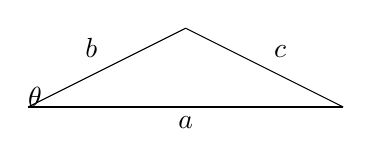
\begin{tikzpicture}
            \coordinate (C) at (0, 0);
            \coordinate (B) at (4, 0);
            \coordinate (A) at (2, 1);

            \draw (C) -- (B) node [midway,anchor=north] {$a$};
            \draw (B) -- (A) node [midway,anchor=south west] {$c$};
            \draw (A) -- (C) node [midway,anchor=south east] {$b$};

            \tkzMarkAngle[size=0.3cm,mark=|](C,A,B)
            \tkzLabelAngle[pos=0.6](C,A,B) {$\theta$}
        \end{tikzpicture}
    \caption{Law of Cosines}
    \label{fig:law-of-cosines}
    \end{figure}

    We can use this to extend our notion of angle beyond $\R^2$. Let $a = \norm{x - y}$, $b = \norm{x}$, and $c = \norm{y}$ as in Figure \ref{fig:vector-law-of-cosines}. Then $\norm{x - y}^2 = \langle x-y, x-y \rangle = \langle x, x\rangle - 2\langle x, y\rangle + \langle y, y \rangle = \norm{x}^2 - 2\langle x, y \rangle + \norm{y}^2$. Applying the Law of Cosines, we obtain
    \[\cos(\theta) = \frac{\langle x, y \rangle}{\norm{x}\norm{y}}.\]

    \begin{figure}[ht!]
        \centering
        \begin{tikzpicture}
            \coordinate (C) at (0, 0);
            \coordinate (B) at (4, 0);
            \coordinate (A) at (2, 1);

            \begin{scope}[decoration={
                markings,
                mark=at position 0.5 with {\arrow{>}}}
                ]
                \draw[postaction={decorate}] (A)--(B) node [midway,anchor=south west] {$y$};
                \draw[postaction={decorate}] (A)--(C) node [midway,anchor=south east] {$x$};
                \draw[postaction={decorate}] (B)--(C) node [midway,anchor=north] {$x-y$};
            \end{scope}
        \end{tikzpicture}
    \caption{Vector triangle}
    \label{fig:vector-law-of-cosines}
    \end{figure}
\end{rmk}

\begin{defn}
    Let $(V, \langle,\rangle)$ be an inner product space over $F$, and let $x, y \in V$ be non-zero vectors. We define the \emph{angle} between $x$ and $y$ as
    \[\theta = \arccos\left(\frac{\langle x, y \rangle}{\norm{x}\norm{y}}\right).\]
\end{defn}

\begin{defn}
    Let $(V, \langle,\rangle)$ be an inner product space over $F$. A subset $S \subseteq V$ is
    \begin{itemize}
        \item \emph{orthogonal} if $x$ and $y$ are orthogonal for every $x, y \in S$ where $x \neq y$,
        \item \emph{normal} if $\norm{x} = 1$ for all $x \in S$,
        \item \emph{orthonormal} if $S$ is both orthogonal and normal.
    \end{itemize}
\end{defn}

\begin{rmk}
    If $x \in V$ is non-zero, then $\frac{x}{\norm{x}}$ is a unit vector since
    \[\norm{\frac{x}{\norm{x}}} = \frac{1}{\norm{x}}\norm{x} = 1.\]
\end{rmk}

\begin{prop}
    Let $(V, \langle,\rangle)$ be an inner product space over $F$, and let $S \subseteq V$ be orthogonal. If all $x \in S$ are non-zero then $S$ is linearly independent.
\end{prop}

\begin{proof}
    Suppose that $a_1v_1 + \cdots + a_kv_k = \vec{0}$ for some distinct $v_1, \ldots, v_k \in S$ and non-zero $a_1, \ldots, a_k \in F$. Fix $j \in \{1, \ldots, k\}$. Then
    \begin{align*}
        0 &= \langle \vec{0}, v_j \rangle = \langle a_1v_1 + \cdots + a_kv_k, v_j \rangle \\
        &= a_1\langle v_1, v_j \rangle + \cdots + a_k\langle v_k, v_j \rangle.
    \end{align*}
    Since $S$ is orthogonal, all $\langle v_i, v_j \rangle$ must be zero except for $i = j$. Therefore, $0 = a_j\langle v_j, v_j \rangle$. Since $v_j \neq \vec{0}$, $\langle v_j, v_j \rangle \neq 0$ and therefore $a_j = 0$. It follows that all $a_1, \ldots, a_k = 0$ and so $S$ is linearly independent.
\end{proof}

\begin{exmp}
    \[S = \left\{(1, 1, 0), (1, -1, 1), (-1, 1, 2)\right\}\]
    $S$ can easily to verified to be orthogonal, and so it must be linearly independent and therefore forms a basis for $\R^3$. Furthermore, it follows that
    \[B = \left\langle \frac{1}{\sqrt{2}}(1, 1, 0), \frac{1}{\sqrt{3}}(1, -1, 1), \frac{1}{\sqrt{6}}(-1, 1, 2)\right\rangle\]
    is an orthonormal basis for $\R^3$.
\end{exmp}

\begin{thm}\label{orthogonal-decomposition}
    Let $(V, \langle,\rangle)$ be an inner product space over $F$, and let $S = \{v_1, \ldots, v_k\}$ be an orthogonal set of non-zero vectors. Given any $y \in \spanset{S}$, then $y$ is the sum of the orthogonal components of $y$ along each $v_i$:
    \[y = \sum_{i=1}^{k}\frac{\langle y, v_i\rangle}{\norm{v_i}^2}v_i.\]
\end{thm}

\begin{proof}
    Since $y \in \spanset{S}$, we know that $y = \sum_{i=1}^{k}a_iv_i$ for some $a_i \in F$. Fix $j \in \{1, \ldots, k\}$. Then
    \[\langle y, v_j \rangle = \left\langle \sum_{i=1}^{k}a_iv_i, v_j \right\rangle = a_j\langle v_j, v_j \rangle, \textrm{ and so } a_j = \frac{\langle y, v_j \rangle}{\langle v_j, v_j \rangle} = \frac{\langle y, v_j\rangle}{\norm{v_j}^2}.\]
\end{proof}

\begin{cor}\label{orthonormal-decomposition}
    If $S$ is orthonormal, then $y = \sum_{i=1}^{k}\langle y, v_i\rangle v_i$.
\end{cor}

\begin{thm}{Gram-Schmidt Process}\label{gram-schmidt-process}\proofbreak
    Let $(V, \langle,\rangle)$ be an inner product space over $F$, and let $S =\{w_1, \ldots, w_n\}$ be a linearly independent set. Define $S' = \{v_1, \ldots, v_n\}$ by $v_1 = w_1$, and for $k > 1$ by
    \[v_k = w_k - \sum_{i=1}^{k-1}\frac{\langle w_k, v_i\rangle}{\norm{v_i}^2}v_i.\]
    Then $S'$ is an orthogonal set of non-zero vectors, and has the same span as $S$.
\end{thm}

\begin{proof}
    Let $S_k = \{w_1, \ldots, w_k\}$ and $S_{k}' = \{v_1, \ldots, v_k\}$. We will show by induction on $k$ that $S_{k}'$ is an orthogonal set of non-zero vectors such that $\spanset{S_k} = \spanset{S_{k}'}$.

    When $k = 1$, $S_k = \{w_1\} = \{v_1\} = S_{k}'$ and so $S_{k}'$ is vacuously orthogonal, and $v_1 \neq \vec{0}$. Assume that the statement holds for some $k-1 \geq 1$. Then
    \begin{align*}
        v_k = w_k - \sum_{i=1}^{k-1}\frac{\langle w_k, v_i\rangle}{\norm{v_i}^2}v_i.
    \end{align*}
    Suppose that $v_k = \vec{0}$, then
    \[w_k = \sum_{i=1}^{k-1}\frac{\langle w_k, v_i\rangle}{\norm{v_i}^2}v_i,\]
    and so $w_k \in \spanset{S_{k-1}'} = \spanset{S_{k-1}}$. However, this violates the assumption that $S_{k-1}$ is linearly independent. Therefore, $v_k \neq \vec{0}$. For $j \in \{1, \ldots, k-1\}$,
    \begin{align*}
        \langle v_k, v_j \rangle = \langle w_k, v_j \rangle - \sum_{i=1}^{k-1}\frac{\langle w_k, v_i}{\norm{v_i}^2}\langle v_i, v_j \rangle = \langle w_k, v_j \rangle - \frac{\langle w_k, v_j}{\norm{v_j}^2}\langle v_j, v_j \rangle = 0,
    \end{align*}
    and so $S_{k}'$ must be orthogonal.

    By construction, $v_k \in \spanset{S_k}$, and so $\spanset{S_{k}'}$ is a subspace of $\spanset{S_{k}}$. Since $S_{k}$ and $S_{k}'$ are linearly independent and each have $k$ vectors, they must have the same dimension. Then by Theorem \ref{subspace-is-finite}, it follows that $\spanset{S_{k}'} = \spanset{S_k}$.
\end{proof}

\begin{cor}
    Let $(V, \langle,\rangle)$ be a finite dimensional inner product space over $F$. Then $V$ has an orthonormal basis.
\end{cor}

\begin{proof}
    Let $B$ be any basis for $V$. Apply the Gram-Schmidt process to obtain an orthogonal basis $B'$, and finally normalize each vector in $B'$ to obtain an orthonormal basis for $V$.
\end{proof}

\begin{exmp}
    Consider $\R^4$ with the standard dot product, and let
    \[S = \{(1, 0, 1, 0), (1, 1, 1, 1), (0, 1, 2, 1)\}.\]
    We start with $v_1 = w_1 = (1, 0, 1, 0)$, and then
    \[v_2 = w_2 - \frac{\langle w_2, v_1\rangle}{\norm{v_1}^2}v_1 = (1, 1, 1, 1) - \frac{2}{2}(1, 0, 1, 0) = (0, 1, 0, 1),\]
    \[v_3 = w_3 - \frac{\langle w_3, v_1 \rangle}{\norm{v_1}^2}v_1 - \frac{\langle w_3, v_2 \rangle}{\norm{v_2}^2}v_2 = (0, 1, 2, 1) - \frac{2}{2}(1, 0, 1, 0) - \frac{2}{2}(0, 1, 0, 1) = (-1, 0, 1, 0).\]
    Therefore, $\{(1, 0, 1, 0), (0, 1, 0, 1), (-1, 0, 1, 0)\}$ is an orthogonal set, and
    \[\left\{\frac{1}{\sqrt{2}}(1, 0, 1, 0), \frac{1}{\sqrt{2}}(0, 1, 0, 1), \frac{1}{\sqrt{2}}(-1, 0, 1, 0)\right\}\]
    is an orthonormal set.
\end{exmp}

\begin{defn}
    Let $(V, \langle,\rangle)$ be an inner product space over $F$, and $S \subseteq V$ an arbitrary non-empty set. The \emph{orthogonal complement} of $S$ is the set
    \[S^{\perp} = \left\{x \in V \compbar \langle x, y \rangle = 0 \,\forall y \in S \right\}.\]
\end{defn}

\begin{lemma}\label{orthogonal-complement-is-subspace}
    Let $(V, \langle,\rangle)$ be an inner product space over $F$, and $S \subseteq V$ an arbitrary non-empty set. Then $S^{\perp}$ is a vector subspace of $V$.
\end{lemma}

\begin{proof}
    Since $\langle \vec{0}, y \rangle = 0$ for all $y \in S$, we know that $\vec{0} \in S^{\perp}$. For any $x, z \in S^{\perp}$ and $r \in F$, and for all $y \in S$
    \[\langle x + rz, y \rangle = \langle x, y \rangle + r\langle z, y \rangle = 0 + r(0) = 0,\]
    so $x + rz \in S^{\perp}$. Therefore, $S^{\perp}$ by a subspace of $V$ by Proposition \ref{subspace-proof}.
\end{proof}

\begin{exmp}
    Let $V$ be a vector space with an arbitrary inner product. Then $\{\vec{0}\}^{\perp} = V$ and $V^{\perp} = \{\vec{0}\}$.
\end{exmp}

\begin{exmp}
    In $\R^3$ with the standard dot product, $\{e_3\}^{\perp} = \spanset{\{e_1, e_2\}}$.
\end{exmp}

\begin{lemma}\label{orthogonal-complement-of-orthogonal-complement}
    Let $(V, \langle,\rangle)$ be an inner product space over $F$, and $S \subseteq V$ an arbitrary non-empty set. Then $S \subseteq \left(S^{\perp}\right)^{\perp}$.
\end{lemma}

\begin{proof}
    Fix some $x \in S$. For any $y \in S^{\perp}$, we know that $\langle x, y \rangle = 0$ by definition. But $\langle y, x \rangle = \overline{\langle x, y \rangle} = \overline{0} = 0$, and so $x \in \left(S^{\perp}\right)^{\perp}$.
\end{proof}

\begin{thm}
    Let $(V, \langle,\rangle)$ be a finite dimensional inner product space over $F$ and $W \subseteq V$ a subspace.
    \begin{enumerate}
        \item $W \intersection W^{\perp} = \{\vec{0}\}$.
        \item Any $x \in V$ can be uniquely expressed as $x = w + u$ where $w \in W$ and $u \in W^{\perp}$.
        \item The dimension of $V$ is the sum of the dimensions of $W$ and $W^{\perp}$.
        \item $W = \left(W^{\perp}\right)^{\perp}$.
    \end{enumerate}
\end{thm}

\begin{proof}\proofbreak
    (1) Let $x \in W \intersection W^{\perp}$. By definition, $\langle x, x \rangle = 0$, so $x = \vec{0}$.

    Use the Gram-Schmidt process to construct an orthonormal basis $\{v_1, \ldots, v_n\}$ for $V$ such that $\{v_1, \ldots, v_k\}$ forms an orthonormal basis for $W$. We will show that $\{v_{k+1}, \ldots, v_n\}$ forms an orthonormal basis for $W^{\perp}$. First note that $\{v_{k+1}, \ldots, v_n\}$ is linearly independent by construction. Let $x \in V$, then by Corollary \ref{orthonormal-decomposition}
    \[x = \sum_{i=1}^{n}\langle x, v_i\rangle v_i.\] In the case that $x \in W^{\perp}$, by definition $\langle x, v_i\rangle = 0$ and so $x \in \spanset{\{v_{k+1}, v_n\}}$, and so $W^{\perp} \subseteq \spanset{\{v_{k+1}, \ldots, v_n\}}$. Furthermore, for $y \in \spanset{\{v_{k+1}, \ldots, v_n\}}$ we know that \[y = \sum_{i={k+1}}^{n}\langle x, v_i\rangle v_i = \sum_{i=1}^{n}\langle x, v_i\rangle v_i.\] Since $\{v_1, \ldots, v_k\}$ is linearly independent, it follows that $\langle y, v_i \rangle = 0$ and so $\langle y, w \rangle = 0$ for all $w \in \spanset{\{v_1, \ldots, v_k\}} = W$. Therefore, $y \in W^{\perp}$ and so $\spanset{\{v_{k+1}, \ldots, v_n\}} \subseteq W^{\perp}$, implying that $\spanset{\{v_{k+1}, \ldots, v_n\}} = W^{\perp}$. It follows that $\{v_{k+1}, v_n\}$ is a basis for $W^{\perp}$ by definition.

    (2) Let $x \in V$, then \[x = \sum_{i=1}^{n}\langle x, v_i \rangle v_i = \sum_{i=1}^{k}\langle x, v_i \rangle v_i = \sum_{i={k+1}}^{n}\langle x, v_i \rangle v_i = w + u,\] where $w \in W$ and $u \in W^{\perp}$. Therefore, there is at least one way to express $x \in V$ as $x = w + u$ where $w \in W$ and $u \in W^{\perp}$. To show uniqueness, assume that $x = w + u = w' + u'$ where $w, w' \in W$ and $u + u' \in W^{\perp}$. Then $w + u = w' + u'$, and so $w - w' = u - u' \in W \intersection W^{\perp} = \{\vec{0}\}$ by (1), and so $w = w'$ and $u = u'$.

    (3) Since $\{v_1, \ldots, v_k\}$ is a basis for $W$ and $\{v_{k+1}, \ldots, v_n\}$ is a basis for $W^{\perp}$, it necessarily follows that the dimension of $V$ is the sum of the dimensions of $W$ and $W^{\perp}$.

    (4) By (3), we know that $\dim V = \dim W + \dim W^{\perp}$ and also that $\dim V = \dim W^{\perp} + \dim\left(W^{\perp}\right)^{\perp}$, so $\dim W = \dim \left(W^{\perp}\right)^{\perp}$. Since $W$ and $\left(W^{\perp}\right)$ are both subspaces of $V$ by Lemma \ref{orthogonal-complement-is-subspace} and $W \subseteq \left(W^{\perp}\right)^{\perp}$ by Lemma \ref{orthogonal-complement-of-orthogonal-complement}, we know that $\dim W = \dim \left(W^{\perp}\right)^{\perp}$ implies that $W = \left(W^{\perp}\right)^{\perp}$ by Proposition \ref{subspace-is-finite}.
\end{proof}

\begin{defn}
    Let $V$ be a vector space over $F$, and $W$ and $U$ subspaces of $V$. If $W \intersection U = \{\vec{0}\}$, and every $x \in V$ can be uniquely expressed as $x = w + u$ with $w \in W$ and $u \in U$, we say that $V$ is the \emph{direct sum} of $W$ and $U$, denoted as $V = W \directsum U$.
\end{defn}

\begin{exmp}
    Let $(V, \langle,\rangle)$ be a finite dimensional inner product space over $F$ and $W \subseteq V$ a subspace. Then $V = W \directsum W^{\perp}$.
\end{exmp}

\begin{exmp}
    $\R^3 = \spanset{\{e_1, e_2\}} \directsum \spanset{\{e_3\}}$.
\end{exmp}

\begin{defn}
    Let $(V, \langle,\rangle)$ be a finite dimensional inner product space over $F$ and $W \subseteq V$ a subspace. For $x = w + u \in V$ where $w \in W$ and $u \in W^{\perp}$, we say that $w$ is the \emph{orthogonal projection} of $x$ onto $W$.
\end{defn}

\begin{rmk}
    If $\{v_1, \ldots, v_k\}$ is an orthonormal basis for $W$ and $x \in V$, then the orthogonal projection $w$ of $x$ on $W$ is
    \[w = \sum_{i=1}^{k}\langle x, v_i \rangle v_i, \;\textrm{and}\, u = x - w.\]
\end{rmk}

\begin{prop}\label{ortho-proj-closest}
    Let $(V, \langle,\rangle)$ be a finite dimensional inner product space over $F$ and $W \subseteq V$ a subspace. The orthogonal projection $w$ of $x$ is the unique vector in $W$ that is closest to $x$ --- that is, $\norm{x - w} \leq \norm{x - y}$ for all $y \in W$, with equality if and only if $y = w$.
\end{prop}

\begin{proof}
    Let $w$ be the orthogonal projection of $x$ on $W$, and $u = x - w \in W^{\perp}$. Since $w, y \in W$ we have $w - y \in W$, and so $w - y$ is orthogonal to $u$. Then $\norm{x-y}^2 = \norm{w + u - y}^2$ and by the Pythagorean Theorem \ref{pythagorean-thm} we have $\norm{w + u - y}^2 = \norm{w - y}^2 + \norm{u^2}$. It follows that
    \[\norm{x-y}^2 = \norm{w - y}^2 + \norm{u^2} \geq \norm{u^2} = \norm{x - w}^2.\]
\end{proof}

\section{Norms}

\begin{defn}
    Let $V$ be a vector space over $\R$ or $\C$. A \emph{norm} on $V$ is a function $\norm{\cdot}: V \to \R$ satisfying, for all $x, y \in V$ and scalar $s$:
    \begin{itemize}
        \item absolute homogeneity: $\norm{sx} = \abs{s}\norm{x}$,
        \item positive definiteness: $\norm{x} = 0$ if and only if $x = \vec{0}$,
        \item sub-additivity (triangle inequality): $\norm{x + y} \leq \norm{x} + \norm{y}$.
    \end{itemize}
\end{defn}

\begin{defn}
    We define the $\ell_p$ norm, for real $p \geq 1$ and $x = (x_1, x_2, \ldots, x_n)$, by
    \begin{align*}
        \norm{x}_p = \left[\sum_{i=1}^{n}\abs{x_i}^p\right]^{1/p}.
    \end{align*}    
\end{defn}

\begin{exmp}
    The $\ell_1$ is the taxi-cab norm, while $\ell_2$ is the Euclidean norm. We can also show that
    \begin{align*}
        \norm{x}_{\infty} = \lim_{p\to\infty}\norm{x}_p
    \end{align*}
    defines a norm, called the infinity norm.
\end{exmp}

\begin{prop}{Reverse triangle inequality}\label{reverse-triangle-inequality}\proofbreak
    Let $\norm{\cdot}$ be a norm on a vector space $V$. Then for all $x, y \in V$,
    \begin{align*}
        \abs{\norm{x} - \norm{y}} \leq \norm{x - y}.
    \end{align*}
\end{prop}

\begin{proof}
    Consider applying the triangle inequality to $x - y$ and $y$. We have
    \begin{align*}
        \norm{x - y + y} \leq \norm{x - y} + \norm{y},
    \end{align*}
    so $\norm{x} - \norm{y} \leq \norm{x - y}$. By interchanging the roles of $x$ and $y$ we also have $\norm{y} - \norm{x} \leq \norm{y - x}$. Since
    \begin{align*}
        \norm{y - x} = \norm{(-1)(x-y)} = \abs{-1}\norm{x - y} = \norm{x - y},
    \end{align*}
    we have
    \begin{align*}
        \abs{\norm{x} - \norm{y}} \leq \norm{x - y}.
    \end{align*}
\end{proof}

\begin{defn}
    The \emph{spectral radius} of an $n \times n$ matrix $A$ is the magnitude of the largest eigenvalue of $A$.
\end{defn}

\begin{prop}
    Let $A \in M_{n \times n}(\R)$. Then for any consistent matrix norm, $\rho(A) \leq \norm{A}$.
\end{prop}

\begin{proof}
    Let $v$ be an eigenvector of $A$ with associated eigenvalue $\lambda$. Since $\norm{\cdot}$ is consistent with some vector norm $\norm{\cdot}$, we know that
    \begin{align*}
        \norm{Av} \leq \norm{A}\norm{v}.
    \end{align*}
    Therefore,
    \begin{align*}
        \frac{\norm{Av}}{\norm{v}} \leq \norm{A},
    \end{align*}
    and since
    \begin{align*}
        \frac{\norm{Av}}{\norm{v}} = \frac{\abs{\lambda}\norm{v}}{\norm{v}} = \abs{\lambda},
    \end{align*}
    it follows that $\abs{\lambda} \leq \norm{A}$ for all eigenvalues $\lambda$ of $A$ and so $\rho(A) \leq \norm{A}$.
\end{proof}

\begin{thm}
    Let $A \in M_{n \times n}(\R)$, and consider any $\varepsilon > 0$. There exists a natural matrix norm (which may differ depending on $A$), denoted by $\norm{\cdot}_{\varepsilon, A}$, such that
    \begin{align*}
        \norm{A} \leq \rho(A) + \varepsilon.
    \end{align*}
\end{thm}

\section{Adjoints}

\begin{defn}
    Let $(V, \langle, \rangle_V)$ and $(W, \langle, \rangle_W)$ be inner product spaces over $F$. Given a linear transformation $T: V \to W$, the \emph{adjoint} of $T$ is the linear transformation $T^{*}: W \to V$ satisfying \[\langle T(V), W\rangle_W = \langle V, T^{*}(W)\rangle_V.\]
\end{defn}

\begin{lemma}Representation Theorem\label{adjoint-representation-theorem}\proofbreak
    Let $(V, \langle,\rangle)$ be a finite dimensional inner product space over $F$, and let $\ell: V \to F$ be a linear function. There exists unique $w \in V$ such that $\ell(v) = \langle v, w \rangle$ for all $v \in V$.
\end{lemma}

\begin{proof}
    Let $\{v_1, \ldots, v_n\}$ be an orthonormal basis for $V$. For any $v \in V$, we know that
    \[v = \sum_{i=1}^{n}\langle v, v_i \rangle v_i,\]
    and so it follows that
    \[\ell(v) = \ell\left(\sum_{i=1}^{n}\langle v, v_i \rangle v_i\right) = \sum_{i=1}^{n}\langle v, v_i \rangle \ell(v_i) = \left\langle v, \sum_{i=1}^{n}\overline{\ell(v_i)v_i} \right\rangle.\]
    Therefore, $w = \sum_{i=1}^{n}\overline{\ell(v_i)v_i}$. Uniqueness follows from Theorem \ref{inner-product-properties} (5).
\end{proof}

\begin{thm}\label{adjoint-existence-uniqueness}
    Let $(V, \langle, \rangle)$ and $(W, \langle, \rangle)$ be inner product spaces over $F$, and $T: V \to W$ be a linear transformation. The adjoint $T^*$ of $T$ exists and is unique.
\end{thm}

\begin{proof}
    For given $w \in W$, consider $\ell: V \to F$ defined by $v \mapsto \langle T(v), w \rangle$. Since $T$ is linear in $v$ and $\langle,\rangle$ is linear in the first argument, $\ell$ is linear in $v$. By Lemma \ref{adjoint-representation-theorem}, there exists unique $y \in V$ such that $\langle T(v), w \rangle = \ell(v) = \langle v, y \rangle$. Define $T^*(w) = y$ to obtain a function $T^*: W \to V$.

    All that remains is for us to show that $T^*$ is indeed a linear function. Note that
    \begin{align*}
        \langle v, T^*(w_1 + rw_2) \rangle &= \langle T(v), w_1 + rw_2 \rangle = \langle T(v), w_1 \rangle + \overline{r}\langle T(v), w_2 \rangle \\
        &= \langle v, T^*(w_1) \rangle + \overline{r}\langle v, T^*(w_2) \rangle = \langle v, T^*(w_1) + rT^*(w_2) \rangle.
    \end{align*}
    It follows that $T^*(w_1 + rw_2) = T^*(w_1) + rT^*(w_2)$ by Theorem \ref{inner-product-properties} (5). Therefore, $T^*$ is linear and is the unique function satisfying $\langle T(v), w \rangle = \langle v, T^*(w) \rangle$.
\end{proof}

\begin{prop}
    Let $(V, \langle, \rangle)$ and $(W, \langle, \rangle)$ be inner product spaces over $F$, and $T: V \to W$ be a linear transformation. Then
    \[(T^*)^* = T.\]
\end{prop}

\begin{proof}
    \[\langle T(v), w \rangle = \langle v, T^*(w) \rangle = \langle v, T^*(w) \rangle = \overline{\langle T^*(w), v \rangle} = \overline{\langle w, (T^*)^*(v) \rangle} = \langle (T^*)^*(v), w \rangle\]
\end{proof}

\begin{lemma}
    Let $A \in M_{m \times n}(F)$, $x \in F^n$, and $y \in F^m$. Then $\langle Ax, y \rangle_m = \langle x, A^{*}y \rangle_n$, where $\langle,\rangle_k$ denotes the standard dot product with in $F^k$.
\end{lemma}

\begin{proof}
    \[\langle x, A^{*}y\rangle_n = (A^{*}y)^{*}x = y^{*}(A^*)^{*}x = y^*Ax = \langle Ax, y \rangle_m\]
\end{proof}

\begin{rmk}
    Let $A$ be a matrix and $L_A$ the corresponding linear transformation. This lemma states that the linear transformation corresponding to the conjugate transpose of $A^{*}$ satisfies the adjoint property for the standard dot product, and so by Theorem \ref{adjoint-existence-uniqueness} is the unique adjoint. This is,
    \[\left(L_A\right)^{*} = L_{A^{*}}.\]
\end{rmk}

\begin{lemma}
    Let $A \in M_{m \times n}(F)$. Then the ranks of $A$ and $A^{*}A$ are equal.
\end{lemma}

\begin{proof}
    Note that $A$ is $m \times n$, so $A^*A$ is an $n \times n$ square matrix. If we can show that the nullity of $L_A$ is equal to the nullity $L_{A^*A}$, then by the Rank-nullity Theorem \ref{rank-nullity} $A$ and $A^*A$ must have the same rank.

    For any $x$ in the kernel (null-space) of $L_A$, we have $Ax = \vec{0}$, and so $A^*Ax = A^*\vec{0} = \vec{0}$, and so the kernel of $L_A$ is a subset of the kernel of $L_{A^*A}$. Now consider $x$ in the kernel of $L_{A^*A}$. We know that
    \begin{align*}
        \langle Ax, Ax \rangle = \langle x, A^*Ax \rangle = \langle x, \vec{0} \rangle = 0,
    \end{align*}
    and so $Ax = \vec{0}$ by Theorem \ref{inner-product-properties} (4). Therefore, the kernel of $L_{A^*A}$ is also a subset of the kernel of $L_A$, and so the kernels (and therefore the nullities) of $L_A$ and $L_{A^*A}$ are equal.
\end{proof}

\begin{rmk}
    Note that since $A^*A$ is an $n \times n$ matrix, it is invertible precisely when the rank of $A$ is $n$.
\end{rmk}

\begin{thm}
    Let $A \in M_{m \times n}(F)$ and $y \in F^n$. Then there exists $x_0 \in F^n$ such that
    \[\norm{y - Ax_0} \leq \norm{y - Ax}.\]
    Furthermore, if $A$ has rank $n$, then $x_0$ is unique and is given by $x_0 = (A^*A)^{-1}A^*y$.
\end{thm}

\begin{proof}
    Let $W$ be the column space of $A$, and let $w_0$ be the orthogonal projection of $y$ onto $W$. We know that $w_0$ is the unique vector in the column space of $A$ that satisfies $\norm{y - w_0} \leq \norm{y - w}$ for all $w$ in the column space of by Proposition \ref{ortho-proj-closest}. Since $w_0$ is the in column space of $A$, we are guaranteed the existence (although not the uniqueness) of $x_0$, which is simply the coordinates of $w_0$ in terms of the columns of $A$. If $A$ has rank $n$ then the columns of $A$ form a basis for the column space and so $x_0$ must be unique.

    When $A$ has rank $n$, then $x_0$ satisfies $y = Ax_0 + u$ where $u \in W^{\perp}$ and $Ax \in W$. Therefore, $y - Ax_0 = u \in W^{\perp}$, so for all $x \in F^n$ we have
    \[\langle Ax, y - Ax_0 \rangle = 0,\]
    and so $\langle x, A^*y - A^*Ax_0 \rangle = 0$. Then since this equation is true for all $x \in F^n$ we must have $A^*y - A^*Ax_0 = \vec{0}$, and so $A^*Ax_0 = A^*y$. Since $A^*A$ is invertible when $A$ has rank $n$, we finally have
    \[x_0 = \left(A^*A\right)^{-1}A^*y.\]
\end{proof}

\begin{defn}
    A matrix $P \in M_{n \times n}(\C)$ is said to be \emph{orthogonal} when the columns of $P$ form an orthogonal basis for $\C^n$.
\end{defn}

\begin{lemma}
    A matrix $P \in M_{n \times n}(\C)$ is orthogonal if and only if $P$ is invertible and $P^{-1} = \transposeof{P}$.
\end{lemma}

\begin{proof}
    Let $v_i$ denote the $i$th column of $P$ (and therefore the $i$th column of $\transposeof{P}$). Note that $P$ is orthogonal is equivalent to saying that $v_i \cdot v_j = 1$ precisely when $i = j$ and $v_i \cdot v_j = 0$ otherwise. Therefore, $P$ is orthogonal is equivalent to $\transposeof{P}P = I_n$ and since $\transposeof{P}$ is also orthogonal, $P\transposeof{P} = I_n$. It follows that $P$ is orthogonal is precisely equivalent to $P$ is invertible and $P^{-1} = \transposeof{P}$.
\end{proof}

\begin{rmk}
    If $P$ is orthogonal, then so is $\transposeof{P}$. If $S$ and $R$ are orthogonal, then $SR$ is orthogonal since $(SR)\transposeof{(SR)} = S(R\transposeof{R})\transposeof{S} = S\transposeof{S} = I$.
\end{rmk}

\begin{thm}Spectral Theorem\label{spectral-theorem}\proofbreak
    Let $A \in M_{n \times n}(\R)$. If $A$ is symmetric ($A = \transposeof{A}$), then $A$ is diagonalizable and there exists an orthogonal basis for $\R^n$ composed of eigenvectors of $A$.
\end{thm}

\begin{proof}
    Consider $A \in M_{n \times n}(\C)$. We know that $A$ must have at least one eigenvalue $\lambda \in \C$ by the Fundamental theorem of algebra \ref{algebra-fundamental-theorem}.
    \begin{align*}
        \lambda\langle x, x\rangle = \langle Ax, x \rangle = \langle x, A^*x\rangle
    \end{align*}
    Since $A \in M_{n \times n}(\R)$, $A^* = \transposeof{A}$. Then $A = \transposeof{A}$ implies that $A^* = A$, so $\langle x, A^*x \rangle = \langle x, Ax \rangle$. We then have
    \begin{align*}
        \lambda\langle x, x\rangle = \langle x, \lambda x\rangle = \overline{\lambda}\langle x, x \rangle.
    \end{align*}
    Since $x \neq 0$, it follows that $\lambda = \overline{\lambda}$ and so $\lambda \in \R$. Therefore, all eigenvalues of $A$ are real and so $A$ has at least one real eigenvalue.

    We will proceed by induction on $n$. First, a $1 \times 1$ matrix $A = (a)$ is trivially both symmetric and diagonalizable, and $\{(1)\}$ is a basis for $\R^1$ that is vacuously orthogonal and composed of eigenvectors of $A$. Now assume that for $m \leq n-1$, any $m \times m$ real symmetric matrix is diagonalizable, and there exists an orthogonal basis for $\R^m$ composed of its eigenvectors.
    
    Let $\lambda_1$ be a real eigenvalue and $v_1$ be the corresponding eigenvector. Complete to an ordered orthogonal basis $B = \langle v_1, \ldots, v_n \rangle$ for $\R^n$. Let $Q$ be a matrix whose $i$th column is $v_i$, and let
    $\tilde{A} = [L_A]_{B}^{B}$. Then $\tilde{A} = Q^{-1}AQ = \transposeof{Q}AQ$. Note that $\tilde{A}$ is symmetric: $\transposeof{\left(\transposeof{Q}AQ\right)} = \transposeof{Q}\transposeof{A}\transposeof{\left(\transposeof{Q}\right)} = \transposeof{Q}AQ = \tilde{A}$.

    Since $Av_1 = \lambda_1v_1$, we know that
    \[\tilde{A} = \left(\begin{array}{c|ccc}
        \lambda_1 & 0 & \cdots & 0 \\
        \hline
        0 & & & \\
        \vdots & & & \\
        0 & \largeblock{3}{2.2}{$B$}
    \end{array}\right),\]
    where $B$ is an $(n-1)\times(n-1)$ real symmetric matrix. By assumption, there exists an $(n-1)\times(n-1)$ diagonal matrix $E$ and $T$ an $(n-1)\times(n-1)$ orthogonal matrix such that $B = TET^{-1} = TE\transposeof{T}$. Then
    \[\tilde{A} = \left(\begin{array}{c|ccc}
        1 & 0 & \cdots & 0 \\
        \hline
        0 & & & \\
        \vdots & & & \\
        0 & \largeblock{3}{2.0}{$T$}
    \end{array}\right)
    \left(\begin{array}{c|ccc}
        \lambda_1 & 0 & \cdots & 0 \\
        \hline
        0 & & & \\
        \vdots & & & \\
        0 & \largeblock{3}{2.0}{$E$}
    \end{array}\right)
    \left(\begin{array}{c|ccc}
        1 & 0 & \cdots & 0 \\
        \hline
        0 & & & \\
        \vdots & & & \\
        0 & \largeblock{3}{2.7}{$\transposeof{T}$}
    \end{array}\right) = SD\transposeof{S},\]
    where $S$, $D$, and $\transposeof{S}$ are simply the three matrices in the product. Then,
    \[A = Q\tilde{A}\transposeof{Q} = QSD\transposeof{S}\transposeof{Q} = (QS)D\transposeof{(QS)} = (QS)D(QS)^{-1}.\]
    Note that $D$ is diagonal since $E$ is, and $S$ (and $\transposeof{S}$) are orthogonal since $T$ (and $\transposeof{T}$) is. Since $Q$ and $S$ are orthogonal, so is their product $QS$. Since $D$ is a diagonal matrix of eigenvalues, the columns of $QS$ are necessarily eigenvectors of $A$, and so the columns of $QS$ form an orthogonal basis of eigenvectors.
\end{proof}

\begin{defn}
    A symmetric matrix $A \in M_{n\times n}(\R)$ is \emph{positive definite} if $\transposeof{z}Mz$ is strictly positive for \emph{every} non-zero real $z \in \R^n$, and \emph{positive semidefinite} if $\transposeof{z}Mz$ is positive or zero for every non-zero real $z \in \R^n$. Negative definite and negative semidefinite are defined similarly.
    
    For Hermitian matrices $H \in M_{n\times n}(\C)$, these are defined similarly using $z^{*}Hz$.

    A matrix that is neither positive nor negative (semi)definite is said to be \emph{indefinite}.
\end{defn}

\begin{thm}\label{positive-semidefinite-criteria}
    Let $A \in M_{n \times n}(\R)$ be a symmetric matrix. Then $A$ is positive definite, positive semidefinite, negative definite, or negative semidefinite if and only if the eigenvalues of $A$ are real and strictly positive, non-negative, strictly negative, or non-positive respectively.
\end{thm}

\begin{proof}
    By the Spectral Theorem \ref{spectral-theorem}, we know that there is an orthogonal basis $B = \langle v_1, \ldots, v_n\rangle$ for $\R^n$ composed of eigenvectors of $A$, where $\lambda_1, \ldots, \lambda_n$ are the associated real eigenvalues. For any non-zero $z \in \R^n$, consider
    \begin{align*}
        z &= a_1v_1 + \cdots + a_nv_n.
    \end{align*}
    Therefore,
    \begin{align*}
        \transposeof{z}Az &= \transposeof{z}A\left(a_1v_1 + \cdots + a_nv_n\right) \\
        &= \transposeof{z}\left(a_1\lambda_1v_1 + \cdots + a_n\lambda_{n}v_n\right).
    \end{align*}
    Since $B$ is orthogonal, $\transposeof{v_i}v_j = 0$ whenever $i \neq j$, and so
    \begin{align*}
        \transposeof{z}Az &= a_1^2\lambda_1\transposeof{v_1}v_1 + \cdots + a_n^2\lambda_{n}\transposeof{v_n}v_n.
    \end{align*}
    Since $z \in \R^n$ we have $a_i \in \R$, and so $a_i^2 \geq 0$ and of course $v_i \in \R^n$ and so $v_i^2 > 0$. Therefore, the sign of $\transposeof{z}Az$ depends only on the signs of $\lambda_i$.
\end{proof}

\begin{cor}
    If a matrix is positive semidefinite and invertible (so no eigenvalues can't be zero) then it must be positive definite.
\end{cor}

\setchaptergraphic{}

\chapter{Numerical Analysis}
\label{ch:numerical}

\section{Floating Point Approximations}

Given $x \in \R$, and a floating point representation $\hat{x}$, we define the relative error to be $r = \frac{\abs{\hat{x}-x}}{x}$. We then define the \emph{significant figures} of $\hat{x}$ to be maximum $m \in \N$ such that $10^{m}r \leq 5$.

Consider a method to calculate from value. Let
\begin{itemize}
    \item $x$ be the input,
    \item $\hat{x}$ be the approximated input,
    \item $f(x)$ be the correct value of the output,
    \item $\hat{f}$ approximate of $f$.
\end{itemize}
Then the total error is
\begin{align*}
    \hat{f}\left(\hat{x}\right) - f(x) = \underbrace{\hat{f}\left(\hat{x}\right) - f(\hat{x})}_{\textrm{Computational error}} + \overbrace{f\left(\hat{x}\right) - f(x)}^{\textrm{Propagated error}}.
\end{align*}

\begin{exmp}
    Consider a $\mathbb{C}^2$ function $f: \R \to \R$. Using a small value for $h$, we can approximate the derivative of $f$ as
    \begin{align*}
        D_{h}f(x) = \frac{f(x + h) - f(x)}{h}.
    \end{align*}

    The computational error in this approximation is
    \begin{align*}
        D_{h}f(x) - f'(x).
    \end{align*}
\end{exmp}

\begin{exmp}
    Consider a function $f: \R \times \R \to \R$ given by $f(x, y) = xy$. If the approximation error for $x$ and $y$ is $\delta_x$ and $\delta_y$ respectively, then
    \begin{align*}
        \hat{x} &= x + \delta_x, \\
        \hat{y} &= y + \delta_y.
    \end{align*}

    Therefore, the propagated error is simply
    \begin{align*}
        f\left(\hat{x}, \hat{y}\right) - f(x, y) &= x\delta_y + y\delta_x + \delta_x\delta_y,
    \end{align*}
    and so the relative propagated error is
    \begin{align*}
        \frac{f\left(\hat{x}, \hat{y}\right) - f(x, y)}{f(x, y)} = \frac{x\delta_y + y\delta_x + \delta_x\delta_y}{xy} = \frac{\delta_x}{x} + \frac{\delta_y}{y} + \frac{\delta_x\delta_y}{xy}.
    \end{align*}
    Under the reasonable assumption that $\delta_x \ll x$ and $\delta_y \ll y$, the term $\frac{\delta_x\delta_y}{xy}$ is negligible, and so the relative error of $xy$ is roughly $R(x) + R(y)$.
\end{exmp}

\section{Algorithms and Convergence}

\begin{defn}
    A mathematical problem is \emph{well-posed} or \emph{stable} when a solution \emph{exists}, is \emph{unique}, and is \emph{continuous} with respect to the input.
\end{defn}

\begin{defn}
    Given a function $f$, the \emph{condition number}, or \emph{conditioning number}, is the supremum of ratio of the relative change in output to the relative change in input.
\end{defn}

\begin{exmp}
    Let $f: \R \to \R$ be a continuous function. Then the condition number, denoted by $K_f(x)$, is
    \begin{align*}
        K_f(x) = \lim_{x' \to x}\abs{\frac{\left[f(x') - f(x)\right]/f(x)}{\left(x'-x\right)/x}} = \abs{\frac{x}{f(x)}f'(x)}.
    \end{align*}
\end{exmp}

\begin{defn}
    Now consider $f: \R^d \to R$ where $f$ is $C^2$. The absolute change in the output can be approximated at the first order as
    \begin{align*}
        \delta_{y} \approx \sum_{i=1}^{d}\frac{\partial f}{\partial x_i}(x)\delta_{x_i} = \left\langle \nabla f(x), \delta_{x} \right\rangle.
    \end{align*}
    The relative change is then
    \begin{align*}
        \varepsilon_{y} \approx \sum_{i=1}^{d}\frac{\partial f}{\partial x_i}(x)\frac{\delta_{x_i}}{f(x)}.
    \end{align*}
    Let $\varepsilon_{x_i} = \frac{x_i'-x_i}{x_i}$, then $\delta_{x_i} = \varepsilon_{x_i}x_i$, so
    \begin{align*}
        \varepsilon_{y} \approx \sum_{i=1}^{d}\frac{\partial f}{\partial x_i}(x)\frac{x_i}{f(x)}\varepsilon_{x_i}.
    \end{align*}
\end{defn}

\begin{thm}\label{matrix-condition-number}
    Let $A$ be a non-singular matrix, and $\norm{\cdot}$ be an induced norm. Then
    \begin{align*}
        \kappa(A) = \norm{A}\norm{A^{-1}}.
    \end{align*}
\end{thm}

\begin{proof}
    By definition, the conditioning number at $b$ is
    \begin{align*}
        \sup_{\delta b \neq 0}\frac{\norm{A^{-1}(b + \delta b) - A^{-1}b}}{\norm{A^{-1}b}}\frac{\norm{b}}{\norm{\delta b}}.
    \end{align*}
    Notice that
    \begin{align*}
        \frac{\norm{A^{-1}(b + \delta b) - A^{-1}b}}{\norm{A^{-1}b}} = \frac{\norm{A^{-1}\delta b}}{\norm{A^{-1}b}}.
    \end{align*}
    Therefore, the supremum of this across all $b$ is
    \begin{align*}
        \kappa(A) = \sup_{b \neq 0,\delta b \neq 0}\frac{\norm{A^{-1}\delta b}}{\norm{A^{-1}b}}\frac{\norm{b}}{\norm{\delta b}}.
    \end{align*}
    Let $c = A^{-1}b$, then we can separate the supremums over $c$ and $\delta b$ to obtain
    \begin{align*}
        \kappa(A) = \sup_{c \neq 0,\delta b \neq 0}\frac{\norm{A^{-1}\delta b}}{\norm{c}}\frac{\norm{Ac}}{\norm{\delta b}} = \left[\sup_{c \neq 0}\frac{\norm{Ac}}{\norm{c}}\right]\left[\sup_{\delta b \neq 0}\frac{\norm{A^{-1}\delta b}}{\norm{\delta b}}\right].
    \end{align*}
    Then by Theorem \ref{induced-norm} we have
    \begin{align*}
        \kappa(A) = \norm{A}\norm{A^{-1}}.
    \end{align*}
\end{proof}

\begin{exmp}
    Consider $f(x_1, x_2) = x_1 - x_2$. Then
    \begin{align*}
        K_f(x_1, x_2) = \abs{\frac{x_1}{x_1 - x_2}} + \abs{\frac{x_2}{x_1 - x_2}}.
    \end{align*}
\end{exmp}

\begin{defn}
    Let $f(x)$ be a function with condition number $K_f$, and let $x_y = g(x_n)$ be an iterative algorithm, where $K_n(y_n)$ is the condition number of $g(x_n)$. Then we define
    \begin{align*}
        \hat{K}(y) = \sup_{n \leq N}K_n(y_n),
    \end{align*}
    and say that an algorithm is \emph{numerically stable} when
    \begin{align*}
        \hat{K}(y) \lesssim 2K_f.
    \end{align*}
\end{defn}

\begin{defn}
    The transformation of an ill-posed problem into a well-posed one is \emph{regularization}.
\end{defn}

\begin{exmp}
    Consider a linear system $Ax = b$, where $\det A = 0$. If $b$ is in the null space of $A$, then there are infinite solutions, and otherwise there are no solutions. Therefore it is not a well-posed problem. However, if we consider
    \begin{align*}
        \min_{x}\norm{Ax - b},
    \end{align*}
    this clearly always has a solution. Furthermore, when a solution exists to $Ax - b$ it will coincide.
\end{exmp}

\begin{defn}
    Consider functions $f(h)$ and $g(h)$ such that $g(h)$ goes to zero as $h$ does. We use Landau big-$O$ notation and say that
    \begin{align*}
        f(h) = L + O(g(h))
    \end{align*}
    if there exists $h_0$ and $C$ such that $\abs{f(h) - L} < Cg(h)$ for all $\abs{h} < h_0$.
\end{defn}

\begin{defn}
    Consider an iterative algorithm $f_n(x_n)$ to compute a function $f(x)$. We say that it is a \emph{$p$th order approximation} when
    \begin{align*}
        \abs{f_n(x_n) - f(x)} = O\left(\frac{1}{n^p}\right).
    \end{align*}
\end{defn}

\begin{rmk}
    When we increase $n$ (the number of iterations used) by a factor of ten, a $p$th order approximation will gain $p$ significant figures.
\end{rmk}

\begin{defn}
    Consider an iterative algorithm $f_n(x_n)$ to compute a function $f(x)$. If
    \begin{align*}
        \lim_{n\to\infty}\frac{\abs{f_{n+1}(x_{n+1}) - f(x)}}{\abs{f_{n}(x_{n}) - f(x)}^{p}} = \mu
    \end{align*}
    for some $\mu > 0$, we say that $f_n$ converges with rate of order $p$.
\end{defn}

\begin{rmk}
    When an algorithm converges with a rate of order $p$, we say that we have
    \begin{itemize}
        \item \emph{linear convergence} if $p = 1$ and $\mu < 1$,
        \item \emph{quadratic convergence} if $p = 2$,
        \item \emph{cubic convergence} if $p = 3$.
    \end{itemize}
\end{rmk}

\section{Matrix Factorization}

\begin{defn}
    LU composition
\end{defn}

\begin{defn}
    An $n \times n$ matrix $A$ is said to be \emph{diagonally dominant} if, for all $1 \leq i \leq n$,
    \begin{align*}
        \abs{A_{ii}} \geq \sum_{j\neq i}\abs{A_{ij}}.
    \end{align*}
    $A$ is furthermore \emph{strictly} diagonally dominant if, for all $1 \leq i \leq n$,
    \begin{align*}
        \abs{A_{ii}} > \sum_{j\neq i}\abs{A_{ij}}.
    \end{align*}
\end{defn}

\begin{thm}
    Positive definite $\iff$ $\forall k A_k$ is positive definite.
    Positive definite $\iff$ $\forall k \det A_k > 0$ \emph{and} $A$ is Hermitian.
    Positive definite $\iff$ $A$ is Hermitian and Gaussian elimination can be performed without permutations.
\end{thm}

\begin{thm}{Cholesky Factorization}\label{cholesky-factorization}\proofbreak
    Let $A \in M_{n \times n}(\C)$ be a positive definite matrix. There exists a unique lower triangular matrix $L \in M_{n \times n}(\C)$ such that $L_{ii} > 0$ such that $A = LL^{*}$. 
\end{thm}

\begin{proof}
    We will proceed by induction on $n$. In the base case $n=1$, we simply have $A = [a]$, and so for $L = [l]$, $LL^{*} = l\overline{l}$, and since $l_{ii}$ must be real we have $l = \sqrt{a}$. Since $A$ is positive definite, by \ref{positive-semidefinite-criteria} it follows that $a > 0$ and so $\sqrt{a} \in \R$.

    Assume that a unique decomposition exists for all $0 \leq n < k$ for some $k$. Consider any positive definite matrix $A \in M_{k \times k}(\C)$. We can write
    \[
        A = \begin{pmatrix}
            A_{k-1} & b \\
            \overline{b} & a_{kk}
        \end{pmatrix}
    \]
\end{proof}

\begin{defn}
    A \emph{band matrix} is a particular type of sparse matrix in which the non-zero entries occur only within $p$ diagonals above the major diagonal, and $q$ diagonals above. Formally, $A \in M_{n \times n}$ is a \emph{band matrix} if there exists \emph{unique} $p, q \in \{1, \ldots, n\}$ such that $A_{ij}$ is zero whenever $j - i \geq p$ or $i - j \geq q$.
\end{defn}

\begin{rmk}
    Gaussian elimination is always successful as long as a pivot can be found.
\end{rmk}

\begin{defn}
    In \emph{partial pivoting}, at step $k$ of Gaussian elimination, we choose
    \begin{align*}
        i_{k} = \argmax_{k\leq i\leq n}\abs{a_{ik}^{(k)}}
    \end{align*}
    as the pivot. If $i_k > k$, we swap rows $k$ and $i_k$, and then proceed as normal. We can construct a permutation matrix $P$ such that $PA = LU$.
\end{defn}

\begin{defn}
    In \emph{complete pivoting}, at step $k$ of Gaussian elimination, we choose
    \begin{align*}
        (i_{k}, j_{k}) = \argmax_{k\leq i, j\leq n}\abs{a_{ik}^{(k)}}
    \end{align*}
    as the pivot. If $i_k > k$, we swap rows $k$ and $i_k$, if $j_k > k$, we swap columns $k$ and $j_k$, and then proceed as normal. We can construct permutation matrices $P$ and $Q$ such that $PAQ = LU$.
\end{defn}

\begin{rmk}
    While complete pivoting may be theoretically superior, partial pivoting yields similar results and so is preferred in practice.
\end{rmk}

\begin{thm}
    Let $A \in M_{n \times n}(\C)$ be Hermitian. There exists a unitary matrix $U$ such that $A = UDU^{*}$, where
    \begin{align*}
        D = \begin{pmatrix}
            \lambda_1 & 0 & \cdots & 0 \\
            0 & \lambda_2 & \cdots & 0 \\
            \vdots & \vdots & \ddots & \vdots \\
            0 & 0 & \cdots & \lambda_n \\
        \end{pmatrix}
    \end{align*}
    and $\lambda_1, \ldots, \lambda_n$ are the eigenvalues (with multiplicity) of $A$.
\end{thm}

\begin{lemma}\label{singular-non-difference-inequality}
    Consider any singular matrix $B$, and a proper (and therefore induced) norm $\norm{\cdot}$, then
    \begin{align*}
        \norm{A^{-1}}\norm{A - B} \geq 1.
    \end{align*}
\end{lemma}

\begin{proof}
    Since $\norm{\cdot}$ is proper by assumption,
    \begin{align*}
        \norm{A^{-1}B - I_n} = \norm{A^{-1}(A-B)} \leq \norm{A^{-1}}\norm{A-B}.
    \end{align*}
    For convenience, let $C = A^{-1}B - I_n$. If we can show $\norm{C} \geq 1$ we are done. For any $x \in F^n$, note that since $C$ is induced we have
    \begin{align*}
        \norm{C} \geq \frac{\norm{Cx}}{\norm{x}} = \frac{\norm{A^{-1}Bx - x}}{\norm{x}} \geq \abs{\frac{\norm{A^{-1}Bx}}{\norm{x}} - \frac{\norm{x}}{\norm{x}}}.
    \end{align*}
    Since $B$ is singular, there exists $x$ such that $Bx = 0$ and $x \neq 0$ so $\norm{x} \neq 0$. Then for $x \in \mathcal{N}(B)$
    \begin{align*}
        \norm{C} \geq \abs{\frac{0}{\norm{x}} - \frac{\norm{x}}{\norm{x}}} = 1.
    \end{align*}
\end{proof}

\begin{thm}
    The condition number of a matrix $A$ can be characterized by
    \begin{align*}
        \frac{1}{\kappa(A)} = \min\left\{\frac{\norm{A - B}}{\norm{A}}: \det(B) = 0\right\}.
    \end{align*}
\end{thm}

\begin{proof}
    Let $A$ be a non-singular matrix, and $B$ be any singular matrix, and $\norm{\cdot}$ an induced norm. Then by Lemma \ref{singular-non-difference-inequality}
    \begin{align*}
        \frac{\norm{A - B}}{\norm{A}} \geq \frac{1}{\norm{A}\norm{A^{-1}}}.
    \end{align*}
    and since $\norm{A}\norm{A^{-1}} = \kappa(A)$ by Theorem \ref{matrix-condition-number} we find that $1/\kappa(A)$ is at most the infimum of the set.

    Proving that this minimum is actually attained requires further tools from functional analysis, see ``Numerical Linear Algebra'' by W. Kahan for the proof.
\end{proof}

\begin{defn}
    Given a linear system $Ax = b$ with solution $x_0$ and an approximate solution $\tilde{x}$, let the \emph{residual} of $\tilde{x}$ be $r = A\tilde{x} - Ax_0 = A\tilde{x} - b$ and let $e = \tilde{x} - x_0 = A^{-1}r$.
\end{defn}

\begin{prop}
    Let $Ax = b$ be a linear system with solution $x$, and let $r$ be the residual of some approximate solution. Then by consistency of the norm, we obtain
    \begin{itemize}
        \item $\norm{r} \leq \norm{A}\norm{e}$,
        \item $\norm{e} \leq \norm{A^{-1}}\norm{r}$,
        \item $\norm{b} \leq \norm{A}\norm{x}$,
        \item $\norm{x} \leq \norm{A^{-1}}\norm{b}$.
    \end{itemize}
\end{prop}

\begin{prop}
    The relative error in an approximate solution $\tilde{x}$ can be founded by
    \begin{align*}
        \frac{\norm{e}}{\norm{x_0}} \leq \kappa(A)\frac{\norm{r}}{\norm{b}}.
    \end{align*}
\end{prop}

\begin{proof}
    Note that $\norm{e} \leq \norm{A^{-1}}\norm{r}$ and $\norm{b} \leq \norm{A}\norm{x_0}$ so $\norm{x_0} \geq \norm{b}/\norm{A}$. Therefore,
    \begin{align*}
        \frac{\norm{e}}{\norm{x_0}} \leq \norm{A}\norm{A^{-1}}\frac{\norm{r}}{\norm{b}} = \kappa(A)\frac{\norm{r}}{\norm{b}}.
    \end{align*}
\end{proof}

\begin{defn}
    Consider a matrix $A$. The \emph{singular values} of $A$, denoted by $\sigma(A)$, are the eigenvalues of $A^{*}A$.
\end{defn}

\begin{rmk}
    We know that $\norm{A}_2 = \sqrt{\rho(A^{*}A)}$, in which case $\kappa(A)$ is
    \begin{align*}
        \frac{\max_{\lambda \in \sigma(A)}\abs{\lambda}}{\min_{\lambda \in \sigma(A)}\abs{\lambda}}.
    \end{align*}
\end{rmk}

\begin{thm}
    Consider a linear system $Ax = b$ with a induced matrix norm and $A$ non-singular. For perturbations $\delta A$ and $\delta b$ such that
    \begin{align*}
        \norm{\delta A} < \frac{1}{\norm{A^{-1}}},
    \end{align*}
    the following hold:
    \begin{itemize}
        \item $A + \delta A$ is non-singular,
        \item $(A + \delta A)(x + \delta x) = (b + \delta b)$,
    \end{itemize}
    and
    \begin{align*}
        \frac{\norm{\delta x}}{\norm{x}} \leq \frac{\kappa(A)}{1 - \kappa(A)\frac{\norm{\delta A}}{\norm{A}}}\left(\frac{\norm{\delta A}}{\norm{A}} + \frac{\norm{\delta b}}{\norm{b}}\right).
    \end{align*}
\end{thm}

\begin{proof}
    Notice that
    \begin{align*}
        \norm{\delta A} \leq \frac{1}{\norm{A^{-1}}} \implies \norm{A^{-1}\delta A} \leq \norm{A^{-1}}\norm{\delta A} < 1,
    \end{align*}
    and
    \begin{align*}
        A + \delta A = A\left(I_n + A^{-1}\delta A\right)
    \end{align*}
    Let $M = -A^{-2}\delta A$, so $\norm{A} < 1$, and then
    \begin{align*}
        I_n + A^{-1}\delta A)
    \end{align*}

    {\large\color{red}Finish proof}
\end{proof}

\begin{defn}
    Consider an $n \times n$ invertible matrix $A$, then the \emph{growth factor} of $A$ is
    \begin{align*}
        \rho = \frac{1}{\norm{A}_{\infty}}\max_{1 \leq i,j,k \leq n} \abs{A_{ij}^{(k)}},
    \end{align*}
    where $A^{(k)}$ is the $k$th iterate obtained via Gaussian elimination.
\end{defn}

\begin{thm}
    Consider the linear system $Ax = b$, where $A$ is an $n \times n$ invertible matrix, and its $LU$ decomposition obtained via Gaussian elimination. Assume presence of numerical error, so
    \begin{align*}
        LU = A + E
    \end{align*}
    for some $n \times n$ matrix $E$. Then
    \begin{align*}
        \frac{\norm{E}_{\infty}}{\norm{A}_{\infty}} \leq n^2\rho\delta,
    \end{align*}
    where $\rho$ is the growth factor of $A$ and $\delta$ is the machine epsilon.
\end{thm}

\begin{rmk}
    Using different pivoting strategies, the growth factor $\rho$ may be controlled to an extent. Using \emph{complete pivoting}, we can bound it as
    \begin{align*}
        \rho \leq (1.8)n^{\ln(n)/4}.
    \end{align*}
\end{rmk}

\section{Fixed-Point Methods}

We will attempt to transform the linear system $Ax = b$ into the form $x = Tx + c$, the so-called ``fixed-point'' form of $x$, since the solutions are the fixed-points of the affine transformation.

Note that for all invertible $n \times n$ matrices $B$, where we have $Ax = b$ for some vector $b$, we can write $Ax = b$ as $Bx + (A - B)x = b$, which in turn may be rewritten as $x = B^{-1}(B-A)x + B^{-1}b = (I_n - B^{-1}A)x + B^{-1}b$.

\begin{defn}
    Select (arbitrary) point $x^{(0)} \in \R^{d}$ and recursively define
    \begin{align*}
        x^{(k+1)} &= Tx^{(k)} + c = \left(I_n - B^{-1}A\right)x^{(k)} + B^{-1}b
    \end{align*}
    which is equivalent to
    \begin{align*}
        B\left(x^{(k+1)} - x^{(k)}\right) = b - Ax^{(k)}.
    \end{align*}
    We call the expression on the right hand side the \emph{residual}. Various \emph{stoppping criterion} for termination of this algorithm are possible, such as when the relative (or absolute) residual falls beneath a chosen threshold.
\end{defn}

\begin{defn}{Jacobi method}\proofbreak
    Consider the decomposition
    \begin{align*}
        A = -L + D - U,
    \end{align*}
    where $-L$, $D$, $-U$ are lower triangular, diagonal, and upper triangular matrices respectively. In the \emph{Jacobi method}, we choose $B = D$, and so
    \begin{align*}
        T_{J} = I - B^{-1}A = I - D^{-1}A = I-D^{-1}(D - L - U) = D^{-1}(L + U).
    \end{align*}
    Notice that we then have
    \begin{align*}
        x^{(k + 1)}_{i} = \frac{-\sum_{j\neq i}A_{ij}x^{(k_j)} + b_i}{A_{ii}}.
    \end{align*}
\end{defn}

\begin{defn}{Gauss-Seidel method}\proofbreak
    Consider the decomposition
    \begin{align*}
        A = -L + D - U,
    \end{align*}
    where $-L$, $D$, $-U$ are lower triangular, diagonal, and upper triangular matrices respectively. In the \emph{Gauss-Seidel method}, we choose $B = D - L$, and so
    \begin{align*}
        T_{G} = I - \left(D - L\right)^{-1}\left(D - L - U\right) = I - I - \left(D - L\right)^{1}\left(-U\right) = \left(D-L\right)^{-1}U.
    \end{align*}
    Notice that we then have
    \begin{align*}
        x^{(k + 1)}_{i} = \frac{-\sum_{j=1}^{i-1}A_{ij}x^{(k_j+1)} - \sum_{j= i+1}^{n}A_{ij}x^{(k_j)} + b_i}{A_{ii}}.
    \end{align*}
\end{defn}

\begin{rmk}
    In general, the Gauss-Seidel method tends to perform better than the Jacobi method.
\end{rmk}

\begin{thm}\label{fixed-point-convergence}
    Let $T \in M_{n \times n}(\R)$ be invertible, and let $x_0 \in \R^n$. The sequence $x^{(k+1)} = Tx^{(k)} + c$ will converge to a solution for \emph{any} choice of $x_0$ if and only if $\rho(T) < 1$. This solution is unique and does not depend on choice of initial $x^{(0)}$.
\end{thm}

\begin{proof}
    Let $\norm{\cdot}$ be a proper norm. First, we will see that a unique fixed-point always exists and is unique. Since $\rho(T) < 1$, then $I - T$ is invertible and so $(I - T)x = c$ has a unique solution. Now let us turn to convergence.

    ($\implies$) Let $x$ be a solution, and consider the largest eigenvalue in absolute value $\rho(A)$ with associated eigenvector $u$. Then let $x_0 = x - u$, and so $x - x^{(k)} = \rho(A)^{(k)}u$, so $x{(k)}$ converges only if $\rho(A) < 1$.

    ($\impliedby$) First, we will prove that $x - x^{(k)} = T^{k}(x - x_0)$ by induction. In the base case, this is trivially true since $T^0 = I$. Then, assuming $x - x^{(k)} = T^{k}(x - x_0)$, we then have
    \[T\left[x - x^{(k)}\right] = T\left[T^{k}(x - x_0)\right],\]
    and so
    \[Tx + c - Tx^{(k)} - c = T^{k+1}(x - x_0).\]
    Since $x$ is by construction a fixed point of $f(v) = Tv + c$, it follows that $Tx + c = x$, and by definition $Tx^{(k)} + c = x^{(k+1)}$, so we have
    \begin{align*}
        x - x^{(k+1)} = T^{k+1}(x - x_0).
    \end{align*}
    Now that we have shown that $x - x^{(k)} = T^{k}(x - x_0)$ for $k \geq 0$, it follows since the norm is proper that $\norm{T^{k}(x - x_0)} \leq \norm{T^k}\norm{x-x_0}$. We know this converges to zero as $k$ goes to infinity since $\rho(T) < 1$, and so $x^{(k)}$ converges to $x$.
\end{proof}

\begin{prop}
    Let $\norm{\cdot}$ be a induced norm such that $\norm{T} < 1$ then $x^{(k)}$ converges and $\norm{x - x^{k}} \leq \norm{T}^{k}\norm{x - x_0}$ and $\norm{x - x^{k}} \leq \frac{\norm{T}^{k}}{1 - \norm{T}}\norm{x^{(1)} - x^{0}}$.
\end{prop}

\begin{thm}
    Let $A$ be an $n \times n$ matrix. If $A$ is strictly diagonally dominant, then the Jacobi and Gauss-Seidel methods converges for all $x^{(0)} \in \R^n$, and furthermore
    \begin{align*}
        \norm{T_{G}}_{\infty} \leq \norm{T_{J}}_{\infty} < 1.
    \end{align*}
\end{thm}

\begin{proof}
    Recall $T_{J}$ is defined to be $D^{-1}(L + U)$, so
    \begin{align*}
        \norm{T_{J}}_{\infty} = \max_{1\leq i \leq n}\frac{1}{D_{ii}}\sum_{j=1}^{n}(L + U)_{ji} = \max_{1\leq i \leq n}\frac{1}{A_{ii}}\sum_{j \neq i}A_{ji}.
    \end{align*}
    Since $A$ is strictly diagonally dominant, $A_{ii}$ is strictly greater than the sum for all $i$, and so
    \begin{align*}
        \norm{T_{J}}_{\infty} < 1.
    \end{align*}
\end{proof}

\begin{defn}
    Let $A$ be an $n \times n$ matrix. We say that $A$ is \emph{irreducible} when there \emph{does not} exist a permutation matrix $P$ such that $\transposeof{P}AP$ is a block upper triangular matrix
    \begin{align*}
        \left[\begin{array}{c|c}
            \tilde{A}_{11} & \tilde{A}_{12} \\
            \hline
            \raisebox{0pt}[12pt][0pt]{\scalebox{1.5}{$0$}} & \tilde{A}_{22}
        \end{array}\right]
    \end{align*}
    such that $\tilde{A}_{11} \in M_{p\times p}$ and $\tilde{A}_{22} \in M_{q \times q}$ where $p + q = n$, and $n > p, q \geq 1$. Note that $\tilde{A}_{ij}$ may be anything -- in particular they may contain zero entries.
\end{defn}

\begin{prop}
    An $n \times n$ matrix $A$ is irreducible if and only if the directed graph $G(A)$, of which $A$ is the adjacency matrix, is strongly connected.
\end{prop}

\begin{proof}
    First, note that $G(\transposeof{P}AP)$ is isomorphic to $G(A)$ --- that is, the two matrices are the adjacency matrices of the same graphs, up to order of vertices. To see this, let $\sigma$ be the permutation induced by $P$ --- that is, $P_{ij} = \delta_{i\sigma(j)}$. Then
    \begin{align*}
        AP_{\sigma_{i}j} &= \sum_{k=1}^{n}A_{\sigma(i)k}P(kj) = A_{\sigma(i)\sigma(j)}, \\
        \transposeof{P}AP_{ij} &= \sum_{k=1}^{n}\transposeof{P}_{ik}AP_{kj} = AP_{\sigma(i)j}.
    \end{align*}
    Therefore, $\transposeof{P}AP_{ij} = A_{\sigma(i)\sigma(j)}$, so $G(A)$ and $G(\transposeof{P}AP)$ are isomorphic since permutations are bijections. We know that if $A$ is isomorphic to $B$, then $A$ is strongly connected if and only if $B$ is strongly connected.

    To construct the adjacency matrix, we must have an index on the vertices $V_i$. Then we may consider a path from $V_i$ to $V_j$. Such a path must correspond to a sequence $a_1, a_2, \ldots, a_k$ such that $a_1 = n$, $a_k = 1$, and $\transposeof{P}AP_{a_{\ell}a_{\ell+1}} = 1$ for all $\ell \in \{1, \ldots, k-1\}$. Since $\transposeof{P}AP_{a_{\ell}a_{\ell+1}} = 0$ if $a_{\ell} > p$ and $a_{\ell+1} \leq n-q = p$, it follows that $a_{\ell+1} > p$ whenever $a_{\ell} > p$. Since $a_1 = n > p$ it would then follow that $a_k > p$. Therefore, no such path may exist if $\transposeof{P}AP$ is block upper triangular, and so if \emph{any} permutation matrix $P$ makes $\transposeof{P}AP$ block upper triangular then $G(A)$ cannot be strongly connected.

    Assume that $G(A)$ is not strongly connected, so there exists vertices $\alpha$ and $\beta$ such that there is no path from $\alpha$ to $\beta$. Let $V_{\alpha}$ be the set of all vertices $v$ such that there is a path from $\alpha$ to $v$, and let $V_{\beta}$ be the set of all vertices $v$ such that there is a path from $v$ to $\beta$. Note that $V_{\alpha}$ and $V_{\beta}$ must be disjoint by assumption. Let $p = \abs{V_{\beta}}$, and consider a permutation $\sigma$ which sends $V_{\beta}$ to $\{1, \ldots, p\}$ and $V_{\alpha}$ to $\{p+1, \ldots, n\}$. Notice that ${\transposeof{P_{\sigma}}AP_{\sigma}}_{ij} = 0$ whenever $p+1 \leq i \leq n$ and $1 \leq j \leq p$. Therefore, there exists $\sigma$ such that $\transposeof{P_{\sigma}}AP_{\sigma}$ is block upper triangular whenever $G(A)$ is not strongly connected.
\end{proof}

\begin{defn}
    An $n \times n$ matrix is \emph{irreducibly diagonally dominant} when it is irreducible, (weakly) diagonally dominant, and additionally there exists $i$ such that
    \begin{align*}
        \abs{A_{ii}} > \sum_{j\neq i}\abs{A_{ij}}.
    \end{align*}
\end{defn}

\begin{prop}
    Let $A$ be an $n \times n$ matrix. If $A$ is irreducibly diagonally dominant, then the Jacobi method converges for all $x^{(0)} \in \R^n$.
\end{prop}

\begin{defn}{SOR method}\proofbreak
    Consider the decomposition
    \begin{align*}
        A = -L + D - U,
    \end{align*}
    where $-L$, $D$, $-U$ are lower triangular, diagonal, and upper triangular matrices respectively. In the \emph{SOR method} (successive over-relaxtion), we choose
    \begin{align*}
        B(\omega) = \frac{1}{\omega}\left(D - \omega L\right).
    \end{align*}
    \begin{align*}
        T(\omega) = I - \left(\frac{1}{\omega}\left(D - \omega L\right)\right)^{-1}\left(D - L - U\right) = \left(D - \omega L\right)^{-1}\left[(1-\omega)D + \omega U\right].
    \end{align*}
\end{defn}

\begin{thm}{Kahan's Theorem}\label{kahans-theorem}\proofbreak
    If $\det D \neq 0$, then
    \begin{align*}
        \rho\left(T(\omega)\right) \geq \abs{\omega - 1}.
    \end{align*}
\end{thm}

\begin{proof}
    \begin{align*}
        \det\left(T(\omega)\right) = \frac{\det\left((1-\omega)D + \omega U\right)}{\det\left(D - \omega L\right)} = \frac{\left(1-\omega\right)^{n}\det\left(D\right)}{\det\left(D\right)} = \left(1 - \omega\right)^{n}.
    \end{align*}
\end{proof}

\begin{thm}
    If $A$ is positive definite and $0 < \omega < 2$, then $p(T(\omega)) < 1$.
\end{thm}

\setchaptergraphic{
    \begin{tikzpicture}[
        shorten >=1pt,>={Stealth[round]},
        node distance=2.5 cm,
        every state/.style={draw=blue!50,very thick,fill=blue!20}
    ]
        \node[initial, state]   (A)                    {$q_0$};
        \node[state, accepting] (B) [right of=A]       {$q_1$};
        \node[state, accepting] (C) [above right of=B] {$q_2$};
        \node[state]            (R) [below right of=B] {$q_3$};

        \path[->] (A) edge [above]                  node [align=center] {0,1} (B)
                  (B) edge [above left, bend left]  node [align=center] {1} (C)
                      edge [below left]             node [align=center] {0} (R)
                  (C) edge [below right, bend left] node [align=center] {0,1} (B)
                  (R) edge [loop right]             node [align=center] {0,1} ();
    \end{tikzpicture}
}

\chapter{Computation Theory}
\label{ch:computation}

\section{Finite Automata}

\begin{defn}
    An \emph{alphabet} is a non-empty set whose elements are referred to as \emph{symbols}. \emph{Strings} (or \emph{words}) over a given alphabet are finite sequences of symbols from the alphabet. A \emph{language} is a set of strings over an alphabet.
\end{defn}

\begin{rmk}
    Alphabets and languages may be non-finite, but strings are generally considered to only include finite sequences. The empty string will be denoted by $\emptystring$.
\end{rmk}

\begin{defn}
    Let $\Sigma$ be an alphabet. Then the language consisting of all strings over $\Sigma$ of length $n$ is denoted by $\Sigma^{n}$. The \emph{Kleene closure} of $\Sigma$ is
    \begin{align*}
        \Sigma^{*} = \bigunion_{i\in\N}\Sigma^{i}.
    \end{align*}
\end{defn}

\begin{defn}
    Given languages $A$ and $B$, the \emph{concatenation} of $A$ and $B$, denoted by $A \concat B$, is
    \begin{align*}
        A \concat B = \left\{\alpha\beta : \alpha \in A, \beta \in B \right\},
    \end{align*}
    where $\alpha\beta$ is the string formed by concatenating $\alpha$ and $\beta$.
\end{defn}

\begin{defn}
    Let $L$ be a language. We can also apply the Kleene star operator to this language, creating its Kleene closure $L^*$ by defining
    \begin{align*}
        L^0 &= \{\emptystring\}, \\
        L^{i+1} &= L^{i} \concat L, \\
        L^{*} &= \bigunion_{i \geq 0}L^{i}.
    \end{align*}
\end{defn}

\begin{defn}
    A (deterministic) \emph{finite automaton} is a $5$-tuple $(Q, \Sigma, \delta, q_0, F)$, where
    \begin{itemize}
        \item $Q$ is a finite set of \emph{states},
        \item $\Sigma$ is an alphabet,
        \item $\delta: Q \times \Sigma \to Q$ is the \emph{transition function},
        \item $q_0 \in Q$ is the \emph{start state},
        \item $F \subseteq Q$ are the \emph{accept states}.
    \end{itemize}
    An automaton starts in state $q_0$, and is given an input consisting over a string over $\Sigma$. For each symbol $s$ in the input, the automaton moves from state $q$ to state $\delta(q, s)$. Once the end of the input is reached, if the state $q$ of the automaton is an accept state --- that is, $q \in F$, then the automaton is said to have \emph{accepted} the input.
\end{defn}

\begin{defn}
    The \emph{language accepted by} a finite automaton $M$ is a language $A$ consisting of all strings over $\Sigma$ that are accepted by the finite automaton. We denote this by $L(M) = A$. A \emph{regular language} is any language accepted by some finite automaton.
\end{defn}

\begin{rmk}
    Finite automata can be represented as a graph, where states are represented as nodes, and transitions are edges between states, labelled by the symbol that triggers the transition. When graphically representing a finite automaton as a graph, accept states may be represented as double-circled nodes.
\end{rmk}

\begin{exmp}
    \begin{figure}[ht!]
        \centering
        \begin{tikzpicture}[
            shorten >=1pt,>={Stealth[round]},
            node distance=2 cm,
            every state/.style={draw=blue!50,very thick,fill=blue!20}
        ]
            \node[initial, state]   (S) {$q_0$};
            \node[state]            (0) [right of=S] {$q_1$};
            \node[state]            (00) [right of=0] {$q_2$};
            \node[state, accepting] (001) [right of=00] {$q_3$};
    
            \path[->] (S)   edge [above, bend left]     node [align=center] {0} (0)
                      (S)   edge [loop below]           node [align=center] {1} ()
                      (0)   edge [above, bend left]     node [align=center] {0} (00)
                            edge [above, bend left]     node [align=center] {1} (S)
                      (00)  edge [loop above]           node [align=center] {0} ()
                            edge [above, bend left]     node [align=center] {1} (001)
                      (001) edge [below, bend left]     node [align=center] {0} (0)
                            edge [above, bend right=60] node [align=center] {1} (S);
        \end{tikzpicture}
        \caption{Example finite automaton}
        \label{fig:example-finite-automaton}
    \end{figure}

    In the finite automaton shown in Figure \ref{fig:example-finite-automaton}, $Q = \left\{q_0, q_1, q_2, q_3\right\}$, $\Sigma = \left\{0, 1\right\}$, $F = \{q_3\}$, and $\delta$ is
    \begin{center}
        \begin{tabular}{|c||c|c|}
            \hline
            \thead{$\delta$} & \thead{$0$}    & \thead{$1$} \\
            \hline\hline
            \textsc{$q_0$}   & \textsc{$q_1$} & \textsc{$q_0$} \\
            \hline
            \textsc{$q_1$}   & \textsc{$q_2$} & \textsc{$q_0$} \\
            \hline
            \textsc{$q_2$}   & \textsc{$q_2$} & \textsc{$q_3$} \\
            \hline
            \textsc{$q_3$}   & \textsc{$q_1$} & \textsc{$q_0$} \\
            \hline
        \end{tabular}.
    \end{center}

    This language accepted by this finite automaton is the set of all binary strings which end with \texttt{001}. We can use an inductive proof on the length of the longest input to prove this.
\end{exmp}

\begin{prop}\label{regular-language-complement}
    Let $A$ be a regular language, then $\complementof{A}$ is also a regular lanaguage.
\end{prop}

\begin{proof}
    Let $M = (Q, \Sigma, \delta, s_0, F)$ be a finite automaton that recognizes $A$, and define
    \begin{align*}
        M' = (Q, \Sigma, \delta, s_0, Q \setminus F).
    \end{align*}
    For any $w \in \Sigma^{*}$, we can see that $M$ and $M'$ reach the same final state, let this be $s_f$. Since $s_f \in F$ if and only if $s_f \in Q \setminus F$, it follows that $M'$ accepts $w$ if and only if $M$ \emph{does not}, therefore the regular language that $M'$ recognizes is precisely $\complementof{A}$.
\end{proof}

\begin{thm}\label{regular-language-union-intersection}
    Let $A$ and $B$ be regular languages, then $A \union B$ and $A \intersection B$ are also regular languages.
\end{thm}

\begin{proof}
    Let $\Sigma$ be the union of the alphabets of $A$ and $B$. Since $A$ and $B$ are regular, we know that there exists finite automata $M_A = \left(Q_1, \Sigma, \delta_1, s_1, F_1\right)$ and $M_B = \left(Q_2, \Sigma, \delta_2, s_2, F_2\right)$. Now we construct a new finite automaton that runs $M_A$ and $M_B$ in parallel. To do this, consider the finite automaton $M = \left(Q, \Sigma, \delta, s, F\right)$, where $Q = Q_1 \times Q_2$, $s = (s_1, s_2)$, and  $\delta: (Q_1 \times Q_2) \times \Sigma \to Q_1 \times Q_2$ is defined by $\delta\left((p_1, p_2), a\right) = \left(\delta_1\left(p_1, a\right), \delta_2\left(p_2, a\right)\right)$.
    
    If $F = F_1 \times F_2$, then $M$ accepts precisely the strings accepted by both $M_A$ and $M_B$ --- that is, $L(M) = A \intersection B$. If instead $F = \left(F_1 \times Q_2\right) \union \left(Q_1 \times F_2\right)$, then $M$ accepts the strings accepted by at least one of $M_A$ and $M_B$ --- that is, $L(M) = A \union B$.
\end{proof}

\begin{defn}
    A \emph{non-deterministic} finite automaton is a $5$-tuple $(Q, \Sigma, \delta, q_0, F)$, where
    \begin{itemize}
        \item $Q$ is a finite set of \emph{states},
        \item $\Sigma$ is an alphabet,
        \item $\delta: Q \times \left(\Sigma \union \{\emptystring\}\right) \to 2^{Q}$ is the \emph{transition function},
        \item $q_0 \in Q$ is the \emph{start state},
        \item $F \subseteq Q$ are the \emph{accept states}.
    \end{itemize}
    A non-deterministic finite automaton $M$ accepts an input $w$ over $\Sigma$ when there exists $w_{\emptystring}$ that causes $M$ to end in an accept state, where $w_{\emptystring}$ is constructed by inserting any finite number of $\emptystring$ into $w$.
\end{defn}

\begin{rmk}
    Standard deterministic finite automata may be referred to as DFAs, while non-deterministic finite automata may be referred to as NFAs.
\end{rmk}

\begin{rmk}
    A NFA can essentially be viewed as a DFA which can split into multiple parallel copies of itself.
\end{rmk}

\begin{defn}
    Given a transition function $\delta: Q \times \left(\Sigma \union \{\emptystring\}\right) \to 2^{Q}$ and $R \subseteq Q$,
    the \emph{$\emptystring$-closure} of $R$ is the set of all states reachable from $R$ via zero or more \emph{$\emptystring$-transitions}. Formally, we recursively define
    \begin{align*}
        E_0\left(R\right) &= R, \\
        E_{i+1}\left(R\right) &= \left\{q \in Q : \exists r \in E_{i}\left(R\right)\left[q \in \delta\left(r, \emptystring\right)\right]\right\}.
    \end{align*}
    and then the $\emptystring$-closure of $R$ is
    \begin{align*}
        E\left(R\right) = \bigunion_{0\leq i < n}E_{i}\left(R\right),
    \end{align*}
    where $n = \abs{Q}$.
\end{defn}

\begin{lemma}\label{epsilon-closure}
    Consider an NFA with states $Q$ and transition function $\delta$, and consider $s\in Q$ and $R \subseteq Q$. Then $s \in E(R)$ if and only if $s$ is reachable from some $q \in R$ via zero or more $\emptystring$-transitions.
\end{lemma}

\begin{proof}\proofbreak
    ($\implies$) If $s \in E(R)$, then $s \in E_{i}(R)$ for some $0 \leq i < n$. If $i = 0$, then $s \in R$ and so $s$ is reachable from $q = s \in R$ via zero $\emptystring$-transitions. If $i > 0$, then there exists $r \in E_{i=1}(R)$ such that $s \in \delta(r, \emptystring)$, and so by induction there exists $q \in R$ such that $s$ is reachable from $q$ via zero or more $\emptystring$-transitions.

    ($\impliedby$) If $s$ is reachable from $q_0 \in R$ via zero of more $\emptystring$-transitions, then clearly there exists a sequence $q_0, q_1, \ldots, q_{k}, s$ such that $q_{i+1} \in \delta(q_i, \emptystring)$ and $s \in \delta(q_k, \emptystring)$. Therefore, $q_i \in E_i(R)$, and so $s \in E_{k+1}$. Notice that if $q_i = q_j$, we can take reach $s$ from $q_0$ via the subsequence $q_0, q_1, \ldots, q_i, q_{j+1}, q_{j+2}, \ldots, q_k, s$. Since $n = \abs{Q}$, it follows by the pigeonhole principle that such a sequence with at most $n$ states must exist, and so $k + 2 \leq n$, which in turn implies $s \in E_{i = k+1}(R)$ for some $0 \leq i < n$, and so $s \in E(R)$.
\end{proof}

\begin{lemma}\label{epsilon-closure-union}
    Consider an NFA with states $Q$ and transition function $\delta$, and consider $A \subseteq Q$ and $B \subseteq Q$. Then
    \begin{align*}
        E(A) \union E(B) = E(A \union B).
    \end{align*}
\end{lemma}

\begin{proof}
    If $x \in E(A) \union E(B)$, then since $A$ and $B$ are arbitrary we have without loss of generality that $x \in E(A)$. It follows by Lemma \ref{epsilon-closure} that $x$ is reachable via $\emptystring$-transitions from some $a \in A$, and since $a \in A \union B$ we then have $x \in E(\union B)$.

    If $x \in E(A \union B)$, then by Lemma \ref{epsilon-closure} we know that $x$ is reachable via $\emptystring$-transitions from some $a \in A$ or some $b \in B$. Then $x \in E(A)$ or $x \in E(B)$, and so $x \in E(E) \union E(B)$.
\end{proof}

\begin{thm}\label{dfa-nfa-equivalence}
    Let $N$ be a non-deterministic finite automaton, and $L$ be the language it accepts. Then $L$ is a regular language. Equivalently, there is an equivalent deterministic finite automaton for every non-deterministic finite automaton.
\end{thm}

\begin{proof}
    Let $V = \left(Q, \Sigma, \delta, q_0, F\right)$ be a non-deterministic finite automaton. We will construct an equivalent deterministic finite automaton $M$. Let $M = \left(Q', \Sigma, \delta', q_0', F'\right)$, where
    \begin{itemize}
        \item $Q' = 2^Q$,
        \item For all $R \in Q'$, define $\delta'(R, a) = E\left(\bigunion_{r \in R}\delta(r, a)\right)$,
        \item $q_0' = \left\{q_0\right\}$,
        \item $F' = \left\{R \in Q \compbar R \intersection F \neq \emptyset\right\}$.
    \end{itemize}

    For any $w \in \Sigma^*$ such that $V$ accepts $w$, by we can construct $w_{\emptystring}$ from $w$ by inserting some number of $\emptystring$'s into $w$ such that $w_{\emptystring}$ causes $V$ to run to an accept state. Let $q_0, q_1, \ldots, q_n$ be the states that $w_{\emptystring}$ causes $V$ to visit. I claim that if $V$ is in state $q_i$ after seeing $w_1, \ldots, w_i$ then $M$ is in state $R$ where $q_i \in R$. We will prove this by induction. The base case is true by construction since $V$ starts in state $q_0$ and $M$ in state $\{q_0\}$. The induction step simply amounts to showing that if $q_i \in R$ then $q_{i+1} \in \delta'(R, w_{i+1})$.
    \begin{align*}
        R' = \delta'(R, w_{i+1}) = E\left(\bigunion_{r\in R}\delta(r, w_{i+1})\right).
    \end{align*}
    Since $w_i$ causes $V$ to move from $q_i$ to $q_{i+1}$, it follows that there is a (possibly empty) sequence of $\emptystring$-transitions from $q_i$ to some state $a$, then $d \in \delta(a, w_i)$, and then a (again possibly empty) sequence of $\emptystring$-transitions from $d$ to $q_{i+1}$. By Lemma \ref{epsilon-closure}, we know that $a \in R$, and therefore $d \in \bigunion_{r \in R}\delta(r, w_i)$, and so again using Lemma \ref{epsilon-closure} we can conclude that $q_{i+i} \in R'$.

    We have therefore shown that $q_n \in R_f$, where $R_f$ is the final state of $M$. Since $V$ accepts $w$ we know that $q_n \in F$ and so $R_f \intersection F \neq \empty$ which implies $R_f \in F'$, and so $M$ also accepts $w$.

    Now consider instead $w$ accepted by $M$. Let $R_0 = \{q_0\}, R_1, \ldots, R_n$ be the sequence of states visited by $M$. Since $w$ is accepted by $M$, we know $R_n \intersection F \neq \emptyset$, so take $q_n \in R_n \intersection F$. It follows that there exists some $q_{n-1} \in R_{n-1}$ such that $q_n \in E(\delta(q_{n-1}, w_{i+1}))$ by Lemmas \ref{epsilon-closure} and \ref{epsilon-closure-union}, and so inductively there must exist a sequence of states of $V$ $q_0, \ldots, q_n$ such that $q_n \in F$ and $q_{i+1}$ is reachable from $q_i$ via $w_i$ and some number of $\emptystring$-transitions. Let $w_{\emptystring}$ be constructed from $w$ by inserting the relevant $\emptystring$'s, and then $w_{\emptystring}$ causes $V$ to end in an accept state, and so $w$ is accepted by $V$ by definition.
\end{proof}

\begin{rmk}
    In addition to a proof of the equivalence of deterministic and non-deterministic finite automata, this is an explicit method to construct a deterministic finite automaton from a non-deterministic one.
\end{rmk}

\begin{thm}\label{regular-language-concatenation}
    Let $A$ and $B$ be regular languages, then $A \concat B$ is also regular.
\end{thm}

\begin{proof}
    Let $A = (Q_A, \Sigma, \delta_A, q_A, F_A)$ and $B = (Q_B, \Sigma, \delta_B, q_B, F_B)$ be deterministic finite automata recognizing language $A$ and $B$ respectively. We now construct a non-deterministic finite automaton which recognizes $A \concat B$. Consider $M = \left(Q, \Sigma, \delta, q_0, F\right)$, where
    \begin{itemize}
        \item $Q = Q_A \union Q_B$,
        \item For $a \in \Sigma$, define $\delta(q, a) = \begin{dcases}
            \{\delta_A(q, a)\}, &q \in Q_A \\
            \{\delta_B(q, a)\}, &q \in Q_B \\
        \end{dcases}$ and $\delta(q, \emptystring) = \begin{dcases}
            \{q_B\}, &q \in F_A \\
            \emptyset, &\textrm{otherwise} \\
        \end{dcases}$,
        \item $q_0 = q_A$,
        \item $F = F_B$.
    \end{itemize}
    Notice that if $w = \alpha\beta$, then the input $\alpha\emptystring\beta$ will cause $M$ to end in an accept state, and so any such $w$ is accepted. If $w$ is accepted, then since the only transition possible from states in $Q_A$ to those in $Q_B$ (which contains all possible accept states) is an $\emptystring$-transition from a state in $F_A$, and so $w = \alpha\beta$ for some $\alpha \in A$ and $\beta \in B$.

    Since $M$ recognizes $A \concat B$, by Theorem \ref{dfa-nfa-equivalence} we know that $A \concat B$ must be a regular language.
\end{proof}

\begin{thm}\label{regular-language-kleene-star}
    Let $A$ be a regular language, then $A^{*}$ is also regular.
\end{thm}

\begin{proof}
    Given a deterministic finite automaton $M = (Q, \Sigma, \delta, q_0, F)$, we make a number of small modifications in order to produce a non-deterministic finite automaton $N$ recognizing $A^{*}$ and thus proving it is regular. Specifically, we add $\emptystring$-transitions from every accept state of $M$ back to $q_0$ --- this allows $N$ to recognize any string you can form by concatenating strings from $A$. We also introduce a new start state with a single $\emptystring$-transition to the original start state, and make this new start state an accept state, thus allowing $N$ to also recognize $\emptystring$.

    Formally, we define $N = (Q_N, \Sigma, \delta_N, q_N, F_N)$ where
    \begin{itemize}
        \item $Q_N = Q \union \{q_N\}$,
        \item $\delta_N(q, a) = \begin{dcases}
            \delta(q, a), &q \in Q \\
            \{\}, &q = q_N \\
        \end{dcases}$ and $\delta_N(q, \emptystring) = \begin{dcases}
            \delta(q, \emptystring) \union \{q_0\}, &q \in F, q \neq q_N \\
            \delta(q, \emptystring), &q \not\in F, q \neq q_N \\
            \{q_0\}, &q = q_N \\
        \end{dcases}$,
        \item $F_N = F \union \{q_N\}$.
    \end{itemize}
\end{proof}

\begin{defn}
    The \emph{regular operations} are union, intersection, complement, concatenation, and star, under which we have shown the set of regular languages is closed.
\end{defn}

\section{Regular Expressions}

\begin{defn}
    A \emph{regular expression} is a sequence of regular operations applied to regular languages. Formally, given an alphabet $\Sigma$, we recursively define the regular expressions over $\Sigma$ as:
    \begin{itemize}
        \item $a$, for any $a \in \Sigma$,
        \item $\emptystring$,
        \item $\emptyset$,
        \item $R_1 \union R_2$, where $R_1$ and $R_2$ are themselves regular expressions,
        \item $R_1 \concat R_2$, where $R_1$ and $R_2$ are themselves regular expressions,
        \item $R_1^{*}$, where $R_1$ is a regular expression,
    \end{itemize}
\end{defn}

\begin{defn}
    For a regular expression $R_1$, we also define $R_1^{+} = R_1R_1^{*}$.
\end{defn}

\begin{exmp}
    The regular expression $\{1\}^{*}(\{0\} \concat \{1\}^{+})^{*}$, also written in a more condensed form as $1^{*}(01^{+})^{*}$, is the language of consisting of binary strings where every $0$ is followed by at least one $1$.
\end{exmp}

\begin{lemma}\label{regex-to-regular-language}
    The language described by any regular expression is a regular language.
\end{lemma}

\begin{proof}
    Let $R$ be a regular expression that describes a language $L$ over an alphabet $\Sigma$. We recursively construct a non-deterministic finite automaton that recognizes $L$ in order to prove that $L$ must be regular. First, any regular expression by definition must have one of the six forms listed in our definition.

    If $R = a$, then $L = \{a\}$ by definition, which is recognized by the non-deterministic finite automaton:
    \begin{figure}[ht!]
        \centering
        \begin{tikzpicture}[
            shorten >=1pt,>={Stealth[round]},
            node distance=2 cm,
            every state/.style={draw=blue!50,very thick,fill=blue!20}
        ]
            \node[initial, state]   (S)              {$q_1$};
            \node[state, accepting] (A) [right of=S] {$q_2$};
    
            \path[->] (S) edge [above] node [align=center] {a} (A);
        \end{tikzpicture}
    \end{figure}

    If $R = \emptystring$, it can be recognized by the non-deterministic finite automaton:
    \begin{figure}[ht!]
        \centering
        \begin{tikzpicture}[
            shorten >=1pt,>={Stealth[round]},
            node distance=2 cm,
            every state/.style={draw=blue!50,very thick,fill=blue!20}
        ]
            \node[initial, state, accepting] (S) {};
        \end{tikzpicture}
    \end{figure}

    If $R = \emptyset$, it can be recognized by the non-deterministic finite automaton:
    \begin{figure}[ht!]
        \centering
        \begin{tikzpicture}[
            shorten >=1pt,>={Stealth[round]},
            node distance=2 cm,
            every state/.style={draw=blue!50,very thick,fill=blue!20}
        ]
            \node[initial, state] (S) {};
        \end{tikzpicture}
    \end{figure}

    Formally, these finite automata are
    \begin{itemize}
        \item $(\{q_0, q_1\}, \Sigma, \delta, q_0, \{q_1\})$ where $\delta(q_0, a) = \{q_1\}$ and $\delta(q, r) = \emptyset$ otherwise,
        \item $(\{q_0\}, \Sigma, \delta, q_0, \{q_0\})$ where $\delta(q, r) = \emptyset$,
        \item $(\{q_0\}, \Sigma, \delta, q_0, \emptyset)$ where $\delta(q, r) = \emptyset$.
    \end{itemize}

    From here, we proceed by induction. In the base case, $R$ is one of the above expressions and has been shown to be regular. Now assuming that $R_1$ and $R_2$ are regular, it follows that
    \begin{itemize}
        \item $R_1 \union R_2$ is regular by Theorem \ref{regular-language-union-intersection},
        \item $R_1 \concat R_2$ is regular by Theorem \ref{regular-language-concatenation},
        \item and $R_1^{*}$ is regular by Theorem \ref{regular-language-kleene-star}.
    \end{itemize}
    Since any regular expression $R$ must be recursively composed of these six forms, it follows that any regular expression describes a regular language.
\end{proof}

\begin{rmk}
    We can explicitly convert any regular expression into a non-deterministic finite automaton.
\end{rmk}

\begin{exmp}
    Consider the regular expression $(0 \union 1)^{*}010$. We can construct, piece by piece, an NFA to recognize the language described by this regular expression as demonstrated in Figure \ref{fig:regex-nfa-construction-example}.
    \begin{figure}[ht!]
        \centering
        \begin{tikzpicture}[
            shorten >=1pt,>={Stealth[round]},
            node distance=1.5 cm,
            every state/.style={draw=RoyalBlue!50,very thick,fill=RoyalBlue!20}
        ]
            \node[initial, state]   (S)              {};
            \node[state, accepting] (0) [right of=S] {};

            \path[->] (S) edge [above] node [align=center] {$0$} (0);
        \end{tikzpicture}

        \begin{tikzpicture}[
            shorten >=1pt,>={Stealth[round]},
            node distance=1.5 cm,
            every state/.style={draw=red!50,very thick,fill=red!20}
        ]
            \node[initial, state]   (S)              {};
            \node[state, accepting] (1) [right of=S] {};

            \path[->] (S) edge [above] node [align=center] {$1$} (1);
        \end{tikzpicture}

        \begin{tikzpicture}[
            shorten >=1pt,>={Stealth[round]},
            node distance=1.5 cm,
            every state/.style={draw=blue!50,very thick,fill=blue!20},
            rednode/.style={draw=red!50,very thick,fill=red!20},
            bluenode/.style={draw=RoyalBlue!50,very thick,fill=RoyalBlue!20},
            purplenode/.style={draw=Fuchsia!50,very thick,fill=Fuchsia!20},
        ]
            \node[initial, state, purplenode] (S)                     {};
            \node[state, bluenode]            (E0) [above right of=S] {};
            \node[state, rednode]             (E1) [below right of=S] {};
            \node[state, accepting, bluenode] (A0) [right of=E0]      {};
            \node[state, accepting, rednode]  (A1) [right of=E1]      {};

            \path[->] (S)  edge [below] node [align=center] {$\emptystring$} (E0)
                           edge [above] node [align=center] {$\emptystring$} (E1)
                      (E0) edge [above] node [align=center] {$0$} (A0)
                      (E1) edge [above] node [align=center] {$1$} (A1);
        \end{tikzpicture}

        \begin{tikzpicture}[
            shorten >=1pt,>={Stealth[round]},
            node distance=1.5 cm,
            every state/.style={draw=blue!50,very thick,fill=blue!20},
            rednode/.style={draw=red!50,very thick,fill=red!20},
            bluenode/.style={draw=RoyalBlue!50,very thick,fill=RoyalBlue!20},
            purplenode/.style={draw=Fuchsia!50,very thick,fill=Fuchsia!20},
            yellownode/.style={draw=BurntOrange!50,very thick,fill=BurntOrange!20},
        ]
            \node[initial, state, accepting, yellownode] (0)                     {};
            \node[state, purplenode]                     (S)  [right of=0]       {};
            \node[state, bluenode]                       (E0) [above right of=S] {};
            \node[state, rednode]                        (E1) [below right of=S] {};
            \node[state, accepting, bluenode]            (A0) [right of=E0]      {};
            \node[state, accepting, rednode]             (A1) [right of=E1]      {};

            \path[->] (0)  edge [above]             node [align=center] {$\emptystring$} (S)
                      (S)  edge [below]             node [align=center] {$\emptystring$} (E0)
                           edge [above]             node [align=center] {$\emptystring$} (E1)
                      (E0) edge [above]             node [align=center] {$0$} (A0)
                      (E1) edge [above]             node [align=center] {$1$} (A1)
                      (A0) edge [above, out=125, in=90] node [align=center] {$\emptystring$} (S)
                      (A1) edge [below, out=-125, in=-90]  node [align=center] {$\emptystring$} (S);
        \end{tikzpicture}

        \begin{tikzpicture}[
            shorten >=1pt,>={Stealth[round]},
            node distance=1.5 cm,
            every state/.style={draw=ForestGreen!50,very thick,fill=ForestGreen!20},
        ]
            \node[initial, state]    (S)                {};
            \node[state]             (A)  [right of=S]  {};
            \node[state]             (AE) [right of=A]  {};
            \node[state]             (B)  [right of=AE] {};
            \node[state]             (BE) [right of=B]  {};
            \node[state, accepting]  (A2) [right of=BE] {};

            \path[->] (S)  edge [above] node [align=center] {$a$}           (A)
                      (A)  edge [above] node [align=center] {$\emptystring$} (AE)
                      (AE) edge [above] node [align=center] {$b$}           (B)
                      (B)  edge [above] node [align=center] {$\emptystring$} (BE)
                      (BE) edge [above] node [align=center] {$a$}           (A2);
        \end{tikzpicture}

        \begin{tikzpicture}[
            shorten >=1pt,>={Stealth[round]},
            node distance=1.5 cm,
            every state/.style={draw=blue!50,very thick,fill=blue!20},
            rednode/.style={draw=red!50,very thick,fill=red!20},
            bluenode/.style={draw=RoyalBlue!50,very thick,fill=RoyalBlue!20},
            purplenode/.style={draw=Fuchsia!50,very thick,fill=Fuchsia!20},
            yellownode/.style={draw=BurntOrange!50,very thick,fill=BurntOrange!20},
            greennode/.style={draw=ForestGreen!50,very thick,fill=ForestGreen!20},
        ]
            \node[initial, state, yellownode]  (0)                     {};
            \node[state, purplenode]           (S)  [right of=0]       {};
            \node[state, bluenode]             (E0) [above right of=S] {};
            \node[state, rednode]              (E1) [below right of=S] {};
            \node[state, bluenode]             (A0) [right of=E0]      {};
            \node[state, rednode]              (A1) [right of=E1]      {};
            \node[state, greennode]            (2S)  [below of=A1]     {};
            \node[state, greennode]            (2A)  [right of=2S]     {};
            \node[state, greennode]            (2AE) [right of=2A]     {};
            \node[state, greennode]            (2B)  [right of=2AE]    {};
            \node[state, greennode]            (2BE) [right of=2B]     {};
            \node[state, accepting, greennode] (2A2) [right of=2BE]    {};

            \path[->] (0)   edge [above]                   node [align=center] {$\emptystring$} (S)
                      (S)   edge [below]                   node [align=center] {$\emptystring$} (E0)
                            edge [above]                   node [align=center] {$\emptystring$} (E1)
                      (E0)  edge [above]                   node [align=center] {$0$}           (A0)
                      (E1)  edge [above]                   node [align=center] {$1$}           (A1)
                      (A0)  edge [above, out=135, in=90]   node [align=center] {$\emptystring$} (S)
                      (A1)  edge [below, out=-135, in=-90] node [align=center] {$\emptystring$} (S)
                      (2S)  edge [above]                   node [align=center] {$a$}           (2A)
                      (2A)  edge [above]                   node [align=center] {$\emptystring$} (2AE)
                      (2AE) edge [above]                   node [align=center] {$b$}           (2B)
                      (2B)  edge [above]                   node [align=center] {$\emptystring$} (2BE)
                      (2BE) edge [above]                   node [align=center] {$a$}           (2A2)
                      (0)   edge [below, bend right]       node [align=center] {$\emptystring$} (2S)
                      (A0)  edge [right, bend left]        node [align=center] {$\emptystring$} (2S)
                      (A1)  edge [right]                   node [align=center] {$\emptystring$} (2S);
        \end{tikzpicture}

        \caption{Step-by-step construction of an NFA to recognize $(0 \union 1)^{*}010$}
        \label{fig:regex-nfa-construction-example}
    \end{figure}
\end{exmp}

\begin{defn}
    A \emph{generalized non-deterministic finite automaton} (GNFA) is a variant of the non-deterministic finite automaton which consumes multiple symbols of the input at a time, by non-deterministically matching the input against regular expressions. We will only consider GNFAs in a \emph{standard form}, which has exactly one start state, one accept state, as well as outgoing transitions from the start state, ingoing transitions from every state to the accept state, and transitions between every other state. Formally, it is a $5$-tuple $(Q, \Sigma, \delta, q_{\textrm{start}}, q_{\textrm{accept}})$, where
    \begin{itemize}
        \item $Q$ is a finite set of \emph{states},
        \item $\Sigma$ is an alphabet,
        \item $\delta: (Q - q_{\textrm{accept}}) \times \left(Q - q_{\textrm{start}}\right) \to \mathcal{R}(\Sigma)$, where $\mathcal{R}(\Sigma)$ is the set of all regular expressions over $\Sigma$.
        \item $q_{\textrm{start}} \in Q$ is the \emph{start state},
        \item $q_{\textrm{accept}} \in Q$ is the \emph{accept state}.
    \end{itemize}

    A GNFA accepts $w \in \Sigma^{*}$ if $w = w_1w_2\cdots w_k$ where $w_i \in \Sigma^{*}$ and there exists $q_0, q_1, \ldots, q_k$ such that:
    \begin{itemize}
        \item $q_0 = q_{\textrm{start}}$,
        \item $q_k = q_{\textrm{accept}}$,
        \item $w_i \in L(R_i)$ where $R_i = \delta\left(q_{i-1}, q_i\right)$.
    \end{itemize}
\end{defn}

\begin{lemma}\label{dfa-to-gnfa}
    Any regular language can be converted into a generalized non-deterministic finite automaton.
\end{lemma}

\begin{proof}
    Consider a regular language $L$ that is recognized by a deterministic finite automaton $M = (Q_0, \Sigma, \delta_0, q_{s}, F)$. From this, we construct an equivalent GNFA $G = (Q, \Sigma, \delta, q_{\textrm{start}}, q_{\textrm{accept}})$, where $Q = Q_0 \union \{q_{\textrm{start}}, q_{\textrm{accept}}\}$. We add $\emptystring$-transitions from every state in $F$ to $q_{\textrm{accept}}$, and a $\emptystring$-transition from $q_{\textrm{start}}$ to $q_{s}$. Every transtions from state $q_0$ to state $q_1$ is replaced with a regular expression describing their union, and for states without transitions we use the regular expression $\emptyset$. Formally, let
    \begin{align*}
        s_{\alpha\beta} &= \left\{s \in \Sigma : \delta_0\left(\alpha, s\right) = b\right\}, \\
        \delta(\alpha, \beta) &= \begin{dcases}
            \emptystring, &\alpha \in F, \beta = q_{\textrm{accept}} \\
            \emptystring, &\alpha = q_{\textrm{start}}, \beta = q_{s} \\
            s_{\alpha\beta}, &\textrm{otherwise}
        \end{dcases}.
    \end{align*}

    This GNFA recognizes an equivalent language since a transition between $q_i$ and $q_{i+1}$ for symbol $s \in \Sigma$ exists precisely when $\delta(q_i, q_{i+1})$ is a union containing $s$.
\end{proof}

\begin{lemma}\label{gnfa-to-regex}
    The language recognized by any generalized non-deterministic finite automaton can be described by a regular expression.
\end{lemma}

\begin{proof}
    $G = (Q, \Sigma, \delta, q_{\textrm{start}}, q_{\textrm{accept}})$ be a GNFA. We know that $\abs{Q} \geq 2$ since it must contain at least the start and accept states. If $\abs{Q} = 2$, then $\delta(q_{\textrm{start}}, q_{\textrm{accept}})$ is a regular expression that describes the language recognized by $G$. In the case that $\abs{Q} > 2$, we will show how to produce an equivalent GNFA $G'$ with exactly one less state. Since $\abs{Q} > 2$, there must exist some $q \in Q$ such that $q \neq q_{\textrm{start}}$ and $q \neq q_{\textrm{accept}}$. Let $Q' = Q \setminus \{q\}$, and let
    \begin{align*}
        \delta'(\alpha, \beta) = \delta(\alpha, \beta) \union \left[\delta(\alpha, q) \concat \delta(q, q)^{*} \concat \delta(q, \beta)\right].
    \end{align*}
    Consider any $w$ accepted by $G$, so by definition there exists $w_1w_2\cdots w_k$ and $q_0, q_1, \ldots, q_k$ such that $w_i \in \delta(q_{i-1}, q_i)$. Construct $r_0, r_1, \ldots, r_m$ from $q_0, q_1, \ldots, q_k$ by removing any $q$'s, and then construct $w = v_1v_2\cdots v_m$ by concatenating the appropriate $w_i$'s. If no $q$'s were removed between $r_{i-1}$ and $r_i$ then trivially $v_i = w_{\ell} \in \delta(q_{\ell-1}, q_{\ell}) \subseteq \delta'(r_{i-1}, r_i)$. If any $q$'s were removed, then $\delta'(r_{i-1}, r_i)$ contains the concatenation of the relevant regular expressions, and so $v_i \in \delta'(r_{i-1}, r_i)$, so $w$ is also accepted by $G'$.

    If $w = w_1w_2\cdots w_l$ is accepted by $G'$, then anytime of the transitions added via union is used, we can simply insert $q$'s back into the state sequence and break $w_i$ into the necessary pieces, so $w$ must be accepted by $G$.
\end{proof}

\begin{thm}\label{regex-regular-language-equivalence}
    A language can be described by a regular expression if and only if it is a regular language.
\end{thm}

\begin{proof}
    If a language can be described by a regular expression, then by Lemma \ref{regex-to-regular-language} it must be regular. If a language is regular, by Lemma \ref{dfa-to-gnfa} a generalized non-deterministic finite automaton can be constructed to recognize it, and then by Lemma \ref{gnfa-to-regex} the automaton can be converted into an equivalent regular expression.
\end{proof}

\begin{exmp}
    We can use the procedure described in the proof of Theorem \ref{regex-regular-language-equivalence} to convert a DFA into a regular expression. Figure \ref{fig:dfa-to-regex-construction-example} demonstrates how to construct a regular expression that describes the same language as a two-state DFA. This is done by first converting it to a GNFA, and then one by one removing states until only the start and accept states are left, yielding the regular expression $a^{*}b(a \union b)^{*}$.
    \begin{figure}[ht!]
        \centering
        \begin{tikzpicture}[
            shorten >=1pt,>={Stealth[round]},
            node distance=2cm,
            every state/.style={draw=blue!50,very thick,fill=blue!20}
        ]
            \node[initial, state]   (0)              {0};
            \node[state, accepting] (1) [right of=0] {1};

            \path[->] (0) edge [loop above] node [align=center] {$a$}    (0)
                          edge [above]      node [align=center] {$b$}    (1)
                      (1) edge [loop above] node [align=center] {$a, b$} (1);
        \end{tikzpicture}

        \begin{tikzpicture}[
            shorten >=1pt,>={Stealth[round]},
            node distance=2cm,
            every state/.style={draw=blue!50,very thick,fill=blue!20}
        ]
            \node[initial, state]   (S)              {s};
            \node[state]            (0) [right of=S] {0};
            \node[state]            (1) [right of=0] {1};
            \node[state, accepting] (A) [right of=1] {a};

            \path[->] (S) edge [above]      node [align=center] {$\emptystring$} (0)
                      (0) edge [loop above] node [align=center] {$a$}            (0)
                          edge [above]      node [align=center] {$b$}            (1)
                      (1) edge [loop above] node [align=center] {$a, b$}         (1)
                          edge [above]      node [align=center] {$\emptystring$} (A);
        \end{tikzpicture}

        \begin{tikzpicture}[
            shorten >=1pt,>={Stealth[round]},
            node distance=2cm,
            every state/.style={draw=blue!50,very thick,fill=blue!20}
        ]
            \node[initial, state]   (S)                          {s};
            \node[state]            (0) [right of=S]             {0};
            \node[state, accepting] (A) [right of=0, xshift=7mm] {a};

            \path[->] (S) edge [above]      node [align=center]              {$\emptystring$}      (0)
                      (0) edge [loop above] node [align=center]              {$a$}                 (0)
                          edge [above]      node [align=center, yshift=-1mm] {$b(a \union b)^{*}$} (A);
        \end{tikzpicture}

        \begin{tikzpicture}[
            shorten >=1pt,>={Stealth[round]},
            node distance=2cm,
            every state/.style={draw=blue!50,very thick,fill=blue!20}
        ]
            \node[initial, state]   (S)                           {s};
            \node[state, accepting] (A) [right of=S, xshift=10mm] {a};

            \path[->] (S) edge [above] node [align=center, yshift=-1mm] {$a^{*}b(a \union b)^{*}$} (A);
        \end{tikzpicture}

        \caption{Step-by-step construction of a regular expression from a DFA}
        \label{fig:dfa-to-regex-construction-example}
    \end{figure}
\end{exmp}

\section{Pumping Lemma}

\begin{lemma}{Pumping lemma}{\label{regular-pumping-lemma}}\proofbreak
    Let $A$ be a regular language. There exists $p \in \N$, the \emph{pumping length}, such that if $s \in A$ has length at least $p$, then we can divide $s$ into three pieces $s = xyz$ satisfying
    \begin{itemize}
        \item $\abs{y} > 0$,
        \item $\abs{xy} \leq p$,
        \item $xy^{i}z \in A$ for all $i \geq 0$.
    \end{itemize}
\end{lemma}

\begin{proof}
    Let $M = (Q, \Sigma, \delta, q_s, F)$ be a deterministic finite automaton recognizing $A$. Let $p = \abs{Q}$. Then for any $s = s_1s_2 \cdots s_n \in A$, where $n \geq p$, let $r_1, r_2, \ldots, r_n, r_{n+1}$ be the sequence of states that $M$ visits in input $s$. Since $n+1 \geq p + 1 > p$, by the pigeonhole principle \ref{pigeonhole}, it follows that at least one state must be visited twice within the first $p+1$ states --- that is, that there must be $i > j$ such that $r_i = r_j$ and $i \leq p + 1$.

    Then, take $x = s_1s_2 \cdots s_{i-1}$, $y = s_{i}s_{i+1} \cdots s_{j-1}$, and $z = s_{j}s_{j+1}\cdots s_n$. Notice that since $i > j$, $j-1 \geq i$, and so $\abs{y} > 0$. Furthermore, $\abs{xy} = j-1$ and since $j < i \leq p + 1$, it follows that $j-1 < i-1 \leq p$, and so $\abs{xy} \leq p$. Finally, since $r_{i}r_{i+1}\cdots r_{j}$ is a cycle that occurs on input $y$, we clearly have $xy^{i}z \in A$ for all $i \geq 0$.
\end{proof}

\begin{exmp}
    Consider the language $A = \{0^n1^n | n \geq 0\}$. Assume, for the sake of contradiction, that $A$ is regular and so by the pumping lemma \ref{regular-pumping-lemma} there must exist a pumping length $p$. We consider $s = 0^{p}1^{p} \in A$, and by the pumping lemma are guaranteed $xyz = 0^{p}1^{p}$ since $\abs{s} = 2p \geq p$. In particular, we have $\abs{xy} \leq p$, and so $xy = 0^{t}$ for some $t \leq p$. It follows that $y = 0^{s}$ for some $0 < s \leq p$, and so by the pumping lemma we must have $xy^{i}z = 0^{p+(i-1)s}1^{p} \in A$. However, this is false by the definition of $A$ whenever $i \neq 1$, and so we have a contradiction. It follows that $A$ cannot be a regular language.
\end{exmp}

\begin{exmp}
    Consider the language $C$ consisting of all binary strings containing an equal number of $0$s and $1$s. Notice that $A = C \intersection 0^{*}1^{*}$ --- that is, $A$ is precisely the subset of $0^{*}1^{*}$ where the number of $0$s and $1$s are equal. If $C$ was regular, then $A$ would be regular since regular languages are closed under intersection. Therefore, $C$ cannot be a regular language.
\end{exmp}

\section{Context-Free Grammars}

Consider the following set of rules:
\begin{itemize}
    \item $A \to 0A1$,
    \item $A \to \emptystring$,
\end{itemize}
where we start with a single $A$ and expand it using one of the two rules. By varying how many times we apply the first rule before ending with the second (at which point there are no further $A$'s to expand) we can \emph{derive} any string of the form $0^{n}1^{n}$, and no other strings. Therefore, the language of this \emph{grammar} (set of symbols and rules for expanding this) is $\{0^{n}1^{n}: n \in \N\}$. Note we showed in an above example that this language is not regular.

\begin{defn}
    A \emph{context-free grammar} is a $4$-tuple $(V, \Sigma, R, s)$, where
    \begin{itemize}
        \item $V$ is a finite set of symbols called \emph{variables},
        \item $\Sigma$ is a finite set, disjoint from $V$, of symbols called \emph{terminals},
        \item $R$ is a finite set of \emph{rules} of the form $(v, w)$, where $v \in V$ and $w \in (V \union \Sigma)^{*}$,
        \item $s \in V$ is the \emph{start symbol}.
    \end{itemize}
    Let $G = (V, \Sigma, R, s)$ be a CFG (context-free grammar) and let $u, v, w \in (V \union \Sigma)^{*}$. Consider some rule $A \to w$ where $A \in V$, then we say $uAv$ \emph{yields} $uwv$, written $uAv \yields uwv$. We say that $u$ \emph{derives} $v$, written $u \derives v$, if there exists a (possibly empty) sequence $u_1, u_2, \ldots, u_k$ such that
    \begin{align*}
        u \yields u_1 \yields u_2 \yields \cdots \yields u_k  \yields v.
    \end{align*}
    
\end{defn}

\begin{defn}
    Let $G$ be a context-free grammar. The \emph{language of the grammar}, denoted by $L(G)$, is the language
    \begin{align*}
        \{w \in \Sigma^{*} | s \derives w\}.
    \end{align*}
    Any language of some context-free grammar is a \emph{context-free language}.
\end{defn}

\begin{thm}
    If $A$ and $B$ are context-free languages, then is are $A \union B$.
\end{thm}

\begin{proof}
    Let $G_1 = (V_1, \Sigma, R_1, s_1)$ and $G_2 = (V_2, \Sigma, R_2, s_2)$ be context-free grammars such that $L(G_1) = A$ and $L(G_2) = B$. Consider $(V_1 \union V_2 \union s_0, \Sigma, R_1 \union R_2 \union \{(s_0, s_1), (s_0, s_2)\}, s_0))$.
\end{proof}

\begin{thm}\label{dfa-to-cfg}
    Any deterministic finite automaton can be converted into an equivalent context-free grammar.
\end{thm}

\begin{proof}
    Let $M = (Q, \Sigma, \delta, q_0, F)$ be a deterministic finite automaton. Construct the context-free grammar $G = (Q, \Sigma, R, q_0)$, where $R$ contains the following rules:
    \begin{itemize}
        \item for any $a, b \in Q$ and $s \in \Sigma$ such that $\delta(a, s) = b$, $a \to sb$,
        \item for any $q \in F$, we have the rule $q \to \emptystring$. 
    \end{itemize}

    If a string $w$ is accepted by $M$, we know there exists $q_0, q_1, \ldots, q_k$ such that $\delta(q_{i-1}, w_i) = q_{i}$, and $q_k \in F$. Therefore, using $G$ we can expand $q_0$ to $w_1q_1$, and $q_{i-1}$ to $w_iq_i$, and then $q_k$ to $\emptystring$, and so we see that $w \in L(G)$.

    For any $w \in L(G)$, we know there exists $q_0 \yields u_1 \yields u_2 \yields \cdots \yields u_k \yields w$, and furthermore that $u_i = v_iq_{i}$ such that $u_{i+1} = v_iw_{i+1}q_{i+1}$ where $\delta(q_i, w_{i+1}) = q_{i+1}$. Therefore, $q_0, q_1, \ldots, q_k$ is a sequence of states of $M$ such that $\delta(q_{i-1}, w_i) = q_i$ and $q_k \in F$ (since $G$ must contain a rule $q_{k} \to \emptystring$), and so $w$ is accepted by $M$.
\end{proof}

\begin{rmk}
    Since we have seen examples of context-free but irregular languages, by Theorem \ref{dfa-to-cfg} we know that context-free languages are a strict superset of regular languages.
\end{rmk}

\begin{exmp}
    Consider the deterministic finite automata which recognizes the language of binary strings containing at least a single zero, depicted in Figure \ref{fig:dfa-at-least-one-zero}. We convert this into an equivalent context-free grammar $G = (Q, \Sigma, R, q_0)$, where $Q = \{q_0, q_1\}$, $\Sigma = \{0, 1\}$, and $R$ contains the following rules
    \begin{align*}
        q_0 &\to 0q_0 | 1q_1, \\
        q_1 &\to 0q_1 | 1q_1 | \emptystring.
    \end{align*}

    \begin{figure}
        \centering
        \begin{tikzpicture}[
            shorten >=1pt,>={Stealth[round]},
            node distance=2cm,
            every state/.style={draw=blue!50,very thick,fill=blue!20}
        ]
            \node[initial, state]   (0)              {0};
            \node[state, accepting] (1) [right of=0] {1};

            \path[->] (0) edge [loop above] node [align=center] {$a$}    (0)
                          edge [above]      node [align=center] {$b$}    (1)
                      (1) edge [loop above] node [align=center] {$a, b$} (1);
        \end{tikzpicture}
        \caption{DFA recognizing strings with one or more zeros}
        \label{fig:dfa-at-least-one-zero}
    \end{figure}
\end{exmp}

\begin{defn}
    \emph{Pushdown automata} (PDA) are a variant of non-deterministic finite automata, which additionally have a memory stack they can utilize. A pushdown automaton is defined as a $6$-tuple $(Q, \Sigma, \Gamma, \delta, q_0, F)$. where
    \begin{itemize}
        \item $Q$ are the states,
        \item $\Sigma$ is the input alphabet and $\Sigma_{\emptystring}$ denotes $\Sigma \union \{\emptystring\}$,
        \item $\Gamma$ is the stack alphabet and $\Gamma_{\emptystring}$ denotes $\Gamma \union \{\emptystring\}$,
        \item $\delta: Q \times \Sigma_{\emptystring} \times \Gamma_{\emptystring} \to 2^{Q \times \Gamma_{\emptystring}}$ is the transition function,
        \item $q_0$ is the start state,
        \item $F$ are the accept states.
    \end{itemize}

    A pushdown automaton accepts an input $w \in \Sigma^{*}$ there exist $w_i \in \Sigma_{\emptystring}^{*}$ such that $w = w_1w_2\ldots w_m$, a sequence of states $\gamma_0, \gamma_1, \ldots, \gamma_m \in Q$, and strings $s_0, s_1, \ldots, s_m \in \Gamma^{*}$ such that the following hold for all $i$:
    \begin{itemize}
        \item $\gamma_0 = q_0$, $\gamma_m \in F$, and $s_0 = \emptystring$,
        \item $\left(\gamma_{i+1}, \beta\right) \in \delta(\gamma_{i}, w_{i+1}, \alpha)$ where $s_i = \alpha t$ and $s_{i+1} = \beta t$ for some $t \in \Gamma^{*}$ and $\alpha, \beta \in \Gamma_{\emptystring}$.
    \end{itemize}
    These conditions essentially say that the pushdown automaton starts in the start state with an empty stack, and at every transition it changes the top element of the stack if neither $w_{i+1}$ or $\beta$ are $\emptystring$, pushes $\beta$ onto the stack if only $w_{i+1}$ is $\emptystring$, pops $\alpha$ from the stack if only $\beta$ is $\emptystring$, and does not change the stack if both $w_{i+1}$ or $\beta$ are $\emptystring$.
\end{defn}

\begin{thm}
    A language can be recognized by a pushdown automaton if and only if it is a context-free language.
\end{thm}

\begin{rmk}
    We won't formally prove this, but this can be intuitively understood. Recall that stacks are very useful for implementing depth-first search over a graph structure. We know that for any string $w$ in a context-free language, it can be represented as a \emph{parse-tree} in a corresponding context-free grammar. Using their non-deterministic nature, a pushdown automaton essentially explores every possible parse-tree of the input $w$ via a depth-first search.
\end{rmk}

\begin{lemma}{Pumping lemma (for context-free languages)}{\label{cf-pumping-lemma}}\proofbreak
    Let $A$ be a context-free language. There exists $p \in \N$, the \emph{pumping length}, such that if $s \in A$ has length at least $p$, then we can divide $s$ into five pieces $s = uvxyz$ such that the following:
    \begin{itemize}
        \item $\abs{vy} > 0$,
        \item $\abs{vxy} \leq p$,
        \item $uv^{i}xy^{i}z \in A$ for all $i \geq 0$.
    \end{itemize}
\end{lemma}

\begin{proof}
    Let $G = (V, \Sigma, R, s)$ be a context-free grammar recognizing $A$. We will first prove that for sufficiently long input strings there must exist some variable $\beta \in V$ such that $\beta \derives v\beta y$, for non-trivial $v, y$. We will then use this to prove the above properties.
    
    Let $b$ be the maximum number of variables and terminals appearing on the right hand side of any rule. Then, after $k$ successive applications of any rule to the start symbol, there are at most $b^k$ terminals. Let $k = \abs{V} + 1$, then it follows that for any input of length at least $p = b^{k}$ at least $\abs{Q} + 1$ rule applications must be used. Note that the last rule applied must have a right-hand side consisting solely of terminals. Then by the pigeonhole principle \ref{pigeonhole} it follows that there exists a variable $\beta$ and a non-empty sequence of at most $\abs{Q}$ rule applications that will derive a string $v\beta y$ from $\beta$ for some $v, y \in \Sigma_{\emptystring}^{*}$. By the well-ordering principle there is a smallest number of rule applications that derive the input string from $s$. It follows that $v$ and $y$ cannot both be empty, or else the sequence of rule applications would necessarily contain $\beta \derives \beta$, which could be removed to yield a smaller but equivalent sequence of rule applications.

    Next, we prove that $\beta \derives x$ such that $\abs{vxy} \leq p$. Clearly a rule sequence $\beta \derives x$ such that $x \in \Sigma_{\emptystring}$ consists solely of terminals must exist. Since we can choose $\beta$ to be the variable lowest on the parse tree that occurs twice within $\abs{Q}$ rule applications, it follows that the full derivation $\beta \derives vxy$ must be possible in at most $\abs{Q} + 1$ rule applications. Then by the bound found previously we know that $\abs{vxy} \leq b^{\abs{Q}+1} = p$.
    
    We have shown that we can recursively derive $v^{i}\beta y^{i}$ from $\beta$, such that $\abs{vy} > 0$. We have also shown that $s \derives u\beta z$ for some $u, z \in \Sigma_{\emptystring}^{*}$, and $\beta \derives x$ such that $w = uvxyz$. Therefore, $uv^{i}xy^{i}z \in A$ for any $i \geq 0$.
\end{proof}

\begin{exmp}
    Consider the language $A = \{a^{n}b^{n}c^{n} : n \geq 0\}$. We can use the pumping lemma for context-free languages \ref{cf-pumping-lemma} to prove that this language cannot be context-free (therefore by Theorem \ref{dfa-to-cfg} also not a regular language).

    For the sake of contradiction, assume that $A$ is a context-free language, and so by the pumping lemma has a pumping length $p$. Then consider $a^{p}b^{p}c^{p} \in A$. By the pumping lemma, $a^{p}b^{p}c^{p} = uvxyz$ such that $\abs{vxy} \leq p$, and therefore $vxy$ contains at most two of $a, b, c$. If we then pump the string to obtain $uv^{2}xy^{2}z \in A$, it follows that $uv^{2}xy^{2}z$ contains more of one or two of $a, b, c$ than the other symbol(s). Such a string cannot be in the language $A$, so $A$ does not satisfy the pumping lemma and therefore cannot be a context-free language.
\end{exmp}

\section{Turing Machines}

\begin{defn}
    A \emph{$k$-tape Turing Machine} is a $7$-tuple $(Q, \Sigma, \Gamma, \delta, q_0, q_{\textrm{accept}}, q_{\textrm{reject}})$, when
    \begin{itemize}
        \item $Q$ is the set of states,
        \item $\Sigma$ is the input alphabet, where $\tapeblank \not\in \Sigma$,
        \item $\Gamma$ is the \emph{tape} alphabet, where $\Sigma \subseteq \Gamma$ and $\tapeblank \in \Sigma$, 
        \item $\delta: Q \times \Gamma^{k} \to Q \times \Gamma^{k} \times \{L, S, R\}^{k}$ is the transition function,
        \item $q_0$ is the start state,
        \item $q_{\textrm{accept}}$ is the accept state,
        \item $q_{\textrm{reject}}$ is the reject state.
    \end{itemize}

    A $k$-tape Turing machine $M$ has $k$ \emph{tapes} --- arrays extending infinitely to the right, with each array element being a symbol from the tape alphabet. Each tape is initially filled with \tapeblank's, except for the first tape which first has the entire input. The Turing machine also has a \emph{control} automaton which starts in state $q_0$, and let $q$ be the current state of this automaton. At a given step, $M$ has a \emph{head position} for each step, where $t_i$ will denote the symbol at the head position for the $k$th tape. At each step of a computation, the Turing machine transitions according to $\delta(q, (t_1, t_2, \ldots, t_k)) = (q', (t_1', t_2', \ldots, t_k'), (s_1, s_2, \ldots, s_k))$. The state of the control automaton moves from $q$ to $q'$, the symbol at the head position of each tape is changed from $t_i$ to $t_i'$, and then the head position for the $i$th tape is moved to the left if $s_i = L$ (and the head position isn't already at the start), doesn't change if $s_i = S$, and moves to the right if $s_i = R$. This process is repeated until either $q = q_{\textrm{accept}}$ or $q = q_{\textrm{reject}}$, in which case computation halts and the input is either accepted or rejected accordingly. Note that unlike the earlier automata we examined, the number of steps a Turing machine uses in a computation is not necessarily equal to the length of the input, and furthermore there is no guarantee a Turing machine will ever reach the accept or reject states.
\end{defn}

\begin{defn}
    A language $L$ is \emph{Turing-recognizable} if there exists a Turing machine $M$ that accepts a string $w$ if and only if $w \in L$. Note that $M$ is not required to reject strings not in $L$, it simply can't accept them.
\end{defn}

\begin{defn}
    A \emph{decider} Turing machine is one which halts on every possible input. A language is \emph{Turing-decidable} if there exists a decider Turing machine that recognizes the language.
\end{defn}

\begin{defn}
    Let $M$ be a decider Turing machine. The \emph{running time} or \emph{time-complexity} of $M$ is a function $f: \N \to \N$ such that $f(n)$ is the maximum number of steps $M$ needs to decide any string $w$ of length $n$.
\end{defn}

\begin{exmp}
    We will construct a $1$-tape Turing machine that decides the language
    \begin{align*}
        L = \{w\#w | w \in \{0, 1\}^{*}\}.
    \end{align*}
    Take $\Sigma = \{0, 1, \#\}$, $\Gamma = \{0, 1, \#, \tapeblank\}$. We will only give an informal, high-level description of the machine's operation. The machine will move look at the first symbol, cross it out, move forward until it sees the first non-crossed out symbol after the separator \#. If no such character exists or its different than the first character, it will move to the reject state. Otherwise it moves back until it sees the first crossed-out character before the \#, and repeats this. Eventually, the first character directly before the \# will be crossed out, at this point the machine will move to the last crossed-out symbol. If the next symbol is blank, i.e. the machine has reached the end of the input and the strings matched in length, then it moves to the accept state, otherwise it will reject.

    Since this Turing machine moves left $n$ steps and then right $n$ steps plus some extra constant number of steps, for each symbol in the input, it has time complexity $O(n^2)$. Note that it is a decider since it always halts. Furthermore, we have seen almost exactly this language as an example of non-context free language, so Turing decidable/recognizable languages are not necessarily context-free languages.
\end{exmp}

\begin{thm}
    Let $M = (Q, \Sigma, \Gamma, \delta, q_0, q_{\textrm{accept}}, q_{\textrm{reject}})$ be a $k$-tape Turing machine that runs in $f(n)$ time. Then $M$ can be simulated using another $k$-tapee Turing Machine in $O(\log_2\abs{\Sigma}f(n))$ time using the alphabet $\Sigma_{01} = \{0, 1\}$.
\end{thm}

\begin{proof}
    Given the finite alphabet $\Sigma$, assign an index to every element, and then encode each symbol $s \in \Sigma$ as the binary representation of its index, zero-padded to $\log_2\abs{\Sigma}$. The let $\tilde{M}$ be the $k$-tape Turing machine which uses $\log_2\abs{\Sigma}$ steps to read a symbol, decodes the fixed-length symbol using its state machine, and then applies the transition function from $M$. Therefore, $\tilde{M}$ takes $\log_2\abs{\Sigma}$ steps to exactly simulate a single step of $M$. 
\end{proof}

\begin{thm}
    Let $M = (Q, \Sigma, \Gamma, \delta, q_0, q_{\textrm{accept}}, q_{\textrm{reject}})$ be a $k$-tape Turing machine that runs in $f(n)$ time. Then $M$ can be simulated using a $1$-tape Turing Machine in $O(kT(n)^2)$ time.
\end{thm}

\begin{proof}
    We will simulate $k$-tapes on a single tape by interleaving the symbols from the tapes --- that is, if a symbol would have been stored in the $i$th position on the $j$th tape, on the single tape it will be stored at position $ki + j$, where both $i$ and $j$ are zero-indexed. In order to keep track of the $k$ ``head positions'' of our $1$-tape machine, we introduce a new symbol $\hat{s}$ for every $s \in \Gamma$, which essentially means that one of the $k$ simulated heads is at that position, and the simulated symbol is $s$ (we can figure out \emph{which} head it is from the interleaving pattern).

    For each simulated step, the simulating machine scans the entire tape to determine what symbol each simulated head is currently reading. Once it reaches a \tapeblank and is at the end of the tape, it goes back, updating the symbols and the simulated positions according to the transition function of the simulated machine as it goes by. Since the original machine uses at most $f(n)$ length of tape on each tape ``track'', it follows that this simulated update takes at most $2f(n) + ck$, where $c$ is the number of steps required to perform the update for each simulated head. Therefore, the simulating machine runs in $(2f(n) +ck)f(n)$ time, and so has runtime of order $f(n)^2$.
\end{proof}

\begin{thm}
    There exists a universal Turing machine $U$ such that foor all $x, \alpha \in \{0, 1\}^{*}$, $U(x, \alpha) = M_{\alpha}(x)$, where $\alpha$ is a binary representation of the Turing machine $M_{\alpha}$. Furthermore, if $M_{\alpha}$ halts on input $x$ within $T$ steps, then $U(x, \alpha)$ halts within $C_{\alpha}T^2$ steps for some $C_{\alpha} \in \N$.
\end{thm}

\begin{proof}
    This will only be a sketch of a proof, to avoid specifying the exact encoding used and all the related minutiae. Let $M_{\alpha}$ be a $k$-tape Turing machine, and consider $U$, the $5$-tape machine depicted in Figure \ref{fig:universal-turing-machine}. To simulate one of $M_{\alpha}$, we perform the following:
    \begin{itemize}
        \item Get the current symbol and state of $M_{\alpha}$,
        \item Scan the representation of $M_{\alpha}$ to get corresponding transition rule,
        \item Apply the transition rule,
        \item Update symbol head poistions.
    \end{itemize}

    \begin{figure}[ht!]
        \centering
        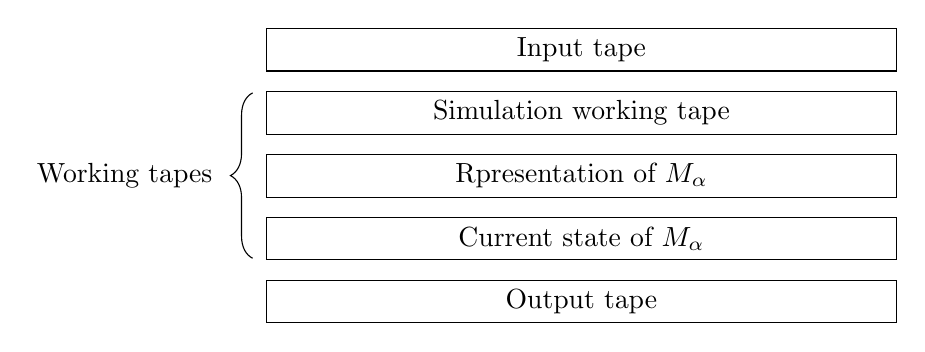
\begin{tikzpicture}
            \node[rectangle, draw, minimum width=8cm, minimum height=0.5 cm] (t1) at (0, 3.2) {Input tape};
            \node[rectangle, draw, minimum width=8cm, minimum height=0.5 cm] (t2) at (0, 2.4) {Simulation working tape};
            \node[rectangle, draw, minimum width=8cm, minimum height=0.5 cm] (t3) at (0, 1.6) {Rpresentation of $M_{\alpha}$};
            \node[rectangle, draw, minimum width=8cm, minimum height=0.5 cm] (t4) at (0, 0.8) {Current state of $M_{\alpha}$};
            \node[rectangle, draw, minimum width=8cm, minimum height=0.5 cm] (t5) at (0, 0.0) {Output tape};

            \draw[decorate, decoration={brace, raise=5pt, amplitude=8pt}] (-4, 0.55) -- (-4, 2.65) node[pos=0.5, left=16pt] {Working tapes};
        \end{tikzpicture}
        \caption{Universal Turing Machine}
        \label{fig:universal-turing-machine}
    \end{figure}
\end{proof}

\begin{rmk}
    In fact, the time bound can be improved using a more complicated encoding $\alpha$, such that if $M_{\alpha}$ halts on input $x$ within $T$ steps, then $U(x, \alpha)$ halts within $C_{\alpha}T\ln(T)$ steps for some $C_{\alpha} \in \N$.
\end{rmk}

\begin{thm}
    There exists a language that is not Turing recognizable.
\end{thm}

\begin{proof}
    Let $A$ be the set of all Turing machines, and let $L$ be the set of all languages. Since we can encode any Turing machine as a finite binary string, we can construct a bijection between the countably infinite set of finite binary strings, and $A$. Therefore $A$ is countable.

    Now, we prove that $L$ is uncountable. Consider the set $F$ of all functions from $\{0, 1\}^{*} \to \{0, 1\}$. We know that there is a bijection between $F$ and $L$, since any language can be uniquely represented as $f \in F$ such that for any finite binary string $w$, $f(w) = 1$ if and only if $w \in L$. Additionally, there is a bijection between $F$ and $[0, 1] \subset \R$. This is given by $f \in F \mapsto 0.f(w_0)f(w_1)\cdots f(w_n)\cdots \in [0, 1]$, where $w_0 = \emptystring$, $w_1 = 0$, $w_2 = 1$, $w_3 = 00$, etcetera. If $f_1 \mapsto r$ and $f_2 \mapsto r$, then $f_1(w) = f_2(w)$ for all finite binary strings $w$, and so $f_1 = f_2$. Furthermore, for any number $r \in [0, 1]$ we can explicitly construct $f$ from $r$. The necessary bijection between $[0, 1]$ and the set $T$ of all infinite binary strings, as well as the uncountability of $[0, 1]$ follows from Cantor's Diagonal Argument \ref{reals-uncountable}. We can then compose the bijections between $L$ and $F$, $F$ and $T$, and $T$ and $[0, 1]$ to obtain a bijection between $L$ and $[0, 1]$. Since $[0, 1]$ is uncountable, it follows that $L$ is as well.

    For any Turing machine $M \in A$, consider the language of all strings it recognizes. Since $A$ is countable but $L$ is not, this mapping cannot be surjective and so there exists a language that is not recognized by any Turing machine.
\end{proof}

\begin{lemma}\label{halting-lemma}
    For any $\alpha \in \{0, 1\}^{*}$, let $M_{\alpha}$ be the Turing machine encoded by $\alpha$. Define a Boolean function $UC$ such that $UC(\alpha) = 0$ if $M_{\alpha}$ accpts input $\alpha$, and $UC(\alpha) = 1$ otherwise (rejects or never halts). Let $L(UC)$ be the language of all strings $w$ such that $UC(w) = 1$.

    Then $L(UC)$ is not Turing recognizable.
\end{lemma}

\begin{proof}
    Assume, for the sake of contradiction, that $L(UC)$ is recognized by a Turing machine $M$ with encoding $\alpha$. Then $UC(\alpha) = 1$ if and only if $M$ accepts $\alpha$. However, $UC(\alpha)$ is defined to be $0$ if $M$ accepts. Therefore, $M$ can neither accept nor reject nor not halt on $\alpha$, and so no such $M$ exists.
\end{proof}

\begin{thm}\label{halting-problem}
    Let \verb|HALT| be the language consisting of all $\langle \alpha, x \rangle$ such that $M_{\alpha}$ halts on input $x$. Here, $\langle \alpha, x \rangle$ uses an encoding $\alpha$ for $M_{\alpha}$ such that a Turing machine can easily check if the input string begins with a valid encoding.

    Then \verb|HALT| is not Turing decidable.
\end{thm}

\begin{proof}
    Assume, for the sake of contradiction, that \verb|HALT| is Turing decidable by a Turing machine $M$ with encoding $\alpha$. Then construct the function $UC$ as follows: for given $\alpha$, use $M$ to determine if $M_{\alpha}$ will halt on input $\alpha$. If not, define $UC(\alpha) = 1$. If it does halt, simulate $\alpha$ until it halts, and define $UC(\alpha) = 0$ if it accepts and $UC(\alpha) = 1$ otherwise. Since we can simulate $\alpha$ using a Turing machine, this would allow use to construct a Turing machine that recognizes $L(UC)$ (in fact, decides it). However, this is a contradiction by Lemma \ref{halting-lemma}, and so \verb|HALT| cannot be decidable.
\end{proof}

\begin{rmk}
    This theorem essentially states no computable algorithm exists which can determine whether a Turing machine will halt on a given input, for all possible inputs and Turing machines. Such an algorithm may exist for some Turing machines and some inputs, but no such algorithm is universal.
\end{rmk}

\begin{prop}
    Let $A_{TM}$ be the language consisting of all $\langle M, \alpha \rangle$ such $M$ accepts $\alpha$. Then $A_{TM}$ is not decidable.
\end{prop}

\begin{proof}
    Assume, for the sake of contradiction, that there exists a Turing machine $M$ that decides $A_{TM}$. Define $UC(\alpha)$ to be $0$ if $M_{\alpha}$ accepts $\alpha$ and $1$ otherwise. We could then trivially compute this using $M$, which contradicts Lemma \ref{halting-lemma}.
\end{proof}

\begin{defn}
    A function $f$ $\Sigma^{*} \to \Sigma^{*}$ is \emph{computable} when there exists a Turing machine $M$ such that for any $w \in \Sigma^{*}$, $M$ will halt with its tape containing $f(w)$.
\end{defn}

\begin{defn}
    Consider languages $A$ and $B$. A \emph{mapping reduction} from $A$ to $B$ is a computable function $f: \Sigma^{*} \to \Sigma^{*}$ such that for any $w \in \Sigma^{*}$, $w \in A \iff f(w) \in B$. If a mapping reduction exists, we write $A \leq_{m} B$ and say that $A$ is \emph{mapping reducible} to $B$.
\end{defn}

\begin{thm}\label{mapping-reduction-decidability}
    Consider languages $A$ and $B$ such that $A \leq_m B$. If $B$ is decidable, then $A$ is decidable.
\end{thm}

\begin{proof}
    Let $M_1$ be a Turing machine which computes the reduction from $A$ to $B$. If $B$ is decided by a Turing machine $M_2$, then $M_2 \odot M_1$ is a Turing machine which decides $A$, so $A$ is decidable.
\end{proof}

\begin{thm}
    $A$ is decidable if and only if $A$ and $\complementof{A}$ are both Turing recognizable.
\end{thm}

\begin{proof}
    If $A$ and $\complementof{A}$ are recognized by Turing machines $M_1$ and $M_2$, we can construct a Turing machine $M$ which alternates running steps of $M_1$ and $M_2$ on separate tapes. If $w \in A$, then $M_1$ will accept, so $M$ accepts. If $w \not\in A$, then $w \in \complementof{A}$ so $M_2$ accepts and $M$ rejects. Therefore, $M$ decides $A$.

    If $A$ is decided by a Turing machine $M$, then $A$ is trivially recognizable. Let $M'$ reject when $M$ accepts and accept when $M$ rejects, and be identical otherwise. Then $M'$ decides $\complementof{A}$.
\end{proof}

\begin{exmp}
    Consider $E_{\textrm{TM}} = \left\{\langle M \rangle : L(M) = \emptyset\right\}$. Notice that the mapping $\langle M, \alpha \rangle \mapsto \langle M \rangle$ is \emph{almost} a mapping reduction from $A_{\textrm{TM}}$ to $\complementof{E_{\textrm{TM}}}$. We just neeed to tweak it slightly so that if $M$ does not accept $\alpha$ then $L(M) = \emptyset$. So define $f(\langle M, \alpha \rangle)$ to be the Turing machine that accepts $\alpha$ if and only if $M$ accepts $\alpha$, and rejects all other inputs. Then clearly $f(\langle M, \alpha \rangle) \in \complementof{E_{\textrm{TM}}}$ if and only if $\langle  M, \alpha \rangle \in A_{\textrm{TM}}$, so $f$ is a mapping reduction from $A_{\textrm{TM}}$ to $\complementof{E_{\textrm{TM}}}$.

    Since $A_{\textrm{TM}}$ is undecidable it follows that $\complementof{E_{\textrm{TM}}}$ is undecidable by Theorem \ref{mapping-reduction-decidability}, and therefore $E_{\textrm{TM}}$ is undecidable.
\end{exmp}

\begin{exmp}
    Consider $R_{\textrm{TM}} = \left\{\langle M \rangle : L(M) \textrm{ is a regular language}\right\}$. Consider $f(\langle M, \alpha \rangle) = M'$, where on input $\beta$, $M'$ runs $M$ on $\alpha$. If $M$ accepts $\alpha$, $M'$ accepts $\beta$ if it is a palindrome, and rejects otherwise. If $M$ rejects $\alpha$, $M'$ rejects all inputs. Therefore, if $\alpha \not\in L(M)$ then $L(M') = \emptyset$ (even if $M$ nevers halts since then neither does $M'$), and if $\alpha \in L(M)$ then $L(M')$ is the non-regular language of palindromes. It follows that $L(M')$ is regular if and only if $\alpha \not\in L(M)$. Therefore, we have a mapping reduction from $A_{\textrm{TM}}$ to the complement of $R_{\textrm{TM}}$, and so $R_{\textrm{TM}}$ is indeed undecidable.
\end{exmp}

\begin{defn}
    A \emph{non-deterministic} Turing machine uses a non-deterministic finite automaton as the control automaton. A non-deterministic Turing machine accepts an input if there exists a sequence of valid transitions for that machine that ends with the accept state, and rejects if all possible such sequences end with the reject state.
\end{defn}

\begin{defn}
    Let $N$ be a non-deterministic Turing machine. We say $N$ runs in time $f(n)$ if every valid sequence of transitions for any input of length $n$ has at most $f(n)$ transitions.
\end{defn}

\section{Complexity theory}

\begin{defn}
    \verb|DTIME|
\end{defn}

\begin{defn}
    Class P
\end{defn}

\begin{defn}
    Class NP
\end{defn}

\begin{exmp}
    Consider the language of strings $\langle G, k \rangle$ such that $G$ is an (encoding of) a graph with an independent set of size $k$. This language is in $NP$, since a list of $k$ vertices forming an independent set can be easily verified in polynomial time.
\end{exmp}

\begin{thm}
    \begin{align*}
        P \subseteq &NP \subseteq EXP \\
        P \subsetneq &EXP
    \end{align*}
\end{thm}

\begin{defn}
    $NP_2$ using non-deterministic Turing machines.
\end{defn}

\begin{thm}
    $NP = NP_2$
\end{thm}

\begin{defn}
    A language $A$ is \emph{polynomial-time reducible} to a language $B$ is there exists a mapping reduction of $A$ to $B$ using a function which is computable in polynomial time, written $A \leq_{p} B$.
\end{defn}

\begin{prop}
    If $L$ is polynomial-time reducible to $L'$, and $L' \leq_{p} L''$, then $L \leq_{p} L''$.
\end{prop}

\begin{defn}
    NP-hard is the class of languages $L$ such that any language in NP is polynomial-time reducible to $L$.
\end{defn}

\begin{defn}
    A language is NP-complete if it is both NP-hard and in NP.
\end{defn}

\begin{thm}\proofbreak
    \begin{itemize}
        \item If $L$ is in NP-hard and in P, then $P = NP$.
        \item If $L$ is NP-complete, then $L \in P$ if and only if $P = NP$.
    \end{itemize}
\end{thm}

\begin{defn}
    A Boolean formula with literals (Boolean variables) $x_1, \ldots, x_n $ is \emph{satisfied} by an \emph{assignment} of truth values $z_1, \ldots, z_n$ to its literals if it evaluates to \textsc{true}. A Boolean formula is \emph{satisfiable} if there exists an assignment which satisfies it.
\end{defn}

\begin{defn}
    A Boolean formula is in \emph{conjunctive normal form} (CNF) if it is a conjunction of one or more disjunctions of one or more literals or negation of literals. In other words, it is an \verb|AND| of \verb|OR|s.

    A Boolean formula is in \emph{disjunctive normal form} (DNF) if it is a disjunction of one or more conjunctions of one or more literals or negation of literals. In other words, it is an \verb|OR| of \verb|AND|s.

    The size of a formula is the sum of the length of clauses, where the length of a clause is the number of literals.
\end{defn}

\begin{lemma}\label{function-to-cnf}
    We can express any Boolean function $f: \{0, 1\}^{\ell} \to \{0, 1\}$ as a $\ell$ variable formula in CNF with at most $\ell 2^{\ell}$ clauses.
\end{lemma}

\begin{proof}
    Let $f: \{0, 1\}^{\ell} \to \{0, 1\}$. We will express this as a CNF formula with literals $x_1, \ldots, x_{\ell}$, where the string $x_1x_2\cdots x_{\ell}$ is the input to $f$. Let $A$ be the set of all strings $\omega$ such that $f(\omega) = 0$.

    For any $\omega = \omega_1\ldots \omega_{\ell} \in A$, let $a_i = x_i$ if $\omega_i = 0$ and $a_i = \neq x_i$ if $\omega_i = 1$. Consider the clause $a_1 \lor a_2 \lor \cdots \lor a_{\ell}$. If this clause is true, then $x_1\ldots x_{\ell}$ must differ from $\omega$ in at least one position. Since $|A| \leq 2^{\ell}$, we can enumerate all such clauses as $c_1, \ldots, c_{k}$ where $k \leq 2^{\ell}$. Then the CNF formula
    \begin{align*}
        c_1 \land c_2 \land \cdots \land c_{k}
    \end{align*}
    is equivalent to $f(\omega)$, since it is true precisely when $\omega \not\in A$.

    Note that every clause contains exactly $\ell$ literals, and there are $k \leq 2^{\ell}$ clauses. Therefore, the overall formula has size at most $\ell 2^{\ell}$.
\end{proof}

\begin{defn}
    SAT is the language of all satisfiable CNF Boolean formulas. 3-SAT is the language of all satisfiable CNF Boolean formulas, where each clause has length at most three.
\end{defn}

\begin{lemma}\label{CNF-to-3-CNF}
    Let $X$ be a CNF formula with size $n$, then there exists a 3-CNF formula which is satisfiable if and only if $X$ is satisfiable, and whose size is polynomial in $n$.
\end{lemma}

\begin{proof}
    Consider any clause $x_1 \lor x_2 \lor x_3 \lor \cdots \lor x_n$. Notice that this is equivalent to $(x_1 \lor x_2 \lor y) \land (\neq y \lor x_3 \lor \cdots \lor x_n)$, which has two clauses of size three and $n-1$. Therefore, we can recursively reduce $X$ to a 3-CNF formula by breaking apart every clause with length longer than three. Every clause of length $k > 3$ is reduced to a 3-CNF formula of size $3(k-3) + 3 = 3(k-2)$. Therefore, a CNF formula $X$ of size $n$ can be reduced to a formula of size at most $3(n-2)$, since the worst case occurs when $X$ contains a single clause of length $n$.
\end{proof}

\begin{thm}{Cook-Levin theorem}\proofbreak
    Both SAT and 3-SAT are NP-complete.
\end{thm}

\begin{proof}
    SAT and 3-SAT are in NP, because a certificate consisting of an assignment of the variables can be easily verified in polynomial time.

    For any language $L$ in NP, by definition there exists a polynomial function $p: \N \to \N$ and polynomial time Turing machine $M$ such that $x \in \{0, 1\}^{*}$ is in $L$ if and only if there exists $u$ of length at most $p(\abs{x})$ such that $M(x, u) = 1$. Note that for fixed $x$, $M(x, u)$ is equivalent to $M'(u)$ for some $M'$, and is therefore equivalent to $\phi(u)$ for some binary function $\phi$. By Lemma \ref{function-to-cnf}, $\phi$ can be expressed as a CNF formula, however this is not necessarily computable in polynomial time since the formula can have size $|x|2^{|x|}$.

    Consider the following polynomial-time computable construction of a CNF formula from the Turing machine $M$. We know that $M(x, u) = 1$ if and only if there exists a sequence of configurations $C_0, \ldots, C_t$ such that $C_0$ is the start configurtion, $C_T$ is an accept configuration, and $C_i \to C_{i+1}$ obeys the transition function. Note that $T$ is bounded by the running time of $M$, which is polynomial. For all $C_i$, let $z_i$ be a set of Boolean variables describing the $C_i$, including head positions, control automaton state, and tape states, and let $u_1, \ldots, u_k$ such that $u = u_1\cdots u_k$ is the certificate. Since the tapes of $C_i$ and $C_{i+1}$ can only differ in a single window of length three around the head position, we can verify a transition by checking that all but one window remains the same, and the window which changes obeys the transition function.

    The full details are exceedingly complex, see the Cook-Levin Theorem in Chapter 7 of Sipser's ``Introduction to the Theory of Computation'', 3rd edition, for some of these details. Essentially, a CNF formula can be constructed in polynomial time that states whether a series of configurations is equivalent to the computation of $M(x, u)$, where $M(x, u)$ accepts. Therefore, the satisfiability of this CNF problem is equivalent to deciding $x$, and since it is done with a polynomial-time reduction, SAT is NP-hard by definition, and therefore NP-complete.

    Finally, we show that SAT is polynomial-time reducible to 3-SAT. By Lemma \ref{CNF-to-3-CNF}, we can compute in polynomial-time a reduction of any CNF formula to a 3-CNF formula, and so $SAT \leq_{p} 3-SAT$, so $3-SAT$ is NP-hard.
\end{proof}

\setchaptergraphic{}

\chapter{Group Theory}
\label{ch:groups}

\section{Symmetries}

Our first motivation for studying groups will be the symmetries of regular $n$-gons, starting with the regular $3$-gon: the equilateral triangle. The symmetries of a regular $n$-gon in the plane are rotations and reflections which take the $n$-gon to itself.

For example, if we take an equilateral triangle and label the vertices $A, B, C$, in anti-clockwise order starting from the top, we have two rotational symmetries: rotation by $120^\circ$ and rotation by $240^\circ$, in a particular sense or direction, say anti-clockwise. We also have three reflection symmetries --- reflections across a line going from one vertex to the midpoint of the opposite edge.

\begin{figure}[ht!]
    \centering
    \begin{tikzpicture}
        \coordinate (A1) at (0, {sqrt(3)});
        \coordinate (B1) at (-1, 0);
        \coordinate (C1) at (1, 0);
        \coordinate (R1) at ($(B1)!0.5!(C1)$);
        \coordinate (R11) at ($(A1)!1.25!(R1)$);
        \coordinate (R12) at ($(R1)!1.25!(A1)$);

        \node[anchor=south east] at (A1) {$A$};
        \node[anchor=east] at (B1) {$B$};
        \node[anchor=west] at (C1) {$C$};

        \draw [thick] (A1)--(B1);
        \draw [thick] (B1)--(C1);
        \draw [thick] (C1)--(A1);

        \draw [thick, dashed] (R11)--(R12);

        \coordinate (A2) at (4, {sqrt(3)});
        \coordinate (B2) at (5, 0);
        \coordinate (C2) at (3, 0);
        \coordinate (R2) at ($(B2)!0.5!(C2)$);
        \coordinate (R21) at ($(A2)!1.25!(R2)$);
        \coordinate (R22) at ($(R2)!1.25!(A2)$);

        \node[anchor=south east] at (A2) {$A$};
        \node[anchor=west] at (B2) {$B$};
        \node[anchor=east] at (C2) {$C$};

        \draw [thick] (A2)--(B2);
        \draw [thick] (B2)--(C2);
        \draw [thick] (C2)--(A2);

        \draw [thick, dashed] (R21)--(R22);
    \end{tikzpicture}
\caption{Reflection symmetry $S_1$}
\label{fig:triangle-reflection}
\end{figure}

Let $R$ be the rotation by $120^\circ$ anti-clockwise. Then the rotation by $240^\circ$ anti-clockwise is simply $R$ applied twice, so we will denote it by $R^2$. Let $S_1$ be the reflection symmetry across the line through the top vertex, $S_2$ across the line through the left vertex, and $S_2$ the right vertex. The final symmetry is the identity transform, which we will call $e$. The triangle therefore has six symmetries in total: $\{e, S_1, S_2, R, R^2\}$.

\begin{figure}[ht!]
    \centering
    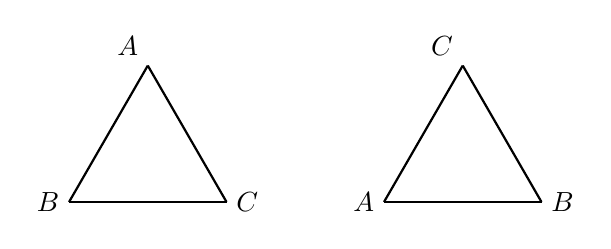
\begin{tikzpicture}
        \coordinate (A1) at (0, {sqrt(3)});
        \coordinate (B1) at (-1, 0);
        \coordinate (C1) at (1, 0);

        \node[anchor=south east] at (A1) {$A$};
        \node[anchor=east] at (B1) {$B$};
        \node[anchor=west] at (C1) {$C$};

        \draw [thick] (A1)--(B1);
        \draw [thick] (B1)--(C1);
        \draw [thick] (C1)--(A1);

        \coordinate (A2) at (3, 0);
        \coordinate (B2) at (5, 0);
        \coordinate (C2) at (4, {sqrt(3)});

        \node[anchor=east] at (A2) {$A$};
        \node[anchor=west] at (B2) {$B$};
        \node[anchor=south east] at (C2) {$C$};

        \draw [thick] (A2)--(B2);
        \draw [thick] (B2)--(C2);
        \draw [thick] (C2)--(A2);
    \end{tikzpicture}
\caption{Rotation symmetry $R$}
\label{fig:triangle-rotation}
\end{figure}

Since every symmetry takes the triangle to itself, products (compositions) of Symmetries are themselves symmetries. If $u$ and $w$ are symmetries, let $uw$ denote the composition of first $w$ and then $u$ after the manner of function composition. For example, $S_1S_2 = R$, $RR = R^2$, and $R^2R = e$.

Note that multiplication of symmetries is not necessarily commutative: $S_1S_2 = R$, but $S_2S_1 = R^2$. Multiplication with the identity is however commutative: $eR^2 = R^2 = R^2e$, etc.

We can construct a full multiplication table for the six symmetries of the $3$-gon listing all possible binary products, which is shown in Table \ref{triangle-multiplication-table}.

\begin{minipage}{\linewidth}
    \begin{center}
    \captionof{table}{Group multiplication table for $3$-gon}
    \label{triangle-multiplication-table}
    \begin{tabular}{|c||c|c|c|c|c|c|}
    \hline
    \thead{$\circ$} & \thead{$e$} & \thead{$S_1$} & \thead{$S_2$} & \thead{$S_3$} & \thead{$R$} & \thead{$R^2$}\\
    \hline\hline
    $e$   & $e$   & $S_1$ & $S_2$ & $S_3$ & $R$   & $R^2$ \\ \hline
    $S_1$ & $S_1$ & $e$   & $R$   & $R^2$ & $S_2$ & $S_3$ \\ \hline
    $S_2$ & $S_2$ & $R^2$ & $e$   & $R$   & $S_3$ & $S_1$ \\ \hline
    $S_3$ & $S_3$ & $R$   & $R^2$ & $e$   & $S_1$ & $S_2$ \\ \hline
    $R$   & $R$   & $S_3$ & $S_1$   & $S_2$ & $R^2$ & $e$   \\ \hline
    $R^2$ & $R^2$ & $S_2$ & $S_3$ & $S_1$ & $e$   & $R$   \\ \hline
    \end{tabular}
    \end{center}
\end{minipage}

\section{Group Axioms}

\begin{defn}
    A \emph{group} $G$ is a set together with a closed binary operation on the elements of the set (typically called ``multiplication'') that satisfies the following axioms:
    \begin{itemize}
        \item There exists an identity element $e \in G$ such that $ex = x = xe$ for every $x \in G$.
        \item Every element $x \in G$ has an inverse $x^{-1}$ such that $xx^{-1} = e$.
        \item The operation is associative: $x(yz) = (xy)z$, for every $x, y, z \in G$.
    \end{itemize}
\end{defn}

\begin{exmp}
    The symmetries of a triangle $\{e, S_1, S_2, S_3, R, R^2\}$, together with the binary operation of composition, form a group. Table \ref{triangle-multiplication-table} shows that every element has an inverse and that composition of these symmetries is closed. Associativity comes from the fact that $(xy)z$ means apply the symmetry $z$, then $y$, and then $x$, and $x(yz)$ also means apply $z$, then $y$, and then $x$, so the result is the same and $(xy)z = x(yz)$.
\end{exmp}

\begin{exmp}
    $\N$, $\Z$, $\Q$, $\R$, and $\C$ all form groups under addition, and $\Q - \{0\}$, $\R - \{0\}$, and $\C - \{0\}$ form groups under multiplication.
\end{exmp}

\begin{exmp}
    $\{1, -1, i, -i\} \subset \C$ forms a group under complex multiplication. It can be easily verified it is closed under multiplication, $1$ is the identity, and it inherits associativity from $\C$. Inverse can be easily checked: $(-1)(-1) = 1$ and $i(-i) = 1$.
\end{exmp}

\begin{defn}
    If a group is commutative, then it is an \emph{abelian} group.
\end{defn}

\begin{defn}
    The \emph{order} of a group is the cardinality of the group.
\end{defn}

\begin{defn}
    A \emph{subgroup} $H$ of a group $G$ is a set $H \subseteq G$ that forms a group under the same group operation as $G$. If $H$ is a subgroup of $G$ this may be denoted by $H \leqslant G$, or $H < G$ if it is a strict subgroup.
\end{defn}

\begin{thm}\label{subgroup-test}
    A non-empty subset $H$ of a group $G$ is a subgroup of $G$ if and only if $x, y \in H$ implies $xy^{-1} \in H$.
\end{thm}

\begin{proof}\proofbreak
    ($\implies$) If $H$ is a subgroup of $G$, then since $y \in H$ it must be that $y^{-1} \in H$. Since groups are closed under the group operation, $x, y^{-1} \in H$ then implies that $xy^{-1} \in H$.

    ($\impliedby$) Since $H$ is non-empty, there must exist some $x \in H$, and so $xx^{-1} \in H$, which implies $H$ contains the identity. $H$ clearly inherits associativity from $G$, so it only remains to check that it contains inverses and is closed. Since $e, x \in H$, $ex^{-1} \in H$, but $ex^{-1} = x^{-1}$ so $H$ contains all inverses. Finally, if $x, y \in H$, we also have $x, y^{-1} \in H$, so $xy \in H$ and so $H$ is closed.
\end{proof}

\begin{thm}
    Let $H, K \subseteq G$ be subgroups. Then $H \intersection K$ is a subgroup of $G$.
\end{thm}

\begin{proof}
    Since $e \in H$ and $e \in K$, we of course have $e \in H \intersection K$. If $x \in H \intersection K$, then $x^{-1} \in H$ and $x^{-1} \in K$ so $x \in H \intersection K$. If $x, y \in H \intersection K$, then $xy \in H$ and $xy \in K$ so $xy \in H \intersection K$. Finally, $H \intersection K$ inherits associativity from $G$, so it is a subgroup.
\end{proof}

\section{Cyclic Groups}

\begin{defn}
    Let $G$ be a group, where $e \in G$ is the identity. For any $x \in G$, we define $x^0 = e$, and for $n \in \Z^+$ we define $x^n = x^{n-1}$. Finally, we define $x^{-n} = \left(x^n\right)^{-1}$.
\end{defn}

\begin{defn}
    Let $G$ be a group. If there exists some $x \in G$ such that for every $y \in G$ we have $y = x^n$ for some $n \in \Z$, then we say that $G$ is \emph{cyclic}, and that $x$ \emph{generates} $G$.
\end{defn}

\begin{defn}
    Let $G$ be a group. If there exists some $x_1, x_2, \ldots, x_k \in G$ such that for every $y \in G$ we have $y = x_1^{a_1}x_2^{a_2}{\cdots}x_k^{a_k}$ for some $a_1, a_2, \ldots, a_k \in \Z$, then we say that $G$ is generated by $\{x_1, x_2, \ldots, x_k\}$, and that $\{x_1, x_2, \ldots, x_k\}$ \emph{generates} $G$.
\end{defn}

\begin{defn}
    Let $G$ be a group, and $x$ be an element of $G$. The set of all elements of $G$ generated by $x$ may be denoted by $\langle{x}\rangle$.
\end{defn}

\begin{prop}
    Let $G$ be a group, and $x \in G$. Then $\langle{x}\rangle$ is a subgroup of $G$.
\end{prop}

\begin{proof}
    Given $x^n, x^m \in \langle{x}\rangle$, $x^nx^m = x^{n+m} \in \langle{x}\rangle$, so $\langle{x}\rangle$ is closed.

    Since $x^0 = e$, it has the identity, and since for any $x^n$ we have $x^{-n}$, and $x^{-n}x^n = x^0 = e$, $\left(x^n\right)^{-1} \in \langle{x}\rangle$. Finally, $\langle{x}\rangle$ inherits associativity from $G$.
\end{proof}

\begin{defn}
    The \emph{order} of an element $x$ is the order of $\langle{x}\rangle$.
\end{defn}

\begin{prop}
    Let $G$ be a group. Then for any $x \in G$, $x^n = e$ if and only if $x$ has finite order $n$.
\end{prop}

\begin{proof}\proofbreak
    ($\implies$) If $x^n = e$, then for any $k = qn + r$ where $q, r \in \Z$ and $0 \leq r < n$, we know $x^k = (x^n)^qx^r = e^qx^r = x^r$, so any element $x^k \in \langle{x}\rangle$ is one of $\{x^0, x^1, \ldots, x^{n-1}\}$. It follows that the order of $x$ is $n$.

    ($\impliedby$) If $\langle{x}\rangle$ has order $n$, then it is equal to $\{x^0, x^1, \ldots, x^{n-1}\}$. Since every element has an inverse, there is some $m \leq n-1$ such that $x^1x^m = x^0 = e$, so $x^{m+1} = e$. If $m+1 < n$, then $\langle{x}\rangle$ would have order less than $n$, which is false, so $m+1 = n$, and so $x^n = e$.
\end{proof}

\begin{cor}
    Since $x^n = e$, it follows that $\left(x^m\right)^{-1} = x^{n-m}$.
\end{cor}

\begin{exmp}
    $\Z$ is cyclic, and is generated by $1$ since $n = 1 \cdot n$, as well as by $-1$.
\end{exmp}

\begin{rmk}
    If $G$ is a cyclic group that is generated by $x \in G$, then $G$ is also generated by $x^{-1}$.
\end{rmk}

\begin{exmp}
    $\Z/n\Z$ is a \emph{finite} cyclic group, and is generated by $1$ and $n-1$ (since $1^{-1} = n-1$).
\end{exmp}

\begin{prop}
    All cyclic groups are abelian.
\end{prop}

\begin{proof}
    Let $G$ be a cyclic group, and $m \in G$ such that $m$ generates $G$. Now consider any $x, y \in G$. We know that there exists some $n_1, n_2 \in \Z$ such that $x = m^{n_1}$ and $y = m^{n_2}$, so $xy = m^{n_1}m^{n_2} = m^{n_1 + n_2} = m^{n_2}m^{n_1} = yx$.
\end{proof}

\begin{lemma}\label{cyclic-subgroups-of-z}
    All subgroups of $\Z$ are cyclic.
\end{lemma}

\begin{proof}
    Let $H$ be a subgroup of $\Z$. If $H = \{0\}$, then $H$ is trivially cyclic, so assume $H \neq \{0\}$. For any $x \in H$, $-x$ must also be in $H$, and so since $H \neq \{0\}$ there must be some smallest positive integer $m$ in $H$.

    Now consider any $k \in H$. We know that $k = qm + r$ for some $q \in \Z$ and $0 \leq r < m$ --- that is, $r = k \bmod m$ and $q = \frac{k - r}{m}$. Since $m, k \in H$, and $r = k + (-qm)$, we know that $r \in H$. Since $m$ is the smallest positive integer in $H$, it follows that $r = 0$. Therefore, $k = qm$, so $m$ generates all of $H$, and it follows that $H$ must be cyclic.
\end{proof}

\begin{thm}
    Let $G$ be a cyclic group, and $H$ a subgroup of $G$. Then $H$ is itself cyclic.
\end{thm}

\begin{proof}
    Let $x$ be any generating element of $G$. We know that for any $y \in H$, there exists some $n \in \Z$ such that $y = x^n$. Consider \[K = \left\{n \in \Z \compbar x^n \in H\right\}.\] We can show that $K$ is a subgroup of $\Z$: if $n_1, n_2 \in K$, then $x^{n_1}x^{n_2} = x^{n_1 + n_2} \in H$, so $n_1 + n_2 \in K$, so $K$ is closed. Since $x^0 \in H$, $K$ has the identity, and since $x^{-n} \in H$, we have $n \in K$ for any $n \in K$. Finally, $K$ inherits associativity from $\Z$. By Lemma \ref{cyclic-subgroups-of-z}, it follows that $K$ is cyclic.

    Since $K$ is cyclic, it is generated by some $m \in K$. Therefore, every $y \in H$ can be expressed as $x^{qm}$ for some $q \in \Z$, and so $y = (x^m)^q$. It follows that $H$ is generated by $x^m$, and so $H$ is cyclic.
\end{proof}

\section{Permutations}

\begin{defn}
    Let $X$ be a set, and let $S_X$ be the set of all bijections from $X$ to itself. These bijections are called \emph{permutations} of $X$.
\end{defn}

\begin{prop}\label{permutations-group}
    For a given set $X$, $S_X$ is a group.
\end{prop}

\begin{proof}
    Composition of bijections is of course a bijection, so $S_X$ is closed. Since the inverse of a bijection is also a bijection, $S_X$ has inverses, and of course the identity function is then the identity of $S_X$. Finally, composition of functions is associative so $S_X$ is a group.
\end{proof}

\begin{defn}
    For $n \in Z^+$, the finite \emph{symmetric group} $S_n$ is the group $S_X$ where $X = \{1, 2, \ldots, n\}$.
\end{defn}

\begin{rmk}
    $S_n$ has order $n!$.
\end{rmk}

\begin{rmk}
    We may denote permutations in the form
    $\begin{bmatrix}
        a & b & c \\ c & b & a
    \end{bmatrix}$, meaning $a$ is sent to $c$, $b$ is sent to $b$, and $c$ is sent to $a$.
\end{rmk}

\begin{exmp}
    \[S_3 = \left\{
        \begin{bmatrix}
            1 & 2 & 3 \\ 1 & 2 & 3
        \end{bmatrix},
        \begin{bmatrix}
            1 & 2 & 3 \\ 1 & 3 & 2
        \end{bmatrix},
        \begin{bmatrix}
            1 & 2 & 3 \\ 2 & 1 & 3
        \end{bmatrix},
        \begin{bmatrix}
            1 & 2 & 3 \\ 2 & 3 & 1
        \end{bmatrix},
        \begin{bmatrix}
            1 & 2 & 3 \\ 3 & 1 & 2
        \end{bmatrix},
        \begin{bmatrix}
            1 & 2 & 3 \\ 3 & 2 & 1
        \end{bmatrix}
    \right\}\]

    The composition
    \[\begin{bmatrix}
        1 & 2 & 3 \\ 2 & 3 & 1
    \end{bmatrix}
    \begin{bmatrix}
        1 & 2 & 3 \\ 3 & 2 & 1
    \end{bmatrix}\] is read right to left, and so is equal to
    \[\begin{bmatrix}
        1 & 2 & 3 \\ 1 & 3 & 2
    \end{bmatrix}.\]
\end{exmp}

\begin{defn}
    The above notation for writing permutations is rather cumbersome, so \emph{cyclic notation} is commonly used. In this notation, we write $\begin{bmatrix}
        1 & 2 & 3 \\ 2 & 3 & 1
    \end{bmatrix}$ as $(123)$, meaning that $1$ is sent to $2$, $2$ is sent to $3$, and $3$ is sent back to $1$, ending the cycle. Every permutation can be written as the composition of a finite number of disjoint cycles.
\end{defn}

\begin{defn}
    A \emph{transposition} is a permutation which swaps two elements, leaving the others unchanged. It can therefore be written as $(ab)$ is cyclic notation, where $a$ and $b$ are the elements being swapped.
\end{defn}

\begin{thm}\label{transpositions-generate-sn}
    Let $X = \left\{(ab) \compbar a, b \in \{1, 2, \ldots, n\}\right\}$, the set of all transpositions in $S_n$. $S_n$ is generated by $X$.
\end{thm}

\begin{proof}
    Since any permutation in $S_n$ is the product of disjoint cycles, it is sufficient to show that any cycle is the product of (not necessarily disjoint) transpositions. Let $(a_1a_2\ldots a_k)$ be a cycle. Then
    \[(a_1a_k)(a_1a_{k-1})\cdots(a_1a_2) = (a_1a_2\ldots a_k).\]
\end{proof}

\begin{thm}\label{one-transpositions-generate-sn}
    Let $X = \left\{(1a) \compbar a \in \{1, 2, \ldots, n\}\right\}$, the set of all transpositions in $S_n$ which start with $1$. $S_n$ is generated by $X$.
\end{thm}

\begin{proof}
    By Theorem \ref{transpositions-generate-sn}, the set of transpositions in $S_n$ generate $S_n$, so we only need to show that the set of transpositions of the form $(1a) \in S_n$ can be used to create the set of transpositions in $S_n$.

    Let $(ab)$ be a transposition. If $a = 1$, it is already in the desired form. Otherwise, note that $(ab) = (1a)(1b)(1a)$.
\end{proof}

\begin{defn}
    Consider the polynomial in $\R$
    \[P = (x_1 - x_2)(x_1 - x_3)\cdots(x_1 - x_n)(x_2 - x_3)\cdots(x_{n-1} - x_n).\]
    For $\alpha \in S_n$, let $\alpha P$ denote the polynomial
    \[P = (x_{\alpha(1)} - x_{\alpha(2)})(x_{\alpha(1)} - x_{\alpha(3)})\cdots(x_{\alpha(1)} - x_{\alpha(n)})(x_{\alpha(2)} - x_{\alpha(3)})\cdots(x_{\alpha(n-1)} - x_{\alpha(n)}).\]
    Clearly $\alpha P = \pm P$. If $\alpha P = P$, we say that the sign of $P$ is $1$, and if $\alpha P = -P$ that the sign is $-1$.
\end{defn}

\begin{prop}\label{sign-product}
    If $\alpha, \beta \in S_n$, the sign of $\alpha\beta$ is the product of the signs of $\alpha$ and $\beta$.
\end{prop}

\begin{prop}
    The sign of any transposition is $-1$.
\end{prop}

\begin{proof}\label{transposition-sign-is-negative}
    The sign of $(12)$ is $-1$, since it changes $(x_1 - x_2)$ to $(x_2 - x_1)$ in $P$, and swaps $(x_1 - x_n)$ and $(x_2 - x_n)$. For $a > 2$, $(1a) = (2a)(12)(2a)$, so the sign of $(1a) = -1$. Since $(ab) = (1a)(1b)(1a)$, the sign of $(ab) = -1$.
\end{proof}

\begin{prop}
    If the sign of a permutation is $1$, it is the product of an even number of transpositions, and an odd number if the sign is $-1$.
\end{prop}

\begin{proof}
    Since the sign of any transposition is negative, by Proposition \ref{sign-product} if the sign of a permutation is $1$ it must be the product of an even number of transpositions, and an odd number if the sign is $-1$.
\end{proof}

\begin{defn}
    A permutation is called \emph{even} it is the product of an even number of transpositions (and thus has sign $1$), and \emph{odd} if the required number of transpositions is odd (and thus has sign $-1$).
\end{defn}

\begin{thm}
    The even permutations in $S_n$ form a subgroup of $S_n$ called $A_n$, the alternating group.
\end{thm}

\begin{exmp}
    $A_3 = \{e, (123), (132)\} \subset S_3$.
\end{exmp}

\begin{proof}
    Given permutations $a, b \in A_n$, their product can trivially be written as the concatenation of their transpositions, and so is even. Since $e$ is the product of $0$ transpositions, or $(12)(21)$, $e \in A_n$. For any $(a_1a_2\ldots a_k) \in A_n$, we know that $(a_1a_2\ldots a_k) = (a_1a_k)(a_1a_{k-1})\cdots(a_1a_2)$. Therefore, $(a_1a_2\ldots a_k)^{-1} = (a_1a_2)(a_1a_3)\cdots(a_1a_k)$, and so is in $A_n$. Finally, associativity is inherited from $S_n$.
\end{proof}

\begin{prop}
    The order of $A_n$ is $\frac{n!}{2}$, half that of $S_n$.
\end{prop}

\begin{proof}
    Consider the permutation $(1a) \in S_n$ for some $a \neq 1$. We know that $(1a) \not\in A_n$. Consider the function $f(k) = k(1a)$, where $k \in A_n$. We will show that $f$ is a bijection between the even and odd elements of $S_n$. Since $k$ is even and $(1a)$ is odd, $f(k)$ must be odd. Now consider $k_1, k_2 \in A_n$ such that $f(k_1) = f(k_2)$. Then $k_1(1a) = k_2(1a)$ so $k_1(1a)(1a) = k_2(1a)(1a)$, and so $k_1 = k_2$, proving $f$ is injective. Now consider any $y \not\in A_n$. Since $(1a)$ is odd, $y(1a)$ is even and must be in $A_n$. Therefore, $f(y(1a)) = y(1a)(1a) = y$, and so $f$ is also surjective. Since $f$ is a bijection between the even and odd elements of $S_n$, it follows that precisely half of the elements of $S_n$ are even.
\end{proof}

\section{Isomorphisms}

\begin{defn}
    An \emph{isomorphism} between two groups $G$ and $G'$ is a bijection $\varphi: G \to G'$ such that $\varphi(xy) = \varphi(x)\varphi(y)$ for all $x, y \in G$. If there is an isomorphism between $G$ and $G'$, we say that $G$ is \emph{isomorphic} to $G'$, written $G \cong G'$.
\end{defn}

\begin{prop}\label{isomorphism-inverse}
    If $\varphi: G \to G'$ is an isomorphism, then so is $\varphi^{-1}$.
\end{prop}

\begin{proof}
    Since $\varphi$ is a bijection, so is $\varphi^{-1}$. Therefore, for $x, y \in G$, it is sufficient to show that $\varphi(x) = \varphi(y)$ in order to prove that $x = y$. Consider $x', y' \in G'$. Then $\varphi\left(\varphi^{-1}(x'y')\right) = xy$, and $\varphi\left(\varphi^{-1}(x')\varphi^{-1}(y')\right) = \varphi\left(\varphi^{-1}(x')\right)\varphi\left(\varphi^{-1}(y')\right) = x'y'$. Therefore, $\varphi^{-1}(x'y') = \varphi^{-1}(x')\varphi^{-1}(y')$.
\end{proof}

\begin{rmk}
    If $G \cong G'$, then $\abs{G} = \abs{G'}$ since there is a bijection between them. But $\abs{G} = \abs{G'}$ doesn't imply $G \cong G'$ since there is no guarantee of an isomorphism.
\end{rmk}

\begin{prop}\label{isomorphism-preserves-identity-inverses}
    Let $\varphi$ be an isomorphism between $G$ and $G'$. Then $\varphi(e) = e$, and for $x \in G$, $\varphi(x^{-1}) = \varphi(x)^{-1}$.
\end{prop}

\begin{proof}
    For $x \in G$, we know $\varphi(x) = \varphi(ex) = \varphi(e)\varphi(x)$, so $\varphi(e)$ is a left identity in $G'$. Similarly, $\varphi(x) = \varphi(xe) = \varphi(x)\varphi(e)$, so $\varphi(e) = e$.

    Consider $\varphi(xx^{-1})$, which is $\varphi(x)\varphi(x^{-1})$. Since
    \[e = \varphi(e) = \varphi(xx^{-1}) = \varphi(x^{-1}x) = \varphi(x)\varphi(x^{-1}),\]
    we have $e = \varphi(x^{-1})\varphi(x)$ and so $\varphi(x^{-1}) = \varphi(x)^{-1}$.
\end{proof}

\begin{prop}\label{isomorphism-subgroups}
    Let $G, G'$ be groups where $\varphi: G \to G'$ is an isomorphism, and $H$ be a subgroup of $G$. Then $\varphi(H)$ is a subgroup of $G'$, and $H \cong \varphi(H)$.
\end{prop}

\begin{proof}
    Consider $x', y' \in \varphi(H)$. Then there exist $x, y \in H$ such that $x' = \varphi(x)$ and $y' = \varphi(y)$. Therefore, $\varphi(xy) = x'y' \in \varphi(H)$, so $\varphi(H)$ is closed under multiplication.

    Since $\varphi(e) = e$, $\varphi(e)$ contains the identity. Furthermore, given $x' \in \varphi(H)$, we know there is some $x \in H$ such that $\varphi(x) = x'$. By Proposition \ref{isomorphism-inverse}, $\varphi(x^{-1}) = \varphi(x)^{-1} = x'^{-1}$, so $\varphi(H)$ contains all inverses. Finally, $\varphi(H)$ inherits associativity from $G'$, so it is a subgroup of $G'$.
\end{proof}

\begin{prop}
    Let $G, G'$ be groups where $\varphi: G \to G'$ is an isomorphism. If $g \in G$ has order $n$, then $\varphi(g)$ also has order $n$.
\end{prop}

\begin{proof}
    Since $g$ has order $n$, we know that $g^n = e$. By Proposition \ref{isomorphism-preserves-identity-inverses}, it follows that $\varphi(g^n) = e$. Since $\varphi(g^n) = \varphi(g)\varphi(g^{n-1}) = \cdots = \varphi(g)^n$, it follows that the order of $\varphi(g)$ is less than or equal to $n$.

    Let $n'$ be the order of $\varphi(g)$. Since $\varphi(g)^{n'} = e$, we have $\varphi^{-1}(\varphi(g)^{n'}) = e$ by Proposition \ref{isomorphism-preserves-identity-inverses}. Then $\varphi^{-1}(\varphi(g)^{n'}) = \varphi^{-1}(\varphi(g))^{n'} = g^{n'} = e$, so the order of $g$ must be less than or equal to $n'$.

    We therefore have $n' \leq n$ and $n \leq n'$, so it follows that $n = n'$, and so $\varphi(g)$ has the same order as $g$.
\end{proof}

\begin{prop}\label{abelian-isomorphism}
    Let $G, G'$ be groups where $\varphi: G \to G'$ is an isomorphism, and let $G$ be abelian. Then $G'$ is also abelian.
\end{prop}

\begin{proof}
    Let $x, y \in G$. Then $\varphi(xy) = \varphi(x)\varphi(y)$, and $\varphi(yx) = \varphi(y)\varphi(x)$. Since $G$ is abelian, $\varphi(xy) = \varphi(yx)$, and so $\varphi(x)\varphi(y) = \varphi(y)\varphi(x)$. Since $\varphi$ is surjective, it follows that $G'$ is abelian.
\end{proof}

\begin{thm}\label{cyclic-isomorphism}\proofbreak
    \begin{itemize}
        \item Any infinite cyclic group is isomorphic to $\Z$.
        \item Any finite cyclic group of order $n$ is isomorphic to $\Z/n\Z$.
    \end{itemize}
\end{thm}

\begin{proof}
    Let $G_1$ be an infinite cyclic group, and $x \in G_1$ generate $G_1$. Then $\varphi: \Z \to G_1$ where $\varphi(n) = x^n$ is an isomorphism from $\Z$ to $G_1$.

    Let $G_2$ be a finite cyclic group of order $n$, and $x \in G_2$ generate $G_2$. Then $\varphi: \Z/n\Z \to G_2$ where $\varphi(m) = x^m$ is an isomorphism from $\Z/n\Z$ to $G_2$.
\end{proof}

\begin{exmp}
    Let $G = \left\{1, -1, i, -i\right\}$. Since $i^0 = 1$, $i^1 = i$, $i^2 = -1$, and $i^3 = -i$, it is a finite cyclic group of order four, and so is isomorphic to $\Z/4\Z$.
\end{exmp}

\begin{exmp}
    Let $G = \left(\R, +\right)$ and $G' = \left(\R^+, \times\right)$, and consider $\varphi: \R \to \R^+$ where $\varphi(x) = e^x$. Since $\varphi$ is a bijection, and $\varphi(x + y) = e^{x+y} = e^xe^y = \varphi(x)\varphi(y)$, $\varphi$ is an isomorphism, and so the real numbers under addition are isomorphic to the positive real numbers under multiplication.
\end{exmp}

\begin{defn}
    If $\varphi: G \to G'$ is an isomorphism, and $G = G'$, we say that $\varphi$ is an \emph{automorphism}.
\end{defn}

\begin{prop}
    Let $G$ be a group, and fix some $g_0 \in G$. Then $\varphi(g) = g_0 \cdot g \cdot g_0^{-1}$ is an automorphism.
\end{prop}

\begin{proof}
    First we need to show that $\varphi$ is a bijection. Consider some $g_1, g_2 \in G$ such that $\varphi(g_1) = \varphi(g_2)$. Then $g_0 \cdot g_1 \cdot g_0^{-1} = g_0 \cdot g_2 \cdot g_0^{-1}$, which we can cancel on the left by $g_0^{-1}$ to obtain $g_1 \cdot g_0^{-1} = g_2 \cdot g_0^{-1}$, and then on the right by $g_0$ to obtain $g_1 = g_2$, so $\varphi$ must be injective. Now consider some $g' \in G$. Since \[\varphi(g_0^{-1} \cdot g' \cdot g_0) = g_0 \cdot g_0^{-1} \cdot g' \cdot g_0 \cdot g_0^{-1} = g',\] $\varphi$ is also surjective. We have then shown that $\varphi$ is a bijection.

    Given $g_1, g_1 \in G$, $\varphi(g_1g_2) = g_0 \cdot g_1 \cdot g_2 \cdot g_0^{-1}$. Since $e = g_0^{-1}g_0$, we then have
    \[\varphi(g_1g_2) = g_0 \cdot g_1 \cdot g_0^{-1} \cdot g_0 \cdot g_2 \cdot g_0^{-1} = \varphi(g_1)\varphi(g_2),\] and so $\varphi$ is an automorphism.
\end{proof}

\section{Cayley's Theorem}

\begin{defn}
    For a group $G$, let $S_G$ denote the permutations of $G$. Note that $S_G$ is a group by Proposition \ref{permutations-group}.
\end{defn}

\begin{exmp}
    Let $G = {a, b, c}$. Then \[S_G = \left\{e, (ab), (ac), (bc), (abc), (acb)\right\}.\]
\end{exmp}

\begin{defn}
    Let $G$ be a group. Then define $\sigma_g: G \to G$ by $\sigma_g(h) = gh$ for all $h \in G$.
\end{defn}

\begin{lemma}
    For any $g \in G$, $\sigma_g$ is a permutation of $G$.
\end{lemma}

\begin{proof}
    $\sigma_g$ is injective, since for any $x, y \in G$ such that $\sigma_g(x) = \sigma_g(y)$, we have $gx = gy \implies g^{-1}gx = g^{-1}gy$, and so $x = y$. $\sigma_g$ is also surjective, since for any $z \in G$, $\sigma_g(g^{-1}z) = gg^{-1}z = z$. Therefore, $\sigma_g$ is an automorphism on $G$, and so is a permutation of $G$.
\end{proof}

\begin{thm}Cayley's theorem\label{cayleys}\proofbreak
    Let $G$ be a group, then $G$ is isomorphic to a subgroup of $S_G$.
\end{thm}

\begin{proof}
    Let $G' = \left\{\sigma_g \compbar g \in G\right\}$. We will first show that $G'$ is a subgroup of $S_G$. For $g_1, g_1 \in G$, $(\sigma_{g_1} \circ \sigma_{g_2})(h) = \sigma_{g_1}(g_2h) = g_1g_2h = \sigma_{g_1g_2}(h)$, so $G'$ is closed under composition. Since $\sigma_e = e$, $G'$ contains the identity. For any $g \in G$, $\sigma_g \circ \sigma_{g^{-1}} = \sigma_{gg^{-1}} = e$, so $G'$ contains all inverses, and $G'$ is associativity since permutations are associativity under composition.

    Since we already showed that $\sigma_{g_1} \circ \sigma_{g_2} = \sigma_{g_1g_2}$, it only remains to be shown that $\sigma: G \to G'$ is a bijection. Consider $g_1, g_2 \in G$ such that $\sigma_{g_1} = \sigma_{g_2}$. It is injective since $g_1 = \sigma_{g_1}(e) = \sigma_{g_2}e = g_2$, and surjective by $G'$ is the image of $G$ under $\sigma$. Therefore, $G$ is isomorphic to $G'$, and $G'$ is a subgroup of $S_G$.
\end{proof}

\begin{cor}\label{finite-symmetric-isomorphism}
    If $G$ is a finite group of order $n$, then $G$ is isomorphic to a subgroup of $S_n$.
\end{cor}

\begin{proof}
    By Cayley's theorem, we know that $G$ is isomorphic to a subset of $S_G$. Recall that if there is a bijection between sets $X$ and $Y$, then $S_X \cong S_Y$. Since there is a bijection between $G$ and $\{1, 2, \ldots, n\}$, we know that $S_G$ is isomorphic to $S_n$, and so $G$ is isomorphic to a subgroup of $S_n$.
\end{proof}

\begin{rmk}
    A finite group of order $n$ may be isomorphic to a subgroup of $S_k$ for $k < n$. For example, by Corollary \ref{finite-symmetric-isomorphism}, $S(\triangle)$ (the symmetries of equilateral triangles) is isomorphic to a subgroup of $S_6$, but we know that $S(\triangle) \cong S_3$. Another example is $S_n$ which is clearly isomorphic to $S_n$, but since it has order $n!$ is only shown to be isomorphic to a subgroup of $S_{n!}$ by Corollary \ref{finite-symmetric-isomorphism}.
\end{rmk}

\section{Matrix Groups}

\begin{prop}
    The set of all $n \times n$ invertible matrices over any field forms a group under matrix multiplication.
\end{prop}

\begin{proof}
    Given $A, B \in M_{n}(F)$ where $A,B$ are invertible. Then $AB \in M_{n}(F)$ and $AB$ must be invertible since $\det AB = \det A \det B$. We have $I_n \in M_{n}(F)$ and $\det I_n = 1$, so this set contains the identity. Furthermore, these matrices are by definition invertible, and since matrix multiplication is associative in all cases, this set forms a group.
\end{proof}

\begin{defn}
    The group of $n \times n$ invertible matrices over a field $F$ is the \emph{General Linear Group} over $F$, denoted by $GL_n(F)$.
\end{defn}

\begin{defn}
    The set of $n \times n$ matrices with determinant $+1$ forms a subgroup of $GL_n(F)$: the \emph{Special Linear Group} over $F$, denoted by $SL_n(F)$.
\end{defn}

Recall the \emph{orthogonal matrices}, which are all invertible matrices $A$ such that $A\transposeof{A} = I$, or equivalently $A^{-1} = \transposeof{A}$. These matrices have columns which form an orthonormal basis for $F^n$.

\begin{prop}
    The orthogonal matrices are a subgroup of $GL_n(F)$, denoted by $O_n(F)$.
\end{prop}

\begin{proof}
    Clearly $I_n \in O_n$, so $O_n$ is non-empty. Furthermore, for any $A, B \in O_n$ we have
    \begin{align*}
        \left(AB^{-1}\right)\transposeof{\left(AB^{-1}\right)} &= AB^{-1}\transposeof{\left(B^{-1}\right)}\transposeof{A} \\
        &= AI\transposeof{A} = I.
    \end{align*}
    Therefore, $AB^{-1} \in O_n$, and so the result follows by Theorem \ref{subgroup-test}.
\end{proof}

\begin{defn}
    As with $SL_n(F) < GL_n(F)$, we can form the \emph{Special Orthogonal Group} over $F$, the subgroup of $O_n(F)$ with determinant $+1$. This is denoted by $SO_n(F)$.
\end{defn}

Consider any element of $O_2(\R)$. We know this matrix must be
\[\begin{bmatrix}
    a & c \\
    b & d
\end{bmatrix},\]
where $(a, b)$ is orthogonal to $(c, d)$. Since $\norm{(a, b)} = 1$, the point $(a, b)$ is a point on the unit circle, and so there is some $0 \leq \theta < 2\pi$ such that $\cos(\theta) = a$ and $\sin(\theta) = b$. Since the point $(c, d)$ is perpendicular, there is some $\phi$ where $\phi = \theta + \frac{\pi}{2}$ or $\phi = \theta - \frac{\pi}{2}$, such that $\cos(\phi) = c$ and $\sin(\phi) = d$. Therefore, any matrix in $O_2(\R)$ is in one of the following two forms:
\[\begin{bmatrix}
    \cos(\theta) & -\sin(\theta) \\
    \sin(\theta) & \cos(\theta)
\end{bmatrix}, \quad \textrm{or} \begin{bmatrix}
    \cos(\theta) & \sin(\theta) \\
    \sin(\theta) & -\cos(\theta)
\end{bmatrix}.\]

Therefore, any matrix in $O_2(\R)$ represents a rotation by $\theta$ around the origin in the first case, or a reflection across a line at angle $\frac{\theta}{2}$ through the origin.

Furthermore, note that a matrix is in $SO_2(\R)$ precisely when it is a rotation, and
\begin{align*}
    \varphi: S^1 &\to SO_2(\R) \\
    e^{i\theta} &\mapsto \begin{bmatrix}
        \cos(\theta) & -\sin(\theta) \\
        \sin(\theta) & \cos(\theta)
    \end{bmatrix}
\end{align*}
is an isomorphism between the unit circle and $SO_2(\R)$.

We will now similarly analyze $SO_3(\R)$. Since for $A \in SO_3(\R)$, $\det A = 1$ we know the product of eigenvalues must be $1$. Furthermore, since $A$ is orthogonal it preserves distance and so all eigenvalues must have magnitude $1$. Finally, since complex eigenvalues come in conjugate pairs with product $1$, if any eigenvalues are complex the third must be equal to $1$. If all are real, then an even number must be equal to $-1$, and so at least one is equal to $1$.

In all cases, $A$ has eigenvalue $\lambda = 1$, with associated eigenvector $v$. Furthermore, all vectors perpendicular to $v$ must be remained perpendicular to $v$ since orthogonal matrices preserve orthogonality. If we perform a change of basis so that $\frac{v}{\norm{v}}$ is the first element of the new basis, then $L_A$ with respect to the new basis is of the form
\begin{align}\label{so3-inner-so2}
    \left[ \begin{array}{ *{3}{c} }
        1 & 0 & 0 \\
        0 & &  \\
        0 & \largeblock{2}{0.7}{$B$} \\
      \end{array} \right],
\end{align}
where $\det B = 1$ and so $B \in SO_2(\R)$. Therefore, $A$ must represent a rotation about the axis $v$ through the origin.

If $A \in O_3(\R) - SO_3(\R)$, then $AU \in SO_3(\R)$ where
\[U = \begin{bmatrix}
    1 & 0 & 0 \\
    0 & 1 & 0 \\
    0 & 0 & -1
\end{bmatrix}\] is a reflection across the $xy$-plane. We can then write $A = BU$, where $B = AU$, and so any matrix in $SO_3(\R)$ is either a rotation or a reflection across the $xy$-plane followed by a rotation.

It is also possible to show that any rotation in $\R^3$ which fixes the origin can be represented by a matrix in $SO_3(\R)$. Any such rotation must fix an axis of rotation, choose an orthonormal basis such that this axis is parallel to $(1, 0, 0)$. Then this transformation can clearly be represented by a matrix of the form \ref{so3-inner-so2}, and so must be in $SO_3(\R)$.

\section{Products of Groups}

\begin{defn}
    Given groups $H$ and $K$, we define the following operation on the set $H \times K$: For $(h_1, k_1), (h_2, k_2) \in H \times K$, we define the element-wise operation $(h_1, k_1)(h_2, k_2) = (h_1h_2, k_1k_2)$. This set and operation are together the \emph{direct product} of $H$ and $K$.
\end{defn}

\begin{prop}
    The direct product of groups $H$ and $K$ is a group.
\end{prop}

\begin{proof}
    Given $(h_1, k_1), (h_2, k_2)$, $(h_1, k_1)(h_2, k_2) = (h_1h_2, k_1k_2)$ which is clearly an element of $H \times K$ since $H$ and $K$ are individually closed.

    For any $(h, k) \in H \times K$, $(e, e)(h,k) = (h, k) = (h, k)(e, e)$, so $(e, e)$ is the identity. Then $(h, k)(h^{-1}, k^{-1}) = e = (h^{-1}k^{-1})(h, k)$, so $H \times K$ contains all inverses. Finally, associativity is inherited from $H$ and $K$.
\end{proof}

\begin{prop}
    Let $H$ and $K$ be groups. Then $H \times K$ is isomorphic to $K \times H$.
\end{prop}

\begin{proof}
    Let $\varphi: (H \times K) \to (K \times H)$ be given by $\varphi: (h, k) \mapsto (k, h)$. This is clearly a bijection, and preserves multiplication, so it is an isomorphism.
\end{proof}

\begin{prop}
    Let $G_1, G_2, \ldots, G_k$ be groups. We can then form the direct product $G_1 \times G_2 \times \cdots \times G_k$, whose elements are $k$-tuples, and which is a group.
\end{prop}

\begin{prop}
    Let $H' = \left\{(h, e) \compbar h \in H\right\}$ and $K' = \left\{(e, k) \compbar k \in K\right\}$. $H', K'$ are subgroups of $H \times K$ and are isomorphic to $H$ and $K$ respectively.
\end{prop}

\begin{prop}
    $H \times K$ is abelian if and only if $H$ and $K$ are both abelian.
\end{prop}

\begin{proof}\proofbreak
    ($\implies$) If $H \times K$ is abelian, then for any $h_1,h_2 \in H$ and $k_1,k_2 \in K$, we have $(h_1,k_1)(h_2,k_2) = (h_2,k_2)(h_1,k_1)$. Since $(h_1,k_1)(h_2,k_2) = (h_1h_2,k_1k_2)$ and $(h_2,k_2)(h_1,k_1) = (h_2h_1,k_2k_1)$, we then have $h_1h_2 = h_2h_1$ and $k_1k_2 = k_2k_1$, and so $H$ and $K$ are both abelian.

    ($\impliedby$) If $H$ and $K$ are both abelian, then for any $h_1,h_2 \in H$ and $k_1,k_2 \in K$, we have $(h_1,k_1)(h_2,k_2) = (h_1h_2,k_1k_2) = (h_2h_1,k_2k_1) = (h_2,k_2)(h_1,k_1)$, and so $H \times K$ is abelian.
\end{proof}

\begin{prop}
    $H, K < H \times K$ commute with each other. That is, for $(h, e) \in H \times K$ and $(e, k) \in H \times K$, $(h,e)(e, k) = (e, k)(h,e)$.
\end{prop}

\begin{prop}
    For $H, K < H \times K$, $H \intersection K = \{(e, e)\}$.
\end{prop}

\begin{thm}\label{subgroups-product}
    Let $G$ be a group with subgroups $H,K$ such that:
    \begin{enumerate}[label=(\arabic*)]
        \item For all $g \in G$, there exists $h \in H$, $k \in K$ such that $g = hk$.
        \item For all $h \in H, k \in K$, $hk = kh$.
        \item $H \intersection K = e$.
    \end{enumerate}
    Then $G$ is isomorphic to $H \times K$.
\end{thm}

\begin{proof}
    Consider $\varphi: H \times K \to G$ where $(h, k) \mapsto hk$. We will first show that $\varphi$ preserves multiplication. For $(h_1, k_1), (h_2, k_2) \in H \times K$, $\varphi\left((h_1,k_1)(h_2,k_2)\right) = \varphi\left((h_1h_2,k_1k_2)\right) = h_1h_2k_1k_2$. By (2), $h_2k_1 = k_1h_2$, and so we have $h_1k_1h_2k_2 = \varphi((h_1, k_1))\varphi((h_2, k_2))$.

    Now we will show that $\varphi$ is a bijection. Let $(h_1,k_1), (h_2,k_2) \in H \times K$ such that $\varphi((h_1,k_1)) = \varphi((h_2,k_2))$. We then have $\varphi((h_1,k_1))\varphi((h_2^{-1}),k_2^{-1})) = \varphi((h_2,k_2))\varphi((h_2^{-1}),k_2^{-1}))$, and since $\varphi$ preserves multiplication, this implies $\varphi((h_1h_2^{-1},k_1k_2^{-1})) = e$, and so we have $h_1h_2^{-1}k_1k_2^{-1} = e$. It follows that $\left(h_1h_2^{-1}\right)^{-1} = \left(k_1k_2^{-1}\right)$. Since $\left(h_1h_2^{-1}\right)^{-1} \in H$ and $k_1k_2^{-1} \in K$, by (3) we know that $h_1h_2^{-1} = e$ and $k_1k_2^{-1} = e$. It follows that $h_1 = h_2$ and $k_1 = k_2$, so $\varphi$ must be injective. By (1), $\varphi$ must be surjective.

    Since $\varphi$ is a multiplication-preserving bijection, $G$ is isomorphic to $H \times K$.
\end{proof}

\begin{exmp}The Klein four-group is the direct product of the integers mod two with itself: $\Z/2\Z \times \Z/2\Z$. Its elements are $(0, 0)$, $(1, 0)$, $(0, 1)$, and $(1, 1)$. Note that every non-identity element has order $2$, and that the product of any two non-identity elements is the third. The order is $4$, while the order of $\Z/2\Z$ is two.
\end{exmp}

\begin{exmp}
    Let $G = \Z/2\Z \times \Z/3\Z$. We clearly have $\abs{G} = 6$. The order of $(1, 1)$ is six, so this is a cyclic group. By Theorem \ref{cyclic-isomorphism}, we then have $\Z/2\Z \times \Z/3\Z \cong \Z/6\Z$.
\end{exmp}

\begin{thm}
    $\Z/m\Z \times \Z/n\Z$ is isomorphic to $\Z/mn\Z$ if and only if $\gcdof{m}{n} = 1$.
\end{thm}

\begin{proof}\proofbreak
    Let $k$ be an integer such that $(1, 1)^k = e$. Then $k = q_1m$ and $k = q_2m$ for some $q_1, q_2 \in \Z$. If $\gcdof{m}{n} = 1$, then $q_1 = n$ and $q_2 = n$, so $k = mn$.

    If $\gcdof{m}{n} \neq 1$, then there exists some $s$ such that $m = q_1s$ and $n = q_2s$ for some $q_1, q_2 \in \Z$. Then for any $a \in \Z/m\Z, b \in \Z/n\Z$, $(a, b)^{q_1q_2s} = e$, so $\Z/m\Z \times \Z/n\Z$ has order $\leq q_1q_2s = \frac{mn}{\gcdof{m}{n}}$ if it is even cyclic.
\end{proof}

\begin{cor}
    The order of $(1, 1) \in \Z/m\Z \times \Z/n\Z$ is $\frac{mn}{\gcdof{m}{n}}$.
\end{cor}

\section{Lagrange's theorem}

\begin{defn}
    Let $G$ be a finite group, and $H$ a subgroup of $G$. For a given $g \in G$, the \emph{left coset} of $g$ and $H$, denote by $gH$, is \[\left\{gh \compbar h \in H\right\}.\]
\end{defn}

\begin{rmk}
    Note that $g \in gH$, since $e \in H$.
\end{rmk}

\begin{prop}\label{coset-order}
    For any left coset $gH$, the order of $H$ is equal to the order of $gH$.
\end{prop}

\begin{proof}
    Consider $\varphi: H \to gH$ given by $h \mapsto gh$. Since $\varphi$ is a surjection into $gH$, and $gh_1 = gh_2 \implies g^{-1}gh_1 = g^{-1}gh_2 \implies h_1 = h_2$, $\varphi$ is a bijection between $H$ and $gH$.
\end{proof}

\begin{prop}\label{cosets-equal-or-disjoint}
    Consider a left coset $gH$, and let $g' \in G$. If $g' \in gH$ then $g'H = gH$, if $g' \notin gH$ then $g'H \intersection gH = \emptyset$.
\end{prop}

\begin{proof}
    If $g' \in gH$, then $g' = gh_1$ for some $h_1 \in H$. It follows that any $x \in g'H$ can be written as $(gh_1)h_2 = g(h_1h_2)$ for some $h_2 \in H$. Since $g(h_1h_2) \in gH$, we then have $g'H \subseteq gH$. Similarly, any $x \in gH$ can be written as $gh = (g'h_1^{-1})h_3 \in g'H$ for some $h_3 \in H$, so $gH \subseteq g'H$, giving us $gH = g'H$.

    If $g' \notin gH$, then if there exists $x \in gH \intersection g'H$ we can write $x = gh_1$ for some $h_1 \in H$, and $x = g'h_2$ for some $h_2 \in H$. It follows that $gh_1 = g'h_2$, so $g' = (gh_1)h_2^{-1}$. However, $h_1h_2^{-1} \in H$, which would imply that $g' \in gH$. This is a contradiction, so it must be that $gH \intersection g'H$ is empty.
\end{proof}

\begin{thm}Lagrange's Theorem\label{lagrange-thm}\proofbreak
    Let $G$ be a finite group, and $H$ a subgroup of $G$. Then the order of $H$ divides the order of $G$.
\end{thm}

\begin{proof}
    Since $G$ is finite, we can enumerate its elements. Construct the set
    \[X =\left\{gH \compbar g \in G\right\}.\] Since $g \in gH$, the union of all sets in $X$ produces $G$. By Proposition \ref{cosets-equal-or-disjoint}, $X$ is a set of disjoint sets. Since every element of $X$ has order $\abs{H}$ by Proposition \ref{coset-order}, it follows that $\abs{G} = \abs{X}\abs{H}$.
\end{proof}

\begin{cor}
    For every $g \in G$, the order of $g$ divides $\abs{G}$.
\end{cor}

\begin{cor}
    If $\abs{G}$ is prime, then $G$ must be cyclic.
\end{cor}

\begin{proof}
    Let $g \in G$, where $g \neq e$. Then $\abs{g} > 1$, and $\abs{g}$ must divide $\abs{G}$. Since $\abs{G}$ is prime, it follows that $\abs{g} = \abs{G}$, and so $\langle g \rangle = G$.
\end{proof}

\begin{cor}\label{group-order-power}
    For all $g \in G$, $g^{\abs{G}} = e$.
\end{cor}

\begin{proof}
    Since $\abs{G} = k\abs{g}$ for some $k \in \Z^+$, we know that $g^{\abs{G}} = \left(g^{\abs{g}}\right)^k = e^k = e$.
\end{proof}

\begin{lemma}B\'ezout's Identity\label{bezouts}\proofbreak
    For $a, n \in \Z$ such that $\gcdof{a}{n} = 1$, there exists $x, y \in \Z$ such that $ax + by = 1$.
\end{lemma}

\begin{defn}
    For $n \in \Z^+$, define
    \[R_n = \left\{m \in \Z/n\Z \compbar 0 < m \leq n-1, \gcdof{m}{n} = 1 \right\}.\] This group is sometimes denoted by $\left(\Z/n\Z\right)^x$.
\end{defn}

\begin{prop}
    $R_n$ forms an abelian group under multiplication modulo $n$.
\end{prop}

\begin{proof}
    Assume that for some $m_1, m_2 \in R_n$, $\gcdof{m_1m_2}{n} > 1$. Then there must exist some prime $p$ such that $m_1m_2 = q_1p$ and $n = q_2p$. But then either $m_1 = q_3p$ or $m_2 =q_4p$ which would imply that $\gcdof{m_1}{n} = p > 1$, or $\gcdof{m_2}{n} = p > 1$. Therefore, $\gcdof{m_1m_2}{n} = 1$. Since $m_1m_2 = kn + r$, where $r = m_1m_2 \bmod n$, if $\gcdof{r}{n} \neq 1$ then $\gcdof{m_1m_2}{n} \neq 1$. It follows that $m_1m_2 \in R_n$, so $R_n$ is closed.

    Now, clearly $\gcdof{1}{n} = 1$, so $R_n$ contains the identity. By B\'ezout's Identity \ref{bezouts}, there exists $x, y \in \Z$ such that $mx + ny = 1$ for $m \in R_n$, so $mx = -ny + 1$, and so $mx \equiv 1 \pmod n$. Therefore, $x = m^{-1}$ and so $R_n$ contains inverses. Finally, we know that multiplication modulo $n$ is both commutative and associative, so $R_n$ is an abelian group.
\end{proof}

\begin{defn}
    Euler's totient function $\varphi(n)$ is given by $\abs{R_n}$, the number of integers less than $n$ that are relatively prime to $n$.
\end{defn}

\begin{thm}\label{relatively-prime-totient-power}
    If $\gcdof{x}{n} = 1$, then $x^{\varphi(n)} \equiv 1 \pmod n$.
\end{thm}

\begin{proof}
    By Corollary \ref{group-order-power}, $x^{\varphi(n)} = e = 1$.
\end{proof}

\begin{thm}Fermat's little theorem\label{fermats-little-thm}\proofbreak
    If $p$ is prime and $p$ does not divide $x$, then $x^{p-1} \equiv 1 \pmod p$.
\end{thm}

\begin{proof}
    Since $\abs{R_p} = p-1$, $\varphi(p) = p-1$. Then $x^{p-1} \equiv 1 \pmod n$ by Theorem \ref{relatively-prime-totient-power}.
\end{proof}

\section{Cauchy's Theorem}

\begin{defn}
    Let $(x_1, x_2, \ldots, x_n)$ be an $n$-tuple. A \emph{cyclic permutation} of $(x_1, x_2, \ldots, x_n)$ is any of
    \begin{align*}
        (x_1, x_2, \ldots, x_{n-1}, x_n) \\
        (x_n, x_1, x_2, \ldots, x_{n-1}) \\
        \vdots\quad\quad\quad\quad \\
        (x_2, \ldots, x_{n-1}, x_n, x_1).
    \end{align*}
\end{defn}

\begin{thm}Cauchy's theorem\label{cauchy-thm}\proofbreak
    Let $G$ be a finite group, and $p$ a prime number that divides $\abs{G}$. Then $G$ contains an element of order $p$.
\end{thm}

\begin{proof}
    Let $X$ be the set of all $p$-tuples $(g_1, g_2, \ldots, g_p)$, where $g_1, \ldots, g_p \in G$ such that \[g_1g_2\cdots{g_p} = e.\]
    Note that $g_1, \ldots, g_{p-1}$ may be chosen arbitrarily, but once they are chosen $g_p$ is fixed as
    \[g_p = \left(g_1\cdots g_{p-1}\right)^{-1}.\]
    Therefore, $\abs{X} = \abs{G}^{p-1}$, since there are $\abs{G}$ possible choices for the first $p-1$ elements. Now we define the relation $\mathscr{R}$ on $X$: for $(g_1, \ldots, g_p), (h_1, \ldots, h_p) \in X$ are related whenever $(h_1, \ldots, h_p)$ is a cyclic permutation of $(g_1, \ldots, g_p)$. It can be easily shown that this is an equivalence relation. Additionally, all cyclic permutations of $(g_1, \ldots, g_p)$ are also in $X$, since for $(g_p, g_1, \ldots, g_{p-1})$ we have
    \begin{align*}
        e &= g_1\cdots{g_{p-1}g_p}\\
        &= g_peg_p^{-1} = g_pg_1\cdots g_{p-1}g_{p}g_p^{-1} \\
        &= g_pg_1\cdots g_{p-1}.
    \end{align*}
    Since $\mathscr{R}$ is an equivalence relation on $X$, by Theorem \ref{equiv-classes-form-partition} we know that $\mathscr{R}$ partitions $X$ into disjoint equivalence classes $X_{\alpha}$. Since $\{(e, \ldots, e)\} \subseteq X$ is an equivalence classes, there exists at least one $X_{\alpha}$ such that $\abs{X_{\alpha}} = 1$. If we can show that there exists another such $X_{\alpha} = \{(x, \ldots, x)\}$, then clearly $x^p = 1$, and so by Lagrange's theorem \ref{lagrange-thm} the order of $x$ would be $p$.
    Let $(g_1, \ldots, g_p) \in X_{\alpha}$, where $\abs{X_\alpha} = k$ for $1 \leq k \leq p$. Then there are two possibilities: either $k=p$, or $k < p$. Assume for now that $k < p$. Then by B\'ezout's Lemma \ref{bezouts}, there exists integers $a, b$ such that $ak + bp = 1$ since $k$ and $p$ must be relatively prime. Note that since both $k$ and $p$ cyclic permutations must leave $(g_1, \ldots, g_p)$ unchanged, $ak + bp$ cyclic permutations must also leave it unchanged. However, since $ak + bp = 1$, applying $ak + bp$ permutations is equivalent to applying one cyclic permutation, so $(g_1, \ldots, g_p) = (x, \ldots, x)$ for some $x \in G$.
    Now consider the other possibility, that $k=p$ for all $X_{\alpha}$ except for $\{(e, \ldots, e)\}$. Then \[X = \{(e, \ldots, e)\} \disjointunion \bigdisjointunion_{\beta}X_{\beta},\] so $\abs{X} = 1 + ps$ for some $s$. However, we showed that $\abs{X} = \abs{G}^{p-1}$, and since $\abs{G}$ is divisible by $p$, $\abs{X}$ must be as well. Therefore, there exists at least some $X_{\alpha}$ such that $k < p$, and therefore there exists $x \in G$ such that the order of $x$ is $p$.
\end{proof}

\begin{cor}\label{order-six-Isomorphisms}
    Any group $G$ of order six must be isomorphic to either $\Z_6$ or $S_3$.
\end{cor}

\begin{proof}
    Since $\abs{G} = 6 = 2\cdot 3$, by Cauchy's theorem \ref{cauchy-thm} we know there exists $x, y \in G$ such that $\abs{x} = 3$ and $\abs{y} = 2$. Now consider the cosets $\langle x \rangle$ and $\langle x \rangle y$. Since $y \neq e$, we know these sets are disjoint and both have order three, so their union is $G$.

    Now consider the element $yx$. We know $yx \notin \langle x \rangle$, and $yx \neq y$, so either $yx = xy$, or $yx = x^2y$. If $yx = xy$, then by Theorem \ref{subgroups-product} $G \cong \Z_2 \times \Z_3$, and so $G \cong \Z_6$.

    If $yx \neq xy$, then $yx = x^2y$. We can define an isomorphism $\sigma: G \to S_3$, where $\sigma(y) = (12)$ and $\sigma(x) = (123)$. Then
    \begin{align*}
        \sigma(e) &= e \\
        \sigma(x) &= (123) \\
        \sigma(x^2) &= \sigma(x)\sigma(x) = (123)(123) = (132) \\
        \sigma(y) &= (12) \\
        \sigma(xy) &= \sigma(x)\sigma(y) = (123)(12) = (13) \\
        \sigma(x^2y) &= \sigma(y)\sigma(x) = (12)(123) = (23).\\
    \end{align*}
\end{proof}

\begin{thm}\label{abelian-prime-product-cyclic}
    Let $G$ be a finite abelian group, where $\abs{G} = p_1p_2\cdots p_s$ for distinct primes $p_1, p_2, \ldots, p_s$. Then $G$ is cyclic.
\end{thm}

\begin{proof}
    By Cauchy's theorem we know that $G$ contains elements $x_1, x_2, \ldots, x_s$ of orders $p_1, p_2, \ldots, p_s$ respectively. Now define the map
    \begin{align*}
        \sigma: \Z_{p_1} \times \Z_{p_2} \times \cdots \times \Z_{p_s} \to G \\
        (a_1, a_2, \ldots, a_s) \mapsto x_1^{a_1}x_2^{a_2}\cdots{x_s^{a_s}}.
    \end{align*}

    For any $(a_1, a_2, \ldots, a_s), (b_1, b_2, \ldots, b_s)$, note that
    \begin{align*}
        \sigma(a_1, a_2, \ldots, a_s)\sigma(b_1, b_2, \ldots, b_s) = \left(x_1^{a_1}x_2^{a_2}\cdots{x_s^{a_s}}\right)\left(x_1^{b_1}x_2^{b_2}\cdots{x_s^{b_s}}\right).
    \end{align*}
    Since $G$ is abelian, this is equal to
    \begin{align*}
        x_1^{a_1 + b_1}x_2^{a_2 + b_2}\cdots{x_s^{a_s + b_s}},
    \end{align*}
    which is also $\sigma(a_1 + b_1, a_2 + b_2, \ldots, a_s + b_s)$. Therefore,
    \begin{align*}
        \sigma(a_1, a_2, \ldots, a_s)\sigma(b_1, b_2, \ldots, b_s) = \sigma\left((a_1, a_2, \ldots, a_s)(b_1, b_2, \ldots, b_s)\right).
    \end{align*}

    Next, we will show that $\sigma$ is a bijection. First note that \[\abs{G} = p_1p_2\ldots{p_s}= \abs{\Z_{p_1}\times\Z_{p_2}\cdots\times\Z_{p_s}},\] so it suffices to show that $\sigma$ is injective. Consider any \[(a_1, a_2, \ldots, a_s), (b_1, b_2, \ldots, b_s)\] such that
    \[\sigma(a_1, a_2, \ldots, a_s) = \sigma(b_1, b_2, \ldots, b_s).\] It follows that
    \[x_1^{a_1}x_2^{a_2}\cdots{x_s^{a_s}} = x_1^{b_1}x_2^{b_2}\cdots{x_s^{b_s}},\] and so
    \[e = x_1^{b_1-a_1}x_2^{b_2-a_2}\cdots{x_s^{b_s-a_s}}.\]
    Let \[y_i = x_1^{b_1-a_1}\cdots x_{i-1}^{b_{i-1}-a_{i-1}}x_{i+1}^{b_{i+1}-a_{i+1}}\cdots x_s^{b_s-a_s}.\]
    Since $G$ is abelian we know that $x_i^{b_i-a_i}y_i = e$ so $x_i^{b_i - a_i} = y_i^{-1}$.

    We also know that the order of $x_i^{b_i-a_i}$ must divide $p_i$ by Lagrange's theorem, and similarly that the order of $y_i^{-1}$ must divide $p_1\cdots p_{i-1}p_{i+1}\cdots p_s$. Since $p_1, \ldots, p_s$ are \emph{distinct} primes, it follows that the order of both these elements must be $1$. Therefore, $x_i^{b_i-a_i} = e$, and so $a_i = b_i$ for all $i$. It follows that $\sigma$ is injective, and so we have showed that $\sigma$ is an isomorphism between $G$ and $\Z_{p_1}\times\Z_{p_2}\cdots\times\Z_{p_s}$.
\end{proof}

\section{Conjugacy}

\begin{defn}
    Let $G$ be a group. We say that $x, y \in G$ are \emph{conjugates} if there exists $g \in G$ such that
    \[gxg^{-1} = y.\]
\end{defn}

\begin{prop}\label{conjugacy-equivalence-relation}
    Conjugacy is an equivalence relation on a group.
\end{prop}

\begin{proof}
    Let $G$ be a group, and $x, y, z \in G$. Notice that $exe^{-1} = x$, so $x \sim x$, and so conjugacy is reflexive.

    If $x \sim y$, then $gxg^{-1} = y$ for some $g$, and so
    \[g^{-1}\left(gxg^{-1}\right)g = g^{-1}yg\]
    \[g^{-1}yg = x.\] Since $g^{-1} \in G$, it follows that $y \sim x$, and so conjugacy is symmetric.

    If $x \sim y$ and $y \sim z$, then there exists $g_1, g_2 \in G$ such that
    \[g_1xg_1^{-1} = y, \quad g_2yg_2^{-1} = z.\]
    Therefore,
    \[g_2\left(g_1xg_1^{-1}\right)g_2^{-1} = z.\] Since $(g_1g_2)^{-1} = g_2^{-1}g_1^{-1}$, it follows that $x \sim z$, and so conjugacy is transitive.
\end{proof}

\begin{rmk}
    The equivalence class of the identity is just the identity, since by reflexivity $gxg^{-1} = e$ implies $geg^{-1} = x = gg^{-1} = e$.
\end{rmk}

\begin{rmk}
    If $gxg^{-1} = x$ for all $g$, then $gx = xg$, and so $x$ must commute will all $g \in G$.
\end{rmk}

\begin{defn}
    Let $G$ be a group. The \emph{center} of $G$, denoted by $Z(G)$, is the set of all elements $x \in G$ that commute with all other elements of $G$.
\end{defn}

\begin{rmk}
    If $G$ is abelian, then $Z(G) = G$.
\end{rmk}

\begin{thm}\label{center-abelian-subgroup}
    The center of a group $G$ forms an abelian subgroup of $G$.
\end{thm}

\begin{proof}
    Since $ex = xe$ by definition, we know $e \in Z(G)$. Now for any $x, y \in Z(G)$ and arbitrary $g \in G$,
    \[(xy)g = x(yg) = x(gy) = (xg)y = (gx)y = g(xy),\] and so $xy \in Z(G)$.

    For $x \in Z(G)$ and $g \in G$, since $gxg^{-1} = x$, we know $x^{-1} = gx^{-1}g$, and so $x^{-1} \in Z(G)$. Finally, $Z(G)$ inherits associativity from $G$.
\end{proof}

\begin{defn}
    The \emph{cycle structure} of a permutation $p$ in $S_n$ is the number of cycles of each length when $p$ is written as disjoint cycles in cycle notation.
\end{defn}

\begin{exmp}
    Consider $(123)(45) \in S_5$. Its cycle structure is one $2$-cycle and one $3$-cycle.
\end{exmp}

\begin{thm}\label{cycle-structure-conjugates}
    Permutations $x, y \in S_n$ are conjugates if and only if they have the same cycle structure.
\end{thm}

\begin{proof}
    Fix a disjoint cycle representation for both $x$ and $y$, and match up pairs of cycles of equal length from each. This can always be done since they have the same cycle structure. Now consider the permutation $g$ that sends each element in $x$ to aligned element in $y$. For example,
    \begin{align*}
        x &= (135)(24) \\
        y &= (123)(45),
    \end{align*}
    then $g(1) = (1)$, $g(3) = 2$, $g(5) = 3$, $g(2) = 4$, and $g(4) = 5$. Since the cycles are disjoint, this will always produce a permutation in $S_n$. We can see that $gxg^{-1} = y$, and so $x$ and $y$ must be conjugates.

    If $x, y$ are conjugates, then $gxg^{-1} = y$. For any $a_1$ in $x$ which is in a cycle of length $k$, we want to show that $g(a_1)$ belongs to a cycle of length $k$ in $y$. Since $y(a_1) = a_2$, $y(a_2) = a_3$, up to $y(a_k) = a_1$, we know that $(g \odot x \odot g^{-1})(a_1) = a_2$, etc. But then, $a_1$ must be getting mapped into a cycle of length $k$ in $x$ by $g^{-1}$, and so $x$ and $y$ have the same cycle structure.
\end{proof}

\section{Quotient Groups}

\begin{defn}
    A subgroup $H$ of a group $G$ is said to be \emph{normal in $G$} when
    \[ghg^{-1} \in H,\; \forall h \in H \forall g \in G.\]
    This is written as $H \normalsubgroup G$.
\end{defn}

\begin{exmp}\proofbreak
    \begin{itemize}
        \item For any $G$, the trivial subgroups $\{e\}$ and $G$ are normal.
        \item All subgroups of an abelian group are normal.
        \item Consider $S(\triangle)$, taking $H = \langle r \rangle$. If $g \in H$, then clearly $ghg^{-1} \in H$. Now note that, for all $g \notin H$, $geg^{-1} = e$, $grg^{-1} = r^2$, and $gr^2g^{-1} = r$, so $H$ is normal.
        \item Consider $H = \{e, s_1\}$, so $H < S(\triangle)$. This subgroup is not normal, since $r^2s_1r = s_3 \notin H$.
    \end{itemize}
\end{exmp}

\begin{defn}
    A group $G$ is \emph{simple} when the only normal subgroups of $G$ are the trivial subgroups $\{e\}$ and $G$.
\end{defn}

\begin{exmp}
    The alternating group $A_n$ is simple for all $n \geq 5$. This is related to why polynomials of degree five and above have no general formula for their roots.
\end{exmp}

\begin{thm}\label{generator-normal-subgroup}
    Let $G$ be a group generated by a set $X = \{x_1, x_2, \ldots, x_n\}$. Then a subgroup $H < G$ is normal if and only if $xhx^{-1} \in H$ for all $h \in H$ and $x \in X$.
\end{thm}

\begin{proof}
    Consider $g \in G$. Since $G$ is generated by $X$, we know that $g = x_{\alpha_1}x_{\alpha_2}\cdots x_{\alpha_k}$ for some $\alpha_i$. Then
    \begin{align*}
        ghg^{-1} &= \left(x_{\alpha_1}\cdots x_{\alpha_k}\right)h\left(x_{\alpha_k}^{-1}\cdots x_{\alpha_1}^{-1}\right) \\
        &= x_{\alpha_1}\cdots x_{\alpha_{k-1}}\left(x_{\alpha_k}hx_{\alpha_k}^{-1}\right)x_{\alpha_{k-1}}^{-1}\cdots x_{\alpha_1} \\
        &= x_{\alpha_1}\cdots\left(x_{\alpha_{k-1}}h_1x_{\alpha_{k-1}}^{-1}\right)\cdots x_{\alpha_1} \\
        &= x_{\alpha_1}\cdots\left(x_{\alpha_{k-2}}h_2x_{\alpha_{k-2}}^{-1}\right)\cdots x_{\alpha_1} \\
        &= h_k \in H,
    \end{align*}
    and so $H \normalsubgroup G$.

    Conversely, if $H \normalsubgroup G$, then since $X \subset G$ we must have $xhx^{-1} \in H$ for all $x \in X$.
\end{proof}

\begin{defn}
    Given $A, B$ subsets of a group $G$,
    \[AB = \left\{ab \compbar a \in A, b \in B\right\}.\]
\end{defn}

\begin{exmp}
    Let $A = \{g\}$ for arbitrary $g \in G$, and $B = H$ for arbitrary $H < G$. Then $AB = gH$.
\end{exmp}

\begin{prop}
    This product of subsets is associative.
\end{prop}

\begin{proof}
    Consider sets $A, B, C \subseteq G$. Then
    \begin{align*}
        A(BC) &= \left\{ax \compbar a \in A, x \in BC\right\} \\
        &= \left\{a(bc) \compbar a \in A, b \in B, c \in C\right\} \\
        &= \left\{(ab)c \compbar a \in A, b \in B, c \in C\right\} \\
        &= \left\{xc \compbar x \in AB, c \in C\right\} = (AB)C.
    \end{align*}
\end{proof}

\begin{thm}\label{normal-left-right-coset-equivalence}
    A subgroup $H$ is normal in $G$ if and only if $gH = Hg$ for all $g \in G$.
\end{thm}

\begin{proof}
    If $H \normalsubgroup G$, then $ghg^{-1} \in H$ for all $g \in G$. Note that this implies $h' \in H$ where $ghg^{-1} = h'$ and so $gh = h'g$. Therefore, every $gh \in gH$ is also in $Hg$ and so $gH \subseteq Hg$. Similarly, $g^{-1}hg \in H$ implies $h' \in H$ such that $hg = gh'$, and so $Hg \subseteq gH$. It follows that $gH = Hg$.

    If $gH = Hg$, then for any $g \in G$ and $h \in H$, there must exist $h' \in H$ such that $gh = h'g$. But then $ghg^{-1} = h' \in H$, and so $H$ is normal.
\end{proof}

\begin{cor}\label{normal-cosets-product}
    If $H \normalsubgroup G$, then $(g_1H)(g_2H) = (g_1g_2)H$.
\end{cor}

\begin{proof}
    By Theorem \ref{normal-left-right-coset-equivalence}, we know that $g_2H = Hg_2$, and so $(g_1H)(g_2H) = (g_1H)(Hg_2)$. By associativity, $(g_1H)(g2H) = g_1HHg_2$, and since $HH = H$, is equal to $g_1Hg_2$. But then $Hg_2 = g_2H$, and so $(g_1H)(g_2H) = (g_1g_2)H$.
\end{proof}

\begin{defn}
    Let $a, b \in G$. The \emph{commutator} of $a$ and $b$, denoted by $[a, b]$, is the element $aba^{-1}b^{-1}$.
\end{defn}

\begin{defn}
    The \emph{commutator subgroup} of $G$, denoted by $[G, G] < G$, is the subgroup generated by
    \[\left\{[a, b] \compbar a, b \in G\right\}.\]
\end{defn}

\begin{thm}\label{commutator-normal-subgroup}
    The commutator subgroup of $G$ is always normal in $G$.
\end{thm}

\begin{proof}
    Fix some $[a, b] \in [G, G]$. Then
    \begin{align*}
        g[a, b]g^{-1} &= gaba^{-1}b^{-1}g^{-1} \\
        &= ga(g^{-1}g)b(g^{-1}g)a^{-1}(g^{-1}g)b^{-1}g^{-1} \\
        &= (gag^{-1})(gbg^{-1})(ga^{-1}g^{-1})(gb^{-1}g^{-1}) \\
        &= (gag^{-1})(gbg^{-1})(gag^{-1})^{-1}(gbg^{-1})^{-1} \\
        &= [gag^{-1}, gbg^{-1}] \in [G, G].
    \end{align*}
\end{proof}

\begin{cor}
    In a simple group $G$, the commutator subgroup is trivial. In particular, if $G$ is abelian then $[G, G] = \{e\}$ and if it is non-abelian than $[G, G] = G$.
\end{cor}

\begin{prop}
    If $H < G$ has only two unique cosets, $H$ and $gH$ (or equivalently $Hg$), then $H$ is normal in $G$.
\end{prop}

\begin{proof}
    We know that $H$ and $gH$ must partition $G$ by Proposition \ref{cosets-equal-or-disjoint}. Then $G = H \disjointunion gH = H \disjointunion Hg$, which implies that $gH = Hg$. Therefore, $H$ is normal by Theorem \ref{normal-left-right-coset-equivalence}.
\end{proof}

\begin{defn}
    Let $H \triangleleft G$ be a normal subset. Then \emph{quotient group} of $G$ and $H$ is
    \[G/H = \left\{gH \compbar g \in G\right\}.\]
\end{defn}

\begin{prop}
    With the operation $(gH)(g'H) = gg'H$, $G/H$ forms a group.
\end{prop}

\begin{proof}
    Clearly $eH = H$ is the identity element, and since
    $gHg^{-1}H = gg^{-1}H = eH$, every element has an inverse. Associativity is inherited from $G$, and so $G/H$ is a group.
\end{proof}

\begin{defn}
    Let $H < G$. The \emph{index} of $H$ within $G$ is the number of distinct left (or equivalently right) cosets of $H$ in $G$.
\end{defn}

\begin{prop}\label{index-two-normal}
    If the index of $H$ in $G$ is two, then $H$ is a normal subgroup of $G$, and $G/H$ is isomorphic to $\Z_2$.
\end{prop}

\begin{proof}
    To show that $H$ is normal in $G$, we want to show that $xH = Hx$ for all $x \in G$. Clearly this is true when $x \in H$. In the case that $x \not\in H$, then $xH$ and $H$ must partition $G$, and $Hx$ and $H$ also partition $G$. Therefore, $xH = Hx$ and so by Theorem \ref{normal-left-right-coset-equivalence} we have $H \triangleleft G$.

    Next, since $H$ has only two distinct cosets, the order of $G/H$ must be two, and so $G/H \cong \Z_2$.
\end{proof}

\begin{exmp}
    Let $G = \Z$ and $H = n\Z = \left\{nk \compbar k \in \Z\right\}$. Then $G/H$ is isomorphic to the integers modulo $n$, with
    \begin{align*}
        \Z_n \to \Z/n\Z \\
        k \mapsto k + n\Z.
    \end{align*}
\end{exmp}

\begin{exmp}
    Let $G = \Z/n\Z$, let $r, m \in \Z$ such that $r = \frac{n}{m}$. Then let $H < \Z/n\Z$ be
    \[r\Z_m = \left\{0, r, 2r, \ldots, (m-1)r\right\},\]
    which we know is isomorphic to $\Z/m\Z$. Clearly
    \[\frac{\abs{G}}{\abs{H}} = \abs{G/H} = \frac{n}{m} = r,\] and $G/H \cong \Z/r\Z \cong \Z_r$.
\end{exmp}

\begin{thm}
    For any group $G$,
    \[G/[G,G]\] is abelian.
\end{thm}

\begin{proof}
    Let $H = [G,G]$, and consider cosets $xH, yH \in G/H$. We know that $xyx^{-1}y^{-1}H = H$ since $xyx^{-1}y^{-1} \in H$ by definition. Then by Corollary \ref{normal-cosets-product} we know that
    \begin{align*}
        xHyH(xH)^{-1}(yH)^{-1} = H,
    \end{align*} and so
    \begin{align*}
        xHyH = yHxH.
    \end{align*}
\end{proof}

\begin{rmk}
    We say that $G/[G,G]$ is an \emph{abelianization} of $G$. If $G$ is already abelian, then $[G,G] = e$, and so $G/[G,G]$ is isomorphic to $G$.
\end{rmk}

\begin{prop}
    For any $H \triangleleft G$, $G/H$ is abelian if and only if $[G,G] \subseteq H$.
\end{prop}

\begin{proof}
    If $G/H$ is abelian, then for any $x, y \in G$ we know that $xHyH = yHxH$. Then $xyx^{-1}y^{-1}H = H$, and so $[x, y] \in H$. Therefore, $[G, G] \subseteq H$.

    If $[G, G] \subseteq H$, then for any $xH, yH \in G/H$ we have $xyx^{-1}y^{-1}H = H$ since $xyx^{-1}y^{-1}$ is in $[G,G]$ and therefore in $H$. It follows that $xHyH = yHxH$, and so $G/H$ is abelian.
\end{proof}

\begin{prop}\label{alternating-normal-in-symmetric}
    For all $n$, $A_n$ is normal in $S_n$.
\end{prop}

\begin{proof}
    Consider $h \in A_n$ and $g \in S_n$. Since $h$ can be written as the product of $2n$ transposition, and $g$ are $m$ transpositions for integers $n, m$, we know that $ghg^{-1}$ can be written as the product of $m + 2n + m = 2(n + m)$ transpositions. Therefore, $ghg^{-1} \in A_n$, and so $A_n$ is normal in $S_n$.
\end{proof}

\section{Homomorphisms}

\begin{defn}
    Let $G$ and $H$ be groups. A \emph{homomorphism} from $G$ to $H$ is a map
    \[\varphi: G \to H\] such that for all $g_1, g_2 \in G$
    \[\varphi(g_1g_2) = \varphi(g_1)\varphi(g_2).\]
\end{defn}

\begin{rmk}
    An isomorphism is a bijective homomorphism.
\end{rmk}

\begin{prop}
    The image of $\varphi: G \to H$ is a subgroup of $H$.
\end{prop}

\begin{proof}
    The image of $\varphi$ must be closed by definition since $\varphi(g_1)\varphi(g_2) = \varphi(g_1g_2)$. Since $\varphi(e)\varphi(e) = \varphi(e)$, we know that $\varphi(e) = e$. Additionally, since $\varphi(gg^{-1}) = \varphi(g)\varphi(g^{-1})$ and $\varphi(gg^{-1}) = e$, it follows that $\varphi(g)^{-1} = \varphi(g^{-1})$. Therefore, $\varphi(G)$ is closed, contains the identity and inverses, and inherits associativity from $H$.
\end{proof}

\begin{prop}\label{kernel-normal-subgroup}
    The kernel of $\varphi: G \to H$ is a normal subgroup of $G$.
\end{prop}

\begin{proof}
    For any $x, y \in K$, clearly $\varphi(xy^{-1}) = \varphi(x)\varphi(y)^{-1} = e$, so $xy^{-1} \in K$. Since $e \in K$, the kernel is non-empty and so by Theorem \ref{subgroup-test} the kernel is a subgroup of $G$.

    For any $k$ in the kernel and $g \in G$,
    \[\varphi(gkg^{-1}) = \varphi(g)\varphi(k)\varphi(g^{-1}) = \varphi(g)e\varphi(g^{-1}) = \varphi(gg^{-1}) = e,\]
    and since $e$ is in the kernel, the kernel must be normal in $G$.
\end{proof}

\begin{exmp}\proofbreak
    \begin{itemize}
        \item Consider $H \triangleleft G$ and $\varphi: G \to G/H$ where $\varphi(g) \mapsto gH$. Then $\varphi(G) = G/H$ and $\ker \varphi = H$.
        \item For $\varphi: \Z \to \Z_n$ where $\varphi(k) = k \bmod n$, the image is $\Z_n$ and the kernel is $n\Z$.
        \item Consider $\varphi: \R \to S^1$ where $\varphi(x) = e^{2\pi ix}$. Then the image is $S^1$ and the kernel is $\Z < \R$.
        \item For $\varphi: GL_n(\R) \to \R - \{0\}$ where $\varphi(A) = \det A$, the image is $\R - \{0\}$ and the kernel is $SL_n(\R)$.
        \item For $\varphi: S^1 \to S^1$ in $\C$ where $\varphi(z) = z^2$, the image is $S^1$ and the kernel is $\{\pm 1\}$.
    \end{itemize}
\end{exmp}

\begin{thm}First Isomorphism Theorem\label{first-isomorphism}\proofbreak
    Let $G$ and $H$ be groups, $\varphi: G \to H$ a homomorphism, and let $K$ be the kernel of $\varphi$. Then $G/K$ is isomorphic to the image of $\varphi$.
\end{thm}

\begin{proof}
    Define $\varPsi: G/K \to H$ by $\varPsi(gK) \to \varphi(g)$. Since \[\varPsi(g_1K)\varPsi(g_2K) = \varphi(g_1)\varphi(g_2) = \varphi(g_1g_2) = \varPsi(g_1g_2K) = \varPsi(g_1Kg_2K),\]
    we can see that $\varPsi$ must be a homomorphism. We will now show that $\varPsi$ is bijective and therefore an isomorphism.

    Consider any $g_1, g_2 \in G$ such that $\varPsi(g_1K) = \varPsi(g_2K)$. Then $\varphi(g_1) = \varphi(g_2)$, and so $\varphi(g_1g_2^{-1}) = e$, and so $\varphi(g_1g_2^{-1}) \in K$. It follows that $g_1g_2^{-1}K = K$ so $g_1K = g_2K$, and so $\varPsi$ is injective.

    For any $h \in \varphi(G)$, we know there exists $g \in G$ such that $\varphi(g) = h$. Then $\varPsi(gK) = h$, and so $\varPsi$ is also surjective.
\end{proof}

\begin{exmp}
    Consider $\varphi: \R \to S^1$ where $\varphi(x) = e^{2\pi ix}$. Since the kernel is $\Z$, we know that $\R/\Z$ is isomorphic to $S^1$.
\end{exmp}

\begin{exmp}
    Consider $\phi: G \times H \to \left(G/A\right) \times \left(H/B\right)$ where $(g, h) \mapsto (gA, hB)$.
    \begin{align*}
        \phi\left((g_1, h_1)(g_2, h_2)\right) &= \phi(g_1g_2, h_1h_2) = \left(g_1g_2A, h_1h_2B\right) \\
        &= \left(g_1Ag_2A, h_1Bh_2B\right) = (g_1A, h_1B)(g_2A, h_2B) = \phi(g_1, h_1)\phi(g_2, h_2).\
    \end{align*}
    We then know that $\phi$ is an isomorphism. Note that since $gA = A$ and $hB = B$ when $g \in A$ and $h \in B$, it follows that $\phi(g, h) = e$ when $(g, h) \in A \times B$, and so the kernel of $\phi$ must be $A \times B.$

    Then by the First Isomorphism Theorem \ref{first-isomorphism} we know that $A \times B$ is a normal subgroup of $G \times H$, and also that
    \[\left(G \times H\right)/\left(A \times B\right) \cong \phi(G \times H).\] Since the image of $\phi$ is all of $\left(G/A\right) \times \left(H/B\right)$, it follows that
    \[\left(G \times H\right)/\left(A \times B\right) \cong \left(G/A\right) \times \left(H/B\right).\]
\end{exmp}

\begin{thm}Second Isomorphism Theorem\label{second-isomorphism}\proofbreak
    Let $H$ and $J$ be subgroups of $G$, where $J$ is normal in $G$. Then $HJ$ is a subgroup of $G$, $H \intersection J$ is a normal subgroup of $H$, and $HJ/J$ is isomorphic to $H/\left(H \intersection J\right)$.
\end{thm}

\begin{proof}
    Consider $x, y \in HJ$, where $x = h_1j_1, y = h_2j_2$ and $h_1,h_2 \in H$, $j_1,j_2 \in J$. Then
    \begin{align*}
        xy^{-1} = \left(h_1j_1\right)\left(h_2j_2\right)^{-1} = h_1j_1j_2^{-1}h_2^{-1} = h_1h_2^{-1}h_2j_3h_2^{-1}
    \end{align*} for some $j_3 \in J$. Since $J$ is normal, $h_2j_3h_2^{-1} \in J$ and of course $h_1h_2^{-1} \in H$, so $xy^{-1} \in HJ$. Since $e \in HJ$ we know that $HJ$ is non-empty and so by Theorem \ref{subgroup-test} $HJ$ is a subgroup of $G$.

    Now consider $\varphi: H \to HJ/J$ where $\varphi(x) = xeJ = xJ$. Since $\varphi(xy) = xyJ = xJyJ = \varphi(x)\varphi(y)$, this is a homomorphism. Furthermore, since for any $(hj)J$ we clearly have $(hj)J = hJ$ and $\varphi(h) = hJ$, it is surjective.

    Since the kernel of $\varphi$ is trivially $H \intersection J$, it follows from the First Isomorphism Theorem \ref{first-isomorphism} that $HJ/J$ is isomorphic to $H/\left(H \intersection J\right)$ and from Proposition \ref{kernel-normal-subgroup} that $H \intersection J$ is a normal subgroup of $H$.
\end{proof}

\begin{thm}Third Isomorphism Theorem\label{third-isomorphism}\proofbreak
    Let $H$ and $J$ be \emph{normal} subgroups of $G$ such that $H \subseteq J$. Then $J/H$ is a normal subgroup of $G/H$, and $(G/H)/(J/H)$ is isomorphic to $G/J$.
\end{thm}

\begin{proof}
    Consider $\varphi: G/H \to G/J$ where $\varphi(gH) = gJ$. Note that this is well-defined and surjective since $H \subseteq J$: given $g_1H = g_2H$ we know that $g_2 = g_1h$ for some $h \in H$, and so $\varphi(g_1H) = g_1J$ and $\varphi(g_2H) = g_2J = g_1J$ since $h \in J$. Since $\varphi(g_1Hg_2H) = \varphi(g_1g_2H) = g_1g_2J = \varphi(g_1H)\varphi(g_2H)$, this is a homomorphism. The result follows by the First Isomorphism Theorem \ref{first-isomorphism}.
\end{proof}

\section{Actions, Orbits, and Stabilizers}

\begin{defn}
    An \emph{action} of a group $G$ on a set $X$ is a homomorphism $\varphi$ from $G$ to $S_x$, defining a map $G \times X \to X$. Given elements $g \in G$ and $x \in X$, we write $g \cdot x$ for the result of applying $\varphi(g)$ to $x$.
\end{defn}

\begin{exmp}\proofbreak
    \begin{itemize}
        \item $GL_2(\R)$ acts on $\R^n$ by the action $A \cdot \vec{v} = A\vec{v}$.
        \item $G$ acts on $G$ by conjugation: $g \cdot g' = gg'g^{-1}$.
        \item $G$ can also act on $G$ by left (or right) translation: $g \cdot g' = gg'$.
        \item For a set $X$, $S_x$ acts on $X$ simply by $\sigma \cdot x = \sigma(x)$.
    \end{itemize}
\end{exmp}

\begin{defn}
    Consider some action of a group $G$ on a set $X$. Then $x, y \in X$ are said to be in the same \emph{$G$-orbit} if $y = g \cdot x$ for some $g \in G$.
\end{defn}

\begin{prop}
    Let $x, y \in X$ be related when $x$ and $y$ are in the same $G$-orbit. This relation is an equivalence relation.
\end{prop}

\begin{proof}
    Clearly $x = e \cdot x$, so $x \sim x$. If $x \sim y$ then $y = g \cdot x$ for some $g$ so $x = g^{-1} \cdot x$ since $\varphi(g^{-1}) = \varphi(g)^{-1}$, and so $y \sim x$. Finally, if $x \sim y$ and $y \sim z$ then $y = g_1 \cdot x$ and $z = g_2 \cdot y$. Since $\varphi(g_2g_1) = \varphi(g_2)\varphi(g_1)$ it follows that $z = g_2g_1 \cdot x$ and so $x \sim z$. Therefore, the relation is reflexive, symmetric, and transitive, and so it must be an equivalence relation.
\end{proof}

\begin{defn}
    For $x \in X$, the \emph{stabilizer} of $x$ is
    \[G_x = \left\{g \in G \compbar g \cdot x = x\right\}.\]
\end{defn}

\begin{prop}
    The stabilizer $G_x$ is a subgroup of $G$.
\end{prop}

\begin{proof}
    We know that $e \in G_x$, so $G_x$ is non-empty. If $g, h \in G_x$, then since $(gh^{-1})h = g$, so $(gh^{-1})h \cdot x = x$, but $(gh^{-1})h \cdot x = (gh^{-1}) \cdot (h \cdot x) = gh^{-1} \cdot x$, and so $gh^{-1} \in G_x$. Then by Theorem \ref{subgroup-test}, $G_x$ is a subgroup of $G$.
\end{proof}

\begin{defn}
    A $G$-action on $X$ is said to be
    \begin{itemize}
        \item \emph{free} if $G_x = \{e\}$ for all $x \in X$,
        \item \emph{transitive} if the orbit of any element is all of $X$.
    \end{itemize}
\end{defn}

\begin{thm}\label{orbit-conjugate-stabilizers}
    If $x, y \in G$ belong to the same $G$-orbit, then $G_x$ is conjugate to $G_y$.
\end{thm}

\begin{proof}
    We know that $y = g \cdot x$, and that $s \cdot x = x$ for all $s \in G_x$. Therefore, $gsg^{-1} \cdot y = gs \cdot (g^{-1} \cdot y) = g^{-1} \cdot (s \cdot x) = y$, so $gsg^{-1} \in G_y$. Similarly, since $x = g^{-1} \cdot y$ we know that for $g^{-1}sg \in G_x$ for all $s \in G_x$. Therefore, $G_x = gG_yg^{-1}$.
\end{proof}

\begin{thm}Orbit-Stabilizer Theorem\label{orbit-stabilizer}\proofbreak
    For $x \in X$, there is a bijection between cosets of $G_x$ in $G$ and the $G$-orbit of $x$, $G \cdot x$.
\end{thm}

\begin{proof}
    Consider the map $\sigma: G \cdot x \to GG_x$ where $g \cdot x \mapsto gG_x$.

    If $\sigma(g_1\cdot x) = \sigma(g_2 \cdot x)$, then $g_2 = g_1h$ for some $h \in G_x$. It follows that $g_2 \cdot x = g_1(h \cdot x) = g_1 \cdot x$ so $\sigma$ is injective. For any $gG_x$, clearly $\sigma(g \cdot x)$ for $\sigma$ is a bijection.
\end{proof}

\begin{cor}\label{orbit-stabilizer-cor}
    If $G$ is finite, then $\abs{G \cdot X} = \frac{\abs{G}}{\abs{G_x}}$.
\end{cor}

\begin{thm}\label{prime-order-center-nontrivial}
    Let $G$ be a group such that $\abs{G} = p^n$ for some prime $p$ and $n \in \Z^+$. Then the center of $G$ is non-trivial.
\end{thm}

\begin{proof}
    We will proceed by contradiction, so assume that $Z(G) = \{e\}$. Consider the conjugation action of $G$ on $G$. Then $G_x$ must be $G$ is $x = e$, and a strict subset of $G$ otherwise since $x \neq Z(G)$. Enumerate each $G$-orbit, and let $g_i$ be an element of the $i$th orbit. Then
    \[G = \{e\} \bigdisjointunion_{i} G \cdot g_i.\]
    It follows that $\abs{G} = 1 + p^{r_1} + p^{r_2} + \cdots + p^{r_k}$ for some $r_i$. However, $\abs{G} = p^n$, so this is a contradiction.
\end{proof}

\begin{cor}\label{prime-squared-order}
    Let $G$ be a group such that $\abs{G} = p^2$ for some prime $p$. Then $G$ must be isomorphic to either $\Z_{p^2}$ or $\Z_p \times \Z_p$.
\end{cor}

\begin{proof}
    By Cauchy's Theorem \ref{cauchy-thm}, $G$ must contain elements of order $p^2$ and $p$. If any element has order $p^2$, then $G$ is isomorphic to $\Z_{p^2}$, and we are done. If not, since the center of $G$ is non-trivial by Theorem \ref{prime-order-center-nontrivial} there must be some non-trivial $x \in Z(G)$ with order $p$. Note that since $Z(G)$ is an abelian subgroup of $G$, $\langle x \rangle \subseteq Z(g)$ and $x^k$ commutes with all elements of $G$.

    Fix some $y \neq e$ not in $\langle x \rangle$. Then $\langle x, y\rangle$ is a subgroup of $G$ with order greater than $p$, so by Lagrange's Theorem \ref{lagrange-thm} we have $\langle x, y \rangle = G$. Therefore, $G$ is isomorphic to $\Z_p \times \Z_p$.
\end{proof}

\begin{defn}
    Consider a $G$-action on $X$. The \emph{fixed points} of $g \in G$, denoted by $X^g$, are the elements of $X$ which are left fixed by $g$.
    \[X^g = \left\{x \in X \compbar g \cdot x = x\right\}\]
\end{defn}

\begin{thm}Orbit Counting Theorem\label{orbit-counting}\proofbreak
    The number of distinct orbits of an action of $G$ on $X$ is
    \[\frac{1}{\abs{G}}\sum_{g \in G}\abs{X^g}.\]
\end{thm}

\begin{proof}
    Consider the set of all ordered pairs $(g, x) \in G \times X$ such that $x \in X^g$. Let $M$ be the cardinality of this set. We of course have
    \begin{equation}\label{orbit-count-star}\tag{$\star$}
        M = \sum_{g \in G}\abs{X^g}.
    \end{equation}
    We can flip the role of $x$ and $g$, and alternately express this as
    \begin{align*}
        M = \sum_{x \in X}\abs{G_x}.
    \end{align*}
    Let $k$ be the number of distinct orbits, and $X_1, X_2, \ldots, X_k$ be the distinct orbits. Since orbits are necessarily disjoint,
    \begin{equation}\label{orbit-count-star-star}\tag{$\star\star$}
        M = \sum_{i=1}^{k}\sum_{x \in X_i}\abs{G_x}.
    \end{equation}
    Recall that points in the same orbit must have conjugate stabilizer groups by Theorem \ref{orbit-conjugate-stabilizers}. Therefore, by fixing some $\bar{x} \in X_i$ we have
    \[\sum_{x \in X_i}\abs{G_x} = \abs{X_i}\abs{G_{\bar{x}}} = \abs{G \cdot \bar{x}}\abs{G_{\bar{x}}}.\]
    By the corollary to the Orbit-Stabilizer Theorem \ref{orbit-stabilizer} we know $\abs{G \cdot \bar{x}}\abs{G_{\bar{x}}} = \abs{G}$ and so by \ref{orbit-count-star-star}
    \begin{align*}
        M = \sum_{i=1}^{k}\abs{G} = k\abs{G}.
    \end{align*}
    Then by equating this with the expression for $M$ given by \ref{orbit-count-star}, we find
    \[\sum_{g \in G}\abs{X^g} = k\abs{G},\]
    and so
    \[k = \frac{1}{\abs{G}}\sum_{g \in G}\abs{X^g}.\]
\end{proof}

\begin{thm}
    Consider a $G$-action on $X$. If $g, g' \in G$ are conjugate, then \[\bigl|{X^{g}}\bigr| = \bigl|X^{g'}\bigr|,\]
\end{thm}

\begin{proof}
    Since $g$ is conjugate to $g'$, there is some $h \in G$ such that $g' = hgh^{-1}$.
    Consider $\sigma: X^{g} \to X^{g'}$ where $\sigma(x) = h \cdot x$.
    Since
    \begin{align*}
        g' \cdot (h \cdot x) &= hgh^{-1} \cdot (h \cdot x) = hgh^{-1}h x = h \cdot (g \cdot x) = h \cdot x,
    \end{align*}
    we can see that $\sigma(x) \in X^{g'}$ whenever $x \in X^g$, so the codomain is indeed $X^{g'}$.

    We will now show that $\sigma$ is a bijection between $X^g$ and $X^{g'}$. Consider any $x, y \in X^g$ such that $\sigma(x) = \sigma(y)$. Then $h \cdot x = h \cdot y$, so $h^{-1}h \cdot x = h^{-1}h \cdot y$. Since $e \cdot x = x$ we have $x = y$, and so $\sigma$ is injective.

    For any $y \in X^{g'}$, we know that $\sigma(h^{-1} \cdot y) = hh^{1-} \cdot y = y$. Since $g = h^{-1}g'h$ and $y \in X^{g'}$, we have
    \begin{align*}
        g \cdot (h^{-1} \cdot y) &= h^{-1}g'hh^{-1} \cdot y = h^{-1}g' \cdot y = h^{-1} \cdot y.
    \end{align*}
    Therefore, $h^{-1} \cdot y \in X^{g}$, and so $\sigma$ must be surjective onto $X^{g'}$.

    We have shown that $\sigma$ is a bijection, and the result follows immediately.
\end{proof}

\section{Sylow's Theorems}

For this section, consider a finite group $G$ with order divisible by a prime $p$. Let $m$ be largest $m$ such that $p^m$ divides the order of $G$, and let $k = \abs{G}/p^m$.

\begin{defn}
    A \emph{Sylow $p$-subgroup} is any subgroup of $G$ with order $p^m$.
\end{defn}

\begin{thm}
    $G$ must contain at least one a subgroup with order $p^m$.
\end{thm}

\begin{thm}
    Any two subgroups of $G$ with order $p^m$ are conjugate.
\end{thm}

\begin{thm}
    The number of subgroups of $G$ with order $p^m$ is both congruent to $1$ modulo $p$, and is a factor of $k$.
\end{thm}

\documentclass[12pt]{article}

\usepackage{amsmath}
\usepackage{amssymb}
\usepackage{amsthm}
\usepackage{centernot}
\usepackage{fullpage}
\usepackage{makecell}
\usepackage{tabularx}
\usepackage[hypcap=false]{caption}
\usepackage{tikz, tkz-euclide}
\usetikzlibrary{decorations.pathreplacing,arrows}
\usetikzlibrary{quotes,angles,calc,intersections}

\usepackage{titling}
\usepackage{pdfpages}
\usepackage{enumitem}
\usepackage{multicol}
\usepackage{bm}

\usepackage{linear}
\usepackage{common}

\begin{document}

\title{Ordinary Differential Equations}
\author{Brendan Burkhart}
\maketitle

\tableofcontents
\newpage

\section{Classification}

\begin{defn}
    A \emph{differential equation} is an equation relating one or more independent variables, functions of those variables, and derivatives of those functions.
\end{defn}

\begin{exmp}\label{first-order-ode}
    \[\frac{\mathrm{d}x}{\mathrm{d}t} = x\]
\end{exmp}

\begin{defn}
    A \emph{solution} to a differential equation is an expression for the dependent functions of the differential equation in terms of the independent variables.
\end{defn}

Differential equations can be broadly classified into \emph{ordinary} and \emph{partial} differential equations.

\begin{defn}
    An \emph{ordinary} differential equation, or \emph{ODE} is a differential equation involving a single independent variable, and all derivatives are with respect to this variable.
\end{defn}

\begin{defn}
    A \emph{partial} differential equation, or \emph{PDE} is a differential equation involving functions of more than one independent variables, and derivatives may be with respect to any of those variables.
\end{defn}

\begin{defn}
    The \emph{general form} of an ODE is
    \[F(x, y, y', \ldots, y^{(n)}) = 0,\] that is some expression involving the independent variable $x$, the dependent variable $y$, and the derivatives of $y$.
\end{defn}

\begin{defn}
    The \emph{order} of a differential equation is the order of the highest derivative.
\end{defn}

\begin{exmp}
    \[\frac{\mathrm{d}^2\theta}{\mathrm{d}t^2} + \frac{g}{L}\sin\theta = 0\]
    This is a second order differential equation, while Example \ref{first-order-ode} is first order.
\end{exmp}

\begin{defn}
    A differential equation of a dependent variable $y$ and its derivatives is said to be \emph{linear} if it is an affine map with regard to $y$ and its derivatives.
\end{defn}

\begin{exmp}
    $\sin(x)y' + 2x^2y'' = x$ is linear.
\end{exmp}

\begin{exmp}
    $yy' + y'' = 0$ is non-linear.
\end{exmp}

\begin{defn}
    An \emph{autonomous} differential equation is one in which the independent variable does not explicitly appear. When the independent variable represents time in some way, these may also be called \emph{time-invariant}.
\end{defn}

\begin{exmp}
    $\frac{\mathrm{d}y}{\mathrm{d}x} = 5y - 20$ is an autonomous differential equation as the independent variable $x$ is not explicitly present.
\end{exmp}

\section{First order differential equations}

\begin{defn}
    The \emph{standard form} of a linear first order differential equation (with independent variable $t$ and dependent variable $y$) is \[\frac{\mathrm{d}y}{\mathrm{d}t} + p(t)y = g(t),\] for some arbitrary functions $p(t), g(t)$.
\end{defn}

Any linear first order autonomous ODE with independent variable $x$ and dependent variable $y$ can trivially be put into the form \[\frac{\mathrm{d}y}{\mathrm{d}x} = ay - b.\] This form can always be solved.

\begin{align*}
    \frac{\mathrm{d}y}{\mathrm{d}x} &= ay - b \\
    &= a(y - \frac{b}{a})
\end{align*}

Note that $\frac{\mathrm{d}}{\mathrm{d}x}{y - \frac{b}{a}} = \frac{\mathrm{d}}{\mathrm{d}x}y$. If $y \neq \frac{b}{a}$, it follows that $\ln(y - \frac{b}{a}) = ax + C$ for some constant of integration $C$, so $\abs{y - \frac{b}{a}} = ke^{ax}$ for some $k$. If $y > \frac{b}{a}$, then $y = \frac{b}{a} + ke^{ax}$, and similarly if $y < \frac{b}{a}$, then $y = \frac{b}{a} + ke^{ax}$ for some $k$. In the case that $y = \frac{b}{a}$, it follows that $\frac{\mathrm{d}y}{\mathrm{d}x} = 0$, so $y = \frac{b}{a} + ke^{ax}$ where $k = 0$.

Therefore, $y = \frac{b}{a} + ke^{ax}$ is a solution to any linear first order autonomous differential equation.

\subsection{Linear equations}

Linear first order ODEs which are not autonomous can sometimes be solved through the use of an \emph{integrating factor}. We can write a linear first order ODE as \[y' + p(t)y = g(t),\] where $p(t), g(t)$ are arbitrary functions. Our goal here is to find a function $\mu(t)$, called the \emph{integrating factor}, such that
\[\frac{\mathrm{d}}{\mathrm{d}t}\mu(t)y = \mu(t)y' + p(t)\mu(t)y.\] That is, we want $\mu'(t) = p(t)\mu(t)$. Once such $\mu(t)$ is found, since \[\mu(t)y' + \mu(t)p(t)y = \mu(t)g(t),\] we clearly have \[\frac{\mathrm{d}}{\mathrm{d}t}\mu(t)y = \mu(t)g(t).\] It follows that \[y = \frac{1}{\mu(t)}\int_{t_0}^t \mu(s)g(s)ds + C\] for some constants $t_0$ and $C$.

We of course need to also be able to find such a $\mu(t)$. Note that since $\mu'(t) = p(t)\mu(t)$ we have \[\frac{\mu'(t)}{\mu(t)} = p(t).\] Since $\frac{\mathrm{d}}{\mathrm{d}t}\ln(\mu(t)) = \frac{\mu'(t)}{\mu(t)}$, it follows that $\ln(\mu(t)) = \int p(t)$. Therefore, $\mu(t) = e^{\int p(t)dt}$.

\begin{exmp}
    Using an integrating factor to solve $ty' + 2y = 4t^2$ with the initial condition $y(1) = 2$.

    First, we need the differential equation in the standard form $y' + p(t)y = g(t)$. Doing this, we obtain $y' + \frac{2}{t}y = 4t$, provided that $t \neq 0$. Then we have $\ln(\mu(t)) = \int \frac{2}{t}dt = 2\ln(t) = \ln(t^2)$, so $\mu(t) = t^2$. We know have $\frac{\mathrm{d}}{\mathrm{d}t}\mu(t)y = 4t^3$, which we may integrate to obtain $t^2y = t^4 + c$, and so $y = t^2 + \frac{c}{t^2}$. Applying the initial condition $y(1) = 2$, we have $2 = 1 + c$, so $c = 1$ and our final particular solution is \[y = t^2 + \frac{1}{t^2}, t > 0.\]
\end{exmp}

\subsection{Separable equations}

A separable first order differential equation is of the form
\[\frac{\mathrm{d}y}{\mathrm{d}t} = g(t)h(y),\] so that we may ``separate'' the independent and dependent variables to obtain
\[\frac{1}{h(y)}\frac{\mathrm{d}y}{\mathrm{d}t} = g(t).\] This can be often be integrated, with the particularly nice property that due to the chain rule, we can simply integrate the LHS with respect to $y$.
\[\int \frac{1}{h(y)}dy = \int g(t)dt.\] These integrals may or may not be computable, and even if they are the resulting equation may not be solvable for $y$. However, it can sometimes be done and is a simple and straightforward technique.

\subsection{Autonomous equations}

In general, any first order autonomous ODE is of the form $\frac{dy}{dt} = f(y)$. Note that this form is always separable.

\begin{rmk}
    Note that the slope field of every autonomous ODE has the same slope for any given value of $y$, regardless of $t$.
\end{rmk}

\begin{defn}
    Let $y' = f(y)$ be a first order autonomous ODE, and consider the set $\left\{y \in \R \compbar f(y) = 0 \right\}$. This is the \emph{critical point} set of the ODE.
\end{defn}

\begin{defn}
    Let $y' = f(y)$ be a first order autonomous ODE. For any $y_{\star}$ in the critical point set, $y(t) = y_{\star}$ is an \emph{equilibrium solution} to the ODE.
\end{defn}

\begin{exmp}
    Let $y' = y(1-y)$. The polynomial $y(1-y)$ is zero when $y = 0$ or $y = 1$, so $y(t) = 0$ and $y(t) = 1$ are equilibrium solutions.
\end{exmp}

\begin{rmk}
    In between equilibria, the sign of $y'$ does not change.
\end{rmk}

\begin{rmk}
    Given a first order autonomous ODE $y' = f(y)$, since the sign of $y'$ goes not change between critical points, we can use the sign of $y''$(which is also $f'(y)$) to learn more about the behavior of solutions around critical points.
\end{rmk}

\begin{defn}
    Let $y' = f(y)$ be a first order autonomous ODE. If $f(y) > 0$ at a critical point $y_{\star}$, then when $y > y_{\star}$ the solution increases and when $y < y_{\star}$ the solution decreases. That is, solutions near the equilibrium of the critical point diverge from it, so we call these \emph{unstable} equilibria. Similarly, if $f'(y_{\star}) < 0$ then nearby solutions converge towards $y_{\star}$ and so we call it a \emph{stable} equilibrium.
\end{defn}

\begin{rmk}
    Stable equilibria are also called \emph{sinks}, while unstable equilibria may be called \emph{sources}.
\end{rmk}

\begin{exmp}
    Let $y' = (1-y)^2(y-4)$, and so $y'' = -2(1-y)(y-4) + (1-y)^2$. Since both $y'$ and $y''$ are continuous on $\R$, by Theorem \ref{general-first-order-existence} we know that a unique solution must exist for any given initial value. It follows that no solution curves cross each other anywhere.

    Furthermore, we have see that the critical points are $1$ and $4$, and since $y''(4) = 9$ and $y''(1) = 0$ it follows that $4$ is an unstable equilibrium. We know that $1$ is an equilibrium as well, and that $y''' < 0$, so $1$ is semi-stable -- solutions converge to it from above, and diverge from it below.
\end{exmp}

\subsection{Existence and uniqueness of solutions}

\begin{thm}\label{linear-first-order-existence}
    Let $I = (\alpha, \beta)$ be an open interval containing $t = t_0$, and let $p, g$ be functions that are continuous on $I$. There exists a unique function $y(t)$ that satisfies both the differential equation
    \[\frac{dy}{dt} + p(t)y = g(t)\] and the initial condition $y(t_0) = y_0$ for some $y_0$.
\end{thm}

\begin{proof}
    Since the differential equation is linear, it can be solved using an integrating factor, and the initial condition uniquely determines the constant of integration.
\end{proof}

\begin{thm}\label{general-first-order-existence}
    Let the functions $f$ and $\frac{\partial{f}}{\partial{y}}$ be continuous in some rectangular region $\alpha < t < \beta, \gamma < y < \delta$ containing a point $(t_0, y_0)$. Then, for some interval $(t_0 - h, t_0 + h)$ within $(\alpha, \beta)$, there exists a unique function $y(t)$ that satisfies both the differential equation
    \[\frac{dy}{dt} = f(t, y)\] and the initial condition $y(t_0) = y_0$.
\end{thm}

\begin{cor}
    The continuity of $f$ alone is sufficient for the existence of solutions, but not their uniqueness.
\end{cor}

\begin{rmk}
    Note that Theorem \ref{general-first-order-existence} ensures two solutions cannot intersect each other, since the differential equation with initial condition corresponding to the intersection would be satisfied by both solutions.
\end{rmk}

\begin{exmp}
    Consider $\dot{z} = z(1-z)$. Since $z(1-z)$ is a polynomial, it is continuous for all $z$, and so is $\frac{d}{dz}z(1-z)$. By Theorem \ref{general-first-order-existence}, it therefore has a unique solution for any given initial value.
\end{exmp}

\begin{exmp}
    Consider $y(t) = y^{2/3}$. Since $y^{2/3}$ is continuous for all $y$, the \emph{existence} of a solution is guaranteed for all initial values by Theorem $\ref{general-first-order-existence}$. However, since $\frac{d}{dy}y^{2/3} = \frac{2}{3}y^{-1/3}$ is discontinuous at $y = 0$, the \emph{uniqueness} of the solution is only guaranteed for initial values $y \neq 0$.
\end{exmp}

\begin{exmp}
    Consider $\dot{x} = \sqrt{x}$. Since $\sqrt{x}$ is only continuous for $x > 0$, given the initial condition $x(0) = x_0$, neither the existence nor uniqueness of a solution is not guaranteed.
\end{exmp}

\subsection{Exact equations}

\begin{defn}
    A first order ODE of the form $M(x, y) + N(x, y)y' = 0$ (where $y$ is a function of $x$) is \emph{exact} if there exists some function $\psi(x, y)$ such that $\frac{d\psi}{dx} = M(x, y) + N(x, y)y'$.
\end{defn}

\begin{exmp}
    $2x + y^2 + 2xyy' = 0$ is an exact first order ODE, since $\psi(x, y) = x^2 + xy^2$ gives $\frac{d\psi}{dx} = 2x + y^2 + 2xyy' = 0$. It follows that $\psi(x, y) = \int{0}dx$, and so $x^2 + xy^2 = c$ for some constant $c$ is a solution.
\end{exmp}

\begin{thm}
    Let functions $M, N, M_y, N_x$ be continuous on a simply connected region in the $xy$ plane. Then $M(x, y) + N(x, y)y' = 0$ is an exact differential equation if and only if $M_x(x, y) = N_y(x, y)$ for all points on the region.
\end{thm}

\begin{proof}\proofbreak
    ($\implies$) If it is an exact differential equation, then by definition there exists some $\psi(x, y)$ such that $\psi_x(x, y) = M(x, y)$ and $\psi_y(x, y) = N(x, y)$. Therefore, $\psi_{xy}(x, y) = M_y(x, y)$ and $\psi_{yx} = N_x(x, y)$. Since $M_y, N_x$ are continuous are some region, $\psi$ is $C^2$ are that region, and so $\psi_{xy} = \psi_{yx}$, implying $M_y = N_x$.

    ($\impliedby$) Since $M$ is continuous on the region, we can integrate to obtain $\varPhi(x, y) = Q(x, y) + h(y)$, where $\frac{d}{dx}Q = M$ and $h(y)$ is an arbitrary function. We need $\frac{d}{dx}\varPhi(x, y) = M(x, y) + N(x, y)y'$, so we need to be able to choose $h(y)$ such that $\frac{d}{dy}\varPhi = N(x,y)$. We therefore have $\frac{d}{dy}\varPhi = \frac{d}{dy}Q + h'(y) = N(y)$, and so $h'(y) = N(y) - \frac{d}{dy}Q$. This equation is integrable (giving a solution for $h(y)$) when $N(x,y) - \frac{d}{dy}Q(x,y)$ is solely a function of $y$. Since $\frac{d}{dx}\left(N(x,y) - \frac{d}{dy}Q(x,y)\right) = N_x - M_y = 0$, it is not a function of $x$, and so there is function $\varPhi(x,y)$ such that $\frac{d}{dy}\varPhi = N(x,y)$ and $\frac{d}{dx}\varPhi = M(x,y)$.
\end{proof}

\begin{exmp}
    Consider the first order differential equation \[\left(3x^2 - 2xy + 2\right) + \left(6y^2 - x^2 + 3\right)y' = 0.\] Since $\frac{d}{dy}\left(3x^2 - 2xy + 2\right) = -2x$ and $\frac{d}{dx}\left(6y^2 - x^2 + 3\right) = -2x$, this is an exact differential equation.
    \[\int \left(3x^2 - 2xy + 2\right)dx = x^3 - x^2y + 2x + h(y).\] Since $\frac{d}{dy}\left(x^3 - x^2y + 2x\right) = -x^2$, we then want $h'(y) = \left(6y^2 - x^2 + 3\right) - (-x^2) = 6y^2 + 3$. Then, $h(y) = \int h'(y)dy = 2y^3 + 3y$, and so the general solution is \[\psi(x, y) = x^3 - x^2y + 2x + 2y^3 + 3y = c.\]
\end{exmp}

\begin{rmk}
    Some non-exact first order differential equations can be made exact by way of an integrating factor.
\end{rmk}

\begin{exmp}
    Consider the differential equation $1 + \left(\frac{x}{y}- \sin(y)\right)y' = 0$. This is clearly not exact, but multiplying the equation by the integrating factor $y$ results in $y + \left(x - y\sin(y)\right)y' = 0$, which is exact and can be solved.
\end{exmp}

\section{Linear second order equations}

\subsection{Homogeneous equations with constant coefficients}

Let $ay'' + by' + cy = 0$ be a homogeneous second order differential equation, where $a, b, c$ are constants. Notice that if $y = e^{rt}$ for some $r$, then $a'' + by' + cy = ar^2e^{rt} + bre^{rt} + ce^{rt} = (ar^2 + br + c)e^{rt} = 0$. Since $e^{rt} \neq 0$, it follows that $ar^2 + br + c = 0$, and so $y = e^{rt}$ is a solution when $r$ is a root of $ar^2 + br + c = 0$. Furthermore, notice that any linear combination of solutions is also a solution, since the differential equation is homogeneous.

\begin{defn}
    For a differential equation of the form $ay'' + by' + cy = 0$, the equation $ar^2 + br + c = 0$ is called the \emph{characteristic eqution}.
\end{defn}

\begin{exmp}
    Consider the constant coefficient homogeneous differential equation $2y'' + 8y' - 10y = 10$. We know that $y = e^{rt}$ is a solution when $r$ is a root of $2r^2 + 8r - 10$, and since $2r^2 + 8r - 10 = (2r-2)(r+5)$, this gives us $r = 1, -5$. The general solution is then $y(t) = c_1e^t + c_2e^{-5t}$ for some constants $c_1, c_2 \in \R$.

    Given two initial conditions, we can solve for $c_1$ and $c_2$. For example, if $y(0) = 2$ and $y'(0) = -4$, we have $2 = c_1 + c_2$ and $-4 = c_1 - 5c_2$. This system can be solved, yielding $6 = 6c_2$, so $c_2 = 1$ and so $c_1 = 1$ as well.
\end{exmp}

\end{document}

\chapter{Vector Calculus}
\label{ch:vector-calc}

\section{Orthogonal Projection}

\begin{thm}\label{law-of-cosines}
    Let $\theta$ be the angle between non-zero vectors $A$ and $B$, and let $C = A - B$. The \emph{Law of Cosines} states that $\norm{C}^2 = \norm{A}^2 + \norm{B}^2 - 2\norm{A}\norm{B}\cos(\theta)$.
\end{thm}

\begin{figure}[ht!]
    \centering
    \begin{tikzpicture}[scale=1.4]
        \coordinate (O) at (0, 0);
        \coordinate (A) at (3, 5);
        \coordinate (B) at (6, 2);
        \coordinate (A') at ($(O)!(A)!(B)$);

        \draw [thick, ->] (O) -- (A);
        \draw [thick, ->] (O) -- (B);
        \draw [thick, dashed] (A') -- (A);
        \draw [very thick, red, ->] (O) -- (A');

        \draw [decorate,decoration={brace,amplitude=6pt,raise=3pt]}]
            (O) -- (A) node [black,midway,xshift=-0.6cm,yshift=0.3cm]
            {\footnotesize $A$};

        \draw [decorate,decoration={brace,amplitude=6pt,raise=3pt]}]
            (B) -- (O) node [black,midway,xshift=0.2cm,yshift=-0.5cm]
            {\footnotesize $B$};

        \draw [decorate,decoration={brace,amplitude=6pt,raise=3pt]}]
            (A) -- (A') node [black,midway,xshift=1.0cm, yshift=0.1cm]
            {\footnotesize $A - A'$};

        \draw [decorate,decoration={brace,amplitude=6pt,raise=3pt]}]
            (O) -- (A') node [black,midway,xshift=-0.2cm, yshift=0.5cm]
            {\footnotesize $A'$};

        \tkzMarkAngle[size=1cm,mark=|](B,O,A)
        \tkzLabelAngle[pos=1.2](B,O,A) {$\theta$}

        \tkzMarkRightAngle[size=0.4](A,A',O)
    \end{tikzpicture}
\caption{Orthogonal projection of $\vec{A}$ onto $\vec{B}$}
\label{fig:orthogonal-projection}
\end{figure}

Figure \ref{fig:orthogonal-projection} shows $A'$, the orthogonal projection of vector $A$ onto $B$. $\norm{A'}$ is the shortest distance between the head of $A$ and $B$.

\begin{thm}
    Let $\theta$ be the angle between non-zero vectors $A$ and $B$. Then $\cos\theta = \frac{A \cdot B}{\norm{A}\norm{B}}$.
\end{thm}

\begin{proof}\label{vector-angle}
    Let $C = A - B$. Then $C \cdot C = (A - B) \cdot (A - B)$, which can we expand to get $A \cdot (A - B) - B \cdot (A - B) = A \cdot A + B \cdot B - 2(A \cdot B)$. Therefore, $\norm{C}^2 = \norm{A}^2 + \norm{B}^2 - 2(A \cdot B)$. By the Law of Cosines \ref{law-of-cosines} and transitivity, it follows that $A \cdot B = \norm{A}\norm{B}\cos\theta$, so $\cos\theta = \frac{A \cdot B}{\norm{A}\norm{B}}$.
\end{proof}

\begin{exmp}
    Let $A = \left(0, 1\right)$, and $B = \left(2, 2\right)$. Then $\cos\theta = \frac{A \cdot B}{\norm{A}\norm{B}}$. Since $A \cdot B = 0 \cdot 2 + 1 \cdot 2 = 2$, $\norm{A} = \sqrt{0^2 + 1^2} = 1$, and $\norm{B} = \sqrt{2^2 + 2^2} = \sqrt{8} = 2\sqrt{2}$, we have $\cos\theta = \frac{2}{1 \cdot 2\sqrt{2}}$. This is equal to $\frac{\sqrt{2}}{2}$, so $\theta = \frac{\pi}{4}$.
\end{exmp}

\begin{exmp}
    Let $A = {1, 1}$ and $B = {1, -1}$. Then since $A \cdot B = 1 - 1 = 0$, we know $\cos\theta = 0$, which implies that $\theta = \frac{\pi}{2}$.
\end{exmp}

\begin{cor}\label{orthogonal-vectors}
    Non-zero $A$ and $B$ are orthogonal if and only if $A \cdot B = 0$.
\end{cor}

\begin{proof}
    Let $A$ and $B$ be non-zero orthogonal vectors. Then the angle ($\theta$) between $A$ and $B$ must be $\frac{\pi}{2}$ since they are orthogonal. By Theorem \ref{vector-angle}, $\cos\theta = \frac{A \cdot B}{\norm{A}\norm{B}}$. Since $A$ and $B$ are non-zero, $\norm{A}\norm{B}$ is non-zero, and since $\theta = \frac{\pi}{2}$, we know $\cos\theta = 0$. Therefore, $A \cdot B$ must equal zero.
\end{proof}

\begin{thm}\label{vector-projection}
    Let $A$ and $B$ be vectors, and $A'$ be the orthogonal projection of $A$ onto $B$. Then $A' = \frac{A \cdot B}{B \cdot B}B$.
\end{thm}

\begin{proof}
    Let $d \in \R$ such that $C = dB$. Then since $(A - dB) \cdot B = 0$, we know $A \cdot B - dB \cdot B = 0$, so $A \cdot B = d(B \cdot B)$. This implies that $d = \frac{A \cdot B}{B \cdot B}$. Since $C = dB$, we then have $C = \frac{A \cdot B}{B \cdot B}B$.
\end{proof}

\begin{exmp}
   Let $A = \left(2, 2\right)$, and $B = \left(1, 0\right)$. Then since $A \cdot B = 2$, and $B \cdot B = 1$, we know $A' = \frac{2}{1}B = \left(2, 0\right)$.
\end{exmp}

\begin{thm}
    Let $p$ be a point, and $A\cdot\vec{x} + D = 0$ be a plane. Then the distance from the point to the plane is given by $\frac{A\cdot p + D}{\norm{A}}$.
\end{thm}

\begin{proof}
    The line with direction $A$ that passes through $p$ is normal to the plane and thus contains the shortest path from the point to the plane. Therefore, $A \cdot (p + tA) + D = 0$ gives the closest point on the plane to $p$. We then have $A \cdot p + D = -t(A \cdot A)$. Since the shortest distance is equal to $|-t\norm{A}|$, it follows that the shortest distance is given by \[\frac{\abs{A \cdot p + D}}{\norm{A}}.\]
\end{proof}

\begin{cor}
    Let $(x_1, y_1, z_1)$ be a point in $\R^3$, and $Ax + By + Cz + D = 0$ be a plane in $\R^3$. Then the distance from the point to the plane is: \[\frac{\abs{Ax_1 + By_1 + Cz_1 + D}}{\sqrt{A^2 + B^2 + C^2}}.\]
\end{cor}

\section{Cross Product}

\begin{defn}
    The \emph{cross product} or \emph{vector product} of three-dimensional vectors $A = a_1i + a_2j + a_3k$ and $B = b_1i + b_2j + b_3k$ is written $A \times B$. \[A \times B = \begin{vmatrix}
        i & j & k \\ a_1 & a_2 & a_3 \\ b_1 & b_2 & b_3
    \end{vmatrix}\] The value of this determinant can be found via the Laplace formula (also called cofactor expansion) along any column or row. Expansion along the first row gives: \[A \times B =
    \begin{vmatrix}
        i & j & k \\ a_1 & a_2 & a_3 \\ b_1 & b_2 & b_3
    \end{vmatrix} =
    \begin{vmatrix}
        a_2 & a_3 \\ b_2 & b_3
    \end{vmatrix}i -
    \begin{vmatrix}
        a_1 & a_3 \\ b_1 & b_3
    \end{vmatrix}j +
    \begin{vmatrix}
        a_1 & a_2 \\ b_1 & b_2
    \end{vmatrix}k\] \[= (a_2b_3 - b_2a_3)i - (a_1b_3 - b_1a_3)j + (a_1b_2 - b_1a_2)k.\]
\end{defn}

\begin{rmk}
    The cross product is a non-commutative binary operation.
\end{rmk}

\begin{exmp}
    Let $A = 3i + j - k$, and $B = -6i - 2j - 2k$. Then \[A \times B =
    \begin{vmatrix}
        i & j & k \\ 3 & 1 & -1 \\ -6 & -2 & -2
    \end{vmatrix} = (-2 - 2)i - (-6 - 6)j + (-6 + 6)k = -4i + 12j + 0k.\]
\end{exmp}

\begin{thm}
    Let $A = a_1i + a_2j + a_3k$ and $B = b_1i + b_2j + b_3k$ be vectors. Then $A \times B$ is orthogonal to both $A$ and $B$.
\end{thm}

\begin{proof}
    Since $A \times B = (a_2b_3 - b_2a_3)i - (a_1b_3 - b_1a_3)j + (a_1b_2 - b_1a_2)k$, we know that $A \cdot (A \times B) = (a_1a_2b_3 - a_1b_2a_3) - (a_1a_2b_3 - b_1a_2a_3) + (a_1b_2a_3 - b_1a_2a_3)$. This is equal to $(a_1a_2b_3 - a_1a_2b_3) - (b_1a_2a_3 - b_1a_2a_3) + (a_1b_2a_3 - a_1b_2a_3)$, which is equal to $0$, so by Corollary \ref{orthogonal-vectors} we know $A$ is orthogonal to $A \times B$. Similarly, $B$ is orthogonal to $A \times B$.
\end{proof}

\begin{thm}
    Let $A$, $B$, and $C$ be vectors, and $x$ a real number. Then:
    \begin{itemize}
        \item $A \times B = \vec{0}$ if and only if $A = \vec{0}$, $B = \vec{0}$, or $A$ is parallel to $B$.
        \item $A \times B = -(B \times A)$.
        \item $A \times (B + C) = (A \times B) + (A \times C)$.
        \item $(A + B) \times C = (A \times C) + (B \times C)$.
        \item $(\alpha A) \times B = A \times (\alpha B) = \alpha(A \times B)$.
    \end{itemize}
\end{thm}

\begin{rmk}
    In a \emph{right-handed} coordinate system, the cross product will follow the \emph{right-hand rule}: on the right hand, index finger represents $A$, middle finger represents $B$, and then thumb represents $A \times B$. However, in a \emph{left-handed} coordinate system, the cross product will instead follow the similar \emph{left-hand rule}. The chirality of the cross product follows the chirality of the chosen basis, and is not inherently due to the definition of the cross product.
\end{rmk}

\begin{thm}
    Let $A$ and $B$ be two vectors, and $\theta$ be the angle between them. Then $\norm{A \times B} = \norm{A}\norm{B}\sin\theta$, which is the area of a parallelogram with side lengths $\norm{A}$ and $\norm{B}$ and angle $\theta$.
\end{thm}

\begin{thm}
    The shortest distance between two non-parallel lines $p_1 + t_1d_1$ and $p_2 + t_2d_2$ is given by \[\frac{(p_1 - p_2) \cdot (d_1 \times d_2)}{\norm{d_1 \times d_2}}.\]
\end{thm}

\begin{proof}
    The shortest distance must lay on a vector that is orthogonal to both lines, which would be $d_1 \times d_2$. The component of $p_1 - p_2$ onto $d_1 \times d_2$ is then the shortest distance between the lines.
\end{proof}

\begin{thm}
    The closest point on a line $p_1 + t_1d_1$ to another lines $p_2 + t_2d_2$ is \[p_1 + \frac{(p_2 - p_1)\cdot n}{d_1 \cdot n}d_1.\]
\end{thm}

\begin{proof}
    The vector between the closest point and $p_2$ must be parallel to $d_1 \times d_2$, so it will intersect the plane with normal $(d_1 \times d_2) \times d_2$. Let $n = (d_1 \times d_2) \times d_2$. Then \[\left\{(p_1 + t_1d_1) - p_2\right\} \cdot n = 0,\] so $(p_2 - p_1)\cdot n = t(d_1 \cdot n)$. Therefore, the closest point is given by \[p_1 + \left(\frac{(p_2 - p_1)\cdot n}{d_1 \cdot n}\right)d_1.\]
\end{proof}

\section{Alternative Coordinate Systems}

There are many useful alternatives to the Cartesian coordinate system, such as the polar, cylindrical, and spherical coordinate systems.

In polar coordinates, two-dimensional points are represented by a radius $r$ and an angle $\theta$. The $r$ is the radius from the origin, and $\theta$ is the angle measured anticlockwise around the origin, starting from the positive half of the $x$-axis.

\begin{thm}
    Let $(x, y)$ be a point in Cartesian coordinates. Then $(r, \theta)$, where
    \begin{itemize}
        \item $r = \sqrt{x^2 + y^2}$
        \item $\theta = \arctan\frac{y}{x}$
    \end{itemize} gives the same point in polar coordinates.
\end{thm}

\begin{thm}
    Let $(r, \theta)$ be a point in polar coordinates. Then $(x, y)$, where
    \begin{itemize}
        \item $x = r\cos\theta$
        \item $y = r\sin\theta$
    \end{itemize} gives the same point in Cartesian coordinates.
\end{thm}

\begin{exmp}
    $(2, 2)$ in Cartesian coordinates is $(\sqrt{4 + 4}, \arctan(\frac{2}{2})) = (2\sqrt{2}, \frac{\pi}{4})$ in polar coordinates.
\end{exmp}

Since $(r, \theta + 2\pi{n})$ and $(-r, \theta + 2\pi{n})$ represent the same point in polar coordinates for all $n \in \Z$, it is common to choose ranges for $r$ and $\theta$ to make the representation of any given point unique. One such scheme is to restrict $\theta$ to $\left[0, 2\pi\right)$, and $r > 0$ except for the unique origin, $(0, 0)$.

While the two-dimensional Cartesian coordinate system is extended to three dimensions by adding the $z$-axis, there are two different ways to extend the polar coordinate system to three dimensions: cylindrical and spherical coordinates.

In cylindrical coordinates, polar coordinates are augmented with a $z$-axis, so points are represented as $(r, \theta, z)$. The radius, $r$, is still measured within the $xy$ plane.

Let $(x, y, z)$ be a point in the Cartesian coordinate system, and $(r, \theta, z)$ be the same point in cylindrical coordinates. Then all the same relationships are true as for polar coordinates, with the addition that $z = z$.

\begin{exmp}
    $(2, 2, 5)$ in Cartesian coordinates is $(\sqrt{4 + 4}, \arctan(\frac{2}{2}), 5) = (2\sqrt{2}, \frac{\pi}{4}, 5)$ in cylindrical coordinates.
\end{exmp}

In spherical coordinates, polar coordinates are augmented with a zenith angle $\phi$, measured from the zenith ($z$-axis) down to the point. The radius is measured in three dimensions rather than just in the $xy$-plane, so it is typically represented using the symbol $\rho$ rather than $r$ to differentiate it from the polar radius.

\begin{thm}
    Let $(x, y, z)$ be a point in Cartesian coordinates. Then $(\rho, \theta, \phi)$, where
    \begin{itemize}
        \item $\rho = \sqrt{x^2 + y^2 + z^2}$
        \item $\theta = \arctan\frac{y}{x}$
        \item $\phi = \arccos\frac{z}{\rho}$
    \end{itemize} gives the same point in spherical coordinates.
\end{thm}

\begin{thm}
    Let $(\rho, \theta, \phi)$ be a point in spherical coordinates. Then $(x, y, z)$, where
    \begin{itemize}
        \item $r = \rho\sin\phi$
        \item $x = r\cos\theta$
        \item $y = r\sin\theta$
        \item $z = \rho\cos\phi$
    \end{itemize} gives the same point in Cartesian coordinates.
\end{thm}

\begin{exmp}
    If $(\sqrt{6}, -\sqrt{2}, -2\sqrt{2})$ is a point in Cartesian coordinates, then $\rho$ is equal to $\sqrt{6 + 2 + 8} = 4$, $\theta = \arctan\frac{-\sqrt{2}}{\sqrt{6}} = \frac{11\pi}{6}$, and $\phi = \arccos\frac{-2\sqrt{2}}{4} = \frac{3\pi}{4}$.
\end{exmp}

\section{Gradient}

\begin{defn}
    Let $f: \R^n \to \R$. Then the \emph{gradient} of $f$, denoted by $\nabla f$, is a vector representing the derivative of the function: \[\left\langle \frac{\partial f}{\partial x_1}, \frac{\partial f}{\partial x_2}, \ldots, \frac{\partial f}{\partial x_n} \right\rangle.\]
\end{defn}

\begin{defn}
    The \emph{directional derivative} of a function $f: \R^n \to \R$ in the direction given by a unit vector $v$ is $\nabla f \cdot v$.
\end{defn}

\begin{thm}
    The gradient of a function $f: \R^n \to \R$ is the direction that maximizes change.
\end{thm}

\begin{proof}
    Since $x \cdot y = \norm{x}\norm{y}\cos(\theta)$, it follows that the unit vector to maximizes the directional derivative is $\frac{\nabla f}{\norm{\nabla f}}$, as this is when $\cos(\theta)$ is maximized.
\end{proof}

\section{Surfaces}

\begin{defn}
    A \emph{level set} of a real-valued function for a value $c \in \R$ is the set of all points where the value of the function is $c$. For a function $f$ of $n$ real variables, the level set is \[L_c(f) = \left\{\left(x_1, x_2, \ldots, x_n\right) \compbar f(x_1, x_2, \ldots, x_n) = c\right\}.\]
\end{defn}

\begin{rmk}
    When $n = 2$, the level sets are called \emph{level curves}. These as essentially the same as contour lines on a topographical map. When $n=3$, the level sets are called \emph{level surfaces}.
\end{rmk}

\begin{prop}
    The tangent vector to a level set at a specific point is orthogonal to the gradient at that point.
\end{prop}

\begin{proof}
    Since the value of all points in a level set are equal, the directional derivative in the direction of a tangent to a level set must be zero. Let $v$ be a tangent vector at a point $p$. Then $\nabla f(p) \cdot \frac{v}{\norm{v}} = 0$ implies that $\nabla f(p)$ is orthogonal to $v$ by Corollary \ref{orthogonal-vectors}.
\end{proof}

\begin{defn}
    A \emph{cylinder} is a surface that consists of parallel lines that intersect a given plane curve. For a cylinder in the more typical sense, the plane curve is a circle.
\end{defn}

\begin{defn}
    \emph{Quadric surfaces} are higher-dimensional generalizations of conic sections --- ellipses, parabolas, and hyperbolas. In three dimensions with coordinate variables $x, y, z$, quadric surfaces are given by $Ax^2 + By^2 + Cz^2 + Dxy + Exz + Fyz + Gx + Hy + Iz + J = 0$.
\end{defn}

\begin{defn}
    An \emph{ellipsoid} with width ($x$) $a$, height ($y$) $b$, and depth ($z$) $c$ is \[\frac{x^2}{a^2} + \frac{y^2}{b^2} + \frac{z^2}{c^2} = 1.\] This can be decomposed into three orthogonal ellipses by individually setting each coordinate variable to zero.
\end{defn}

\begin{defn}
    A \emph{paraboloid} oriented around the $z$-axis is given by \[\frac{x^2}{a^2} + \frac{y^2}{b^2} = \frac{z}{c}.\] This can be decomposed into ellipses around the $z$-axis, and parabolas along the $x$ and $y$ axes.
\end{defn}

\begin{defn}
    By negating either the $x^2$ or $y^2$ term in a paraboloid, we can form a \emph{saddle}. A saddle the curves up along the $x$ axis and down along the $y$ axis is given by \[\frac{x^2}{a^2} - \frac{y^2}{b^2} = \frac{z}{c}.\]
\end{defn}

\begin{defn}
    A hyperboloid comes in three types, all with the general form \[\frac{x^2}{a^2} + \frac{y^2}{b^2} - \frac{z^2}{c^2} = r,\] if they are aligned with the $z$-axis. When:
    \begin{itemize}
        \item $r > 0$, the hyperboloid is cooling-tower shaped along the $z$-axis, and is known as a hyperboloid of one sheet, or a hyperbolic hyperboloid.
        \item $r = 0$, the hyperboloid is composed of two cones along the $z$-axis, and is known simply as a cone.
        \item $r < 0$, the hyperboloid is vaguely shaped like two separated paraboloids facing away from each other, and is known as a hyperboloid of two sheets, or an elliptic hyperboloid.
    \end{itemize}
\end{defn}

\section{Taylor's Theorem}

Let $f: \R^2 \to \R$ be a $C^2$ (all second derivatives are continuous) function. Then the quadratic Taylor polynomial around $a = (x_0, y_0)$ must be of the form $T_2(x, y) = A + B(x-x_0) + C(y-y_0) + D(x-x_0)(y-y_0) + E(x-x_0)^2 + F(y-y_0)^2$.

Then:
\begin{itemize}
    \item $\frac{\partial T_2}{\partial x} = B + D(y-y_0) + 2E(x-x_0)$,
    \item $\frac{\partial T_2}{\partial y} = C + D(x-x_0) + 2F(y-y_0)$,
    \item $\frac{\partial T_2}{\partial xy} = D$,
    \item $\frac{\partial T_2}{\partial xx} = 2E$,
    \item $\frac{\partial T_2}{\partial yy} = 2F$.
\end{itemize}

Therefore, we have $E = \frac{1}{2}\frac{\partial^2 f}{\partial x^2}(a)$, $F = \frac{1}{2}\frac{\partial^2 f}{\partial y^2}(a)$, $D = \frac{1}{2}\frac{\partial^2 f}{\partial xy}(a)$, $C = \frac{\partial f}{\partial y}(a)$, $B = \frac{\partial f}{\partial x}(a)$, and $A = f(a)$.

It follows that \[T_2(x, y) = f(a) + \frac{\partial f}{\partial x}(a)(x-x_0) + \frac{\partial f}{\partial y}(a)(y-y_0) + \frac{1}{2}\frac{\partial^2 f}{\partial xy}(a)(x-x_0)(y-y_0) + \]
\[\frac{1}{2}\frac{\partial^2 f}{\partial x^2}(a)(x-x_0)^2 + \frac{1}{2}\frac{\partial^2 f}{\partial y^2}(a)(y-y_0)^2.\]

Let's generalize this to $f: \R^n \to \R$. We will find fitting a quadratic $T$ to $f$ around $\bar{x} \in \R^n$ gives us
\begin{align*}
    T(x) = f(\bar{x}) + \nabla f(\bar{x})\left(x-\bar{x}\right) + \frac{1}{2}\left(x-\bar{x}\right)\nabla^2f\left(x - \bar{x}\right).
\end{align*}

We can verify this:
\begin{itemize}
    \item $T(\bar{x}) = f(\bar{x})$,
    \item $\nabla T(\bar{x}) = \nabla f(\bar{x})$,
    \item $\nabla^2 T(\bar{x}) = \nabla^2 f(\bar{x})$.
\end{itemize}

\section{Vector Fields}

\begin{defn}
    A \emph{vector field} $F$ in $\R^n$ is a vector valued function $F: \R^n \to \R^n$.
\end{defn}

\begin{rmk}
    We can interpret a vector field as a velocity field of a fluid.
\end{rmk}

\begin{exmp}
    \[F: \R^2 \to \R^2\]
    \[F: (x, y) \mapsto \langle 1 + x^2 - y, 2x\rangle \]
\end{exmp}

\begin{defn}
    Let $F: \R^n \to \R^n$ be a vector field. A \emph{flow line} $c$ in a vector field $F$ is a function $c: \R \to \R^n$, such that \[F(c(t)) = c'(t)\] for all $t$ in the domain of $c$.
\end{defn}

\begin{exmp}
    Let $F(x, y) = \langle 1 + x^2 - y, 2x\rangle$ as previously. Then $c(t) = (t, t^2)$ is a flow line of $F$, since $F(c(t)) = \langle 1 + t^2 - t^2, 2t\rangle = \langle 1, 2t\rangle$ and $c'(t) = \langle 1, 2t\rangle$.
\end{exmp}

\begin{defn}
    Let $\nabla = \left\langle \frac{\partial}{\partial{x}}, \frac{\partial}{\partial{y}}, \frac{\partial}{\partial{z}} \right\rangle$, and let $F:\R^3 \to \R^3$ be a vector field. Then the \emph{divergence} of $F$ is given by \[\nabla \cdot F = \frac{\partial{F_x}}{\partial{x}} + \frac{\partial{F_y}}{\partial{y}} + \frac{\partial{F_z}}{\partial{z}}.\]
\end{defn}

\begin{defn}
    More generally, for $n \in \Z^+$, let $\nabla = \left\langle \frac{\partial}{\partial{x_1}}, \ldots, \frac{\partial}{\partial{x_n}} \right\rangle$, and let $F:\R^n \to \R^n$ be a vector field. Then the \emph{divergence} of $F$ is given by \[\nabla \cdot F = \frac{\partial{F_{x_1}}}{\partial{x_1}} + \ldots + \frac{\partial{F_{x_n}}}{\partial{x_n}}.\]
\end{defn}

\begin{rmk}
    If we interpret a vector field as the velocity field of a fluid, then the divergence of the field at a particular point is a measure of the \emph{expansion/contraction} of the fluid at that point. Positive values indicate expansion, negative values indicate contraction, and the magnitude indicates the rate of expansion/contraction.
\end{rmk}

\begin{defn}
    Let $\nabla = \left\langle \frac{\partial}{\partial{x}}, \frac{\partial}{\partial{y}}, \frac{\partial}{\partial{z}} \right\rangle$, and let $F:\R^3 \to \R^3$ be a vector field. Then the \emph{curl} of $F$ is given by \[\nabla \times F = \begin{vmatrix}
        i & j & k \\
        \frac{\partial}{\partial{x}} & \frac{\partial}{\partial{y}} & \frac{\partial}{\partial{z}} \\
        F_x & F_y & F_z
        \end{vmatrix}.\]
\end{defn}

\begin{defn}
    We can extend this definition to cover vector fields over $\R^2$, but not much beyond that. For a vector field $F: \R^2 \to \R^2$, we extend $F$ to $G: \R^3 \to \R^3$ where $G_x = F_x$, $G_y = F_y$, and $G_z = 0$, and then defining the curl of $F$ as $\nabla \times G$.
\end{defn}

\begin{rmk}
    If we interpret a vector field as the velocity field of a fluid, then the curl of the field at a particular point is a measure of the \emph{local rotation} of the fluid at that point. The direction of the curl is the axis of rotation, and the magnitude of the curl indicates the rate of rotation.
\end{rmk}

\begin{prop}
    Let $F: \R^2 \to \R^2$ be a vector field, and let $\bm{c}$ be the curl of $F$ at some point. Then $\bm{c} \cdot \langle 0, 0, 1\rangle = \norm{\bm{c}}$ --- that is, $\bm{c}$ is parallel to the $z$-axis and perpendicular to the $xy$ plane.
\end{prop}

\begin{proof}
    Since $\frac{\partial{F_x}}{\partial{z}} = 0$, $\frac{\partial{F_y}}{\partial{z}}$, and $G_z = 0$, we know that $\bm{c}$ is equal to $\langle 0, 0, \frac{\partial{F_y}}{\partial{x}} - \frac{\partial{F_y}}{\partial{x}}\rangle$. Therefore, $\bm{c} \cdot \langle 0, 0, 1\rangle = \frac{\partial{F_y}}{\partial{x}} - \frac{\partial{F_y}}{\partial{x}} = \norm{\bm{c}}$.
\end{proof}

\begin{prop}
    Let $F$ be a gradient vector field, so $F = \nabla G$ for some $G: \R^3 \to \R$. The curl of $F$ is $\vec{0}$ everywhere.
\end{prop}

\begin{proof}
    Since $F = \nabla G$, we know that $F_x = \frac{\partial{G}}{\partial{x}}$, $F_y = \frac{\partial{G}}{\partial{y}}$, and $F_z = \frac{\partial{G}}{\partial{z}}$. The $x$ component of the curl is $\frac{\partial}{\partial{x}}F_y - \frac{\partial}{\partial{y}}F_x$, which is \[\frac{\partial}{\partial{x}}\frac{\partial{G}}{\partial{y}} - \frac{\partial}{\partial{y}}\frac{\partial{G}}{\partial{x}} = \frac{\partial{G}}{\partial{x}\partial{y}} - \frac{\partial{G}}{\partial{y}\partial{x}}.\] Since $\frac{\partial{G}}{\partial{x}\partial{y}} = \frac{\partial{G}}{\partial{y}\partial{x}}$, it follows that the $x$ component of the curl is zero. By a similar argument, the $y$ and $z$ components must also be zero, and so the curl of $F$ is $\vec{0}$.
\end{proof}

\section{Parameterization}

Surfaces can often be parameterized in terms of two variables, allowing them to be integrated over as a two-dimensional region. Spherical, cylindrical, and polar coordinate systems offer useful tools to find a convenient and intuitive parameterization for many common surfaces. However, a mapping from the surface to the region within the parameterized space being integrated over usually introduces some stretching or distortion of areas which must be accounted for. The Jacobian (derivative) matrix of the mapping gives a local linear approximation of the mapping, and the determinant of a linear transformation gives the amount by which an area is scaled. This means we can divide the quantity being integrated over in the original space by the determinant of the Jacobian before integrating over it in the parameterized space in order to correct for the distortion. It is more common to have a mapping from the parameterized space back into the original space, in which case you must multiply by the determinant of the Jacobian of the mapping, rather than divide by it.

If the parameterization changes the number of variables, as most do, we can use the fact that for a square matrix $A$, $|A|^2 = |A^TA|$, and $|A^TA|$ exist even for non-square matrices and still gives the scaling of area by $A$.

For both polar and cylindrical parameterizations, the determinant of the Jacobian is $r$, and for spherical parameterizations it is $\rho^2\sin(\phi)$.

\chapter{Optimization}
\label{ch:optimization}

\section{Introduction}

\begin{defn}
    In the context of an optimization problem:
    \begin{itemize}
        \item a \emph{constraint} is a condition that needs to be satisfied,
        \item the \emph{feasible region} $S \subseteq \R^n$ is the region that satisfies all constraints,
        \item and the objective function is a function $f: S \to \R$ that is to be minimized or maximized.
    \end{itemize}
\end{defn}

\begin{figure}[ht!]
    \centering
    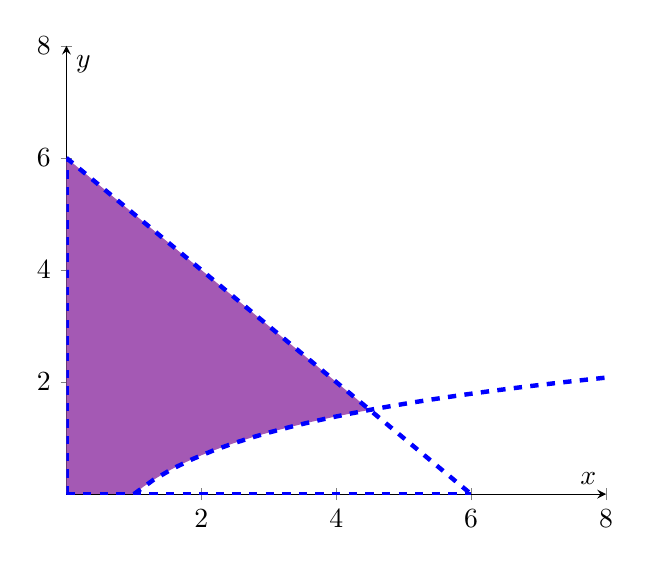
\begin{tikzpicture}[scale=1.0]
        \begin{axis}[
            axis x line=middle,
            axis y line=middle,
            ymin=0,ymax=8,ylabel=$y$,
            xmin=0,xmax=8,xlabel=$x$
        ]
            \begin{scope}
                \path[clip]
                    plot[domain=0:1] ({\x}, {0})
                    --plot[domain=1:4.49666] ({\x}, {ln(\x)})
                    --plot[domain=4.49666:0] ({\x}, {6-\x})
                    --plot[domain=0:6, variable=\y] ({0}, {\y})
                    --cycle;

                \fill [red!45!blue!65!] (0,0) rectangle (6,6);
            \end{scope}

            \plot[domain=0:6,blue,dashed,ultra thick] {6-\x};
            \plot[domain=1:8,blue,dashed,ultra thick] {ln(\x)};
            \plot[domain=0:6,blue,dashed,ultra thick] {0};
            \plot[domain=0:6,blue,dashed,ultra thick,variable=\y] ({0}, {\y});
        \end{axis}
    \end{tikzpicture}
\caption{Example feasible region (light purple) satisfying four constraints (dashed blue line)}
\label{fig:exmp-plant-feasible-region}
\end{figure}

\begin{exmp}
    Consider the problem of maximizing plant growth by manipulating quantities of two nutrients, $x_1$ and $x_2$. Let the plant height be $f(x_1, x_2) = 1 + x_1^2(x_2 - 1)^3e^{-x_1-x_2}$, with the constraints that $x_1 \geq 0$, $x_2 \geq 0$, $x_1 + x_2 \geq 6$, and $x_2 \geq \log x_1$. Then within the feasible region (depicted in Figure \ref{fig:exmp-plant-feasible-region}), $f$ is maximized by $(x_1, x_2) = (2, 4)$.
\end{exmp}

\begin{defn}
    For any $x, y \in \R^n$, the Euclidean length of $x$ is
    \[\norm{x} = \sqrt{x\cdot x} = \sqrt{\sum_{i=1}^{n}x_i^2},\]
    and the Euclidean distance between $x$ and $y$ is $\norm{x - y}$.
\end{defn}

\begin{defn}
    For all $x \in \R^n$ and $\varepsilon > 0$, the \emph{$\varepsilon$-neighborhood} of $x$ is
    \[N_{\varepsilon}(x) = \left\{y \in \R^n \compbar \norm{x - y} < \varepsilon \right\}.\]
\end{defn}

\begin{exmp}
    In $\R^1$, $N_{3}(7)$ is $(4, 10)$.
\end{exmp}

\begin{defn}
    For any $S \subseteq \R^n$ and $x \in \R^n$, we say that $x$ is an \emph{interior point} of $S$ if there exists an $\varepsilon$ neighborhood of $x$ $N_{\varepsilon}(x) \subseteq S$. If every $N_{\varepsilon}(x)$ contains a point inside $S$ and a point not inside $S$, we say that $x$ is a \emph{boundary point} of $x$.
\end{defn}

\begin{defn}
    A set $S \subseteq \R^n$ is \emph{open} if every point in $S$ is an interior point of $S$, and \emph{closed} if $S$ contains every boundary point of $S$.
\end{defn}

\begin{exmp}
    In $\R^1$, any non-empty interval $[a, b]$ is closed, and non-empty $(a, b)$ is open.
\end{exmp}

\begin{exmp}
    Both $\emptyset$ and $\R^n \subseteq \R^n$ are both open and closed.
\end{exmp}

\begin{prop}
    Let $S \subseteq \R^n$. Then $S$ is open if and only if $\R^n - S$ is closed.
\end{prop}

\begin{proof}
    Assume that $S$ is open, and let $x$ be a boundary point of $\R^n - S$. Then for every $\varepsilon > 0$, by definition there exists $y, z \in N_{\varepsilon}(x)$ such that $y \in S$ and $z \in \R^n - S$. Therefore, $N_{\varepsilon}(x) \centernot\subseteq S$. It follows that $x \notin S$ by definition, and so $x \in \R^n - S$. Therefore, $\R^n - S$ contains every boundary point of itself, and so it is closed.

    Assume that $\R^n - S$ is closed, and let $x \in S$. Consider $N_{\varepsilon}(x)$. Since $\R^n - S$ contains all of its boundary points, $x$ cannot be a boundary point of $\R^n - S$, and so we know that there must be some $\varepsilon$ such that $N_{\varepsilon} \subseteq S$. Therefore, every $x \in S$ is an interior point of $S$, and so $S$ is closed by definition.
\end{proof}

\begin{exmp}
    We will examine a few cases in which minima and maxima may fail to first.

    \begin{itemize}
        \item Unbounded objective function, e.g. minimizing $\ln x$ such that $0 < x \leq 7$.
        \item Bounded objective function on open set, e.g. minimizing $\ln x$ such that $1 < x \leq 7$.
        \item Infeasible (feasible region is empty), e.g. minimizing $\ln x$ such that $1 < x \leq 0.5$.
    \end{itemize}
\end{exmp}

\begin{exmp}
    When a solution exists, two distinct cases may occur.

    \begin{itemize}
        \item The solution is an interior point of the feasible region, e.g. minimizing $f(x) = 3 + (x - 2)^2$ such that $1 \leq x \leq 3$. The local minimum is $x^* = 2$, and $f'(x^*) = 0$.
        \item The solution is a boundary point of the feasible region, e.g. minimizing $f(x) = 3 + (x - 2)^2$ such that $x \leq 10$. Then $x^* = 10$, but $f'(x^*) \neq 0$.
    \end{itemize}
\end{exmp}

\begin{defn}
    Let $S \subseteq \R^n$ and $f: \R^n \to \R$. Consider $x^* \in S$. We say that $x^*$ is a \emph{global minimizer} if for all $y \in S$, $f(x^*) \leq f(y)$, and a \emph{strict} global minimizer if for all $y \in S - \{x^*\}$, $f(x^*) < f(y)$.
\end{defn}

\begin{defn}
    Let $S \subseteq \R^n$ and $f: \R^n \to \R$. Consider $x^* \in S$. We say that $x^*$ is a \emph{local minimizer} if there exists an $\varepsilon$-neighborhood $N_{\varepsilon}(x^*)$ such that for all $y \in N_{\varepsilon}(x) \intersection S$, $f(x^*) \leq f(y)$, and a \emph{strict} local minimizer if for all $y \in \left(N_{\varepsilon}(x) \intersection S\right) - \{x^*\}$, $f(x^*) < f(y)$.
\end{defn}

\begin{defn}
    Let $S \subseteq \R^n$ be a feasible region and $f: S \to \R$ an objective function. A \emph{stationary point} $x \in S$ is where $\nabla f(x) = \vec{0}.$
\end{defn}

\begin{rmk}
    Let $S \subseteq \R^n$, $x^*$ be an interior point of $S$, and $f: S \to \R$ be a sufficiently smooth continuous function. If $x^* \in S$ is a local minimizer, then the \emph{gradient} of $f(x^*)$ is $\vec{0}$. However, $\nabla f(x^*) = \vec{0}$ does not imply that $x^*$ is a local minimizer.
\end{rmk}

\section{Forms of Linear Programming Problems}

\begin{defn}
    A maximization or minimization linear programming problem in \emph{standard form} is a problem of the form:
    find $x \in \R^n$ that maximizes or minimizes $C \cdot x$ (also commonly seen as $C^{\transpose}x$) such that $Ax = b$ and $x \vec{0}$. The problem is said to be in \emph{canonical form} if the constraints are instead in the form $Ax \geq b$ (or $Ax \leq b$).
\end{defn}

\begin{exmp}
    Consider the problem of minimizing the cost per unit of chicken feed, while ensuring necessary nutrients are provided. Let $x_1, x_2, x_3, x_4$ denote the quantities of each of four ingredients, with cost per unit of $6.2$, $2.0$, $1.6$, and $3.2$ respectively. Let $n_1$, $n_2$, $n_3$ be the nutrients, with minimum required values of $6.2$, $11.9$, and $10.0$ respectively.

    \begin{minipage}{\linewidth}
        \begin{center}
        \captionof{table}{Nutrition values}
        \label{exmp-feed-nutrition-values}
        \begin{tabular}{c|cccc}
        & $x_1$ & $x_2$ & $x_3$ & $x_4$\\
        \hline
        $n_1$ & $1.2$ & $2.6$ & $0.0$ & $9.2$ \\ \hline
        $n_2$ & $3.9$ & $1.0$ & $0.8$ & $2.0$ \\ \hline
        $n_3$ & $6.0$ & $0.0$ & $4.0$ & $3.1$ \\
        \end{tabular}
        \end{center}
    \end{minipage}

    Let
    \[A = \begin{pmatrix}
        1.2 & 2.6 & 0.0 & 9.2 \\
        3.9 & 1.0 & 0.8 & 2.0 \\
        6.0 & 0.0 & 4.0 & 3.1
    \end{pmatrix},\; B = \begin{pmatrix}
        6.2 \\ 11.9 \\ 10.0
    \end{pmatrix},\; C = \begin{pmatrix}
        6.2 \\ 2.0 \\ 1.6 \\ 3.2
    \end{pmatrix},\; x = \begin{pmatrix}
        x_1 \\ x_2 \\ x_3 \\ x_4
    \end{pmatrix}\]
    then our problem is to minimize $C^{\transpose}x$ such that $Ax \geq b$ and $x \geq \vec{0}$. This form is the \emph{canonical form} of a linear programming problem.
\end{exmp}

\begin{rmk}
    We can easily convert problems expressed as a minimization problem into an equivalent maximization problem and vice versa, and between standard form and canonical form.
\end{rmk}

\begin{prop}
    Minimizing $C^{\transpose}x$ is equivalent to maximizing $-C^{\transpose}x$ (and so maximizing $C^{\transpose}$ is equivalent to minimizing $C^{\transpose}x$).
\end{prop}

\begin{prop}
    The constraint $Ax \geq b$ is equivalent to $-Ax \leq -b$, and $Ax \leq b$ is equivalent to $-Ax \geq -b$.
\end{prop}

\begin{prop}
    The constraint $Ax = b$ is equivalent to having both $Ax \geq b$ and $Ax \leq b$, and therefore is equivalent to $[A; -A] \geq [b; -b]$.
\end{prop}

\begin{prop}
    The constraint $Ax \geq b$ is equivalent to $Ax - z = b$, where $A \in M_{m \times n}(\R)$, $x \in \R^n$, and $z \in \R^m$ where $z \geq 0$. Here, $z$ is a vector of \emph{slack} variables.
\end{prop}

\begin{exmp}
    The constraints
    \begin{align*}
        a_{11}x_1 + a_{12}x_2 + a_{13}x_3 &\geq b_1 \\
        a_{21}x_1 + a_{22}x_2 + a_{23}x_3 &\geq b_2 \\
        a_{31}x_1 + a_{32}x_2 + a_{33}x_3 &\geq b_3 \\
        a_{41}x_1 + a_{42}x_2 + a_{43}x_3 &\geq b_4
    \end{align*}
    are equivalent to
    \begin{align*}
        a_{11}x_1 + a_{12}x_2 + a_{13}x_3 - x_4 &= b_1 \\
        a_{21}x_1 + a_{22}x_2 + a_{23}x_3 - x_5 &= b_2 \\
        a_{31}x_1 + a_{32}x_2 + a_{33}x_3 - x_6 &= b_3 \\
        a_{41}x_1 + a_{42}x_2 + a_{43}x_3 - x_7 &= b_4.
    \end{align*}
\end{exmp}

\begin{prop}
    We can incorporate the positivity constraints $x \geq 0$ into the general matrix constraints. The constraints $Ax \geq b$ and $x \geq 0$ are equivalent to \[\begin{bmatrix} A \\ I\end{bmatrix}x \geq \begin{bmatrix} b \\ 0 \end{bmatrix},\]
    and the constraints $Ax \leq b$ and $x \geq 0$ are equivalent to \[\begin{bmatrix} A \\ -I\end{bmatrix}x \leq \begin{bmatrix} b \\ 0 \end{bmatrix}.\]
\end{prop}

\begin{prop}
    We can transform an unconstrained problem into an equivalent problem with a positivity constraint.
\end{prop}

\begin{exmp}
    Consider the problem of minimizing $5x_1 + 6x_2$ such that $2x_1 - 3x_2 \geq 9$ and $x_1 + x_2 \geq -8$, with $x_1 \geq 0$ but $x_2$ unconstrained in sign. Define $x_2'$ and $x_2''$, and constrain $x_2', x_2'' \geq 0$. Let $x_2 = x_2' - x_2''$.
\end{exmp}

\begin{rmk}
    Constraints of the form $Ax = b$ are simply a system of equations, and therefore can be simplified using row operations by Theorem \ref{solutions-unchanged-by-row-ops}. Reduced row echelon form can help identified independent vs dependent variables.
\end{rmk}

\section{Polyhedrons}

\begin{defn}
    For non-zero $p \in \R^n$, the \emph{hyperplane} with normal vector $p$ is the orthogonal complement of $p$: \[\left\{x \in \R^n \compbar p \cdot x = 0 \right\},\]
    and the closed \emph{half-space} with normal vector $p$ is
    \[\left\{x \in \R^n \compbar p \cdot x \geq 0 \right\}.\]
    If we have $p \cdot x > 0$, we say it is an open half-space. We can replace $\geq$ and $>$ with $\leq$ and $<$ respectively.
\end{defn}

\begin{defn}
    A \emph{polyhedron} (or \emph{polyhedral set}) is the intersection of finitely many half spaces.
\end{defn}

\begin{defn}
    A polyhedron $P$ is \emph{bounded} if there exists $r \in \R$ such that $\norm{x} < r$ for all $x \in P$. A bounded polyhedron is known as a \emph{polytope}.
\end{defn}

\begin{prop}
    $P \subseteq \R^n$ is a polyhedron if and only if there exists $A \in M_{m \times n}(\R)$ and $b \in \R^m$ such that
    \[P = \left\{x \in \R^n \compbar Ax \geq b\right\}.\]
\end{prop}

\begin{defn}
    Let $X = \{x_1, \ldots, x_k\} \subset \R^n$. A \emph{convex combination} of $X$ is
    \[\lambda_1 x_1 + \lambda_2 x_2 + \cdots + \lambda_k x_k,\]
    where $\lambda_i \geq 0 \in \R$ and $\sum_{i=1}^{k}\lambda_i = 1$.
\end{defn}

\begin{defn}
    A set $S \subseteq \R^n$ is \emph{convex} if for any $x, y \in S$ and convex combination $z$ of $x$ and $y$, then $z \in S$.
\end{defn}

\begin{thm}
    Every polyhedron is convex.
\end{thm}

\begin{proof}
    Let $P = \left\{x \in \R^n, \compbar Ax \geq b\right\}$ be a polyhedron in $\R^n$. Let $x, y \in P$ and $z = \lambda x + (1 - \lambda) y$ be a convex combination of $x$ and $y$ for some $\lambda \in [0, 1]$.

    We know that $Ax \geq b$ and $Ay \geq b$, and want to show that $Az \geq b$. Since $z = \lambda x + (1 - \lambda)y$,
    \begin{align*}
        Az = A\left(\lambda x + (1 - \lambda)y\right) = \lambda Ax + (1 - \lambda)Ay \geq \lambda b + (1 - \lambda) b = b,
    \end{align*}
    and so $Az \geq b$.
\end{proof}

\begin{thm}
    A set $S \subseteq \R^n$ is convex if and only if every convex combination of every finite $X \in S$ is in $S$.
\end{thm}

\begin{proof}
    We will prove this by showing that this is equivalent to the definition.
    
    $(\impliedby)$ If every convex combination of finite $X \subseteq S$ is in $S$, then every convex combination of $x, y \in S$ is in $X$.

    $(\implies)$ We will prove, via induction on $n = \abs{X}$, that if $z$ is a convex combination of $x, y \in S$ implies that $z \in S$, then every convex combination of $X \in S$ is also in $S$.

    First, consider the base case of $n=1$, so $X = \{x\} \subseteq S$. The only convex combination of $X$ is simply $x$, and so every convex combination of $X$ is in $S$. Next, assume that if $z$ is a convex combination of $x, y \in S$ implies that $z \in S$, then every convex combination of $X \in S$ where $\abs{X} = n$ is also in $S$. For any $X' \in S$ where $\abs{X'} = n+1$, there is some $X \subsetneq X'$ such that $\abs{X} = n$. Then every convex combination of $X$ is in $S$. Let \[\lambda_1x_1 + \cdots + \lambda_n x_n + \lambda_{n+1}x_{n+1}\] be a convex combination of $X$. Let $\Lambda = \lambda_1 + \cdots + \lambda_n$, and note that
    \[\alpha = \frac{\lambda_1}{\Lambda}x_1 + \cdots + \frac{\lambda_n}{\Lambda}x_n\] is a convex combination of $X$ and so must be in $S$ by by the induction hypothesis. Furthermore, note that
    \[\Lambda \alpha + \lambda_{n+1}x_{n+1}\] is our original convex combination of $X'$, but is also a convex combination of two points in $S$, and so is also in $S$ by assumption.
\end{proof}

\begin{defn}
    Let $S$ be a convex set, and consider $x \in S$. If $x$ being a convex combination of $y, z \in S$ implies that $x = y = z$, we say that $x$ is an \emph{extreme point}.
\end{defn}

\section{Basic Feasible Solutions}

\begin{defn}
    Let $c \in \R^n$, $A \in M_{m \times n}(\R)$, and $b \in \R^m$ be the linear program with feasibility region \[S = \left\{x \in \R^n \compbar Ax = b, x \geq \vec{0}\right\}.\] Let $A$ have rank $m$, or else eliminate redundant constraints until it does.

    Let $B$ be a subset of $m$ of the indices $\{1, \ldots, n\}$ such that the corresponding columns of $A$ form a basis for the column space of $A$ (which is $\R^m$ since $A$ has rank $m$). Let $A_B \in M_{m \times m}(\R)$ denote the invertible matrix of these columns.

    A \emph{basic feasible solution} is any $x \in S$ where $j \notin B$ implies $x_j = 0$.
\end{defn}

\begin{rmk}
    Without loss of generality, we can rearrange the columns of $A$ such that $A = [A_B | N]$, and then basic feasible solutions are precisely those $x \in S$ such that $x = \begin{bmatrix}
        x_B \\ x_N
    \end{bmatrix}$ where $x_N = \vec{0}$.
\end{rmk}

\begin{thm}
    Let $B \in M_{m \times m}(\R)$ have rank $m$, and $N \in M_{m \times (n-m)}(\R)$ where $m < n$, and then let $A = [B | N] \in M_{m \times n}(\R)$. Let $b \in \R^m$, so the feasible region is \[S = \left\{x \in \R^n \compbar Ax = b,\; x \geq \vec{0}\right\}.\]

    Then $x \in S$ is an extreme point of $S$ if and only if $x$ is a basic feasible solution of $S$.
\end{thm}

\begin{proof}\proofbreak
    ($\impliedby$) Suppose $x$ is a basic feasible solution of $S$, so $x = \begin{bmatrix}
        x_B \\ x_N
    \end{bmatrix}$ where $x_N = \vec{0}$. Let $x = \lambda x' + (1 - \lambda) x''$ be a non-trivial convex combination (so $0 < \lambda < 1$) of $x', x'' \in S$. We can write $x', x''$ as $x' = \begin{bmatrix} x_B'' \\ x_N'' \end{bmatrix}$ and $x'' = \begin{bmatrix} x_B'' \\ x_N'' \end{bmatrix}$. Notice that we now have $x_N = \vec{0} = \lambda x_N' + (1 - \lambda)x_N''$. Since $x', x'' \in S$, we know $x_N', x_N'' \geq 0$ and so we necessarily have $x_N' = x_N'' = 0$. But then $x'$ and $x''$ are also basic feasible solutions. Since $B$ is invertible and $x, x', x'' \in S$, we know that $Bx_B = Bx_B'b = Bx_B''$, and so $x = x' = x''$.

    ($\implies$) Suppose $x$ is not a basic feasible solution of $S$. Then $x = \begin{bmatrix}
        x_B \\ x_N
    \end{bmatrix}$ where $x_N$ is nonzero. We know that the columns of $A$ corresponding to the non-zero entries of $x$ must be linearly dependent, or else we can complete them to a basis for $\R^m$ and $x$ would be a basic feasible solution. Therefore, we know there exists $z$ such that $Az = \vec{0}$ and $z_i \neq 0$ implies $x_i \neq 0$. Note that for any $\alpha \in \R$, $A(x + \alpha z) = Ax + \alpha Az = b$, so any $x + \alpha z \geq \vec{0}$ is a feasible solution. Since $x_i$ is strictly greater than zero when $z_i \neq 0$, for sufficiently small $\varepsilon$ the points $x + \varepsilon z$ and $x - \varepsilon z$ must be feasible. Then $x = \frac{1}{2}\left(x + \varepsilon z\right) + \left(1 - \frac{1}{2}\right)\left(x - \varepsilon z\right)$, and so $x$ can be expressed as a non-trivial convex combination in $S$ and therefore is not extreme.
\end{proof}

\section{Simplex Method}

\begin{defn}
    Consider a linear program in standard form. Given a choice of basis $B$ such that $A = [B | N]$, the \emph{pre-tableau} is the matrix
    \begin{align*}
        \left[\begin{array}{c|c|c|c}
            1 & -c_B^{\transpose} & -c_N^{\transpose} & 0 \\
            \hline
            \vec{0} & B & N & b
        \end{array}\right].
    \end{align*}
    In other words, we have augment $A = [B|N]$ with the constraint values $b$, and then again with a new variable $z$ in the first column/row such that $z - c^{\transpose}x = 0$. Note that $z$ is therefore the value of the objective function.
\end{defn}

\begin{defn}
    Given a linear program in standard form, and basic feasible solution $x^{\transpose} = [x_B^{\transpose}, \vec{0}]$, the corresponding \emph{basic feasible simplex tableau} is the matrix
    \begin{align*}
        \left[\begin{array}{c|c|c|c}
            1 & 0 & c_B^{\transpose}B^{-1}N-c_N^{\transpose} & c_B^{\transpose}B^{-1}b \\
            \hline
            \vec{0} & I & B^{-1}N & B^{-1}b
        \end{array}\right].
    \end{align*}
\end{defn}

\begin{rmk}
    The basic feasible tableau is the reduced row echelon form of the pre-tableau. It can also be obtain by left-multiplying the pre-tableau by
    \begin{align*}
        \left[\begin{array}{c|c}
            1 & c_B^{\transpose}B^{-1} \\
            \hline
            \vec{0}^{\transpose} & B^{-1}
        \end{array}\right].
    \end{align*}
\end{rmk}

\begin{rmk}
    We can see that $z + (c_B^{\transpose}B^{-1}N-c_N^{\transpose})x_N = c_B^{\transpose}B^{-1}b$, so $z = c_B^{\transpose}B^{-1}b + (c_N^{\transpose} - c_B^{\transpose}B^{-1}N)x_N$. We often denote this as
    \[z = c_B^{\transpose}B^{-1}b + r_N^{\transpose}x_N,\]
    where
    \[r_N^{\transpose} = c_N^{\transpose} - c_B^{\transpose}B^{-1}N.\]
\end{rmk}

In the simplex, we start with a linear program $A, b, c$ in standard form. Assuming we already know a basis that leads to a basic feasible solution, we form the pre-tableau and either row-reduce or multiply through by the matrix from the above remark to obtain the basis feasible tableau.

To illustrate the linear program, we will consider
\begin{align*}
    A =
    \begin{bmatrix}
        2 & -1 & 3 & 7 & 1 & 2 & 8 \\
        5 & 2 & -8 & -1 & 2 & 0 & 1 \\
        4 & 6 & -2 & 4 & 1 & 3 & -5
    \end{bmatrix},\;\;
    b = \begin{bmatrix}
        2 \\ 4 \\ 3
    \end{bmatrix},\;\;
    c^{\transpose} = [6, -3, 2, 1, -1, 7, 1].
\end{align*}

We will use columns $1$, $3$, and $7$ as our basis columns, however we will leave the columns in their original order to make bookkeeping easier. Our pre-tableau is
\begin{align*}
    \left[\begin{array}{c|ccccccc|c}
        1 & -6 & 3 & -2 & -1 & 1 & -7 & -1 & 0 \\
        \hline
        0 & 2 & -1 & 3 & 7 & 1 & 2 & 8 & 2 \\
        0 & 5 & 2 & -8 & -1 & 2 & 0 & 1 & 4 \\
        0 & 4 & 6 & -2 & 4 & 1 & 3 & -5 & 3
    \end{array}\right].
\end{align*}

Row-reducing to the reduced row echelon form (while treating columns $1$, $3$, and $7$ as leading columns) brings us to our first basic feasible tableau:
\begin{align*}
    \left[\begin{array}{c|ccccccc|c}
        1 & 0 & 9.35 & 0 & 11.06 & 2.82 & -1.22 & 0 & 4.93 \\
        \hline
        0 & 1 & 1.03 & 0 & 1.62 & 0.31 & 0.82 & 0 & 0.81 \\
        0 & 0 & 0.33 & 1 & 1.14 & -0.05 & 0.50 & 0 & 0.01 \\
        0 & 0 & -0.51 & 0 & 0.04 & 0.07 & -0.14 & 1 & 0.04
    \end{array}\right].
\end{align*}

Now, we \emph{pivot} to a new (and improved!) basic feasible tableau by choosing a non-basis column to turn into a basis column. We make the greediest choice by choose the $4$th column ($5$th of the overall tableau) since it has the largest improvements to our objective function per unit chance in the corresponding non-basis variable.

Letting $j = 4$, we choose the $k$th row (excluding the objective row on top) by \[\argmin_{k}\frac{b_k}{A_{kj}} \mathrm{ where } A_{kj} \geq 0.\] This gives us the $2$nd row, so we row-reduce again, replace the column whose leading term choose in the $2$nd row (which is column $3$) with column $4$. To do this, we treat column $4$ as if it was the second column while row-reducing. Our new basis columns are $1$, $4$, and $7$, giving us our second basic feasible tableau:
\begin{align*}
    \left[\begin{array}{c|ccccccc|c}
        1 & 0 & 6.14  & -9.67 & 0 & 3.29  & -6.01 & 0 & 4.81 \\
        \hline
        0 & 1 & 0.56  & -1.41 & 0 & 0.37  & 0.11  & 0 & 0.79 \\
        0 & 0 & 0.28  & 0.87  & 1 & -0.04 & 0.43  & 0 & 0.01 \\
        0 & 0 & -0.57 & -0.03 & 0 & 0.06  & -0.15 & 1 & 0.04
    \end{array}\right].
\end{align*}

Note that the objective function value has decreased from $4.93$ to $4.81$. We now continue pivoting in the manner, the objective function value decreasing from $4.81$, to $4.6$, to $-2.45$, to $-2.46$. When there are no positive entries in the objective function row (top row), there are no more improvements that can be made by changing our choice of basis and we have reached optimality.

\subsection{Two-Phase Method}

The Two-Phase Method is a technique for coming up with the initial basic feasible solution need to start off the Simplex Method. In Phase I, we solve a different linear program to find the initial basic feasible solution, and then in Phase II we use that basic feasible solution to apply the simplex method to the original linear program. We take a problem in standard form with constraints $Ax = b$, $x \geq 0$ where $A \in M_{m \times n}(\R)$. We then introduce \emph{artificial variables} $x_{n+1}, x_{n+2}, \ldots, x_{n+m}$ for each constraint (row) in $A$. Let $x'$ denote the vector obtained by appending the artificial variables to $x$.

For Phase I, we solve a different problem using the Simplex Method: minimizing $x_{n+1} + x_{n+2} + \cdots + x_{n+m}$ such that $[A|I]x' = b$, $x' \geq 0$. Notice that any feasible solution to this new problem is a feasible solution to the original linear program if the objective function value is zero. Therefore, the $x$ part of an optimal solution $x'$ to the new problem is a feasible solution to the original if $x'$ has objective function value zero. If the optimal solution $x'$ has a positive objective function value, then no feasible solution exists for the original linear program.

Note that
\begin{align*}
    x' = \begin{bmatrix}
        x \\
        x_{n+1} \\
        \vdots \\
        v_{n+m}
    \end{bmatrix} = \begin{bmatrix}
        0 \\
        b_1 \\
        \vdots \\
        b_m
    \end{bmatrix}
\end{align*}
is always a basic feasible solution to the Phase I problem. Therefore, we can immediately apply the Simplex method to determine the feasibility of the original linear program, and find a feasible solution if one exists. Additionally, since the number of columns in a basis for either linear program is the same (always just $m$), the feasible solution given to us by Phase I must in fact be a basic feasible solution for Phase II.

\subsection{Big-M Method}

In the Big-M method, we do essentially the same process, but in one phase instead of two. We do this by using an objective function of
\begin{align*}
    c^{\transpose}x + M(x_{n+1} + x_{n+2} + \cdots + x_{n+m}),
\end{align*}
where $M$ is a very large value. This penalizes the artificial variables and causes them to be zero in any optimal solution. Setting the artificial variables to $b$ gives us an initial basic feasible solution. If a basic feasible solution exists where the artificial variables are zero, the first $m$ pivots will replace each artificial variable with non-artificial variables, and so the final optimal solution will be a solution to the original linear program.

\section{Duality}

\begin{defn}{Canonical or symmetric duality}\proofbreak
    Consider a linear program of the form minimize $c^{\transpose}x$ such that $Ax \geq b$ and $x \geq \vec{0}$. The \emph{dual} problem is maximizing $b^{\transpose}y$ such that $A^{\transpose}y \leq c$ and $y \geq \vec{0}$. The original linear program is referred to as the \emph{primal} probem in relation to its dual.
\end{defn}

\begin{exmp}
    Consider minimizing $1x_1 + 2x_2$ such that
    \begin{align*}
        3x_1 + 4x_2 &\geq 9, \\
        5x_1 + 6x_2 &\geq 10, \\
        7x_1 + 8x_2 &\geq 11, \\
        x_1, x_2 &\geq 0.
    \end{align*}

    The dual problem is maximizing $9y_1 + 10y_2 + 11y_3$ such that
    \begin{align*}
        3y_1 + 5y_2 + 7y_3  &\leq 1, \\
        4y_1 + 6y_2 + 8y_3  &\leq 2, \\
        y_1, y_2, y_3 &\geq 0.
    \end{align*}
\end{exmp}

\begin{defn}{Standard duality}\proofbreak
    Consider a linear program of the form minimization of $c^{\transpose}x$ such that $Ax = b$ and $x \geq \vec{0}$. The \emph{dual} problem is maximizing $b^{\transpose}y$ such that $A^{\transpose}y \leq c$, \emph{without} a non-negativity constraint on $y$. The original linear program is again referred to as the \emph{primal} probem in relation to its dual.
\end{defn}

\begin{rmk}
    We can derive the canonical form of duality from the standard form, and vice versa. Imagine we know that the dual of minimizing $c^{\transpose}x$ such that $Ax = b$ and $x \geq \vec{0}$ was to maximize $b^{\transpose}y$ such that $A^{\transpose}y \leq c$. If we were now given a linear program in canonical form and wanted to find its dual, we could first convert it into standard form by the introduction of slack variables, obtaining minimize $c^{\transpose}x$ such that $[A|-I]\begin{bmatrix}x \\ z\end{bmatrix} = b$ such that $\begin{bmatrix}x \\ z\end{bmatrix} \geq 0$. The standard dual of this is to maximize $b^{\transpose}y$ such that $[A|-I]^{\transpose}y \leq \begin{bmatrix}c \\ \vec{0}\end{bmatrix}$, which is equivalent to maximizing $b^{\transpose}y$ such that $A^{\transpose}y \leq c$ and $y \geq \vec{0}$ (from $-y \leq \vec{0}$).
\end{rmk}

\begin{prop}
    The canonical and standard duals of equivalent linear programs are equivalent.
\end{prop}

\begin{proof}\proofbreak
    \begin{figure}[ht]
        \centering
        \begin{tikzpicture}[{baseline=(current bounding box.north)}]
            \node[align=center] at (-3,2.5) {$
                \begin{aligned}
                    \mathrm{min.}\;c^{\transpose}&x \\
                    \mathrm{s.t.}\;A&x \geq b, \\
                          &x \geq \vec{0}.
                \end{aligned}
            $};
            \node[align=center] at (3,2.5) {$
                \begin{aligned}
                    \mathrm{max.}\;b^{\transpose}&y \\
                    \mathrm{s.t.}\;A^{\transpose}&y \leq c, \\
                          &x \geq \vec{0}.
                \end{aligned}
            $};
            \node[align=center] at (-3,-3) {$
                \begin{aligned}
                    \mathrm{min.}\;\begin{bmatrix}c \\ \vec{0}\end{bmatrix}^{\transpose}&\begin{bmatrix}x \\ z\end{bmatrix} \\
                    \mathrm{s.t.}\;\left[A|-I\right]&\begin{bmatrix}x \\ z\end{bmatrix} = b, \\
                          &x, z \geq \vec{0}.
                \end{aligned}
            $};
            \node[align=center] at (3,-3) {$
                \begin{aligned}
                    \mathrm{max.}\;&b^{\transpose}y \\
                    \mathrm{s.t.}\;&\begin{bmatrix}A^{\transpose} \\ -I\end{bmatrix}y \leq \begin{bmatrix}c \\ \vec{0}\end{bmatrix}.
                \end{aligned}
            $};

            \draw[ultra thick, blue, ->] (-1, 3) -- (1, 3);
            \draw[ultra thick, red, ->] (-1, -3) -- (1, -3);
            \draw[ultra thick, black, <->] (3, -1) -- (3, 1);
            \draw[ultra thick, black, <->] (-3, 1) -- (-3, -1);

        \end{tikzpicture}
    \end{figure}
\end{proof}

\begin{prop}
    Given a primal linear program, the dual of the dual is the primal.
\end{prop} 

\begin{proof}
    Consider a linear program in canonical form.  By definition, the dual is maximizing $b^{\transpose}y$ such that $A^{\transpose}y \leq c$ and $y \geq 0$. This program is equivalent to minimizing $-b^{\transpose}y$ such that $-A^{\transpose}y \geq -c$ and $y \geq 0$. The dual of this equivalent form of the dual is to maximizing $-c^{\transpose}x$ such that $\left(-A^{\transpose}\right)^{\transpose}x \leq -b$ and $x \geq 0$. Finally, this program is equivalent to minimizing $c^{\transpose}x$ such that $Ax \geq b$ and $x \geq 0$, which is the primal linear program.
\end{proof}

\begin{thm}{Weak Duality}\label{weak-duality}\proofbreak
    Consider a linear program and its dual, and $x, y$ feasible solutions to the primal and dual programs respectively. Then the objective function value at $y$ in the dual is less than or equal to the objective function value at $x$ in the primal.
\end{thm}

\begin{proof}
    When the primal is in standard form, we have $Ax = b$, $x \geq \vec{0}$ and $A^{\transpose}y \leq c$. It follows that $b^{\transpose}y = (Ax)^{\transpose}y = x^{\transpose}A^{\transpose}y$. Since we have $x \geq \vec{0}$, we know that $x^{\transpose}A^{\transpose}y \leq x^{\transpose}c$, and so $b^{\transpose}y \leq c^{\transpose}x$.

    When the primal is in canonical form, we have $Ax \geq b$, $x \geq \vec{0}$, $A^{\transpose}y \leq c$, and $y \geq 0$. Since $y \geq \vec{0}$, $Ax \geq b$ implies that $b^{\transpose}y \leq (Ax)^{\transpose}y$, and so $b^{\transpose}y \leq x^{\transpose}A^{\transpose}y$. Furthermore, since $A^{\transpose}y \leq c$ and $x \geq \vec{0}$, $x^{\transpose}A^{\transpose}y \leq x^{\transpose}c = c^{\transpose}x$. Combining these, we arrive at $b^{\transpose}y \leq c^{\transpose}y$.
\end{proof}

\begin{cor}
    The optimal objective value function in the dual is less than or equal to the optimal objective function value in the primal.
\end{cor}

\begin{cor}{Supervisor principle}\label{supervisor-principle}\proofbreak
    If $b^{\transpose}y = c^{\transpose}x$, then $x$ and $y$ are optimal in their respective linear programs.
\end{cor}

\begin{thm}{Strong Duality}\label{strong-duality}\proofbreak
    Suppose a linear program has a feasible solution and its objective function is unbounded. Then the linear program and its dual have optimal solutions $x$ and $y$ respectively, and the objective function value of $x$ and $y$ are equal.
\end{thm}

\begin{proof}
    Consider the primal in standard form. We can apply the Simplex method or similar to obtain an optimal basic feasible solution $x^*$. Without loss of generality, we can assume that the final basis consists of the first $m$ columns of $A$.

    By the terminating condition of the Simplex method, we know that
    \begin{align*}
        r_N^{\transpose} = c_N^{\transpose} - c_B^{\transpose}B^{-1}N \geq \vec{0}.
    \end{align*}
    Let
    \begin{align*}
        {y^*}^{\transpose} = c_B^{\transpose}B^{-1}.
    \end{align*}

    Since $r_N^{\transpose} \geq \vec{0}$, we know that
    \begin{align*}
        c_B^{\transpose}B^{-1}N \leq c_N^{\transpose},
    \end{align*}
    and so it follows that
    \begin{align*}
        {y^*}^{\transpose}A = c_B^{\transpose}B^{-1}[B|N] = [c_B^{\transpose}|c_B^{\transpose}B^{-1}N] \leq [c_B^{\transpose}|c_N^{\transpose}] = c^{\transpose},
    \end{align*}
    so $y^*$ is a feasible solution to the dual. Now we can show that the objective function values are equal:
    \begin{align*}
        {y^{*}}^{\transpose}b = c_B^{\transpose}B^{-1}b = \begin{bmatrix}c_B \\ \vec{0}\end{bmatrix}^{\transpose}\begin{bmatrix}x_B \\ \vec{0}\end{bmatrix} = c^{\transpose}x^*.
    \end{align*}

    Therefore, $y^*$ is an optimal solution to the dual linear program by the supervisor principle \ref{supervisor-principle}.
\end{proof}

\section{Sensitivity Analysis}

\begin{defn}
    A basic feasible solution $b$ to a linear program with basis $B$ is \emph{non-degenerate} when $B^{-1}b > \vec{0}$.
\end{defn}

Consider solving a linear program $A, b, c$ in standard form by the Simplex method. What happens if we replace $b$ with $b' = b + \Delta b$ for some arbitrary $\Delta b$? If we replaced $B^{-1}b$ with $B^{-1}(b + \Delta b)$ and $c_B^{\transpose}B^{-1}b$ with $c_B^{\transpose}B^{-1}(b + \Delta b)$ in just the final basic feasible simplex tableau, what happens?

If $B^{-1}(b + \Delta b) \geq \vec{0}$, then we still have a basic feasible solution! Furthermore, since the objective row would still be non-positive, our solution would also be an \emph{optimal} basic feasible solution. This would very likely only occur when $\Delta b$ is fairly small.

If the linear program is non-degenerate, there always exists such $\Delta b$ small enough.

In the corresponding dual linear program, we know that
\begin{align*}
    {y^*}^{\transpose} = c_B^{\transpose}B^{-1}.
\end{align*}
We also have $c^{\transpose}x^* = {y^*}^{\transpose}b$, and so when we replace $b$ with $b'$ we get
$c^{\transpose}{x'}^{*} = {y^*}^{\transpose}(b + \Delta b) = {y^*}^{\transpose}b + {y^*}^{\transpose}\Delta b$. Therefore,
\begin{align*}
    \frac{c^{\transpose}x}{\partial b_i} = y_i^*.
\end{align*}

\begin{defn}
    Vectors $x, y \in \R^n$ are \emph{complementary} if $x_i \neq 0 \implies y_i = 0$ and $y_i \neq 0 \implies x_i = 0$.
\end{defn}

\begin{prop}\label{complementary-orthogonal}
    If $x \geq 0$ and $y \geq 0$, then $x$ and $y$ are complementary if and only if $x^{\transpose}y = 0$.
\end{prop}

\begin{proof}
    If $x$ and $y$ are complementary, then $x_iy_i = 0$, and so $x^{\transpose}y = 0$.

    Since $x \geq 0$ and $y \geq 0$, we know $x_iy_i \geq 0$. If $x^{\transpose}y = 0$, then we must have $x_iy_i = 0$. Therefore at least one of $x_i$ and $y_i$ is zero and so $x$ and $y$ are complementary.
\end{proof}

\begin{thm}{Complementary slackness}\label{complementary-slackness}\proofbreak
    Consider a linear program $A, b, c$ in standard form. Let $x \in \R^n$ be a feasible solution. Let $y \in \R^m$ be a feasible solution in the dual. Then $x$ and $y$ are optimal solutions if and only if $c - A^{\transpose}y$ is complentary to $x$.
\end{thm}

\begin{proof}
    Recall that
    \begin{align*}
        b^{\transpose}y = (Ax)^{\transpose}y = x^{\transpose}A^{\transpose}y \leq x^{\transpose}c = c^{\transpose}x.
    \end{align*}
    By the supervisor principle \ref{supervisor-principle}, $x$ and $y$ are optimal if and only if $b^{\transpose}y = c^{\transpose}x$, which is equivalent to $x^{\transpose}A^{\transpose}y = x^{\transpose}c$. Therefore,
    \begin{align*}
        x^{\transpose}\left(c - A^{\transpose}y\right) = \vec{0}.
    \end{align*}

    Since $y$ is feasible in the dual, by definition $A^{\transpose}y \leq c$, and so $c - A^{\transpose}y \geq \vec{0}$. Furthermore, $x \geq 0$ and so by Proposition \ref{complementary-orthogonal} it follows that this occurs precisely when $x$ and $c - A^{\transpose}y$ are complementary.
\end{proof}

\chapter{Probability}
\label{ch:probability}

\section{Axioms of Probability}

\begin{defn}\proofbreak
    \begin{itemize}
        \item Sample point: a possible outcome of a probabilistic experiment, often denoted by $\omega$.
        \item Sample space: the set of all sample points, often denoted by $\Omega$.
        \item Event: any subset of the sample space.
    \end{itemize}
\end{defn}

\begin{defn}
    If events $A_i \subseteq \Omega$ are disjoint, we say that these events are \emph{mutually exclusive}.
\end{defn}

\begin{defn}\label{kolmogorov-probability-axioms}
    A \emph{probability space} is a sample space $\Omega$ together with a function $P: \mathcal{P}(\Omega) \to \R$ that satisfies the following axioms:
    \begin{itemize}
        \item Non-negativity: for any event $A \subseteq \Omega$, $P(A) \geq 0$.
        \item Normalization: $P(\Omega) = 1$.
        \item Countable-additivity: if $A_i$ are a countable sequence of mutually exclusive events, then $P(\disjointunionbig_{i}A_i) = \sum_{i}P(A_i)$.
    \end{itemize}
\end{defn}

\begin{rmk}
    These axioms are due to Andrey Kolmogorov.
\end{rmk}

\begin{prop}
    Let $(\Omega, P)$ be a probability space, and $A \subseteq \Omega$ an event. Then $P(A) + P(A^{c}) = 1$.
\end{prop}

\begin{proof}
    Since $A$ and $A^{c}$ are mutually exclusive, $P(A) + P(A^{c}) = P(A \union A^{c}) = P(\Omega) = 1$.
\end{proof}

\begin{cor}
    $P(\emptyset) = 0$.
\end{cor}

\begin{prop}Monotonicity\label{probability-monotonicity}\proofbreak
    Let $A, B \subseteq \Omega$ be events such that $A \subseteq B$. Then $P(A) \leq P(B)$.
\end{prop}

\begin{proof}
    Let $C = B - A$. Then $A \union C = B$ and $A \intersection C = \emptyset$. Since $A$ and $C$ are therefore mutually exclusive, $P(A) + P(C) = P(A \union C) = P(B)$. Since $P(C) \geq 0$ by the axiom of non-negativity, it follows that $P(A) \leq P(B)$.
\end{proof}

\begin{thm}{Inclusion-exclusion Principle}\label{inclusion-exclusion}
    Let $A, B, C \subseteq \Omega$ be events. Then
    \[P(A \union B) = P(A) + P(B) - P(A \intersection B),\]
    and
    \begin{align*}
        P(A \union B \union C) &= P(A) + P(B) + P(C) \\
                               &- P(A \intersection B) - P((A \intersection C) - P(B \intersection C) \\
                               &+ P(A \intersection B \intersection C).
    \end{align*}
\end{thm}

\begin{proof}
    Since $A \union B = (A - B) \union (B - A) \union (A \intersection B)$, which are necessarily mutually exclusive events, we have
    \[P(A \union B) = P(A - B) + P(B - A) + P(A \intersection B).\]
    Now note that $A = (A - B) \union (A \intersection B)$ and $B = (B - A) \union (A \intersection B)$, and so $P(A) = P(A - B) + P(A \intersection B)$ and $P(B) = P(B - A) + P(A \intersection B)$. Therefore, \begin{align*}
        P(A \union B) &= P(A - B) + P(B - A) + P(A \intersection B) \\
                      &= \big[P(A - B) + P(A \intersection B)\big] + \big[P(B - A) + P(A \intersection B)\big] - P(A \intersection B) \\
                      &= P(A) + P(B) - P(A \intersection B).
    \end{align*}

    To prove the three-way version of the principle, we can apply the two-way version to $A \union B$ and $C$. This gives us
    \begin{align*}\label{inclusion-exclusion-three-intermediate}\tag{$1$}
        P(A \union B \union C) &= P(A \union B) + P(C) - P((A \union B) \intersection C) \\
        &= \big[P(A) + P(B) - P(A \intersection B)\big] + P(C) - P((A \union B) \intersection C).
    \end{align*}
    Since $(A \union B) \intersection C = (A \intersection C) \union (B \intersection C)$, we can apply the principle again to find that
    \[P((A \union B) \intersection C) = P(A \intersection C) + P(B \intersection C) - P((A \intersection C) \intersection (B \intersection C)).\] Noting that $(A \intersection C) \intersection (B \intersection C) = A \intersection B \intersection C$ and substituting this back into \ref{inclusion-exclusion-three-intermediate}, we obtain
    \begin{align*}
        P(A \union B \union C) &= P(A) + P(B) + P(C) - P(A \intersection B) - \big[P(A \intersection C) + P(B \intersection C) - P(A \intersection B \intersection )\big] \\
        &= P(A) + P(B) + P(C) \\
        &- P(A \intersection B) - P((A \intersection C) - P(B \intersection C) \\
        &+ P(A \intersection B \intersection C).
    \end{align*}
\end{proof}

\begin{prop}
    \[A \union B = A \disjointunion (B - A).\]
    \[A \union B \union C = A \disjointunion (B - A) \disjointunion (C - (A \union B)).\]
\end{prop}

\begin{exmp}{Finite, equally-likely probability law}\proofbreak
    Let $(\Omega, P)$ be a sample space together with a function $P: \mathcal{P}(\Omega) \to \R$, where $\abs{\Omega} \in \Z^{+}$ and for all $A \in \mathcal{\Omega}$, \[P(A) = \frac{\abs{A}}{\abs{\Omega}}.\]

    Since $\abs{A} \geq 0$ and $\abs{\Omega} > 0$, $P(A) \geq 0$ and so this model satifies the non-negativity axiom. Since $P(\Omega) = \frac{\abs{\Omega}}{\abs{\Omega}} = 1$, this model satisfies the normalization axiom.
    
    Let $A = A_1 \disjointunion A_2 \disjointunion \cdots$. Then
    \begin{align*}
        P(A) = \frac{\abs{A_1 \disjointunion A_2 \disjointunion \cdots}}{\abs{\Omega}} = \frac{\abs{A_1}}{\abs{\Omega}} + \frac{\abs{A_2}}{\abs{\Omega}} + \cdots = P(A_1) + P(A_2) + \cdots,
    \end{align*}
    and so this model also satisfies the countable-additivity axiom. Therefore, it is a probability space.
\end{exmp}

\begin{exmp}{Discrete probability law}\proofbreak
    Let $\Omega$ be a sample space such that $\abs{\Omega}$ is countable, and let $M: \Omega \to R$ be a mass-function: $M(\omega) \geq 0$ for all $\omega \in \Omega$, and $\sum_{\omega \in \Omega}M(\omega) = 1$.

    Now consider $P: \mathcal{P}(\Omega) \to \R$ defined by
    \[P(A) = \sum_{\omega \in A}M(\omega).\]

    Since $M(\omega) \geq 0$, $P(A) \geq$ and so $P$ satisfies the axiom of non-negativity. Since \[P(\Omega) = \sum_{\omega \in \Omega}M(\omega) = 1\] by the definition of $M$, $P$ satisfies the axiom of normalization. Finally, for $A = A_1 \disjointunion A_2 \disjointunion \cdots$,
    \begin{align*}
        P(\disjointunionbig_{i}A_i) = \sum_{i}P(A_i) = \sum_{i}\sum_{\omega \in A_i}M(\omega) = \sum_{\omega \in A}M(\Omega) = P(A).
    \end{align*}
    Therefore, $P$ satisfies the axiom of countable additivity and so $(\Omega, P)$ is a probability space.
\end{exmp}


\begin{exmp}{Geometric probability law}\proofbreak
    Let $\Omega = \{\omega_1, \omega_2, \ldots\}$ be a sample space such that $\abs{\Omega} = \abs{\Z}$, and define $P: \mathcal{P}(\Omega) \to \R$ by
    \[P(A) = \sum_{\omega_i \in A}\left(\frac{1}{2}\right)^{i}.\]
    
    Since $\left(\frac{1}{2}\right)^i \geq 0$, $P(A) \geq 0$ and so $P$ satisfies the axiom of non-negativity. Since
    \begin{align*}
        P(\Omega) = \sum_{\omega_i \in \Omega}\left(\frac{1}{2}\right)^{i} = \sum_{i=1}^{\infty}\left(\frac{1}{2}\right)^{i} = \frac{1/2}{1 - 1/2} = 1,
    \end{align*}
    we know that $P$ satisfies the axiom of normalization.

    Finally, for $A = A_1 \disjointunion A_2 \disjointunion \cdots$,
    \begin{align*}
        P(\disjointunionbig_{i}A_i) = \sum_{\omega_j \in A}\left(\frac{1}{2}\right)^{j} = \sum_{i}\sum_{\omega_j \in A_i}\left(\frac{1}{2}\right)^{j} = \sum_{i}P(A_i).
    \end{align*}
    Therefore, $P$ satisfies the axiom of countable additivity and so $(\Omega, P)$ is a probability space.
\end{exmp}

\section{Conditional Probability}

\begin{exmp}
    Roll two six-sided dice, and only look at one of them. It is a six. Let $S$ denote the event that the sum of the values of the two dice is seven, and $A$ is the event that at least one of dice was a six. What is the probability of $P(S | A)?$ It is $\frac{2}{11}$, not $\frac{1}{6}$.
\end{exmp}

\begin{defn}
    Let $A, B \in \Omega$. Then the probability that $A$ occurred, given that $B$ occured, is denoted by $P(A | B)$ and read as ``the probability of $A$ given $B$''.
\end{defn}

\begin{prop}
    If all sample points in $\Omega$ are equally likely, then $P(A | B) = \frac{P(A \intersection B)}{P(B)}$.
\end{prop}

\begin{cor}
    $P(A \intersection B) = P(A | B)P(B)$.
\end{cor}

\begin{thm}
    Let $(\Omega, P)$ be a probability space, and $B \subseteq \Omega$ an event such that $P(B) > 0$. Then $(B, P(\cdot | B))$ form a probability space.
\end{thm}

\begin{proof}
    To show that $(B, P(\cdot|B))$ is a probability space, we need to show non-negativity (that $P(A | B) \geq 0$ for all $A$), normalization (that $P(B|B) = 1$), and countable additivity (that $P(A_1 \disjointunion A_2 \disjointunion \cdots | B) = P(A_1 | B) + P(A_2 | B) + \cdots$ if $A_i$ is a countable sequence).

    For any $A \subseteq B$, we know that $P(A \intersection B), P(B) \geq 0$, and so \[P(A | B) = \frac{P(A \intersection B)}{P(B)} \geq 0.\]

    \[P(B | B) = \frac{P(B \intersection B)}{P(B)} = \frac{P(B)}{P(B)} = 1.\]

    \begin{align*}
        P(A_1 \disjointunion A_2 \disjointunion \cdots | B) &= \frac{P\left((A_1 \disjointunion A_2 \disjointunion \cdots) \intersection B\right)}{P(B)} = \frac{P(A_1 \intersection B) \disjointunion (A_2 \intersection B) \disjointunion \cdots)}{P(B)} \\
        &= \frac{P(A_1 \intersection B) + P(A_2 \intersection B) + \cdots)}{P(B)} = \frac{P(A_1 \intersection B)}{P(B)} + \frac{P(A_2 \intersection B)}{P(B)} + \cdots \\
        &= P(A_1 | B) + P(A_2 | B) + \cdots.
    \end{align*}
\end{proof}

\begin{exmp}
    Consider a sequence of coin tosses. Let $B$ be the event that the first head of the sequence occurs on an odd numbered toss (the first toss is \#1), and let $A$ be the event that the event first coin toss lands on heads. What is $P(A | B)$?

    Since $A \subseteq B$, we know that $A \intersection B = A$. Furthermore, $P(A) = \frac{1}{2}$, and $P(B) = \frac{1}{2} + \frac{1}{8} + \cdots = \frac{1/2}{1-1/4} = \frac{1}{2}\cdot\frac{4}{3} = \frac{2}{3}$. Therefore, \[P(A | B) = \frac{P(A \intersection B)}{P(B)} = \frac{P(A)}{P(B)} = \frac{1}{2}\cdot\frac{3}{2} = \frac{3}{4}.\]
\end{exmp}

\begin{thm}Law of Total Probability\label{total-probability}\proofbreak
    Let $B_1, \ldots, B_n \in \Omega$ be mutually exclusive and exhaustive events. Then for any event $A \in \Omega$,
    \[P(A) = \sum_{i=1}^{n}P(A \intersection B_i) = \sum_{i=1}^{n}P(A | B_i)P(B_i).\]
\end{thm}

\begin{proof}
    Note that if $x \in (A \intersection B_i)$ and $x \in (A \intersection B_j)$, then $x \in B_i$ and $x \in B_j$. Since $B_1, \ldots, B_n$ are mutually exclusive they are disjoint, and so we must have $i = j$. Therefore, $A \intersection B_1, A \intersection B_2, \ldots, A \intersection B_n$ are disjoint.

    Also note that
    \begin{align*}
        \disjointunionbig_{i=1}^{n}A \intersection B_i = A \intersection \left(\disjointunionbig_{i=1}^{n}B_i\right) = A \intersection \Omega = A
    \end{align*}
    since $B_1, \ldots, B_n$ are exhaustive.

    Therefore, by the axiom of countable additivity,
    \begin{align*}
        P(A) = P\left(\disjointunionbig_{i=1}^{n}A \intersection B_i\right) = \sum_{i=1}^{n}P(A \intersection B_i).
    \end{align*}
\end{proof}

\begin{exmp}
    Consider a box containing six coins. Three of these coins are fair, but one of them has two tails, and the remaining two have two heads each. If we randomly (uniformly) select one coin and flip it twice, what is the probability it comes up heads twice?

    Let $A$ be the event we observe two heads. Let $B_1$ be the event we selected one of the fair coins, $B_2$ the event we selected the $2$-tailed coin, and $B_3$ the event that we selected the $2$-headed coin. Then by the Law of Total Probability \ref{total-probability},
    \[P(A) = \sum_{i=1}^{n}P(A | B_i)P(B_i) = \left(\frac{1}{4}\cdot\frac{3}{6}\right) + \left(\frac{0}{1}\cdot\frac{1}{6}\right) + \left(\frac{1}{1}\cdot\frac{2}{6}\right) = \frac{1}{8} + \frac{1}{3} = \frac{11}{24}.\]
\end{exmp}

\begin{thm}{Bayes' Rule}\proofbreak
    Let $B_1, \ldots, B_n \in \Omega$ be mutually exclusive and exhaustive events. Then for any event $A \in \Omega$,
    \begin{align*}
        P(B_k | A) = \frac{P(A|B_k))P(B_k)}{\sum_{k}P(A \intersection B_k)} = \frac{P(A|B_k))P(B_k)}{\sum_{k}P(A | B_k)P(B_k)}.
    \end{align*}
\end{thm}

\section{Independence}

\begin{defn}
    Events $A, B \in \Omega$ are \emph{independent} if $P(A \intersection B) = P(A)P(B)$.
\end{defn}

\begin{prop}
    If $A$ and $B$ are independent events, then $P(A | B) = P(A)$ and $P(B | A) = P(B)$.
\end{prop}

\begin{proof}
    \[P(A | B) = \frac{P(A \intersection B)}{P(B)} = \frac{P(A)P(B)}{P(B)} = P(A)\]
\end{proof}

\begin{prop}
    If $A$ and $B$ are independent events, then $A$ and $B^{c}$ are independent.
\end{prop}

\begin{proof} Since $B$ and $B^{c}$ are necessarily mutually exclusive and exhaust $A$, we have $A = (A \intersection B) \disjointunion (A \intersection B^{c})$. Furthermore, $P(B^{c}) = 1- P(B)$. Then
    \begin{align}
        P(A \intersection B^{c}) &+ P(A \intersection B) = P(A) \\
        P(A \intersection B^{c}) &+ P(A)P(B) = P(A) \\
        P(A \intersection B^{c}) &= P(A)\left(1 - P(B)\right).
    \end{align}
\end{proof}

\begin{defn}
    We say events $A_1, A_2, \ldots$ are \emph{independent} if every for every finite subcollection $A_{i_1}, A_{i_2}, \ldots, A_{i_k}$ we have
    \[P(A_{i_1} \intersection A_{i_2} \intersection \cdots \intersection A_{i_k}) = P(A_{i_1})P(A_{i_2})\cdots P(A_{i_k}).\]
\end{defn}

\section{Random Variables}

\begin{defn}
    A \emph{random variable} $X$ on a sample space $\Omega$ is a function $X: \Omega \to \R$.
\end{defn}

\begin{exmp}
    Let $A \subseteq \Omega$ be an event, and let
    \[X: \omega \mapsto \begin{dcases}
        1, & \omega \in A \\
        0, & \omega \not\in A
    \end{dcases}.\]
    Then $X$ is a random variable.
\end{exmp}

\begin{defn}
    A random variable $X$ is said to be a \emph{discrete} random variable when its image $X(\Omega)$ is countable.
\end{defn}

\begin{defn}
    The \emph{Bernoulli distribution} is the probability distribution of a random variable that takes value $1$ with probability $0 \leq p \leq 1$, and value $0$ with probability $1 - p$. For a random variable $X$ with this distribution and $k \in \{0, 1\}$:
    \[P(X = k) = \begin{dcases}
        p, & k = 1  \\
        1 - p, & k = 0
    \end{dcases} = p^k(1-p)^{1-k}.\]
\end{defn}

\begin{defn}
    The \emph{binomial} distribution with parameters $n$ and $p$ is the distribution of the number of successes in a sequence of $n$ independent trials which can take values $1, 0$ with probability $p$ and $1 - p$. The probability of $ 0 \leq k \leq n$ successes is
    \[P(X = k) = \binom{n}{k}p^k(1 - p)^{n-k}.\]
\end{defn}

\begin{defn}
    The \emph{Poission} distribution with parameter $\lambda > 0$, is the distribution of the number of independent events that occur in a fixed period when the events occur at a constant rate with $\lambda$ events per period on average. The probability of $k$ events during this period is
    \[P(X = k) = \frac{e^{-\lambda}\lambda^k}{k!}.\]
    Alternatively, if the independent events occur at a rate of $r$ per unit period, in a period of length $t$, we can use $\lambda = rt$.
\end{defn}

\begin{defn}
    The \emph{geometric} distribution with parameter $0 \leq p \leq 1$ is the distribution of the number of independent Bernoulli $p$ trials needed to get the first success. It is given by
    \[P(X = k) = (1-p)^{k-1}p.\]
\end{defn}

\begin{defn}
    The \emph{negative binomial distribution} is a generalization of the geometric distribution. Rather than the distribution of the first success in a series of independent Bernoulli $p$ trials, it is the distribution of the $r$th success in such a series. For $k \geq r$, it is given by
    \[P(X = k) = \binom{k-1}{r-1}p^r(1-p)^{k-r}.\]
\end{defn}

\begin{defn}
    The \emph{expected value} of a discrete random variable $X$ with probability mass function $P(X)$ is
    \[E(X) = \sum_{x \in \Omega}xP(X = x).\]
\end{defn}

\begin{exmp}
    Consider a discrete random variable $X$ with a Bernoulli $p$ distribution. The expected value of $X$ is
    \begin{align*}
        E(X) = \sum_{x \in {0, 1}}xP(X = x) = 0(1-p) + 1(p) = p.
    \end{align*}
\end{exmp}

\begin{exmp}
    Consider a discrete random variable $X$ with a binomial $n, p$ distribution. The expected value of $X$ is then
    \begin{align*}
        E(X) &= \sum_{x \in {0, 1, \ldots, n}}xP(X = x) \\
             &= \sum_{x=1}^{n}x\binom{n}{x}p^x(1 - p)^{n-x} \\
             &= \sum_{x=1}^{n}x\frac{n!}{x!(n-x)!}p^x(1 - p)^{n-x} \\
             &= p\sum_{x=1}^{n}\frac{n!}{(x-1)!(n-x)!}p^{x-1}(1 - p)^{n-x} \\
             &= np\sum_{x=0}^{n-1}\frac{(n-1)!}{x!(n-x-1)!}p^x(1 - p)^{n-x-1} \\
             &= np\sum_{x=0}^{n-1}\binom{n-1}{x}p^x(1 - p)^{(n-1)-x} \\
             &= np\left(p+(1-p)\right)^{n-1} = np.
    \end{align*}
\end{exmp}

\begin{prop}
    Expectation is linear, that is $E(kX_1+X_2) = kE(X_1) + E(X_2)$.
\end{prop}

\begin{proof}
    Follows from linearity of sums.
\end{proof}

\begin{thm}{Law of the Unconscious Statistician ($\mathcal{LOTUS}$)}{\label{lotus}}\proofbreak
    Let $X$ be a discrete random variable with expected value $E(X)$. For any function $f$, \[E[f(X)] = \sum_{x}f(x)P(X=x).\]
\end{thm}

\begin{defn}
    Let $X$ be a discrete random variable. For $k \geq 1$, the $k$th \emph{moment} of $X$ is the expected value of $X^k$.
\end{defn}

\begin{rmk}
    The mean of a random variable $X$ (denoted by $\mu$) is the first moment of $X$.
\end{rmk}

\begin{exmp}
    All moments of a Bernoulli $p$ distribution are simply $p$.
\end{exmp}

\begin{defn}
    For a random variable $X$, the \emph{variance} of $X$ is the expected squared distance from the mean: \[\variance(x) = E\left[\left(X-E(X)\right)^2\right] = E\left[\left(x - \mu\right)^2\right].\]
\end{defn}

\begin{rmk}
    While the mean has the same units as $X$, the variance has measure of those units squared.
\end{rmk}

\begin{defn}
    The \emph{standard deviation} $\sigma$ of a random variable $X$ is the positive square root of the variance of $X$.
\end{defn}

\begin{prop}
    When the first and second moments of a random variable exist and are finite, the variance can be computed by $\sigma^2 = E(X^2) - E(X)^2$.
\end{prop}

\begin{proof}
    By $\mathcal{LOTUS}$ \ref{lotus}, the variance is
    \begin{align*}
        E\left[(X-E(X))^2\right] &= E\left[X^2 - 2XE(X) + E(X)^2\right] \\
        &= E(X^2) - 2E(X)E\left[X\right] + E\left[E(X)^2\right] \\
        &= E(X^2) - 2E(X)^2 + E(X)^2 = E(X^2) - E(X)^2.
    \end{align*}
\end{proof}

\begin{exmp}
    Let $X$ be a binomial $n, p$ distribution. Recall that the mean of $X$ is $np$. Note that $E(X^2) = E[X(X-1)+X]$, and by $\mathcal{LOTUS}$ \ref{lotus}
    \begin{align*}
        E(X(X-1)) &= \sum_{x=0}^{n}x(x-1)\frac{n!}{x!(n-x)!}p^x(1-p)^{n-x} \\
        &= \sum_{x=2}^{n}\frac{n!}{(x-2)!(n-x)!}p^x(1-p)^{n-x} \\
        &= n(n-1)p^2\sum_{x=2}^{n}\frac{(n-2)!}{(x-2)!(n-x)!}p^{(x-2)}(1-p)^{n-x} \\
        &= n(n-1)\sum_{x=0}^{n-2}\frac{(n-2)!}{x!((n-2)-x)!}p^x(1-p)^{(n-2)-x} \\
        &= n(n-1)p^2\left(p+(1-p)\right)^{n-2} = n(n-1)p^2.
    \end{align*}
    Therefore, $E(X^2) = E[X(X-1)]+E[X]=n(n-1)p^2+np = n^2p^2+np-np^2$, and so the variance is $E(X^2)-E(X)^2 = n^2p^2+np-np^2-n^2p^2 = np-np^2 = n(p-p^2)$.
\end{exmp}

\begin{defn}
    Given a random variable $X$, the \emph{moment generating function} for $\theta \in \R$ is
    \begin{align*}
        M(\theta) = E(e^{\theta X}).
    \end{align*}
\end{defn}

\begin{prop}
    If the moment generating function exists for a particular random variable,
    \begin{enumerate}
        \item it uniquely identifies that random variablem i.e. it is injective,
        \item all moments of the random variable exist and are finite,
        \item the $n$th derivative of the moment generating function at $\theta = 0$ is the $n$th moment of the random variable.
    \end{enumerate}
\end{prop}

\begin{prop}\proofbreak
    3) Consider the Maclaurin series of $e^{\theta X}$, which is
    \[e^{\theta X} = \sum_{n=0}^{\infty}\frac{(\theta X)^n}{n!} = 1 + X\theta + X^2\frac{\theta^2}{2} + \cdots.\]
    Then by linearity of the expected value and by linearity of the derivative, $M^{(k)}(0) = E\left[X^k\right]$.
\end{prop}

\begin{exmp}
    Consider the Poission $\mu$ distribution, where $P(X = x) = \frac{e^{-\mu}\mu^x}{x!}$. The moment generating function, if it exists, by $\mathcal{LOTUS}$ \ref{lotus} would be given by
    \begin{align*}
       E(e^{\theta X})] &= \sum_{x=0}^{\infty}e^{\theta x}P(X = x) \\
       &= \sum_{x=0}^{\infty}e^{\theta x}\frac{e^{-\mu}\mu^x}{x!} \\
       &= e^{-\mu}\sum_{x=0}^{\infty}\frac{\left(\mu e^{\theta}\right)^{x}}{x!} \\
       &= e^{-\mu}e^{e^{\theta}\mu} = e^{\mu(e^{\theta-1})}.
    \end{align*}
\end{exmp}

\section{Cumulative Distribution Functions}

\begin{defn}
    Given a random variable $X$, the function $p(x) = P(X = x)$ is the \emph{probability mass function} (or PMF) of $X$.
\end{defn}

\begin{defn}
    Given a random variable $X$, the function $F: \R \to [0, 1]$ defined by
    \[x \mapsto P(X \leq x)\]
    is the \emph{cumulative distribution function} (or CDF) of $X$.
\end{defn}

\begin{prop}
    Given a random variable $X$ with CDF $F_X$, for any $x < y$, then $F_X(x) \leq F_X(y)$.
\end{prop}

\begin{proof}
    If $x < y$ then the event $X \leq x$ is a subset of the event $X \leq y$, so $P(X \leq x) \leq P(X \leq y)$ by Proposition \ref{probability-monotonicity}.
\end{proof}

\begin{thm}\label{event-sequence-probability}
    Consider sequences of events $E_i \in \Omega$ such that
    \begin{align*}
        E_1 \subseteq E_2 \subseteq E_3 \subseteq \cdots,
    \end{align*}
    or
    \begin{align*}
        E_1 \supseteq E_2 \supseteq E_3 \supseteq \cdots.
    \end{align*}

    Then
    \begin{align*}
        \lim_{n \to \infty}P(E_n) = P\left(\lim_{n \to \infty}E_n\right).
    \end{align*}
\end{thm}

\begin{proof}
    Consider the case of increasing events, so $E_1 \subseteq E_2 \cdots$. Let $F_n = E_n - \union_{i < n}E_i$. Then
    \begin{align*}
        \bigcup_{i=1}^{n}E_i = \bigsqcup_{i=1}^{n}F_i,\;\;\;\bigcup_{i=1}^{\infty}E_i = \bigsqcup_{i=1}^{\infty}F_i.
    \end{align*}
    Therefore,
    \begin{align*}
        P\left(\lim_{n \to \infty} E_n\right) &= P\left(\bigcup_{i=1}^{\infty}E_i\right) = P\left(\bigcup_{i=1}^{\infty}F_i\right) = \sum_{i =1}^{\infty}P(F_i) \\
        &= \lim_{n \to \infty}\sum_{i}^{n}P(F_i) = \lim_{n \to \infty} P\left(\bigsqcup_{i}^{n}F_i\right) = \lim_{n \to \infty} P\left(\bigcup_{i}^{n}E_i\right) = \lim_{n \to \infty}P(E_n).
    \end{align*}

    Now consider the case where $E_1 \supseteq E_2 \cdots$. Notice that $E_1^{c} \subseteq E_2^{c} \cdots$, so $E_i^{c}$ forms an increasing sequence of events. Therefore,
    \begin{align*}
        \lim_{n \to \infty}P(E_n^{c}) = P\left(\lim_{n \to \infty}E_n^{c}\right) = P\left(\bigcup_{i}^{\infty}E_i^{c}\right).
    \end{align*}
    Since
    \begin{align*}
        \bigcup_{i}^{\infty}E_i^{c} = \left(\bigcap_{i}^{\infty}E_i\right)^{c},
    \end{align*}
    it follows that
    \begin{align*}
        \lim_{n \to \infty}P(E_n^{c}) = P\left(\left(\bigcap_{i}^{\infty}E_i\right)^{c}\right) = 1 - P\left(\bigcap_{i}^{\infty}E_i\right).
    \end{align*}
    Since $1 - P(E_i) = P(E_i^{c})$, we then have
    \begin{align*}
        \lim_{n \to \infty}P(E_n^{c}) = \lim_{n \to \infty}\left(1 - P(E_n)\right) = 1 - \left(\lim_{n \to \infty}P(E_n)\right).
    \end{align*}
    It follows that
    \begin{align*}
        \lim_{n \to \infty}P(E_n) = P\left(\bigcap_{i}^{\infty}E_i\right) = P\left(\lim_{n \to \infty}E_n\right).
    \end{align*}
\end{proof}

\begin{prop}
    Given a random variable $X$ with CDF $F$, $F$ is right-continuous for all $x \in \R$:
    \[\forall x \in \R,\;\;\lim_{n \to\infty}F(x + \frac{1}{n}) = F(x),\]
    and left-limits exist for all $x \in \R$:
    \[\forall x \in \R,\;\;\lim_{n \to \infty}F(x - \frac{1}{n}).\]
\end{prop}

\begin{proof}
    The event that $X \leq x$ is
    \begin{align*}
        \bigcap_{n = 1}^{\infty}(X \leq x + \frac{1}{n}),
    \end{align*}
    and so by Theorem \ref{event-sequence-probability} right-continuity follows:
    \begin{align*}
        F(x) = P(X \leq x) = \lim_{n \to \infty}P(X \leq x + \frac{1}{n}) = \lim_{n \to \infty}F(x + \frac{1}{n}).
    \end{align*}

    Similarly,
    \begin{align*}
        \lim_{n \to \infty}F(x - \frac{1}{n}) = \lim_{n \to \infty}P(X \leq x - \frac{1}{n}) = P(X < x),
    \end{align*}
    so the left limits always exist. Note that $P(X < x)$ will not equal $P(X \leq x)$ if $P(X = x) > 0$, so $F$ may not be left-continuous.
\end{proof}

\begin{defn}
    A random variable with a continuous CDF is a \emph{continuous} random variable.
\end{defn}

\begin{prop}
    Given a continuous random variable $X$, $P(X = x) = 0$ for all $x$.
\end{prop}

\begin{proof}
    Let $F_X(x) = P(X \leq x)$ be the (continuous) CDF of $X$. Fix some $x$. Then for any $h > 0$,
    \begin{align*}
        P(x-h < X \leq x) = F(x) - F(x - h).
    \end{align*}
    Therefore, as $h \to 0$, $P(x - h < X \leq x) \to 0$. Therefore, $P(x < X \leq x) = 0$, and so $P(X = x) = 0$.
\end{proof}

\begin{defn}
    The \emph{probability density function} (PDF) of a continuous random variable $X$ is
    \begin{align*}
        f(x) = \lim_{h \to 0}\frac{P(x - h < X \leq x)}{h} = \lim_{h \to 0}\frac{F(x) - F(x-h)}{h}.
    \end{align*}
\end{defn}

\begin{rmk}
    Not all continuous random variables possess a PDF, since the limit may not exist. Every continuous CDF can be decomposed into a linear combination of two functions: a \emph{absolutely continuous} part and a \emph{singlular continuous} part. The Cantor function is an example of a CDF whose absolutely continuous part is zero.
\end{rmk}

\begin{thm}
    Let $F(x)$ be the CDF and $f(x)$ the PDF of an absolutely continuous random variable $X$. Then:
    \begin{enumerate}
        \item $F'(x) = f(x)$,
        \item $F(x) = \int_{-\infty}^{x}f(x)dx$,
        \item $f(x)$ exists almost everywhere,
        \item $\int_{-\infty}^{\infty}f(x)dx = 1$.
    \end{enumerate}
\end{thm}

\begin{proof}\proofbreak
    \begin{enumerate}
        \item Definition of $f(x)$,
        \item Follows from above,
        \item Follows from absolute continuity of $F(x)$,
        \item Follows from absolute continuity of $F(x)$.
    \end{enumerate}
\end{proof}

\begin{cor}
    \begin{align*}
        P(a < X \leq b) &= P(X \leq b) - P(X \leq a) \\
        &= F(b) - F(a) \\
        &= \int_{-\infty}^{b}f(x)dx - \int_{-\infty}^{a}f(x)dx \\
        &= \int_{a}^{b}f(x)dx.
    \end{align*}
\end{cor}

\begin{prop}
    A function $f: \R \to \R$ is a probability density function when $f(x) \geq 0$, $f(x)$ is defined for all $\R$, and $\int_{-\infty}^{\infty}f(x)dx = 1$.
\end{prop}

\begin{defn}
    A random variable $X$ has the \emph{exponential} distribution with parameter $\lambda > 0$ when its probability density function is
    \begin{align}
        f(x) = \begin{dcases}
            \lambda e^{-\lambda x}, & x > 0 \\
            0, & x \leq 0
        \end{dcases}.
    \end{align}
\end{defn}

\begin{exmp}
    This is a probability density function since $f(x)$ is clearly non-negative, defined for all $x \in \R$, and
    \begin{align*}
        \int_{-\infty}^{\infty}f(x)dx &= \int_{0}^{\infty}f(x)dx = \int_{0}^{\infty}\lambda e^{-\lambda x}dx \\
        &= \lambda \frac{1}{-\lambda}e^{-\lambda x}\big\rvert_{0}^{\infty} = 0 - (-e^{0}) = 1.
    \end{align*}
\end{exmp}

\begin{defn}
    The expected value of a continuous random variable $X$ with probability density function $f_X(x)$ is
    \begin{align*}
        E(X) = \int_{-\infty}^{\infty}xf_X(x)dx.
    \end{align*}
\end{defn}

\begin{exmp}
    The expected value of a random variable $X \distribution \mathrm{exp}(\lambda)$ is
    \begin{align*}
        E(X) = \int_{-\infty}^{\infty}xf_X(x)dx = \int_{0}^{\infty}x\lambda e^{-\lambda x}dx.
    \end{align*}
    Integrating by parts, we let $u = x$ and $dv = \lambda e^{-\lambda x}dx$. Therefore, $du = dx$ and $v = -e^{-\lambda x}$. It follows that
    \begin{align*}
        \int x\lambda e^{-\lambda x}dx &= \int udv = uv - \int vdu = -xe^{-\lambda x} + \int e^{-\lambda x}dx \\
        &= -xe^{-\lambda x} - \frac{1}{\lambda}e^{-\lambda x} = -e^{-\lambda x}\left(x + \frac{1}{\lambda}\right).
    \end{align*}

    Note that since $\lambda > 0$, by L'Hopital's rule we have
    \begin{align*}
        \lim_{x \to \infty}xe^{-\lambda x} = \lim_{x \to \infty}\frac{x}{e^{\lambda x}} = \lim_{x \to \infty}\frac{1}{\lambda e^{\lambda x}} = 0.
    \end{align*}

    Therefore,
    \begin{align*}
        E(X) = \left(-e^{-\lambda x}\left(x + \frac{1}{\lambda}\right)\right)\big\rvert_{0}^{\infty} = 0 - \left(-\left(0 + \frac{1}{\lambda}\right)\right) = \frac{1}{\lambda}.
    \end{align*}

    The second moment of $X$ is
    \begin{align*}
        E(X^2) = \int_{-\infty}^{\infty}x^2f_X(x)dx = \int_{0}^{\infty}x\lambda e^{-\lambda x}dx.
    \end{align*}
    We can apply integration by parts twice to obtain $E(X^2)$
\end{exmp}

\begin{defn}
    A random variable $X$ has the \emph{uniform} distribution with parameters $a, b$ ($a < b$) when its probability density function is
    \begin{align}
        f(x) = \begin{dcases}
            0, & x \leq a \\
            \frac{1}{b - a}, & a < x < b \\
            0, & x \geq b
        \end{dcases}.
    \end{align}
\end{defn}

\begin{defn}
    The first moment (expected value) of a random variable $X \distribution \mathrm{uniform}(a, b)$ is
    \begin{align*}
        E(X) = \int_{-\infty}^{\infty}xf_X(x)dx = \int_{a}^{b}\frac{x}{b - a}dx = \frac{1}{b - a}\int_{a}^{b}xdx = \frac{b^2 - a^2}{2(b - a)} = \frac{(b - a)(b + a)}{2(b - a)} = \frac{b+a}{2}.
    \end{align*}

    The second moment is
    \begin{align*}
        E(X^2) = \int_{-\infty}^{\infty}x^2f_X(x)dx = \int_{a}^{b}\frac{x^2}{b - a}dx = \frac{b^3 - a^3}{3(b - a)} = \frac{(b-a)(b^2 + ab + a^2)}{3(b - a)} = \frac{b^2+ab+a^2}{3}.
    \end{align*}

    Therefore, the variance is
    \begin{align*}
        \sigma^2 = E(X^2) - E(X)^2 = \frac{b^2+ab+a^2}{3} - \left(\frac{b+a}{2}\right)^2 = \frac{b^2-2ab+a^2}{12}.
    \end{align*}
\end{defn}

\begin{rmk}
    When higher moments of random variables exist, there are additional quantities we can consider to understand distributions.
\end{rmk}

\begin{defn}
    The \emph{skewness} of a random variable $X$ is
    \begin{align*}
        E\left[\left(\frac{X-\mu}{\sigma}\right)^3\right]
    \end{align*}
\end{defn}

\begin{defn}
    The \emph{kurtosis} of a random variable $X$ is
    \begin{align*}
        E\left[\left(\frac{X-\mu}{\sigma}\right)^4\right]
    \end{align*}
\end{defn}

\begin{rmk}
    Skewness quantifies how skewed the distribution is --- positive skewness means it is right-tailed, and negative skewness means it is left tailed. When the skewness is zero, the distribution is perfectly symmetrical around its mean.

    Kurtosis measure how heavy the tails of the distribution are.
\end{rmk}

\begin{rmk}
    From the moment generating function, we can show that the $k$th moment of an exponentially distributed random variable is $k!\lambda^{-k}$. From there, we can calculate that the skewness of the exponential distribution is $2$ and the kurtosis is $9$, regardless of the specific value of $\lambda$.
\end{rmk}

\section{Gamma Distribution}

\begin{defn}
    The Euler gamma function is
    \begin{align*}
        \Gamma(\alpha) = \int_{0}^{\infty}x^{\alpha-1}e^{-x}dx.
    \end{align*}
    for $\alpha \in \C$ where $\alpha \neq 0$ and $\alpha$ is not a negative even integer.
\end{defn}

\begin{exmp}
    \begin{align*}
        \Gamma(1) = \int_{0}^{\infty}x^{1 - 1}e^{-x}dx = \int_{0}^{\infty}e^{-x}dx \\
        &= -e^{-x}\big\rvert_{0}^{\infty} = 1.
    \end{align*}
\end{exmp}

\begin{exmp}
    \begin{align*}
        \Gamma\left(\frac{1}{2}\right) = \int_{0}^{\infty}x^{-1/2}e^{-x}dx
    \end{align*}
    Let $x = u^2$, $dx = 2udu$. Then
    \begin{align*}
        \int_{0}^{\infty}\frac{1}{u}e^{-u^2}2udu = 2\int_{0}^{\infty}e^{-u^2}du.
    \end{align*}
    Then
    \begin{align*}
        \left(\Gamma\left(\frac{1}{2}\right)^2\right) = 4\int_{0}^{\infty}\int_{0}^{\infty}e^{-u^2}e^{-v^2}dudv.
    \end{align*}
    With a change to polar coordinates we obtain
    \begin{align*}
        \left(\Gamma\left(\frac{1}{2}\right)^2\right) = 4\int_{0}^{\pi/2}\int_{0}^{\infty}e^{-r^2}rdrd\theta = 4\int_{0}^{\pi/2}\frac{1}{2}d\theta = \pi.
    \end{align*}
    Therefore, $\Gamma(\frac{1}{2}) = \sqrt{\pi}$ since it is clear that $\Gamma(\frac{1}{2}) \geq 0$.
\end{exmp}

\begin{prop}
    For real $\alpha > 1$,
    \begin{align*}
        \Gamma(\alpha) = (\alpha - 1)\Gamma(\alpha - 1).
    \end{align*}
\end{prop}

\begin{proof}
    \begin{align*}
        \Gamma(\alpha) = \int_{0}^{\infty}x^{\alpha - 1}e^{-x}du.
    \end{align*}
    We can integrate this by parts to obtain
    \begin{align*}
        \Gamma(\alpha) = (\alpha - 1)\int_{0}^{\infty}x^{\alpha - 1 - 1}e^{-x}du.
    \end{align*}
    Therefore,
    \begin{align*}
        \Gamma(\alpha) = (\alpha - 1)\Gamma(\alpha - 1).
    \end{align*}
\end{proof}

\begin{rmk}
    $\Gamma(n+1) = n!$ for $n \in \Z$, $n \geq 0$, since $\Gamma(1) = 1$ and $\Gamma(n+1) = (n)(n-1)\cdots(3)(2)\Gamma(1)$.

    Additionally, if we know $\Gamma(x)$ for some $x \in (0, 1]$, then $\Gamma(x + n) = (x + n)(x + n - 1)\cdots(x + 1)\Gamma(x)$ for any $n \geq 0$.
\end{rmk}

\begin{prop}
    Let $f: \R \to \R_{\geq 0}$ have a finite integral. Then
    \begin{align*}
        g(x) = \frac{f(x)}{\int_{-\infty}^{\infty}f(x)dx}
    \end{align*}
    is a probability density function. This method of converting functions into a probability density function is called \emph{normalization}.
\end{prop}

\begin{exmp}
    Consider
    \begin{align*}
        g(x) = x^{a-1}e^{-x/\beta}
    \end{align*}
    for $x > 0$, and $g(x) = 0$ elsewhere for any $\alpha, \beta > 0$.

    With the substitution $u = x/\beta$,
    \begin{align*}
        \int_{-\infty}^{\infty}g(x)dx = \int_{0}^{\infty}(\beta u)^{\alpha -1}e^{-u}\beta du = \beta^{\alpha}\Gamma(\alpha).
    \end{align*}

    We can then normalize $g(x)$ to obtain the probability density function
    \begin{align*}
        f(x) = \begin{dcases}
            \frac{x^{a-1}e^{-x/\beta}}{\beta^{\alpha}\Gamma(\alpha)}, & x > 0 \\
            0, & x \leq 0
        \end{dcases}.
    \end{align*}

    This defines the Gamma$(\alpha, \beta)$ distribution, where $\alpha$ is the \emph{shape} parameter and $\beta$ is the \emph{scale} parameter.
\end{exmp}

\begin{rmk}
    The fact that the Gamma distribution's PDF integrates to $1$ can be used to solve other integrals. For example, consider.
    \begin{align*}
        \int_{0}^{\infty}x^{1/2}e^{-2x}dx.
    \end{align*}
    Let $f(x)$ be the PDF of the Gamma$(3/2, 1/2)$ distribution. Then
    \begin{align*}
        \int_{0}^{\infty}x^{1/2}e^{-2x}dx &= (1/2)^{3/2}\Gamma(3/2)\int_{0}^{\infty}\frac{x^{1/2}e^{-2x}}{(1/2)^{3/2}\Gamma(3/2)}dx = (1/2)^{3/2}\Gamma(3/2)\int_{0}^{\infty}f(x)dx \\
        &= \sqrt{\frac{1}{8}} \cdot \frac{1}{2}\Gamma\left(\frac{1}{2}\right) \cdot 1 = \frac{\sqrt{\pi}}{4\sqrt{2}}.
    \end{align*}
\end{rmk}

\begin{rmk}
    When $\alpha = 1$, the Gamma$(\alpha, \beta)$ distribution becomes the exp$\left(\frac{1}{\beta}\right)$ distribution.
\end{rmk}

\begin{prop}
    The mean of $X \distribution \mathrm{Gamma}(\alpha, \beta)$ is $\alpha\beta$.
\end{prop}

\begin{proof}
    \begin{align*}
        E(X) &= \int_{-\infty}^{\infty}xf_X(x)dx = \int_{0}^{\infty}x\left(\frac{x^{\alpha-1}e^{-x/\beta}}{\beta^{\alpha}\Gamma(\alpha)}\right)dx = \frac{1}{\beta^{\alpha}\Gamma(\alpha)}\int_{0}^{\infty}x^{\alpha}e^{-x/\beta}dx \\
        &= \frac{1}{\beta^{\alpha}\Gamma(\alpha)}\int_{0}^{\infty}x^{\alpha}e^{-x/\beta}dx = \frac{\beta^{\alpha+1}\Gamma(\alpha+1)}{\beta^{\alpha}\Gamma(\alpha)} = \beta\alpha.
    \end{align*}
\end{proof}

\begin{prop}
    The variance of $X \distribution \mathrm{Gamma}(\alpha, \beta)$ is $\alpha \beta^2$.
\end{prop}

\begin{proof}
    \begin{align*}
        E(X^2) &= \int_{-\infty}^{\infty}x^2f_X(x)dx = \int_{0}^{\infty}x^2\left(\frac{x^{\alpha-1}e^{-x/\beta}}{\beta^{\alpha}\Gamma(\alpha)}\right)dx = \frac{1}{\beta^{\alpha}\Gamma(\alpha)}\int_{0}^{\infty}x^{\alpha+1}e^{-x/\beta}dx \\
        &= \frac{1}{\beta^{\alpha}\Gamma(\alpha)}\int_{0}^{\infty}x^{\alpha+1}e^{-x/\beta}dx = \frac{\beta^{\alpha+2}\Gamma(\alpha+2)}{\beta^{\alpha}\Gamma(\alpha)} = \beta^2(\alpha+1)\alpha.
    \end{align*}

    The variance of $X \distribution \mathrm{Gamma}(\alpha, \beta)$ is therefore
    \begin{align*}
        E(X^2) - E(X)^2 = \beta^2(\alpha+1)\alpha - \alpha^2\beta^2 = \alpha\beta^2.
    \end{align*}
\end{proof}

\begin{prop}
    The moment generating function of $X \distribution \mathrm{Gamma}(\alpha, \beta)$ is
    \begin{align*}
        \left(1 - \beta\theta\right)^{-\alpha}.
    \end{align*}
\end{prop}

\begin{proof}
    \begin{align*}
        M(\theta) &= E(e^{\theta X}) = \int_{0}^{\infty}e^{\theta x}\frac{x^{\alpha-1}e^{-x/\beta}}{\beta^{\alpha}\Gamma(\alpha)}dx \\
        &= \frac{1}{\beta^{\alpha}\Gamma(\alpha)}\int_{0}^{\infty}x^{\alpha-1}e^{-x(1/\beta-\theta)}dx = \frac{\left[\left(\frac{1}{\beta}-\theta\right)^{-1}\right]^{\alpha}}{\beta^{\alpha}} = (1 - \beta\theta)^{-\alpha}.
    \end{align*}
\end{proof}

\section{Normal Distribution}

\begin{defn}
    A continuous random variable $X$ with the \emph{Normal} (or \emph{Gaussian}) distribution with parameters $\mu, \sigma$ has the probability density function
    \begin{align*}
        f(x) = \frac{e^{-\frac{1}{2}\left(\frac{x - \mu}{\sigma}\right)^2}}{\sigma\sqrt{2\pi}} = \frac{e^{-\frac{\left(x - \mu\right)^2}{2\sigma^2}}}{\sqrt{2\pi\sigma^2}}.
    \end{align*}
    We write $X \distribution \mathrm{Normal}(\mu, \sigma^2)$.
\end{defn}

\begin{defn}
    The \emph{standard normal distribution} is the normal distribution with $\mu = 0$ and $\sigma = 1$, and has probability density function
    \begin{align*}
        \varphi(x) = \frac{e^{-\frac{x^2}{2}}}{\sqrt{2\pi}}.
    \end{align*}
\end{defn}

\begin{rmk}\proofbreak
    \begin{itemize}
        \item For large $n$ and fixed $p$, the binomial$(n, p)$ distribution approximates the Normal distribution.
        \item For large $\lambda$, the Poisson distribution approximates the Normal distribution.
        \item For large $\alpha$ and fixed $\beta$, the Gamma distribution approximates the Normal distribution.
    \end{itemize}
\end{rmk}

\begin{thm}
    If $X \distribution \mathrm{Normal}(\mu, \sigma^2)$ and $Y = \alpha X + \beta$ where $\alpha \neq 0$, then
    \begin{align*}
        Y \distribution \mathrm{Normal}(\alpha\mu + \beta, \alpha^2\sigma^2).
    \end{align*}
\end{thm}

\begin{proof}
    Assume $\alpha > 0$. Then the CDF of $Y$ is $F_Y(y) = P(Y \leq y)$, which is $P(\alpha X + \beta \leq y)$ and so
    \begin{align*}
        F_Y(y) = P\left(X \leq \frac{y - \beta}{\alpha}\right) = \int_{-\infty}^{\frac{y-\beta}{\alpha}}\frac{e^{-\frac{1}{2}\left(\frac{x - \mu}{\sigma}\right)^2}}{\sqrt{2\pi\sigma^2}}dx.
    \end{align*}
    Therefore,
    \begin{align*}
        f_Y(y) &= \frac{d}{dy}F_Y(y) = \frac{d}{dy}\int_{-\infty}^{\frac{y-\beta}{\alpha}}\frac{e^{-\frac{1}{2}\left(\frac{x - \mu}{\sigma}\right)^2}}{\sqrt{2\pi\sigma^2}}dx \\
        &= \frac{e^{-\frac{1}{2}\left(\frac{\frac{y-\beta}{\alpha} - \mu}{\sigma}\right)^2}}{\sqrt{2\pi\sigma^2}}\frac{d}{dy}\frac{y - \beta}{\alpha} = \frac{e^{-\frac{1}{2}\left(\frac{y - \beta - \alpha\mu}{\alpha\sigma}\right)^2}}{\alpha\sqrt{2\pi\sigma^2}} = \frac{e^{-\frac{1}{2}\left(\frac{y - \left(\alpha\mu + \beta\right)}{\sigma}\right)^2}}{\sqrt{2\pi\alpha^2\sigma^2}}.
    \end{align*}
    The proof for the case $\alpha < 0$ is nearly identical.
\end{proof}

\begin{cor}\proofbreak
    \begin{itemize}
        \item If $X \distribution \mathrm{Normal}(\mu, \sigma^2)$, then $Z = \frac{X - \mu}{\sigma} \distribution \mathrm{Normal}(0, 1)$.
        \item If $Z \distribution \mathrm{Normal}(0, 1)$, then $X = \mu + \sigma Z \distribution \mathrm{Normal}(\mu, \sigma^2)$.
    \end{itemize}
\end{cor}

\begin{lemma}\label{gaussian-integral}
    \begin{align*}
        \int_{-\infty}^{\infty}e^{-x^2}dx = \sqrt{\pi}.
    \end{align*}
\end{lemma}

\begin{proof}
    Notice that $x^2 = (-x)^2$, and so $e^{-x^2}$ is even. Therefore,
    \begin{align*}
        \int_{-\infty}^{\infty}e^{-x^2}dx = 2\int_{0}^{\infty}e^{-x^2}dx.
    \end{align*}
    Let $t = x^2$, so $dt = 2xdx = 2\sqrt{t}dx$. Then
    \begin{align*}
        2\int_{0}^{\infty}e^{-x^2}dx &= \int_{0}^{\infty}x^{-1/2}e^{-x^2}2x^{1/2}dx = \int_{0}^{\infty}t^{-1/2}e^{-t}dt \\
        &= 1^{1/2}\Gamma(1/2)\int_{0}^{\infty}\frac{t^{-1/2}e^{-t}}{1^{1/2}\Gamma(1/2)}dt = \Gamma\left(\frac{1}{2}\right) = \sqrt{\pi}.
    \end{align*}
\end{proof}

\begin{thm}
    The moment generating function of $Z \distribution \mathrm{Normal}(0, 1)$ is
    \begin{align*}
        E\left(e^{\theta Z}\right) = e^{\frac{\theta^2}{2}}.
    \end{align*}
\end{thm}

\begin{proof}
    \begin{align*}
        E\left(e^{\theta Z}\right) &= \int_{-\infty}^{\infty}e^{\theta z}\frac{e^{-\frac{z^2}{2}}}{\sqrt{2\pi}}dz = \frac{1}{\sqrt{2\pi}}\int_{-\infty}^{\infty}e^{-\frac{z^2}{2}+\theta}dz.
    \end{align*}
    Note that from $\theta z - \frac{z^2}{2}$, we can take $2\theta z - z^2$ and completing the square into $(z - \theta)^2$, obtaining
    \begin{align*}
        \theta z - \frac{z^2}{2} = -\frac{1}{2}\left(z - \theta\right)^2 + \frac{\theta^2}{2}.
    \end{align*}
    Therefore,
    \begin{align*}
        E\left(e^{\theta Z}\right) &= \frac{1}{\sqrt{2\pi}}\int_{-\infty}^{\infty}e^{-\frac{z^2}{2}+\theta}dz = \frac{1}{\sqrt{2\pi}}e^{\theta^2/2}\int_{-\infty}^{\infty}e^{-\frac{1}{2}\left(z - \theta\right)^2}dz.
    \end{align*}
    Now we make the substitution $u = \frac{z - \theta}{\sqrt{2}}$, so $du = \frac{1}{\sqrt{2}}dz$. By Lemma \ref{gaussian-integral}, we know that
    \begin{align*}
        \int_{-\infty}^{\infty}e^{-u^2}du = \sqrt{\pi},
    \end{align*}
    and so
    \begin{align*}
        \int_{-\infty}^{\infty}e^{-\frac{1}{2}\left(z - \theta\right)^2}dz = \sqrt{2\pi}.
    \end{align*}
    Therefore,
    \begin{align*}
        E\left(e^{\theta Z}\right) &= \frac{1}{\sqrt{2\pi}}\int_{-\infty}^{\infty}e^{-\frac{z^2}{2}+\theta}dz = \frac{1}{\sqrt{2\pi}}e^{\theta^2/2}\sqrt{2\pi} = e^{\frac{\theta^2}{2}}.
    \end{align*}
\end{proof}

\begin{cor}
    Let $X \distribution \mathrm{Normal}(\mu, \sigma^2)$, then
    \begin{itemize}
        \item $E(Z) = 0$,
        \item $E(Z^2) = 1$,
        \item $E(X) = \mu$, and
        \item $\variance{X} = \sigma^2$.
    \end{itemize}
\end{cor}

\begin{proof}
    \begin{align*}
        E(Z) &= M_{Z}'(0) = \frac{d}{d\theta}\big\rvert_{\theta=0}e^{\theta^2/2} = \left[\theta e^{\theta^2/2}\right]_{\theta = 0} = 0 \\
        E(Z^2) &= M_{Z}''(0) = \frac{d^2}{d\theta^2}\big\rvert_{\theta=0}e^{\theta^2/2} = \left[\theta^2 e^{\theta^2/2} + e^{\theta^2/2}\right]_{\theta = 0} = 1.
    \end{align*}
    Then,
    \begin{align*}
        E(X) &= E(\sigma Z + \mu) = \sigma E(Z) + \mu = \mu \\
        E(X^2) &= E(\sigma^2Z^2 + \sigma\mu Z + \mu^2) = \sigma^2E(Z^2) + \sigma\mu E(Z) + \mu^2 = \sigma^2 + \mu^2 \\
        \variance{X} &= E(X^2) - E(X)^2 = \sigma^2 + \mu^2 - \mu^2 = \sigma^2.
    \end{align*}
\end{proof}

\section{Transformations of Continuous Random Variables}

\begin{defn}{CDF Method}\label{cdf-method}\proofbreak
    Given random variables $X$ and $Y$ such that $Y = g(X)$ and the CDF of $X$ is known, we can find the CDF and PDF of $Y$ as follows:
    \begin{itemize}
        \item Determine the support of $Y$.
        \item Compute $F_Y(y) = P(Y \leq y) = P(g(X) \leq y)$.
        \item Finally, the PDF of $Y$ is $f_Y' = \frac{d}{dy}F_Y(y)$.
    \end{itemize}
\end{defn}

\begin{exmp}
    Let $Z \distribution \mathrm{Normal}(0, 1)$, and $X = Z^2$. Then the support of $X$ is the non-negative real numbers, and so
    \begin{align*}
        F_X(x) &= P(X \leq x) = P(Z^2 \leq x) = P(\abs{Z} \leq \sqrt{x}) \\
        &= P(-\sqrt{x} \leq Z \leq \sqrt{x}) = P(Z \leq \sqrt{x}) - P(Z \leq -\sqrt{x}) = \varPhi(\sqrt{x}) - \varPhi(-\sqrt{x}).
    \end{align*}
    for $x \geq 0$ and $F_X(x) = 0$ otherwise. Finally, for $x > 0$,
    \begin{align*}
        f_X(x) &= F_X'(x) = \frac{d}{dx}\varPhi(\sqrt{x}) - \frac{d}{dx}\varPhi(-\sqrt{x}) = \frac{1}{2\sqrt{x}}\left[\varphi(\sqrt{x}) + \varphi(-\sqrt{x})\right] \\
        &= \frac{1}{2\sqrt{x}}\left[\frac{e^{-\frac{x}{2}}}{\sqrt{2\pi}} + \frac{e^{-\frac{x}{2}}}{\sqrt{2\pi}}\right] = \frac{e^{-\frac{x}{2}}}{\sqrt{2\pi x}}.
    \end{align*}
    Note that this is the PDF of a continuous random variable with the Gamma$(1/2, 2)$ distribution.
\end{exmp}

\begin{rmk}
    The $\chi^2$ (\emph{chi-square}) distribution with $k$ degrees of freedom is the Gamma$\left(\frac{k}{2}, 2\right)$ distribution. 
\end{rmk}

\begin{thm}\label{single-variable-jacobian-method}
    Let $X, Y$ be continuous random variables such that $Y = g(X)$, where $g$ is \emph{strictly} monotonic. Then,
    \begin{align*}
        f_Y(y) = f_X(g^{-1}(y))\abs{\frac{d}{dy}g^{-1}(y)}.
    \end{align*} 
\end{thm}

\begin{proof}
    Recall that if $g$ is a strictly increasing (or decreasing) function that is smooth, then $g^{-1}$ exists and is also strictly increasing (or decreasing respectively).

    We first consider only the case where $g$ is strictly increasing, so $\frac{d}{dy}g^{-1} > 0$.
    \begin{align*}
        F_Y(y) &= P(Y \leq y) = P(g(X) \leq y) \\
        &= P(X \leq g^{-1}(y)) = F_X(g^{-1}(y)),
    \end{align*}
    and so
    \begin{align*}
        f_Y(y) &= \frac{d}{dx}F_X(g^{-1}(y)) = f_X\left(g^{-1}(y)\right)\frac{d}{dy}g^{-1}(y).
    \end{align*}

    Now we consider when $g$ is strictly decreasing, so $\frac{d}{dy}g^{-1} < 0$.
    \begin{align*}
        F_Y(y) &= P(Y \leq y) = P(g(X) \leq y) = P(g(X) \leq y) \\
        &= P(X \geq g^{-1}(y)) = 1 - P(X \leq g^{-1}(y)) = 1 - F_X(g^{-1}(y)),
    \end{align*}
    and so
    \begin{align*}
        f_Y(y) &= \frac{d}{dx}\left[1-F_X(g^{-1}(y))\right] = -f_X\left(g^{-1}(y)\right)\frac{d}{dy}g^{-1}(y) = f_X(g^{-1}(y))\abs{\frac{d}{dy}g^{-1}(y)}.
    \end{align*}
\end{proof}

\begin{exmp}
    Let $X \distribution \mathrm{Normal}(\mu, \sigma^2)$, and $Z = \frac{X - \mu}{\sigma}$ for some $\sigma > 0 0$. Note that $g(x) = \frac{x - \mu}{\sigma}$ is strictly increasing (or decreasing if $\sigma < 0$), and $g^{-1}(z) = \sigma z + \mu$. Then by Theorem \ref{single-variable-jacobian-method},
    \begin{align*}
        f_Z(z) = f_X(\sigma z + \mu)\frac{1}{\sigma} = \frac{e^{-\frac{1}{2}\left(\frac{\sigma z + \mu - \mu}{\sigma}\right)^2}}{\sigma\sqrt{2\pi}}\frac{1}{\sigma} = \frac{e^{-\frac{1}{2}z^2}}{\sqrt{2\pi}}.
    \end{align*}
\end{exmp}

\begin{defn}
    Discrete random variables $X_1, X_2, \ldots, X_n$ are \emph{independent} when
    \begin{align*}
        P(X_1 = x_1, X_2 = x_2, \ldots, X_n = x_n) = P(X_1 = x_1)P(X_2 = x_2)\cdots P(X_n = x_n).
    \end{align*}
\end{defn}

\begin{defn}
    Continuous random variables $X_1, X_2, \ldots, X_n$ are \emph{independent} when
    \begin{align*}
        f_{X_1,X_2,\ldots,X_n}(x_1, x_2, \ldots, x_n) = f_{X_1}(x_1)f_{X_2}(x_2)\cdots f_{X_n}(x_n).
    \end{align*}
\end{defn}

\begin{prop}
    Let $X, Y$ be continuous random variables, and consider $U = X + Y$. If $X$ and $Y$ are independent,
    $f_U(u) = (f_X * f_Y)(u)$. Similarly, if $X$ and $Y$ are independent discrete random variables,
    $P_U(u) = (P_X * P_Y)(u)$.
\end{prop}

\begin{proof}
    \begin{align*}
        F_U(u) &= P(U \leq u) = P(X + Y \leq u) \\
        &= \int_{-\infty}^{\infty}\int_{-\infty}^{u-x}f_{X,Y}(x,y)dydx,
    \end{align*}
    and so
    \begin{align*}
        f_U(u) &= \frac{d}{du}\int_{-\infty}^{\infty}\int_{-\infty}^{u-x}f_{X,Y}(x,y)dydx = \int_{-\infty}^{\infty}\frac{\partial}{\partial u}\int_{-\infty}^{u-x}f_{X,Y}(x,y)dydx \\
        &= \int_{-\infty}^{\infty}f_{X,Y}(x,u-x)dx.
    \end{align*}
    In the case that $X,Y$ are independent, we know that $f_{X,Y}(x,u-x) = f_X(x)f_Y(u-x)$, so
    \begin{align*}
        f_U(u) = \int_{-\infty}^{\infty}f_X(x)f_Y(u-x)dx = (f_X * f_Y)(u).
    \end{align*}
\end{proof}

\begin{exmp}
    Let $X,Y \distribution \mathrm{exp}(1)$ be independent continuous random variables. Then the PDF of $U = X+Y$ is
    \begin{align*}
        \int_{-\infty}^{\infty}f_X(x)f_Y(u-x)dx = \int_{0}^{u}e^{-x}e^{-(u-x)}dx = e^{-u}\int_{0}^{u}dx = ue^{-u}.
    \end{align*}
    Therefore, $U \distribution \Gamma(2, 1)$.
\end{exmp}

\begin{exmp}
    Let $X \distribution \mathrm{binomial}(n,p)$ and $Y \distribution \mathrm{binomial}(m, p)$ be independent discrete random variables. Then the PMF of $U = X+Y$ is
    \begin{align*}
        \sum_{x=0}^{u}P_X(x)P_Y(u-x) &= \sum_{x=0}^{u}\binom{n}{x}p^{x}(1-p)^{n-x}\binom{m}{u-x}p^{u-x}(1-p)^{m+x-u} \\
        &= \sum_{x=0}^{u}\binom{n}{x}\binom{m}{u-x}p^{u}(1-p)^{n+m-u} = p^{u}(1-p)^{n+m-u}\sum_{x=0}^{u}\binom{n}{x}\binom{m}{u-x} \\
        &= \binom{n+m}{u}p^{u}(1-p)^{n+m-u}.
    \end{align*}
    Therefore, $U \distribution \mathrm{binomial}(n+m, p)$.
\end{exmp}

\begin{thm}
    Let $X_1, X_2, \ldots, X_n, Y_1, Y_2, \ldots, Y_k$ be independent random variables. Then for any functions $h_1, h_2$,
    \begin{align*}
        H_1 &= h_1(X_1, \ldots, X_n) \\
        H_2 &= h_2(Y_1, \ldots, Y_k)
    \end{align*}
    are independent.
\end{thm}

\begin{thm}
    Let $X$ and $Y$ be independent random variables with moment generating functions $M_X(\theta), M_Y(\theta)$. Then
    \begin{align*}
        M_{X+Y}(\theta) = M_X(\theta)M_Y(\theta).
    \end{align*}
\end{thm}

\begin{proof}
    \begin{align}
        M_{X+Y}(\theta) = E\left(e^{\theta(X+Y)}\right) = E\left(e^{\theta X}e^{\theta Y)}\right) = E\left(e^{\theta X}\right)E\left(e^{\theta Y)}\right) = M_X(\theta)M_Y(\theta).
    \end{align}
\end{proof}

\begin{rmk}
    If $U$ and $V$ are random variables with moment generating functions that agree in an open neighborhood of $\theta = 0$, then $U$ and $V$ have the same distribution.
\end{rmk}

\begin{thm}{Method of Jacobians}\proofbreak
    Let $X$ and $Y$ be random variables with joint distribution $f_{X,Y}(x,y)$. Let $U = f_1(X, Y)$ and $V = f_2(X, Y)$ where $(x, y) \mapsto \left(f(x, y), g(x, y)\right)$ is injective, and let $X = g_1(U, V)$ and $Y = g_2(U, V)$. Then
    \begin{align*}
        f_{U,V}(u, v) &= f_{X,Y}\left(g_1(u, v), g_2(u, v)\right)\abs{\frac{\partial X,Y}{\partial U,V}} \\
        &= f_{X,Y}\left(g_1(u, v), g_2(u, v)\right)\abs{\begin{array}{cc}
            \frac{\partial X}{\partial U} & \frac{\partial V}{\partial U} \\
            \frac{\partial Y}{\partial U} & \frac{\partial Y}{\partial V}
        \end{array}}.
    \end{align*}
\end{thm}

\section{Ordered Statistics}

Let $X_1, X_2, \ldots, X_n$ be independent and identically distributed random variables with PDF $f_X(x)$ and CDF $F_X(x)$.

Let $Y_n = \mathrm{max}(X_1, \ldots, X_n)$ and $Y_1 = \mathrm{min}(X_1, \ldots, X_n)$.

Note that the event $Y_n \leq u$ is equivalent to $X_i \leq u$, so $F_{Y_n}(u) = F_X(u)^{n}$, and so $f_{Y_n}(u) = nF_X(n)^{n-1}f_X(u)$.

Similarly, $Y_1 \leq u = 1 - Y_1 \geq u = 1 - X_i \geq u$, so $F_{Y_1}(u) = 1 - \left(1 - F_X(u)\right)^{n}$. Therefore, $f_{Y_1}(u) = n\left(1-F_X(u)\right)^{n-1}f_x(u)$.

Let $Y_j$ be the $j$th smallest value of $X_1, X_2, \ldots, X_n$. Recall that, by definition,
\begin{align*}
    f_{Y_j}(y) = \lim_{h \to 0^{+}}\frac{P(y-h < Y_j \leq y)}{h}.
\end{align*}
Fix some $0 < h << 1$. Then $y-h < Y_j \leq y$ is equivalent to having $j-1$ of $X_i$ strictly less than $y-h$, one of $X_i$ must be between $y-h$ and $y$, and $n-j$ of $X_i$ strictly greater than $y$. This probability is
\begin{align*}
    \binom{n}{j-1}F(y-h)^{j-1}\binom{n-(j-1)}{1}\left(F(y)-F(h)\right)\binom{n-j}{n-j}\left(1-F(y)\right)^{n-j} \\
    = \frac{n!}{(j-1)!(n-j)!}F(y-h)^{j-1}\left(1-F(y)\right)^{n-j}\left(F(y)-F(h)\right),
\end{align*}
and so
\begin{align*}
    f_{Y_j}(y) &= \lim_{h \to 0^{+}}\frac{P(y-h<Y_j\leq y)}{h} \\
    &= \lim_{h \to 0^{+}}\frac{n!}{(j-1)!(n-j)!}F(y-h)^{j-1}\left(1-F(y)\right)^{n-j}\frac{\left(F(y)-F(h)\right)}{h} \\
    &= \frac{n!}{(j-1)!(n-j)!}F(y)^{j-1}\left(1-F(y)\right)^{n-j}f_X(y).
\end{align*}

\begin{defn}
    Given $X_1, X_2, \ldots, X_{2n+1}$ independent and identically distributed random variables, $Y_{n+1}$ is the \emph{sample median} and has PDF given by
    \begin{align*}
        f_{Y_{n+1}}(y) = \frac{(2n+1)!}{(n!)^2}F(y)^{n}\left(1-F(y)\right)^{n}f_X(y)
    \end{align*}
\end{defn}

We can also find the join distribution of multiple ordered random variables. For example,
\begin{align*}
    f_{Y_i,Y_j}(y_i, y_j) &= \lim_{h_1, h_2 \to 0^+}\frac{P(y_i - h_i < Y_i \leq y_i, y_j - h_j < Y_j \leq y_j)}{h_1h_2} \\
    &= \binom{n}{i-1, j-i-1, n-j}F(y_i-h_i)^{i-1}\left(F(y_j-h_j)-F(y_i)\right)^{j-i-i}\left(1-F(y_j)\right)^{n-j} \\
    &= \frac{n!}{(i-1)!(j-i-1)!(n-j)!}F(y_i-h_i)^{i-1}\left(F(y_j-h_j)-F(y_i)\right)^{j-i-i}\left(1-F(y_j)\right)^{n-j}.
\end{align*}

\begin{defn} A stochastic process $N(t)$ for $t \geq 0$ is a time-homogeneous \emph{Poisson-process} with rate $\lambda$ if
    \begin{itemize}
        \item $P(N(0) = 0) = 1$,
        \item for $0 \leq s < t$, $N(t) - N(s) \distribution Poisson(\lambda(t-s))$,
        \item and for $0 \leq t_1 < t_2 < t_3 < \cdots$, the collection \[N(t_1), N(t_2), \ldots\] is independent.
    \end{itemize}
\end{defn}

\begin{rmk}
    Let $S_n$ be the time of the $n$th event in a Poisson-process with rate $\lambda$. Then
    \begin{align*}
        S_n \distribution Gamma\left(n, \frac{1}{\lambda}\right).
    \end{align*}
\end{rmk}

\begin{prop}
    Consider some time $T$. Let $Y_1, \ldots, Y_n$ be the ordered statistics of $n$ independent and identically distributed uniform $0, T$ random variables. Let $S_i$ be the time of the $i$th event in a Poisson-process with rate $\lambda$. Then
    \begin{align*}
        (S_1, S_2, \ldots, S_n) | N(T) = n
    \end{align*} 
    have the same distribution as $Y_1, \ldots, Y_n$.
\end{prop}

\begin{proof}
    In the case that $n = 1$, for $0 < t < T$ and $0 < h << 1$,
    \begin{align*}
        P\left(t - h < S_1 \leq t \compbar N(T) = 1\right) &= \frac{P\left(t - h < S_1 \leq t, N(T) = 1\right)}{P(N(T) = 1)} \\
        &= \frac{P\left(N(t - h) = 0, N(t) - N(t-h) = 1, N(T) - N(t)= 0\right)}{P(N(T) = 1)} \\
        &= \frac{P\left(N(t - h) = 0\right)P\left(N(t) - N(t-h) = 1\right)P\left(N(T) - N(t)= 0\right)}{P(N(T) = 1)} \\
        &= \frac{\frac{e^{-\lambda(t-h)\left[\lambda(t-h)\right]^{0}}}{0!}\frac{e^{-\lambda(h)\left[\lambda(h)\right]^{0}}}{1!}\frac{e^{-\lambda(T-t)\left[\lambda(T-t)\right]^{0}}}{0!}}{\frac{e^{-\lambda(T)\left[\lambda(T)\right]^{1}}}{1!}} \\
        &= \frac{h}{T},
    \end{align*}
    and so
    \begin{align*}
        f_{S_1|N(T)}(t|1) = \lim_{h \to 0+}\frac{P\left(t - h < S_1 \leq t \compbar N(T) = 1\right)}{h} =  \lim_{h \to 0+}\frac{h}{hT} = \frac{1}{T}.
    \end{align*}
    We can similarly extend this to $N > 1$.
\end{proof}

\section{Symmetry and Exchangeability}

\begin{defn}
    A collection of random variables $X_1, X_2, \ldots, X_n$ are said to be \emph{exchangeable} if for every permutation $\sigma$ of $(1, 2, \ldots, n)$,
    \begin{align*}
        (X_{\sigma(1)}, X_{\sigma(2)}, \ldots, X_{\sigma(n)})\textrm{ and } (X_1, X_2, \ldots, X_n)
    \end{align*}
    have the same distribution.
\end{defn}

\begin{prop}
    A collection of independent and identically distributed variables are always exchangeable.
\end{prop}

\begin{proof}
    Let $\sigma$ be a permutation of $(1, 2, \ldots, n)$. Then
    \begin{align*}
        P(X_{\sigma(1)} = j_1, X_{\sigma(2)} = j_2, \ldots, X_{\sigma(n)} = j_n) &= P(X_{\sigma(1)} = j_1)P(X_{\sigma(2)} = j_2)\cdots P(X_{\sigma(n)} = j_n)
    \end{align*}
    by independence, and since they're identically distributed we have
    \begin{align*}
        P(X_{\sigma(1)} = j_1)P(X_{\sigma(2)} = j_2)\cdots P(X_{\sigma(n)} = j_n) &= P(X_{1} = j_1)P(X_{2} = j_2)\cdots P(X_{n} = j_n) \\
        &= P(X_{1} = j_1, X_{2} = j_2, \ldots, (X_{n} = j_n).
    \end{align*}

    Note that this only covers the case of discrete random variables --- the continuous case can be analogously handled by considering the relevant PDFs.
\end{proof}

\begin{defn}
    Consider a function $f: \R^n \to n$. If for every permutation $\sigma$ of $1, 2, \ldots, n$ and $(x_1, \ldots, x_n) \in \R^n$, we have
    \begin{align*}
        f(x_1, \ldots, x_n) = f(x_{\sigma(1)}, \ldots, x_{\sigma)n}),
    \end{align*}
    then $f$ is said to be a \emph{symmetric} function.
\end{defn}

\begin{prop}
    A collection of random variables $X_1, X_2, \ldots, X_n$ with joint PMF/PDF $p$ are \emph{exchangeable} if and only if $p$ is a symmetric function.
\end{prop}

\begin{prop}\label{exchangeability-subset}
    Let $X_1, \ldots, X_n$ be exchangeable random variables. Then for $1 \leq k \leq n$ and permutation $\sigma$,
    \begin{align*}
        (X_{\sigma(1)}, X_{\sigma(2)}, \ldots, X_{\sigma(k)})\textrm{ and } (X_1, X_2, \ldots, X_k)
    \end{align*}
    have the same distribution.
\end{prop}

\begin{cor}
    Any collection of exchangeable random variables must be identically distributed.
\end{cor}

\begin{proof}
    This is an immediate consequence of Proposition \ref{exchangeability-subset} when $k = 1$.
\end{proof}

\begin{exmp}
    Let $X_1, \ldots, X_n$ by exchangeable continuous random variables. What is $P(X_i < X_j)$? We know that $P(X_i < X_j) = P(X_j < X_i)$ by exchangeability, and that $P(X_i < X_j) =  - P(X_j < X_i)$, so $2P(X_i < X_j) = 1$. Therefore, $P(X_i < X_j) = 1/2$. Similarly, $P(X_i < X_j < X_k) = 1/6$.
\end{exmp}

\begin{defn}
    Consider a collection of events $A_1, \ldots, A_n$. If the indicator random variables for these events are exchangeable, then we say that the events are exchangeable.
\end{defn}

\begin{thm}{de Finetti's Theorem}\label{de-finetti}\proofbreak
    Let $A_1, \ldots, A_n$ be exchangeable events, and let $S$ count the number of events which occur. Then there exists a unique PDF $f$ on $[0, 1]$ such that for any $0 \leq k \leq n$,
    \begin{align*}
        P(S = k) = \int_{0}^{1}\binom{n}{k}\theta^{k}(1-\theta)^{n-k}f(\theta)d\theta.
    \end{align*}

    That is, for some random variable $\theta$, $S | \theta \distribution Binomial(n, \theta)$. The distribution of $\theta$ is referred to as the \emph{mixing distribution}.
\end{thm}

\section{Covariance}

\begin{prop}
    Let $X$ and $Y$ be random variables with finite means $\mu_X$ and $\mu_Y$. Then
    \begin{align*}
        E[X + Y] = E[X] + E[Y].
    \end{align*}
\end{prop}

\begin{proof}
    If $X$ and $Y$ are continuous random variables with joint PDF $f_{X,Y}(x,y)$, then
    \begin{align*}
        E[X + Y] &= \int_{-\infty}^{\infty}\int_{-\infty}^{\infty}\left(x + y\right)f_{X,Y}(x,y)dxdy \\ 
        &= \int_{-\infty}^{\infty}\int_{-\infty}^{\infty}xf_{X,Y}(x,y)dxdy + \int_{-\infty}^{\infty}\int_{-\infty}^{\infty}yf_{X,Y}(x,y)dxdy \\
        &= \int_{-\infty}^{\infty}x\int_{-\infty}^{\infty}f_{X,Y}(x,y)dydx + \int_{-\infty}^{\infty}y\int_{-\infty}^{\infty}f_{X,Y}(x,y)dxdy \\
        &= \int_{-\infty}^{\infty}xf_{X}(x)dx + \int_{-\infty}^{\infty}yf_{Y}(y)dy \\
        &= E[X] + E[Y].
    \end{align*}

    The case for jointly discrete random variables can be handled analogously.
\end{proof}

\begin{defn}
    Let $X$ and $Y$ be random variables with finite means $\mu_{X}$ and $\mu_{Y}$, and finite variances $\sigma_{X}^2$ and $\sigma_{Y}^2$. Then the \emph{covariance} of $X$ and $Y$ is
    \begin{align*}
        \covariance(X, Y) = E\left[(X - \mu_X)(Y - \mu_Y)\right].
    \end{align*}
\end{defn}

\begin{prop}
    Let $X$ and $Y$ be random variables. The covariance of $X$ and $Y$ is given by $E(XY) - E(X)E(Y)$.
\end{prop}

\begin{proof}
    \begin{align*}
        \covariance(X, Y) &= E\left[(X - \mu_X)(Y - \mu_Y)\right] \\
        &= E\left[XY - \mu_{X}Y - \mu_{Y}X + \mu_{X}\mu{Y}\right] \\
        &= E(XY) - 2E(X)E(Y) + E(X)E(Y) \\
        &= E(XY) - E(X)E(Y).
    \end{align*}
\end{proof}

\begin{thm}\label{covariance-properties}
    Let $X$ and $Y$ be random variables. Then
    \begin{align*}
        \covariance(X,X) &= \variance(X), \\
        \covariance(X,Y) &= \covariance(Y,X), \\
        \covariance(X,c) &= 0, \\
        \covariance(X - a, Y) &= \covariance(X, Y), \\
        \covariance\left(\sum_{i=1}^{n}a_iX_i, \sum_{i=1}^{m}b_iY_i\right) &= \sum_{i=1}^{n}\sum_{j=1}^{m}a_ib_i\covariance\left(X_i, Y_i\right).
    \end{align*}
\end{thm}

\begin{rmk}
    If $X$ and $Y$ are independent, then
    \begin{align*}
        \covariance(X,Y) = E(XY) - E(X)E(Y) = E(X)E(Y) - E(X)E(Y) = 0.
    \end{align*}
\end{rmk}

\begin{prop}
    Let $X$ and $Y$ be random variables with variances $\sigma_X^2$ and $\sigma_Y^2$. Then
    \begin{align*}
        \covariance(X, Y) \leq \sigma_X\sigma_Y.
    \end{align*}
\end{prop}

\begin{proof}
    Define $\langle X, Y \rangle = E(XY)$. This is an inner product since
    \begin{itemize}
        \item $\langle X + Y, Z \rangle = E\left[(X + Y)Z\right] = E\left[XZ + YZ\right] = E(XZ) + E(YZ) = \langle X, Z \rangle + \langle Y, Z \rangle$,
        \item $\langle X, Y \rangle = E(XY) = E(YX) = \langle Y, X \rangle$,
        \item $\langle X, X \rangle = E(X^2) > 0$ when $X \neq 0$.
    \end{itemize}
    
    Therefore, by the Cauchy-Schwarz Inequality \ref{cauchy-schwarz-triangle} it follows that
    \begin{align*}
        E(XY) \leq \sqrt{E(X^2)E(Y^2)},
    \end{align*}
    and so
    \begin{align*}
        E\left[(X - \mu_X)(Y - \mu_Y)\right] \leq \sqrt{E\left[(X - \mu_X)^2\right]E\left[(Y - \mu_Y)^2\right]},
        \covariance(X, Y) \leq \sqrt{\sigma_{X}^2\sigma_{Y}^2} = \sigma_X\sigma_Y.
    \end{align*}
\end{proof}

\begin{rmk}
    We can use this fact to \emph{normalize} the covariance of random variables, obtaining a value in the interval $[-1, 1]$.
\end{rmk}

\begin{defn}
    Let $X$ and $Y$ be random variables with variances $\sigma_X^2$ and $\sigma_Y^2$. The \emph{correlation} between $X$ and $Y$ is
    \begin{align*}
        \rho_{XY} = \frac{\covariance(X,Y)}{\sigma_X\sigma_Y}.
    \end{align*}
\end{defn}

\section{Conditional Expectation}

\begin{defn}
    The expected value of a random variable $X$ conditioned on event $A$ is
    \[E(X|A) = \sum_{x \in \Omega}xP(X = x|A).\]
\end{defn}

\begin{exmp}
    Consider $X \distribution Geometric\left(\frac{1}{3}\right)$, and $A = X \leq 3$. Then
    \begin{align*}
        E(X|A) &= \sum_{x = 1}^{\infty}xP(X = x|A) = \sum_{x = 1}^{\infty}x\frac{P(X = x \land X \leq 3)}{P(X \leq 3)} \\
        &= \frac{1}{P(X \leq 3)}\sum_{x = 1}^{3}xP(X = x) = \frac{3}{1 + (2/3) + (2/3)^2}\sum_{x = 1}^{3}x(2/3)^{x-1}(1/3) \\
        &= \frac{9}{19}\left(1 + 2(2/3) + 3(4/9)\right) = \frac{33}{19}.
    \end{align*}
\end{exmp}

\begin{thm}{Law of Total Expectation}\label{total-expectation-law}
    \begin{align*}
        E\left[E(X|Y)\right] = E(X)
    \end{align*}
\end{thm}

\setchaptergraphic{}

\chapter{Statistics}
\label{ch:statistics}

\section{Simple Random Sampling}

Consider a finite population of $N$ distinct objects, each with two associated measurements $x$ and $y$. We denote the $k$th object by $z_k = ((x_k, y_k), k)$. Let $\underline{\pi}(z_k) = (x_k, y_k)$, let $\pi_x(z_k) = x_k$, let $\pi_y(z_k) = y_k$, and finally let $\pi_{\mathrm{ind}}(z_k) = k$.

\subsection{Population Parameters}

Population parameters are \emph{deterministic} functions of the measurements associated with objects in a population.

For example, the population mean of the $y$-measurements is
\begin{align*}
    \mu_y = \frac{1}{N}\sum_{k=1}^{N}\pi_{y}(z_k),
\end{align*}
and the population variance of the $y$-measurements is
\begin{align*}
    \sigma_{y}^2 = \frac{1}{N}\sum_{k=1}^{N}\left(y_k - \mu_y\right)^2.
\end{align*}

The population covariance between the $x$ and $y$ measurements is
\begin{align*}
    \sigma_{xy} = \frac{1}{N}\sum_{k=1}^{N}\left(x_k-\mu_x\right)\left(y_k-\mu_y\right).
\end{align*}

\subsection{Sample Parameters}

Suppose we have a finite sample $Z_1, \ldots, Z_n$ of the entire population. Functions of such samples are known as \emph{statistics}, and will be used to construct useful \emph{estimators} of our population parameters. For example, the \emph{sample mean} can be used to estimate the population mean, and is defined by
\begin{align*}
    \samplemeanof{X} = \frac{1}{n}\sum_{k=1}^{n}\pi_{x}(Z_k),\;\; \samplemeanof{Y} = \frac{1}{n}\sum_{k=1}^{n}\pi_{y}(Z_k).
\end{align*}

\begin{defn}
    An \emph{estimator} is a deterministic function of the sample data.
\end{defn}

What do we mean by \emph{useful estimators}? Suppose $\theta$ is a population parameter, and $\hat{\theta}$ is an estimator for $\theta$. We say that
\begin{itemize}
    \item $\hat{\theta}$ is \emph{unbiased} for $\theta$ if $E(\hat{\theta}) = \theta$,
    \item $\hat{\theta}$ is \emph{consistent} for $\theta$ if for all $\varepsilon > 0$, the limit as $n$ approaches infinity of $P\left(\abs{\hat{\theta} - \theta} > \varepsilon\right)$ is zero.
\end{itemize}
We can then define useful estimators to simply be those that are unbiased and consistent.

\begin{prop}
    Let $Z_1, \ldots, Z_n$ be a finite sample drawn uniformly at random \emph{with replacement} from the entire population. Then for any $k_1, \ldots, k_n \in {1, \ldots, N}$,
    \begin{align*}
        P\left(Z_1=z_{k_1}, \ldots, Z_n=z_{k_n}\right) = \prod_{i=1}^{n}P(Z_{i}=z_{k_i}) = \left(\frac{1}{N}\right)^{n}.
    \end{align*}
    The draws are independent and identically distributed.
\end{prop}

\begin{prop}
    Now consider instead $Z_1, \ldots, Z_n$ drawn uniformly at random \emph{without replacement} from the entire population. Then for any distinct $k_1, \ldots, k_n \in {1, \ldots, N}$, where $n \leq N$,
    \begin{align*}
        P\left(Z_1=z_{k_1}, \ldots, Z_n=z_{k_n}\right) = \frac{(N-n)!}{N!}.
    \end{align*}
    The draws are exchangeable but dependent.
\end{prop}

\begin{rmk}
    We can view draws without replacement from a population with $N$ objects as being deterministic viewing of a specific permutation of the population.
\end{rmk}

\begin{exmp}
    Consider some $f$, and let
    \begin{align*}
        \beta = \frac{1}{N}\sum_{k=1}^{N}f(z_k),
    \end{align*}
    and a corresponding estimator
    \begin{align*}
        \frac{1}{n}\sum_{i=1}^{n}f(Z_i).
    \end{align*}
    Note that this estimator is unbiased by $\mathcal{LOTUS}$ \ref{lotus}.
\end{exmp}

\begin{prop}
    If we are sampling $X_1, \ldots, X_n$ with replacement, then $\varianceof{\samplemeanof{X}} = \frac{\sigma_x^2}{n}$.
\end{prop}

\begin{proof}
    \begin{align*}
        \varianceof{\samplemeanof{X}} &= \varianceof{\frac{1}{n}\sum_{k=1}^{n}\pi_{x}(Z_k)} = \sum_{i=1}^{n}\sum_{j=1}^{n}\frac{1}{n^2}\covarianceof{X_i}{X_j} \\
        &= \sum_{i=1}^{n}\frac{1}{n^2}\covarianceof{X_i}{X_i} + 2\sum_{i=1}^{n}\sum_{j=i+1}^{n}\frac{1}{n^2}\covarianceof{X_i}{X_j} \\
        &= \sum_{i=1}^{n}\frac{1}{n^2}\covarianceof{X_i}{X_i} + 2\sum_{i=1}^{n}\sum_{j=i+1}^{n}\frac{1}{n^2}\left(0\right) \\
        &= \frac{1}{n^2}\sum_{i=1}^{n}\varianceof{X_i} = \frac{1}{n}\varianceof{X_i} = \frac{\sigma_x^2}{n}.
    \end{align*}
\end{proof}

\begin{rmk}
    We have seen that $\samplemeanof{X}$ is unbiased, and it must be consistent by the Weak Law of Large Numbers \ref{wlln}.
\end{rmk}

\begin{prop}
    If we are sampling $X_1, \ldots, X_n$ without replacement, then $\varianceof{\samplemeanof{X}} = \frac{\sigma_x^2}{n} + \frac{\covarianceof{X_1}{X_2}}{n}\left(n-1\right)$.
\end{prop}

\begin{proof}
    \begin{align*}
        \varianceof{\samplemeanof{X}} &= \varianceof{\frac{1}{n}\sum_{k=1}^{n}\pi_{x}(Z_k)} = \sum_{i=1}^{n}\sum_{j=1}^{n}\frac{1}{n^2}\covarianceof{X_i}{X_j} \\
        &= \sum_{i=1}^{n}\frac{1}{n^2}\covarianceof{X_i}{X_i} + 2\sum_{i=1}^{n}\sum_{j=i+1}^{n}\frac{1}{n^2}\covarianceof{X_i}{X_j} \\
        &= \sum_{i=1}^{n}\frac{1}{n^2}\covarianceof{X_i}{X_i} + \frac{\covarianceof{X_1}{X_2}}{n^2}\left(n^2 - n\right) \\
        &= \frac{\sigma_x^2}{n} + \frac{\covarianceof{X_1}{X_2}\left(n-1\right)}{n}.
    \end{align*}
\end{proof}

\begin{cor}
    \begin{align*}
        \covarianceof{X_1}{X_2} = -\frac{\sigma_x^2}{N-1}
    \end{align*}
\end{cor}

\begin{proof}
    We know that when drawing without replacement, if $n = N$ then $\varianceof{\samplemeanof{X}} = 0$. Therefore,
    \begin{align*}
        0 = \frac{\sigma_x^2}{N} + \frac{\covarianceof{X_1}{X_2}\left(N-1\right)}{N}.
    \end{align*}
\end{proof}

\begin{cor}
    \begin{align*}
        \varianceof{\samplemeanof{X}} = \frac{\sigma_x^2}{n}\left(\frac{N-n}{N-1}\right).
    \end{align*}
\end{cor}

\begin{prop}
    If we are sampling $X_1, \ldots, X_n$ without replacement, then $\hat{\sigma}_x^2$ is a biased estimator.
\end{prop}

\begin{proof}
    \begin{align*}
        \hat{\sigma}_x^2 = \frac{1}{n}\sum_{i=1}^{n}\left(X_i - \samplemeanof{X}\right)^{2} = \frac{1}{n}\left[\sum_{i=1}^{n}X_i^2 - 2\sum_{i=1}^{n}X_i\samplemeanof{X} + \sum_{i=1}^{n}\samplemeanof{X}^{2}\right] = \frac{1}{n}\sum_{i=1}^{n}X_i^2 - \samplemeanof{X}^2.
    \end{align*}
    \begin{align*}
        \expectationof{\hat{\sigma}_x^2} &= \expectationof{\frac{1}{n}\sum_{i=1}^{n}X_i^2} - \expectationof{\samplemeanof{X}^2} = \frac{n\left(\sigma_x^2 + \mu_x^2\right))}{n} - \left(\varianceof{\samplemeanof{X}} + \mu_x^2\right) \\
        &= \left(\sigma_x^2 + \mu_x^2\right) - \frac{\sigma_x^2}{n}\left(\frac{N-n}{N-1}\right) - \mu_x^2 = \sigma_x^2 - \frac{\sigma_x^2}{n}\left(\frac{N-n}{N-1}\right) \\
        &= \sigma_x^2\left[\frac{N\left(n-1\right)}{n\left(N-1\right)}\right].
    \end{align*}
    Clearly $\expectationof{\hat{\sigma}_x^2} \neq \sigma_x^2$ when $n \neq N$.
\end{proof}

\section{Dichotomous Populations}

\begin{defn}
    A \emph{dichotomous} random variable is one which has only two possible values, often $0$ and $1$.
\end{defn}

\begin{exmp}
    Consider a population
    \begin{align*}
        \left\{z_1, \ldots, z_k\right\},
    \end{align*}
    where $z_i = \left((x_i, y_i), i\right)$, and $x_i$ is a dichotomous random variables. Note that the second moment is equal to the first moment, because $0^2 = 0$ and $1^2 = 1$. Therefore, $\sigma_x^2 = \mu_x - \mu_x^2 = \mu_x\left(1 - \mu_x\right)$. Then using $\hat{p_x} = \samplemeanof{X}$,
    \begin{align*}
        \varianceof{\hat{p}_x} = \frac{\sigma_x^2}{2} = \frac{p_x\left(1-p_x\right)}{n}.
    \end{align*}
    However, we need to know $p_x$ to calculate this variance, and if we already knew $p_x$ we likely wouldn't be looking at the variance of an estimator of $p_x$. Can we put a bound on $\varianceof{\hat{p}_x}$ without knowing $p_x$? Since $0 \leq p_{x} \leq 1$, we know that $p_{x}\left(1 - p_{x}\right) \leq \frac{1}{4}$, and so
    \begin{align*}
        \varianceof{\hat{p}_x} \leq \frac{1}{4n}.
    \end{align*}

    Now suppose $y_i$ is also dichotomous, and so
    \begin{align*}
        \sigma_{xy} = \frac{1}{N}\sum_{k=1}^{N}\left(x_k - \mu_x\right)\left(y_k - \mu_y\right) = \frac{1}{N}\sum_{k=1}^{N}x_ky_k - \mu_x\mu_y.
    \end{align*}
    Note that if $\covarianceof{X_1}{Y_1} = 0$, since $\covarianceof{X_1}{Y_1} = \sigma_{xy}$, we have
    \begin{align*}
        \frac{1}{N}\sum_{k=1}^{N}x_ky_k = \mu_x\mu_y,
    \end{align*}
    which is equivalent to $P(X_1 = 1, Y_1 = 1) = P(X_1 = 1)P(Y_1 = 1)$, and so zero covaraince between $X_1$ and $Y_1$ implies they must be independent when they are Bernoulli random variables.
\end{exmp}

\section{Approximation Methods}

Suppose $X: \Omega \to \R$ is a random variable with mean $\mu$ and variance $\sigma^2$, and $g: \R \to \R$ is a deterministic, $C^2$ function. What can we say about $g(X)$?

Let $f$ be the density of $X$, then by $\mathcal{LOTUS}$ \ref{lotus} we have
\begin{align*}
    \expectationof{g(X)} = \int_{\R}g(x)f(x)dx.
\end{align*}
Suppose we know that $X$ is very likely ``close to'' $\mu$, that is, that $\sigma^2$ is small. Consider the Taylor expansion of $g$ about $\mu$. We know that for some $\xi$ between $x$ and $\mu$, we have
\begin{align*}
    g(x) = g(\mu) + g'(\mu)(x-\mu) + \frac{g''(\xi)}{2}(x-\mu)^2
\end{align*}
If $x$ is near $\mu$, then we can use $\xi \approx \mu$. If we can guarantee certain conditions to be explored later, we can guarantee that
\begin{align*}
    \expectationof{g(X)} &\approx \expectationof{g(\mu) + g'(\mu)(x-\mu) + \frac{g''(\mu)}{2}(x-\mu)^2} \\
    &= g(\mu) + g'(\mu)\expectationof{X - \mu} + \frac{g''(\mu)}{2}\expectationof{\left(X - u\right)^2} = g(\mu) + \frac{g''(\mu)}{2}\sigma^2.
\end{align*}

Now let's expand our focus to random variables $X$ and $Y$, and a deterministic function $h: \R \times \R \to \R$. We know that
\begin{align*}
    h(x, y) &\approx h(\mu_x, \mu_y) + \frac{\partial h}{\partial x}\left(\mu_x, \mu_y\right)(x - \mu_x) + \frac{\partial h}{\partial y}\left(\mu_x, \mu_y\right)(y - \mu_y) \\
    &+ \frac{\partial^2h}{2\partial x^2}(\mu_x, \mu_y)\left(x - \mu_x\right)^2 + \frac{\partial^2h}{2\partial y^2}(\mu_x, \mu_y)\left(y - \mu_y\right)^2 + \frac{\partial^2h}{\partial x\partial y}(\mu_x, \mu_y)\left(x - \mu_x\right)\left(y - \mu_y\right).
\end{align*}
Note that
\begin{align*}
    \expectationof{h(x, y)} \approx \expectationof{h(\mu_x, \mu_y)}
\end{align*}

\begin{thm}
    Let $\theta$ be a random variable, and $\hat{\theta}$ be an estimator for $\theta$. Then the \emph{mean squared error} of $\hat{\theta}$ is
    \begin{align*}
        \expectationof{\left(\hat{\theta} - \theta\right)^2} = \varianceof{\hat{\theta}} + \biasof{\hat{\theta}}^2.
    \end{align*}
\end{thm}

\begin{proof}
    \begin{align*}
        \expectationof{\left(\hat{\theta} - \theta\right)^2} &= \expectationof{\left(\hat{\theta} - \expectationof{\hat{\theta}} + \expectationof{\hat{\theta}} - \theta\right)^2} \\
        &= \expectationof{\left(\hat{\theta} - \expectationof{\hat{\theta}}\right)^2 + 2\left(\hat{\theta} - \expectationof{\hat{\theta}}\right)\left(\expectationof{\hat{\theta}} - \theta\right) + \left(\expectationof{\hat{\theta}} - \theta\right)^2} \\
        &= \expectationof{\left(\hat{\theta} - \expectationof{\hat{\theta}}\right)^2} + 2\expectationof{\hat{\theta} - \expectationof{\hat{\theta}}}\left(\expectationof{\hat{\theta}} - \theta\right) + \expectationof{\left(\expectationof{\hat{\theta}} - \theta\right)^2}.
    \end{align*}
    Since $\expectationof{\hat{\theta} - \expectationof{\hat{\theta}}} = \expectationof{\hat{\theta}} - \expectationof{\hat{\theta}} = 0$, we have
    \begin{align*}
        \expectationof{\left(\hat{\theta} - \theta\right)^2} = \expectationof{\left(\hat{\theta} - \expectationof{\hat{\theta}}\right)^2} + \left(\expectationof{\hat{\theta}} - \theta\right)^2.
    \end{align*}
\end{proof}

\begin{exmp}
    Consider a bivariate population $z_i = ((x_i, y_i), i)$ for $1 \leq i \leq N$. We take a sample $Z_1, \ldots, Z_n$ (without replacement) from this population, and compute the sample means $\samplemeanof{X}$ and $\samplemeanof{Y}$. Suppose we want to estimate $\mu_y$, and happen to know $\mu_x$, where $\mu_x \neq 0$. Let
    \begin{align*}
        r = \frac{\mu_y}{\mu_y},
    \end{align*}
    which we can estimate as
    \begin{align*}
        R = \frac{\samplemeanof{Y}}{\samplemeanof{X}}.
    \end{align*}
    Then we can choose
    \begin{align*}
        \samplemeanof{Y}_R = \mu_xR = \mu_x\frac{\samplemeanof{Y}}{\samplemeanof{X}}.
    \end{align*}
    Note that $\samplemeanof{Y}_R$ is not $\samplemeanof{Y}$. Let us use our approximation method to obtain approximations of $\expectationof{R}$ and $\varianceof{R}$. We use $R = g(\samplemeanof{X}, \samplemeanof{Y})$, where $g(x, y) = y/x$. Then we have
    \begin{align*}
        g(x, y) &\approx g(\mu_x, \mu_y) + \frac{\partial g}{\partial x}(x - \mu_x) + \frac{\partial g}{\partial y}(y - \mu_y) \\
        &+ \frac{\partial^2g}{2\partial x^2}(x - \mu_x)^2 + \frac{\partial^2g}{2\partial y^2}(y - \mu_y)^2 + \frac{\partial^2g}{\partial xy}(x - \mu_x)(y - \mu_y) \\
        &= g(\mu_x, \mu_y) + \frac{1}{2}\frac{2\mu_y}{\mu_x^3}(x-\mu_x)^2 + \frac{1}{2}(0)(y-\mu_y)^2 - \frac{1}{\mu_x^2}(x-\mu_x)(y-\mu_y).
    \end{align*}
    Therefore,
    \begin{align*}
        \expectationof{R} &\approx g(\mu_x, \mu_y) + \frac{1}{2}\frac{2\mu_y}{\mu_x^2}\varianceof{\samplemeanof{X}} - \frac{1}{\mu_x^2}\covarianceof{\samplemeanof{X}}{\samplemeanof{Y}} \\
        &= \frac{\mu_y}{\mu_x} + \frac{\mu_y}{\mu_x^3}\frac{\sigma_x^2}{n}\left[\frac{N-n}{N-1}\right] - \frac{1}{\mu_x^2}\left[\frac{\sigma_{xy}}{n}\left(\frac{N-n}{N-1}\right)\right].
    \end{align*}

    For the variance, we instead use a first-order Taylor approximation. Note that, in general for
    \begin{align*}
        g(x,y) = c_1 + c_2(x - \mu_x) + c_2(y - \mu_y),
    \end{align*}
    the variance of $g$ is given by
    \begin{align*}
        \varianceof{c_1 + c_2(x - \mu_x) + c_2(y - \mu_y)} = c_2^2\varianceof{x} + c_3^2\varianceof{y}  + 2c_2c_3\covarianceof{x}{y}.
    \end{align*}
    Therefore,
    \begin{align*}
        \varianceof{R} &\approx \left(\frac{-\mu_y}{\mu_x^2}\right)^2\varianceof{\overline{X}} + \left(\frac{1}{\mu_x}\right)^2\varianceof{\overline{Y}} - 2\left(\frac{-\mu_y}{\mu_x^3}\right)\covarianceof{\overline{X}}{\overline{Y}} \\
        &= \left(\frac{-\mu_y}{\mu_x^2}\right)^2\frac{\sigma_{x}^2}{n}\left[\frac{N-n}{N-1}\right] + \left(\frac{1}{\mu_x}\right)^2\frac{\sigma_{y}^2}{n}\left[\frac{N-n}{N-1}\right] - 2\frac{\mu_y}{\mu_x^3}\frac{\sigma_{xy}}{n}\left[\frac{N-n}{N-1}\right].
    \end{align*}
\end{exmp}

\section{Convergence of Random Variables}

\begin{defn}
    Let $(\Omega, \mathcal{F}, P)$ be a probability space. Let $\{X_n : n \in \N\}$ be a sequence of random variables defined on $\Omega$, and let $X: \Omega \to \R$ be a random variable.

    We say that $X_n$ converges \emph{pointwise everywhere} to $X$ if for all $\omega \in \Omega$, and for all $\varepsilon > 0$, there exists $N \in \N$ such that $d\left(X_n, X(\omega)\right) < \varepsilon$.

    We say that $X_n$ converges \emph{uniformly} to $X$ if for all $\varepsilon > 0$, there exists $N \in \N$ such that for all 
    $\omega \in \Omega$ we have $d\left(X_n, X(\omega)\right) < \varepsilon$.

    We say that $X_n$ converges \emph{pointwise almost surely} or \emph{pointwise almost everywhere} to $X$ if there exists $
    A \in \mathcal{F}$ where $P(A) = 0$ such that $X_n$ converges pointwise to $X$ on $A^{c}$.
\end{defn}

\begin{defn}
    We say that $X_n$ converges to $X$ \emph{in probability}, denoted by
    \begin{align*}
        X_n \to X
    \end{align*}
    if for all $\delta > 0$, the collection of sets
    \begin{align*}
        A_{n,\delta} = \left\{\omega \in \Omega \compbar d\left(X_n(\omega), X(\omega)\right) > \delta\right\}
    \end{align*}
    satisfies $P(A_{n,\delta}) \to 0$ as $n \to \infty$.
\end{defn}

\begin{defn}
    We say that $X_n$ converges to $X$ using $L^{p}$ convergence when
    \begin{align*}
        \expectationof{\abs{X_n(\omega) - X(\omega)}^{p}} \to 0
    \end{align*}
    as $n \to \infty$.
\end{defn}

\begin{defn}
    We say that $t$ is a \emph{continuity point} of $F$ if $F$ is continuous at $t$.
\end{defn}

\begin{defn}
    Let $X_n$ be a sequence of random variables, not necessarily defined on the same probability space. Let $X$ be a random variable with cumulative distribution function $F$. We say that $X_n$ converges to $X$ \emph{in distribution} if for every continuity point $t$ of $F$, the limit of $F_n(t)$ as $n \to \infty$ is $F(t)$.
\end{defn}

\begin{exmp}
    Let $\Omega = [0, 1]$, $\mathcal{F} = \mathcal{B}(\Omega)$, and $P$ be the uniform probability measure. Let $X_n(\omega)$ be an indicator of whether $\omega$ is contained in $[0, 1/n]$ or not. This sequence has pointwise convergence almost surely to $0$, but it is not pointwise everywhere nor uniform.
\end{exmp}

\begin{exmp}
    Let $\Omega = [0, 1]$, $\mathcal{F} = \mathcal{B}(\Omega)$, and $P$ be the uniform probability measure. Let $X_n(\omega)$ be equal to $n^2$ when $0 \leq \omega \leq 1/n$ and zero otherwise. This sequence has pointwise convergence almost surely to $0$, but it is not pointwise everywhere nor uniform.
\end{exmp}

\begin{thm}{Slutsky's Theorem}\label{slutsky}\proofbreak
    Let $X_n$ and $Y_n$ be sequences of random variables such that $X_n$ converges in distribution to a random variable $X$ and $Y_n$ converges in probability to a real constant $c$. Suppose $X_n$ and $Y_n$ are defined on the same probability space, so that $X_n + Y_n$ and $X_n \cdot Y_n$ are well-defined. Then we have
    \begin{itemize}
        \item $X_n + Y_n$ converges in distribution to $X + c$,
        \item $X_nY_n$ converges in distribution to $X \cdot c$,
        \item if $c \neq 0$ then $X_n / Y_n$ converges in distribution to $X/c$.
    \end{itemize}
\end{thm}

\begin{lemma}
    Let $X_n$ be a sequence of random variables defined on a probability space $\Omega$. If $X_n$ converges in distribution to a real constant $c$, then $X_n$ converges in probability to $c$.
\end{lemma}

\section{Parametric Estimation}

\subsection{Method of Moments}

\begin{defn}
    Consider a collection of independent and identically distributed random variables $X_1, \ldots, X_n$ with a common distribution function $F_{\theta}$, where $\theta \in \R^k$ is a non-random fixed but unknown parameter. We say that the set of all $X$ with distribution $F_{\theta}$ for some $\theta \in \R^k$ forms a \emph{parametric family}.
\end{defn}

\begin{rmk}
    If $\theta \in \R^{k}$ is known, then we know $F_{\theta}$.
\end{rmk}

\begin{exmp}
    Consider $X_1, \ldots, X_n, \ldots$ independent and identically distributed Poisson($\lambda$) random variables, where $\lambda > 0$. We have parameter space $\Theta = \{\lambda \in \R: \lambda > 0\}$, and
    \begin{align*}
        P(X_i = \ell) = \frac{e^{-\lambda}\lambda^{\ell}}{\ell!},\;\;\ell \geq 0.
    \end{align*}
\end{exmp}

\begin{exmp}
    Consider $X_1, \ldots, X_n, \ldots$ independent and identically distributed uniform random variables on $[0, \theta]$, where $\theta > 0$. Since the support of the distribution function is $[0, \frac{1}{\theta}]$, which is probabilistically equivalent to $(0, \frac{1}{\theta})$. Note that the support then depends on $\theta$.
\end{exmp}

\begin{defn}
    In the \emph{Method of Moments}, we find expressions for the moments of a distribution in terms of the parameters of the distribution, and then invert these functions to estimate the parameters in terms of the \emph{sample moments}.
\end{defn}

\begin{exmp}
    Consider $X_1, \ldots, X_n, \ldots$ independent and identically distributed exponential($\lambda$) random variables. Notice that
    \begin{align*}
        \expectationof{X_i} = \int_{0}^{\infty}x\lambda e^{-\lambda x}dx = \frac{1}{\lambda},
    \end{align*}
    and so $\lambda = 1/\mu$. We can therefore estimate
    \begin{align*}
        \hat{\lambda}_{\textrm{MoM}} = \frac{1}{\samplemeanof{X}}.
    \end{align*}

    Since $g(x) = 1/x$ is smooth when $x \neq 0$, and the Weak Law of Large Numbers \ref{wlln} guarantees $\samplemeanof{X}$ converges to $\mu$ in probability, it follows that $1/\samplemeanof{X}$ converges to $1/\mu = \lambda$ in probability, and so this estimator is \emph{consistent}.
\end{exmp}

\begin{exmp}
    Consider $X_1, \ldots, X_n, \ldots$ independent and identically distributed normal variables with distribution $N(\mu, \sigma^2)$, so $\theta = (\mu, \sigma^2)$. We find that
    \begin{align*}
        \mu &= \mu_1 \\
        \sigma^2 &= \mu_2 - \mu_1^2.
    \end{align*}
    In follows that we can estimate
    \begin{align*}
        \hat{\mu}_{\textrm{MoM}} &= \samplemeanof{X} \\
        \hat{\sigma^2}_{\textrm{MoM}} &= \varianceof{x} - \samplemeanof{X}^2.
    \end{align*}
\end{exmp}

\subsection{Maximum Likelihood Estimators}

Consider the joint density $f(x_1,\ldots,x_n|\theta)$ of $X_1, \ldots, X_n$. If we can maximize this value over $\theta$, we have an estimate of $\theta$ which has the ``maximum likelihood'' of us having observed the sample data we have.

\begin{defn}
    Let $X_1, \ldots, X_n, \ldots$ random variables drawn from a common distribution with parameter vector $\theta \in \R^k$. Let
    \begin{align*}
        \hat{\theta}(x_1, \ldots, x_n) = \argmax_{\theta}f(x_1,\ldots,x_n|\theta).
    \end{align*}
    We define the \emph{maximum likelihood estimator} of $\theta$ as
    \begin{align*}
        \theta(X_1, \ldots, X_n).
    \end{align*}
\end{defn}

\begin{prop}
    When $X_1, \ldots, X_n$ are independent and identically distributed,
    \begin{align*}
        \hat{\theta}(x_1, \ldots, x_n) = \argmax_{\theta}\sum_{i=1}^{n}\ln f(x_i|\theta).
    \end{align*}
\end{prop}

\begin{proof}
    Since $X_1, \ldots, X_n$ are independent and identically distributed, it follows that
    \begin{align*}
        f(x_1, \ldots, x_n | \theta) = \prod_{i=1}^{n}f(x_i,\theta).
    \end{align*}
    Since $\ln(x)$ is monotonic, the argument at the maximum of $f(x_1, \ldots, x_n|\theta)$ is the argument at the maximum of $\ln f(x_1, \ldots, x_n|\theta)$. Therefore,
    \begin{align*}
        \hat{\theta}(x_1, \ldots, x_n) = \argmax_{\theta}\ln\left[\prod_{i=1}^{n}f(x_i,\theta)\right] = \argmax_{\theta}\sum_{i=1}^{n}\ln f(x_i|\theta).
    \end{align*}
\end{proof}

\begin{exmp}
    Consider $X_1, \ldots, X_n, \ldots$ independent and identically distributed exponential($\lambda$) random variables. Then
    \begin{align*}
        f(x_1, \ldots, x_n|\lambda) = \lambda^n\exp\left(-\lambda\sum_{i=1}^{n}x_i\right),
    \end{align*}
    so
    \begin{align*}
        \ln f(x_1, \ldots, x_n|\lambda) = n\ln(\lambda) - \lambda\sum_{i=1}^{n}x_i.
    \end{align*}
\end{exmp}

\begin{exmp}
    Consider $X_1, \ldots, X_n, \ldots$ independent and identically distributed normal variables with distribution $N(\mu, \sigma^2)$, so $\theta = (\mu, \sigma^2)$. We find that
    \begin{align*}
        f\left(x_1, \ldots, x_n|\theta\right) = \left[\frac{1}{\sigma\sqrt{2}\pi}\right]^{n}\exp\left[-\frac{1}{2\sigma^2}\sum_{i=1}^{n}\left(x_i-\mu\right)^2\right],
    \end{align*}
    and so
    \begin{align*}
        \ln f\left(x_1, \ldots, x_n|\theta\right) = -n\ln(\sigma\sqrt{2}\pi) -\frac{1}{2\sigma^2}\sum_{i=1}^{n}\left(x_i-\mu\right)^2.
    \end{align*}
    Then we have
    \begin{align*}
        \begin{pmatrix}
            \frac{\partial \ln f\left(x_1, \ldots, x_n|\theta\right)}{\partial \mu} \\
            \frac{\partial \ln f\left(x_1, \ldots, x_n|\theta\right)}{\partial \sigma}
        \end{pmatrix} = \begin{pmatrix}
            \frac{1}{\sigma^2}\sum_{i=1}^{n}\left(x_i-\mu\right) \\
            \frac{-n}{\sigma} + \frac{1}{\sigma^3}\sum_{i=1}^{n}\left(x_i-\mu\right)^2.
        \end{pmatrix}
    \end{align*}
    Since our estimator is smooth, its maximum must occur when this derivative is zero. Therefore, we find
    \begin{align*}
        \sum_{i=1}^{n}(x_i - \mu) &= 0 \implies \hat{\mu}_{\textrm{MLE}} = \samplemeanof{X} \\
        \frac{-n}{\sigma} + \frac{1}{\sigma^3}\sum_{i=1}^{n}\left(x_i-\mu\right)^2 &= 0 \implies \hat{\sigma^2}_{\textrm{MLE}} = \frac{1}{n}\sum_{i=1}^{n}\left(X_i-\samplemeanof{X}\right)^2.
    \end{align*}
\end{exmp}

\begin{exmp}
    Consider $X_1, \ldots, X_n, \ldots$ independent and identically distributed uniform variables on $[0, \theta]$. Then
    \begin{align*}
        f(x_1, \ldots, x_n|\theta) = \left(\frac{1}{\theta}\right)^{n}1_{[0, \theta]}.
    \end{align*}
    We can see that $f(x_1, \ldots, x_n)$ is maximized when $\theta$ is as small as possible, but at least as large as any $X_i$ so that all indicators are one. It follows that
    \begin{align*}
        \hat{\theta}_{\textrm{MLE}} = \max_{i}(X_i).
    \end{align*}
    Contrast this with the Method of Moments estimator for $\theta$, which is
    \begin{align*}
        \hat{\theta}_{\textrm{MoM}} = 2\samplemeanof{X}.
    \end{align*}
\end{exmp}

\subsection{Fisher Information}

\begin{prop}
    Let $X \distributed f(x|\theta)$ be a random variable from a distribution with parameter $\theta \in \R^k$, and let
    \begin{align*}
        Y = \frac{\partial}{\partial \theta}\ln\left(f(X|\theta)\right).
    \end{align*}
    Under sufficient regularity conditions, $\expectationof{Y} = 0$.
\end{prop}

\begin{proof}
    Since $f(x|\theta)$ is a probability density, we know that
    \begin{align*}
        \int_{\Omega}f(x|\theta)d\theta = 1.
    \end{align*}
    It follows that
    \begin{align*}
        \frac{\partial}{\partial \theta}\left[\int_{\Omega}f(x|\theta)d\theta\right] = 0.
    \end{align*}
\end{proof}

\begin{thm}
    Cram\'er-Rao bound
\end{thm}

\begin{thm}
    Let $X_1, \ldots, X_n$ be independent and identically distributed random variables with common density $f(X|\theta)$, and let $\hat{\theta}$ be the maximum likelihood estimator for $\theta$. Then
    \begin{align*}
        \sqrt{nI(\theta)}\left[\hat{\theta} - \theta\right]
    \end{align*}
    converges in distribution to the standard normal distribution $N(0, 1)$.
\end{thm}

\begin{defn}
    Suppose we want to compare two estimators, $\hat{\theta}_1$ and $\hat{\theta}_2$. One possible metric is the mean squared error of each estimator. We call the ratio
    \begin{align*}
        \frac{\meansqerrof{\hat{\theta}_1}}{\meansqerrof{\hat{\theta}_2}}
    \end{align*}
    the \emph{relative efficiency} of $\hat{\theta_1}$ and $\hat{\theta}_2$. In the case that both estimators are unbiased, then since $\textrm{MSE}(\hat{\theta}) = \varianceof{\hat{\theta}} + \textrm{bias}(\hat{\theta})^2$ it follows that their relative efficiency is simply
    \begin{align*}
        \frac{\varianceof{\hat{\theta}_1}}{\varianceof{\hat{\theta}_2}}.
    \end{align*}
\end{defn}

\begin{defn}
    Let $f(X|\theta)$ be a parametric distribution. Then a statistic $T(X_1, \ldots, X_n)$ is \emph{sufficient} for $\theta$ when $X_1, \ldots, X_n$ given $T$ is independent of $\theta$ --- that is, $f(x_1, \ldots, x_n|T)$ does not depend on $T$.
\end{defn}

\begin{exmp}
    Consider independent and identically distributed random variables $X_1, X_2, X_3 \distributed \textrm{Bernoulli}(p)$, and the statistic $T(X_1, X_2, X_3) = X_1 + X_2 + X_3$. Notice that $P(X_1=x_1, X_2=x_2, X_3=x_3|T=t)$ is zero if $T \neq x_1 + x_2 + x_3$, and otherwise
    \begin{align*}
        P(X_1=x_1, X_2=x_2, X_3=x_3|T=t) &= \frac{P(X_1=x_1, X_2=x_2, X_3=x_3,T=t)}{P(T=t)} \\
        &= \frac{p^{t}(1-p)^{3-t}}{\binom{3}{t}p^{t}(1-p)^{3-t}} = \binom{3}{t}^{-1}.
    \end{align*}
    Since this does not depend on $p$, it follows that $T$ is sufficient for $p$.
\end{exmp}

\begin{thm}{Fisher-Neyman Factorization Criterion}\label{sufficiency-factorization-fisher}\proofbreak
    Let $X_1, \ldots, X_n$ be independent and identically distributed random variables with common density $f(X|\theta)$ and let $T$ be an estimator. Then $T$ is sufficient for $\theta$ if and only if there exists \emph{non-negative} $h(x_1, \ldots, x_n)$ and $g(T, \theta)$ such that
    \begin{align*}
        f(x_1, \ldots, x_n|\theta) = g(T, \theta)h(x_1, \ldots, x_n).
    \end{align*}
\end{thm}

\begin{rmk}
    Consider two possibly distinct samples $X_1, \ldots, X_n$ and $Y_1, \ldots, Y_n$ such that $T(X_1, \ldots, X_n) = T(Y_1, \ldots, Y_n)$. When considering the maximum likelihood estimator for $\theta$, $h(x_1, \ldots, x_n)$ can be treated as a constant, and so maximizing the likelihood is equivalent to maximizing $g(T, \theta)$. Since the statistic $T$ is the same for both samples, the maximum likelihood estimator will be as well.
\end{rmk}

\begin{exmp}
    Suppose we want to show that $T = \sum X_i$ is a sufficient statistics for $\lambda$ if $X_i \distributed \textrm{exp}(\lambda)$ are independent and identically distributed. We know that
    \begin{align*}
        f(x_1, \ldots, x_n|\lambda) = \lambda^n\exp\left(-\lambda\sum_{i=1}^{n}x_i\right) = \lambda^n\exp\left(-\lambda T\right).
    \end{align*}
    Let
    \begin{align*}
        g(T,\lambda) &= \lambda^n\exp\left(-\lambda T\right), \\
        h(x_1, \ldots, x_n) &= 1.
    \end{align*}
    Since these functions are non-negative, by Theorem \ref{sufficiency-factorization-fisher} we know that $T$ is sufficient for $\lambda$.
\end{exmp}

\begin{defn}
    Let $W$ be the set of all sufficient statistics for a parameter $\theta$. Then $T \in W$ is a \emph{minimally sufficient statistic} when for any $S \in W$ there exists a function $\ell$ such that $T = \ell(S)$.
\end{defn}

\section{Bayesian Inference}

\begin{rmk}
    In the frequentist paradigm we consider a parametric model with parameter $\theta$, and attempt to estimate the true and fixed value of $\theta$ from our data.

    In the Bayesian paradigm, we instead view $\theta$ itself as a random variable, rather than as a fixed but unknown value. We view $\theta$ as having a \emph{prior} distribution (typically known), which may have been constructed to include information about the experimental process. If the prior distribution has (typically known) parameters, these are called \emph{hyperparameters}. We start from the prior distribution $f_{\theta}(\theta)$ and a likelihood function $f(x|\theta)$, and from this we compute a \emph{posterior distribution} $f_{\theta|X}(\theta|X)$.
\end{rmk}

\begin{defn}{Bayes' Rule}\proofbreak
    \begin{align*}
        P\left(\theta = \theta_0|X\right) = \frac{P\left(X|\theta_0\right)P(\theta_0)}{P\left(X|\theta_0\right)P(\theta_0) + P\left(X|\theta_1\right)P(\theta_1)}
    \end{align*}
\end{defn}

\begin{exmp}
    Suppose we wish to understand some independent and identically distributed Bernoulli($\theta$) data, where $0 \leq \theta \leq 1$. Suppose $\theta$ has the following \emph{discrete prior}
    \begin{align*}
        P\left(\theta = \frac{3}{4}\right) &= \frac{1}{3}, \\
        P\left(\theta = \frac{1}{4}\right) &= \frac{2}{3}.
    \end{align*}
    Next, suppose we observe data $X_1 = 1$, $X_2 = 1$, $X_3 = 0$, $X_4 = 1$, $X_5 = 1$. Then by Bayes' rule we have
    \begin{align*}
        P\left(\theta = 3/4|X\right) &= \frac{P(X|\theta=3/4)P(\theta=3/4)}{P(X|\theta=1/4)P(\theta=1/4) + P(X|\theta=3/4)P(\theta=3/4)} \\
        &= \frac{\left(3/4\right)^{4}(1-3/4)^{1}(1/3)}{\left(3/4\right)^{4}(1-3/4)^{1}(1/3) + \left(1/4\right)^{4}(1-1/4)^{1}(2/3)} \\
        &= \frac{3^3/4^5}{3^3/4^5 + 2/4^5} = \frac{27}{29}.
    \end{align*}
    It follows that $P(\theta = 1/4|X) = 1-P(\theta=3/4|X) = \frac{2}{29}$.
\end{exmp}

\begin{exmp}
    Suppose $X_1, \ldots, X_n$ are independent and identically distributed normal $N(\mu, \sigma^2)$ random variables, where $\mu$ is unknown while $\sigma^2$ is known. Furthermore, suppose the prior distribution of $\mu$ is $N(\mu_{pr}, \sigma_{pr}^2)$, where $\mu_{pr},\sigma_{pr}^{2}$ are known hyperparameters. Then the posterior distribution has PDF
    \begin{align*}
        f_{\mu|X}(\mu, X) = \frac{f(X|\mu,\sigma^2)f(\mu|\mu_{pr},\sigma_{pr}^2)}{\int f(X|\mu,\sigma^2)f(\mu|\mu_{pr},\sigma_{pr}^2)d\mu}.
    \end{align*}
    Note that
    \begin{align*}
        f_{\mu|X}(\mu|X) = \alpha(X)f(X|\mu,\sigma^2)f(\mu|\mu_{pr},\sigma_{pr}^2)
    \end{align*}
\end{exmp}

\section{Hypothesis Testing}

Let $X_1, \ldots, X_n$ be independent and identically distributed $f(x|\theta)$ random variables, where $\theta \in \R^k$, where $f(x|\theta)$ is known (up to the parameter). Suppose we want to evaluate two competing conjectures about this parameter.

\begin{exmp}
    Let $X_1, \ldots, X_n \distributed \textrm{exp}(\lambda)$ be independent and identically distributed random variables. Consider the conjectures $\lambda = \lambda_{0}$, and $\lambda > \lambda_{0}$.
\end{exmp}

Conjectures about the parameter of the distribution are known as \emph{parametric hypotheses}.

We often wish to compare competing hypotheses or conjectures, which we call the \emph{null hypothesis} $H_0$ and alternative hypothesis $H_a$ or $H_1$, where $H_0$ is $\theta \in \Theta_0$ and $H_a$ is $\theta \in \Theta_a$ such that $\Theta_0 \intersection \Theta_a = \emptyset$.

We say a hypothesis is \emph{simple} if it completely specificies the distribution. If a hypothesis is not simple, we say it is \emph{composite}.

\begin{defn}
    A \emph{decision rule} is a function $d: X \to \{0, 1\}$, where $d(X_1, \ldots, X_n) = 1$ indicates we should \emph{reject} the null hypothesis, and $d(X_1, \ldots, X_n)$ indicates we \emph{fail to reject} the null hypothesis.
\end{defn}

\begin{defn}
    Consider a decision rule $d$, which can fail in two distinct ways.
    \begin{itemize}
        \item A \emph{Type I error} is rejecting $H_0$ when it is true.
        \item A \emph{Type II error} is failing to reject $H_0$ when it is false.
    \end{itemize}
\end{defn}

\begin{exmp}
    Consider $H_0: \theta \in \Theta_0$ and $H_a: \theta \in \Theta_A$ where $\Theta_0 \intersection \Theta_a = \emptyset$ and $\Theta_0 \union \Theta_a = \Theta$. The probability of a type I error for a decision rule $d$ given data $X_1, \ldots, X_n$ is
    \begin{align*}
        P\left[d(X_1, \ldots, X_n) = 1 | \Theta_0\right].
    \end{align*}
    Since $\Theta_0$ and $\Theta_a$ are mutually exclusive and exhaustive, the probability of a type II error is
    \begin{align*}
        P\left[d(X_1, \ldots, X_n) = 0|H_a\right].
    \end{align*}
\end{exmp}

\begin{defn}
    Consider a decision rule $d$. The \emph{power} is the probability of rejecting $H_0$ given that $H_0$ is indeed false. If $d$ satisfies $P\left[d(X_1, \ldots, X_n)=1|H_0\right] \leq \alpha$ --- that is, the probability of a type I error is at most $\alpha$, we say $d$ is an \emph{at-most level $\alpha$} decision rule.
\end{defn}

\begin{exmp}
    Consider $H_0: \theta \in \Theta_0$, where $H_a: \theta \in \Theta_a$, and $\Theta_0 \union T_a = \Theta$ are both \emph{simple} hypotheses. Consider the \emph{likelihood ratio}
    \begin{align*}
        \frac{f(x_1, \ldots, x_n|H_0)}{f(x_1, \ldots, x_n|H_a)},
    \end{align*}
    and a chosen constant $c$.
\end{exmp}

\begin{lemma}{Neyman-Pearson}\label{neyman-pearson}\proofbreak
    Let $X_1, \ldots, X_N \distributed f(x|\theta)$ be independent and identically distributed random variables, and let $H_0$ and $H_A$ be simply hypotheses. If $d$ is an $\alpha$-level likelihood ratio test, and $d^{*}$ is \emph{any other} decision rule with significant at most $\alpha$, then the power of $d$ is at least the power of $d^{*}$. That is, $d$ is the most powerful $\alpha$-level decision rule.
\end{lemma}

\begin{proof}
    First, $d(x_1, \ldots, x_n) = 0$ if and only if
    \begin{align*}
        \frac{f(x_1, \ldots, x_n|H_0)}{f(x_1, \ldots, x_n|H_A)} \geq c,
    \end{align*}
    so $d(x_1, \ldots, x_n) = 0$ if and only if
    \begin{align*}
        Q(x_1, \ldots, x_n) = cf(x_1, \ldots, x_n|H_A) - f(x_1, \ldots, x_n|H_0) \leq 0.
    \end{align*}

    We will use this to prove that for any $x_1, \ldots, x_n$ and any decision rule $d^{*}$ (not necessarily with significance at most $\alpha$):
    \begin{equation}\tag{$\star$}\label{neyman-pearson-inequality}
        d^{*}(x_1, \ldots, x_n)Q(x_1, \ldots, x_n) \leq d^{*}(x_1, \ldots, x_n)Q(x_1, \ldots, x_n).
    \end{equation}

    Consider this by cases. In the case that $d*(x_1, \ldots, x_n) = 0$ and $d(x_1, \ldots, x_n) = 0$, the inequality is trivially true. In the case that $d*(x_1, \ldots, x_n) = 1$ and $d(x_1, \ldots, x_n) = 0$, we have $Q(x_1, \ldots, x_n) \leq 0$ by the above, and so
    \begin{align*}
        d^{*}(x_1, \ldots, x_n)Q(x_1, \ldots, x_n) &= Q(x_1, \ldots, x_n) \leq 0 = d(x_1, \ldots, x_n)d^{*}(x_1, \ldots, x_n)Q(x_1, \ldots, x_n).
    \end{align*}

    In the case that $d(x_1, \ldots, x_n) = 1$, we know $Q(x_1, \ldots, x_n|H_0) > 0$. Therefore, if $d^{*}(x_1, \ldots, x_n) = 0$ is once again trivial. If $d^{*}(x_1, \ldots, x_n) = 1$, then we have equality, which does satisfy our non-strict inequality.

    We can now integrate the inequality \ref{neyman-pearson-inequality}, so
    \begin{align*}
        \int d^{*}(x_1, \ldots, x_n)dx_1\cdots dx_n \leq \int d(x_1, \ldots, x_n)dx_1\cdots dx_n,
    \end{align*}
    and so
    \begin{align*}
        &\int d^{*}(x_1, \ldots, x_n)cf(x_1, \ldots, x_n|H_A)d_1\cdots dx_n - \int d^{*}(x_1, \ldots, x_n)f(x_1, \ldots, x_n|H_0)d_1\cdots dx_n \\
        &= \int d(x_1, \ldots, x_n)cf(x_1, \ldots, x_n|H_A)d_1\cdots dx_n - \int d(x_1, \ldots, x_n)f(x_1, \ldots, x_n|H_0)d_1\cdots dx_n.
    \end{align*}
    Notice this is equivalent to
    \begin{align*}
        \expectationof{cd^{*}|H_A} - \expectationof{d^{*}|H_0} \leq \expectationof{cd|H_A} - \expectationof{d|H_0},
    \end{align*}
    which in turn is
    \begin{align*}
        \expectationof{d|H_0}  - \expectationof{d^{*}|H_0} \leq c\expectationof{cd|H_A} - c\expectationof{d^{*}|H_A}.
    \end{align*}
    Let $\alpha$ be the significant of $d$ and $\alpha^{*}$ be the significance of $d^{*}$, and similarly for the powers $1 - \beta$ and $1 - \beta^{*}$. Then our inequality of expectatations state that
    \begin{align*}
        \alpha - \alpha^{*} \leq c(1 - \beta) - c(1 - \beta^{*}).
    \end{align*}
    Finally, we conclude that since $c > 0$, as long as we have $\alpha^{*} \leq \alpha$, we must also have $1 - \beta^{*} \leq 1 - \beta$.
\end{proof}

\begin{exmp}
    Suppose $\overline{X} = T_{\textrm{obs}}$. Under $H_0$, we know that
    \begin{align*}
        \frac{\overline{X}-\mu_0}{\sigma/\sqrt{n}} \distributed N(0, 1).
    \end{align*}
\end{exmp}

\section{ANOVA (Analysis of Variance)}

Suppose we have random variables $Y_{ij}$ for $1 \leq j \leq n_j$, $1 \leq i \leq I$, which are independent, normally distributed data samples from populations $i = 1, \ldots, I$. Suppose further that every population has the same variance $\sigma^2$ and potentially different means $\mu_i$.

Consider the \emph{non-random} constant
\begin{align*}
    \mu = \frac{1}{I}\sum_{i=1}^{I}\mu_i,
\end{align*}
and let $\alpha_i = \mu_i - \mu$. Note that
\begin{align*}
    \sum_{i=1}^{n}\alpha_i = \sum_{i=1}^{n}\mu_i - \sum_{i=1}^{n}\mu_i = 0.
\end{align*}
Therefore, $Y_{ij}$ are independent and normal with distribution $N\left(\mu + \alpha_i, \sigma^2\right)$, or $Y_{ij} = \mu + \alpha_i + \varepsilon_{ij}$, where $\varepsilon_{ij} \distributed N(0, \sigma^2)$ are independent across all $i$ and $j$.

Suppose we wish to test the hypothesis that at least two $a_i$, $a_j$ are different, against the null hypothesis that all $I$ populations have the same mean. In the case that $I = 2$, the generalized likelihood ratio test is equivalent to rejecting the null hypothesis for large values of an F distributed random variable.

Let $\overline{Y}_{\cdot\cdot}$ be the \emph{grand mean} --- that is, the mean of all $Y_{ij}$. Let $s_i^2$ be the sample variance of the $i$th population (provided it has at least two samples). Consider the restricted case where every population contains the same number of samples.

For convienence, let $TSS$ be the total squared deivation from the grand mean:
\begin{align*}
    TSS = \sum_{i}\sum_{j}\left(Y_{ij} - \overline{Y}_{\cdot\cdot}\right)^2.
\end{align*}
Let $SSw$ be the sum of the variability within a single sample:
\begin{align*}
    SSw = \sum_{i}\sum_{j}\left(Y_{ij} - \overline{Y}_{i\cdot}\right)^2.
\end{align*}
Finally, let $SSb$ be the variability of the population sample means:
\begin{align*}
    SSb = \sum_{i}n_{i}\left(\overline{Y}_{i\cdot} - \overline{Y}_{\cdot\cdot}\right)^2.
\end{align*}
Next, notice that
\begin{align*}
    TSS &= \sum_{i}\sum_{j}\left[\left(Y_{ij} - \overline{Y}_{i\cdot}\right)^2  + 2\left(Y_{ij} - \overline{Y}_{i\cdot}\right)\left(\overline{Y}_{i\cdot} - \overline{Y}_{\cdot\cdot}\right) + \left(\overline{Y}_{i\cdot} - \overline{Y}_{\cdot\cdot}\right)^2\right] \\
    &= SSw + 0 + SSb.
\end{align*}
Under the null hypothesis, $SSb/\sigma^2$ follows a $\chi^2$ distribution with $I - 1$ degrees of freedom. UNder all hypotheses, $SSw/\sigma^2$ follows a $\chi^2$ distribution with
\begin{align*}
    \sum_{i}(n_i - 1)
\end{align*}
degrees of freedom. If all $n_i = J$, then it has $I(J - 1)$ degrees of freedom. Note that $SSb$ and $SSw$ are in fact independent. Let
\begin{align*}
    T = \frac{\frac{SSb}{\sigma^2(I-1)}}{\frac{SSw}{\sigma^2I(J-1)}}.
\end{align*}
Therefore, under the null hypothesis and assuming $n_i = J$, $T$ must follow an $F(I-1, I(J-1))$ distribution.

\subsection{Tukey's test}

Consider the random variable $W$, defined to be the maximum across all distinct pairs $i_1, i_2$ from $1, \ldots, I$, of
\begin{align*}
    \frac{\left(\overline{Y}_{i_1\cdot} - \mu_{i_1}\right) - \left(\overline{Y_{i_2}} - \mu_{i_2}\right)}{\sqrt{Sp^2/J}},
\end{align*}
where
\begin{align*}
    Sp^2 = \frac{(J-1)S_1^2 + (J-1)S_2^2 + \cdots + (J-1)S_I^2}{1}.
\end{align*}
If the ANOVA $F$-test indicates the populations means are \emph{not} all identical, then Tukey's test can help identify which pair of means shows that largest difference.

\documentclass[12pt]{article}

\usepackage{amsmath}
\usepackage{amssymb}
\usepackage{amsthm}
\usepackage{centernot}
\usepackage{fullpage}
\usepackage{makecell}
\usepackage{tabularx}
\usepackage[hypcap=false]{caption}
\usepackage[dvipsnames]{xcolor}
\usepackage{tikz,tkz-euclide}
\usetikzlibrary{decorations.pathreplacing,arrows}
\usetikzlibrary{quotes,angles,calc,intersections}
\usepackage{pgfplots}
\pgfplotsset{compat=1.17}

\usepackage{titling}
\usepackage{pdfpages}
\usepackage{color}
\usepackage{hyperref}
\usepackage{enumitem}
\usepackage{multicol}
\usepackage{bm}

\usepackage{common}
\usepackage{linear}

\begin{document}

\title{Signals and Systems}
\author{Brendan Burkhart}
\maketitle

\tableofcontents
\newpage

\section{Introduction}

Signals can be broadly classified into discrete and continuous signals. For example, a continuous signal might be a function of a real variable representing time, or real variables representing a position in space, while a discrete signal is indexed by one or more integer variables. The variable(s) the signal is a function of are the \emph{independent variable(s)} of the signal, the values of the function are the dependent variables. For example, the voltage through a resistor could be the dependent variable of a signal where time is the independent variable.

Signals in the real world are usually continuous signals, but are often discretized for representing in computers and data into discrete signals. A \emph{digital} signal is a discrete signal where the dependent variable(s) have finite precision, which is what signals in a digital representation must be.

The value of a continuous signal $f$ at time $t \in \R$ is commonly denoted by $f(t)$, while a discrete signal $f$ at step $n \in \N$ would be denoted by $f[n]$. That is, parentheses are used for continuous signals, and square brackets for discrete.

Systems are processes, either physical ones like electronics and mechanics, or virtual ones like a software algorithm, that have input and output signals, generating the output signals based on the input signals and any internal state.

\section{Geometric sums}

\begin{prop}
    For $r \neq 1$,
    \[\sum_{k=0}^n{ar^k} = a\frac{1-r^{n-1}}{1-r}.\]
\end{prop}

\begin{prop}
    For $\abs{r} < 1$,
    \[\sum_{k=0}^\infty{ar^k} = a\frac{1}{1-r}.\]
\end{prop}

\section{Shifting and scaling signals}

Consider a continuous signal $f(t)$. We can shift and scale the amplitude of this signal or we can shift and scale the frequency (or both of course).

Given a signal $f(t)$, $af(t)$ will \emph{scale} the amplitude by a factor of $a$, while $f(t) + b$ will \emph{shift} the amplitude by $b$. Figure \ref{fig:amplitude-scale-shifts} shows a signal $f(t)$ in blue, as well as:
\begin{itemize}
    \item $2f(t)$ in red,
    \item $\frac{1}{2}f(t)$ in green,
    \item and $f(t) + \frac{1}{2}$ in orange.
\end{itemize}

\begin{figure}[ht!]
    \centering
    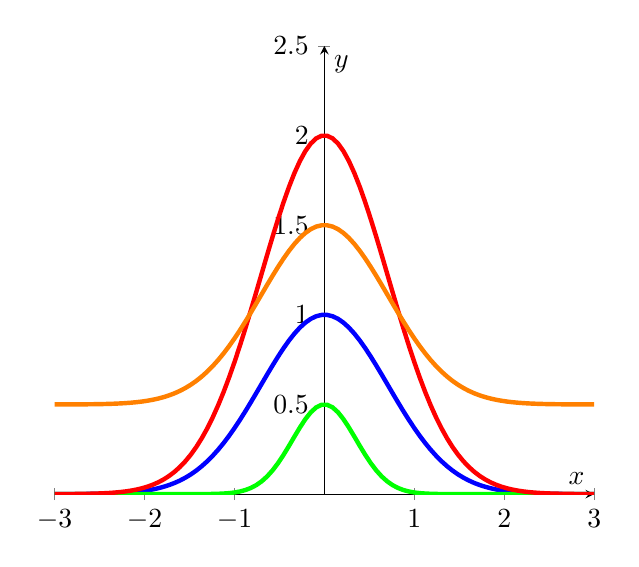
\begin{tikzpicture}[scale=1.0]
        \begin{axis}[
            axis x line=middle,
            axis y line=middle,
            ymin=0,ymax=2.5,ylabel=$y$,
            xmin=-3,xmax=3,xlabel=$x$
            ]

            \addplot[domain=-3:3, blue, ultra thick, samples=100] {e^(-x^2)};
            \addplot[domain=-3:3, green, ultra thick, samples=100] {0.5*e^(-(2*x)^2)};
            \addplot[domain=-3:3, red, ultra thick, samples=100] {2*(e^(-x^2))};
            \addplot[domain=-3:3, orange, ultra thick, samples=100] {e^(-x^2) + 0.5};
        \end{axis}
    \end{tikzpicture}
\caption{Amplitude transformations}
\label{fig:amplitude-scale-shifts}
\end{figure}

Given a signal $f(t)$, $f(at)$ will \emph{scale} the time domain by a factor of $\frac{1}{a}$, while $f(t - b)$ will \emph{shift} the time domain by $b$. Note that the opposite transformation is applied to the signal than is directly applied to the function inputs. Figure \ref{fig:time-scale-shifts} shows a signal $f(t)$ in blue, as well as:
\begin{itemize}
    \item $f(2t)$ in red,
    \item $f(\frac{t}{2})$ in green,
    \item and $f(t - 1)$ in orange.
\end{itemize}

It is important to note the different between scaling and then shifting the time of the signal, versus shifting and then scaling. Figure \ref{fig:time-scale-shifts-2} shows a signal $f(t)$ in blue, as well as:
\begin{itemize}
    \item $f(2(t-1))$ in red,
    \item and $f(2t-1)$ in green.
\end{itemize}

\begin{figure}[ht!]
    \centering
    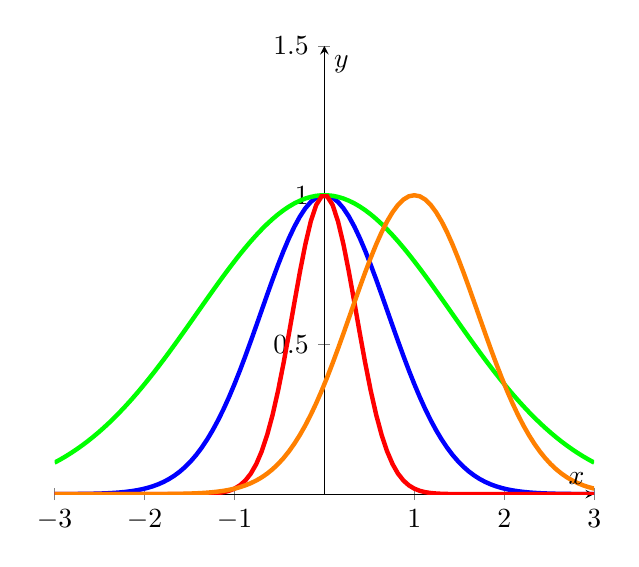
\begin{tikzpicture}[scale=1.0]
        \begin{axis}[
            axis x line=middle,
            axis y line=middle,
            ymin=0,ymax=1.5,ylabel=$y$,
            xmin=-3,xmax=3,xlabel=$x$
            ]

            \addplot[domain=-3:3, blue, ultra thick, samples=100] {e^(-x^2)};
            \addplot[domain=-3:3, green, ultra thick, samples=100] {e^(-(x/2)^2)};
            \addplot[domain=-3:3, red, ultra thick, samples=100] {(e^(-(2*x)^2))};
            \addplot[domain=-3:3, orange, ultra thick, samples=100] {e^(-(x-1)^2)};
        \end{axis}
    \end{tikzpicture}
\caption{Time transformations}
\label{fig:time-scale-shifts}
\end{figure}

\begin{figure}[ht!]
    \centering
    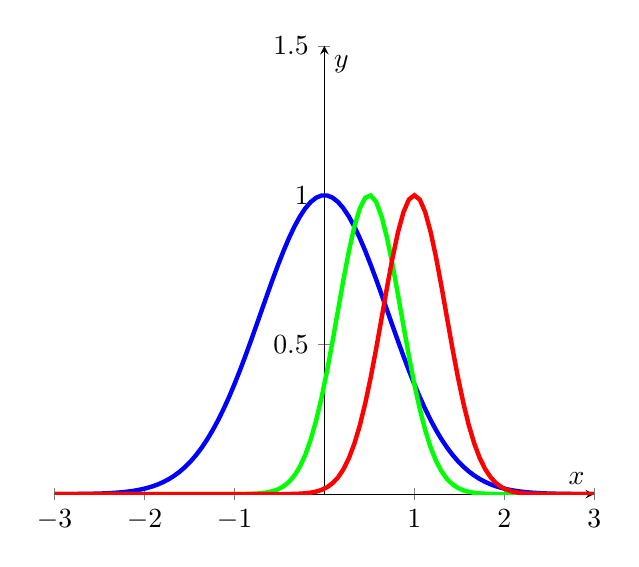
\begin{tikzpicture}[scale=1.0]
        \begin{axis}[
            axis x line=middle,
            axis y line=middle,
            ymin=0,ymax=1.5,ylabel=$y$,
            xmin=-3,xmax=3,xlabel=$x$
            ]

            \addplot[domain=-3:3, blue, ultra thick, samples=100] {e^(-x^2)};
            \addplot[domain=-3:3, green, ultra thick, samples=100] {e^(-(2*x-1)^2)};
            \addplot[domain=-3:3, red, ultra thick, samples=100] {e^(-(2*(x-1))^2};
        \end{axis}
    \end{tikzpicture}
\caption{Time transformations 2}
\label{fig:time-scale-shifts-2}
\end{figure}

\section{Common signals}

Two of the most common signals are the unit impulse signal, and the unit step signal. The unit impulse is also known as the (Dirac) delta function. In discrete time it is commonly denoted by $\delta[n]$, and is defined by
\[\delta[n] =
\begin{dcases}
    1, & n = 1 \\
    0, & n \neq 0
\end{dcases}.\] The unit step signal $u[n]$ is defined by
\[u[n] = \sum_{m=-\infty}^{n}\delta[m].\] Note that $\delta[n] = u[n] - u[n-1]$.

\begin{figure}[ht!]
    \centering
    \begin{tikzpicture}[scale=1.0]
        \begin{axis}[
            axis x line=middle,
            axis y line=middle,
            ymin=0,ymax=1.5,ylabel=$y$,
            xmin=-3,xmax=3,xlabel=$x$
            ]

            \addplot+[const plot, no marks, ultra thick] coordinates {(-3,0) (0,0) (0,1) (0,0) (3,0)};
        \end{axis}
    \end{tikzpicture}
\caption{Discrete unit impulse signal}
\label{fig:discrete-unit-impulse}
\end{figure}

\begin{figure}[ht!]
    \centering
    \begin{tikzpicture}[scale=1.0]
        \begin{axis}[
            axis x line=middle,
            axis y line=middle,
            ymin=0,ymax=1.5,ylabel=$y$,
            xmin=-3,xmax=3,xlabel=$x$
            ]

            \addplot+[const plot, no marks, ultra thick] coordinates {(-3,0) (0,0) (0,1) (3,1)};
        \end{axis}
    \end{tikzpicture}
\caption{Discrete unit step signal}
\label{fig:discrete-unit-step}
\end{figure}

The delta function can be used to sift out everything but one value of a discrete time signal.
\[x[n]\delta[n-n_0] = x[n_0]\delta[n-n_0]\]
\[\sum_{m=-\infty}^n x[m]\delta[m-n_0] = x[n_0]\]

In continuous time, we can define the unit step function similarly as \[u(t) =
\begin{dcases}
    1, & t > 0 \\
    0, & t < 0
\end{dcases}.\]
Note that $u(0)$ is undefined. Defining the continuous time impulse is a bit more challenging. We would like it to be $\delta(t)$ such that
\[u(t) = \int_{-t}^{t}\delta(\tau)d\tau.\] We can therefore define it has $\delta(t) = \lim_{\Delta\to 0}\delta_{\Delta}(t)$, where $\delta_{\Delta}(t)$ is a step impulse with width $\Delta$ and height $\frac{1}{\Delta}$ beginning at $t = 0$.

Note the similarities between the discrete and continuous time version of these signals -- the first difference and first derivative play the same roles, as do the sums and integrals.

\section{Energy and power}

\begin{defn}
    Let $x(t)$ be a continuous time signal. The \emph{energy} of the signal is
    \[E_{\infty} = \lim_{T\to\infty}\int_{-T}^{T}\abs{x(t)}^2dt.\]
\end{defn}

\begin{defn}
    Let $x(t)$ be a continuous time signal. The \emph{power} of the signal is
    \[P_{\infty} = \lim_{T \to \infty}\frac{1}{2T}\int_{-T}^T\abs{x(t)}^2dt.\]
\end{defn}

\begin{defn}
    Let $x[n]$ be a discrete time signal. The \emph{energy} of the signal is
    \[E_{\infty} = \lim_{N\to\infty}\sum_{n=-N}^{N}\abs{x[n]}^2.\]
\end{defn}

\begin{defn}
    Let $x[n]$ be a discrete time signal. The \emph{power} of the signal is
    \[P_{\infty} = \lim_{N \to \infty}\frac{1}{2N+1}\sum_{n=-N}^N\abs{x[n]}^2.\]
\end{defn}

Note that if a signal has finite energy, then the signal must approach zero sufficiently fast as time approaches $\pm\infty$, or equal zero outside some interval.

\begin{defn}
    An \emph{energy signal} is a signal with finite energy. Such signals must have zero power.
\end{defn}

\begin{exmp}
    $x(t) = e^{-\abs{t}}$ is an energy signal.
\end{exmp}

\begin{defn}
    A \emph{power signal} is a signal with finite, non-zero power. Such signals must have infinite energy.
\end{defn}

\begin{exmp}
    $x(t) = 1$ is a power signal, as is $x(t) = \sin(t)$.
\end{exmp}

Some signals are neither energy nor power signals, such as $x(t) = e^t$ or $x(t) = t$.

\begin{exmp}
    Let $x(t) = e^{-at}u(t)$ for some $a > 0$.
    \[E_{\infty} = \int_{-\infty}^{\infty}\abs{x(t)}^2dt = \int_{0}^{\infty}e^{-2at}dt = \frac{1}{-2a}(0 - 1) = \frac{1}{2a}.\] Since $a > 0$, $x(t)$ is therefore an energy signal and has zero power.
\end{exmp}

\begin{exmp}
    Let $x(t) = u(t)$. Then we have
    \[P_{\infty} = \lim_{T\to\infty}\frac{1}{2T}\int_{-T}^{T}\abs{x(t)}^2dt = \lim_{T\to\infty}\frac{1}{2T}\int_{0}^{T}dt = \frac{1}{2}.\] Therefore, $x(t)$ is a power signal and has infinite energy.
\end{exmp}

\section{Even and odd}

Recall that a function $f$ is even if $f(x) = f(-x)$ for all $x$ and odd if $f(x) = -f(-x)$. Obviously most functions are neither, but all functions can be decomposed into the sum of an even and odd part.

\begin{defn}
    Let $f(x)$ be a function, such as a signal. The \emph{even part} of $f$ is \[f_{\mathrm{ev}}(x) = \frac{f(x) + f(-x)}{2},\] and the \emph{odd part} of $f$ is \[f_{\mathrm{od}}(x) = \frac{f(x) - f(-x)}{2}.\]
\end{defn}

Note that the even part of a function must be even, since \[f_{\mathrm{ev}}(-x) = \frac{f(-x) + f(x)}{2} = \frac{f(x) + f(-x)}{2} = f_{\mathrm{ev}}(x),\] and the odd part must be odd: \[-f_{\mathrm{od}}(-x) = \frac{-f(-x)+f(x)}{2} = \frac{f(x) - f(-x)}{2} = f_{\mathrm{od}}(x).\]

\begin{exmp}
    $5x^2$ is even, while $x^3$ is odd, but $f(x) = x^3 + 5x^2$ is neither. \[f_{\mathrm{ev}}(x) = \frac{(x^3 + 5x^2) + ((-x)^3) + 5(-x)^2)}{2} = \frac{(x^3 - x^3) + (5x^2 + 5x^2)}{2} = 5x^2.\]
    \[f_{\mathrm{od}}(x) = \frac{(x^3 + 5x^2) - ((-x)^3) + 5(-x)^2)}{2} = \frac{(x^3 + x^3) + (5x^2 - 5x^2)}{2} = x^3.\]
\end{exmp}

\begin{prop}
    Let $f(x)$ be a function. Then $f(x) = f_{\mathrm{ev}}(x) + f_{\mathrm{od}}(x)$.
\end{prop}

\begin{proof}
    \begin{align*}
        f_{\mathrm{ev}}(x) + f_{\mathrm{od}}(x) &= \\
        \frac{f(x) + f(-x)}{2} + \frac{f(x) - f(-x)}{2} &= \\
        \frac{f(x) + f(-x) + f(x) - f(-x)}{2} &= \\
        \frac{2f(x)}{2} = f(x)
    \end{align*}
\end{proof}

\section{Period and frequency}

\begin{defn}
    A signal $x(t)$ is \emph{bounded} if there exists some $K$ such that $\abs{x(t)} < K$ for all $t$.
\end{defn}

\begin{defn}
    A signal $x(t)$ is \emph{periodic} if there exists some $T \in \R$ such that $x(t) = x(t + T)$ for all $T$. Note that if $f(t)$ is periodic with period $T$, it must also be periodic with period $kT$ where $k \in \Z^+$. The smallest such $T$ is called $T_0$, the \emph{fundamental period}.
\end{defn}

\begin{rmk}
    For discrete time signals, it is instead required that $T \in \Z^+$.
\end{rmk}

\begin{rmk}
    Constant signals are somewhat of an edge case with respect to periodicity. They are clearly periodic for any period $T > 0$, but have no fundamental period, and hence no fundamental frequency.
\end{rmk}

\begin{defn}
    Given that $x(t)$ is periodic with fundamental period $T_0$, the \emph{fundamental frequency} of $x(t)$ is $\omega_0 = \frac{2\pi}{T_0}$. Some sources instead call $f_0$ the fundamental frequency where $f_0 = \frac{1}{T_0}$.
\end{defn}

\begin{exmp}
    Let $x(t) = \sin(3t)$. If $x(t)$ is periodic with some period $T$, then it must be that $x(t) = x(t + T)$, so $\sin(3t) = \sin(3(t + T)) = \sin(3t + 3T)$. We know that $\sin$ is periodic with fundamental period $2\pi$, so $3T_0 = 2\pi$ and therefore $T_0 = \frac{2\pi}{3}$.
\end{exmp}

\begin{exmp}
    Let $x(t) = e^{\pi(1 + j)t}$. Then we have $x(t) = x(t + T)$ which implies \[e^{\pi(1 + j)t} = e^{\pi(1 + j)(t + T)} = e^{\pi(1 + j)t}e^{\pi(1 + j)T}.\] Since $e^x \neq 0$ for all $x$, it follows that $e^{\pi(1 + j)T} = 1$, and so it must be that $\pi(1 + j)T = 2k{\pi}$ for some $k \in \Z$ by Euler's formula. Therefore, $T = \frac{2k}{1 + j}$. However, $T \notin \R$, so $x(t)$ is not periodic.
\end{exmp}

\begin{rmk}
    If a \emph{non-zero} signal is both \emph{periodic} and \emph{bounded}, it must be a power signal.
\end{rmk}

\begin{rmk}
    Signals which are periodic in continuous time may not be in discrete time. For example, we saw that $x(t) = \sin(3t)$ is periodic, but $x[n] = \sin(3n)$ is not, as there is no $N \in \Z^+$ such that $N = \frac{2\pi}{3}$.
\end{rmk}

\section{Exponential signals}

\subsection{Continuous time}

\begin{defn}
    An \emph{exponential signal} is a signal of the form $x(t) = ce^{at}$, for some $c, a \in \C$ and $t \in \R$.
\end{defn}

When $c, a \in \R$, the exponential signal is similar to the standard exponential function. If $a > 0$, the signals grows exponentially, if $a < 0$ it decreases exponentially, and in any case it is scaled by $c$.

When $c \in \C$ and $a$ is strictly imaginary, the signal is called a \emph{phasor}. By Euler's formula, we have \[ce^{at} = \abs{c}e^{i\phi_0}e^{at} = \abs{c}e^{i(\omega_0t + \phi_0)} = \abs{c}\left(\cos(\omega_0t + \phi_0) + i\sin(\omega_0t + \phi_0)\right),\] where $i\omega_0 = a$ and $\phi_0 = \angle c$. A phasor can be interpreted as a vector-valued function, which always have magnitude $\abs{c}$, and has angular frequency $\omega_0$ (radians/time). At time $t = 0$, the angle is $\phi_0$, which may be called the \emph{phase} of the signal. Since the signal has angular frequency $\omega_0$, it has fundamental period $T_0 = \frac{2\pi}{\abs{w_0}}$.

\begin{thm}
    Let $x(t) = c_1e^{i\omega_1t} + c_2e^{i\omega_2t}$. This signal is periodic if and only if there exists some $\omega > 0$ and $k_1, k_2 \in \Z$ such that $\omega_1 = k_1\omega$ and $\omega_2 = k_2\omega$. If it is periodic, it has fundamental period $T_0 = \frac{2\pi}{\omega_0}$, where $\omega_0$ is the largest possible value for $\omega$.
\end{thm}

\begin{rmk}
    The required condition is equivalent to $\frac{\omega_1}{\omega_2} \in \Q$. Note that this theorem can be generalized to signals that are the sum of $n$ phasors.
\end{rmk}

\begin{exmp}
    Let $x(t) = 4e^{i2t} - 5e^{i3t}$. Since $2 = 2\cdot 1$ and $3 = 3 \cdot 1$, $x(t)$ is periodic with fundamental frequency $w_0 = 1$ and fundamental period $T_0 = \frac{2\pi}{\abs{1}} = 2\pi$.
\end{exmp}

\begin{exmp}
    Let $x(t) = 4e^{i2t} - 5e^{i\pi t}$. Since $\frac{2}{\pi} \not\in \Q$, $x(t)$ is not periodic.
\end{exmp}

\begin{defn}
    If a signal $x(t) = c_1e^{i\omega_1t} + c_2e^{i\omega_2t} + \cdots + c_ke^{i\omega_kt}$ is periodic, then we say the terms are \emph{harmonically related}.
\end{defn}

When $c, a \in \C$, and $a$ is not strictly imaginary, then the resulting exponential signal is a phasor given by $c$ and the imaginary part of $a$, all multiplied by $e^{\sigma_0}$, where $\sigma_0$ is the real part of $a$.

\subsection{Discrete time}

\begin{defn}
    An \emph{exponential signal} is a signal of the form $x[n] = ce^{an}$, for some $c, a \in \C$ and $n \in \N$.
\end{defn}

When $c, a \in \R$, the exponential signal is similar to the standard exponential function. If $a > 0$, the signals grows exponentially, if $a < 0$ it decreases exponentially, and in any case it is scaled by $c$.

When $c \in \R$ and $a = \sigma_0 + i(2k+1)\pi$ for some $\sigma_0 \in \R$ and $k \in \Z$, we have a type of exponential signal that doesn't have a continuous time version. Since $x[n] = ce^{an}$, we have $x[n] = c\left(-e^{\sigma_0}\right)^n$. This signal therefore is simply $ce^{n\sigma_0}$, but alternating between positive and negative on each sample.

When $c \in \C$ and $a$ is strictly imaginary, the signal is a discrete time \emph{phasor}. Unlike continuous time phasors, discrete time phasors are not always periodic. For $x[n] = e^{i\omega_0n}$ to be periodic in discrete time, we need $\frac{2\pi}{\abs{\omega_0}} \in \Q$, so that some integer multiple of this value is an integer period.

\begin{thm}
    Let $x[n] = c_1e^{i\omega_1n} + c_2e^{i\omega_2n}$, where the terms are periodic with fundamental periods $N_1, N_2 \in \N$. This signal is then periodic, and has fundamental period equal to the least common multiple of $N_1$ and $N_2$.
\end{thm}

\begin{rmk}
    Note that this theorem can be generalized to signals that are the sum of $n$ discrete time phasors.
\end{rmk}

\begin{rmk}
    For a continuous time phasors, increasing $\omega_0$ always results in a phasor with higher frequency. For a discrete time phasor however, add integer multiples of $2\pi$ to $\omega_0$ least the phasor unchanged.
\end{rmk}

\end{document}

\setchaptergraphic{}

\chapter{Mathematics of Images and Shapes}
\label{ch:images}

\section{Images}

\subsection{Mathematically Describing Images}

Traditionally, images have been modeled as graphs (or level sets) of continuous functions defined on a rectangular domain $D \subset \R^2$, and codomain $P \subset \R$. That is, an image $f$ with domain $D$ and codomain $P$ is \[D = \left[0, R_1\right] \times \left[0, R_2\right] \subset \R^2,\] \[P = \left[0, L\right] \subset \R,\] \[f : D \to P.\]

This definition is for grayscale (black and white), images, not color images. A value of $0$ would correspond to the color black, and $L$ to white, and everything in between would be various shades of gray.

To perform computational work with images, it is useful to discretize images. This can be done by sampling the functions at $(m, n)$ for all $m \in \{0, \ldots, M-1\}$ and $n \in \{0, \ldots, N-1\}$ where $M$ and $N$ are the number of pixels on the $y$-axis and $x$-axis respectively. $L$ is chosen to be $2^b-1$ where $b$ is the number of bits per pixel. We can then discretize the domain into $\mathbb{P} = \{0, \ldots, 2^b-1\}$. Discretized images are the graph of a discrete function $I: \mathbb{D} \to \mathbb{P}$, where $\mathbb{D} = \{0, \ldots, M-1\} \times \{0, \ldots, N-1\}$. This can be represented as an $M \times N$ matrix $I(i, j)$ where $(i, j) \in \mathbb{D}$.

Color images can be represented as three of these matrices (or a single three-dimensional matrix), each corresponding to one dimension of a color space, such as RGB or HSV.

\subsection{Point Operations}

\begin{defn}
    Given a mapping $T: \mathbb{P} \to \mathbb{P}$, a \emph{point operation} on an image $I: \mathbb{D} \to \mathbb{P}$ is defined as $J(i, j) = T(I(i, j))$ for all $(i, j) \in \mathbb{D}$.
\end{defn}

\begin{rmk}
    $J(i, j)$ depends only on $I(i, j)$, not on any other pixel.
\end{rmk}

\begin{defn}
    The \emph{Heaviside function} is $H: \R \to \R$, where $H(x) = \left\{
    \begin{array}{lr}
        1 & : x \geq 0 \\
        0 & : x < 0
    \end{array}\right.$
\end{defn}

\begin{figure}[ht!]
    \centering
    \begin{tikzpicture}[scale=1.0]
        \begin{axis}[
            axis x line=middle,
            axis y line=middle,
            ymin=0,ymax=256,ylabel=$y$,
            xmin=0,xmax=256,xlabel=$x$
        ]
            \addplot[domain=0:100, blue, ultra thick] {0};
            \addplot[domain=100:256, blue, ultra thick] {255};
            \addplot[color=blue,fill=white,only marks,mark=*] coordinates{(100,0)};
            \addplot[color=blue,only marks,mark=*] coordinates{(100,255)};
        \end{axis}
    \end{tikzpicture}
\caption{Graph of threshold function $(L-1)H(r - t)$ where $L = 256$ and $t = 100$.}
\label{fig:threshold}
\end{figure}

\begin{figure}[ht!]
    \centering
    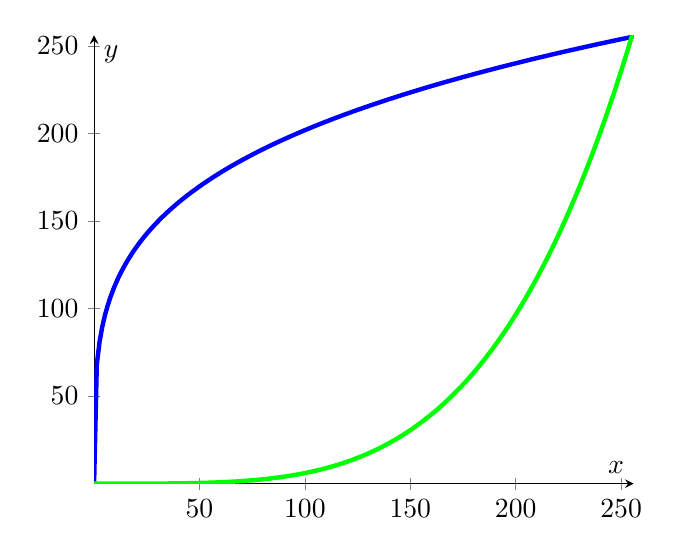
\begin{tikzpicture}[scale=1.0]
        \begin{axis}[
            axis x line=middle,
            axis y line=middle,
            ymin=0,ymax=256,ylabel=$y$,
            xmin=0,xmax=256,xlabel=$x$
            ]
        \addplot[domain=0:256, blue, ultra thick, samples=200] {255*(x/255)^0.25};
        \addplot[domain=0:256, green, ultra thick, samples=200] {255*(x/255)^4.0};
    \end{axis}
    \end{tikzpicture}
\caption{Graph of gamma function $(L-1)\left(\frac{r}{L-1}\right)^\gamma$ where $\gamma = 4$ (green) and $\gamma = \frac{1}{4}$ (blue).}
\label{fig:gamma}
\end{figure}

\begin{figure}[ht!]
    \centering
    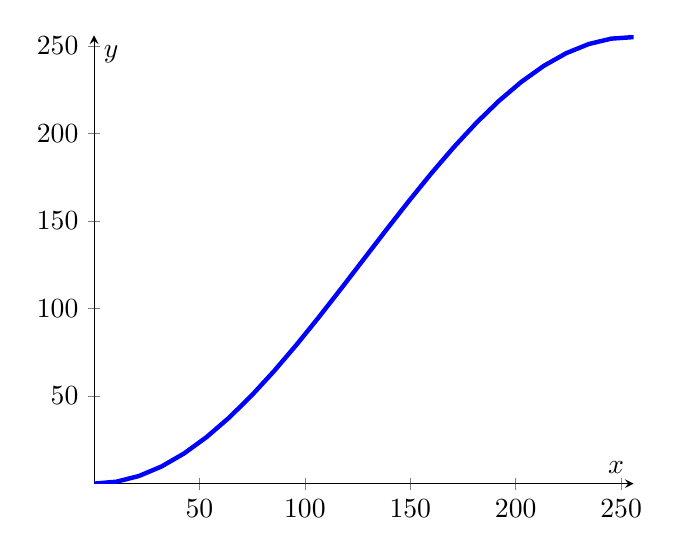
\begin{tikzpicture}[scale=1.0]
        \begin{axis}[
            axis x line=middle,
            axis y line=middle,
            ymin=0,ymax=256,ylabel=$y$,
            xmin=0,xmax=256,xlabel=$x$
            ]
        \addplot[domain=0:256, blue, ultra thick] {127.5 + 127.5*sin(deg(0.5*pi*(x - 127.5)/127.5))};
    \end{axis}
    \end{tikzpicture}
\caption{Graph of contrast enhancement $c + c\sin\left(\frac{\pi(r-c)}{2c}\right)$.}
\label{fig:contrast}
\end{figure}

For the following four examples, let $I = \begin{bmatrix}
    0 & 0 & 0\\ 255 & 255 & 0 \\ 255 & 0 & 100
\end{bmatrix}$, so $\mathbb{D} = \left[0, 2\right] \times \left[0, 2\right]$, and let $L = 2^8 = 256$ so $\mathbb{P} = \left[0, 256 - 1\right]$.

\begin{exmp}
    Identity: $T: r \mapsto r$, $J = \begin{bmatrix}
        0 & 0 & 0\\ 255 & 255 & 0 \\ 255 & 0 & 100
    \end{bmatrix}$.
\end{exmp}

\begin{exmp}
    Negative: $T: r \mapsto (L-1) - r$, $J = \begin{bmatrix}
        255 & 255 & 255 \\ 0 & 0 & 255 \\ 0 & 255 & 155
    \end{bmatrix}$.
\end{exmp}

\begin{exmp}
    Converting a grayscale image to B\&W uses a threshold function, an example of which is shown in Figure \ref{fig:threshold}. \[T: r \mapsto (L-1)H(r - t)\] where $L \geq t \geq 0$. \[J = \begin{bmatrix}
        0 & 0 & 0\\ 255 & 255 & 0 \\ 255 & 0 & 0
    \end{bmatrix}\]
\end{exmp}

\begin{exmp}
    Gamma-correction uses the gamma function, two examples of which are shown in Figure \ref{fig:gamma}. \[T: r \mapsto (L-1)\left(\frac{r}{L-1}\right)^\gamma\] where $\gamma > 0$. When $\gamma > 1$ the image is darkened, when $\gamma < 1$ the image is brightened, and when $\gamma = 1$ the image is unchanged.
\end{exmp}

\begin{exmp}
    Contrast-enhancement can be done using the function shown in Figure \ref{fig:contrast}. \[T: r \mapsto c + c\sin\left(\frac{\pi(r-c)}{2c}\right)\] where $c = \frac{L - 1}{2}$. When $\gamma > 1$ the image is darkened, when $\gamma < 1$ the image is brightened, and when $\gamma = 1$ the image is unchanged.
\end{exmp}

\subsection{Filtering and Convolutions}

\begin{defn}
    A \emph{filter mask} $w$ is a $(2k_1 + 1) \times (2k_2 + 1)$ matrix, where $k_1, k_2 \in \N$.

    \[w = \begin{bmatrix}
        w{(-k_1, -k_2)} & \cdots & w{(-k_1, 0)} & \cdots & w{(-k_1, k_2)} \\
        \vdots & \ddots & \vdots & \iddots & \vdots \\
        w{(0, -k_2)} & \cdots & w{(0, 0)} & \cdots & w{(0, k_2)} \\
        \vdots & \iddots & \vdots & \ddots & \vdots \\
        w{(k_1, -k_2)} & \cdots & w{(k_1, 0)} & \cdots & w{(k_1, k_2)} \\
    \end{bmatrix}\]
\end{defn}

\begin{exmp}
    A \emph{mean} or \emph{uniform averaging} filter uses a filter mask where
    \[w = \frac{1}{k_1k_2}\begin{bmatrix}
        1 & \cdots & 1 & \cdots & 1 \\
        \vdots & \ddots & \vdots & \iddots & \vdots \\
        1 & \cdots & 1 & \cdots & 1 \\
        \vdots & \iddots & \vdots & \ddots & \vdots \\
        1 & \cdots & 1 & \cdots & 1 \\
    \end{bmatrix}.\] Typically, averaging filters are used with a $3 \times 3$ or $5 \times 5$ mask.
\end{exmp}

\begin{exmp}
    A \emph{Gaussian} filter uses a filter mask created by sampling a Gaussian function \[g(x, y) = \frac{1}{2\pi\sigma^2}e^{-\frac{x^2+y^2}{2\sigma^2}}\] where
    \[w = \begin{bmatrix}
        g(-k_1, -k_2) & \cdots & g(-k_1, 0) & \cdots & g(-k_1, k_2) \\
        \vdots & \ddots & \vdots & \iddots & \vdots \\
        g(0, -k_2) & \cdots & g(0, 0) & \cdots & g(0, k_2) \\
        \vdots & \iddots & \vdots & \ddots & \vdots \\
        g(k_1, -k_2) & \cdots & g(k_1, 0) & \cdots & g(k_1, k_2) \\
    \end{bmatrix}.\]
\end{exmp}

\begin{defn}
    Let $I: \mathbb{D} \to \mathbb{P}$ be an image, and $w$ a filter mask. Then applying the \emph{filter} represented by $w$ to $I$ results in the image $J: \mathbb{D} \to \mathbb{D}$ defined by: \[J(i, j) = \sum_{u = -k_1}^{k_1}\sum_{v = -k_2}^{k_2}I(i + u, j + v)w(u, v).\]
\end{defn}

Notice that filters cannot be naively applied to the $k_1 + 1$ top/bottom-most rows, nor the $k_2 + 1$ left/right-most columns of $I$, since entries with indices outside the image do not exist. This problem can be solved via a variety of strategies.
\begin{itemize}
    \item One option is to zero-pad the image. For example, if $I$ is $3 \times 3$, then $I(2, 3)$ and $I(-1, 2)$ would both be $0$.
    \item Zero-padding a bright image could cause strange filter behavior near the edges, so the image could instead be padded with the average value of the entire image.
    \item Constant-padding with the average could still cause issues if parts of the image's edges differ significantly from the rest of the image, so nearest-neighbor padding can be used instead. This is where the added padding pixels have the same value as the nearest pixel from the image.
    \[\begin{array}{c c||c c c}
        3 & 3 & 3 & 7 & 2 \\
        3 & 3 & 3 & 7 & 2\\
        \hline \hline
        3 & 3 & 3 & 7 & 2 \\
        5 & 5 & 5 & 1 & 6 \\
        8 & 8 & 8 & 9 & 4 \\
    \end{array}\]
    \item Nearest-neighbor can cause issues with detecting edges that are near/coincide with the edge of the image itself. This can be solved by instead by using reflective (also symmetric)padding. The reflection of the image's outer rows/columns can help accentuate an edge if one exists, rather than suppressing it like nearest-neighbor.
    \[\begin{array}{c c||c c c}
        1 & 5 & 5 & 1 & 6 \\
        7 & 3 & 3 & 7 & 2\\
        \hline \hline
        7 & 3 & 3 & 7 & 2 \\
        1 & 5 & 5 & 1 & 6 \\
        9 & 8 & 8 & 9 & 4 \\
    \end{array}\]
    \item Periodic padding tiles the image, so accessing entries past one side will wrap around and access entries on the other side. Can be useful if images can an inherent periodicity that reflective padding doesn't take advantage of.
\end{itemize}

\begin{defn}
    Let $I: \Z^2 \to \R$ be a function representing an image $I_0: \mathbb{D} \to \mathbb{P}$ take has been extended to infinity by zero-padding. Note that $I_0$ could be another image that has been padded in some way. Let $h: \Z^2 \to \R$ be a function (called the \emph{kernel} or \emph{convolution kernel}). Then we define the \emph{convolution} of $I$ and $h$, denoted by $I * h$, as \[(I * h)(i, j) = \sum_{k=-\infty}^{\infty}\sum_{l=-\infty}^{\infty}I(i - k, j - l)(h, k, l).\] Notice the similarities to the definition of applying a filter, and the differences --- there on no bounds, and the image entries are indexed using $i - k$ and $i - l$ rather than $i + u$ and $i + v$.
\end{defn}

Filtering can be defined in terms of convolution. To apply a $(2k_1 + 1) \times (2k_2 + 1)$ filter mask $w$ to an $n \times m$ image $I$ (which may be padded), define $h(k, l) = w(-k, l)$, and extend both $h$ and $I$ to infinity by zero-padding. Then $J = I * H$.

\begin{exmp}\proofbreak
    \begin{itemize}
        \item The mean filter mask can be used as a convolution kernel to evenly blur images, smoothing them out and removing noise.
        \item The Gaussian blurring can be performed by using the Gaussian mask as a convolution kernel, resulting in less significant smoothing effects while still working to denoise the image.
    \end{itemize}
\end{exmp}

Convolution is a linear operation, however several useful filtering operations are non-linear. One example is median blurring. Similarly to how mean filtering defines $J(i, j)$ to be the mean of the neighborhood of $I(i, j)$, median blurring uses the median of the neighborhood of $I(i, j)$. This can result in superior denoising, while better preserving edges. However, it is more computationally expensive than either mean or Gaussian blurring.

\subsection{Partial Derivatives for Images}

\begin{defn}
    When $\Delta x$ is small enough, $f'(x_0)$ can be approximated using the \emph{forward difference formula}: \[f'(x_0) \approx \frac{f(x_0 + \Delta x) - f(x_0)}{\Delta x}.\]
\end{defn}

\begin{defn}
    When $\Delta x$ is small enough, $f'(x_0)$ can be approximated using the \emph{back difference formula}: \[f'(x_0) \approx \frac{f(x_0) - f(x_0 - \Delta x)}{\Delta x}.\]
\end{defn}

\begin{rmk}
    Often, for a particular function at a particular point, the forward difference formula will overestimate the derivative and the backward difference formula will underestimate it, or vice versa. Thus, the average often gives a better approximation.
\end{rmk}

\begin{defn}
    The \emph{central difference formula} (also the \emph{midpoint formula)} approximates $f'(x_0)$ for a function $f$ as the average of the forward and backward difference functions. \[f'(x_0) \approx \frac{1}{2}\left(\frac{f(x_0 + \Delta x) - f(x_0)}{\Delta x} + \frac{f(x_0) - f(x_0 - \Delta x)}{\Delta x}\right) = \frac{f(x_0 + \Delta x) - f(x_0 - \Delta x)}{2\Delta x}.\]
\end{defn}

\begin{rmk}
    We can approximate the second derivative $f''(x_0)$ of a function $f$ at point $x_0$ as \[f''(x_0) \approx \frac{f(x_0 + \Delta x) - 2f(x_0) + f(x_0 - \Delta x)}{\left(\Delta x\right)^2}\] by applying the forward difference formula to the backward difference formula or vice versa.
\end{rmk}

\begin{defn}
    These approximations of derivatives are known as \emph{finite differences}.
\end{defn}

\begin{exmp}
    Let $f: D \subseteq \R^2 \to \R$ be a function. We can use the central difference formula to approximate the first and second partial derivatives of $f(x, y)$ at $(x_0, y_0) \in \mathbb{D}$.

    \[\frac{\partial f}{\partial x}(x_0, y_0) \approx \frac{f(x_0 + \Delta x, y_0) - f(x_0 - \Delta x, y_0)}{2\Delta x}.\]

    \[\frac{\partial f}{\partial y}(x_0, y_0) \approx \frac{f(x_0, y_0  + \Delta y) - f(x_0, y_0 - \Delta y)}{2\Delta y}.\]

    \[\frac{\partial^2 f}{\partial x^2}(x_0, y_0) \approx \frac{f(x_0 + \Delta x, y_0) - 2f(x_0, y_0) + f(x_0 - \Delta x, y_0)}{\left(\Delta x\right)^2}.\]
\end{exmp}

\begin{rmk}
    To apply these formulas to images, we have $x_0 = j$, $y_0 = i$, and $\Delta x = \Delta j = 1$, $\Delta y = \Delta i = 1$.
\end{rmk}

\begin{exmp}
    Let $I: \mathbb{D} \to \mathbb{P}$ be an image. Then the following are approximations of the derivatives of $I$ at $(i, j) \in \mathbb{D}$:
    \[\frac{\partial^2I}{\partial y^2}(i, j) \approx \frac{I(i + 1, j) - 2I(i, j) + I(i - 1, j)}{1^2},\]
    \[\frac{\partial I}{\partial y}(i, j) \approx \frac{I(i + 1, j) - I(i - 1, j)}{2},\]
    \[\frac{\partial I}{\partial x}(i, j) \approx \frac{I(i, j + 1) - I(i, j - 1)}{2},\]
\end{exmp}

Since $\frac{\partial I}{\partial y}(i, j) \approx \frac{I(i + 1, j) - I(i - 1, j)}{2} = \frac{1}{2}I(i + 1, j) - \frac{1}{2}I(i - 1, j)$ for some image $I: \mathbb{D} \to \mathbb{P}$, we can find $\frac{\partial I}{\partial y}$ for every $(i, j) \in \mathbb{D}$ by filtering $I$ with the filter mask \[w_y = \begin{bmatrix}
    0 & -1/2 & 0 \\
    0 & 0 & 0 \\
    0 & 1/2 & 0 \\
\end{bmatrix}.\] This is equivalent to the convolution $I * h_y$, where \[h_y = \begin{bmatrix}
    0 & 1/2 & 0 \\
    0 & 0 & 0 \\
    0 & -1/2 & 0 \\
\end{bmatrix}.\]

In practice, the Prewitt or Sobel filters are much more frequently used.

Prewitt filter: \[w_y^P = \frac{1}{6}\begin{bmatrix}
    -1 & -1 & 1 \\
    0 & 0 & 0 \\
    1 & 1 & 1 \\
\end{bmatrix}\]

Sobel filter: \[w_y^S = \frac{1}{8}\begin{bmatrix}
    -1 & -2 & -1 \\
    0 & 0 & 0 \\
    1 & 2 & 1 \\
\end{bmatrix}\]

The Prewitt filter uses the average of three adjacent first derivatives in order to smooth out noise, and the Sobel filter does the same, but with a weighted average.

\subsection{Laplacian for Images}

\begin{defn}
    Let $f: \R^n \to \R$ be a twice-differentiable function. The \emph{Laplacian} of $f$ is the sum of all unmixed second order partial derivatives.

    \[\nabla^2f(x_1, \ldots, x_n) = \sum_{i=1}^n \frac{\partial^2f}{\partial x_i^2}(x_1, \ldots, x_d)\]
\end{defn}

\begin{exmp}
    Let $f: \R^2 \to \R$. Then at some $(x_0, y_0) \in \R^2$, \[\nabla^2 f(x_0, y_0) = \frac{\partial^2f}{\partial x^2}(x_0, y_0) + \frac{\partial^2f}{\partial y^2}(x_0, y_0).\]
\end{exmp}

\begin{defn}
    Let $I: \mathbb{D} \to \mathbb{P}$ be an image. Then its \emph{Laplacian} is defined by \[\nabla^2I(i, j) = (I * h_{xx})(i, j) + (I * h_{xx})(i, j),\] where $h_xx$ and $h_yy$ are kernels for the approximation of the images second derivatives.
\end{defn}

Since convolution distributes over addition of kernels, \[(I * h_{xx})(i, j) + (I * h_{xx})(i, j) = \left(I * (h_{xx} + h_{xx}\right)(i, j).\] Let $h_L = h_{xx} + h_{yy}$, then
\[h_L = \begin{bmatrix}
    0 & 1 & 0 \\ 1 & -4 & 1 \\ 0 & 1 & 1
\end{bmatrix}.\]

The following kernels are more frequently used to practice, which they use a weighted average of adjacent values as with the Prewitt and Sobel filters:

\[h_{L_8} = \begin{bmatrix}
    1 & 1 & 1 \\ 1 & -8 & 1 \\ 1 & 1 & 1
\end{bmatrix}\]

\[h_{L_12} = \begin{bmatrix}
    1 & 2 & 1 \\ 2 & -12 & 2 \\ 1 & 2 & 1
\end{bmatrix}\]

The Laplacian of an image can be used to sharpen the image. For example, consider the logistic function, its first derivative, and its Laplacian, which are shown in Figure \ref{fig:laplacian} as the blue, green, and red graphs respectively.

\[f(x) = \frac{e^x}{e^x + 1}\]
\[\nabla{f} = \frac{e^x}{(e^x + 1)^2}\]
\[\nabla^2f(x) = \frac{e^x - e^{3x}}{(e^x + 1)^4}\]

\begin{figure}[ht!]
    \centering
    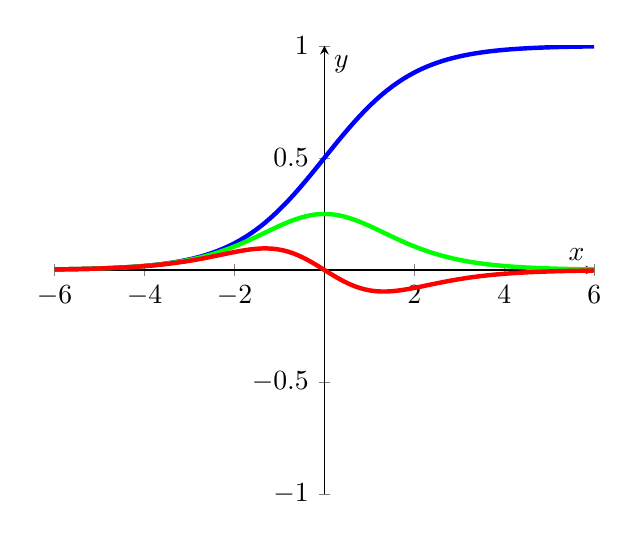
\begin{tikzpicture}[scale=1.0]
        \begin{axis}[
            axis x line=middle,
            axis y line=middle,
            ymin=-1,ymax=1,ylabel=$y$,
            xmin=-6,xmax=6,xlabel=$x$
            ]
        \addplot[domain=-6:6, blue, ultra thick, samples=100] {e^x/(e^x+1)};
        \addplot[domain=-6:6, green, ultra thick, samples=100] {e^x/(e^x+1)^2};
        \addplot[domain=-6:6, red, ultra thick, samples=100] {(e^x-e^(3*x))/(e^x+1)^4};
    \end{axis}
    \end{tikzpicture}
\caption{Graph of the logistic function, its first derivative, and its Laplacian.}
\label{fig:laplacian}
\end{figure}

Now consider the function $g(x) = f(x) - k\nabla^2f(x)$ for some positive real constant $k$. $g(x)$ for the logistic function with $k=2$ is shown in red in comparison to the logistic function in blue in Figure \ref{fig:laplacian-sharpening}. This technique will sharpen any twice-differentiable function, as it will essentially ``pull-down'' concave-down parts of the function, and ``push-up'' concave-up parts of the function. The effect of this is to accentuate corners and make regions are inflection points steeper.

\begin{figure}[ht!]
    \centering
    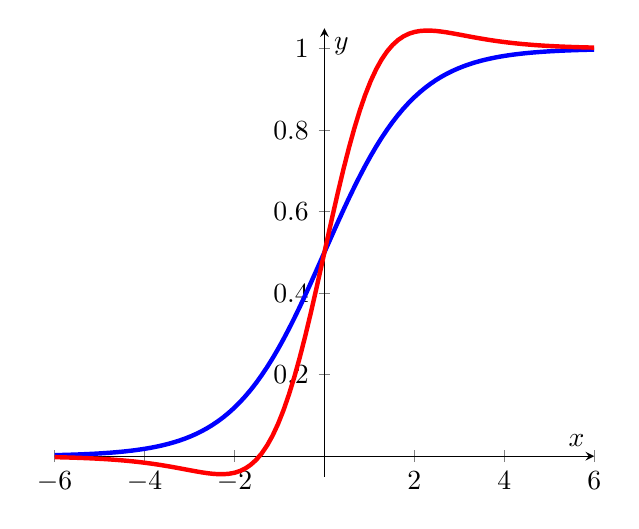
\begin{tikzpicture}[scale=1.0]
        \begin{axis}[
            axis x line=middle,
            axis y line=middle,
            ymin=-0.05,ymax=1.05,ylabel=$y$,
            xmin=-6,xmax=6,xlabel=$x$
            ]
        \addplot[domain=-6:6, blue, ultra thick, samples=100] {e^x/(e^x+1)};
        \addplot[domain=-6:6, red, ultra thick, samples=100] {e^x/(e^x+1) - 2*((e^x-e^(3*x))/(e^x+1)^4)};
    \end{axis}
    \end{tikzpicture}
\caption{Graph of $f(x) - k\nabla^2f(x)$, where $k=2$.}
\label{fig:laplacian-sharpening}
\end{figure}

We can apply this technique to an entire image. Let $I: \mathbb{D} \to \mathbb{P}$ be an image, then define $J$ by \[J(i, j) = I(i, j) - k\nabla^2I(i, j),\] for all $(i, j) \in \mathbb{D}$ and some real $k > 0$.

\subsection{Image Processing on Graphs}

We can apply graph theory and signal processing to image processing by modelling image data as graph signals. We will first define graphs and graph signals, and then explore how they can be applied to image processing.

\begin{defn}
    An \emph{undirected graph} is a $2$-tuple $\mathcal{G} = (\mathcal{V}, \mathcal{E})$, where $\mathcal{V}$ is a set of vertices, and $\mathcal{E}$ is a set of unordered pairs (two-sets) of vertices, called edges.
\end{defn}

\begin{defn}
    The \emph{adjacency matrix} $\bm{A}$ of a graph $\mathcal{G} = (\mathcal{V}, \mathcal{E})$ is a square $|\mathcal{V}| \times |\mathcal{V}|$ matrix where $\bm{A}_{i, j}$ is $1$ if there is an edge from $\mathcal{V}_i$ to $\mathcal{V}_j$, and $0$ otherwise.
\end{defn}

\begin{exmp}
    Let $\mathcal{V} = \{1, 2, 3, 4\}$, let $\mathcal{E} = \{\{1, 2\}, \{2, 3\}, \{3, 4\}, \{4, 1\}\}$. Then $\mathcal{G} = (\mathcal{V}, \mathcal{E})$ is the graph shown in Figure \ref{fig:example-graph}. The adjacency matrix of $\mathcal{G}$ is
    \[\bm{A} = \begin{bmatrix}
        0 & 1 & 0 & 1 \\
        1 & 0 & 1 & 0 \\
        0 & 1 & 0 & 1 \\
        1 & 0 & 1 & 0
    \end{bmatrix}.\]
\end{exmp}

\begin{figure}[ht!]
    \centering
    \begin{tikzpicture}
        \begin{scope}[every node/.style={circle,thick,draw,fill=cyan}]
            \node (1) at (0,0) {1};
            \node (2) at (2,0) {2};
            \node (3) at (2,2) {3};
            \node (4) at (0,2) {4};
        \end{scope}

        \begin{scope}[>={Stealth[black]},
            every node/.style={fill=white,circle},
            every edge/.style={draw=black,very thick}]
            \path [<->] (1) edge (2);
            \path [<->] (2) edge (3);
            \path [<->] (3) edge (4);
            \path [<->] (4) edge (1);
        \end{scope}
    \end{tikzpicture}
\caption{Example graph.}
\label{fig:example-graph}
\end{figure}

\begin{defn}
    A \emph{weighted, undirected graph} is a $3$-tuple $\mathcal{G} = (\mathcal{V}, \mathcal{E}, \bm{W})$, where $\mathcal{V}$ is a set of vertices, $\mathcal{E}$ is a set of unordered pairs (two-sets) of vertices, called edges, and $\bm{W}$ is a square $|\mathcal{V}| \times |\mathcal{V}|$ real matrix of weights. The weight between edges $i, j \in \mathcal{V}$ is $\bm{W}_{i, j}$. Note that since $\mathcal{G}$ is undirected, $\bm{W}_{i,j} = \bm{W}_{j, i}$ for all $i, j \in \mathcal{V}$, and additionally we require $\bm{W}_{i, j} \geq 0$.
\end{defn}

\begin{exmp}
    Let $\mathcal{V} = \{1, 2, 3, 4\}$, let $\mathcal{E} = \{\{1, 2\}, \{2, 3\}, \{3, 4\}, \{4, 1\}\}$, and let
    \[\bm{W} = \begin{bmatrix}
        0 & 1/2 & 0 & 1/5 \\
        1/2 & 0 & 1/3 & 0 \\
        0 & 1/3 & 0 & 1/4 \\
        1/5 & 0 & 1/4 & 0
    \end{bmatrix}.\] Then $\mathcal{G} = (\mathcal{V}, \mathcal{E}, \bm{W})$ is the graph shown in Figure \ref{fig:example-weighted-graph}.
\end{exmp}

\begin{figure}[ht!]
    \centering
    \begin{tikzpicture}
        \begin{scope}[every node/.style={circle,thick,draw,fill=cyan}]
            \node (1) at (0,0) {1};
            \node (2) at (4,0) {2};
            \node (3) at (4,4) {3};
            \node (4) at (0,4) {4};
        \end{scope}

        \begin{scope}[>={Stealth[black]},
                    every node/.style={fill=white,circle},
                    every edge/.style={draw=black,very thick}]
            \path [<->] (1) edge node {$1/2$} (2);
            \path [<->] (2) edge node {$1/3$} (3);
            \path [<->] (3) edge node {$1/4$} (4);
            \path [<->] (4) edge node {$1/5$} (1);
        \end{scope}
    \end{tikzpicture}
\caption{Example weighted graph.}
\label{fig:example-weighted-graph}
\end{figure}

\begin{defn}
    Let $\mathcal{G} = (\mathcal{V}, \mathcal{E})$ be a graph. Then a \emph{graph signal} $f: \mathcal{V} \to \R$ is simply a function which assigns a real value to each vertex. The image of $f$ can be represented as a vector $v$ where the $i$-th entry is $f(i)$ --- the value associated with the $i$-th vertex.
\end{defn}

\begin{defn}
    The \emph{degree} of a vertex $v$ is the number of edges containing $v$.
\end{defn}

\begin{defn}
    The \emph{degree matrix} $\bm{D}$ of an unweighted graph $\mathcal{G} = (\mathcal{V}, \mathcal{E})$ is a square $|V| \times |V|$ matrix that is all zero, except for the diagonal entries. The $n$-th diagonal entry is the degree of the $n$-th vertex of $\mathcal{G}$. It follows that $\bm{D}$ is related to the adjacency matrix $\bm{A}$ by \[\bm{D}_{n,n} = \sum_{i=0}^{|V|}\bm{A}_{n,i}.\]
\end{defn}

\begin{defn}
    The concept of a \emph{degree matrix} $\bm{D}$ can be extended to a weighted graph $\mathcal{G} = (\mathcal{V}, \mathcal{E}, \bm{W})$. It is defined by \[\bm{D}_{n,n} = \sum_{i=0}^{|V|}\bm{W}_{n,i}.\]
\end{defn}

\begin{defn}
    The \emph{graph Laplacian} $\bm{L}$ of a weighted graph $\mathcal{G} = (\mathcal{V}, \mathcal{E}, \bm{W})$ is $L = D - W$.
\end{defn}

An image $I: \mathbb{D} \to \mathbb{P}$ can be represented as a graph signal. First, assign each pixel to a vertex, and then create an edge between every pixel's horizontal, vertical, and diagonal neighbors. Then the image can be encoded as the function $f: \mathbb{D} \to \mathbb{P}$ that assigns the value of each pixel to the corresponding vertex.

\section{Shapes}

\subsection{Mathematically Describing Shapes}

\begin{defn} (Due to Wikipedia)
    A \emph{shape} is the form of an object or its boundary, as opposed to other properties of the shape, such as its color, texture, material, position, or orientation.
\end{defn}

\begin{defn} (Due to David G. Kendall)
    A \emph{shape} is the geometrical information that remains when the position, scale, and rotation  of an object are ignored.
\end{defn}

\begin{defn}
    Consider a parameter space $M$. A \emph{parameterized curve} is a continuous mapping $c: M \to \R^d$. $M$ is usually an interval:
    \begin{enumerate}
        \item $M = [a, b]$, e.g. $M = [0, 1]$ for open curves,
        \item $M = S^1$ (the unit circle) for closed curves.
    \end{enumerate}
\end{defn}

\begin{exmp}
    Let $M = [0, 1]$ and $d = 1$. Then \emph{one-dimensional} curves are mappings of the form $c: M \to \R$ where $c(t) = f(t)$ for some function $f$.
    \begin{itemize}
        \item $c(t) = 2t - 1$ gives a particular line.
        \item $c(t) = (t - \frac{1}{2})^2$ describes a particular parabola.
    \end{itemize}
\end{exmp}

\begin{exmp}
    Let $M = [0, 1]$ and $d = 2$. Then \emph{two-dimensional} curves are mappings of the form $c: M \to \R^2$ where $c(t) = (x(t), y(t))$ for some functions $x, y$.
    \begin{itemize}
        \item $c(t) = (\cos(2\pi{t}), \sin(2\pi{t}))$ describes the unit circle.
    \end{itemize}
\end{exmp}

\begin{rmk}
    Shapes can be described as parametric curves/surfaces.
\end{rmk}

\begin{exmp}
    If we want to parameterize a triangle on $M = [0, 1]$, we can use piecewise functions. For example,
    \[c(t) = \left\{
        \begin{array}{ll}
          (t, 0) & : t \in [0, 1/3)\\
          (1/3, t - 1/3) & : t \in [1/3, 2/3)\\
          (1 - t, 1 - t) & : t \in [2/3, 1]\\
        \end{array}
      \right.
    \]
\end{exmp}

\begin{defn}
    From here, a \emph{shape} is a two-dimensional parametric curve $c: M \to \R^2$ on some interval $M$, which is in differentiable continuity class $C^1$ and $c'(t) \neq 0$ for all $t \in M$.
\end{defn}

\begin{defn}
    An \emph{immersion} between $\R^n$ and $\R^m$ is a differentiable function $f: \R^n \to \R^m$ whose derivative at any point $p \in \R^n$ is linear map that is everywhere injective.
\end{defn}

\begin{rmk}
    An immersion between $\R$ and $\R^2$ on some domain $M \subseteq \R$ is then a differentiable function \[c: M \to \R^2\] \[c(t) \mapsto (x(t), y(t)),\] where $\norm{c'(t)} \neq 0$ for all $t \in M$. It follows that shapes are immersions between $\R$ and $\R^2$.
\end{rmk}

\begin{defn}
    Let $c: M \to \R^2$ be a shape, with $c(t) = (x(t), y(t))$. Then the \emph{tangent} vector of $c$ at $t$, denoted by $T_c(t)$, is the unique unit vector in the direction $c'(t)$. The \emph{normal} vector of $c$ at $t$, denoted by $N_c(t)$, is the unique vector which extends $T_c(t)$ to a positively oriented orthonormal basis for $\R^n$.
\end{defn}

\begin{prop}
    The tangent vector of $c$ at $t$ is given by \[T_c(t) = \frac{c'(t)}{\norm{c'(t)}} = \frac{(x'(t), y'(t))}{\sqrt{(x'(t))^2 + (y'(t))^2}}.\]
\end{prop}

\begin{proof}
    It is clear that \[\norm{T_c(t)} = \frac{\norm{(x'(t), y'(t))}}{\sqrt{(x'(t))^2 + (y'(t))^2}} = \frac{\sqrt{(x'(t))^2 + (y'(t))^2}}{\sqrt{(x'(t))^2 + (y'(t))^2}} = 1,\] and that since $T_c(t) = \frac{1}{\sqrt{(x'(t))^2 + (y'(t))^2}}c'(t)$, it must be parallel to $c'(t)$, so it is the tangent vector.
\end{proof}

\begin{prop}
    The normal vector of $c$ at $t$ is given by \[N_c(t) = \frac{(-y'(t), x'(t))}{\sqrt{(x'(t))^2 + (y'(t))^2}}.\]
\end{prop}

\begin{proof}
    It is clear that $\norm{N_c(t)} = \norm{T_c(t)} = 1$, so $N_c(t)$ is a unit vector. Since \[\left\langle T_c(t), N_c(t) \right\rangle = \frac{1}{(x'(t))^2 + (y'(t))^2}\left(x'(t)(-y'(t)) + y'(t)x'(t)\right) = 0,\] $N_c(t)$ is orthogonal to $T_c(t)$, and so extends $T_c(t)$ to an orthonormal basis for $\R^2$. Furthermore, since \[\det\begin{pmatrix}
        T_c(t) & N_c(t)
    \end{pmatrix} = \frac{1}{\norm{c'(t)}^2}\begin{vmatrix}
        x'(t) & -y'(t) \\ y'(t) & x'(t)
    \end{vmatrix} = \frac{x'(t)^2 + y'(t)^2}{x'(t)^2 + y'(t)^2} = 1,\] the ordered orthonormal basis $\left\langle T_c(t), N_c(t) \right\rangle$ is positively oriented.
\end{proof}

\subsection{Properties of Shapes}

In this section, we will extend the definition of several useful properties of circles to arbitrary shapes.

\begin{defn}
    The \emph{diameter} of a shape $c$ is the largest of the maximum width and maximum height of the shape.
\end{defn}

\begin{defn}
    The \emph{arc length} of a shape $c: M \to \R^2$, denoted by $L_c$, is the extension of circumference, and is given by \[L_c = \int_M\norm{c'(t)}dt = \int_M{\sqrt{x'(t)^2 + y'(t)^2}}dt.\] The expression ${\sqrt{x'(t)^2 + y'(t)^2}}dt$ is sometimes called the arc length measure, denoted $ds$, giving $L_c = \int_M ds$.
\end{defn}

\begin{defn}
    The \emph{centroid} of a shape $c: M \to \R^2$ is the point $(\bar{x}, \bar{y})$, where \[\bar{x} = \int_M x(t)\frac{ds}{L_c},\] \[\bar{y} = \int_M y(t)\frac{ds}{L_c}.\]
\end{defn}

\begin{defn}
    The \emph{convex hull} of a shape $c$ is the minimum convex shape which completely encloses $c$.
\end{defn}

\begin{defn}
    The \emph{discretization} of a curve $c: M \to \R^2$ where into $N$ pieces is the set $\{c(t_n) : 0 \leq n < N\}$, where $M$ is divided into $N$ intervals and $t_n$ denotes the zero-indexed $n$th interval. This can also be represented as the $N \times 2$ matrix
    \[\begin{bmatrix}
        c(t_0) \\ \vdots \\ c(t_{N-1})
    \end{bmatrix} = \begin{bmatrix}
        x_0 & y_0 \\ \vdots & \vdots \\ x_{N-1} & y_{N-1}
    \end{bmatrix}.\]
\end{defn}

To compute the derivative of a discretized curve $c: M \to \R^2$ at some $t_k \in M$, we can use finite differences, so \[c'(t_k) \approx \frac{c(t_{k+1})- c(t_{k-1})}{2} = \left(\frac{x(t_{k+1}) - x(t_{k-1})}{2}, \frac{y(t_{k+1}) - y(t_{k-1})}{2}\right).\]

\subsection{Shape Spaces}

\begin{defn} Metric Space

    Let $S$ be a set. A \emph{distance} defined on $S$ is a function $d: S \times S \to \R$ such that
    \begin{enumerate}
        \item $d(x, y) \geq 0 \,\forall x, y \in S$,
        \item $d(x, y) = 0 \iff x = y$,
        \item $d(x, y) = d(y, x) \,\forall x, y \in S$,
        \item $d(x, y) \leq d(x, z) + d(z, y) \,\forall x, y, z \in S$.
    \end{enumerate}
    The object $(S, d)$ is a \emph{metric space}.
\end{defn}

\begin{exmp}\proofbreak
    \begin{itemize}
        \item $S = \R$, and $d(x, y) = \abs{x - y}$,
        \item $S = \R^2$, and $d(x, y) = \norm{x - y}_2 = \sqrt{(x_1-y_1)^2+(x_2-y_2)^2}$.
    \end{itemize}
\end{exmp}

\begin{defn}
    Let $S = \R^d$. Then the $L_p$ norm is a distance function $d: S \times S \to \R$ where \[d(x - y) = \norm{x - y}_p = \left(\sum_{i=1}^d(x_i - y_i)^p\right)^{1/p},\] and together with $S$ forms a metric space.
\end{defn}

We can construct a metric space on the space of parameterized curves. Let $S$ be the set of immersions between $M \subset \R$ and $\R^2$.
\[S = \left\{c \in C^1(M, \R^2) \compbar \norm{c'(t)} \neq 0 \right\}\]

We define the \emph{square root velocity transform} $Q$
\[Q: S \to L^2(M, \R^2)\]
\[Q: c(t) \mapsto \left\{
    \begin{array}{ll}
        \frac{c'(t)}{\sqrt{\norm{c'(t)}}} & : c'(t) \neq 0\\
        0 & : c'(t) = 0\\
    \end{array}
  \right.
\]

$L^2$ means square integrable, meaning $f: M \to \R^2$ if $\int_M \norm{f(t)}^2dt < \infty$. For any $q_1, q_2 \in L_2(M, \R^2)$, we define the distance function
\[d(q_1, q_2) = \sqrt{\langle q_1 - q_2, q_1 - q_2\rangle}\] where
\[\langle q_1 - q_2, q_1 - q_2 \rangle = \int_M\norm{q_1 - q_2}^2dt.\]

\begin{exmp}
    Consider the curve $s = \{\cos(t), \sin(t)\}$ on $M = [0, 2\pi]$. Then since
    \[Q(s) = \left(-\sin(t), \cos(t)\right),\] and
    \[\langle Q(s) - Q(s), Q(s) - Q(s) \rangle = \int_0^{2\pi} 0dt,\] we have
    \[d(s, s) = 0.\]
\end{exmp}

\begin{exmp}
    Consider the curves $s_1 = \{\cos(t), \sin(t)\}$, $s_2 = \{\cos(-t), \sin(-t)\}$ on $M = [0, 2\pi]$. Then since
    \[Q(s_1) = \left(-\sin(t), \cos(t)\right), Q(s_2) = \left(\sin(-t), -\cos(-t)\right),\] so
    \[Q(s_1) - Q(s_2) = 2\cos(t)\] and since
    \[\langle Q(s_1) - Q(s_2), Q(s_1) - Q(s_2) \rangle = \int_0^{2\pi}{4\cos^2(t)}dt = 4\pi,\] so we have
    \[d(s_1, s_2) = \sqrt{4\pi}.\]
\end{exmp}

Now consider the equivalence relation where for $s_1, s_2 \in S$, $s_1 \sim s_2$ means $s_1 = s_2 \circ \gamma$ for some absolutely continuous re-parameterization function $\gamma$. Then, form the quotient set $Q(S)/\sim$. We finally define the metric on $S$ to be
\[d(s_1, s_2) = \inf_{w_1\in[Q(s_1)],w_2\in[Q(s_2)]}d(w_1,w_2).\]

\begin{exmp}
    Let $s_1 = \{\cos(t), \sin(t)\}$, $s_2 = \{\cos(-t), \sin(-t)\}$ on $M = [0, 2\pi]$, and let $\gamma(t) =  -t$. Then since $s_2 = s_1 \circ \gamma$, we have $s_2 \in [s_1]$. As $d(s_1, s_1) = 0$, and $d(s, s) \geq 0$, it follows that the infimum of $d(w_1, w_2)$ where $w_1 \in [Q(s_1)]$ and $w_2 \in [Q(s_2)]$ must be zero.
\end{exmp}

``Precise Matching of PL Curves in $\R^N$ In The Square Root Velocity Framework'' by Sayani Lahiri, Daniel Robinson, and Eric Klassen \url{https://arxiv.org/pdf/1501.00577.pdf} gives more details on the theoretical basis for this approach, and an exact algorithm to solve this distance function.

``Fast Dynamic Programming for Elastic Registration of Curves'' by Javier Bernal, G\"unay Do\u{g}an, and Charles R. Hagwood \url{https://math.nist.gov/~JBernal/adapt_dp.pdf} describes a dynamic programming approach to computing the distance function.

For a relaxed, estimation solution to computing this distance function, see ``An inexact matching approach for the comparison of plane curves with general elastic metric'' by Yashil Sukurdeep, Martin Bauer, and Nicolas Charon \url{https://arxiv.org/pdf/2001.02858.pdf}.

\subsection{Shape Clustering}

Given $N$ shapes $\{c_1, c_2, \ldots, c_N\}$, let $d_{i,j}$ be $d(c_i, c_j)$ --- the distance between shapes $c_i$ and $c_j$ given by the square root velocity transform metric described above. By projecting this shapes into $\R^2$ or $\R^3$ in such as way as to preserve the pair-wise distances between the shapes, we can then apply standard clustering algorithms for points to identify clusters of shapes.

Let $\hat{x}_1, \ldots, \hat{x}_N \in \R^d$ be the projected points. Note that $d$ is typically chosen to be $2$ or $3$, so that the projected points can be visualized effectively. We can perform the desired projection by solving the optimization problem
\[\min_{\hat{x}_1, \ldots, \hat{x}_N \in \R^d}\sum_{i, j}\left(\norm{\hat{x}_i - \hat{x}_j}_2 - d_{i, j}\right)^2.\]

Form the matrix
\[D = \begin{bmatrix}
    d_{1, 1} & \cdots & d_{1, N} \\
    \vdots & \ddots & \vdots \\
    d_{N, 1} & \cdots & d_{N, N}
\end{bmatrix},\] and let $D^{(2)}$ be the element-wise square of $D$.

Let $I_N$ be the $N \times N$ identity matrix, and $O_N$ be the $N \times N$ matrix where each element is $1$. Let $J = I_N - \frac{1}{N}O_N$.

Now consider the matrix $B = \frac{-1}{2}JD^{(2)}J$. Computing this matrix is known as performing ``double-centering'', where each multiplication by $J$ is ``centering''. Let $\lambda_1, \ldots, \lambda_d$ be the $d$ largest eigenvalues of $B$, and $v_1, \ldots, v_d$ the corresponding eigenvectors. Form the matrices
\[V_d = \begin{bmatrix}
    v_1 & \cdots & v_d
\end{bmatrix},\]
\[\Lambda_d^{1/2} = \begin{bmatrix}
    \lambda_1^{1/2} & 0 & \cdots & 0 \\
    0 & \lambda_2^{1/2} & \cdots & 0 \\
    \vdots & \vdots & \ddots & \vdots \\
    0 & 0 & \cdots & 0 \\
\end{bmatrix},\] which are $N \times d$ and $d \times d$ matrices respectively.

Finally, form the $N \times d$ matrix $\hat{X} = V_d\Lambda_d^{1/2}$. Then the $i$-th row of $\hat{X}$ is $\hat{x}_i \in \R^d$. Since these are points in $\R^d$ where $\norm{\hat{x}_i - \hat{x}_j}_2 \approx d_{i, j}$, we can now apply standard clustering algorithms, such as $k$-means, to find cluster among the points. It is important to pick a good target dimension for the projection, as using very small $d$ can result in underfitting, and high $d$ can result in overfitting. Using $d=3$ is the highest possible dimension that can still be visually inspected easily, and so is often a good choice.

This process is known as ``Classical Multidimensional Scaling'' (CMDS), and is part of a larger family of projection algorithms known as MDS. Since forming the matrix $D$ did not depend at all on the square root velocity transform distance metric, this process is much more widely applicable to clustering data.


\end{document}
